\documentclass[twoside]{book}

% Packages required by doxygen
\usepackage{fixltx2e}
\usepackage{calc}
\usepackage{doxygen}
\usepackage[export]{adjustbox} % also loads graphicx
\usepackage{graphicx}
\usepackage[utf8]{inputenc}
\usepackage{makeidx}
\usepackage{multicol}
\usepackage{multirow}
\PassOptionsToPackage{warn}{textcomp}
\usepackage{textcomp}
\usepackage[nointegrals]{wasysym}
\usepackage[table]{xcolor}

% Font selection
\usepackage[T1]{fontenc}
\usepackage[scaled=.90]{helvet}
\usepackage{courier}
\usepackage{amssymb}
\usepackage{sectsty}
\renewcommand{\familydefault}{\sfdefault}
\allsectionsfont{%
  \fontseries{bc}\selectfont%
  \color{darkgray}%
}
\renewcommand{\DoxyLabelFont}{%
  \fontseries{bc}\selectfont%
  \color{darkgray}%
}
\newcommand{\+}{\discretionary{\mbox{\scriptsize$\hookleftarrow$}}{}{}}

% Page & text layout
\usepackage{geometry}
\geometry{%
  a4paper,%
  top=2.5cm,%
  bottom=2.5cm,%
  left=2.5cm,%
  right=2.5cm%
}
\tolerance=750
\hfuzz=15pt
\hbadness=750
\setlength{\emergencystretch}{15pt}
\setlength{\parindent}{0cm}
\setlength{\parskip}{3ex plus 2ex minus 2ex}
\makeatletter
\renewcommand{\paragraph}{%
  \@startsection{paragraph}{4}{0ex}{-1.0ex}{1.0ex}{%
    \normalfont\normalsize\bfseries\SS@parafont%
  }%
}
\renewcommand{\subparagraph}{%
  \@startsection{subparagraph}{5}{0ex}{-1.0ex}{1.0ex}{%
    \normalfont\normalsize\bfseries\SS@subparafont%
  }%
}
\makeatother

% Headers & footers
\usepackage{fancyhdr}
\pagestyle{fancyplain}
\fancyhead[LE]{\fancyplain{}{\bfseries\thepage}}
\fancyhead[CE]{\fancyplain{}{}}
\fancyhead[RE]{\fancyplain{}{\bfseries\leftmark}}
\fancyhead[LO]{\fancyplain{}{\bfseries\rightmark}}
\fancyhead[CO]{\fancyplain{}{}}
\fancyhead[RO]{\fancyplain{}{\bfseries\thepage}}
\fancyfoot[LE]{\fancyplain{}{}}
\fancyfoot[CE]{\fancyplain{}{}}
\fancyfoot[RE]{\fancyplain{}{\bfseries\scriptsize Generated by Doxygen }}
\fancyfoot[LO]{\fancyplain{}{\bfseries\scriptsize Generated by Doxygen }}
\fancyfoot[CO]{\fancyplain{}{}}
\fancyfoot[RO]{\fancyplain{}{}}
\renewcommand{\footrulewidth}{0.4pt}
\renewcommand{\chaptermark}[1]{%
  \markboth{#1}{}%
}
\renewcommand{\sectionmark}[1]{%
  \markright{\thesection\ #1}%
}

% Indices & bibliography
\usepackage{natbib}
\usepackage[titles]{tocloft}
\setcounter{tocdepth}{3}
\setcounter{secnumdepth}{5}
\makeindex

% Hyperlinks (required, but should be loaded last)
\usepackage{ifpdf}
\ifpdf
  \usepackage[pdftex,pagebackref=true]{hyperref}
\else
  \usepackage[ps2pdf,pagebackref=true]{hyperref}
\fi
\hypersetup{%
  colorlinks=true,%
  linkcolor=blue,%
  citecolor=blue,%
  unicode%
}

% Custom commands
\newcommand{\clearemptydoublepage}{%
  \newpage{\pagestyle{empty}\cleardoublepage}%
}

\usepackage{caption}
\captionsetup{labelsep=space,justification=centering,font={bf},singlelinecheck=off,skip=4pt,position=top}

%===== C O N T E N T S =====

\begin{document}

% Titlepage & ToC
\hypersetup{pageanchor=false,
             bookmarksnumbered=true,
             pdfencoding=unicode
            }
\pagenumbering{alph}
\begin{titlepage}
\vspace*{7cm}
\begin{center}%
{\Large S\+T\+I\+MA \\[1ex]\large 3 }\\
\vspace*{1cm}
{\large Generated by Doxygen 1.8.13}\\
\end{center}
\end{titlepage}
\clearemptydoublepage
\pagenumbering{roman}
\tableofcontents
\clearemptydoublepage
\pagenumbering{arabic}
\hypersetup{pageanchor=true}

%--- Begin generated contents ---
\chapter{S\+T\+I\+MA Readme}
\label{index}\hypertarget{index}{}\hypertarget{index_introduction}{}\section{Introduction}\label{index_introduction}
software to collect weather data contributed by citizens; to make these data available for weather services and homeland security; to provide feedback to the data contributors so that they have the tools to check and improve their data quality

\href{http://rmap.cc}{\tt http\+://rmap.\+cc}\hypertarget{index_howto}{}\section{Howto deploy}\label{index_howto}
\hypertarget{index_stima_ethernet}{}\subsection{S\+T\+I\+M\+A over Ethernet\+:}\label{index_stima_ethernet}
\hypertarget{index_stima_ethernet_hardware}{}\subsubsection{Hardware}\label{index_stima_ethernet_hardware}
1) Stima I2\+C-\/\+Base @ 5V

2) Microduino Ethernet W\+IZ

3) Microduino R\+J45

4) Stima core+1284 @ 5V

5) Stima I2\+C-\/\+R\+TC @ 5V

6) Stima F\+T232\+RL

7) Stima S\+D-\/\+Card\hypertarget{index_stima_ethernet_software}{}\subsubsection{Software}\label{index_stima_ethernet_software}
1) open sketch \hyperlink{rmap_8ino}{arduino/sketchbook/rmap/rmap/rmap.\+ino}

2) in \hyperlink{rmap-config_8h}{arduino/sketchbook/rmap/rmap/rmap-\/config.\+h} set S\+T\+I\+M\+A\+\_\+\+M\+O\+D\+U\+L\+E\+\_\+\+T\+Y\+P\+E\+\_\+\+R\+E\+P\+O\+R\+T\+\_\+\+E\+TH or S\+T\+I\+M\+A\+\_\+\+M\+O\+D\+U\+L\+E\+\_\+\+T\+Y\+P\+E\+\_\+\+S\+A\+M\+P\+L\+E\+\_\+\+E\+TH in M\+O\+D\+U\+L\+E\+\_\+\+V\+E\+R\+S\+I\+ON define

3) open \hyperlink{sensors__config_8h}{arduino/sketchbook/libraries/\+Rmap\+Config/sensors\+\_\+config.\+h} and set true or false sensors\textquotesingle{}s define and json\textquotesingle{}s define in order to enable or disable relative sensor\textquotesingle{}s driver and library\hypertarget{index_stima_gsm}{}\subsection{S\+T\+I\+M\+A over G\+S\+M/\+G\+P\+R\+S\+:}\label{index_stima_gsm}
\hypertarget{index_stima_gsm_hardware}{}\subsubsection{Hardware}\label{index_stima_gsm_hardware}
1) Stima I2\+C-\/\+Base @ 5V

2) Stima S\+I\+M800C Power

3) Stima S\+I\+M800C Module

4) Stima core+1284 @ 5V

5) Stima I2\+C-\/\+R\+TC @ 5V

6) Stima F\+T232\+RL

7) Stima S\+D-\/\+Card\hypertarget{index_stima_gsm_software}{}\subsubsection{Software}\label{index_stima_gsm_software}
1) open sketch \hyperlink{rmap_8ino}{arduino/sketchbook/rmap/rmap/rmap.\+ino}

2) in \hyperlink{rmap-config_8h}{arduino/sketchbook/rmap/rmap/rmap-\/config.\+h} set S\+T\+I\+M\+A\+\_\+\+M\+O\+D\+U\+L\+E\+\_\+\+T\+Y\+P\+E\+\_\+\+R\+E\+P\+O\+R\+T\+\_\+\+G\+SM or S\+T\+I\+M\+A\+\_\+\+M\+O\+D\+U\+L\+E\+\_\+\+T\+Y\+P\+E\+\_\+\+S\+A\+M\+P\+L\+E\+\_\+\+G\+SM in M\+O\+D\+U\+L\+E\+\_\+\+V\+E\+R\+S\+I\+ON define

3) open \hyperlink{sensors__config_8h}{arduino/sketchbook/libraries/\+Rmap\+Config/sensors\+\_\+config.\+h} and set true or false sensors\textquotesingle{}s define and json\textquotesingle{}s define in order to enable or disable relative sensor\textquotesingle{}s driver and library\hypertarget{index_stima_passive}{}\subsection{S\+T\+I\+M\+A Passive\+:}\label{index_stima_passive}
\hypertarget{index_stima_passive_hardware}{}\subsubsection{Hardware}\label{index_stima_passive_hardware}
1) Stima I2\+C-\/\+Base @ 5V / 3.\+3V

2) Stima core+1284 @ 5V / Stima core+644 @ 3.\+3V

3) Stima I2\+C-\/\+R\+TC @ 5V / 3.\+3V

4) Stima F\+T232\+RL\hypertarget{index_stima_passive_software}{}\subsubsection{Software}\label{index_stima_passive_software}
1) open sketch \hyperlink{rmap_8ino}{arduino/sketchbook/rmap/rmap/rmap.\+ino}

2) in \hyperlink{rmap-config_8h}{arduino/sketchbook/rmap/rmap/rmap-\/config.\+h} set S\+T\+I\+M\+A\+\_\+\+M\+O\+D\+U\+L\+E\+\_\+\+T\+Y\+P\+E\+\_\+\+P\+A\+S\+S\+I\+VE in M\+O\+D\+U\+L\+E\+\_\+\+V\+E\+R\+S\+I\+ON define

3) open \hyperlink{sensors__config_8h}{arduino/sketchbook/libraries/\+Rmap\+Config/sensors\+\_\+config.\+h} and set true or false sensors\textquotesingle{}s define and json\textquotesingle{}s define in order to enable or disable relative sensor\textquotesingle{}s driver and library\hypertarget{index_i2c-th}{}\subsection{S\+T\+I\+M\+A I2\+C-\/\+T\+H\+:}\label{index_i2c-th}
\hypertarget{index_stima_i2c_th_hardware}{}\subsubsection{Hardware}\label{index_stima_i2c_th_hardware}
1) Stima I2\+C-\/\+Base @ 3.\+3V

2) Stima core+644 @ 3.\+3V

3) Stima F\+T232\+RL

4) Stima S\+D-\/\+Card\hypertarget{index_stima_i2c_th_software}{}\subsubsection{Software}\label{index_stima_i2c_th_software}
1) open sketch \hyperlink{i2c-th_8ino}{arduino/sketchbook/rmap/i2c-\/th/i2c-\/th.\+ino}

2) open \hyperlink{sensors__config_8h}{arduino/sketchbook/libraries/\+Rmap\+Config/sensors\+\_\+config.\+h} and set true or false sensors\textquotesingle{}s define and json\textquotesingle{}s define in order to enable or disable relative sensor\textquotesingle{}s driver and library\hypertarget{index_i2c-rain}{}\subsection{S\+T\+I\+M\+A I2\+C-\/\+Rain\+:}\label{index_i2c-rain}
\hypertarget{index_stima_i2c_rain_hardware}{}\subsubsection{Hardware}\label{index_stima_i2c_rain_hardware}
1) Stima I2\+C-\/\+Base @ 3.\+3V

2) Stima core+644 @ 3.\+3V

3) Stima I2\+C-\/\+Digital

4) Stima F\+T232\+RL

5) Stima S\+D-\/\+Card\hypertarget{index_stima_i2c_rain_software}{}\subsubsection{Software}\label{index_stima_i2c_rain_software}
1) open sketch \hyperlink{i2c-rain_8ino}{arduino/sketchbook/rmap/i2c-\/rain/i2c-\/rain.\+ino}

2) open \hyperlink{sensors__config_8h}{arduino/sketchbook/libraries/\+Rmap\+Config/sensors\+\_\+config.\+h} and set false in all sensors\textquotesingle{}s define and json\textquotesingle{}s define\hypertarget{index_station}{}\subsection{S\+T\+I\+M\+A Meteo Station assembly}\label{index_station}
1) Stima over Ethernet or Stima over G\+SM

--$>$ connect with a cable at 5V hub port

2) Stima I2\+C-\/\+TH

--$>$ connect with a cable at 3.\+3V hub port

3) Stima I2\+C-\/\+Rain

--$>$ connect with a cable at 3.\+3V hub port

--$>$ connect at tipping bucket rain on 2 external pins of Stima I2\+C-\/\+Digital

4) I2C sensor\textquotesingle{}s\+:

--$>$ connect with a cable at 3.\+3V or 5V hub port

5) I2C L\+CD Display

--$>$ connect with a cable at 5V hub port

6) Stima I2\+C-\/\+H\+UB

Power up the station through one of the following ways\+:

1) U\+SB power supply with U\+SB type B connector

2) 5V DC power supply through hub input port

3) \hyperlink{namespaceDigitecoPower}{Digiteco\+Power} through hub input port with capability of 12V battery backup, solar panel or 12-\/30V DC input source voltage

in that case, the pins on the \hyperlink{namespaceDigitecoPower}{Digiteco\+Power} module are\+:

1) V\+C\+C\+\_\+\+IN\+: 12-\/30V DC input source V\+CC (+)

2) G\+N\+D\+\_\+\+IN\+: 12-\/30V DC input source G\+ND (-\/)

3) V\+C\+C\+\_\+\+B\+AT\+: 12V DC input/otput battery backup V\+CC (+)

4) G\+N\+D\+\_\+\+B\+AT\+: 12V DC input/otput battery backup G\+ND (-\/)

5) Status L\+ED\+: green for battery charged, orange for medium charged battery, red for low battery

6) V\+C\+C\+\_\+\+O\+UT\+: 5V DC output for input hub connector V\+CC (+)

7) S\+CL\+: I2C S\+CL for input hub connector

8) S\+DA\+: I2C S\+DA for input hub connector

9) G\+N\+D\+\_\+\+O\+UT\+: 5V DC output for input hub connector G\+ND (-\/)\hypertarget{index_library}{}\section{Project Library}\label{index_library}
For details, look at the specific library files.\hypertarget{index_rmapconfig}{}\subsection{Rmap\+Config}\label{index_rmapconfig}
This library contains the definitions that are useful for configuring some default values. Below is a list of the files contained therein.

\hyperlink{debug__config_8h}{debug\+\_\+config.\+h}\+: Enable or disable debug in sketch and library

\hyperlink{ethernet__config_8h}{ethernet\+\_\+config.\+h}\+: Ethernet configuration\textquotesingle{}s parameters (IP, D\+H\+CP, delay, ecc..)

\hyperlink{gsm__config_8h}{gsm\+\_\+config.\+h}\+: G\+SM configuration\textquotesingle{}s parameters (A\+PN, username, ecc..)

\hyperlink{hardware__config_8h}{hardware\+\_\+config.\+h}\+: Hardware configuration\textquotesingle{}s parameters (I2C bus clock, ecc..)

\hyperlink{json__config_8h}{json\+\_\+config.\+h}\+: J\+S\+ON configuration\textquotesingle{}s parameters (buffer length)

\hyperlink{lcd__config_8h}{lcd\+\_\+config.\+h}\+: L\+CD configuration\textquotesingle{}s parameters (rows, columns, ecc..)

\hyperlink{mqtt__config_8h}{mqtt\+\_\+config.\+h}\+: M\+Q\+TT configuration\textquotesingle{}s parameters (topic length, buffers length, ecc..)

\hyperlink{ntp__config_8h}{ntp\+\_\+config.\+h}\+: N\+TP configuration\textquotesingle{}s parameters (timezone, server, ecc..)

\hyperlink{sdcard__config_8h}{sdcard\+\_\+config.\+h}\+: S\+D\+C\+A\+RD configuration\textquotesingle{}s parameters (name length, ecc..)

\hyperlink{sensors__config_8h}{sensors\+\_\+config.\+h}\+: Enable or disable sensor driver sensors for specific sketch\hypertarget{index_rmap}{}\subsection{Rmap}\label{index_rmap}
This library contains generic utility features. Below is a list of the files contained therein.

\hyperlink{debug_8h}{debug.\+h} \hyperlink{debug_8cpp}{debug.\+cpp}\+: Debugging functions for print debug message on serial port or L\+CD

\hyperlink{eeprom__utility_8h}{eeprom\+\_\+utility.\+h} eeprom\+\_\+utility.\+cpp\+: E\+E\+P\+R\+OM utility for write and read eeprom

\hyperlink{i2c__utility_8h}{i2c\+\_\+utility.\+h} \hyperlink{i2c__utility_8cpp}{i2c\+\_\+utility.\+cpp}\+: I2C utility for bus recovery

\hyperlink{registers_8h}{registers.\+h}\+: General register\textquotesingle{}s define

\hyperlink{registers-th_8h}{registers-\/th.\+h}\+: I2\+C-\/\+TH register\textquotesingle{}s define

\hyperlink{registers-rain_8h}{registers-\/rain.\+h}\+: I2\+C-\/\+Rain register\textquotesingle{}s define

\hyperlink{rmap__utility_8h}{rmap\+\_\+utility.\+h} \hyperlink{rmap__utility_8cpp}{rmap\+\_\+utility.\+cpp}\+: R\+M\+AP useful functions

\hyperlink{sdcard__utility_8h}{sdcard\+\_\+utility.\+h} \hyperlink{sdcard__utility_8cpp}{sdcard\+\_\+utility.\+cpp}\+: S\+D-\/\+Card useful functions

\hyperlink{stima__module_8h}{stima\+\_\+module.\+h}\+: S\+T\+I\+MA station\textquotesingle{}s definition

\hyperlink{typedef_8h}{typedef.\+h}\+: Useful project typedef\hypertarget{index_sensordriver}{}\subsection{Sensor\+Driver}\label{index_sensordriver}
This library is provided to read measurements from I2C sensors.

\hyperlink{SensorDriverSensors_8h}{Sensor\+Driver\+Sensors.\+h}\+: define list with sensor names in \hyperlink{classSensorDriver}{Sensor\+Driver}

\hyperlink{SensorDriver_8h}{Sensor\+Driver.\+h} \hyperlink{SensorDriver_8cpp}{Sensor\+Driver.\+cpp}\+: \hyperlink{classSensorDriver}{Sensor\+Driver} library files\hypertarget{index_hyt2x1}{}\subsection{H\+Y\+T2\+X1}\label{index_hyt2x1}
This library implements functions for read and configure H\+Y\+T271 and H\+Y\+T221 sensors.

\hyperlink{hyt2x1_8h}{hyt2x1.\+h} \hyperlink{hyt2x1_8cpp}{hyt2x1.\+cpp}\+: H\+Y\+T2\+X1 library files\hypertarget{index_ntp}{}\subsection{N\+TP}\label{index_ntp}
This library implements N\+TP functions for read time over N\+TP server with ethernet client or sim800 client.

\hyperlink{ntp_8h}{ntp.\+h} \hyperlink{ntp_8cpp}{ntp.\+cpp}\+: N\+TP library files\hypertarget{index_pcf8563}{}\subsection{P\+C\+F8563}\label{index_pcf8563}
This library implements P\+C\+F8563 functions for communicate with pcf8563 real time clock.

\hyperlink{pcf8563_8h}{pcf8563.\+h} \hyperlink{pcf8563_8cpp}{pcf8563.\+cpp}\+: P\+C\+F8563 library files\hypertarget{index_sim800}{}\subsection{S\+I\+M800}\label{index_sim800}
This library implements \hyperlink{classSIM800}{S\+I\+M800} functions for communicate with S\+I\+M800\+C/\+S\+I\+M800L G\+S\+M/\+G\+P\+RS module.

\hyperlink{sim800_8h}{sim800.\+h} \hyperlink{sim800_8cpp}{sim800.\+cpp}\+: \hyperlink{classSIM800}{S\+I\+M800} library files

\hyperlink{sim800Client_8h}{sim800\+Client.\+h}\+: \hyperlink{classSIM800}{S\+I\+M800} library interface for Arduino Client.

S\+I\+M800C is fully supported, S\+I\+M800L is partially supported (coming soon...)\hypertarget{index_implemented}{}\subsection{Implemented features}\label{index_implemented}
\hypertarget{index_transport}{}\subsubsection{Transport}\label{index_transport}
o) Serial\+: yes

o) Ethernet\+: partial (basic functions are present but need to interface with Ethernet Client)

o) M\+Q\+TT\+: partial (subscribe functions are present but need to interface with rpc process function)

See Arduino\+Json\+R\+PC library\hypertarget{index_files}{}\subsubsection{S\+D-\/\+Card files}\label{index_files}
On the sdcard there is a file called mqtt\+\_\+ptr.\+txt containing a binary data in uint32\+\_\+t format corresponding to the seconds passed since 00\+:00\+:00 01/01/1970 indicating the last data sent by M\+Q\+TT.

The data is recorded on files (one file for each recording day) named in the format yyyy\+\_\+mm\+\_\+dd.\+txt and each data recorded on sd card is M\+Q\+T\+T\+\_\+\+S\+E\+N\+S\+O\+R\+\_\+\+T\+O\+P\+I\+C\+\_\+\+L\+E\+N\+G\+TH + M\+Q\+T\+T\+\_\+\+M\+E\+S\+S\+A\+G\+E\+\_\+\+L\+E\+N\+G\+TH bytes long (look at the \hyperlink{mqtt__config_8h}{mqtt\+\_\+config.\+h} file).

Each recorded data has the format of the type\+: T\+R\+A\+N\+G\+E/\+L\+E\+V\+E\+L/\+V\+AR \{ “v”\+: V\+A\+L\+UE, “t”\+: T\+I\+ME\}\hypertarget{index_sensordriversensors}{}\subsubsection{Sensor\+Driver\textquotesingle{}s sensors}\label{index_sensordriversensors}
o) A\+D\+T7420 (A\+DT)

o) H\+I\+H6100 (H\+IH)

o) H\+Y\+T221 (H\+YT)

o) H\+Y\+T271 (H\+YT)

o) \hyperlink{namespaceDigitecoPower}{Digiteco\+Power} (D\+EP)

o) I2\+C-\/\+TH (S\+TH, I\+TH, N\+TH, M\+TH, X\+TH)

o) I2\+C-\/\+Rain (T\+BS, T\+BR)

o) I2\+C-\/\+Wind (D\+W1)

other sensors can be easily integrated (see \hyperlink{classSensorDriver}{Sensor\+Driver} library). 
\chapter{index}
\label{md_index}
\Hypertarget{md_index}
/$\ast$! 
\chapter{Namespace Index}
\input{namespaces}
\chapter{Hierarchical Index}
\section{Class Hierarchy}
This inheritance list is sorted roughly, but not completely, alphabetically\+:\begin{DoxyCompactList}
\item \contentsline{section}{configuration\+\_\+t}{\pageref{structconfiguration__t}}{}
\item \contentsline{section}{Func\+Map}{\pageref{structFuncMap}}{}
\item \contentsline{section}{Json\+R\+PC}{\pageref{classJsonRPC}}{}
\item \contentsline{section}{Mapping}{\pageref{structMapping}}{}
\item \contentsline{section}{Ntp}{\pageref{classNtp}}{}
\item \contentsline{section}{observation\+\_\+t}{\pageref{structobservation__t}}{}
\item \contentsline{section}{rain\+\_\+t}{\pageref{structrain__t}}{}
\item \contentsline{section}{readable\+\_\+data\+\_\+t}{\pageref{structreadable__data__t}}{}
\item \contentsline{section}{sample\+\_\+t}{\pageref{structsample__t}}{}
\item \contentsline{section}{sensor\+\_\+t}{\pageref{structsensor__t}}{}
\item \contentsline{section}{Sensor\+Driver}{\pageref{classSensorDriver}}{}
\item \contentsline{section}{S\+I\+M800}{\pageref{classSIM800}}{}
\begin{DoxyCompactList}
\item \contentsline{section}{sim800\+Client}{\pageref{classsim800Client}}{}
\end{DoxyCompactList}
\item \contentsline{section}{value\+\_\+t}{\pageref{structvalue__t}}{}
\item \contentsline{section}{writable\+\_\+data\+\_\+t}{\pageref{structwritable__data__t}}{}
\end{DoxyCompactList}

\chapter{Class Index}
\section{Class List}
Here are the classes, structs, unions and interfaces with brief descriptions\+:\begin{DoxyCompactList}
\item\contentsline{section}{\hyperlink{structconfiguration__t}{configuration\+\_\+t} \\*E\+E\+P\+R\+OM saved configuration }{\pageref{structconfiguration__t}}{}
\item\contentsline{section}{\hyperlink{structFuncMap}{Func\+Map} }{\pageref{structFuncMap}}{}
\item\contentsline{section}{\hyperlink{classJsonRPC}{Json\+R\+PC} }{\pageref{classJsonRPC}}{}
\item\contentsline{section}{\hyperlink{structMapping}{Mapping} }{\pageref{structMapping}}{}
\item\contentsline{section}{\hyperlink{classNtp}{Ntp} \\*\hyperlink{classNtp}{Ntp} class }{\pageref{classNtp}}{}
\item\contentsline{section}{\hyperlink{structobservation__t}{observation\+\_\+t} \\*Observations values for temperature and humidity }{\pageref{structobservation__t}}{}
\item\contentsline{section}{\hyperlink{structrain__t}{rain\+\_\+t} \\*Rain tips struct for storing rain tips count }{\pageref{structrain__t}}{}
\item\contentsline{section}{\hyperlink{structreadable__data__t}{readable\+\_\+data\+\_\+t} \\*Readable data through i2c bus }{\pageref{structreadable__data__t}}{}
\item\contentsline{section}{\hyperlink{structsample__t}{sample\+\_\+t} \\*Samples values for measured temperature and humidity }{\pageref{structsample__t}}{}
\item\contentsline{section}{\hyperlink{structsensor__t}{sensor\+\_\+t} \\*Sensor struct for storing sensor configuration parameter }{\pageref{structsensor__t}}{}
\item\contentsline{section}{\hyperlink{classSensorDriver}{Sensor\+Driver} \\*\hyperlink{classSensorDriver}{Sensor\+Driver} class }{\pageref{classSensorDriver}}{}
\item\contentsline{section}{\hyperlink{classSIM800}{S\+I\+M800} \\*\hyperlink{classSIM800}{S\+I\+M800} class }{\pageref{classSIM800}}{}
\item\contentsline{section}{\hyperlink{classsim800Client}{sim800\+Client} \\*Sim800\+Client class }{\pageref{classsim800Client}}{}
\item\contentsline{section}{\hyperlink{structvalue__t}{value\+\_\+t} \\*Value struct for storing sample, observation and minium, average and maximum measurement }{\pageref{structvalue__t}}{}
\item\contentsline{section}{\hyperlink{structwritable__data__t}{writable\+\_\+data\+\_\+t} \\*Writable data through i2c bus }{\pageref{structwritable__data__t}}{}
\end{DoxyCompactList}

\chapter{File Index}
\section{File List}
Here is a list of all documented files with brief descriptions\+:\begin{DoxyCompactList}
\item\contentsline{section}{sketchbook/libraries/arduino\+Json\+R\+P\+C/{\bfseries arduino\+Json\+R\+P\+C.\+h} }{\pageref{arduinoJsonRPC_8h}}{}
\item\contentsline{section}{sketchbook/libraries/arduino\+Json\+R\+P\+C/{\bfseries Json\+R\+P\+Cerror.\+h} }{\pageref{JsonRPCerror_8h}}{}
\item\contentsline{section}{sketchbook/libraries/\+Digiteco\+Power/\hyperlink{digiteco__power_8cpp}{digiteco\+\_\+power.\+cpp} }{\pageref{digiteco__power_8cpp}}{}
\item\contentsline{section}{sketchbook/libraries/\+Digiteco\+Power/\hyperlink{digiteco__power_8h}{digiteco\+\_\+power.\+h} }{\pageref{digiteco__power_8h}}{}
\item\contentsline{section}{sketchbook/libraries/\+H\+Y\+T2\+X1/\hyperlink{hyt2x1_8cpp}{hyt2x1.\+cpp} }{\pageref{hyt2x1_8cpp}}{}
\item\contentsline{section}{sketchbook/libraries/\+H\+Y\+T2\+X1/\hyperlink{hyt2x1_8h}{hyt2x1.\+h} }{\pageref{hyt2x1_8h}}{}
\item\contentsline{section}{sketchbook/libraries/\+N\+T\+P/\hyperlink{ntp_8cpp}{ntp.\+cpp} }{\pageref{ntp_8cpp}}{}
\item\contentsline{section}{sketchbook/libraries/\+N\+T\+P/\hyperlink{ntp_8h}{ntp.\+h} }{\pageref{ntp_8h}}{}
\item\contentsline{section}{sketchbook/libraries/\+P\+C\+F8563/\hyperlink{pcf8563_8cpp}{pcf8563.\+cpp} }{\pageref{pcf8563_8cpp}}{}
\item\contentsline{section}{sketchbook/libraries/\+P\+C\+F8563/\hyperlink{pcf8563_8h}{pcf8563.\+h} }{\pageref{pcf8563_8h}}{}
\item\contentsline{section}{sketchbook/libraries/\+Rmap/\hyperlink{debug_8cpp}{debug.\+cpp} }{\pageref{debug_8cpp}}{}
\item\contentsline{section}{sketchbook/libraries/\+Rmap/\hyperlink{debug_8h}{debug.\+h} }{\pageref{debug_8h}}{}
\item\contentsline{section}{sketchbook/libraries/\+Rmap/\hyperlink{eeprom__utility_8h}{eeprom\+\_\+utility.\+h} }{\pageref{eeprom__utility_8h}}{}
\item\contentsline{section}{sketchbook/libraries/\+Rmap/\hyperlink{i2c__utility_8cpp}{i2c\+\_\+utility.\+cpp} }{\pageref{i2c__utility_8cpp}}{}
\item\contentsline{section}{sketchbook/libraries/\+Rmap/\hyperlink{i2c__utility_8h}{i2c\+\_\+utility.\+h} }{\pageref{i2c__utility_8h}}{}
\item\contentsline{section}{sketchbook/libraries/\+Rmap/\hyperlink{registers-rain_8h}{registers-\/rain.\+h} }{\pageref{registers-rain_8h}}{}
\item\contentsline{section}{sketchbook/libraries/\+Rmap/\hyperlink{registers-th_8h}{registers-\/th.\+h} }{\pageref{registers-th_8h}}{}
\item\contentsline{section}{sketchbook/libraries/\+Rmap/{\bfseries registers-\/wind.\+h} }{\pageref{registers-wind_8h}}{}
\item\contentsline{section}{sketchbook/libraries/\+Rmap/{\bfseries registers-\/windsonic.\+h} }{\pageref{registers-windsonic_8h}}{}
\item\contentsline{section}{sketchbook/libraries/\+Rmap/\hyperlink{registers_8h}{registers.\+h} }{\pageref{registers_8h}}{}
\item\contentsline{section}{sketchbook/libraries/\+Rmap/\hyperlink{rmap__utility_8cpp}{rmap\+\_\+utility.\+cpp} }{\pageref{rmap__utility_8cpp}}{}
\item\contentsline{section}{sketchbook/libraries/\+Rmap/\hyperlink{rmap__utility_8h}{rmap\+\_\+utility.\+h} }{\pageref{rmap__utility_8h}}{}
\item\contentsline{section}{sketchbook/libraries/\+Rmap/\hyperlink{sdcard__utility_8cpp}{sdcard\+\_\+utility.\+cpp} }{\pageref{sdcard__utility_8cpp}}{}
\item\contentsline{section}{sketchbook/libraries/\+Rmap/\hyperlink{sdcard__utility_8h}{sdcard\+\_\+utility.\+h} }{\pageref{sdcard__utility_8h}}{}
\item\contentsline{section}{sketchbook/libraries/\+Rmap/\hyperlink{stima__module_8h}{stima\+\_\+module.\+h} }{\pageref{stima__module_8h}}{}
\item\contentsline{section}{sketchbook/libraries/\+Rmap/\hyperlink{typedef_8h}{typedef.\+h} }{\pageref{typedef_8h}}{}
\item\contentsline{section}{sketchbook/libraries/\+Rmap\+Config/\hyperlink{debug__config_8h}{debug\+\_\+config.\+h} }{\pageref{debug__config_8h}}{}
\item\contentsline{section}{sketchbook/libraries/\+Rmap\+Config/\hyperlink{ethernet__config_8h}{ethernet\+\_\+config.\+h} }{\pageref{ethernet__config_8h}}{}
\item\contentsline{section}{sketchbook/libraries/\+Rmap\+Config/\hyperlink{gsm__config_8h}{gsm\+\_\+config.\+h} }{\pageref{gsm__config_8h}}{}
\item\contentsline{section}{sketchbook/libraries/\+Rmap\+Config/\hyperlink{hardware__config_8h}{hardware\+\_\+config.\+h} }{\pageref{hardware__config_8h}}{}
\item\contentsline{section}{sketchbook/libraries/\+Rmap\+Config/\hyperlink{json__config_8h}{json\+\_\+config.\+h} }{\pageref{json__config_8h}}{}
\item\contentsline{section}{sketchbook/libraries/\+Rmap\+Config/\hyperlink{lcd__config_8h}{lcd\+\_\+config.\+h} }{\pageref{lcd__config_8h}}{}
\item\contentsline{section}{sketchbook/libraries/\+Rmap\+Config/\hyperlink{mqtt__config_8h}{mqtt\+\_\+config.\+h} }{\pageref{mqtt__config_8h}}{}
\item\contentsline{section}{sketchbook/libraries/\+Rmap\+Config/\hyperlink{ntp__config_8h}{ntp\+\_\+config.\+h} }{\pageref{ntp__config_8h}}{}
\item\contentsline{section}{sketchbook/libraries/\+Rmap\+Config/\hyperlink{sdcard__config_8h}{sdcard\+\_\+config.\+h} }{\pageref{sdcard__config_8h}}{}
\item\contentsline{section}{sketchbook/libraries/\+Rmap\+Config/\hyperlink{sensors__config_8h}{sensors\+\_\+config.\+h} }{\pageref{sensors__config_8h}}{}
\item\contentsline{section}{sketchbook/libraries/\+Sensor\+Driver/\hyperlink{SensorDriver_8cpp}{Sensor\+Driver.\+cpp} }{\pageref{SensorDriver_8cpp}}{}
\item\contentsline{section}{sketchbook/libraries/\+Sensor\+Driver/\hyperlink{SensorDriver_8h}{Sensor\+Driver.\+h} }{\pageref{SensorDriver_8h}}{}
\item\contentsline{section}{sketchbook/libraries/\+Sensor\+Driver/\hyperlink{SensorDriverSensors_8h}{Sensor\+Driver\+Sensors.\+h} }{\pageref{SensorDriverSensors_8h}}{}
\item\contentsline{section}{sketchbook/libraries/sim800/\hyperlink{sim800_8cpp}{sim800.\+cpp} }{\pageref{sim800_8cpp}}{}
\item\contentsline{section}{sketchbook/libraries/sim800/\hyperlink{sim800_8h}{sim800.\+h} }{\pageref{sim800_8h}}{}
\item\contentsline{section}{sketchbook/libraries/sim800/\hyperlink{sim800Client_8h}{sim800\+Client.\+h} }{\pageref{sim800Client_8h}}{}
\item\contentsline{section}{sketchbook/rmap/{\bfseries version.\+h} }{\pageref{version_8h}}{}
\item\contentsline{section}{sketchbook/rmap/i2c-\/rain/\hyperlink{i2c-rain-config_8h}{i2c-\/rain-\/config.\+h} }{\pageref{i2c-rain-config_8h}}{}
\item\contentsline{section}{sketchbook/rmap/i2c-\/rain/\hyperlink{i2c-rain_8h}{i2c-\/rain.\+h} }{\pageref{i2c-rain_8h}}{}
\item\contentsline{section}{sketchbook/rmap/i2c-\/rain/\hyperlink{i2c-rain_8ino}{i2c-\/rain.\+ino} }{\pageref{i2c-rain_8ino}}{}
\item\contentsline{section}{sketchbook/rmap/i2c-\/th/\hyperlink{i2c-th-config_8h}{i2c-\/th-\/config.\+h} }{\pageref{i2c-th-config_8h}}{}
\item\contentsline{section}{sketchbook/rmap/i2c-\/th/\hyperlink{i2c-th_8h}{i2c-\/th.\+h} }{\pageref{i2c-th_8h}}{}
\item\contentsline{section}{sketchbook/rmap/i2c-\/th/\hyperlink{i2c-th_8ino}{i2c-\/th.\+ino} }{\pageref{i2c-th_8ino}}{}
\item\contentsline{section}{sketchbook/rmap/rmap/\hyperlink{rmap-config_8h}{rmap-\/config.\+h} }{\pageref{rmap-config_8h}}{}
\item\contentsline{section}{sketchbook/rmap/rmap/\hyperlink{rmap_8h}{rmap.\+h} }{\pageref{rmap_8h}}{}
\item\contentsline{section}{sketchbook/rmap/rmap/\hyperlink{rmap_8ino}{rmap.\+ino} }{\pageref{rmap_8ino}}{}
\end{DoxyCompactList}

\chapter{Namespace Documentation}
\input{namespaceDigitecoPower}
\hypertarget{namespaceHyt2X1}{}\section{Hyt2\+X1 Namespace Reference}
\label{namespaceHyt2X1}\index{Hyt2\+X1@{Hyt2\+X1}}


H\+Y\+T2\+X1 namespace.  


\subsection*{Functions}
\begin{DoxyCompactItemize}
\item 
bool \hyperlink{namespaceHyt2X1_a5c47620fc3a7b6573620f84f26d33ab5}{hyt\+\_\+init\+Read} (uint8\+\_\+t address)
\begin{DoxyCompactList}\small\item\em Init sensor read. \end{DoxyCompactList}\item 
bool \hyperlink{namespaceHyt2X1_a69220922c024c6ab149fee8ad4080a5d}{hyt\+\_\+read} (int8\+\_\+t address, float $\ast$humidity, float $\ast$temperature)
\begin{DoxyCompactList}\small\item\em Returns the humidty and temperature from hyt2\+X1 sensor at specified address. \end{DoxyCompactList}\item 
void \hyperlink{namespaceHyt2X1_a968bbf2c9acb17b73e0d7d5ac12bf575}{hyt\+\_\+send} (int8\+\_\+t address, uint8\+\_\+t data\+\_\+0, uint8\+\_\+t data\+\_\+1, uint8\+\_\+t data\+\_\+2)
\begin{DoxyCompactList}\small\item\em Send sensor command. \end{DoxyCompactList}\item 
void \hyperlink{namespaceHyt2X1_a50b36c601c9bddb5c26ca1b0b9d36458}{hyt\+\_\+change\+Address} (uint8\+\_\+t power\+\_\+pin, int8\+\_\+t address, int8\+\_\+t new\+\_\+address)
\begin{DoxyCompactList}\small\item\em Change sensor address. \end{DoxyCompactList}\item 
void \hyperlink{namespaceHyt2X1_ae551ea888fff17a685ded74f1ef12635}{hyt\+\_\+init} (uint8\+\_\+t power\+\_\+pin)
\begin{DoxyCompactList}\small\item\em Init sensor. \end{DoxyCompactList}\item 
void \hyperlink{namespaceHyt2X1_a54218ca8823fdbd3128f658abe6e1e52}{hyt\+\_\+on} (uint8\+\_\+t power\+\_\+pin)
\begin{DoxyCompactList}\small\item\em Power on sensor. \end{DoxyCompactList}\item 
void \hyperlink{namespaceHyt2X1_a950d46e4e993f893d99139d0443d7ca3}{hyt\+\_\+off} (uint8\+\_\+t power\+\_\+pin)
\begin{DoxyCompactList}\small\item\em Power off sensor. \end{DoxyCompactList}\end{DoxyCompactItemize}


\subsection{Detailed Description}
H\+Y\+T2\+X1 namespace. 

\subsection{Function Documentation}
\mbox{\Hypertarget{namespaceHyt2X1_a50b36c601c9bddb5c26ca1b0b9d36458}\label{namespaceHyt2X1_a50b36c601c9bddb5c26ca1b0b9d36458}} 
\index{Hyt2\+X1@{Hyt2\+X1}!hyt\+\_\+change\+Address@{hyt\+\_\+change\+Address}}
\index{hyt\+\_\+change\+Address@{hyt\+\_\+change\+Address}!Hyt2\+X1@{Hyt2\+X1}}
\subsubsection{\texorpdfstring{hyt\+\_\+change\+Address()}{hyt\_changeAddress()}}
{\footnotesize\ttfamily void Hyt2\+X1\+::hyt\+\_\+change\+Address (\begin{DoxyParamCaption}\item[{uint8\+\_\+t}]{power\+\_\+pin,  }\item[{int8\+\_\+t}]{address,  }\item[{int8\+\_\+t}]{new\+\_\+address }\end{DoxyParamCaption})}



Change sensor address. 


\begin{DoxyParams}[1]{Parameters}
\mbox{\tt in}  & {\em power\+\_\+pin} & sensors power pin. \\
\hline
\mbox{\tt in}  & {\em address} & sensors i2c address. \\
\hline
\mbox{\tt in}  & {\em new\+\_\+address} & sensors i2c new address. \\
\hline
\end{DoxyParams}
\begin{DoxyReturn}{Returns}
void. 
\end{DoxyReturn}
\mbox{\Hypertarget{namespaceHyt2X1_ae551ea888fff17a685ded74f1ef12635}\label{namespaceHyt2X1_ae551ea888fff17a685ded74f1ef12635}} 
\index{Hyt2\+X1@{Hyt2\+X1}!hyt\+\_\+init@{hyt\+\_\+init}}
\index{hyt\+\_\+init@{hyt\+\_\+init}!Hyt2\+X1@{Hyt2\+X1}}
\subsubsection{\texorpdfstring{hyt\+\_\+init()}{hyt\_init()}}
{\footnotesize\ttfamily void Hyt2\+X1\+::hyt\+\_\+init (\begin{DoxyParamCaption}\item[{uint8\+\_\+t}]{power\+\_\+pin }\end{DoxyParamCaption})}



Init sensor. 


\begin{DoxyParams}[1]{Parameters}
\mbox{\tt in}  & {\em power\+\_\+pin} & sensors power pin. \\
\hline
\end{DoxyParams}
\begin{DoxyReturn}{Returns}
void. 
\end{DoxyReturn}
\mbox{\Hypertarget{namespaceHyt2X1_a5c47620fc3a7b6573620f84f26d33ab5}\label{namespaceHyt2X1_a5c47620fc3a7b6573620f84f26d33ab5}} 
\index{Hyt2\+X1@{Hyt2\+X1}!hyt\+\_\+init\+Read@{hyt\+\_\+init\+Read}}
\index{hyt\+\_\+init\+Read@{hyt\+\_\+init\+Read}!Hyt2\+X1@{Hyt2\+X1}}
\subsubsection{\texorpdfstring{hyt\+\_\+init\+Read()}{hyt\_initRead()}}
{\footnotesize\ttfamily bool Hyt2\+X1\+::hyt\+\_\+init\+Read (\begin{DoxyParamCaption}\item[{uint8\+\_\+t}]{address }\end{DoxyParamCaption})}



Init sensor read. 


\begin{DoxyParams}[1]{Parameters}
\mbox{\tt in}  & {\em address} & sensors i2c address. \\
\hline
\end{DoxyParams}
\begin{DoxyReturn}{Returns}
true if success. 
\end{DoxyReturn}
\mbox{\Hypertarget{namespaceHyt2X1_a950d46e4e993f893d99139d0443d7ca3}\label{namespaceHyt2X1_a950d46e4e993f893d99139d0443d7ca3}} 
\index{Hyt2\+X1@{Hyt2\+X1}!hyt\+\_\+off@{hyt\+\_\+off}}
\index{hyt\+\_\+off@{hyt\+\_\+off}!Hyt2\+X1@{Hyt2\+X1}}
\subsubsection{\texorpdfstring{hyt\+\_\+off()}{hyt\_off()}}
{\footnotesize\ttfamily void Hyt2\+X1\+::hyt\+\_\+off (\begin{DoxyParamCaption}\item[{uint8\+\_\+t}]{power\+\_\+pin }\end{DoxyParamCaption})}



Power off sensor. 


\begin{DoxyParams}[1]{Parameters}
\mbox{\tt in}  & {\em power\+\_\+pin} & sensors power pin. \\
\hline
\end{DoxyParams}
\begin{DoxyReturn}{Returns}
void. 
\end{DoxyReturn}
\mbox{\Hypertarget{namespaceHyt2X1_a54218ca8823fdbd3128f658abe6e1e52}\label{namespaceHyt2X1_a54218ca8823fdbd3128f658abe6e1e52}} 
\index{Hyt2\+X1@{Hyt2\+X1}!hyt\+\_\+on@{hyt\+\_\+on}}
\index{hyt\+\_\+on@{hyt\+\_\+on}!Hyt2\+X1@{Hyt2\+X1}}
\subsubsection{\texorpdfstring{hyt\+\_\+on()}{hyt\_on()}}
{\footnotesize\ttfamily void Hyt2\+X1\+::hyt\+\_\+on (\begin{DoxyParamCaption}\item[{uint8\+\_\+t}]{power\+\_\+pin }\end{DoxyParamCaption})}



Power on sensor. 


\begin{DoxyParams}[1]{Parameters}
\mbox{\tt in}  & {\em power\+\_\+pin} & sensors power pin. \\
\hline
\end{DoxyParams}
\begin{DoxyReturn}{Returns}
void. 
\end{DoxyReturn}
\mbox{\Hypertarget{namespaceHyt2X1_a69220922c024c6ab149fee8ad4080a5d}\label{namespaceHyt2X1_a69220922c024c6ab149fee8ad4080a5d}} 
\index{Hyt2\+X1@{Hyt2\+X1}!hyt\+\_\+read@{hyt\+\_\+read}}
\index{hyt\+\_\+read@{hyt\+\_\+read}!Hyt2\+X1@{Hyt2\+X1}}
\subsubsection{\texorpdfstring{hyt\+\_\+read()}{hyt\_read()}}
{\footnotesize\ttfamily bool Hyt2\+X1\+::hyt\+\_\+read (\begin{DoxyParamCaption}\item[{int8\+\_\+t}]{address,  }\item[{float $\ast$}]{humidity,  }\item[{float $\ast$}]{temperature }\end{DoxyParamCaption})}



Returns the humidty and temperature from hyt2\+X1 sensor at specified address. 


\begin{DoxyParams}[1]{Parameters}
\mbox{\tt in}  & {\em address} & sensor i2c address. \\
\hline
\mbox{\tt out}  & {\em $\ast$humidity} & pointer to readed humidity variable. \\
\hline
\mbox{\tt out}  & {\em $\ast$temperature} & pointer to readed temperature variable. \\
\hline
\end{DoxyParams}
\begin{DoxyReturn}{Returns}
true if success. 
\end{DoxyReturn}
Request 4 bytes\+: 2 bytes for Humidity and 2 bytes for Temperature

read 4 bytes of raw data

extract 14 bit humidity right adjusted (bit 0-\/14)

extract 14 bit temperature left adjusted (bit 2-\/16) \mbox{\Hypertarget{namespaceHyt2X1_a968bbf2c9acb17b73e0d7d5ac12bf575}\label{namespaceHyt2X1_a968bbf2c9acb17b73e0d7d5ac12bf575}} 
\index{Hyt2\+X1@{Hyt2\+X1}!hyt\+\_\+send@{hyt\+\_\+send}}
\index{hyt\+\_\+send@{hyt\+\_\+send}!Hyt2\+X1@{Hyt2\+X1}}
\subsubsection{\texorpdfstring{hyt\+\_\+send()}{hyt\_send()}}
{\footnotesize\ttfamily void Hyt2\+X1\+::hyt\+\_\+send (\begin{DoxyParamCaption}\item[{int8\+\_\+t}]{address,  }\item[{uint8\+\_\+t}]{data\+\_\+0,  }\item[{uint8\+\_\+t}]{data\+\_\+1,  }\item[{uint8\+\_\+t}]{data\+\_\+2 }\end{DoxyParamCaption})}



Send sensor command. 


\begin{DoxyParams}[1]{Parameters}
\mbox{\tt in}  & {\em address} & sensor i2c address. \\
\hline
\mbox{\tt in}  & {\em data\+\_\+0} & first byte data. \\
\hline
\mbox{\tt in}  & {\em data\+\_\+1} & second byte data. \\
\hline
\mbox{\tt in}  & {\em data\+\_\+2} & third byte data. \\
\hline
\end{DoxyParams}
\begin{DoxyReturn}{Returns}
void. 
\end{DoxyReturn}

\input{namespacePcf8563}
\chapter{Class Documentation}
\hypertarget{structconfiguration__t}{}\section{configuration\+\_\+t Struct Reference}
\label{structconfiguration__t}\index{configuration\+\_\+t@{configuration\+\_\+t}}


E\+E\+P\+R\+OM saved configuration.  




{\ttfamily \#include $<$i2c-\/rain.\+h$>$}



Collaboration diagram for configuration\+\_\+t\+:\nopagebreak
\begin{figure}[H]
\begin{center}
\leavevmode
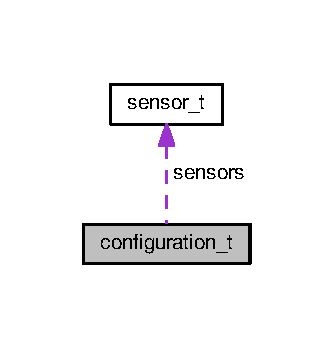
\includegraphics[width=160pt]{structconfiguration__t__coll__graph}
\end{center}
\end{figure}
\subsection*{Public Attributes}
\begin{DoxyCompactItemize}
\item 
\mbox{\Hypertarget{structconfiguration__t_a32d4c4bb78b5b231704c8a9f8d1b9e87}\label{structconfiguration__t_a32d4c4bb78b5b231704c8a9f8d1b9e87}} 
uint8\+\_\+t \hyperlink{structconfiguration__t_a32d4c4bb78b5b231704c8a9f8d1b9e87}{module\+\_\+version}
\begin{DoxyCompactList}\small\item\em module version \end{DoxyCompactList}\item 
\mbox{\Hypertarget{structconfiguration__t_a7dab895a0a9aa44bb65d90ef8016127d}\label{structconfiguration__t_a7dab895a0a9aa44bb65d90ef8016127d}} 
uint8\+\_\+t \hyperlink{structconfiguration__t_a7dab895a0a9aa44bb65d90ef8016127d}{module\+\_\+type}
\begin{DoxyCompactList}\small\item\em module type \end{DoxyCompactList}\item 
\mbox{\Hypertarget{structconfiguration__t_a0e088540266e347426ae73aed159f63a}\label{structconfiguration__t_a0e088540266e347426ae73aed159f63a}} 
uint8\+\_\+t \hyperlink{structconfiguration__t_a0e088540266e347426ae73aed159f63a}{i2c\+\_\+address}
\begin{DoxyCompactList}\small\item\em i2c address \end{DoxyCompactList}\item 
\mbox{\Hypertarget{structconfiguration__t_a227ef462f171f25e31cb3b0ce70b2597}\label{structconfiguration__t_a227ef462f171f25e31cb3b0ce70b2597}} 
bool \hyperlink{structconfiguration__t_a227ef462f171f25e31cb3b0ce70b2597}{is\+\_\+oneshot}
\begin{DoxyCompactList}\small\item\em enable or disable oneshot mode \end{DoxyCompactList}\item 
\mbox{\Hypertarget{structconfiguration__t_a33f99299576a58b3eb55be371e143531}\label{structconfiguration__t_a33f99299576a58b3eb55be371e143531}} 
bool \hyperlink{structconfiguration__t_a33f99299576a58b3eb55be371e143531}{is\+\_\+continuous}
\begin{DoxyCompactList}\small\item\em enable or disable continuous mode \end{DoxyCompactList}\item 
\mbox{\Hypertarget{structconfiguration__t_aed0a51c0dfbd925368c8539cf10c3001}\label{structconfiguration__t_aed0a51c0dfbd925368c8539cf10c3001}} 
uint8\+\_\+t \hyperlink{structconfiguration__t_aed0a51c0dfbd925368c8539cf10c3001}{i2c\+\_\+temperature\+\_\+address}
\begin{DoxyCompactList}\small\item\em i2c address of temperature sensor \end{DoxyCompactList}\item 
\mbox{\Hypertarget{structconfiguration__t_a79d1b1d9cb095c2bc0deb36c4f44452c}\label{structconfiguration__t_a79d1b1d9cb095c2bc0deb36c4f44452c}} 
uint8\+\_\+t \hyperlink{structconfiguration__t_a79d1b1d9cb095c2bc0deb36c4f44452c}{i2c\+\_\+humidity\+\_\+address}
\begin{DoxyCompactList}\small\item\em i2c address of humidity sensor \end{DoxyCompactList}\item 
\mbox{\Hypertarget{structconfiguration__t_adede74f3da6d26f5bc4b5e64e4776f7f}\label{structconfiguration__t_adede74f3da6d26f5bc4b5e64e4776f7f}} 
\hyperlink{structsensor__t}{sensor\+\_\+t} \hyperlink{structconfiguration__t_adede74f3da6d26f5bc4b5e64e4776f7f}{sensors} \mbox{[}\hyperlink{rmap-config_8h_af18dc3de744722cb308451b7a705611b}{U\+S\+E\+\_\+\+S\+E\+N\+S\+O\+R\+S\+\_\+\+C\+O\+U\+NT}\mbox{]}
\begin{DoxyCompactList}\small\item\em \hyperlink{classSensorDriver}{Sensor\+Driver} buffer for storing sensors parameter. \end{DoxyCompactList}\item 
\mbox{\Hypertarget{structconfiguration__t_a9a1e7c702c2dd7270f31aca29264db86}\label{structconfiguration__t_a9a1e7c702c2dd7270f31aca29264db86}} 
uint8\+\_\+t \hyperlink{structconfiguration__t_a9a1e7c702c2dd7270f31aca29264db86}{sensors\+\_\+count}
\begin{DoxyCompactList}\small\item\em configured sensors number \end{DoxyCompactList}\item 
\mbox{\Hypertarget{structconfiguration__t_a0c0dc512cf86464d2e8dad486e042c5c}\label{structconfiguration__t_a0c0dc512cf86464d2e8dad486e042c5c}} 
uint16\+\_\+t \hyperlink{structconfiguration__t_a0c0dc512cf86464d2e8dad486e042c5c}{report\+\_\+seconds}
\begin{DoxyCompactList}\small\item\em seconds for report values \end{DoxyCompactList}\item 
\mbox{\Hypertarget{structconfiguration__t_a04554256dd43582433092cd70dd8b87d}\label{structconfiguration__t_a04554256dd43582433092cd70dd8b87d}} 
bool \hyperlink{structconfiguration__t_a04554256dd43582433092cd70dd8b87d}{is\+\_\+dhcp\+\_\+enable}
\begin{DoxyCompactList}\small\item\em dhcp status \end{DoxyCompactList}\item 
\mbox{\Hypertarget{structconfiguration__t_a6ade77826c87e62532cae8ca0f045dac}\label{structconfiguration__t_a6ade77826c87e62532cae8ca0f045dac}} 
uint8\+\_\+t \hyperlink{structconfiguration__t_a6ade77826c87e62532cae8ca0f045dac}{ethernet\+\_\+mac} \mbox{[}\hyperlink{ethernet__config_8h_aafad911924144dbfc03b66b146ed4439}{E\+T\+H\+E\+R\+N\+E\+T\+\_\+\+M\+A\+C\+\_\+\+L\+E\+N\+G\+TH}\mbox{]}
\begin{DoxyCompactList}\small\item\em ethernet mac \end{DoxyCompactList}\item 
\mbox{\Hypertarget{structconfiguration__t_a0b698acfbb52f889c906b9b175f7a5d5}\label{structconfiguration__t_a0b698acfbb52f889c906b9b175f7a5d5}} 
uint8\+\_\+t \hyperlink{structconfiguration__t_a0b698acfbb52f889c906b9b175f7a5d5}{ip} \mbox{[}\hyperlink{ethernet__config_8h_ae8de53528e88d8ff4516d82a48590bd7}{E\+T\+H\+E\+R\+N\+E\+T\+\_\+\+I\+P\+\_\+\+L\+E\+N\+G\+TH}\mbox{]}
\begin{DoxyCompactList}\small\item\em ip address \end{DoxyCompactList}\item 
\mbox{\Hypertarget{structconfiguration__t_a60716ed8c6a82119a46eb6345b88ca32}\label{structconfiguration__t_a60716ed8c6a82119a46eb6345b88ca32}} 
uint8\+\_\+t \hyperlink{structconfiguration__t_a60716ed8c6a82119a46eb6345b88ca32}{netmask} \mbox{[}\hyperlink{ethernet__config_8h_ae8de53528e88d8ff4516d82a48590bd7}{E\+T\+H\+E\+R\+N\+E\+T\+\_\+\+I\+P\+\_\+\+L\+E\+N\+G\+TH}\mbox{]}
\begin{DoxyCompactList}\small\item\em netmask \end{DoxyCompactList}\item 
\mbox{\Hypertarget{structconfiguration__t_a9d18b7f4094f4d7a50d2245e0370adc0}\label{structconfiguration__t_a9d18b7f4094f4d7a50d2245e0370adc0}} 
uint8\+\_\+t \hyperlink{structconfiguration__t_a9d18b7f4094f4d7a50d2245e0370adc0}{gateway} \mbox{[}\hyperlink{ethernet__config_8h_ae8de53528e88d8ff4516d82a48590bd7}{E\+T\+H\+E\+R\+N\+E\+T\+\_\+\+I\+P\+\_\+\+L\+E\+N\+G\+TH}\mbox{]}
\begin{DoxyCompactList}\small\item\em gateway \end{DoxyCompactList}\item 
\mbox{\Hypertarget{structconfiguration__t_acd481c434576a90959c342e877985b32}\label{structconfiguration__t_acd481c434576a90959c342e877985b32}} 
uint8\+\_\+t \hyperlink{structconfiguration__t_acd481c434576a90959c342e877985b32}{primary\+\_\+dns} \mbox{[}\hyperlink{ethernet__config_8h_ae8de53528e88d8ff4516d82a48590bd7}{E\+T\+H\+E\+R\+N\+E\+T\+\_\+\+I\+P\+\_\+\+L\+E\+N\+G\+TH}\mbox{]}
\begin{DoxyCompactList}\small\item\em primary dns \end{DoxyCompactList}\end{DoxyCompactItemize}


\subsection{Detailed Description}
E\+E\+P\+R\+OM saved configuration. 

The documentation for this struct was generated from the following files\+:\begin{DoxyCompactItemize}
\item 
sketchbook/rmap/i2c-\/rain/\hyperlink{i2c-rain_8h}{i2c-\/rain.\+h}\item 
sketchbook/rmap/i2c-\/th/\hyperlink{i2c-th_8h}{i2c-\/th.\+h}\item 
sketchbook/rmap/rmap/\hyperlink{rmap_8h}{rmap.\+h}\end{DoxyCompactItemize}

\hypertarget{structFuncMap}{}\section{Func\+Map Struct Reference}
\label{structFuncMap}\index{Func\+Map@{Func\+Map}}


Collaboration diagram for Func\+Map\+:\nopagebreak
\begin{figure}[H]
\begin{center}
\leavevmode
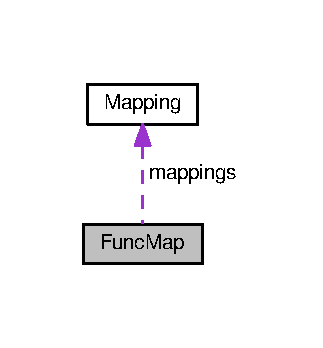
\includegraphics[width=155pt]{structFuncMap__coll__graph}
\end{center}
\end{figure}
\subsection*{Public Attributes}
\begin{DoxyCompactItemize}
\item 
\mbox{\Hypertarget{structFuncMap_ad53d8c1e8ff7a75eefe1fa0dd4ccd9bc}\label{structFuncMap_ad53d8c1e8ff7a75eefe1fa0dd4ccd9bc}} 
\hyperlink{structMapping}{Mapping} {\bfseries mappings} \mbox{[}J\+R\+P\+C\+\_\+\+M\+A\+X\+R\+PC\mbox{]}
\item 
\mbox{\Hypertarget{structFuncMap_ac342e66255d678322bd31f5d1e4f29b9}\label{structFuncMap_ac342e66255d678322bd31f5d1e4f29b9}} 
unsigned int {\bfseries used}
\end{DoxyCompactItemize}


The documentation for this struct was generated from the following files\+:\begin{DoxyCompactItemize}
\item 
sketchbook/libraries/arduino\+Json\+R\+P\+C/arduino\+Json\+R\+P\+C.\+h\item 
sketchbook/libraries/arduino\+Json\+R\+P\+C/arduino\+Json\+R\+P\+C.\+cpp\end{DoxyCompactItemize}

\hypertarget{classJsonRPC}{}\section{Json\+R\+PC Class Reference}
\label{classJsonRPC}\index{Json\+R\+PC@{Json\+R\+PC}}
\subsection*{Public Member Functions}
\begin{DoxyCompactItemize}
\item 
\mbox{\Hypertarget{classJsonRPC_a617c430786b5dbce52a312ef80c3957b}\label{classJsonRPC_a617c430786b5dbce52a312ef80c3957b}} 
{\bfseries Json\+R\+PC} (bool my\+\_\+radio=false)
\item 
\mbox{\Hypertarget{classJsonRPC_aae0b81ab3de6cf64c72e0330291555b9}\label{classJsonRPC_aae0b81ab3de6cf64c72e0330291555b9}} 
int {\bfseries parse\+Stream} (bool $\ast$is\+\_\+active, Stream $\ast$stream, uint32\+\_\+t timeout=J\+R\+P\+C\+\_\+\+D\+E\+F\+A\+U\+L\+T\+\_\+\+T\+I\+M\+E\+O\+U\+T\+\_\+\+MS)
\item 
\mbox{\Hypertarget{classJsonRPC_a011e5dec59c8ef72a3ffe08442afa98c}\label{classJsonRPC_a011e5dec59c8ef72a3ffe08442afa98c}} 
int {\bfseries callback} (Stream $\ast$stream)
\item 
\mbox{\Hypertarget{classJsonRPC_a2d24ec53b8142bb542a3ab89bf56dd22}\label{classJsonRPC_a2d24ec53b8142bb542a3ab89bf56dd22}} 
void {\bfseries register\+Method} (const char $\ast$method\+Name, int($\ast$callback)(Json\+Object \&, Json\+Object \&))
\item 
\mbox{\Hypertarget{classJsonRPC_a6ce8b0716779077a3decf3a0e928308c}\label{classJsonRPC_a6ce8b0716779077a3decf3a0e928308c}} 
int {\bfseries process\+Message} (Json\+Object \&msg)
\end{DoxyCompactItemize}
\subsection*{Public Attributes}
\begin{DoxyCompactItemize}
\item 
\mbox{\Hypertarget{classJsonRPC_a7dee13a51ff802762e2130d19c5ed3b9}\label{classJsonRPC_a7dee13a51ff802762e2130d19c5ed3b9}} 
char {\bfseries input\+\_\+buffer} \mbox{[}J\+R\+P\+C\+\_\+\+B\+U\+F\+F\+E\+R\+\_\+\+L\+E\+N\+G\+TH\mbox{]}
\end{DoxyCompactItemize}


The documentation for this class was generated from the following files\+:\begin{DoxyCompactItemize}
\item 
sketchbook/libraries/arduino\+Json\+R\+P\+C/arduino\+Json\+R\+P\+C.\+h\item 
sketchbook/libraries/arduino\+Json\+R\+P\+C/arduino\+Json\+R\+P\+C.\+cpp\end{DoxyCompactItemize}

\hypertarget{structMapping}{}\section{Mapping Struct Reference}
\label{structMapping}\index{Mapping@{Mapping}}
\subsection*{Public Attributes}
\begin{DoxyCompactItemize}
\item 
\mbox{\Hypertarget{structMapping_a6fed520d4d18b07e6f435751f70fa31d}\label{structMapping_a6fed520d4d18b07e6f435751f70fa31d}} 
char {\bfseries name} \mbox{[}J\+R\+P\+C\+\_\+\+M\+A\+X\+R\+P\+C\+N\+A\+M\+E\+L\+EN\mbox{]}
\item 
\mbox{\Hypertarget{structMapping_ac186e72e69faab3f56dc1e414986da72}\label{structMapping_ac186e72e69faab3f56dc1e414986da72}} 
int($\ast$ {\bfseries callback} )(Json\+Object \&, Json\+Object \&)
\end{DoxyCompactItemize}


The documentation for this struct was generated from the following files\+:\begin{DoxyCompactItemize}
\item 
sketchbook/libraries/arduino\+Json\+R\+P\+C/arduino\+Json\+R\+P\+C.\+h\item 
sketchbook/libraries/arduino\+Json\+R\+P\+C/arduino\+Json\+R\+P\+C.\+cpp\end{DoxyCompactItemize}

\input{classNtp}
\input{structobservation__t}
\input{structrain__t}
\hypertarget{structreadable__data__t}{}\section{readable\+\_\+data\+\_\+t Struct Reference}
\label{structreadable__data__t}\index{readable\+\_\+data\+\_\+t@{readable\+\_\+data\+\_\+t}}


Readable data through i2c bus.  




{\ttfamily \#include $<$i2c-\/rain.\+h$>$}



Collaboration diagram for readable\+\_\+data\+\_\+t\+:\nopagebreak
\begin{figure}[H]
\begin{center}
\leavevmode
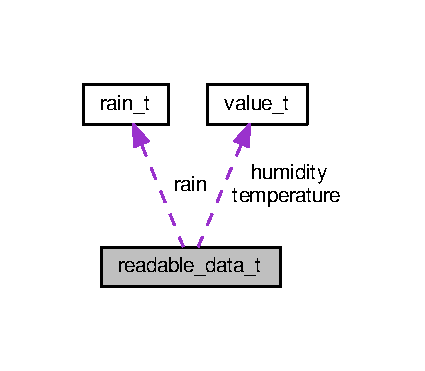
\includegraphics[width=204pt]{structreadable__data__t__coll__graph}
\end{center}
\end{figure}
\subsection*{Public Attributes}
\begin{DoxyCompactItemize}
\item 
\mbox{\Hypertarget{structreadable__data__t_a650c71ad521e965abe34eafda7cf872d}\label{structreadable__data__t_a650c71ad521e965abe34eafda7cf872d}} 
uint8\+\_\+t \hyperlink{structreadable__data__t_a650c71ad521e965abe34eafda7cf872d}{module\+\_\+type}
\begin{DoxyCompactList}\small\item\em module version \end{DoxyCompactList}\item 
\mbox{\Hypertarget{structreadable__data__t_a0b5fa5d2d89bef1b53036512525127f0}\label{structreadable__data__t_a0b5fa5d2d89bef1b53036512525127f0}} 
uint8\+\_\+t \hyperlink{structreadable__data__t_a0b5fa5d2d89bef1b53036512525127f0}{module\+\_\+version}
\begin{DoxyCompactList}\small\item\em module type \end{DoxyCompactList}\item 
\mbox{\Hypertarget{structreadable__data__t_a183ab6eb973fe8deb1c6d0583a991e92}\label{structreadable__data__t_a183ab6eb973fe8deb1c6d0583a991e92}} 
\hyperlink{structrain__t}{rain\+\_\+t} \hyperlink{structreadable__data__t_a183ab6eb973fe8deb1c6d0583a991e92}{rain}
\begin{DoxyCompactList}\small\item\em rain data \end{DoxyCompactList}\item 
\mbox{\Hypertarget{structreadable__data__t_a5852a1cd826e865b18a07fa4be784c6d}\label{structreadable__data__t_a5852a1cd826e865b18a07fa4be784c6d}} 
\hyperlink{structvalue__t}{value\+\_\+t} \hyperlink{structreadable__data__t_a5852a1cd826e865b18a07fa4be784c6d}{temperature}
\begin{DoxyCompactList}\small\item\em temperature data for report \end{DoxyCompactList}\item 
\mbox{\Hypertarget{structreadable__data__t_ab296c803ef271e46364679c955711e26}\label{structreadable__data__t_ab296c803ef271e46364679c955711e26}} 
\hyperlink{structvalue__t}{value\+\_\+t} \hyperlink{structreadable__data__t_ab296c803ef271e46364679c955711e26}{humidity}
\begin{DoxyCompactList}\small\item\em humidity data for report \end{DoxyCompactList}\end{DoxyCompactItemize}


\subsection{Detailed Description}
Readable data through i2c bus. 

The documentation for this struct was generated from the following files\+:\begin{DoxyCompactItemize}
\item 
sketchbook/rmap/i2c-\/rain/\hyperlink{i2c-rain_8h}{i2c-\/rain.\+h}\item 
sketchbook/rmap/i2c-\/th/\hyperlink{i2c-th_8h}{i2c-\/th.\+h}\end{DoxyCompactItemize}

\hypertarget{structsample__t}{}\section{sample\+\_\+t Struct Reference}
\label{structsample__t}\index{sample\+\_\+t@{sample\+\_\+t}}


Samples values for measured temperature and humidity.  




{\ttfamily \#include $<$i2c-\/th.\+h$>$}

\subsection*{Public Attributes}
\begin{DoxyCompactItemize}
\item 
\mbox{\Hypertarget{structsample__t_ab732cec6be98318b8f13563577f7d528}\label{structsample__t_ab732cec6be98318b8f13563577f7d528}} 
uint16\+\_\+t \hyperlink{structsample__t_ab732cec6be98318b8f13563577f7d528}{values} \mbox{[}\hyperlink{i2c-th-config_8h_a5500c7c28f9fc2cab4deffbe07c98b39}{S\+E\+N\+S\+O\+R\+S\+\_\+\+S\+A\+M\+P\+L\+E\+\_\+\+C\+O\+U\+N\+T\+\_\+\+M\+AX}\mbox{]}
\begin{DoxyCompactList}\small\item\em buffer containing the measured samples \end{DoxyCompactList}\item 
\mbox{\Hypertarget{structsample__t_a5a28abacf173c495a32a6f727e5d016e}\label{structsample__t_a5a28abacf173c495a32a6f727e5d016e}} 
uint8\+\_\+t \hyperlink{structsample__t_a5a28abacf173c495a32a6f727e5d016e}{count}
\begin{DoxyCompactList}\small\item\em number of samples \end{DoxyCompactList}\end{DoxyCompactItemize}


\subsection{Detailed Description}
Samples values for measured temperature and humidity. 

The documentation for this struct was generated from the following file\+:\begin{DoxyCompactItemize}
\item 
sketchbook/rmap/i2c-\/th/\hyperlink{i2c-th_8h}{i2c-\/th.\+h}\end{DoxyCompactItemize}

\hypertarget{structsensor__t}{}\section{sensor\+\_\+t Struct Reference}
\label{structsensor__t}\index{sensor\+\_\+t@{sensor\+\_\+t}}


Sensor struct for storing sensor configuration parameter.  




{\ttfamily \#include $<$typedef.\+h$>$}

\subsection*{Public Attributes}
\begin{DoxyCompactItemize}
\item 
\mbox{\Hypertarget{structsensor__t_aa5ebe8eef40ef912b7da2cb7391d2cf9}\label{structsensor__t_aa5ebe8eef40ef912b7da2cb7391d2cf9}} 
char \hyperlink{structsensor__t_aa5ebe8eef40ef912b7da2cb7391d2cf9}{driver} \mbox{[}\hyperlink{typedef_8h_a343127490097a8ef68ab7d577d01b38b}{D\+R\+I\+V\+E\+R\+\_\+\+L\+E\+N\+G\+TH}\mbox{]}
\begin{DoxyCompactList}\small\item\em sensor\textquotesingle{}s string driver \end{DoxyCompactList}\item 
\mbox{\Hypertarget{structsensor__t_a1a2280bc32299e544c7d740299102277}\label{structsensor__t_a1a2280bc32299e544c7d740299102277}} 
char \hyperlink{structsensor__t_a1a2280bc32299e544c7d740299102277}{type} \mbox{[}\hyperlink{typedef_8h_a7be6924e0d85f3f82149ea31cca36887}{T\+Y\+P\+E\+\_\+\+L\+E\+N\+G\+TH}\mbox{]}
\begin{DoxyCompactList}\small\item\em sensor\textquotesingle{}s string type \end{DoxyCompactList}\item 
\mbox{\Hypertarget{structsensor__t_aa8e66f9050a38bb842b5a97cc3bc2358}\label{structsensor__t_aa8e66f9050a38bb842b5a97cc3bc2358}} 
uint8\+\_\+t \hyperlink{structsensor__t_aa8e66f9050a38bb842b5a97cc3bc2358}{address}
\begin{DoxyCompactList}\small\item\em sensor\textquotesingle{}s address \end{DoxyCompactList}\item 
\mbox{\Hypertarget{structsensor__t_a907c65079d3374ff1f18532cf41ccf13}\label{structsensor__t_a907c65079d3374ff1f18532cf41ccf13}} 
uint8\+\_\+t \hyperlink{structsensor__t_a907c65079d3374ff1f18532cf41ccf13}{node}
\begin{DoxyCompactList}\small\item\em sensor\textquotesingle{}s node \end{DoxyCompactList}\item 
\mbox{\Hypertarget{structsensor__t_a08e3c60cbf75700af6e9529621bfd51f}\label{structsensor__t_a08e3c60cbf75700af6e9529621bfd51f}} 
char \hyperlink{structsensor__t_a08e3c60cbf75700af6e9529621bfd51f}{mqtt\+\_\+topic} \mbox{[}\hyperlink{mqtt__config_8h_a85772fcdfe85fa51f02f3045c0aa7764}{M\+Q\+T\+T\+\_\+\+S\+E\+N\+S\+O\+R\+\_\+\+T\+O\+P\+I\+C\+\_\+\+L\+E\+N\+G\+TH}\mbox{]}
\begin{DoxyCompactList}\small\item\em sensor\textquotesingle{}s mqtt topic path \end{DoxyCompactList}\end{DoxyCompactItemize}


\subsection{Detailed Description}
Sensor struct for storing sensor configuration parameter. 

The documentation for this struct was generated from the following file\+:\begin{DoxyCompactItemize}
\item 
sketchbook/libraries/\+Rmap/\hyperlink{typedef_8h}{typedef.\+h}\end{DoxyCompactItemize}

\hypertarget{classSensorDriver}{}\section{Sensor\+Driver Class Reference}
\label{classSensorDriver}\index{Sensor\+Driver@{Sensor\+Driver}}


\hyperlink{classSensorDriver}{Sensor\+Driver} class.  




{\ttfamily \#include $<$Sensor\+Driver.\+h$>$}

\subsection*{Public Member Functions}
\begin{DoxyCompactItemize}
\item 
\hyperlink{classSensorDriver_ab09b984c0201774e2e1eba23d2fb775d}{Sensor\+Driver} (const char $\ast$driver, const char $\ast$type)
\begin{DoxyCompactList}\small\item\em Constructor for \hyperlink{classSensorDriver}{Sensor\+Driver}. \end{DoxyCompactList}\item 
virtual void \hyperlink{classSensorDriver_ad6d2e1e9bf26944f102af3042ba1c615}{setup} (const uint8\+\_\+t address, const uint8\+\_\+t node=0)
\begin{DoxyCompactList}\small\item\em Setup sensor. \end{DoxyCompactList}\item 
virtual void \hyperlink{classSensorDriver_a19e0acad6518cf382fe7e71a7b915506}{prepare} ()
\begin{DoxyCompactList}\small\item\em Prepare sensor. \end{DoxyCompactList}\item 
virtual void \hyperlink{classSensorDriver_a2d9da1147c103028eff6756c3467f486}{get} (int32\+\_\+t $\ast$\hyperlink{classSensorDriver_a133e97d4b06f8b4d12265df0ac0bf9ed}{values}, uint8\+\_\+t length)
\begin{DoxyCompactList}\small\item\em Get value from sensor. \end{DoxyCompactList}\item 
const char $\ast$ \hyperlink{classSensorDriver_a5056f9f058d069b9840a6045c1a652d3}{get\+Driver} ()
\begin{DoxyCompactList}\small\item\em Get the sensor\textquotesingle{}s driver. \end{DoxyCompactList}\item 
const char $\ast$ \hyperlink{classSensorDriver_a3d87944d9f86320f645af7dad549e4a8}{get\+Type} ()
\begin{DoxyCompactList}\small\item\em Get the sensor\textquotesingle{}s type. \end{DoxyCompactList}\item 
uint8\+\_\+t \hyperlink{classSensorDriver_a3f0ac74e7502159bac092a1fd4d05dda}{get\+Address} ()
\begin{DoxyCompactList}\small\item\em Get the sensor\textquotesingle{}s address. \end{DoxyCompactList}\item 
uint8\+\_\+t \hyperlink{classSensorDriver_a30e20150ec52e3ec3a7257978e533618}{get\+Node} ()
\begin{DoxyCompactList}\small\item\em Get the sensor\textquotesingle{}s node. \end{DoxyCompactList}\item 
uint32\+\_\+t \hyperlink{classSensorDriver_a8636758f202044a24e916d10bf339f10}{get\+Start\+Time} ()
\begin{DoxyCompactList}\small\item\em Get the last setted sensor\textquotesingle{}s start time. \end{DoxyCompactList}\item 
uint32\+\_\+t \hyperlink{classSensorDriver_a432c4878ec9ca5145a4bdd827ebbc7d7}{get\+Delay} ()
\begin{DoxyCompactList}\small\item\em Get the last setted sensor\textquotesingle{}s delay. \end{DoxyCompactList}\item 
bool \hyperlink{classSensorDriver_a8ababf180e52d684416bc6f4c4f90e59}{is\+End} ()
\begin{DoxyCompactList}\small\item\em Check if get sequence is complete. \end{DoxyCompactList}\item 
bool \hyperlink{classSensorDriver_af8d094335bc75fbf1390ee5b498eec69}{is\+Success} ()
\begin{DoxyCompactList}\small\item\em Check if get sequence is complete with success. \end{DoxyCompactList}\item 
bool \hyperlink{classSensorDriver_a65f1930e35568439dee39259a23a5670}{is\+Readed} ()
\begin{DoxyCompactList}\small\item\em Check if values were readed from sensor. \end{DoxyCompactList}\item 
virtual bool \hyperlink{classSensorDriver_a0f64839cf7719b5782c93e54485d3b11}{is\+Setted} ()
\begin{DoxyCompactList}\small\item\em Check if sensor was setted. \end{DoxyCompactList}\item 
virtual bool \hyperlink{classSensorDriver_a17672e5f12749c3dca5d6c2c4b73b7c3}{is\+Prepared} ()
\begin{DoxyCompactList}\small\item\em Check if sensor was preapared. \end{DoxyCompactList}\item 
virtual void \hyperlink{classSensorDriver_a2b347ee438af49b939cb1e79c068681f}{reset\+Prepared} ()
\begin{DoxyCompactList}\small\item\em Reset preapred internal state of sensor. \end{DoxyCompactList}\end{DoxyCompactItemize}
\subsection*{Static Public Member Functions}
\begin{DoxyCompactItemize}
\item 
static \hyperlink{classSensorDriver}{Sensor\+Driver} $\ast$ \hyperlink{classSensorDriver_a42e3b501ef28a0a8ba7e045f84e3d76a}{create} (const char $\ast$driver, const char $\ast$type)
\begin{DoxyCompactList}\small\item\em Create an instance of \hyperlink{classSensorDriver}{Sensor\+Driver} for specific sensor. \end{DoxyCompactList}\item 
static void \hyperlink{classSensorDriver_a8b3cc902953a0850241c625772757580}{create\+And\+Setup} (const char $\ast$driver, const char $\ast$type, const uint8\+\_\+t address, const uint8\+\_\+t node, \hyperlink{classSensorDriver}{Sensor\+Driver} $\ast$\hyperlink{i2c-th_8h_a5f5c708cbddb6cef952fb9a28c8ba835}{sensors}\mbox{[}$\,$\mbox{]}, uint8\+\_\+t $\ast$\hyperlink{i2c-th_8h_a7727577f63dfa4aa55feb7ddd0739f83}{sensors\+\_\+count})
\begin{DoxyCompactList}\small\item\em Create and setup the specified sensor. \end{DoxyCompactList}\end{DoxyCompactItemize}
\subsection*{Static Protected Member Functions}
\begin{DoxyCompactItemize}
\item 
static void \hyperlink{classSensorDriver_acaeaeab0b4536073c812bf53582a9e08}{print\+Info} (const char $\ast$driver, const char $\ast$type, const uint8\+\_\+t address=0, const uint8\+\_\+t node=0)
\begin{DoxyCompactList}\small\item\em Print information about sensor. \end{DoxyCompactList}\end{DoxyCompactItemize}
\subsection*{Protected Attributes}
\begin{DoxyCompactItemize}
\item 
\mbox{\Hypertarget{classSensorDriver_af4563562f35c54710cdff4d41d596100}\label{classSensorDriver_af4563562f35c54710cdff4d41d596100}} 
const char $\ast$ \hyperlink{classSensorDriver_af4563562f35c54710cdff4d41d596100}{\+\_\+driver}
\begin{DoxyCompactList}\small\item\em Internal sensor\textquotesingle{}s variable for driver. \end{DoxyCompactList}\item 
\mbox{\Hypertarget{classSensorDriver_a545ce08f6016a2fa0e3aebcca51edcbd}\label{classSensorDriver_a545ce08f6016a2fa0e3aebcca51edcbd}} 
const char $\ast$ \hyperlink{classSensorDriver_a545ce08f6016a2fa0e3aebcca51edcbd}{\+\_\+type}
\begin{DoxyCompactList}\small\item\em Internal sensor\textquotesingle{}s variable for type. \end{DoxyCompactList}\item 
\mbox{\Hypertarget{classSensorDriver_a13853dc3219d536dd19553768f053688}\label{classSensorDriver_a13853dc3219d536dd19553768f053688}} 
uint8\+\_\+t \hyperlink{classSensorDriver_a13853dc3219d536dd19553768f053688}{\+\_\+address}
\begin{DoxyCompactList}\small\item\em Internal sensor\textquotesingle{}s variable for address. \end{DoxyCompactList}\item 
\mbox{\Hypertarget{classSensorDriver_a48e9eb12164eb73dc1ce6a14e042a4d3}\label{classSensorDriver_a48e9eb12164eb73dc1ce6a14e042a4d3}} 
uint8\+\_\+t \hyperlink{classSensorDriver_a48e9eb12164eb73dc1ce6a14e042a4d3}{\+\_\+node}
\begin{DoxyCompactList}\small\item\em Internal sensor\textquotesingle{}s variable for node. \end{DoxyCompactList}\item 
\mbox{\Hypertarget{classSensorDriver_a25a43cc518d9fbc09e84c709bf293c56}\label{classSensorDriver_a25a43cc518d9fbc09e84c709bf293c56}} 
uint32\+\_\+t \hyperlink{classSensorDriver_a25a43cc518d9fbc09e84c709bf293c56}{\+\_\+delay\+\_\+ms}
\begin{DoxyCompactList}\small\item\em Internal sensor\textquotesingle{}s variable for delay. \end{DoxyCompactList}\item 
\mbox{\Hypertarget{classSensorDriver_a542b221f1e79b72badf2b4c68883111b}\label{classSensorDriver_a542b221f1e79b72badf2b4c68883111b}} 
uint32\+\_\+t \hyperlink{classSensorDriver_a542b221f1e79b72badf2b4c68883111b}{\+\_\+start\+\_\+time\+\_\+ms}
\begin{DoxyCompactList}\small\item\em Internal sensor\textquotesingle{}s variable for start time milliseconds. \end{DoxyCompactList}\item 
\mbox{\Hypertarget{classSensorDriver_a133e97d4b06f8b4d12265df0ac0bf9ed}\label{classSensorDriver_a133e97d4b06f8b4d12265df0ac0bf9ed}} 
int32\+\_\+t \hyperlink{classSensorDriver_a133e97d4b06f8b4d12265df0ac0bf9ed}{values} \mbox{[}$\,$\mbox{]}
\begin{DoxyCompactList}\small\item\em Internal sensor\textquotesingle{}s variable for values readed from sensors. \end{DoxyCompactList}\item 
\mbox{\Hypertarget{classSensorDriver_ab3c5ceebf49b96af8a9f96d7cc6fdef8}\label{classSensorDriver_ab3c5ceebf49b96af8a9f96d7cc6fdef8}} 
bool \hyperlink{classSensorDriver_ab3c5ceebf49b96af8a9f96d7cc6fdef8}{\+\_\+is\+\_\+end}
\begin{DoxyCompactList}\small\item\em Internal sensor\textquotesingle{}s variable for save end of reading values. \end{DoxyCompactList}\item 
\mbox{\Hypertarget{classSensorDriver_a80a57f982b9d5eb776a34ecc601334b3}\label{classSensorDriver_a80a57f982b9d5eb776a34ecc601334b3}} 
bool \hyperlink{classSensorDriver_a80a57f982b9d5eb776a34ecc601334b3}{\+\_\+is\+\_\+success}
\begin{DoxyCompactList}\small\item\em Internal sensor\textquotesingle{}s variable for save if readed was successful. \end{DoxyCompactList}\item 
\mbox{\Hypertarget{classSensorDriver_a7a418701714073a0768c2b1ce1104c2b}\label{classSensorDriver_a7a418701714073a0768c2b1ce1104c2b}} 
bool \hyperlink{classSensorDriver_a7a418701714073a0768c2b1ce1104c2b}{\+\_\+is\+\_\+readed}
\begin{DoxyCompactList}\small\item\em Internal sensor\textquotesingle{}s variable for save is readed. \end{DoxyCompactList}\end{DoxyCompactItemize}


\subsection{Detailed Description}
\hyperlink{classSensorDriver}{Sensor\+Driver} class. 

\subsection{Constructor \& Destructor Documentation}
\mbox{\Hypertarget{classSensorDriver_ab09b984c0201774e2e1eba23d2fb775d}\label{classSensorDriver_ab09b984c0201774e2e1eba23d2fb775d}} 
\index{Sensor\+Driver@{Sensor\+Driver}!Sensor\+Driver@{Sensor\+Driver}}
\index{Sensor\+Driver@{Sensor\+Driver}!Sensor\+Driver@{Sensor\+Driver}}
\subsubsection{\texorpdfstring{Sensor\+Driver()}{SensorDriver()}}
{\footnotesize\ttfamily Sensor\+Driver\+::\+Sensor\+Driver (\begin{DoxyParamCaption}\item[{const char $\ast$}]{driver,  }\item[{const char $\ast$}]{type }\end{DoxyParamCaption})}



Constructor for \hyperlink{classSensorDriver}{Sensor\+Driver}. 


\begin{DoxyParams}[1]{Parameters}
\mbox{\tt in}  & {\em $\ast$driver} & driver\textquotesingle{}s type. \\
\hline
\mbox{\tt in}  & {\em $\ast$type} & sensor\textquotesingle{}s type. \\
\hline
\end{DoxyParams}
\begin{DoxyReturn}{Returns}
void. 
\end{DoxyReturn}


\subsection{Member Function Documentation}
\mbox{\Hypertarget{classSensorDriver_a42e3b501ef28a0a8ba7e045f84e3d76a}\label{classSensorDriver_a42e3b501ef28a0a8ba7e045f84e3d76a}} 
\index{Sensor\+Driver@{Sensor\+Driver}!create@{create}}
\index{create@{create}!Sensor\+Driver@{Sensor\+Driver}}
\subsubsection{\texorpdfstring{create()}{create()}}
{\footnotesize\ttfamily \hyperlink{classSensorDriver}{Sensor\+Driver} $\ast$ Sensor\+Driver\+::create (\begin{DoxyParamCaption}\item[{const char $\ast$}]{driver,  }\item[{const char $\ast$}]{type }\end{DoxyParamCaption})\hspace{0.3cm}{\ttfamily [static]}}



Create an instance of \hyperlink{classSensorDriver}{Sensor\+Driver} for specific sensor. 


\begin{DoxyParams}[1]{Parameters}
\mbox{\tt in}  & {\em $\ast$driver} & driver\textquotesingle{}s type. \\
\hline
\mbox{\tt in}  & {\em $\ast$type} & sensor\textquotesingle{}s type. \\
\hline
\end{DoxyParams}
\begin{DoxyReturn}{Returns}
instance of \hyperlink{classSensorDriver}{Sensor\+Driver} for specified sensor. 
\end{DoxyReturn}
\mbox{\Hypertarget{classSensorDriver_a8b3cc902953a0850241c625772757580}\label{classSensorDriver_a8b3cc902953a0850241c625772757580}} 
\index{Sensor\+Driver@{Sensor\+Driver}!create\+And\+Setup@{create\+And\+Setup}}
\index{create\+And\+Setup@{create\+And\+Setup}!Sensor\+Driver@{Sensor\+Driver}}
\subsubsection{\texorpdfstring{create\+And\+Setup()}{createAndSetup()}}
{\footnotesize\ttfamily void Sensor\+Driver\+::create\+And\+Setup (\begin{DoxyParamCaption}\item[{const char $\ast$}]{driver,  }\item[{const char $\ast$}]{type,  }\item[{const uint8\+\_\+t}]{address,  }\item[{const uint8\+\_\+t}]{node,  }\item[{\hyperlink{classSensorDriver}{Sensor\+Driver} $\ast$}]{sensors\mbox{[}$\,$\mbox{]},  }\item[{uint8\+\_\+t $\ast$}]{sensors\+\_\+count }\end{DoxyParamCaption})\hspace{0.3cm}{\ttfamily [static]}}



Create and setup the specified sensor. 


\begin{DoxyParams}[1]{Parameters}
\mbox{\tt in}  & {\em $\ast$driver} & driver\textquotesingle{}s type. \\
\hline
\mbox{\tt in}  & {\em $\ast$type} & sensor\textquotesingle{}s type. \\
\hline
\mbox{\tt in}  & {\em address} & sensor\textquotesingle{}s address. \\
\hline
\mbox{\tt in}  & {\em node} & sensor\textquotesingle{}s node. \\
\hline
\mbox{\tt in}  & {\em $\ast$sensors\mbox{[}$\,$\mbox{]}} & array of sensors. \\
\hline
\mbox{\tt in}  & {\em $\ast$sensors\+\_\+count} & setted sensors count. \\
\hline
\end{DoxyParams}
\begin{DoxyReturn}{Returns}
void. 
\end{DoxyReturn}
\mbox{\Hypertarget{classSensorDriver_a2d9da1147c103028eff6756c3467f486}\label{classSensorDriver_a2d9da1147c103028eff6756c3467f486}} 
\index{Sensor\+Driver@{Sensor\+Driver}!get@{get}}
\index{get@{get}!Sensor\+Driver@{Sensor\+Driver}}
\subsubsection{\texorpdfstring{get()}{get()}}
{\footnotesize\ttfamily void Sensor\+Driver\+::get (\begin{DoxyParamCaption}\item[{int32\+\_\+t $\ast$}]{values,  }\item[{uint8\+\_\+t}]{length }\end{DoxyParamCaption})\hspace{0.3cm}{\ttfamily [virtual]}}



Get value from sensor. 


\begin{DoxyParams}[1]{Parameters}
\mbox{\tt out}  & {\em $\ast$values} & pointer to array for getting multiple sensor\textquotesingle{}s value. \\
\hline
\mbox{\tt in}  & {\em length} & number of values readed from sensor. \\
\hline
\end{DoxyParams}
\begin{DoxyReturn}{Returns}
void. 
\end{DoxyReturn}
\mbox{\Hypertarget{classSensorDriver_a3f0ac74e7502159bac092a1fd4d05dda}\label{classSensorDriver_a3f0ac74e7502159bac092a1fd4d05dda}} 
\index{Sensor\+Driver@{Sensor\+Driver}!get\+Address@{get\+Address}}
\index{get\+Address@{get\+Address}!Sensor\+Driver@{Sensor\+Driver}}
\subsubsection{\texorpdfstring{get\+Address()}{getAddress()}}
{\footnotesize\ttfamily uint8\+\_\+t Sensor\+Driver\+::get\+Address (\begin{DoxyParamCaption}{ }\end{DoxyParamCaption})}



Get the sensor\textquotesingle{}s address. 

\begin{DoxyReturn}{Returns}
the sensor\textquotesingle{}s address. 
\end{DoxyReturn}
\mbox{\Hypertarget{classSensorDriver_a432c4878ec9ca5145a4bdd827ebbc7d7}\label{classSensorDriver_a432c4878ec9ca5145a4bdd827ebbc7d7}} 
\index{Sensor\+Driver@{Sensor\+Driver}!get\+Delay@{get\+Delay}}
\index{get\+Delay@{get\+Delay}!Sensor\+Driver@{Sensor\+Driver}}
\subsubsection{\texorpdfstring{get\+Delay()}{getDelay()}}
{\footnotesize\ttfamily uint32\+\_\+t Sensor\+Driver\+::get\+Delay (\begin{DoxyParamCaption}{ }\end{DoxyParamCaption})}



Get the last setted sensor\textquotesingle{}s delay. 

\begin{DoxyReturn}{Returns}
the sensor\textquotesingle{}s delay. 
\end{DoxyReturn}
\mbox{\Hypertarget{classSensorDriver_a5056f9f058d069b9840a6045c1a652d3}\label{classSensorDriver_a5056f9f058d069b9840a6045c1a652d3}} 
\index{Sensor\+Driver@{Sensor\+Driver}!get\+Driver@{get\+Driver}}
\index{get\+Driver@{get\+Driver}!Sensor\+Driver@{Sensor\+Driver}}
\subsubsection{\texorpdfstring{get\+Driver()}{getDriver()}}
{\footnotesize\ttfamily char $\ast$ Sensor\+Driver\+::get\+Driver (\begin{DoxyParamCaption}{ }\end{DoxyParamCaption})}



Get the sensor\textquotesingle{}s driver. 

\begin{DoxyReturn}{Returns}
the sensor\textquotesingle{}s driver. 
\end{DoxyReturn}
\mbox{\Hypertarget{classSensorDriver_a30e20150ec52e3ec3a7257978e533618}\label{classSensorDriver_a30e20150ec52e3ec3a7257978e533618}} 
\index{Sensor\+Driver@{Sensor\+Driver}!get\+Node@{get\+Node}}
\index{get\+Node@{get\+Node}!Sensor\+Driver@{Sensor\+Driver}}
\subsubsection{\texorpdfstring{get\+Node()}{getNode()}}
{\footnotesize\ttfamily uint8\+\_\+t Sensor\+Driver\+::get\+Node (\begin{DoxyParamCaption}{ }\end{DoxyParamCaption})}



Get the sensor\textquotesingle{}s node. 

\begin{DoxyReturn}{Returns}
the sensor\textquotesingle{}s node. 
\end{DoxyReturn}
\mbox{\Hypertarget{classSensorDriver_a8636758f202044a24e916d10bf339f10}\label{classSensorDriver_a8636758f202044a24e916d10bf339f10}} 
\index{Sensor\+Driver@{Sensor\+Driver}!get\+Start\+Time@{get\+Start\+Time}}
\index{get\+Start\+Time@{get\+Start\+Time}!Sensor\+Driver@{Sensor\+Driver}}
\subsubsection{\texorpdfstring{get\+Start\+Time()}{getStartTime()}}
{\footnotesize\ttfamily uint32\+\_\+t Sensor\+Driver\+::get\+Start\+Time (\begin{DoxyParamCaption}{ }\end{DoxyParamCaption})}



Get the last setted sensor\textquotesingle{}s start time. 

\begin{DoxyReturn}{Returns}
the sensor\textquotesingle{}s start time. 
\end{DoxyReturn}
\mbox{\Hypertarget{classSensorDriver_a3d87944d9f86320f645af7dad549e4a8}\label{classSensorDriver_a3d87944d9f86320f645af7dad549e4a8}} 
\index{Sensor\+Driver@{Sensor\+Driver}!get\+Type@{get\+Type}}
\index{get\+Type@{get\+Type}!Sensor\+Driver@{Sensor\+Driver}}
\subsubsection{\texorpdfstring{get\+Type()}{getType()}}
{\footnotesize\ttfamily char $\ast$ Sensor\+Driver\+::get\+Type (\begin{DoxyParamCaption}{ }\end{DoxyParamCaption})}



Get the sensor\textquotesingle{}s type. 

\begin{DoxyReturn}{Returns}
the sensor\textquotesingle{}s type. 
\end{DoxyReturn}
\mbox{\Hypertarget{classSensorDriver_a8ababf180e52d684416bc6f4c4f90e59}\label{classSensorDriver_a8ababf180e52d684416bc6f4c4f90e59}} 
\index{Sensor\+Driver@{Sensor\+Driver}!is\+End@{is\+End}}
\index{is\+End@{is\+End}!Sensor\+Driver@{Sensor\+Driver}}
\subsubsection{\texorpdfstring{is\+End()}{isEnd()}}
{\footnotesize\ttfamily bool Sensor\+Driver\+::is\+End (\begin{DoxyParamCaption}{ }\end{DoxyParamCaption})}



Check if get sequence is complete. 

\begin{DoxyReturn}{Returns}
true if complete, false otherwise. 
\end{DoxyReturn}
\mbox{\Hypertarget{classSensorDriver_a17672e5f12749c3dca5d6c2c4b73b7c3}\label{classSensorDriver_a17672e5f12749c3dca5d6c2c4b73b7c3}} 
\index{Sensor\+Driver@{Sensor\+Driver}!is\+Prepared@{is\+Prepared}}
\index{is\+Prepared@{is\+Prepared}!Sensor\+Driver@{Sensor\+Driver}}
\subsubsection{\texorpdfstring{is\+Prepared()}{isPrepared()}}
{\footnotesize\ttfamily bool Sensor\+Driver\+::is\+Prepared (\begin{DoxyParamCaption}{ }\end{DoxyParamCaption})\hspace{0.3cm}{\ttfamily [virtual]}}



Check if sensor was preapared. 

\begin{DoxyReturn}{Returns}
true if preapared, false otherwise. 
\end{DoxyReturn}
\mbox{\Hypertarget{classSensorDriver_a65f1930e35568439dee39259a23a5670}\label{classSensorDriver_a65f1930e35568439dee39259a23a5670}} 
\index{Sensor\+Driver@{Sensor\+Driver}!is\+Readed@{is\+Readed}}
\index{is\+Readed@{is\+Readed}!Sensor\+Driver@{Sensor\+Driver}}
\subsubsection{\texorpdfstring{is\+Readed()}{isReaded()}}
{\footnotesize\ttfamily bool Sensor\+Driver\+::is\+Readed (\begin{DoxyParamCaption}{ }\end{DoxyParamCaption})}



Check if values were readed from sensor. 

\begin{DoxyReturn}{Returns}
true if readed, false otherwise. 
\end{DoxyReturn}
\mbox{\Hypertarget{classSensorDriver_a0f64839cf7719b5782c93e54485d3b11}\label{classSensorDriver_a0f64839cf7719b5782c93e54485d3b11}} 
\index{Sensor\+Driver@{Sensor\+Driver}!is\+Setted@{is\+Setted}}
\index{is\+Setted@{is\+Setted}!Sensor\+Driver@{Sensor\+Driver}}
\subsubsection{\texorpdfstring{is\+Setted()}{isSetted()}}
{\footnotesize\ttfamily bool Sensor\+Driver\+::is\+Setted (\begin{DoxyParamCaption}{ }\end{DoxyParamCaption})\hspace{0.3cm}{\ttfamily [virtual]}}



Check if sensor was setted. 

\begin{DoxyReturn}{Returns}
true if setted, false otherwise. 
\end{DoxyReturn}
\mbox{\Hypertarget{classSensorDriver_af8d094335bc75fbf1390ee5b498eec69}\label{classSensorDriver_af8d094335bc75fbf1390ee5b498eec69}} 
\index{Sensor\+Driver@{Sensor\+Driver}!is\+Success@{is\+Success}}
\index{is\+Success@{is\+Success}!Sensor\+Driver@{Sensor\+Driver}}
\subsubsection{\texorpdfstring{is\+Success()}{isSuccess()}}
{\footnotesize\ttfamily bool Sensor\+Driver\+::is\+Success (\begin{DoxyParamCaption}{ }\end{DoxyParamCaption})}



Check if get sequence is complete with success. 

\begin{DoxyReturn}{Returns}
true if success, false otherwise. 
\end{DoxyReturn}
\mbox{\Hypertarget{classSensorDriver_a19e0acad6518cf382fe7e71a7b915506}\label{classSensorDriver_a19e0acad6518cf382fe7e71a7b915506}} 
\index{Sensor\+Driver@{Sensor\+Driver}!prepare@{prepare}}
\index{prepare@{prepare}!Sensor\+Driver@{Sensor\+Driver}}
\subsubsection{\texorpdfstring{prepare()}{prepare()}}
{\footnotesize\ttfamily void Sensor\+Driver\+::prepare (\begin{DoxyParamCaption}{ }\end{DoxyParamCaption})\hspace{0.3cm}{\ttfamily [virtual]}}



Prepare sensor. 

\begin{DoxyReturn}{Returns}
void. 
\end{DoxyReturn}
\mbox{\Hypertarget{classSensorDriver_acaeaeab0b4536073c812bf53582a9e08}\label{classSensorDriver_acaeaeab0b4536073c812bf53582a9e08}} 
\index{Sensor\+Driver@{Sensor\+Driver}!print\+Info@{print\+Info}}
\index{print\+Info@{print\+Info}!Sensor\+Driver@{Sensor\+Driver}}
\subsubsection{\texorpdfstring{print\+Info()}{printInfo()}}
{\footnotesize\ttfamily void Sensor\+Driver\+::print\+Info (\begin{DoxyParamCaption}\item[{const char $\ast$}]{driver,  }\item[{const char $\ast$}]{type,  }\item[{const uint8\+\_\+t}]{address = {\ttfamily 0},  }\item[{const uint8\+\_\+t}]{node = {\ttfamily 0} }\end{DoxyParamCaption})\hspace{0.3cm}{\ttfamily [static]}, {\ttfamily [protected]}}



Print information about sensor. 


\begin{DoxyParams}[1]{Parameters}
\mbox{\tt in}  & {\em $\ast$driver} & the sensor\textquotesingle{}s driver. \\
\hline
\mbox{\tt in}  & {\em $\ast$type} & the sensor\textquotesingle{}s type. \\
\hline
\mbox{\tt in}  & {\em address} & the sensor\textquotesingle{}s address. \\
\hline
\mbox{\tt in}  & {\em node} & the sensor\textquotesingle{}s node. \\
\hline
\end{DoxyParams}
\begin{DoxyReturn}{Returns}
void. 
\end{DoxyReturn}
\mbox{\Hypertarget{classSensorDriver_a2b347ee438af49b939cb1e79c068681f}\label{classSensorDriver_a2b347ee438af49b939cb1e79c068681f}} 
\index{Sensor\+Driver@{Sensor\+Driver}!reset\+Prepared@{reset\+Prepared}}
\index{reset\+Prepared@{reset\+Prepared}!Sensor\+Driver@{Sensor\+Driver}}
\subsubsection{\texorpdfstring{reset\+Prepared()}{resetPrepared()}}
{\footnotesize\ttfamily void Sensor\+Driver\+::reset\+Prepared (\begin{DoxyParamCaption}{ }\end{DoxyParamCaption})\hspace{0.3cm}{\ttfamily [virtual]}}



Reset preapred internal state of sensor. 

\begin{DoxyReturn}{Returns}
void. 
\end{DoxyReturn}
\mbox{\Hypertarget{classSensorDriver_ad6d2e1e9bf26944f102af3042ba1c615}\label{classSensorDriver_ad6d2e1e9bf26944f102af3042ba1c615}} 
\index{Sensor\+Driver@{Sensor\+Driver}!setup@{setup}}
\index{setup@{setup}!Sensor\+Driver@{Sensor\+Driver}}
\subsubsection{\texorpdfstring{setup()}{setup()}}
{\footnotesize\ttfamily void Sensor\+Driver\+::setup (\begin{DoxyParamCaption}\item[{const uint8\+\_\+t}]{address,  }\item[{const uint8\+\_\+t}]{node = {\ttfamily 0} }\end{DoxyParamCaption})\hspace{0.3cm}{\ttfamily [virtual]}}



Setup sensor. 


\begin{DoxyParams}[1]{Parameters}
\mbox{\tt in}  & {\em address} & sensor\textquotesingle{}s address. \\
\hline
\mbox{\tt in}  & {\em node} & sensor\textquotesingle{}s node. \\
\hline
\end{DoxyParams}
\begin{DoxyReturn}{Returns}
void. 
\end{DoxyReturn}


The documentation for this class was generated from the following files\+:\begin{DoxyCompactItemize}
\item 
sketchbook/libraries/\+Sensor\+Driver/\hyperlink{SensorDriver_8h}{Sensor\+Driver.\+h}\item 
sketchbook/libraries/\+Sensor\+Driver/\hyperlink{SensorDriver_8cpp}{Sensor\+Driver.\+cpp}\end{DoxyCompactItemize}

\hypertarget{classSIM800}{}\section{S\+I\+M800 Class Reference}
\label{classSIM800}\index{S\+I\+M800@{S\+I\+M800}}


\hyperlink{classSIM800}{S\+I\+M800} class.  




{\ttfamily \#include $<$sim800.\+h$>$}



Inheritance diagram for S\+I\+M800\+:\nopagebreak
\begin{figure}[H]
\begin{center}
\leavevmode
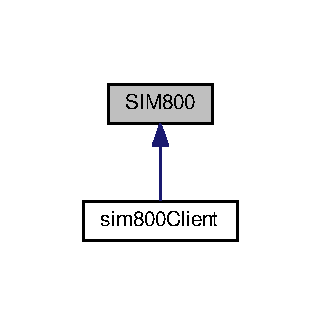
\includegraphics[width=154pt]{classSIM800__inherit__graph}
\end{center}
\end{figure}
\subsection*{Public Member Functions}
\begin{DoxyCompactItemize}
\item 
bool \hyperlink{classSIM800_aa021c75801b1918b5ad0fa56069f375c}{is\+On} ()
\begin{DoxyCompactList}\small\item\em Check if sim800 is on or is off. \end{DoxyCompactList}\item 
bool \hyperlink{classSIM800_ad582d1f567623255d8562a8fc01de236}{is\+Initialized} ()
\begin{DoxyCompactList}\small\item\em Check if sim800 is initialized. \end{DoxyCompactList}\item 
bool \hyperlink{classSIM800_a373c14a3362d291f32c8019f072dfe4e}{is\+Setted} ()
\begin{DoxyCompactList}\small\item\em Check if sim800 is setted. \end{DoxyCompactList}\item 
bool \hyperlink{classSIM800_a275fc00e4d607e244c3ce9f6eff032d2}{is\+Registered} ()
\begin{DoxyCompactList}\small\item\em Check if sim800 is registered on network. \end{DoxyCompactList}\item 
bool \hyperlink{classSIM800_aadbaa3d44c842c016d57c28bee6e1d1d}{is\+Http\+Initialized} ()
\begin{DoxyCompactList}\small\item\em Check if sim800 is connected. \end{DoxyCompactList}\item 
void \hyperlink{classSIM800_a4872e1f7377e73315966faff14c675d2}{set\+Serial} (Hardware\+Serial $\ast$serial)
\begin{DoxyCompactList}\small\item\em Set serial port for sim800. \end{DoxyCompactList}\item 
bool \hyperlink{classSIM800_aace0006eac0349e879e0b59395a86bc7}{init} (uint8\+\_\+t \+\_\+on\+\_\+off\+\_\+pin, uint8\+\_\+t \+\_\+reset\+\_\+pin=0x\+F\+F)
\begin{DoxyCompactList}\small\item\em Init variables for sim800. \end{DoxyCompactList}\item 
\hyperlink{sim800_8h_a3d1eeaa095df003ea28385b81a134b27}{sim800\+\_\+status\+\_\+t} \hyperlink{classSIM800_a9bbdd9fd81aaa798f6cc8ae9dfba0dce}{get\+Gsn} (char $\ast$imei)
\begin{DoxyCompactList}\small\item\em Send G\+SN AT command for reading simcard I\+M\+EI. \end{DoxyCompactList}\item 
\hyperlink{sim800_8h_a3d1eeaa095df003ea28385b81a134b27}{sim800\+\_\+status\+\_\+t} \hyperlink{classSIM800_acc33ebd53d7632af0231fe5762700a6c}{get\+Creg} (uint8\+\_\+t $\ast$n, uint8\+\_\+t $\ast$stat)
\begin{DoxyCompactList}\small\item\em Send C\+R\+EG AT command for reading network status. \end{DoxyCompactList}\item 
\hyperlink{sim800_8h_a3d1eeaa095df003ea28385b81a134b27}{sim800\+\_\+status\+\_\+t} \hyperlink{classSIM800_a4512a8ea233080900c43cc42fe8a4dfb}{get\+Csq} (uint8\+\_\+t $\ast$rssi, uint8\+\_\+t $\ast$ber)
\begin{DoxyCompactList}\small\item\em Send C\+SQ AT command for reading signal quality. \end{DoxyCompactList}\item 
\hyperlink{sim800_8h_a3d1eeaa095df003ea28385b81a134b27}{sim800\+\_\+status\+\_\+t} \hyperlink{classSIM800_a01c081285a1c61b068f97f06fb2004d9}{get\+Cgatt} (bool $\ast$is\+\_\+attached)
\begin{DoxyCompactList}\small\item\em Send C\+G\+A\+TT AT command for check if gprs is attached. \end{DoxyCompactList}\item 
\hyperlink{sim800_8h_a3d1eeaa095df003ea28385b81a134b27}{sim800\+\_\+status\+\_\+t} \hyperlink{classSIM800_a5313d75fb7510fe8b84b89def3b35096}{get\+Cifsr} (char $\ast$ip)
\begin{DoxyCompactList}\small\item\em Send C\+I\+F\+SR AT command for reading IP. \end{DoxyCompactList}\item 
\hyperlink{sim800_8h_a3d1eeaa095df003ea28385b81a134b27}{sim800\+\_\+status\+\_\+t} \hyperlink{classSIM800_ad8e19f34a392ac9b982fba48aed2d83e}{send\+Cpowd} ()
\begin{DoxyCompactList}\small\item\em Send C\+P\+O\+WD AT command for power off module. \end{DoxyCompactList}\item 
\hyperlink{sim800_8h_a3d1eeaa095df003ea28385b81a134b27}{sim800\+\_\+status\+\_\+t} \hyperlink{classSIM800_a30eb06e923b419efac4866dd630ae849}{switch\+On} ()
\begin{DoxyCompactList}\small\item\em Power on module. \end{DoxyCompactList}\item 
\hyperlink{sim800_8h_a3d1eeaa095df003ea28385b81a134b27}{sim800\+\_\+status\+\_\+t} \hyperlink{classSIM800_a6a7ee5f0c1ebaef0e04d3d0a8cb05032}{switch\+Off} (uint8\+\_\+t power\+\_\+off\+\_\+method=\hyperlink{sim800_8h_afec179273e643a34ac7e4991be4dfe7d}{S\+I\+M800\+\_\+\+P\+O\+W\+E\+R\+\_\+\+O\+F\+F\+\_\+\+B\+Y\+\_\+\+S\+W\+I\+T\+CH})
\begin{DoxyCompactList}\small\item\em Power off module. \end{DoxyCompactList}\item 
\hyperlink{sim800_8h_a3d1eeaa095df003ea28385b81a134b27}{sim800\+\_\+status\+\_\+t} \hyperlink{classSIM800_a05cceb142dd2e23b6459075f19c04ae8}{send\+At} ()
\begin{DoxyCompactList}\small\item\em Send \char`\"{}\+A\+T\char`\"{} AT command. \end{DoxyCompactList}\item 
\hyperlink{sim800_8h_a3d1eeaa095df003ea28385b81a134b27}{sim800\+\_\+status\+\_\+t} \hyperlink{classSIM800_ae2c0405faa73c05dd486b2a3f8086eb4}{init\+Autobaud} ()
\begin{DoxyCompactList}\small\item\em Execute autobaud sequence. \end{DoxyCompactList}\item 
\hyperlink{sim800_8h_a3d1eeaa095df003ea28385b81a134b27}{sim800\+\_\+status\+\_\+t} \hyperlink{classSIM800_af689d4460f01f57a910d4befc82b9b81}{setup} ()
\begin{DoxyCompactList}\small\item\em Execute setup sequence. \end{DoxyCompactList}\item 
\hyperlink{sim800_8h_a3d1eeaa095df003ea28385b81a134b27}{sim800\+\_\+status\+\_\+t} \hyperlink{classSIM800_aef7d718949e714a45d2f671fbd14e804}{start\+Connection} (const char $\ast$apn, const char $\ast$username, const char $\ast$password)
\begin{DoxyCompactList}\small\item\em Execute start connection sequence. \end{DoxyCompactList}\item 
\hyperlink{sim800_8h_a3d1eeaa095df003ea28385b81a134b27}{sim800\+\_\+status\+\_\+t} \hyperlink{classSIM800_a834bbcd0087d6f3ef3474b5914c39e3a}{connection} (const char $\ast$tipo, const char $\ast$server, const int port)
\begin{DoxyCompactList}\small\item\em Execute connection sequence. \end{DoxyCompactList}\item 
\hyperlink{sim800_8h_a3d1eeaa095df003ea28385b81a134b27}{sim800\+\_\+status\+\_\+t} \hyperlink{classSIM800_aac1e10bd21b00bfafc4487891a04e9d3}{stop\+Connection} ()
\begin{DoxyCompactList}\small\item\em Execute stop connection sequence. \end{DoxyCompactList}\item 
\hyperlink{sim800_8h_a3d1eeaa095df003ea28385b81a134b27}{sim800\+\_\+status\+\_\+t} \hyperlink{classSIM800_a3c73206225b81654384e625faadb1b49}{exit\+Transparent\+Mode} ()
\begin{DoxyCompactList}\small\item\em Execute exiting trasparent mode sequence. \end{DoxyCompactList}\item 
void \hyperlink{classSIM800_ad6ea4550521aee8f55656cede649baff}{clean\+Input} ()
\begin{DoxyCompactList}\small\item\em Clear read serial port stream. \end{DoxyCompactList}\item 
uint8\+\_\+t \hyperlink{classSIM800_a4dfa4237d627c04532156d476f29dacf}{receive} (char $\ast$rx\+\_\+buffer, const char $\ast$at\+\_\+ok\+\_\+string=\hyperlink{sim800_8h_a1da24009e90c1a5de1d1f0bc0dda6dc6}{A\+T\+\_\+\+O\+K\+\_\+\+S\+T\+R\+I\+NG}, const char $\ast$at\+\_\+error\+\_\+string=\hyperlink{sim800_8h_a883ea39010a33ca1b400940a65869e47}{A\+T\+\_\+\+E\+R\+R\+O\+R\+\_\+\+S\+T\+R\+I\+NG})
\begin{DoxyCompactList}\small\item\em Read serial port stream and check if response message is a success message or error message. \end{DoxyCompactList}\item 
\hyperlink{sim800_8h_a3d1eeaa095df003ea28385b81a134b27}{sim800\+\_\+status\+\_\+t} \hyperlink{classSIM800_a3ff02a2d318c230bc3711af6316a28c3}{send\+At\+Command} (const char $\ast$command, char $\ast$buf, const char $\ast$at\+\_\+ok\+\_\+string=\hyperlink{sim800_8h_a1da24009e90c1a5de1d1f0bc0dda6dc6}{A\+T\+\_\+\+O\+K\+\_\+\+S\+T\+R\+I\+NG}, const char $\ast$at\+\_\+error\+\_\+string=\hyperlink{sim800_8h_a883ea39010a33ca1b400940a65869e47}{A\+T\+\_\+\+E\+R\+R\+O\+R\+\_\+\+S\+T\+R\+I\+NG}, uint32\+\_\+t timeout\+\_\+ms=\hyperlink{sim800_8h_a0499ea42358376e7a0c09e540ab7219a}{S\+I\+M800\+\_\+\+A\+T\+\_\+\+D\+E\+F\+A\+U\+L\+T\+\_\+\+T\+I\+M\+E\+O\+U\+T\+\_\+\+MS})
\begin{DoxyCompactList}\small\item\em Write AT command to serial stream, managing timeout. \end{DoxyCompactList}\end{DoxyCompactItemize}
\subsection*{Public Attributes}
\begin{DoxyCompactItemize}
\item 
\mbox{\Hypertarget{classSIM800_a825f975081ae033934dca5404895246d}\label{classSIM800_a825f975081ae033934dca5404895246d}} 
uint8\+\_\+t \hyperlink{classSIM800_a825f975081ae033934dca5404895246d}{state}
\begin{DoxyCompactList}\small\item\em \hyperlink{classSIM800}{S\+I\+M800} state. \end{DoxyCompactList}\end{DoxyCompactItemize}
\subsection*{Protected Attributes}
\begin{DoxyCompactItemize}
\item 
\mbox{\Hypertarget{classSIM800_ac88d7703f4b6a439c4fb3a97bb0c5d0e}\label{classSIM800_ac88d7703f4b6a439c4fb3a97bb0c5d0e}} 
Hardware\+Serial $\ast$ \hyperlink{classSIM800_ac88d7703f4b6a439c4fb3a97bb0c5d0e}{modem} = \&Serial1
\begin{DoxyCompactList}\small\item\em pointer to modem serial stream. \end{DoxyCompactList}\end{DoxyCompactItemize}


\subsection{Detailed Description}
\hyperlink{classSIM800}{S\+I\+M800} class. 

\subsection{Member Function Documentation}
\mbox{\Hypertarget{classSIM800_ad6ea4550521aee8f55656cede649baff}\label{classSIM800_ad6ea4550521aee8f55656cede649baff}} 
\index{S\+I\+M800@{S\+I\+M800}!clean\+Input@{clean\+Input}}
\index{clean\+Input@{clean\+Input}!S\+I\+M800@{S\+I\+M800}}
\subsubsection{\texorpdfstring{clean\+Input()}{cleanInput()}}
{\footnotesize\ttfamily void S\+I\+M800\+::clean\+Input (\begin{DoxyParamCaption}{ }\end{DoxyParamCaption})}



Clear read serial port stream. 

\begin{DoxyReturn}{Returns}
void. 
\end{DoxyReturn}
\mbox{\Hypertarget{classSIM800_a834bbcd0087d6f3ef3474b5914c39e3a}\label{classSIM800_a834bbcd0087d6f3ef3474b5914c39e3a}} 
\index{S\+I\+M800@{S\+I\+M800}!connection@{connection}}
\index{connection@{connection}!S\+I\+M800@{S\+I\+M800}}
\subsubsection{\texorpdfstring{connection()}{connection()}}
{\footnotesize\ttfamily \hyperlink{sim800_8h_a3d1eeaa095df003ea28385b81a134b27}{sim800\+\_\+status\+\_\+t} S\+I\+M800\+::connection (\begin{DoxyParamCaption}\item[{const char $\ast$}]{tipo,  }\item[{const char $\ast$}]{server,  }\item[{const int}]{port }\end{DoxyParamCaption})}



Execute connection sequence. 


\begin{DoxyParams}[1]{Parameters}
\mbox{\tt in}  & {\em $\ast$tipo} & indicate what type of connection you want to open. Supported type are \char`\"{}\+U\+D\+P\char`\"{} and \char`\"{}\+T\+C\+P\char`\"{}. \\
\hline
\mbox{\tt in}  & {\em $\ast$server} & IP address or hostname of server. \\
\hline
\mbox{\tt in}  & {\em port} & connection port. \\
\hline
\end{DoxyParams}
\begin{DoxyReturn}{Returns}
sim800 status on each call. 
\end{DoxyReturn}
\mbox{\Hypertarget{classSIM800_a3c73206225b81654384e625faadb1b49}\label{classSIM800_a3c73206225b81654384e625faadb1b49}} 
\index{S\+I\+M800@{S\+I\+M800}!exit\+Transparent\+Mode@{exit\+Transparent\+Mode}}
\index{exit\+Transparent\+Mode@{exit\+Transparent\+Mode}!S\+I\+M800@{S\+I\+M800}}
\subsubsection{\texorpdfstring{exit\+Transparent\+Mode()}{exitTransparentMode()}}
{\footnotesize\ttfamily \hyperlink{sim800_8h_a3d1eeaa095df003ea28385b81a134b27}{sim800\+\_\+status\+\_\+t} S\+I\+M800\+::exit\+Transparent\+Mode (\begin{DoxyParamCaption}{ }\end{DoxyParamCaption})}



Execute exiting trasparent mode sequence. 

\begin{DoxyReturn}{Returns}
sim800 status on each call. 
\end{DoxyReturn}
\mbox{\Hypertarget{classSIM800_a01c081285a1c61b068f97f06fb2004d9}\label{classSIM800_a01c081285a1c61b068f97f06fb2004d9}} 
\index{S\+I\+M800@{S\+I\+M800}!get\+Cgatt@{get\+Cgatt}}
\index{get\+Cgatt@{get\+Cgatt}!S\+I\+M800@{S\+I\+M800}}
\subsubsection{\texorpdfstring{get\+Cgatt()}{getCgatt()}}
{\footnotesize\ttfamily \hyperlink{sim800_8h_a3d1eeaa095df003ea28385b81a134b27}{sim800\+\_\+status\+\_\+t} S\+I\+M800\+::get\+Cgatt (\begin{DoxyParamCaption}\item[{bool $\ast$}]{is\+\_\+attached }\end{DoxyParamCaption})}



Send C\+G\+A\+TT AT command for check if gprs is attached. 


\begin{DoxyParams}[1]{Parameters}
\mbox{\tt out}  & {\em $\ast$is\+\_\+attached} & pointer to bool variable indicating if gprs is attach (true) or not (false). \\
\hline
\end{DoxyParams}
\begin{DoxyReturn}{Returns}
sim800 status on each call. 
\end{DoxyReturn}
\mbox{\Hypertarget{classSIM800_a5313d75fb7510fe8b84b89def3b35096}\label{classSIM800_a5313d75fb7510fe8b84b89def3b35096}} 
\index{S\+I\+M800@{S\+I\+M800}!get\+Cifsr@{get\+Cifsr}}
\index{get\+Cifsr@{get\+Cifsr}!S\+I\+M800@{S\+I\+M800}}
\subsubsection{\texorpdfstring{get\+Cifsr()}{getCifsr()}}
{\footnotesize\ttfamily \hyperlink{sim800_8h_a3d1eeaa095df003ea28385b81a134b27}{sim800\+\_\+status\+\_\+t} S\+I\+M800\+::get\+Cifsr (\begin{DoxyParamCaption}\item[{char $\ast$}]{ip }\end{DoxyParamCaption})}



Send C\+I\+F\+SR AT command for reading IP. 


\begin{DoxyParams}[1]{Parameters}
\mbox{\tt out}  & {\em $\ast$ip} & pointer to char buffer containing ip. \\
\hline
\end{DoxyParams}
\begin{DoxyReturn}{Returns}
sim800 status on each call. 
\end{DoxyReturn}
\mbox{\Hypertarget{classSIM800_acc33ebd53d7632af0231fe5762700a6c}\label{classSIM800_acc33ebd53d7632af0231fe5762700a6c}} 
\index{S\+I\+M800@{S\+I\+M800}!get\+Creg@{get\+Creg}}
\index{get\+Creg@{get\+Creg}!S\+I\+M800@{S\+I\+M800}}
\subsubsection{\texorpdfstring{get\+Creg()}{getCreg()}}
{\footnotesize\ttfamily \hyperlink{sim800_8h_a3d1eeaa095df003ea28385b81a134b27}{sim800\+\_\+status\+\_\+t} S\+I\+M800\+::get\+Creg (\begin{DoxyParamCaption}\item[{uint8\+\_\+t $\ast$}]{n,  }\item[{uint8\+\_\+t $\ast$}]{stat }\end{DoxyParamCaption})}



Send C\+R\+EG AT command for reading network status. 


\begin{DoxyParams}[1]{Parameters}
\mbox{\tt out}  & {\em $\ast$n} & pointer to variable containing n value. \\
\hline
\mbox{\tt out}  & {\em $\ast$stat} & pointer to variable containing stat value. \\
\hline
\end{DoxyParams}
\begin{DoxyReturn}{Returns}
sim800 status on each call. 
\end{DoxyReturn}
\mbox{\Hypertarget{classSIM800_a4512a8ea233080900c43cc42fe8a4dfb}\label{classSIM800_a4512a8ea233080900c43cc42fe8a4dfb}} 
\index{S\+I\+M800@{S\+I\+M800}!get\+Csq@{get\+Csq}}
\index{get\+Csq@{get\+Csq}!S\+I\+M800@{S\+I\+M800}}
\subsubsection{\texorpdfstring{get\+Csq()}{getCsq()}}
{\footnotesize\ttfamily \hyperlink{sim800_8h_a3d1eeaa095df003ea28385b81a134b27}{sim800\+\_\+status\+\_\+t} S\+I\+M800\+::get\+Csq (\begin{DoxyParamCaption}\item[{uint8\+\_\+t $\ast$}]{rssi,  }\item[{uint8\+\_\+t $\ast$}]{ber }\end{DoxyParamCaption})}



Send C\+SQ AT command for reading signal quality. 


\begin{DoxyParams}[1]{Parameters}
\mbox{\tt out}  & {\em $\ast$rssi} & pointer to variable containing rssi value. \\
\hline
\mbox{\tt out}  & {\em $\ast$ber} & pointer to variable containing ber value. \\
\hline
\end{DoxyParams}
\begin{DoxyReturn}{Returns}
sim800 status on each call. 
\end{DoxyReturn}
\mbox{\Hypertarget{classSIM800_a9bbdd9fd81aaa798f6cc8ae9dfba0dce}\label{classSIM800_a9bbdd9fd81aaa798f6cc8ae9dfba0dce}} 
\index{S\+I\+M800@{S\+I\+M800}!get\+Gsn@{get\+Gsn}}
\index{get\+Gsn@{get\+Gsn}!S\+I\+M800@{S\+I\+M800}}
\subsubsection{\texorpdfstring{get\+Gsn()}{getGsn()}}
{\footnotesize\ttfamily \hyperlink{sim800_8h_a3d1eeaa095df003ea28385b81a134b27}{sim800\+\_\+status\+\_\+t} S\+I\+M800\+::get\+Gsn (\begin{DoxyParamCaption}\item[{char $\ast$}]{imei }\end{DoxyParamCaption})}



Send G\+SN AT command for reading simcard I\+M\+EI. 


\begin{DoxyParams}[1]{Parameters}
\mbox{\tt out}  & {\em $\ast$imei} & pointer to char buffer containing imei. \\
\hline
\end{DoxyParams}
\begin{DoxyReturn}{Returns}
sim800 status on each call. 
\end{DoxyReturn}
\mbox{\Hypertarget{classSIM800_aace0006eac0349e879e0b59395a86bc7}\label{classSIM800_aace0006eac0349e879e0b59395a86bc7}} 
\index{S\+I\+M800@{S\+I\+M800}!init@{init}}
\index{init@{init}!S\+I\+M800@{S\+I\+M800}}
\subsubsection{\texorpdfstring{init()}{init()}}
{\footnotesize\ttfamily bool S\+I\+M800\+::init (\begin{DoxyParamCaption}\item[{uint8\+\_\+t}]{\+\_\+on\+\_\+off\+\_\+pin,  }\item[{uint8\+\_\+t}]{\+\_\+reset\+\_\+pin = {\ttfamily 0xFF} }\end{DoxyParamCaption})}



Init variables for sim800. 


\begin{DoxyParams}[1]{Parameters}
\mbox{\tt in}  & {\em \+\_\+on\+\_\+off\+\_\+pin} & on/off pin for module. \\
\hline
\mbox{\tt in}  & {\em \+\_\+reset\+\_\+pin} & reset pin for module. \\
\hline
\end{DoxyParams}
\begin{DoxyReturn}{Returns}
true. 
\end{DoxyReturn}
\mbox{\Hypertarget{classSIM800_ae2c0405faa73c05dd486b2a3f8086eb4}\label{classSIM800_ae2c0405faa73c05dd486b2a3f8086eb4}} 
\index{S\+I\+M800@{S\+I\+M800}!init\+Autobaud@{init\+Autobaud}}
\index{init\+Autobaud@{init\+Autobaud}!S\+I\+M800@{S\+I\+M800}}
\subsubsection{\texorpdfstring{init\+Autobaud()}{initAutobaud()}}
{\footnotesize\ttfamily \hyperlink{sim800_8h_a3d1eeaa095df003ea28385b81a134b27}{sim800\+\_\+status\+\_\+t} S\+I\+M800\+::init\+Autobaud (\begin{DoxyParamCaption}{ }\end{DoxyParamCaption})}



Execute autobaud sequence. 

\begin{DoxyReturn}{Returns}
sim800 status on each call. 
\end{DoxyReturn}
\mbox{\Hypertarget{classSIM800_aadbaa3d44c842c016d57c28bee6e1d1d}\label{classSIM800_aadbaa3d44c842c016d57c28bee6e1d1d}} 
\index{S\+I\+M800@{S\+I\+M800}!is\+Http\+Initialized@{is\+Http\+Initialized}}
\index{is\+Http\+Initialized@{is\+Http\+Initialized}!S\+I\+M800@{S\+I\+M800}}
\subsubsection{\texorpdfstring{is\+Http\+Initialized()}{isHttpInitialized()}}
{\footnotesize\ttfamily bool S\+I\+M800\+::is\+Http\+Initialized (\begin{DoxyParamCaption}{ }\end{DoxyParamCaption})}



Check if sim800 is connected. 

\begin{DoxyReturn}{Returns}
true if it is connected, false otherwise. 
\end{DoxyReturn}
\mbox{\Hypertarget{classSIM800_ad582d1f567623255d8562a8fc01de236}\label{classSIM800_ad582d1f567623255d8562a8fc01de236}} 
\index{S\+I\+M800@{S\+I\+M800}!is\+Initialized@{is\+Initialized}}
\index{is\+Initialized@{is\+Initialized}!S\+I\+M800@{S\+I\+M800}}
\subsubsection{\texorpdfstring{is\+Initialized()}{isInitialized()}}
{\footnotesize\ttfamily bool S\+I\+M800\+::is\+Initialized (\begin{DoxyParamCaption}{ }\end{DoxyParamCaption})}



Check if sim800 is initialized. 

\begin{DoxyReturn}{Returns}
true if it is initialized, false otherwise. 
\end{DoxyReturn}
\mbox{\Hypertarget{classSIM800_aa021c75801b1918b5ad0fa56069f375c}\label{classSIM800_aa021c75801b1918b5ad0fa56069f375c}} 
\index{S\+I\+M800@{S\+I\+M800}!is\+On@{is\+On}}
\index{is\+On@{is\+On}!S\+I\+M800@{S\+I\+M800}}
\subsubsection{\texorpdfstring{is\+On()}{isOn()}}
{\footnotesize\ttfamily bool S\+I\+M800\+::is\+On (\begin{DoxyParamCaption}{ }\end{DoxyParamCaption})}



Check if sim800 is on or is off. 

\begin{DoxyReturn}{Returns}
true if it is on, false if is off. 
\end{DoxyReturn}
\mbox{\Hypertarget{classSIM800_a275fc00e4d607e244c3ce9f6eff032d2}\label{classSIM800_a275fc00e4d607e244c3ce9f6eff032d2}} 
\index{S\+I\+M800@{S\+I\+M800}!is\+Registered@{is\+Registered}}
\index{is\+Registered@{is\+Registered}!S\+I\+M800@{S\+I\+M800}}
\subsubsection{\texorpdfstring{is\+Registered()}{isRegistered()}}
{\footnotesize\ttfamily bool S\+I\+M800\+::is\+Registered (\begin{DoxyParamCaption}{ }\end{DoxyParamCaption})}



Check if sim800 is registered on network. 

\begin{DoxyReturn}{Returns}
true if it is registered, false otherwise. 
\end{DoxyReturn}
\mbox{\Hypertarget{classSIM800_a373c14a3362d291f32c8019f072dfe4e}\label{classSIM800_a373c14a3362d291f32c8019f072dfe4e}} 
\index{S\+I\+M800@{S\+I\+M800}!is\+Setted@{is\+Setted}}
\index{is\+Setted@{is\+Setted}!S\+I\+M800@{S\+I\+M800}}
\subsubsection{\texorpdfstring{is\+Setted()}{isSetted()}}
{\footnotesize\ttfamily bool S\+I\+M800\+::is\+Setted (\begin{DoxyParamCaption}{ }\end{DoxyParamCaption})}



Check if sim800 is setted. 

\begin{DoxyReturn}{Returns}
true if it is setted, false otherwise. 
\end{DoxyReturn}
\mbox{\Hypertarget{classSIM800_a4dfa4237d627c04532156d476f29dacf}\label{classSIM800_a4dfa4237d627c04532156d476f29dacf}} 
\index{S\+I\+M800@{S\+I\+M800}!receive@{receive}}
\index{receive@{receive}!S\+I\+M800@{S\+I\+M800}}
\subsubsection{\texorpdfstring{receive()}{receive()}}
{\footnotesize\ttfamily uint8\+\_\+t S\+I\+M800\+::receive (\begin{DoxyParamCaption}\item[{char $\ast$}]{rx\+\_\+buffer,  }\item[{const char $\ast$}]{at\+\_\+ok\+\_\+string = {\ttfamily \hyperlink{sim800_8h_a1da24009e90c1a5de1d1f0bc0dda6dc6}{A\+T\+\_\+\+O\+K\+\_\+\+S\+T\+R\+I\+NG}},  }\item[{const char $\ast$}]{at\+\_\+error\+\_\+string = {\ttfamily \hyperlink{sim800_8h_a883ea39010a33ca1b400940a65869e47}{A\+T\+\_\+\+E\+R\+R\+O\+R\+\_\+\+S\+T\+R\+I\+NG}} }\end{DoxyParamCaption})}



Read serial port stream and check if response message is a success message or error message. 


\begin{DoxyParams}[1]{Parameters}
\mbox{\tt out}  & {\em $\ast$rx\+\_\+buffer} & pointer to readed data buffer. \\
\hline
\mbox{\tt in}  & {\em $\ast$at\+\_\+ok\+\_\+string} & success message. \\
\hline
\mbox{\tt in}  & {\em $\ast$at\+\_\+error\+\_\+string} & error message. \\
\hline
\end{DoxyParams}
\begin{DoxyReturn}{Returns}
number of bytes readed from stream. 
\end{DoxyReturn}
\mbox{\Hypertarget{classSIM800_a05cceb142dd2e23b6459075f19c04ae8}\label{classSIM800_a05cceb142dd2e23b6459075f19c04ae8}} 
\index{S\+I\+M800@{S\+I\+M800}!send\+At@{send\+At}}
\index{send\+At@{send\+At}!S\+I\+M800@{S\+I\+M800}}
\subsubsection{\texorpdfstring{send\+At()}{sendAt()}}
{\footnotesize\ttfamily \hyperlink{sim800_8h_a3d1eeaa095df003ea28385b81a134b27}{sim800\+\_\+status\+\_\+t} S\+I\+M800\+::send\+At (\begin{DoxyParamCaption}{ }\end{DoxyParamCaption})}



Send \char`\"{}\+A\+T\char`\"{} AT command. 

\begin{DoxyReturn}{Returns}
sim800 status. 
\end{DoxyReturn}
\mbox{\Hypertarget{classSIM800_a3ff02a2d318c230bc3711af6316a28c3}\label{classSIM800_a3ff02a2d318c230bc3711af6316a28c3}} 
\index{S\+I\+M800@{S\+I\+M800}!send\+At\+Command@{send\+At\+Command}}
\index{send\+At\+Command@{send\+At\+Command}!S\+I\+M800@{S\+I\+M800}}
\subsubsection{\texorpdfstring{send\+At\+Command()}{sendAtCommand()}}
{\footnotesize\ttfamily S\+I\+M800\+::send\+At\+Command (\begin{DoxyParamCaption}\item[{const char $\ast$}]{command,  }\item[{char $\ast$}]{buf,  }\item[{const char $\ast$}]{at\+\_\+ok\+\_\+string = {\ttfamily \hyperlink{sim800_8h_a1da24009e90c1a5de1d1f0bc0dda6dc6}{A\+T\+\_\+\+O\+K\+\_\+\+S\+T\+R\+I\+NG}},  }\item[{const char $\ast$}]{at\+\_\+error\+\_\+string = {\ttfamily \hyperlink{sim800_8h_a883ea39010a33ca1b400940a65869e47}{A\+T\+\_\+\+E\+R\+R\+O\+R\+\_\+\+S\+T\+R\+I\+NG}},  }\item[{uint32\+\_\+t}]{timeout\+\_\+ms = {\ttfamily \hyperlink{sim800_8h_a0499ea42358376e7a0c09e540ab7219a}{S\+I\+M800\+\_\+\+A\+T\+\_\+\+D\+E\+F\+A\+U\+L\+T\+\_\+\+T\+I\+M\+E\+O\+U\+T\+\_\+\+MS}} }\end{DoxyParamCaption})}



Write AT command to serial stream, managing timeout. 


\begin{DoxyParams}[1]{Parameters}
\mbox{\tt in}  & {\em $\ast$command} & AT command to be send. \\
\hline
\mbox{\tt in,out}  & {\em $\ast$buf} & pointer to readed and writed data buffer. \\
\hline
\mbox{\tt in}  & {\em $\ast$at\+\_\+ok\+\_\+string} & success message. \\
\hline
\mbox{\tt in}  & {\em $\ast$at\+\_\+error\+\_\+string} & error message. \\
\hline
\mbox{\tt in}  & {\em timeout\+\_\+ms} & timeout in milliseconds for receive a response. \\
\hline
\end{DoxyParams}
\begin{DoxyReturn}{Returns}
sim800 status on each call. 
\end{DoxyReturn}
\mbox{\Hypertarget{classSIM800_ad8e19f34a392ac9b982fba48aed2d83e}\label{classSIM800_ad8e19f34a392ac9b982fba48aed2d83e}} 
\index{S\+I\+M800@{S\+I\+M800}!send\+Cpowd@{send\+Cpowd}}
\index{send\+Cpowd@{send\+Cpowd}!S\+I\+M800@{S\+I\+M800}}
\subsubsection{\texorpdfstring{send\+Cpowd()}{sendCpowd()}}
{\footnotesize\ttfamily \hyperlink{sim800_8h_a3d1eeaa095df003ea28385b81a134b27}{sim800\+\_\+status\+\_\+t} S\+I\+M800\+::send\+Cpowd (\begin{DoxyParamCaption}{ }\end{DoxyParamCaption})}



Send C\+P\+O\+WD AT command for power off module. 

\begin{DoxyReturn}{Returns}
sim800 status on each call. 
\end{DoxyReturn}
\mbox{\Hypertarget{classSIM800_a4872e1f7377e73315966faff14c675d2}\label{classSIM800_a4872e1f7377e73315966faff14c675d2}} 
\index{S\+I\+M800@{S\+I\+M800}!set\+Serial@{set\+Serial}}
\index{set\+Serial@{set\+Serial}!S\+I\+M800@{S\+I\+M800}}
\subsubsection{\texorpdfstring{set\+Serial()}{setSerial()}}
{\footnotesize\ttfamily void S\+I\+M800\+::set\+Serial (\begin{DoxyParamCaption}\item[{Hardware\+Serial $\ast$}]{serial }\end{DoxyParamCaption})}



Set serial port for sim800. 


\begin{DoxyParams}[1]{Parameters}
\mbox{\tt in}  & {\em $\ast$serial} & pointer to serial stream. \\
\hline
\end{DoxyParams}
\begin{DoxyReturn}{Returns}
void. 
\end{DoxyReturn}
\mbox{\Hypertarget{classSIM800_af689d4460f01f57a910d4befc82b9b81}\label{classSIM800_af689d4460f01f57a910d4befc82b9b81}} 
\index{S\+I\+M800@{S\+I\+M800}!setup@{setup}}
\index{setup@{setup}!S\+I\+M800@{S\+I\+M800}}
\subsubsection{\texorpdfstring{setup()}{setup()}}
{\footnotesize\ttfamily \hyperlink{sim800_8h_a3d1eeaa095df003ea28385b81a134b27}{sim800\+\_\+status\+\_\+t} S\+I\+M800\+::setup (\begin{DoxyParamCaption}{ }\end{DoxyParamCaption})}



Execute setup sequence. 

\begin{DoxyReturn}{Returns}
sim800 status on each call. 
\end{DoxyReturn}
\mbox{\Hypertarget{classSIM800_aef7d718949e714a45d2f671fbd14e804}\label{classSIM800_aef7d718949e714a45d2f671fbd14e804}} 
\index{S\+I\+M800@{S\+I\+M800}!start\+Connection@{start\+Connection}}
\index{start\+Connection@{start\+Connection}!S\+I\+M800@{S\+I\+M800}}
\subsubsection{\texorpdfstring{start\+Connection()}{startConnection()}}
{\footnotesize\ttfamily \hyperlink{sim800_8h_a3d1eeaa095df003ea28385b81a134b27}{sim800\+\_\+status\+\_\+t} S\+I\+M800\+::start\+Connection (\begin{DoxyParamCaption}\item[{const char $\ast$}]{apn,  }\item[{const char $\ast$}]{username,  }\item[{const char $\ast$}]{password }\end{DoxyParamCaption})}



Execute start connection sequence. 


\begin{DoxyParams}[1]{Parameters}
\mbox{\tt in}  & {\em $\ast$apn} & apn for simcard network operation \\
\hline
\mbox{\tt in}  & {\em $\ast$username} & username for simcard network operation \\
\hline
\mbox{\tt in}  & {\em $\ast$password} & password for simcard network operation \\
\hline
\end{DoxyParams}
\begin{DoxyReturn}{Returns}
sim800 status on each call. 
\end{DoxyReturn}
\mbox{\Hypertarget{classSIM800_aac1e10bd21b00bfafc4487891a04e9d3}\label{classSIM800_aac1e10bd21b00bfafc4487891a04e9d3}} 
\index{S\+I\+M800@{S\+I\+M800}!stop\+Connection@{stop\+Connection}}
\index{stop\+Connection@{stop\+Connection}!S\+I\+M800@{S\+I\+M800}}
\subsubsection{\texorpdfstring{stop\+Connection()}{stopConnection()}}
{\footnotesize\ttfamily \hyperlink{sim800_8h_a3d1eeaa095df003ea28385b81a134b27}{sim800\+\_\+status\+\_\+t} S\+I\+M800\+::stop\+Connection (\begin{DoxyParamCaption}{ }\end{DoxyParamCaption})}



Execute stop connection sequence. 

\begin{DoxyReturn}{Returns}
sim800 status on each call. 
\end{DoxyReturn}
\mbox{\Hypertarget{classSIM800_a6a7ee5f0c1ebaef0e04d3d0a8cb05032}\label{classSIM800_a6a7ee5f0c1ebaef0e04d3d0a8cb05032}} 
\index{S\+I\+M800@{S\+I\+M800}!switch\+Off@{switch\+Off}}
\index{switch\+Off@{switch\+Off}!S\+I\+M800@{S\+I\+M800}}
\subsubsection{\texorpdfstring{switch\+Off()}{switchOff()}}
{\footnotesize\ttfamily \hyperlink{sim800_8h_a3d1eeaa095df003ea28385b81a134b27}{sim800\+\_\+status\+\_\+t} S\+I\+M800\+::switch\+Off (\begin{DoxyParamCaption}\item[{uint8\+\_\+t}]{power\+\_\+off\+\_\+method = {\ttfamily \hyperlink{sim800_8h_afec179273e643a34ac7e4991be4dfe7d}{S\+I\+M800\+\_\+\+P\+O\+W\+E\+R\+\_\+\+O\+F\+F\+\_\+\+B\+Y\+\_\+\+S\+W\+I\+T\+CH}} }\end{DoxyParamCaption})}



Power off module. 


\begin{DoxyParams}[1]{Parameters}
\mbox{\tt in}  & {\em power\+\_\+off\+\_\+method} & indicate what method you want to use for power off module (hardware switch or AT command). Default is hardware switch. \\
\hline
\end{DoxyParams}
\begin{DoxyReturn}{Returns}
sim800 status on each call. 
\end{DoxyReturn}
\mbox{\Hypertarget{classSIM800_a30eb06e923b419efac4866dd630ae849}\label{classSIM800_a30eb06e923b419efac4866dd630ae849}} 
\index{S\+I\+M800@{S\+I\+M800}!switch\+On@{switch\+On}}
\index{switch\+On@{switch\+On}!S\+I\+M800@{S\+I\+M800}}
\subsubsection{\texorpdfstring{switch\+On()}{switchOn()}}
{\footnotesize\ttfamily \hyperlink{sim800_8h_a3d1eeaa095df003ea28385b81a134b27}{sim800\+\_\+status\+\_\+t} S\+I\+M800\+::switch\+On (\begin{DoxyParamCaption}{ }\end{DoxyParamCaption})}



Power on module. 

\begin{DoxyReturn}{Returns}
sim800 status on each call. 
\end{DoxyReturn}


The documentation for this class was generated from the following files\+:\begin{DoxyCompactItemize}
\item 
sketchbook/libraries/sim800/\hyperlink{sim800_8h}{sim800.\+h}\item 
sketchbook/libraries/sim800/\hyperlink{sim800_8cpp}{sim800.\+cpp}\end{DoxyCompactItemize}

\hypertarget{classsim800Client}{}\section{sim800\+Client Class Reference}
\label{classsim800Client}\index{sim800\+Client@{sim800\+Client}}


\hyperlink{classsim800Client}{sim800\+Client} class.  




{\ttfamily \#include $<$sim800\+Client.\+h$>$}



Inheritance diagram for sim800\+Client\+:\nopagebreak
\begin{figure}[H]
\begin{center}
\leavevmode
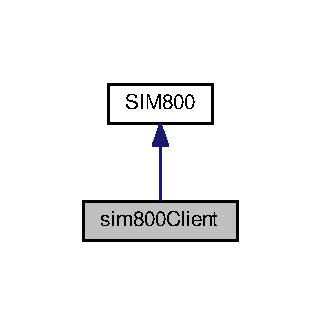
\includegraphics[width=154pt]{classsim800Client__inherit__graph}
\end{center}
\end{figure}


Collaboration diagram for sim800\+Client\+:\nopagebreak
\begin{figure}[H]
\begin{center}
\leavevmode
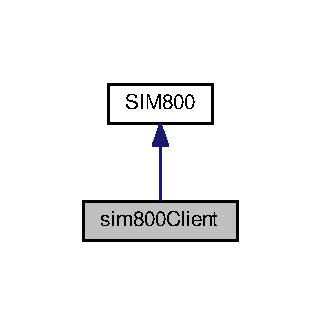
\includegraphics[width=154pt]{classsim800Client__coll__graph}
\end{center}
\end{figure}
\subsection*{Public Member Functions}
\begin{DoxyCompactItemize}
\item 
int \hyperlink{classsim800Client_a2c26282b71132af7f50becb62d9fe0f4}{connect} (I\+P\+Address ip, int port)
\begin{DoxyCompactList}\small\item\em Connect to server at specified port. \end{DoxyCompactList}\item 
int \hyperlink{classsim800Client_ae74b00f32682498c63b05dd615705ea7}{connect} (const char $\ast$host, int port)
\begin{DoxyCompactList}\small\item\em Connect to server at specified port. \end{DoxyCompactList}\item 
uint8\+\_\+t \hyperlink{classsim800Client_ad3a5903a0f8c264ec445edafe167f4f0}{connected} ()
\begin{DoxyCompactList}\small\item\em Check if connection was performed. \end{DoxyCompactList}\item 
int \hyperlink{classsim800Client_ae6648c39586919bddcc5c1d24f395767}{available} ()
\begin{DoxyCompactList}\small\item\em Return the number of bytes available in the stream. \end{DoxyCompactList}\item 
int \hyperlink{classsim800Client_adafda98d2cc49e401053b3ba521d49b4}{read} ()
\begin{DoxyCompactList}\small\item\em Reads one characters from an incoming stream. \end{DoxyCompactList}\item 
int \hyperlink{classsim800Client_ac200fe43c977c3b6f981b07206ea0e4c}{read\+Bytes} (char $\ast$buffer, size\+\_\+t size)
\begin{DoxyCompactList}\small\item\em Read characters from a stream into a buffer. Terminates if the determined length has been read, or it times out. \end{DoxyCompactList}\item 
int \hyperlink{classsim800Client_a961a22382e23d4ce928a60098cc13973}{read\+Bytes} (uint8\+\_\+t $\ast$buffer, size\+\_\+t size)
\begin{DoxyCompactList}\small\item\em Read bytes from a stream into a buffer. Terminates if the determined length has been read, or it times out. \end{DoxyCompactList}\item 
void \hyperlink{classsim800Client_a10001f737f1331303472de45a2d8faa1}{set\+Timeout} (uint32\+\_\+t timeout)
\begin{DoxyCompactList}\small\item\em Sets the maximum milliseconds to wait for stream data. \end{DoxyCompactList}\item 
size\+\_\+t \hyperlink{classsim800Client_ab730edb73267508cbc261b13e643b12d}{write} (uint8\+\_\+t buffer)
\begin{DoxyCompactList}\small\item\em Write bytes from a buffer into a stream. \end{DoxyCompactList}\item 
size\+\_\+t \hyperlink{classsim800Client_aef786fd9fa179f04b016c7cb916a7f39}{write} (const uint8\+\_\+t $\ast$buffer, size\+\_\+t size)
\begin{DoxyCompactList}\small\item\em Write bytes from a buffer into a stream. Terminates if the determined length has been written. \end{DoxyCompactList}\item 
void \hyperlink{classsim800Client_a2d7b70eec8e0ff108b3c3fee4eb9b559}{flush} ()
\begin{DoxyCompactList}\small\item\em Clears the buffer once all outgoing characters have been sent. \end{DoxyCompactList}\item 
void \hyperlink{classsim800Client_a26d88d095ba02c26e5d5dd8ba22e01c0}{stop} ()
\begin{DoxyCompactList}\small\item\em Stop. \end{DoxyCompactList}\end{DoxyCompactItemize}
\subsection*{Additional Inherited Members}


\subsection{Detailed Description}
\hyperlink{classsim800Client}{sim800\+Client} class. 

\subsection{Member Function Documentation}
\mbox{\Hypertarget{classsim800Client_ae6648c39586919bddcc5c1d24f395767}\label{classsim800Client_ae6648c39586919bddcc5c1d24f395767}} 
\index{sim800\+Client@{sim800\+Client}!available@{available}}
\index{available@{available}!sim800\+Client@{sim800\+Client}}
\subsubsection{\texorpdfstring{available()}{available()}}
{\footnotesize\ttfamily int sim800\+Client\+::available (\begin{DoxyParamCaption}{ }\end{DoxyParamCaption})}



Return the number of bytes available in the stream. 

\begin{DoxyReturn}{Returns}
the number of bytes available. 
\end{DoxyReturn}
\mbox{\Hypertarget{classsim800Client_a2c26282b71132af7f50becb62d9fe0f4}\label{classsim800Client_a2c26282b71132af7f50becb62d9fe0f4}} 
\index{sim800\+Client@{sim800\+Client}!connect@{connect}}
\index{connect@{connect}!sim800\+Client@{sim800\+Client}}
\subsubsection{\texorpdfstring{connect()}{connect()}\hspace{0.1cm}{\footnotesize\ttfamily [1/2]}}
{\footnotesize\ttfamily int sim800\+Client\+::connect (\begin{DoxyParamCaption}\item[{I\+P\+Address}]{ip,  }\item[{int}]{port }\end{DoxyParamCaption})}



Connect to server at specified port. 


\begin{DoxyParams}[1]{Parameters}
\mbox{\tt in}  & {\em ip} & ip address of server. \\
\hline
\mbox{\tt in}  & {\em port} & port to server. \\
\hline
\end{DoxyParams}
\begin{DoxyReturn}{Returns}
sim800 status of connection sequence on each call. 
\end{DoxyReturn}
\mbox{\Hypertarget{classsim800Client_ae74b00f32682498c63b05dd615705ea7}\label{classsim800Client_ae74b00f32682498c63b05dd615705ea7}} 
\index{sim800\+Client@{sim800\+Client}!connect@{connect}}
\index{connect@{connect}!sim800\+Client@{sim800\+Client}}
\subsubsection{\texorpdfstring{connect()}{connect()}\hspace{0.1cm}{\footnotesize\ttfamily [2/2]}}
{\footnotesize\ttfamily int sim800\+Client\+::connect (\begin{DoxyParamCaption}\item[{const char $\ast$}]{host,  }\item[{int}]{port }\end{DoxyParamCaption})}



Connect to server at specified port. 


\begin{DoxyParams}[1]{Parameters}
\mbox{\tt in}  & {\em $\ast$host} & hostname of server. \\
\hline
\mbox{\tt in}  & {\em port} & port to server. \\
\hline
\end{DoxyParams}
\begin{DoxyReturn}{Returns}
sim800 status of connection sequence on each call. 
\end{DoxyReturn}
\mbox{\Hypertarget{classsim800Client_ad3a5903a0f8c264ec445edafe167f4f0}\label{classsim800Client_ad3a5903a0f8c264ec445edafe167f4f0}} 
\index{sim800\+Client@{sim800\+Client}!connected@{connected}}
\index{connected@{connected}!sim800\+Client@{sim800\+Client}}
\subsubsection{\texorpdfstring{connected()}{connected()}}
{\footnotesize\ttfamily uint8\+\_\+t sim800\+Client\+::connected (\begin{DoxyParamCaption}{ }\end{DoxyParamCaption})}



Check if connection was performed. 

\begin{DoxyReturn}{Returns}
true if it is connected, false otherwise. 
\end{DoxyReturn}
\mbox{\Hypertarget{classsim800Client_a2d7b70eec8e0ff108b3c3fee4eb9b559}\label{classsim800Client_a2d7b70eec8e0ff108b3c3fee4eb9b559}} 
\index{sim800\+Client@{sim800\+Client}!flush@{flush}}
\index{flush@{flush}!sim800\+Client@{sim800\+Client}}
\subsubsection{\texorpdfstring{flush()}{flush()}}
{\footnotesize\ttfamily void sim800\+Client\+::flush (\begin{DoxyParamCaption}{ }\end{DoxyParamCaption})}



Clears the buffer once all outgoing characters have been sent. 

\begin{DoxyReturn}{Returns}
void. 
\end{DoxyReturn}
\mbox{\Hypertarget{classsim800Client_adafda98d2cc49e401053b3ba521d49b4}\label{classsim800Client_adafda98d2cc49e401053b3ba521d49b4}} 
\index{sim800\+Client@{sim800\+Client}!read@{read}}
\index{read@{read}!sim800\+Client@{sim800\+Client}}
\subsubsection{\texorpdfstring{read()}{read()}}
{\footnotesize\ttfamily int sim800\+Client\+::read (\begin{DoxyParamCaption}{ }\end{DoxyParamCaption})}



Reads one characters from an incoming stream. 

\begin{DoxyReturn}{Returns}
The readed characters or -\/1 if there isn\textquotesingle{}t characters. 
\end{DoxyReturn}
\mbox{\Hypertarget{classsim800Client_ac200fe43c977c3b6f981b07206ea0e4c}\label{classsim800Client_ac200fe43c977c3b6f981b07206ea0e4c}} 
\index{sim800\+Client@{sim800\+Client}!read\+Bytes@{read\+Bytes}}
\index{read\+Bytes@{read\+Bytes}!sim800\+Client@{sim800\+Client}}
\subsubsection{\texorpdfstring{read\+Bytes()}{readBytes()}\hspace{0.1cm}{\footnotesize\ttfamily [1/2]}}
{\footnotesize\ttfamily int sim800\+Client\+::read\+Bytes (\begin{DoxyParamCaption}\item[{char $\ast$}]{buffer,  }\item[{size\+\_\+t}]{size }\end{DoxyParamCaption})}



Read characters from a stream into a buffer. Terminates if the determined length has been read, or it times out. 


\begin{DoxyParams}[1]{Parameters}
\mbox{\tt out}  & {\em $\ast$buffer} & pointer to readed characters buffer. \\
\hline
\mbox{\tt in}  & {\em size} & maximum number of characters to be read. \\
\hline
\end{DoxyParams}
\begin{DoxyReturn}{Returns}
the number of characters placed in the buffer. A 0 means no valid data was found. 
\end{DoxyReturn}
\mbox{\Hypertarget{classsim800Client_a961a22382e23d4ce928a60098cc13973}\label{classsim800Client_a961a22382e23d4ce928a60098cc13973}} 
\index{sim800\+Client@{sim800\+Client}!read\+Bytes@{read\+Bytes}}
\index{read\+Bytes@{read\+Bytes}!sim800\+Client@{sim800\+Client}}
\subsubsection{\texorpdfstring{read\+Bytes()}{readBytes()}\hspace{0.1cm}{\footnotesize\ttfamily [2/2]}}
{\footnotesize\ttfamily int sim800\+Client\+::read\+Bytes (\begin{DoxyParamCaption}\item[{uint8\+\_\+t $\ast$}]{buffer,  }\item[{size\+\_\+t}]{size }\end{DoxyParamCaption})}



Read bytes from a stream into a buffer. Terminates if the determined length has been read, or it times out. 


\begin{DoxyParams}[1]{Parameters}
\mbox{\tt out}  & {\em $\ast$buffer} & pointer to readed bytes buffer. \\
\hline
\mbox{\tt in}  & {\em size} & maximum number of bytes to be read. \\
\hline
\end{DoxyParams}
\begin{DoxyReturn}{Returns}
the number of bytes placed in the buffer. A 0 means no valid data was found. 
\end{DoxyReturn}
\mbox{\Hypertarget{classsim800Client_a10001f737f1331303472de45a2d8faa1}\label{classsim800Client_a10001f737f1331303472de45a2d8faa1}} 
\index{sim800\+Client@{sim800\+Client}!set\+Timeout@{set\+Timeout}}
\index{set\+Timeout@{set\+Timeout}!sim800\+Client@{sim800\+Client}}
\subsubsection{\texorpdfstring{set\+Timeout()}{setTimeout()}}
{\footnotesize\ttfamily void sim800\+Client\+::set\+Timeout (\begin{DoxyParamCaption}\item[{uint32\+\_\+t}]{timeout }\end{DoxyParamCaption})}



Sets the maximum milliseconds to wait for stream data. 


\begin{DoxyParams}[1]{Parameters}
\mbox{\tt in}  & {\em timeout} & milliseconds for timeout. \\
\hline
\end{DoxyParams}
\begin{DoxyReturn}{Returns}
void. 
\end{DoxyReturn}
\mbox{\Hypertarget{classsim800Client_a26d88d095ba02c26e5d5dd8ba22e01c0}\label{classsim800Client_a26d88d095ba02c26e5d5dd8ba22e01c0}} 
\index{sim800\+Client@{sim800\+Client}!stop@{stop}}
\index{stop@{stop}!sim800\+Client@{sim800\+Client}}
\subsubsection{\texorpdfstring{stop()}{stop()}}
{\footnotesize\ttfamily void sim800\+Client\+::stop (\begin{DoxyParamCaption}{ }\end{DoxyParamCaption})}



Stop. 

\begin{DoxyReturn}{Returns}
void. 
\end{DoxyReturn}
\mbox{\Hypertarget{classsim800Client_ab730edb73267508cbc261b13e643b12d}\label{classsim800Client_ab730edb73267508cbc261b13e643b12d}} 
\index{sim800\+Client@{sim800\+Client}!write@{write}}
\index{write@{write}!sim800\+Client@{sim800\+Client}}
\subsubsection{\texorpdfstring{write()}{write()}\hspace{0.1cm}{\footnotesize\ttfamily [1/2]}}
{\footnotesize\ttfamily size\+\_\+t sim800\+Client\+::write (\begin{DoxyParamCaption}\item[{uint8\+\_\+t}]{buffer }\end{DoxyParamCaption})}



Write bytes from a buffer into a stream. 


\begin{DoxyParams}[1]{Parameters}
\mbox{\tt in}  & {\em $\ast$buffer} & pointer to write bytes buffer. \\
\hline
\end{DoxyParams}
\begin{DoxyReturn}{Returns}
the number of bytes written in the buffer. 
\end{DoxyReturn}
\mbox{\Hypertarget{classsim800Client_aef786fd9fa179f04b016c7cb916a7f39}\label{classsim800Client_aef786fd9fa179f04b016c7cb916a7f39}} 
\index{sim800\+Client@{sim800\+Client}!write@{write}}
\index{write@{write}!sim800\+Client@{sim800\+Client}}
\subsubsection{\texorpdfstring{write()}{write()}\hspace{0.1cm}{\footnotesize\ttfamily [2/2]}}
{\footnotesize\ttfamily size\+\_\+t sim800\+Client\+::write (\begin{DoxyParamCaption}\item[{const uint8\+\_\+t $\ast$}]{buffer,  }\item[{size\+\_\+t}]{size }\end{DoxyParamCaption})}



Write bytes from a buffer into a stream. Terminates if the determined length has been written. 


\begin{DoxyParams}[1]{Parameters}
\mbox{\tt in}  & {\em $\ast$buffer} & pointer to write bytes buffer. \\
\hline
\mbox{\tt in}  & {\em size} & maximum number of bytes to write into stream. \\
\hline
\end{DoxyParams}
\begin{DoxyReturn}{Returns}
the number of bytes written in the buffer. 
\end{DoxyReturn}


The documentation for this class was generated from the following files\+:\begin{DoxyCompactItemize}
\item 
sketchbook/libraries/sim800/\hyperlink{sim800Client_8h}{sim800\+Client.\+h}\item 
sketchbook/libraries/sim800/\hyperlink{sim800_8cpp}{sim800.\+cpp}\end{DoxyCompactItemize}

\input{structvalue__t}
\input{structwritable__data__t}
\chapter{File Documentation}
\hypertarget{digiteco__power_8cpp}{}\section{sketchbook/libraries/\+Digiteco\+Power/digiteco\+\_\+power.cpp File Reference}
\label{digiteco__power_8cpp}\index{sketchbook/libraries/\+Digiteco\+Power/digiteco\+\_\+power.\+cpp@{sketchbook/libraries/\+Digiteco\+Power/digiteco\+\_\+power.\+cpp}}
{\ttfamily \#include \char`\"{}digiteco\+\_\+power.\+h\char`\"{}}\newline
Include dependency graph for digiteco\+\_\+power.\+cpp\+:\nopagebreak
\begin{figure}[H]
\begin{center}
\leavevmode
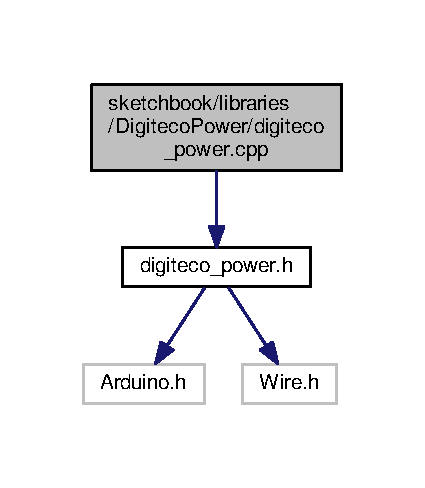
\includegraphics[width=204pt]{digiteco__power_8cpp__incl}
\end{center}
\end{figure}
\subsection*{Namespaces}
\begin{DoxyCompactItemize}
\item 
 \hyperlink{namespaceDigitecoPower}{Digiteco\+Power}
\begin{DoxyCompactList}\small\item\em \hyperlink{namespaceDigitecoPower}{Digiteco\+Power} namespace. \end{DoxyCompactList}\end{DoxyCompactItemize}
\subsection*{Functions}
\begin{DoxyCompactItemize}
\item 
bool \hyperlink{namespaceDigitecoPower_adb7461d6d597526eace685d0365732b7}{Digiteco\+Power\+::de\+\_\+read} (uint8\+\_\+t address, float $\ast$value)
\begin{DoxyCompactList}\small\item\em Read value at specified i2c-\/address. \end{DoxyCompactList}\item 
bool \hyperlink{namespaceDigitecoPower_a2a1d64ce6df863e91fef034a496220fd}{Digiteco\+Power\+::de\+\_\+send} (uint8\+\_\+t address, uint8\+\_\+t data)
\begin{DoxyCompactList}\small\item\em Send data at specified i2c-\/address. \end{DoxyCompactList}\end{DoxyCompactItemize}

\hypertarget{digiteco__power_8h}{}\section{sketchbook/libraries/\+Digiteco\+Power/digiteco\+\_\+power.h File Reference}
\label{digiteco__power_8h}\index{sketchbook/libraries/\+Digiteco\+Power/digiteco\+\_\+power.\+h@{sketchbook/libraries/\+Digiteco\+Power/digiteco\+\_\+power.\+h}}
{\ttfamily \#include $<$Arduino.\+h$>$}\newline
{\ttfamily \#include $<$Wire.\+h$>$}\newline
Include dependency graph for digiteco\+\_\+power.\+h\+:\nopagebreak
\begin{figure}[H]
\begin{center}
\leavevmode
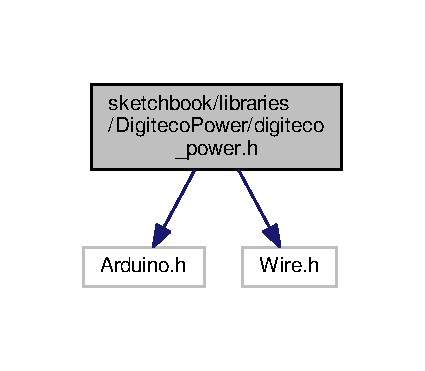
\includegraphics[width=204pt]{digiteco__power_8h__incl}
\end{center}
\end{figure}
This graph shows which files directly or indirectly include this file\+:\nopagebreak
\begin{figure}[H]
\begin{center}
\leavevmode
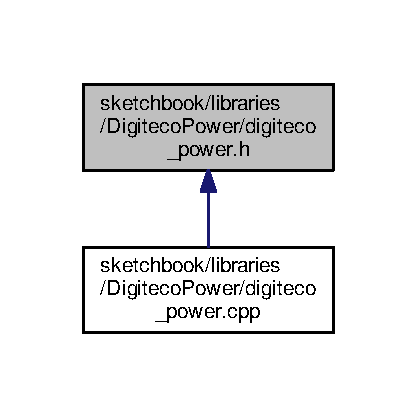
\includegraphics[width=200pt]{digiteco__power_8h__dep__incl}
\end{center}
\end{figure}
\subsection*{Namespaces}
\begin{DoxyCompactItemize}
\item 
 \hyperlink{namespaceDigitecoPower}{Digiteco\+Power}
\begin{DoxyCompactList}\small\item\em \hyperlink{namespaceDigitecoPower}{Digiteco\+Power} namespace. \end{DoxyCompactList}\end{DoxyCompactItemize}
\subsection*{Macros}
\begin{DoxyCompactItemize}
\item 
\mbox{\Hypertarget{digiteco__power_8h_aa8deb23e82d0f30f684e2cecbfc8b146}\label{digiteco__power_8h_aa8deb23e82d0f30f684e2cecbfc8b146}} 
\#define \hyperlink{digiteco__power_8h_aa8deb23e82d0f30f684e2cecbfc8b146}{D\+I\+G\+I\+T\+E\+C\+O\+\_\+\+P\+O\+W\+E\+R\+\_\+\+D\+E\+F\+A\+U\+L\+T\+\_\+\+A\+D\+D\+R\+E\+SS}~(0x30)
\begin{DoxyCompactList}\small\item\em I2C address. \end{DoxyCompactList}\item 
\mbox{\Hypertarget{digiteco__power_8h_a2f55faaba5cd777a035ef225338b7497}\label{digiteco__power_8h_a2f55faaba5cd777a035ef225338b7497}} 
\#define \hyperlink{digiteco__power_8h_a2f55faaba5cd777a035ef225338b7497}{D\+I\+G\+I\+T\+E\+C\+O\+\_\+\+P\+O\+W\+E\+R\+\_\+\+R\+E\+A\+D\+\_\+\+D\+A\+T\+A\+\_\+\+L\+E\+N\+G\+TH}~(4)
\begin{DoxyCompactList}\small\item\em Read data length in numbers of bytes. \end{DoxyCompactList}\item 
\mbox{\Hypertarget{digiteco__power_8h_a253fda21968e718264608f907bbeac5b}\label{digiteco__power_8h_a253fda21968e718264608f907bbeac5b}} 
\#define \hyperlink{digiteco__power_8h_a253fda21968e718264608f907bbeac5b}{D\+I\+G\+I\+T\+E\+C\+O\+\_\+\+P\+O\+W\+E\+R\+\_\+\+I\+N\+P\+U\+T\+\_\+\+V\+O\+L\+T\+A\+G\+E\+\_\+\+A\+D\+D\+R\+E\+SS}~(0)
\begin{DoxyCompactList}\small\item\em I2C input voltage read address. \end{DoxyCompactList}\item 
\mbox{\Hypertarget{digiteco__power_8h_ad018f5da715615cd840a6cf765d2d5bf}\label{digiteco__power_8h_ad018f5da715615cd840a6cf765d2d5bf}} 
\#define \hyperlink{digiteco__power_8h_ad018f5da715615cd840a6cf765d2d5bf}{D\+I\+G\+I\+T\+E\+C\+O\+\_\+\+P\+O\+W\+E\+R\+\_\+\+I\+N\+P\+U\+T\+\_\+\+C\+U\+R\+R\+E\+N\+T\+\_\+\+A\+D\+D\+R\+E\+SS}~(1)
\begin{DoxyCompactList}\small\item\em I2C input current read address. \end{DoxyCompactList}\item 
\mbox{\Hypertarget{digiteco__power_8h_a7094a7cbca7a206e7f9b590ef002d501}\label{digiteco__power_8h_a7094a7cbca7a206e7f9b590ef002d501}} 
\#define \hyperlink{digiteco__power_8h_a7094a7cbca7a206e7f9b590ef002d501}{D\+I\+G\+I\+T\+E\+C\+O\+\_\+\+P\+O\+W\+E\+R\+\_\+\+B\+A\+T\+T\+E\+R\+Y\+\_\+\+V\+O\+L\+T\+A\+G\+E\+\_\+\+A\+D\+D\+R\+E\+SS}~(2)
\begin{DoxyCompactList}\small\item\em I2C input battery voltage read address. \end{DoxyCompactList}\item 
\mbox{\Hypertarget{digiteco__power_8h_a1c83becacdace25fd429d805f9db0cc6}\label{digiteco__power_8h_a1c83becacdace25fd429d805f9db0cc6}} 
\#define \hyperlink{digiteco__power_8h_a1c83becacdace25fd429d805f9db0cc6}{D\+I\+G\+I\+T\+E\+C\+O\+\_\+\+P\+O\+W\+E\+R\+\_\+\+B\+A\+T\+T\+E\+R\+Y\+\_\+\+C\+U\+R\+R\+E\+N\+T\+\_\+\+A\+D\+D\+R\+E\+SS}~(3)
\begin{DoxyCompactList}\small\item\em I2C input battery current read address. \end{DoxyCompactList}\item 
\mbox{\Hypertarget{digiteco__power_8h_a094fe61fa8191acc80dde2d138df28c7}\label{digiteco__power_8h_a094fe61fa8191acc80dde2d138df28c7}} 
\#define \hyperlink{digiteco__power_8h_a094fe61fa8191acc80dde2d138df28c7}{D\+I\+G\+I\+T\+E\+C\+O\+\_\+\+P\+O\+W\+E\+R\+\_\+\+B\+A\+T\+T\+E\+R\+Y\+\_\+\+C\+H\+A\+R\+G\+E\+\_\+\+A\+D\+D\+R\+E\+SS}~(4)
\begin{DoxyCompactList}\small\item\em I2C input battery charge percentage read address. \end{DoxyCompactList}\item 
\mbox{\Hypertarget{digiteco__power_8h_a5a99a63cee1474307f90a3ab572c4eb3}\label{digiteco__power_8h_a5a99a63cee1474307f90a3ab572c4eb3}} 
\#define \hyperlink{digiteco__power_8h_a5a99a63cee1474307f90a3ab572c4eb3}{D\+I\+G\+I\+T\+E\+C\+O\+\_\+\+P\+O\+W\+E\+R\+\_\+\+O\+U\+T\+P\+U\+T\+\_\+\+V\+O\+L\+T\+A\+G\+E\+\_\+\+A\+D\+D\+R\+E\+SS}~(5)
\begin{DoxyCompactList}\small\item\em I2C output voltage read address. \end{DoxyCompactList}\end{DoxyCompactItemize}
\subsection*{Functions}
\begin{DoxyCompactItemize}
\item 
bool \hyperlink{namespaceDigitecoPower_adb7461d6d597526eace685d0365732b7}{Digiteco\+Power\+::de\+\_\+read} (uint8\+\_\+t address, float $\ast$value)
\begin{DoxyCompactList}\small\item\em Read value at specified i2c-\/address. \end{DoxyCompactList}\item 
bool \hyperlink{namespaceDigitecoPower_a2a1d64ce6df863e91fef034a496220fd}{Digiteco\+Power\+::de\+\_\+send} (uint8\+\_\+t address, uint8\+\_\+t data)
\begin{DoxyCompactList}\small\item\em Send data at specified i2c-\/address. \end{DoxyCompactList}\end{DoxyCompactItemize}

\hypertarget{hyt2x1_8cpp}{}\section{sketchbook/libraries/\+H\+Y\+T2\+X1/hyt2x1.cpp File Reference}
\label{hyt2x1_8cpp}\index{sketchbook/libraries/\+H\+Y\+T2\+X1/hyt2x1.\+cpp@{sketchbook/libraries/\+H\+Y\+T2\+X1/hyt2x1.\+cpp}}
{\ttfamily \#include \char`\"{}hyt2x1.\+h\char`\"{}}\newline
Include dependency graph for hyt2x1.\+cpp\+:\nopagebreak
\begin{figure}[H]
\begin{center}
\leavevmode
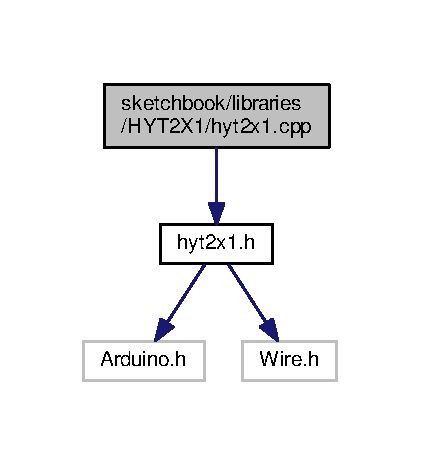
\includegraphics[width=202pt]{hyt2x1_8cpp__incl}
\end{center}
\end{figure}
\subsection*{Namespaces}
\begin{DoxyCompactItemize}
\item 
 \hyperlink{namespaceHyt2X1}{Hyt2\+X1}
\begin{DoxyCompactList}\small\item\em H\+Y\+T2\+X1 namespace. \end{DoxyCompactList}\end{DoxyCompactItemize}
\subsection*{Functions}
\begin{DoxyCompactItemize}
\item 
uint32\+\_\+t \hyperlink{namespaceHyt2X1_a240a988351da007adac832e7ffb851c9}{Hyt2\+X1\+::hyt\+\_\+init\+Read} (uint8\+\_\+t address)
\begin{DoxyCompactList}\small\item\em Init sensor read. \end{DoxyCompactList}\item 
bool \hyperlink{namespaceHyt2X1_a69220922c024c6ab149fee8ad4080a5d}{Hyt2\+X1\+::hyt\+\_\+read} (int8\+\_\+t address, float $\ast$humidity, float $\ast$temperature)
\begin{DoxyCompactList}\small\item\em Returns the humidty and temperature from hyt2\+X1 sensor at specified address. \end{DoxyCompactList}\item 
void \hyperlink{namespaceHyt2X1_a968bbf2c9acb17b73e0d7d5ac12bf575}{Hyt2\+X1\+::hyt\+\_\+send} (int8\+\_\+t address, uint8\+\_\+t data\+\_\+0, uint8\+\_\+t data\+\_\+1, uint8\+\_\+t data\+\_\+2)
\begin{DoxyCompactList}\small\item\em Send sensor command. \end{DoxyCompactList}\item 
void \hyperlink{namespaceHyt2X1_a50b36c601c9bddb5c26ca1b0b9d36458}{Hyt2\+X1\+::hyt\+\_\+change\+Address} (uint8\+\_\+t power\+\_\+pin, int8\+\_\+t address, int8\+\_\+t new\+\_\+address)
\begin{DoxyCompactList}\small\item\em Change sensor address. \end{DoxyCompactList}\item 
void \hyperlink{namespaceHyt2X1_ae551ea888fff17a685ded74f1ef12635}{Hyt2\+X1\+::hyt\+\_\+init} (uint8\+\_\+t power\+\_\+pin)
\begin{DoxyCompactList}\small\item\em Init sensor. \end{DoxyCompactList}\item 
void \hyperlink{namespaceHyt2X1_a54218ca8823fdbd3128f658abe6e1e52}{Hyt2\+X1\+::hyt\+\_\+on} (uint8\+\_\+t power\+\_\+pin)
\begin{DoxyCompactList}\small\item\em Power on sensor. \end{DoxyCompactList}\item 
void \hyperlink{namespaceHyt2X1_a950d46e4e993f893d99139d0443d7ca3}{Hyt2\+X1\+::hyt\+\_\+off} (uint8\+\_\+t power\+\_\+pin)
\begin{DoxyCompactList}\small\item\em Power off sensor. \end{DoxyCompactList}\end{DoxyCompactItemize}

\hypertarget{hyt2x1_8h}{}\section{sketchbook/libraries/\+H\+Y\+T2\+X1/hyt2x1.h File Reference}
\label{hyt2x1_8h}\index{sketchbook/libraries/\+H\+Y\+T2\+X1/hyt2x1.\+h@{sketchbook/libraries/\+H\+Y\+T2\+X1/hyt2x1.\+h}}
{\ttfamily \#include \char`\"{}Arduino.\+h\char`\"{}}\newline
{\ttfamily \#include $<$Wire.\+h$>$}\newline
Include dependency graph for hyt2x1.\+h\+:\nopagebreak
\begin{figure}[H]
\begin{center}
\leavevmode
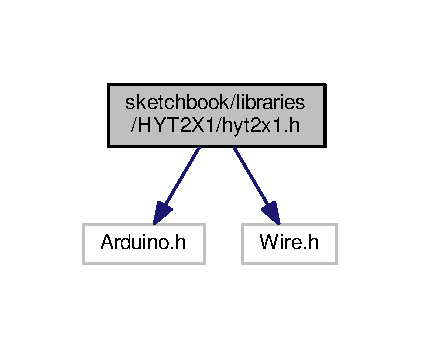
\includegraphics[width=202pt]{hyt2x1_8h__incl}
\end{center}
\end{figure}
This graph shows which files directly or indirectly include this file\+:\nopagebreak
\begin{figure}[H]
\begin{center}
\leavevmode
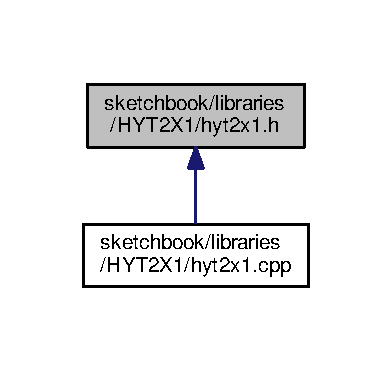
\includegraphics[width=188pt]{hyt2x1_8h__dep__incl}
\end{center}
\end{figure}
\subsection*{Namespaces}
\begin{DoxyCompactItemize}
\item 
 \hyperlink{namespaceHyt2X1}{Hyt2\+X1}
\begin{DoxyCompactList}\small\item\em H\+Y\+T2\+X1 namespace. \end{DoxyCompactList}\end{DoxyCompactItemize}
\subsection*{Macros}
\begin{DoxyCompactItemize}
\item 
\mbox{\Hypertarget{hyt2x1_8h_a120f62242e71b34fb01ca1904fd13112}\label{hyt2x1_8h_a120f62242e71b34fb01ca1904fd13112}} 
\#define \hyperlink{hyt2x1_8h_a120f62242e71b34fb01ca1904fd13112}{H\+Y\+T2\+X1\+\_\+\+D\+E\+F\+A\+U\+L\+T\+\_\+\+A\+D\+D\+R\+E\+SS}~(0x28)
\begin{DoxyCompactList}\small\item\em Default address. \end{DoxyCompactList}\item 
\mbox{\Hypertarget{hyt2x1_8h_a9603babe84e5c9e5ef910a52fca9194f}\label{hyt2x1_8h_a9603babe84e5c9e5ef910a52fca9194f}} 
\#define \hyperlink{hyt2x1_8h_a9603babe84e5c9e5ef910a52fca9194f}{H\+Y\+T2\+X1\+\_\+\+R\+E\+A\+D\+\_\+\+H\+T\+\_\+\+D\+A\+T\+A\+\_\+\+L\+E\+N\+G\+TH}~(4)
\begin{DoxyCompactList}\small\item\em Number of bytes to be read. \end{DoxyCompactList}\item 
\mbox{\Hypertarget{hyt2x1_8h_a20351d7b7f39273a64819751d617e3da}\label{hyt2x1_8h_a20351d7b7f39273a64819751d617e3da}} 
\#define \hyperlink{hyt2x1_8h_a20351d7b7f39273a64819751d617e3da}{H\+Y\+T2\+X1\+\_\+\+E\+N\+T\+E\+R\+\_\+\+C\+O\+M\+M\+A\+N\+D\+\_\+\+M\+O\+DE}~(0x\+A0)
\begin{DoxyCompactList}\small\item\em Command mode. \end{DoxyCompactList}\item 
\mbox{\Hypertarget{hyt2x1_8h_abf498c5fba7c5a501a36698cac1f131b}\label{hyt2x1_8h_abf498c5fba7c5a501a36698cac1f131b}} 
\#define \hyperlink{hyt2x1_8h_abf498c5fba7c5a501a36698cac1f131b}{H\+Y\+T2\+X1\+\_\+\+E\+X\+I\+T\+\_\+\+C\+O\+M\+M\+A\+N\+D\+\_\+\+M\+O\+DE}~(0x80)
\begin{DoxyCompactList}\small\item\em Exit command mode. \end{DoxyCompactList}\item 
\mbox{\Hypertarget{hyt2x1_8h_a836a95d023481badcc84a5f31d9f95a6}\label{hyt2x1_8h_a836a95d023481badcc84a5f31d9f95a6}} 
\#define \hyperlink{hyt2x1_8h_a836a95d023481badcc84a5f31d9f95a6}{H\+Y\+T2\+X1\+\_\+\+W\+R\+I\+T\+E\+\_\+\+A\+D\+D\+R\+E\+SS}~(0x5\+C)
\begin{DoxyCompactList}\small\item\em Write address. \end{DoxyCompactList}\item 
\mbox{\Hypertarget{hyt2x1_8h_ad4162be756170c512c20dea6ccf32a17}\label{hyt2x1_8h_ad4162be756170c512c20dea6ccf32a17}} 
\#define \hyperlink{hyt2x1_8h_ad4162be756170c512c20dea6ccf32a17}{H\+Y\+T2\+X1\+\_\+\+C\+O\+N\+V\+E\+R\+S\+I\+O\+N\+\_\+\+T\+I\+M\+E\+\_\+\+MS}~(100)
\begin{DoxyCompactList}\small\item\em Conversion time in milliseconds. \end{DoxyCompactList}\item 
\mbox{\Hypertarget{hyt2x1_8h_adfc562673f05e37558390033dcb0abc3}\label{hyt2x1_8h_adfc562673f05e37558390033dcb0abc3}} 
\#define \hyperlink{hyt2x1_8h_adfc562673f05e37558390033dcb0abc3}{H\+Y\+T2\+X1\+\_\+\+T\+E\+M\+P\+E\+R\+A\+T\+U\+R\+E\+\_\+\+M\+IN}~(-\/40)
\begin{DoxyCompactList}\small\item\em Minimum temperature. \end{DoxyCompactList}\item 
\mbox{\Hypertarget{hyt2x1_8h_a08f1e6f8f3b56531cfb988ac5e2e4140}\label{hyt2x1_8h_a08f1e6f8f3b56531cfb988ac5e2e4140}} 
\#define \hyperlink{hyt2x1_8h_a08f1e6f8f3b56531cfb988ac5e2e4140}{H\+Y\+T2\+X1\+\_\+\+T\+E\+M\+P\+E\+R\+A\+T\+U\+R\+E\+\_\+\+M\+AX}~(125)
\begin{DoxyCompactList}\small\item\em Maximum temperature. \end{DoxyCompactList}\item 
\mbox{\Hypertarget{hyt2x1_8h_ad131c698960ea1dce05662be6da41a98}\label{hyt2x1_8h_ad131c698960ea1dce05662be6da41a98}} 
\#define \hyperlink{hyt2x1_8h_ad131c698960ea1dce05662be6da41a98}{H\+Y\+T2\+X1\+\_\+\+H\+U\+M\+I\+D\+I\+T\+Y\+\_\+\+M\+IN}~(0)
\begin{DoxyCompactList}\small\item\em Minimum humidity. \end{DoxyCompactList}\item 
\mbox{\Hypertarget{hyt2x1_8h_a662d874ec5045ecb6605319f9ed47d5a}\label{hyt2x1_8h_a662d874ec5045ecb6605319f9ed47d5a}} 
\#define \hyperlink{hyt2x1_8h_a662d874ec5045ecb6605319f9ed47d5a}{H\+Y\+T2\+X1\+\_\+\+H\+U\+M\+I\+D\+I\+T\+Y\+\_\+\+M\+AX}~(100)
\begin{DoxyCompactList}\small\item\em Maximum humidity. \end{DoxyCompactList}\end{DoxyCompactItemize}
\subsection*{Functions}
\begin{DoxyCompactItemize}
\item 
void \hyperlink{namespaceHyt2X1_ae551ea888fff17a685ded74f1ef12635}{Hyt2\+X1\+::hyt\+\_\+init} (uint8\+\_\+t power\+\_\+pin)
\begin{DoxyCompactList}\small\item\em Init sensor. \end{DoxyCompactList}\item 
void \hyperlink{namespaceHyt2X1_a54218ca8823fdbd3128f658abe6e1e52}{Hyt2\+X1\+::hyt\+\_\+on} (uint8\+\_\+t power\+\_\+pin)
\begin{DoxyCompactList}\small\item\em Power on sensor. \end{DoxyCompactList}\item 
void \hyperlink{namespaceHyt2X1_a950d46e4e993f893d99139d0443d7ca3}{Hyt2\+X1\+::hyt\+\_\+off} (uint8\+\_\+t power\+\_\+pin)
\begin{DoxyCompactList}\small\item\em Power off sensor. \end{DoxyCompactList}\item 
void \hyperlink{namespaceHyt2X1_a50b36c601c9bddb5c26ca1b0b9d36458}{Hyt2\+X1\+::hyt\+\_\+change\+Address} (uint8\+\_\+t power\+\_\+pin, int8\+\_\+t address, int8\+\_\+t new\+\_\+address)
\begin{DoxyCompactList}\small\item\em Change sensor address. \end{DoxyCompactList}\item 
uint32\+\_\+t \hyperlink{namespaceHyt2X1_a240a988351da007adac832e7ffb851c9}{Hyt2\+X1\+::hyt\+\_\+init\+Read} (uint8\+\_\+t address)
\begin{DoxyCompactList}\small\item\em Init sensor read. \end{DoxyCompactList}\item 
bool \hyperlink{namespaceHyt2X1_a69220922c024c6ab149fee8ad4080a5d}{Hyt2\+X1\+::hyt\+\_\+read} (int8\+\_\+t address, float $\ast$humidity, float $\ast$temperature)
\begin{DoxyCompactList}\small\item\em Returns the humidty and temperature from hyt2\+X1 sensor at specified address. \end{DoxyCompactList}\item 
void \hyperlink{namespaceHyt2X1_a968bbf2c9acb17b73e0d7d5ac12bf575}{Hyt2\+X1\+::hyt\+\_\+send} (int8\+\_\+t address, uint8\+\_\+t data\+\_\+0, uint8\+\_\+t data\+\_\+1, uint8\+\_\+t data\+\_\+2)
\begin{DoxyCompactList}\small\item\em Send sensor command. \end{DoxyCompactList}\end{DoxyCompactItemize}

\hypertarget{ntp_8cpp}{}\section{sketchbook/libraries/\+N\+T\+P/ntp.cpp File Reference}
\label{ntp_8cpp}\index{sketchbook/libraries/\+N\+T\+P/ntp.\+cpp@{sketchbook/libraries/\+N\+T\+P/ntp.\+cpp}}
{\ttfamily \#include \char`\"{}ntp.\+h\char`\"{}}\newline
Include dependency graph for ntp.\+cpp\+:\nopagebreak
\begin{figure}[H]
\begin{center}
\leavevmode
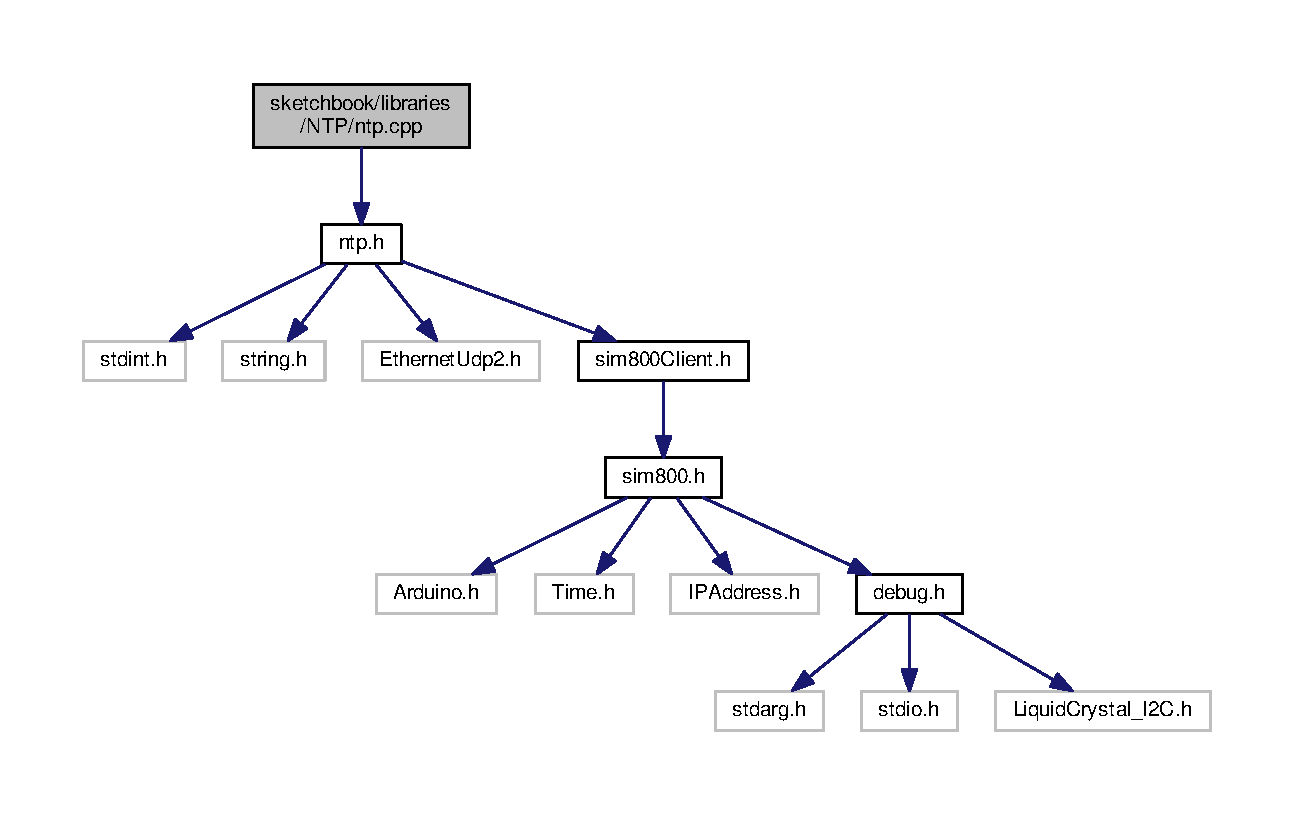
\includegraphics[width=350pt]{ntp_8cpp__incl}
\end{center}
\end{figure}

\hypertarget{ntp_8h}{}\section{sketchbook/libraries/\+N\+T\+P/ntp.h File Reference}
\label{ntp_8h}\index{sketchbook/libraries/\+N\+T\+P/ntp.\+h@{sketchbook/libraries/\+N\+T\+P/ntp.\+h}}
{\ttfamily \#include $<$stdint.\+h$>$}\newline
{\ttfamily \#include $<$string.\+h$>$}\newline
{\ttfamily \#include $<$Ethernet\+Udp2.\+h$>$}\newline
{\ttfamily \#include $<$sim800\+Client.\+h$>$}\newline
Include dependency graph for ntp.\+h\+:\nopagebreak
\begin{figure}[H]
\begin{center}
\leavevmode
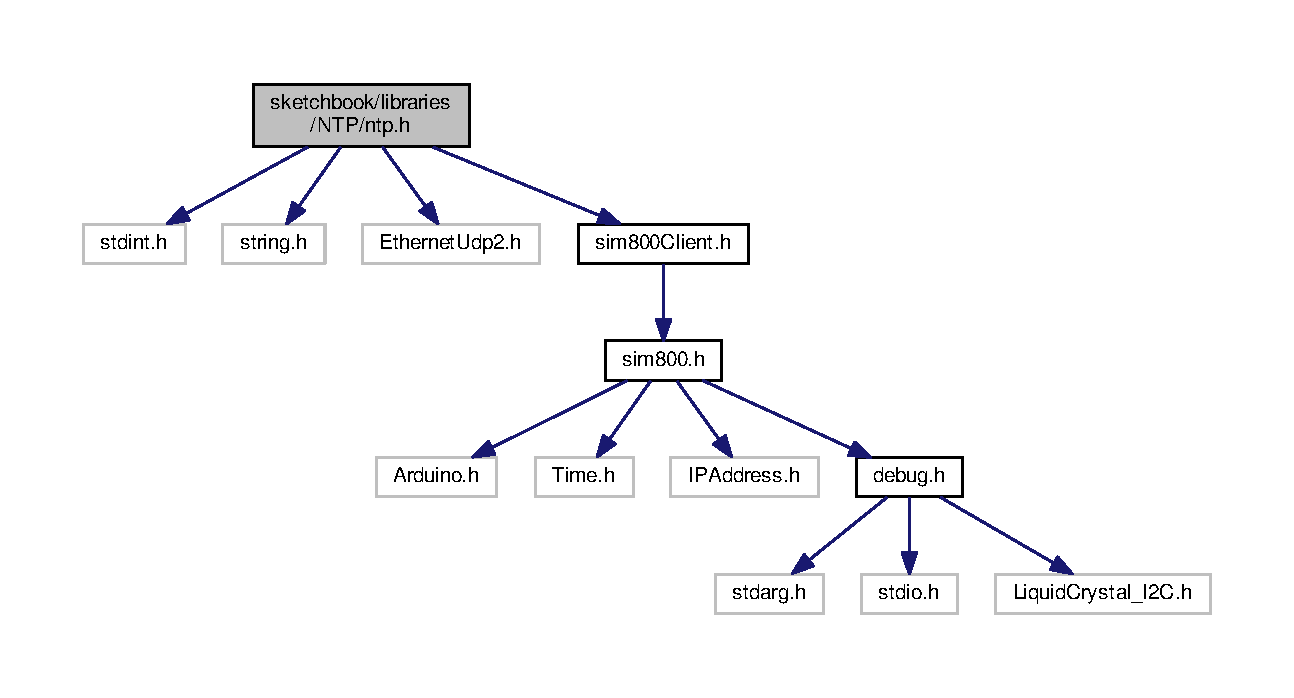
\includegraphics[width=350pt]{ntp_8h__incl}
\end{center}
\end{figure}
This graph shows which files directly or indirectly include this file\+:\nopagebreak
\begin{figure}[H]
\begin{center}
\leavevmode
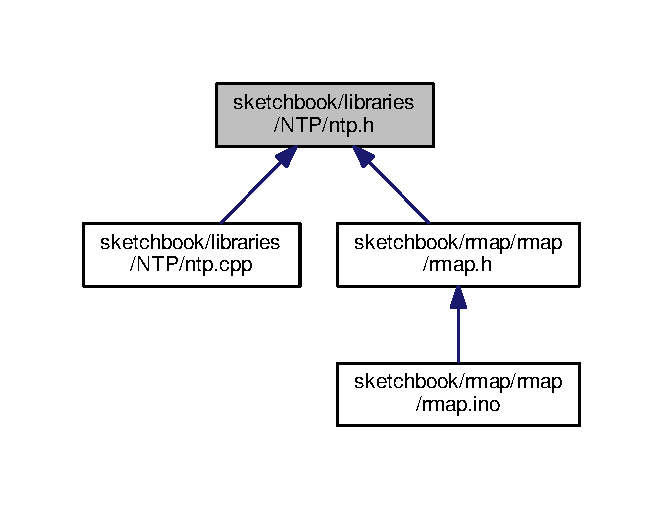
\includegraphics[width=184pt]{ntp_8h__dep__incl}
\end{center}
\end{figure}
\subsection*{Classes}
\begin{DoxyCompactItemize}
\item 
class \hyperlink{classNtp}{Ntp}
\begin{DoxyCompactList}\small\item\em \hyperlink{classNtp}{Ntp} class. \end{DoxyCompactList}\end{DoxyCompactItemize}
\subsection*{Macros}
\begin{DoxyCompactItemize}
\item 
\mbox{\Hypertarget{ntp_8h_a57df452a6d54697643631ce3039623d4}\label{ntp_8h_a57df452a6d54697643631ce3039623d4}} 
\#define \hyperlink{ntp_8h_a57df452a6d54697643631ce3039623d4}{N\+T\+P\+\_\+\+S\+E\+R\+V\+E\+R\+\_\+\+P\+O\+RT}~(123)
\begin{DoxyCompactList}\small\item\em N\+TP server port. \end{DoxyCompactList}\item 
\mbox{\Hypertarget{ntp_8h_aa1c0658c928d132f60e25b16771be754}\label{ntp_8h_aa1c0658c928d132f60e25b16771be754}} 
\#define \hyperlink{ntp_8h_aa1c0658c928d132f60e25b16771be754}{N\+T\+P\+\_\+\+P\+A\+C\+K\+E\+T\+\_\+\+L\+E\+N\+G\+TH}~(48)
\begin{DoxyCompactList}\small\item\em N\+TP packet length. \end{DoxyCompactList}\item 
\mbox{\Hypertarget{ntp_8h_ace39986119607151c9b16cecf698abe1}\label{ntp_8h_ace39986119607151c9b16cecf698abe1}} 
\#define \hyperlink{ntp_8h_ace39986119607151c9b16cecf698abe1}{N\+T\+P\+\_\+\+R\+E\+C\+E\+I\+V\+E\+\_\+\+T\+I\+M\+E\+S\+T\+A\+M\+P\+\_\+\+O\+F\+F\+S\+ET}~(40)
\begin{DoxyCompactList}\small\item\em N\+TP received timestamp offset. \end{DoxyCompactList}\item 
\mbox{\Hypertarget{ntp_8h_a7c6347c9dc2a84fc9f90d6eaca9df2ca}\label{ntp_8h_a7c6347c9dc2a84fc9f90d6eaca9df2ca}} 
\#define \hyperlink{ntp_8h_a7c6347c9dc2a84fc9f90d6eaca9df2ca}{N\+T\+P\+\_\+1\+\_\+\+H\+O\+U\+R\+\_\+\+S\+E\+C\+O\+N\+DS}~(3600\+U\+L)
\begin{DoxyCompactList}\small\item\em seconds in one hour. \end{DoxyCompactList}\item 
\mbox{\Hypertarget{ntp_8h_a2805f547f7dc24f8477827a4120d7385}\label{ntp_8h_a2805f547f7dc24f8477827a4120d7385}} 
\#define \hyperlink{ntp_8h_a2805f547f7dc24f8477827a4120d7385}{N\+T\+P\+\_\+70\+\_\+\+Y\+E\+A\+R\+S\+\_\+\+S\+E\+C\+O\+N\+DS}~(2208988800\+U\+L)
\begin{DoxyCompactList}\small\item\em seconds in 70 years. \end{DoxyCompactList}\item 
\mbox{\Hypertarget{ntp_8h_a004ce391c29e30cea2c3f958adfd009e}\label{ntp_8h_a004ce391c29e30cea2c3f958adfd009e}} 
\#define \hyperlink{ntp_8h_a004ce391c29e30cea2c3f958adfd009e}{N\+T\+P\+\_\+\+V\+A\+L\+I\+D\+\_\+\+S\+T\+A\+R\+T\+\_\+\+T\+I\+M\+E\+\_\+S}~(1483228800\+U\+L)
\begin{DoxyCompactList}\small\item\em seconds for 00\+:00\+:00 01/01/2017 since 00\+:00\+:00 01/01/1970. \end{DoxyCompactList}\item 
\mbox{\Hypertarget{ntp_8h_a812dbabea90c19f0a440aeeb8d20fce3}\label{ntp_8h_a812dbabea90c19f0a440aeeb8d20fce3}} 
\#define \hyperlink{ntp_8h_a812dbabea90c19f0a440aeeb8d20fce3}{N\+T\+P\+\_\+\+T\+I\+M\+E\+Z\+O\+NE}~(0)
\begin{DoxyCompactList}\small\item\em N\+TP timezone is set to G\+MT. \end{DoxyCompactList}\end{DoxyCompactItemize}

\hypertarget{pcf8563_8cpp}{}\section{sketchbook/libraries/\+P\+C\+F8563/pcf8563.cpp File Reference}
\label{pcf8563_8cpp}\index{sketchbook/libraries/\+P\+C\+F8563/pcf8563.\+cpp@{sketchbook/libraries/\+P\+C\+F8563/pcf8563.\+cpp}}
{\ttfamily \#include \char`\"{}pcf8563.\+h\char`\"{}}\newline
Include dependency graph for pcf8563.\+cpp\+:\nopagebreak
\begin{figure}[H]
\begin{center}
\leavevmode
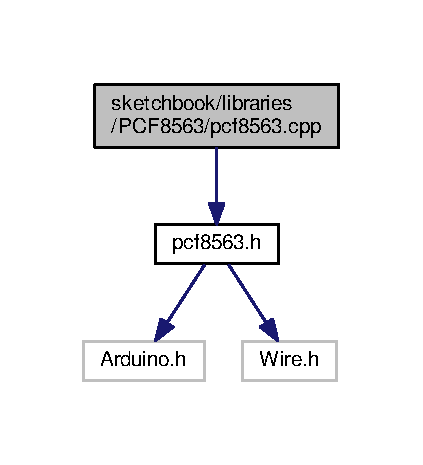
\includegraphics[width=203pt]{pcf8563_8cpp__incl}
\end{center}
\end{figure}
\subsection*{Namespaces}
\begin{DoxyCompactItemize}
\item 
 \hyperlink{namespacePcf8563}{Pcf8563}
\begin{DoxyCompactList}\small\item\em \hyperlink{namespacePcf8563}{Pcf8563} namespace. \end{DoxyCompactList}\end{DoxyCompactItemize}
\subsection*{Functions}
\begin{DoxyCompactItemize}
\item 
uint8\+\_\+t \hyperlink{namespacePcf8563_aae506e83df33a718bdd0dd184d42c19a}{Pcf8563\+::bcd\+To\+Dec} (uint8\+\_\+t val)
\begin{DoxyCompactList}\small\item\em Convert a value from B\+CD format into decimal format. \end{DoxyCompactList}\item 
uint8\+\_\+t \hyperlink{namespacePcf8563_a3519616ff3c2de84e2ea54442ef0ed0c}{Pcf8563\+::dec\+To\+Bcd} (uint8\+\_\+t val)
\begin{DoxyCompactList}\small\item\em Convert a value from decimal format into B\+CD format. \end{DoxyCompactList}\item 
bool \hyperlink{namespacePcf8563_abe54082b4f23e40ef4f5be845b5cf008}{Pcf8563\+::reset} ()
\begin{DoxyCompactList}\small\item\em Reset P\+C\+F8563. \end{DoxyCompactList}\item 
bool \hyperlink{namespacePcf8563_a32420d263d406b766b21bc00dccdc333}{Pcf8563\+::enable} ()
\begin{DoxyCompactList}\small\item\em Enable P\+C\+F8563 counter. \end{DoxyCompactList}\item 
bool \hyperlink{namespacePcf8563_a1920171d3aec259327a124b712299a04}{Pcf8563\+::disable} ()
\begin{DoxyCompactList}\small\item\em Disable P\+C\+F8563 counter. \end{DoxyCompactList}\item 
bool \hyperlink{namespacePcf8563_a098f161f3396c8ed0c2f11c7193f5b0d}{Pcf8563\+::get\+Control\+Status1} (uint8\+\_\+t $\ast$control\+\_\+status\+\_\+1)
\begin{DoxyCompactList}\small\item\em Read control status 1 register. \end{DoxyCompactList}\item 
bool \hyperlink{namespacePcf8563_a17680b8e68d064bb39007b4a6afc240e}{Pcf8563\+::set\+Control\+Status1} (uint8\+\_\+t control\+\_\+status\+\_\+1)
\begin{DoxyCompactList}\small\item\em Write control status 1 register. \end{DoxyCompactList}\item 
bool \hyperlink{namespacePcf8563_a6cf47400c4e974b9d9a1bf1d1a9e463d}{Pcf8563\+::get\+Control\+Status2} (uint8\+\_\+t $\ast$control\+\_\+status\+\_\+2)
\begin{DoxyCompactList}\small\item\em Read control status 2 register. \end{DoxyCompactList}\item 
bool \hyperlink{namespacePcf8563_ac23ff9ec298a4ec5a777139d972b5e4b}{Pcf8563\+::set\+Control\+Status2} (uint8\+\_\+t control\+\_\+status\+\_\+2)
\begin{DoxyCompactList}\small\item\em Write control status 2 register. \end{DoxyCompactList}\item 
bool \hyperlink{namespacePcf8563_aa6afef0bd9005fc8b8332c7cb82ec6ce}{Pcf8563\+::get\+Clockout\+Control} (uint8\+\_\+t $\ast$clockout\+\_\+control)
\begin{DoxyCompactList}\small\item\em Read clockout control register. \end{DoxyCompactList}\item 
bool \hyperlink{namespacePcf8563_a52b2a6f5b28f961e7e4bece212c7bdd6}{Pcf8563\+::set\+Clockout\+Control} (uint8\+\_\+t clockout\+\_\+control)
\begin{DoxyCompactList}\small\item\em Write clockout control register. \end{DoxyCompactList}\item 
bool \hyperlink{namespacePcf8563_a0aad62263917a9ceec3c12c88a29b835}{Pcf8563\+::get\+Timer\+Control} (uint8\+\_\+t $\ast$timer\+\_\+control)
\begin{DoxyCompactList}\small\item\em Read timer control register. \end{DoxyCompactList}\item 
bool \hyperlink{namespacePcf8563_a112b6debc61100cd3ab737af9d31e119}{Pcf8563\+::set\+Timer\+Control} (uint8\+\_\+t timer\+\_\+control)
\begin{DoxyCompactList}\small\item\em Write timer control register. \end{DoxyCompactList}\item 
bool \hyperlink{namespacePcf8563_aa852ae63d80f0a9137b3910a3b193d89}{Pcf8563\+::get\+Date} (uint8\+\_\+t $\ast$day, uint8\+\_\+t $\ast$month, uint8\+\_\+t $\ast$year, uint8\+\_\+t $\ast$weekday, uint8\+\_\+t $\ast$century)
\begin{DoxyCompactList}\small\item\em Read date register. \end{DoxyCompactList}\item 
bool \hyperlink{namespacePcf8563_aa8a735e59aae37d9184b17cb84de4f85}{Pcf8563\+::set\+Date} (uint8\+\_\+t day, uint8\+\_\+t month, uint8\+\_\+t year, uint8\+\_\+t weekday, uint8\+\_\+t century)
\begin{DoxyCompactList}\small\item\em Write date register. \end{DoxyCompactList}\item 
bool \hyperlink{namespacePcf8563_aaa1099008bec7e232d47ca6056777c23}{Pcf8563\+::get\+Date\+Time} (uint8\+\_\+t $\ast$hours, uint8\+\_\+t $\ast$minutes, uint8\+\_\+t $\ast$seconds, uint8\+\_\+t $\ast$day, uint8\+\_\+t $\ast$month, uint8\+\_\+t $\ast$year, uint8\+\_\+t $\ast$weekday, uint8\+\_\+t $\ast$century)
\begin{DoxyCompactList}\small\item\em Read date and time register. \end{DoxyCompactList}\item 
bool \hyperlink{namespacePcf8563_aeb90b131ae770b2dcb9b167ea3856ed4}{Pcf8563\+::get\+Time} (uint8\+\_\+t $\ast$hours, uint8\+\_\+t $\ast$minutes, uint8\+\_\+t $\ast$seconds)
\begin{DoxyCompactList}\small\item\em Read time register. \end{DoxyCompactList}\item 
bool \hyperlink{namespacePcf8563_a797213f5e675582765df0b42ab921999}{Pcf8563\+::set\+Time} (uint8\+\_\+t hours, uint8\+\_\+t minutes, uint8\+\_\+t seconds)
\begin{DoxyCompactList}\small\item\em Write time register. \end{DoxyCompactList}\item 
bool \hyperlink{namespacePcf8563_a03e4ea0f00fd48664537788ba491fa60}{Pcf8563\+::enable\+Clockout} ()
\begin{DoxyCompactList}\small\item\em Enable clockout frequency. \end{DoxyCompactList}\item 
bool \hyperlink{namespacePcf8563_a76c81b3e0f59f5e4e80dd8807c199856}{Pcf8563\+::disable\+Clockout} ()
\begin{DoxyCompactList}\small\item\em Disable clockout frequency. \end{DoxyCompactList}\item 
bool \hyperlink{namespacePcf8563_a4bc96bd7ccbd30db659536befb3da1fe}{Pcf8563\+::set\+Clockout\+Frequency} (uint8\+\_\+t frequency)
\begin{DoxyCompactList}\small\item\em Set clockout frequency. \end{DoxyCompactList}\item 
bool \hyperlink{namespacePcf8563_ab8ff6484e7a5636187e0212a98f623bf}{Pcf8563\+::is\+Clockout\+Active} ()
\begin{DoxyCompactList}\small\item\em Check if clockout frequency is enabled. \end{DoxyCompactList}\item 
bool \hyperlink{namespacePcf8563_a6e196fe410c080e4f6e20aadbe279637}{Pcf8563\+::enable\+Alarm} ()
\begin{DoxyCompactList}\small\item\em Enable Alarm interrupt. \end{DoxyCompactList}\item 
bool \hyperlink{namespacePcf8563_ad9dd3fe9bf1ab196090357b717c7207d}{Pcf8563\+::disable\+Alarm} ()
\begin{DoxyCompactList}\small\item\em Disable alarm interrupt. \end{DoxyCompactList}\item 
bool \hyperlink{namespacePcf8563_ae554435cc17a3e49d9d731b97e3fc0be}{Pcf8563\+::reset\+Alarm} ()
\begin{DoxyCompactList}\small\item\em Reset alarm. \end{DoxyCompactList}\item 
bool \hyperlink{namespacePcf8563_a23086671303b630318e82e9bef662b44}{Pcf8563\+::is\+Alarm\+Active} ()
\begin{DoxyCompactList}\small\item\em Check if alarm interrupt is enabled. \end{DoxyCompactList}\item 
bool \hyperlink{namespacePcf8563_a687f6854cf03080456bdd8596c1c60ff}{Pcf8563\+::get\+Alarm} (uint8\+\_\+t $\ast$hours, uint8\+\_\+t $\ast$minutes, uint8\+\_\+t $\ast$day, uint8\+\_\+t $\ast$weekday)
\begin{DoxyCompactList}\small\item\em Read alarm register. \end{DoxyCompactList}\item 
bool \hyperlink{namespacePcf8563_ad82df13e3625c1b975f2cc2e7e356f0e}{Pcf8563\+::set\+Alarm} (uint8\+\_\+t hours, uint8\+\_\+t minutes, uint8\+\_\+t day, uint8\+\_\+t weekday)
\begin{DoxyCompactList}\small\item\em Write alarm register. \end{DoxyCompactList}\item 
bool \hyperlink{namespacePcf8563_af4cc94d1ea73bbff5d44e1b716111cdb}{Pcf8563\+::enable\+Timer} ()
\begin{DoxyCompactList}\small\item\em Enable timer interrupt. \end{DoxyCompactList}\item 
bool \hyperlink{namespacePcf8563_ac2c3ca7f3a13516c6549bfc0f6527c6a}{Pcf8563\+::disable\+Timer} ()
\begin{DoxyCompactList}\small\item\em Disable timer interrupt. \end{DoxyCompactList}\item 
bool \hyperlink{namespacePcf8563_a6fd0509d12fd312b5dbed8506b9315c9}{Pcf8563\+::reset\+Timer} ()
\begin{DoxyCompactList}\small\item\em Reset timer. \end{DoxyCompactList}\item 
bool \hyperlink{namespacePcf8563_aab079fef811171abcba7e80b8595a8d1}{Pcf8563\+::is\+Timer\+Active} ()
\begin{DoxyCompactList}\small\item\em Check if timer is enabled. \end{DoxyCompactList}\item 
bool \hyperlink{namespacePcf8563_a338898a456015e796d48b82738d5a8c4}{Pcf8563\+::set\+Timer} (uint8\+\_\+t frequency, uint8\+\_\+t timer)
\begin{DoxyCompactList}\small\item\em Write timer register. \end{DoxyCompactList}\item 
int16\+\_\+t \hyperlink{namespacePcf8563_a7ffd9819a4946feda4117a90ef176ab9}{Pcf8563\+::get\+Days\+From\+Two\+Date} (int16\+\_\+t d1, int16\+\_\+t m1, int16\+\_\+t y1, int16\+\_\+t d2, int16\+\_\+t m2, int16\+\_\+t y2)
\begin{DoxyCompactList}\small\item\em Calculate numbers of days from two date. \end{DoxyCompactList}\item 
uint32\+\_\+t \hyperlink{namespacePcf8563_a2824a08aaed53b49a8fc1aa77cab629d}{Pcf8563\+::get\+Time} ()
\begin{DoxyCompactList}\small\item\em Read date and time and return they as seconds elapsed from 00\+:00\+:00 01/01/1970. \end{DoxyCompactList}\end{DoxyCompactItemize}

\hypertarget{pcf8563_8h}{}\section{sketchbook/libraries/\+P\+C\+F8563/pcf8563.h File Reference}
\label{pcf8563_8h}\index{sketchbook/libraries/\+P\+C\+F8563/pcf8563.\+h@{sketchbook/libraries/\+P\+C\+F8563/pcf8563.\+h}}
{\ttfamily \#include \char`\"{}Arduino.\+h\char`\"{}}\newline
{\ttfamily \#include $<$Wire.\+h$>$}\newline
Include dependency graph for pcf8563.\+h\+:\nopagebreak
\begin{figure}[H]
\begin{center}
\leavevmode
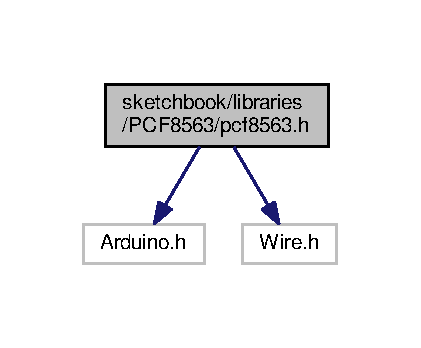
\includegraphics[width=202pt]{pcf8563_8h__incl}
\end{center}
\end{figure}
This graph shows which files directly or indirectly include this file\+:\nopagebreak
\begin{figure}[H]
\begin{center}
\leavevmode
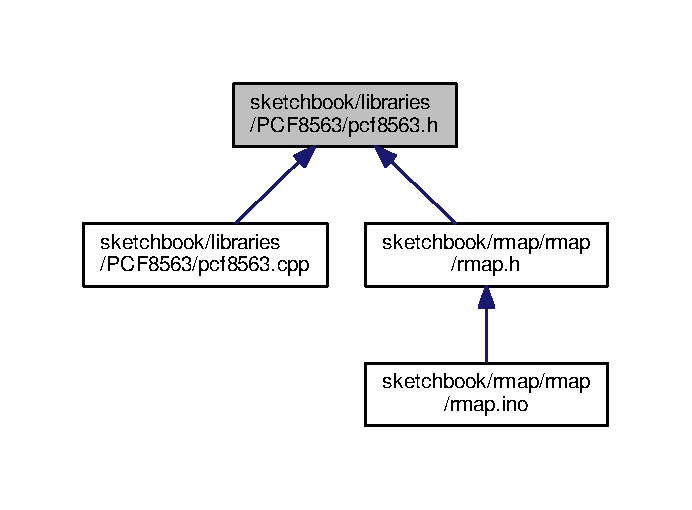
\includegraphics[width=332pt]{pcf8563_8h__dep__incl}
\end{center}
\end{figure}
\subsection*{Namespaces}
\begin{DoxyCompactItemize}
\item 
 \hyperlink{namespacePcf8563}{Pcf8563}
\begin{DoxyCompactList}\small\item\em \hyperlink{namespacePcf8563}{Pcf8563} namespace. \end{DoxyCompactList}\end{DoxyCompactItemize}
\subsection*{Macros}
\begin{DoxyCompactItemize}
\item 
\mbox{\Hypertarget{pcf8563_8h_ad8f013828cbaadce7813a224d980a96c}\label{pcf8563_8h_ad8f013828cbaadce7813a224d980a96c}} 
\#define \hyperlink{pcf8563_8h_ad8f013828cbaadce7813a224d980a96c}{P\+C\+F8563\+\_\+\+R\+E\+A\+D\+\_\+\+A\+D\+D\+R\+E\+SS}~(0x\+A3 $>$$>$ 1)
\begin{DoxyCompactList}\small\item\em I2C read address. \end{DoxyCompactList}\item 
\mbox{\Hypertarget{pcf8563_8h_a21d8ece51034522404eeee69481a0cf8}\label{pcf8563_8h_a21d8ece51034522404eeee69481a0cf8}} 
\#define \hyperlink{pcf8563_8h_a21d8ece51034522404eeee69481a0cf8}{P\+C\+F8563\+\_\+\+W\+R\+I\+T\+E\+\_\+\+A\+D\+D\+R\+E\+SS}~(0x\+A2)
\begin{DoxyCompactList}\small\item\em I2C write address. \end{DoxyCompactList}\item 
\mbox{\Hypertarget{pcf8563_8h_a8c5dcf0f0ff373c1f9d2f22abf542239}\label{pcf8563_8h_a8c5dcf0f0ff373c1f9d2f22abf542239}} 
\#define \hyperlink{pcf8563_8h_a8c5dcf0f0ff373c1f9d2f22abf542239}{P\+C\+F8563\+\_\+\+C\+O\+N\+T\+R\+O\+L\+\_\+\+S\+T\+A\+T\+U\+S\+\_\+1\+\_\+\+A\+D\+D\+R\+E\+SS}~(0x00)
\begin{DoxyCompactList}\small\item\em Control status 1 register i2c address. \end{DoxyCompactList}\item 
\mbox{\Hypertarget{pcf8563_8h_a7bd74aa8863ad00d9307cac803e9dd84}\label{pcf8563_8h_a7bd74aa8863ad00d9307cac803e9dd84}} 
\#define \hyperlink{pcf8563_8h_a7bd74aa8863ad00d9307cac803e9dd84}{P\+C\+F8563\+\_\+\+C\+O\+N\+T\+R\+O\+L\+\_\+\+S\+T\+A\+T\+U\+S\+\_\+2\+\_\+\+A\+D\+D\+R\+E\+SS}~(0x01)
\begin{DoxyCompactList}\small\item\em Control status 2 register i2c address. B\+IT 4\+: T\+I\+\_\+\+TP, B\+IT 3\+: AF, B\+IT 2\+: TF, B\+IT 1\+: A\+IE, B\+IT 0\+: T\+IE. \end{DoxyCompactList}\item 
\mbox{\Hypertarget{pcf8563_8h_a6983e57e032f3df9222f1d4dc166d505}\label{pcf8563_8h_a6983e57e032f3df9222f1d4dc166d505}} 
\#define \hyperlink{pcf8563_8h_a6983e57e032f3df9222f1d4dc166d505}{P\+C\+F8563\+\_\+\+V\+L\+\_\+\+S\+E\+C\+O\+N\+D\+\_\+\+A\+D\+D\+R\+E\+SS}~(0x02)
\begin{DoxyCompactList}\small\item\em VL second register address. B\+IT 0-\/6\+: seconds \mbox{[}0-\/59\mbox{]}, B\+IT 7\+: VL. \end{DoxyCompactList}\item 
\mbox{\Hypertarget{pcf8563_8h_a80c799b490b4eb70b8cbb0a68593c72d}\label{pcf8563_8h_a80c799b490b4eb70b8cbb0a68593c72d}} 
\#define \hyperlink{pcf8563_8h_a80c799b490b4eb70b8cbb0a68593c72d}{P\+C\+F8563\+\_\+\+M\+I\+N\+U\+T\+E\+\_\+\+A\+D\+D\+R\+E\+SS}~(0x03)
\begin{DoxyCompactList}\small\item\em Minute register address. B\+IT 0-\/6\+: minutes \mbox{[}0-\/59\mbox{]}. \end{DoxyCompactList}\item 
\mbox{\Hypertarget{pcf8563_8h_a2eb91f788d87b5260e8ee3ed31a265a4}\label{pcf8563_8h_a2eb91f788d87b5260e8ee3ed31a265a4}} 
\#define \hyperlink{pcf8563_8h_a2eb91f788d87b5260e8ee3ed31a265a4}{P\+C\+F8563\+\_\+\+H\+O\+U\+R\+\_\+\+A\+D\+D\+R\+E\+SS}~(0x04)
\begin{DoxyCompactList}\small\item\em Hour register address. B\+IT 0-\/5\+: hours \mbox{[}0-\/23\mbox{]}. \end{DoxyCompactList}\item 
\mbox{\Hypertarget{pcf8563_8h_af17bb37d629f74400afd9344f63eb779}\label{pcf8563_8h_af17bb37d629f74400afd9344f63eb779}} 
\#define \hyperlink{pcf8563_8h_af17bb37d629f74400afd9344f63eb779}{P\+C\+F8563\+\_\+\+D\+A\+Y\+\_\+\+A\+D\+D\+R\+E\+SS}~(0x05)
\begin{DoxyCompactList}\small\item\em Day register address. B\+IT 0-\/5\+: days \mbox{[}1-\/31\mbox{]}. \end{DoxyCompactList}\item 
\mbox{\Hypertarget{pcf8563_8h_aa9b04f0b276feb2078be5f9ab8f94218}\label{pcf8563_8h_aa9b04f0b276feb2078be5f9ab8f94218}} 
\#define \hyperlink{pcf8563_8h_aa9b04f0b276feb2078be5f9ab8f94218}{P\+C\+F8563\+\_\+\+W\+E\+E\+K\+D\+A\+Y\+\_\+\+A\+D\+D\+R\+E\+SS}~(0x06)
\begin{DoxyCompactList}\small\item\em Weekday register address. B\+IT 0-\/2\+: weekdays \mbox{[}0-\/6\mbox{]} start from Sunday. \end{DoxyCompactList}\item 
\mbox{\Hypertarget{pcf8563_8h_adcfc41a947d952dc512f424eecdd7fe1}\label{pcf8563_8h_adcfc41a947d952dc512f424eecdd7fe1}} 
\#define \hyperlink{pcf8563_8h_adcfc41a947d952dc512f424eecdd7fe1}{P\+C\+F8563\+\_\+\+C\+E\+N\+T\+U\+R\+Y\+\_\+\+M\+O\+N\+T\+H\+S\+\_\+\+A\+D\+D\+R\+E\+SS}~(0x07)
\begin{DoxyCompactList}\small\item\em Century months register address. B\+IT 0-\/4\+: months \mbox{[}1-\/12\mbox{]}, B\+IT 7\+: century \mbox{[}0-\/1\mbox{]}. \end{DoxyCompactList}\item 
\mbox{\Hypertarget{pcf8563_8h_ae2a7adebd4abf8fd076b89c62d7fb835}\label{pcf8563_8h_ae2a7adebd4abf8fd076b89c62d7fb835}} 
\#define \hyperlink{pcf8563_8h_ae2a7adebd4abf8fd076b89c62d7fb835}{P\+C\+F8563\+\_\+\+Y\+E\+A\+R\+\_\+\+A\+D\+D\+R\+E\+SS}~(0x08)
\begin{DoxyCompactList}\small\item\em Year register address. B\+IT 0-\/7\+: year \mbox{[}0-\/99\mbox{]}. \end{DoxyCompactList}\item 
\mbox{\Hypertarget{pcf8563_8h_ad53d7e8aa13ccc403b69e7641cc61bd0}\label{pcf8563_8h_ad53d7e8aa13ccc403b69e7641cc61bd0}} 
\#define \hyperlink{pcf8563_8h_ad53d7e8aa13ccc403b69e7641cc61bd0}{P\+C\+F8563\+\_\+\+M\+I\+N\+U\+T\+E\+\_\+\+A\+L\+A\+R\+M\+\_\+\+A\+D\+D\+R\+E\+SS}~(0x09)
\begin{DoxyCompactList}\small\item\em Minute alarm register address. B\+IT 0-\/6\+: minutes alarm \mbox{[}0-\/59\mbox{]}, B\+IT 7\+: A\+E\+\_\+M (0\+: enable, 1\+: disable) \end{DoxyCompactList}\item 
\mbox{\Hypertarget{pcf8563_8h_a9060a94690f7eda74b5fa1bf751dcd85}\label{pcf8563_8h_a9060a94690f7eda74b5fa1bf751dcd85}} 
\#define \hyperlink{pcf8563_8h_a9060a94690f7eda74b5fa1bf751dcd85}{P\+C\+F8563\+\_\+\+H\+O\+U\+R\+\_\+\+A\+L\+A\+R\+M\+\_\+\+A\+D\+D\+R\+E\+SS}~(0x0\+A)
\begin{DoxyCompactList}\small\item\em Hour alarm register address. B\+IT 0-\/5\+: hours alarm \mbox{[}0-\/23\mbox{]}, B\+IT 7\+: A\+E\+\_\+H (0\+: enable, 1\+: disable) \end{DoxyCompactList}\item 
\mbox{\Hypertarget{pcf8563_8h_a44980c2c4b1898b3ff0dee1c036cfd9c}\label{pcf8563_8h_a44980c2c4b1898b3ff0dee1c036cfd9c}} 
\#define \hyperlink{pcf8563_8h_a44980c2c4b1898b3ff0dee1c036cfd9c}{P\+C\+F8563\+\_\+\+D\+A\+Y\+\_\+\+A\+L\+A\+R\+M\+\_\+\+A\+D\+D\+R\+E\+SS}~(0x0\+B)
\begin{DoxyCompactList}\small\item\em Day alarm register address. B\+IT 0-\/5\+: days alarm \mbox{[}1-\/31\mbox{]}, B\+IT 7\+: A\+E\+\_\+D (0\+: enable, 1\+: disable) \end{DoxyCompactList}\item 
\mbox{\Hypertarget{pcf8563_8h_a19b23ed5623881405c70b53ed506f36e}\label{pcf8563_8h_a19b23ed5623881405c70b53ed506f36e}} 
\#define \hyperlink{pcf8563_8h_a19b23ed5623881405c70b53ed506f36e}{P\+C\+F8563\+\_\+\+W\+E\+E\+K\+D\+A\+Y\+\_\+\+A\+L\+A\+R\+M\+\_\+\+A\+D\+D\+R\+E\+SS}~(0x0\+C)
\begin{DoxyCompactList}\small\item\em Weekday alarm register address. B\+IT 0-\/2\+: weekdays alarm \mbox{[}0-\/6\mbox{]}, B\+IT 7\+: A\+E\+\_\+W (0\+: enable, 1\+: disable) \end{DoxyCompactList}\item 
\mbox{\Hypertarget{pcf8563_8h_a902ac1240f9967bcc513f633b30fc755}\label{pcf8563_8h_a902ac1240f9967bcc513f633b30fc755}} 
\#define \hyperlink{pcf8563_8h_a902ac1240f9967bcc513f633b30fc755}{P\+C\+F8563\+\_\+\+C\+L\+K\+O\+U\+T\+\_\+\+C\+O\+N\+T\+R\+O\+L\+\_\+\+A\+D\+D\+R\+E\+SS}~(0x0\+D)
\begin{DoxyCompactList}\small\item\em Clockout alarm register address. \end{DoxyCompactList}\item 
\mbox{\Hypertarget{pcf8563_8h_a5a8b4224179bf2bde7e2f858e03adfce}\label{pcf8563_8h_a5a8b4224179bf2bde7e2f858e03adfce}} 
\#define \hyperlink{pcf8563_8h_a5a8b4224179bf2bde7e2f858e03adfce}{P\+C\+F8563\+\_\+\+T\+I\+M\+E\+R\+\_\+\+C\+O\+N\+T\+R\+O\+L\+\_\+\+A\+D\+D\+R\+E\+SS}~(0x0\+E)
\begin{DoxyCompactList}\small\item\em Timer control register address. \end{DoxyCompactList}\item 
\mbox{\Hypertarget{pcf8563_8h_ac845995b60780b5d5e9f1b7781186f74}\label{pcf8563_8h_ac845995b60780b5d5e9f1b7781186f74}} 
\#define \hyperlink{pcf8563_8h_ac845995b60780b5d5e9f1b7781186f74}{P\+C\+F8563\+\_\+\+T\+I\+M\+E\+R\+\_\+\+A\+D\+D\+R\+E\+SS}~(0x0\+F)
\begin{DoxyCompactList}\small\item\em Timer register address. \end{DoxyCompactList}\item 
\mbox{\Hypertarget{pcf8563_8h_a5dc0e0904e05b982d9d12cdbf33770a8}\label{pcf8563_8h_a5dc0e0904e05b982d9d12cdbf33770a8}} 
\#define \hyperlink{pcf8563_8h_a5dc0e0904e05b982d9d12cdbf33770a8}{P\+C\+F8563\+\_\+\+S\+E\+C\+O\+N\+D\+\_\+\+M\+A\+SK}~(0b01111111)
\begin{DoxyCompactList}\small\item\em Second mask. \end{DoxyCompactList}\item 
\mbox{\Hypertarget{pcf8563_8h_a253c3444d30c1634ff7c78ec4c2d50eb}\label{pcf8563_8h_a253c3444d30c1634ff7c78ec4c2d50eb}} 
\#define \hyperlink{pcf8563_8h_a253c3444d30c1634ff7c78ec4c2d50eb}{P\+C\+F8563\+\_\+\+M\+I\+N\+U\+T\+E\+\_\+\+M\+A\+SK}~(0b01111111)
\begin{DoxyCompactList}\small\item\em Minute mask. \end{DoxyCompactList}\item 
\mbox{\Hypertarget{pcf8563_8h_a75b8e59bf74ec2d12b6ec7d2285d592e}\label{pcf8563_8h_a75b8e59bf74ec2d12b6ec7d2285d592e}} 
\#define \hyperlink{pcf8563_8h_a75b8e59bf74ec2d12b6ec7d2285d592e}{P\+C\+F8563\+\_\+\+H\+O\+U\+R\+\_\+\+M\+A\+SK}~(0b00111111)
\begin{DoxyCompactList}\small\item\em Hour mask. \end{DoxyCompactList}\item 
\mbox{\Hypertarget{pcf8563_8h_a7a53bd99309d218685dc8b0f62582b7d}\label{pcf8563_8h_a7a53bd99309d218685dc8b0f62582b7d}} 
\#define \hyperlink{pcf8563_8h_a7a53bd99309d218685dc8b0f62582b7d}{P\+C\+F8563\+\_\+\+D\+A\+Y\+\_\+\+M\+A\+SK}~(0b00111111)
\begin{DoxyCompactList}\small\item\em Day mask. \end{DoxyCompactList}\item 
\mbox{\Hypertarget{pcf8563_8h_a6e40b12b6be9dc62a69b481bc0bbc52a}\label{pcf8563_8h_a6e40b12b6be9dc62a69b481bc0bbc52a}} 
\#define \hyperlink{pcf8563_8h_a6e40b12b6be9dc62a69b481bc0bbc52a}{P\+C\+F8563\+\_\+\+W\+E\+E\+K\+D\+A\+Y\+\_\+\+M\+A\+SK}~(0b00000111)
\begin{DoxyCompactList}\small\item\em Weekday mask. \end{DoxyCompactList}\item 
\mbox{\Hypertarget{pcf8563_8h_a45fb91562f8a9150d5b2fe1a64934e20}\label{pcf8563_8h_a45fb91562f8a9150d5b2fe1a64934e20}} 
\#define \hyperlink{pcf8563_8h_a45fb91562f8a9150d5b2fe1a64934e20}{P\+C\+F8563\+\_\+\+C\+E\+N\+T\+U\+R\+Y\+\_\+\+M\+A\+SK}~(0b10000000)
\begin{DoxyCompactList}\small\item\em Alarm century mask. \end{DoxyCompactList}\item 
\mbox{\Hypertarget{pcf8563_8h_a21ba625a0eeb54cd7e6c59745f7d711d}\label{pcf8563_8h_a21ba625a0eeb54cd7e6c59745f7d711d}} 
\#define \hyperlink{pcf8563_8h_a21ba625a0eeb54cd7e6c59745f7d711d}{P\+C\+F8563\+\_\+\+M\+O\+N\+T\+H\+\_\+\+M\+A\+SK}~(0b00011111)
\begin{DoxyCompactList}\small\item\em Alarm month mask. \end{DoxyCompactList}\item 
\mbox{\Hypertarget{pcf8563_8h_afd666fe80153703430b897dd812b87c8}\label{pcf8563_8h_afd666fe80153703430b897dd812b87c8}} 
\#define \hyperlink{pcf8563_8h_afd666fe80153703430b897dd812b87c8}{P\+C\+F8563\+\_\+\+A\+L\+A\+R\+M\+\_\+\+M\+I\+N\+U\+T\+E\+\_\+\+M\+A\+SK}~(0b01111111)
\begin{DoxyCompactList}\small\item\em Alarm minute mask. \end{DoxyCompactList}\item 
\mbox{\Hypertarget{pcf8563_8h_a89d39daab6544d73ea936bb033a02a4d}\label{pcf8563_8h_a89d39daab6544d73ea936bb033a02a4d}} 
\#define \hyperlink{pcf8563_8h_a89d39daab6544d73ea936bb033a02a4d}{P\+C\+F8563\+\_\+\+A\+L\+A\+R\+M\+\_\+\+H\+O\+U\+R\+\_\+\+M\+A\+SK}~(0b00111111)
\begin{DoxyCompactList}\small\item\em Alarm hour mask. \end{DoxyCompactList}\item 
\mbox{\Hypertarget{pcf8563_8h_a98b7ce5051427ce7c3d6eab1f79685c5}\label{pcf8563_8h_a98b7ce5051427ce7c3d6eab1f79685c5}} 
\#define \hyperlink{pcf8563_8h_a98b7ce5051427ce7c3d6eab1f79685c5}{P\+C\+F8563\+\_\+\+A\+L\+A\+R\+M\+\_\+\+D\+A\+Y\+\_\+\+M\+A\+SK}~(0b00111111)
\begin{DoxyCompactList}\small\item\em Alarm day mask. \end{DoxyCompactList}\item 
\mbox{\Hypertarget{pcf8563_8h_a6ed606b41156fd783648accb06c17893}\label{pcf8563_8h_a6ed606b41156fd783648accb06c17893}} 
\#define \hyperlink{pcf8563_8h_a6ed606b41156fd783648accb06c17893}{P\+C\+F8563\+\_\+\+A\+L\+A\+R\+M\+\_\+\+W\+E\+E\+K\+D\+A\+Y\+\_\+\+M\+A\+SK}~(0b00000111)
\begin{DoxyCompactList}\small\item\em Alarm weekday mask. \end{DoxyCompactList}\item 
\mbox{\Hypertarget{pcf8563_8h_af372f4665d692e2c2b68917f1d954cfa}\label{pcf8563_8h_af372f4665d692e2c2b68917f1d954cfa}} 
\#define \hyperlink{pcf8563_8h_af372f4665d692e2c2b68917f1d954cfa}{P\+C\+F8563\+\_\+\+A\+L\+A\+R\+M\+\_\+\+E\+N\+A\+B\+L\+E\+\_\+\+B\+IT}~(0b10000000)
\begin{DoxyCompactList}\small\item\em Alarm enable bit. B\+IT 7\+: A\+E\+\_\+M, A\+E\+\_\+H, A\+E\+\_\+D, A\+E\+\_\+W (0\+: enable, 1\+: disable) \end{DoxyCompactList}\item 
\mbox{\Hypertarget{pcf8563_8h_aa9192e46b29115236e5d3d409923a361}\label{pcf8563_8h_aa9192e46b29115236e5d3d409923a361}} 
\#define \hyperlink{pcf8563_8h_aa9192e46b29115236e5d3d409923a361}{P\+C\+F8563\+\_\+\+C\+O\+N\+T\+R\+O\+L\+\_\+\+S\+T\+A\+T\+U\+S\+\_\+1\+\_\+\+S\+T\+O\+P\+\_\+\+B\+IT}~(0b00100000)
\begin{DoxyCompactList}\small\item\em Control status 1 stop bit. B\+IT 5\+: R\+TC source clock runs (0\+: enable, 1\+: disable) \end{DoxyCompactList}\item 
\mbox{\Hypertarget{pcf8563_8h_a021726a59f9deaf2e5fb9fb230116248}\label{pcf8563_8h_a021726a59f9deaf2e5fb9fb230116248}} 
\#define \hyperlink{pcf8563_8h_a021726a59f9deaf2e5fb9fb230116248}{P\+C\+F8563\+\_\+\+C\+O\+N\+T\+R\+O\+L\+\_\+\+S\+T\+A\+T\+U\+S\+\_\+2\+\_\+\+T\+I\+\_\+\+T\+P\+\_\+\+B\+IT}~(0b00010000)
\begin{DoxyCompactList}\small\item\em Control status 2 TI TP bit. B\+IT 4\+: Pulse generator (0\+: disable, 1\+: enable) \end{DoxyCompactList}\item 
\mbox{\Hypertarget{pcf8563_8h_a94dd966ff5f9505d80c3d3ee2a65108d}\label{pcf8563_8h_a94dd966ff5f9505d80c3d3ee2a65108d}} 
\#define \hyperlink{pcf8563_8h_a94dd966ff5f9505d80c3d3ee2a65108d}{P\+C\+F8563\+\_\+\+C\+O\+N\+T\+R\+O\+L\+\_\+\+S\+T\+A\+T\+U\+S\+\_\+2\+\_\+\+A\+F\+\_\+\+B\+IT}~(0b00001000)
\begin{DoxyCompactList}\small\item\em Control status 2 AF bit. B\+IT 3\+: Alarm Flag (0\+: inactive, 1\+: active) \end{DoxyCompactList}\item 
\mbox{\Hypertarget{pcf8563_8h_a31dd9a885cdc3a37d2bcc587b3fe2105}\label{pcf8563_8h_a31dd9a885cdc3a37d2bcc587b3fe2105}} 
\#define \hyperlink{pcf8563_8h_a31dd9a885cdc3a37d2bcc587b3fe2105}{P\+C\+F8563\+\_\+\+C\+O\+N\+T\+R\+O\+L\+\_\+\+S\+T\+A\+T\+U\+S\+\_\+2\+\_\+\+T\+F\+\_\+\+B\+IT}~(0b00000100)
\begin{DoxyCompactList}\small\item\em Control status 2 TF bit. B\+IT 2\+: Timer Flag (0\+: inactive, 1\+: active) \end{DoxyCompactList}\item 
\mbox{\Hypertarget{pcf8563_8h_aec996138ded94a7ff1a617a763b06397}\label{pcf8563_8h_aec996138ded94a7ff1a617a763b06397}} 
\#define \hyperlink{pcf8563_8h_aec996138ded94a7ff1a617a763b06397}{P\+C\+F8563\+\_\+\+C\+O\+N\+T\+R\+O\+L\+\_\+\+S\+T\+A\+T\+U\+S\+\_\+2\+\_\+\+A\+I\+E\+\_\+\+B\+IT}~(0b00000010)
\begin{DoxyCompactList}\small\item\em Control status 2 A\+IE bit. B\+IT 1\+: Alarm Interrupt Enable (0\+: disable, 1\+: enable) \end{DoxyCompactList}\item 
\mbox{\Hypertarget{pcf8563_8h_a96653b7c7cc40c28b69906b1a24c9078}\label{pcf8563_8h_a96653b7c7cc40c28b69906b1a24c9078}} 
\#define \hyperlink{pcf8563_8h_a96653b7c7cc40c28b69906b1a24c9078}{P\+C\+F8563\+\_\+\+C\+O\+N\+T\+R\+O\+L\+\_\+\+S\+T\+A\+T\+U\+S\+\_\+2\+\_\+\+T\+I\+E\+\_\+\+B\+IT}~(0b00000001)
\begin{DoxyCompactList}\small\item\em Control status 2 T\+IE bit. B\+IT 0\+: Timer Interrupt Enable (0\+: disable, 1\+: enable) \end{DoxyCompactList}\item 
\mbox{\Hypertarget{pcf8563_8h_abef3a6f146be956b56fc96e935a57dc1}\label{pcf8563_8h_abef3a6f146be956b56fc96e935a57dc1}} 
\#define \hyperlink{pcf8563_8h_abef3a6f146be956b56fc96e935a57dc1}{P\+C\+F8563\+\_\+\+T\+I\+M\+E\+R\+\_\+\+C\+O\+N\+T\+R\+O\+L\+\_\+\+T\+E\+\_\+\+B\+IT}~(0b10000000)
\begin{DoxyCompactList}\small\item\em Timer control TE bit. B\+IT 7\+: Timer Enable (0\+: disable, 1\+: enable) \end{DoxyCompactList}\item 
\mbox{\Hypertarget{pcf8563_8h_a192a4199b6d3873ab0f4ab4f4ec97be4}\label{pcf8563_8h_a192a4199b6d3873ab0f4ab4f4ec97be4}} 
\#define \hyperlink{pcf8563_8h_a192a4199b6d3873ab0f4ab4f4ec97be4}{P\+C\+F8563\+\_\+\+T\+I\+M\+E\+R\+\_\+\+C\+O\+N\+T\+R\+O\+L\+\_\+\+T\+D\+\_\+\+B\+IT}~(0b00000011)
\begin{DoxyCompactList}\small\item\em Timer control TD bit. B\+IT 0-\/1\+: 00\+: 4096 K\+Hz, 01\+: 64 Hz, 10\+: 1 Hz, 11\+: 1/60 Hz. \end{DoxyCompactList}\item 
\mbox{\Hypertarget{pcf8563_8h_af99aa5068c2bbd643f166ce493f00cb5}\label{pcf8563_8h_af99aa5068c2bbd643f166ce493f00cb5}} 
\#define \hyperlink{pcf8563_8h_af99aa5068c2bbd643f166ce493f00cb5}{P\+C\+F8563\+\_\+\+C\+L\+K\+O\+U\+T\+\_\+\+C\+O\+N\+T\+R\+O\+L\+\_\+\+F\+E\+\_\+\+B\+IT}~(0b10000000)
\begin{DoxyCompactList}\small\item\em Clockout control FE bit. B\+IT 7\+: Clkout Enable (0\+: disable, 1\+: enable) \end{DoxyCompactList}\item 
\mbox{\Hypertarget{pcf8563_8h_a3ff1eb123d3e57336b33ce29281669ef}\label{pcf8563_8h_a3ff1eb123d3e57336b33ce29281669ef}} 
\#define \hyperlink{pcf8563_8h_a3ff1eb123d3e57336b33ce29281669ef}{P\+C\+F8563\+\_\+\+C\+L\+K\+O\+U\+T\+\_\+\+C\+O\+N\+T\+R\+O\+L\+\_\+\+F\+D\+\_\+\+B\+IT}~(0b00000011)
\begin{DoxyCompactList}\small\item\em Clockout control FD bit. B\+IT 0-\/1\+: Frequency clock\+: 00\+: 32768 K\+Hz, 01\+: 1024 Hz, 10\+: 32 Hz, 11\+: 1 Hz. \end{DoxyCompactList}\item 
\mbox{\Hypertarget{pcf8563_8h_a67cda026538dc402f103feed57dfef02}\label{pcf8563_8h_a67cda026538dc402f103feed57dfef02}} 
\#define \hyperlink{pcf8563_8h_a67cda026538dc402f103feed57dfef02}{P\+C\+F8563\+\_\+\+C\+O\+N\+T\+R\+O\+L\+\_\+\+S\+T\+A\+T\+U\+S\+\_\+1\+\_\+\+L\+E\+N\+G\+TH}~(1)
\begin{DoxyCompactList}\small\item\em Length in bytes for control status 1 register. \end{DoxyCompactList}\item 
\mbox{\Hypertarget{pcf8563_8h_af548dbfef342db9bcc4205ec020a7ee3}\label{pcf8563_8h_af548dbfef342db9bcc4205ec020a7ee3}} 
\#define \hyperlink{pcf8563_8h_af548dbfef342db9bcc4205ec020a7ee3}{P\+C\+F8563\+\_\+\+C\+O\+N\+T\+R\+O\+L\+\_\+\+S\+T\+A\+T\+U\+S\+\_\+2\+\_\+\+L\+E\+N\+G\+TH}~(1)
\begin{DoxyCompactList}\small\item\em Length in bytes for control status 2 register. \end{DoxyCompactList}\item 
\mbox{\Hypertarget{pcf8563_8h_a55e1c22a343f580273368c9641c0edfa}\label{pcf8563_8h_a55e1c22a343f580273368c9641c0edfa}} 
\#define \hyperlink{pcf8563_8h_a55e1c22a343f580273368c9641c0edfa}{P\+C\+F8563\+\_\+\+T\+I\+M\+E\+R\+\_\+\+C\+O\+N\+T\+R\+O\+L\+\_\+\+L\+E\+N\+G\+TH}~(1)
\begin{DoxyCompactList}\small\item\em Length in bytes for timer control register. \end{DoxyCompactList}\item 
\mbox{\Hypertarget{pcf8563_8h_aebe123e6e915ebf6e93200d5415f0efc}\label{pcf8563_8h_aebe123e6e915ebf6e93200d5415f0efc}} 
\#define \hyperlink{pcf8563_8h_aebe123e6e915ebf6e93200d5415f0efc}{P\+C\+F8563\+\_\+\+C\+L\+K\+O\+U\+T\+\_\+\+C\+O\+N\+T\+R\+O\+L\+\_\+\+L\+E\+N\+G\+TH}~(1)
\begin{DoxyCompactList}\small\item\em Length in bytes for clockout control register. \end{DoxyCompactList}\item 
\mbox{\Hypertarget{pcf8563_8h_ad515da0fbe7b9563b3f9677784a341b5}\label{pcf8563_8h_ad515da0fbe7b9563b3f9677784a341b5}} 
\#define \hyperlink{pcf8563_8h_ad515da0fbe7b9563b3f9677784a341b5}{P\+C\+F8563\+\_\+\+D\+A\+T\+E\+\_\+\+L\+E\+N\+G\+TH}~(4)
\begin{DoxyCompactList}\small\item\em Length in bytes for date register. \end{DoxyCompactList}\item 
\mbox{\Hypertarget{pcf8563_8h_a44d0599f06fcaa2ab833090b8c3aa45d}\label{pcf8563_8h_a44d0599f06fcaa2ab833090b8c3aa45d}} 
\#define \hyperlink{pcf8563_8h_a44d0599f06fcaa2ab833090b8c3aa45d}{P\+C\+F8563\+\_\+\+T\+I\+M\+E\+\_\+\+L\+E\+N\+G\+TH}~(3)
\begin{DoxyCompactList}\small\item\em Length in bytes for time register. \end{DoxyCompactList}\item 
\mbox{\Hypertarget{pcf8563_8h_ac756688afbd6172bd3abcd9200c680fe}\label{pcf8563_8h_ac756688afbd6172bd3abcd9200c680fe}} 
\#define \hyperlink{pcf8563_8h_ac756688afbd6172bd3abcd9200c680fe}{P\+C\+F8563\+\_\+\+A\+L\+A\+R\+M\+\_\+\+L\+E\+N\+G\+TH}~(4)
\begin{DoxyCompactList}\small\item\em Length in bytes for alarm register. \end{DoxyCompactList}\item 
\mbox{\Hypertarget{pcf8563_8h_a19752b9a4071691b79e9f60ec4702dcc}\label{pcf8563_8h_a19752b9a4071691b79e9f60ec4702dcc}} 
\#define \hyperlink{pcf8563_8h_a19752b9a4071691b79e9f60ec4702dcc}{P\+C\+F8563\+\_\+\+A\+L\+A\+R\+M\+\_\+\+D\+I\+S\+A\+B\+LE}~(255)
\begin{DoxyCompactList}\small\item\em Value for disable alarm in alarm register. \end{DoxyCompactList}\item 
\mbox{\Hypertarget{pcf8563_8h_a0ae2af93462dffe3baefa9fbe7e0d2a2}\label{pcf8563_8h_a0ae2af93462dffe3baefa9fbe7e0d2a2}} 
\#define \hyperlink{pcf8563_8h_a0ae2af93462dffe3baefa9fbe7e0d2a2}{P\+C\+F8563\+\_\+\+T\+I\+M\+E\+R\+\_\+\+F\+R\+E\+Q\+U\+E\+N\+C\+Y\+\_\+4096\+\_\+\+K\+HZ}~(0b00000000)
\begin{DoxyCompactList}\small\item\em Timer frequency is 4096 K\+Hz. \end{DoxyCompactList}\item 
\mbox{\Hypertarget{pcf8563_8h_a4900de7cef710fe9af86e4bec400c44c}\label{pcf8563_8h_a4900de7cef710fe9af86e4bec400c44c}} 
\#define \hyperlink{pcf8563_8h_a4900de7cef710fe9af86e4bec400c44c}{P\+C\+F8563\+\_\+\+T\+I\+M\+E\+R\+\_\+\+F\+R\+E\+Q\+U\+E\+N\+C\+Y\+\_\+64\+\_\+\+HZ}~(0b00000001)
\begin{DoxyCompactList}\small\item\em Timer frequency is 64 Hz. \end{DoxyCompactList}\item 
\mbox{\Hypertarget{pcf8563_8h_a8c5c4afa0d0bd9744e739848ae942381}\label{pcf8563_8h_a8c5c4afa0d0bd9744e739848ae942381}} 
\#define \hyperlink{pcf8563_8h_a8c5c4afa0d0bd9744e739848ae942381}{P\+C\+F8563\+\_\+\+T\+I\+M\+E\+R\+\_\+\+F\+R\+E\+Q\+U\+E\+N\+C\+Y\+\_\+1\+\_\+\+HZ}~(0b00000010)
\begin{DoxyCompactList}\small\item\em Timer frequency is 1 Hz. \end{DoxyCompactList}\item 
\mbox{\Hypertarget{pcf8563_8h_a53e6a4a96f12b2d4295844ef266a72aa}\label{pcf8563_8h_a53e6a4a96f12b2d4295844ef266a72aa}} 
\#define \hyperlink{pcf8563_8h_a53e6a4a96f12b2d4295844ef266a72aa}{P\+C\+F8563\+\_\+\+T\+I\+M\+E\+R\+\_\+\+F\+R\+E\+Q\+U\+E\+N\+C\+Y\+\_\+1\+\_\+60\+\_\+\+HZ}~(0b00000011)
\begin{DoxyCompactList}\small\item\em Timer frequency is 1/60 Hz. \end{DoxyCompactList}\item 
\mbox{\Hypertarget{pcf8563_8h_ab914ccc4bb5e1b71c571b7084f80a313}\label{pcf8563_8h_ab914ccc4bb5e1b71c571b7084f80a313}} 
\#define \hyperlink{pcf8563_8h_ab914ccc4bb5e1b71c571b7084f80a313}{P\+C\+F8563\+\_\+\+T\+I\+M\+E\+R\+\_\+\+F\+R\+E\+Q\+U\+E\+N\+C\+Y\+\_\+\+S\+E\+C\+O\+N\+DS}~(\hyperlink{pcf8563_8h_a8c5c4afa0d0bd9744e739848ae942381}{P\+C\+F8563\+\_\+\+T\+I\+M\+E\+R\+\_\+\+F\+R\+E\+Q\+U\+E\+N\+C\+Y\+\_\+1\+\_\+\+HZ})
\begin{DoxyCompactList}\small\item\em Timer frequency is 1 second. \end{DoxyCompactList}\item 
\mbox{\Hypertarget{pcf8563_8h_a72db0ed8f001c2dd62951f1f7b07cede}\label{pcf8563_8h_a72db0ed8f001c2dd62951f1f7b07cede}} 
\#define \hyperlink{pcf8563_8h_a72db0ed8f001c2dd62951f1f7b07cede}{P\+C\+F8563\+\_\+\+T\+I\+M\+E\+R\+\_\+\+F\+R\+E\+Q\+U\+E\+N\+C\+Y\+\_\+\+M\+I\+N\+U\+T\+ES}~(\hyperlink{pcf8563_8h_a53e6a4a96f12b2d4295844ef266a72aa}{P\+C\+F8563\+\_\+\+T\+I\+M\+E\+R\+\_\+\+F\+R\+E\+Q\+U\+E\+N\+C\+Y\+\_\+1\+\_\+60\+\_\+\+HZ})
\begin{DoxyCompactList}\small\item\em Timer frequency is 1 minute. \end{DoxyCompactList}\item 
\mbox{\Hypertarget{pcf8563_8h_a7d4649ddcf971e51596a85722ded3a05}\label{pcf8563_8h_a7d4649ddcf971e51596a85722ded3a05}} 
\#define \hyperlink{pcf8563_8h_a7d4649ddcf971e51596a85722ded3a05}{P\+C\+F8563\+\_\+\+C\+L\+K\+O\+U\+T\+\_\+\+F\+R\+E\+Q\+U\+E\+N\+C\+Y\+\_\+32768\+\_\+\+K\+HZ}~(0b00000000)
\begin{DoxyCompactList}\small\item\em Clockout frequency is 32768 K\+Hz. \end{DoxyCompactList}\item 
\mbox{\Hypertarget{pcf8563_8h_a681270820e2708844f96cf8cc57fcb75}\label{pcf8563_8h_a681270820e2708844f96cf8cc57fcb75}} 
\#define \hyperlink{pcf8563_8h_a681270820e2708844f96cf8cc57fcb75}{P\+C\+F8563\+\_\+\+C\+L\+K\+O\+U\+T\+\_\+\+F\+R\+E\+Q\+U\+E\+N\+C\+Y\+\_\+1024\+\_\+\+HZ}~(0b00000001)
\begin{DoxyCompactList}\small\item\em Clockout frequency is 1024 Hz. \end{DoxyCompactList}\item 
\mbox{\Hypertarget{pcf8563_8h_a5804dd0985c8d0fb33ea7dac00e46248}\label{pcf8563_8h_a5804dd0985c8d0fb33ea7dac00e46248}} 
\#define \hyperlink{pcf8563_8h_a5804dd0985c8d0fb33ea7dac00e46248}{P\+C\+F8563\+\_\+\+C\+L\+K\+O\+U\+T\+\_\+\+F\+R\+E\+Q\+U\+E\+N\+C\+Y\+\_\+32\+\_\+\+HZ}~(0b00000010)
\begin{DoxyCompactList}\small\item\em Clockout frequency is 32 Hz. \end{DoxyCompactList}\item 
\mbox{\Hypertarget{pcf8563_8h_a82a1f10a838bf6ddc97c004fff578824}\label{pcf8563_8h_a82a1f10a838bf6ddc97c004fff578824}} 
\#define \hyperlink{pcf8563_8h_a82a1f10a838bf6ddc97c004fff578824}{P\+C\+F8563\+\_\+\+C\+L\+K\+O\+U\+T\+\_\+\+F\+R\+E\+Q\+U\+E\+N\+C\+Y\+\_\+1\+\_\+\+HZ}~(0b00000011)
\begin{DoxyCompactList}\small\item\em Clockout frequency is 1 Hz. \end{DoxyCompactList}\item 
\mbox{\Hypertarget{pcf8563_8h_a3a76b38037d3ee5e0231c402a0f7f352}\label{pcf8563_8h_a3a76b38037d3ee5e0231c402a0f7f352}} 
\#define \hyperlink{pcf8563_8h_a3a76b38037d3ee5e0231c402a0f7f352}{P\+C\+F8563\+\_\+\+C\+L\+K\+O\+U\+T\+\_\+\+F\+R\+E\+Q\+U\+E\+N\+C\+Y\+\_\+\+S\+E\+C\+O\+N\+DS}~(\hyperlink{pcf8563_8h_a82a1f10a838bf6ddc97c004fff578824}{P\+C\+F8563\+\_\+\+C\+L\+K\+O\+U\+T\+\_\+\+F\+R\+E\+Q\+U\+E\+N\+C\+Y\+\_\+1\+\_\+\+HZ})
\begin{DoxyCompactList}\small\item\em Clockout frequency is 1 second. \end{DoxyCompactList}\end{DoxyCompactItemize}
\subsection*{Functions}
\begin{DoxyCompactItemize}
\item 
bool \hyperlink{namespacePcf8563_abe54082b4f23e40ef4f5be845b5cf008}{Pcf8563\+::reset} ()
\begin{DoxyCompactList}\small\item\em Reset P\+C\+F8563. \end{DoxyCompactList}\item 
bool \hyperlink{namespacePcf8563_a32420d263d406b766b21bc00dccdc333}{Pcf8563\+::enable} ()
\begin{DoxyCompactList}\small\item\em Enable P\+C\+F8563 counter. \end{DoxyCompactList}\item 
bool \hyperlink{namespacePcf8563_a1920171d3aec259327a124b712299a04}{Pcf8563\+::disable} ()
\begin{DoxyCompactList}\small\item\em Disable P\+C\+F8563 counter. \end{DoxyCompactList}\item 
bool \hyperlink{namespacePcf8563_a098f161f3396c8ed0c2f11c7193f5b0d}{Pcf8563\+::get\+Control\+Status1} (uint8\+\_\+t $\ast$control\+\_\+status\+\_\+1)
\begin{DoxyCompactList}\small\item\em Read control status 1 register. \end{DoxyCompactList}\item 
bool \hyperlink{namespacePcf8563_a17680b8e68d064bb39007b4a6afc240e}{Pcf8563\+::set\+Control\+Status1} (uint8\+\_\+t control\+\_\+status\+\_\+1)
\begin{DoxyCompactList}\small\item\em Write control status 1 register. \end{DoxyCompactList}\item 
bool \hyperlink{namespacePcf8563_a6cf47400c4e974b9d9a1bf1d1a9e463d}{Pcf8563\+::get\+Control\+Status2} (uint8\+\_\+t $\ast$control\+\_\+status\+\_\+2)
\begin{DoxyCompactList}\small\item\em Read control status 2 register. \end{DoxyCompactList}\item 
bool \hyperlink{namespacePcf8563_ac23ff9ec298a4ec5a777139d972b5e4b}{Pcf8563\+::set\+Control\+Status2} (uint8\+\_\+t control\+\_\+status\+\_\+2)
\begin{DoxyCompactList}\small\item\em Write control status 2 register. \end{DoxyCompactList}\item 
bool \hyperlink{namespacePcf8563_aa6afef0bd9005fc8b8332c7cb82ec6ce}{Pcf8563\+::get\+Clockout\+Control} (uint8\+\_\+t $\ast$clockout\+\_\+control)
\begin{DoxyCompactList}\small\item\em Read clockout control register. \end{DoxyCompactList}\item 
bool \hyperlink{namespacePcf8563_a52b2a6f5b28f961e7e4bece212c7bdd6}{Pcf8563\+::set\+Clockout\+Control} (uint8\+\_\+t clockout\+\_\+control)
\begin{DoxyCompactList}\small\item\em Write clockout control register. \end{DoxyCompactList}\item 
bool \hyperlink{namespacePcf8563_a0aad62263917a9ceec3c12c88a29b835}{Pcf8563\+::get\+Timer\+Control} (uint8\+\_\+t $\ast$timer\+\_\+control)
\begin{DoxyCompactList}\small\item\em Read timer control register. \end{DoxyCompactList}\item 
bool \hyperlink{namespacePcf8563_a112b6debc61100cd3ab737af9d31e119}{Pcf8563\+::set\+Timer\+Control} (uint8\+\_\+t timer\+\_\+control)
\begin{DoxyCompactList}\small\item\em Write timer control register. \end{DoxyCompactList}\item 
bool \hyperlink{namespacePcf8563_a03e4ea0f00fd48664537788ba491fa60}{Pcf8563\+::enable\+Clockout} ()
\begin{DoxyCompactList}\small\item\em Enable clockout frequency. \end{DoxyCompactList}\item 
bool \hyperlink{namespacePcf8563_a76c81b3e0f59f5e4e80dd8807c199856}{Pcf8563\+::disable\+Clockout} ()
\begin{DoxyCompactList}\small\item\em Disable clockout frequency. \end{DoxyCompactList}\item 
bool \hyperlink{namespacePcf8563_a4bc96bd7ccbd30db659536befb3da1fe}{Pcf8563\+::set\+Clockout\+Frequency} (uint8\+\_\+t frequency)
\begin{DoxyCompactList}\small\item\em Set clockout frequency. \end{DoxyCompactList}\item 
bool \hyperlink{namespacePcf8563_ab8ff6484e7a5636187e0212a98f623bf}{Pcf8563\+::is\+Clockout\+Active} ()
\begin{DoxyCompactList}\small\item\em Check if clockout frequency is enabled. \end{DoxyCompactList}\item 
bool \hyperlink{namespacePcf8563_a6e196fe410c080e4f6e20aadbe279637}{Pcf8563\+::enable\+Alarm} ()
\begin{DoxyCompactList}\small\item\em Enable Alarm interrupt. \end{DoxyCompactList}\item 
bool \hyperlink{namespacePcf8563_ad9dd3fe9bf1ab196090357b717c7207d}{Pcf8563\+::disable\+Alarm} ()
\begin{DoxyCompactList}\small\item\em Disable alarm interrupt. \end{DoxyCompactList}\item 
bool \hyperlink{namespacePcf8563_ae554435cc17a3e49d9d731b97e3fc0be}{Pcf8563\+::reset\+Alarm} ()
\begin{DoxyCompactList}\small\item\em Reset alarm. \end{DoxyCompactList}\item 
bool \hyperlink{namespacePcf8563_a23086671303b630318e82e9bef662b44}{Pcf8563\+::is\+Alarm\+Active} ()
\begin{DoxyCompactList}\small\item\em Check if alarm interrupt is enabled. \end{DoxyCompactList}\item 
bool \hyperlink{namespacePcf8563_a687f6854cf03080456bdd8596c1c60ff}{Pcf8563\+::get\+Alarm} (uint8\+\_\+t $\ast$hours, uint8\+\_\+t $\ast$minutes, uint8\+\_\+t $\ast$day, uint8\+\_\+t $\ast$weekday)
\begin{DoxyCompactList}\small\item\em Read alarm register. \end{DoxyCompactList}\item 
bool \hyperlink{namespacePcf8563_ad82df13e3625c1b975f2cc2e7e356f0e}{Pcf8563\+::set\+Alarm} (uint8\+\_\+t hours, uint8\+\_\+t minutes, uint8\+\_\+t day, uint8\+\_\+t weekday)
\begin{DoxyCompactList}\small\item\em Write alarm register. \end{DoxyCompactList}\item 
bool \hyperlink{namespacePcf8563_af4cc94d1ea73bbff5d44e1b716111cdb}{Pcf8563\+::enable\+Timer} ()
\begin{DoxyCompactList}\small\item\em Enable timer interrupt. \end{DoxyCompactList}\item 
bool \hyperlink{namespacePcf8563_ac2c3ca7f3a13516c6549bfc0f6527c6a}{Pcf8563\+::disable\+Timer} ()
\begin{DoxyCompactList}\small\item\em Disable timer interrupt. \end{DoxyCompactList}\item 
bool \hyperlink{namespacePcf8563_a6fd0509d12fd312b5dbed8506b9315c9}{Pcf8563\+::reset\+Timer} ()
\begin{DoxyCompactList}\small\item\em Reset timer. \end{DoxyCompactList}\item 
bool \hyperlink{namespacePcf8563_aab079fef811171abcba7e80b8595a8d1}{Pcf8563\+::is\+Timer\+Active} ()
\begin{DoxyCompactList}\small\item\em Check if timer is enabled. \end{DoxyCompactList}\item 
bool \hyperlink{namespacePcf8563_a338898a456015e796d48b82738d5a8c4}{Pcf8563\+::set\+Timer} (uint8\+\_\+t frequency, uint8\+\_\+t timer)
\begin{DoxyCompactList}\small\item\em Write timer register. \end{DoxyCompactList}\item 
bool \hyperlink{namespacePcf8563_aaa1099008bec7e232d47ca6056777c23}{Pcf8563\+::get\+Date\+Time} (uint8\+\_\+t $\ast$hours, uint8\+\_\+t $\ast$minutes, uint8\+\_\+t $\ast$seconds, uint8\+\_\+t $\ast$day, uint8\+\_\+t $\ast$month, uint8\+\_\+t $\ast$year, uint8\+\_\+t $\ast$weekday, uint8\+\_\+t $\ast$century)
\begin{DoxyCompactList}\small\item\em Read date and time register. \end{DoxyCompactList}\item 
bool \hyperlink{namespacePcf8563_aa852ae63d80f0a9137b3910a3b193d89}{Pcf8563\+::get\+Date} (uint8\+\_\+t $\ast$day, uint8\+\_\+t $\ast$month, uint8\+\_\+t $\ast$year, uint8\+\_\+t $\ast$weekday, uint8\+\_\+t $\ast$century)
\begin{DoxyCompactList}\small\item\em Read date register. \end{DoxyCompactList}\item 
bool \hyperlink{namespacePcf8563_aa8a735e59aae37d9184b17cb84de4f85}{Pcf8563\+::set\+Date} (uint8\+\_\+t day, uint8\+\_\+t month, uint8\+\_\+t year, uint8\+\_\+t weekday, uint8\+\_\+t century)
\begin{DoxyCompactList}\small\item\em Write date register. \end{DoxyCompactList}\item 
bool \hyperlink{namespacePcf8563_aeb90b131ae770b2dcb9b167ea3856ed4}{Pcf8563\+::get\+Time} (uint8\+\_\+t $\ast$hours, uint8\+\_\+t $\ast$minutes, uint8\+\_\+t $\ast$seconds)
\begin{DoxyCompactList}\small\item\em Read time register. \end{DoxyCompactList}\item 
bool \hyperlink{namespacePcf8563_a797213f5e675582765df0b42ab921999}{Pcf8563\+::set\+Time} (uint8\+\_\+t hours, uint8\+\_\+t minutes, uint8\+\_\+t seconds)
\begin{DoxyCompactList}\small\item\em Write time register. \end{DoxyCompactList}\item 
int16\+\_\+t \hyperlink{namespacePcf8563_a7ffd9819a4946feda4117a90ef176ab9}{Pcf8563\+::get\+Days\+From\+Two\+Date} (int16\+\_\+t d1, int16\+\_\+t m1, int16\+\_\+t y1, int16\+\_\+t d2, int16\+\_\+t m2, int16\+\_\+t y2)
\begin{DoxyCompactList}\small\item\em Calculate numbers of days from two date. \end{DoxyCompactList}\item 
uint32\+\_\+t \hyperlink{namespacePcf8563_a2824a08aaed53b49a8fc1aa77cab629d}{Pcf8563\+::get\+Time} ()
\begin{DoxyCompactList}\small\item\em Read date and time and return they as seconds elapsed from 00\+:00\+:00 01/01/1970. \end{DoxyCompactList}\item 
uint8\+\_\+t \hyperlink{namespacePcf8563_aae506e83df33a718bdd0dd184d42c19a}{Pcf8563\+::bcd\+To\+Dec} (uint8\+\_\+t val)
\begin{DoxyCompactList}\small\item\em Convert a value from B\+CD format into decimal format. \end{DoxyCompactList}\item 
uint8\+\_\+t \hyperlink{namespacePcf8563_a3519616ff3c2de84e2ea54442ef0ed0c}{Pcf8563\+::dec\+To\+Bcd} (uint8\+\_\+t val)
\begin{DoxyCompactList}\small\item\em Convert a value from decimal format into B\+CD format. \end{DoxyCompactList}\end{DoxyCompactItemize}

\hypertarget{debug_8cpp}{}\section{sketchbook/libraries/\+Rmap/debug.cpp File Reference}
\label{debug_8cpp}\index{sketchbook/libraries/\+Rmap/debug.\+cpp@{sketchbook/libraries/\+Rmap/debug.\+cpp}}
{\ttfamily \#include \char`\"{}debug.\+h\char`\"{}}\newline
Include dependency graph for debug.\+cpp\+:\nopagebreak
\begin{figure}[H]
\begin{center}
\leavevmode
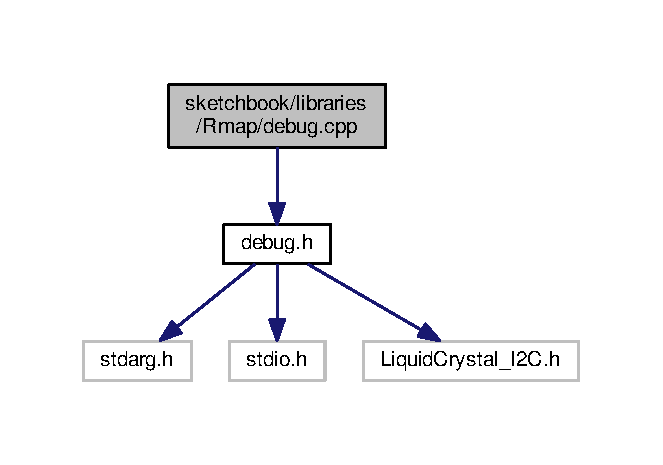
\includegraphics[width=318pt]{debug_8cpp__incl}
\end{center}
\end{figure}
\subsection*{Functions}
\begin{DoxyCompactItemize}
\item 
char $\ast$ \hyperlink{debug_8cpp_a9bcb9075bd69848b75520c3dcf0a54f3}{serial\+\_\+printf} (char $\ast$ptr, const char $\ast$fmt,...)
\begin{DoxyCompactList}\small\item\em Print a message over serial port preformatting it with a user defined values and parameters. \end{DoxyCompactList}\item 
char $\ast$ \hyperlink{debug_8cpp_a0e70d8336f97a77d525ae4c5b794c9e4}{serial\+\_\+printf} (char $\ast$ptr, const \+\_\+\+\_\+\+Flash\+String\+Helper $\ast$fmt,...)
\begin{DoxyCompactList}\small\item\em Print a message over serial port preformatting it with a user defined values and parameters. \end{DoxyCompactList}\item 
char $\ast$ \hyperlink{debug_8cpp_ab7517f3be15c21843ce73c609442bd30}{serial\+\_\+printf\+\_\+array} (void $\ast$data, int16\+\_\+t length, uint8\+\_\+t type, const \+\_\+\+\_\+\+Flash\+String\+Helper $\ast$fmt,...)
\begin{DoxyCompactList}\small\item\em Print array of data over serial port preformatting it with a user defined values and parameters. \end{DoxyCompactList}\item 
void \hyperlink{debug_8cpp_af5ec9e4b05706cb28aff868525e72d28}{lcd\+\_\+begin} (Liquid\+Crystal\+\_\+\+I2C $\ast$\hyperlink{rmap_8h_af7d08a33a932b4784cae528e8219f1c7}{lcd}, uint8\+\_\+t max\+\_\+cols, uint8\+\_\+t max\+\_\+rows)
\begin{DoxyCompactList}\small\item\em Initialize L\+CD library. \end{DoxyCompactList}\item 
char $\ast$ \hyperlink{debug_8cpp_a72c5742f32833defecbd437f12268776}{lcd\+\_\+printf} (Liquid\+Crystal\+\_\+\+I2C $\ast$\hyperlink{rmap_8h_af7d08a33a932b4784cae528e8219f1c7}{lcd}, bool do\+\_\+clear, bool go\+\_\+to\+\_\+next\+\_\+line, char $\ast$ptr, const char $\ast$fmt,...)
\begin{DoxyCompactList}\small\item\em Print a message on lcd preformatting it with a user defined values and parameters. \end{DoxyCompactList}\item 
char $\ast$ \hyperlink{debug_8cpp_a160bbf960a3f5defb1b84d4a0190dde9}{lcd\+\_\+printf} (Liquid\+Crystal\+\_\+\+I2C $\ast$\hyperlink{rmap_8h_af7d08a33a932b4784cae528e8219f1c7}{lcd}, bool do\+\_\+clear, bool go\+\_\+to\+\_\+next\+\_\+line, char $\ast$ptr, const \+\_\+\+\_\+\+Flash\+String\+Helper $\ast$fmt,...)
\begin{DoxyCompactList}\small\item\em Print a message on lcd preformatting it with a user defined values and parameters. \end{DoxyCompactList}\end{DoxyCompactItemize}
\subsection*{Variables}
\begin{DoxyCompactItemize}
\item 
\mbox{\Hypertarget{debug_8cpp_adc837429453017966fe21ec8fb429485}\label{debug_8cpp_adc837429453017966fe21ec8fb429485}} 
char \hyperlink{debug_8cpp_adc837429453017966fe21ec8fb429485}{serial\+\_\+buffer\+\_\+print} \mbox{[}\hyperlink{debug_8h_aaeec252c41b3be1d1bf272ce43b9b13f}{S\+E\+R\+I\+A\+L\+\_\+\+P\+R\+I\+N\+T\+F\+\_\+\+B\+U\+F\+F\+E\+R\+\_\+\+L\+E\+N\+G\+TH}\mbox{]}
\begin{DoxyCompactList}\small\item\em Serial data buffer for storing message before print. \end{DoxyCompactList}\item 
\mbox{\Hypertarget{debug_8cpp_a375e98fe7985a5396ab4e498726ba898}\label{debug_8cpp_a375e98fe7985a5396ab4e498726ba898}} 
int16\+\_\+t \hyperlink{debug_8cpp_a375e98fe7985a5396ab4e498726ba898}{serial\+\_\+buffer\+\_\+print\+\_\+written\+\_\+char}
\begin{DoxyCompactList}\small\item\em Length in bytes of serial data buffer. \end{DoxyCompactList}\item 
\mbox{\Hypertarget{debug_8cpp_a65fe8e6ffea87a3b13b06b44602a107f}\label{debug_8cpp_a65fe8e6ffea87a3b13b06b44602a107f}} 
char \hyperlink{debug_8cpp_a65fe8e6ffea87a3b13b06b44602a107f}{lcd\+\_\+buffer\+\_\+print} \mbox{[}\hyperlink{debug_8h_a05952bc8be9df24d159e158fa7e37aa9}{L\+C\+D\+\_\+\+P\+R\+I\+N\+T\+F\+\_\+\+B\+U\+F\+F\+E\+R\+\_\+\+L\+E\+N\+G\+TH}\mbox{]}
\begin{DoxyCompactList}\small\item\em Lcd data buffer for storing message before print. \end{DoxyCompactList}\item 
\mbox{\Hypertarget{debug_8cpp_a8e7c72370a12c8df2de628fe4e47d802}\label{debug_8cpp_a8e7c72370a12c8df2de628fe4e47d802}} 
uint8\+\_\+t \hyperlink{debug_8cpp_a8e7c72370a12c8df2de628fe4e47d802}{lcd\+\_\+current\+\_\+row}
\begin{DoxyCompactList}\small\item\em Indicate the \char`\"{}free to print\char`\"{} lcd row. \end{DoxyCompactList}\item 
\mbox{\Hypertarget{debug_8cpp_a3a35c553d138e96f0b2d5850d6a1f8d4}\label{debug_8cpp_a3a35c553d138e96f0b2d5850d6a1f8d4}} 
uint8\+\_\+t \hyperlink{debug_8cpp_a3a35c553d138e96f0b2d5850d6a1f8d4}{lcd\+\_\+max\+\_\+cols}
\begin{DoxyCompactList}\small\item\em Number of lcd columns. \end{DoxyCompactList}\item 
\mbox{\Hypertarget{debug_8cpp_a8a5985b489c245c2ff62a3a11e835f95}\label{debug_8cpp_a8a5985b489c245c2ff62a3a11e835f95}} 
uint8\+\_\+t \hyperlink{debug_8cpp_a8a5985b489c245c2ff62a3a11e835f95}{lcd\+\_\+max\+\_\+rows}
\begin{DoxyCompactList}\small\item\em Number of lcd rows. \end{DoxyCompactList}\end{DoxyCompactItemize}


\subsection{Function Documentation}
\mbox{\Hypertarget{debug_8cpp_af5ec9e4b05706cb28aff868525e72d28}\label{debug_8cpp_af5ec9e4b05706cb28aff868525e72d28}} 
\index{debug.\+cpp@{debug.\+cpp}!lcd\+\_\+begin@{lcd\+\_\+begin}}
\index{lcd\+\_\+begin@{lcd\+\_\+begin}!debug.\+cpp@{debug.\+cpp}}
\subsubsection{\texorpdfstring{lcd\+\_\+begin()}{lcd\_begin()}}
{\footnotesize\ttfamily void lcd\+\_\+begin (\begin{DoxyParamCaption}\item[{Liquid\+Crystal\+\_\+\+I2C $\ast$}]{lcd,  }\item[{uint8\+\_\+t}]{max\+\_\+cols,  }\item[{uint8\+\_\+t}]{max\+\_\+rows }\end{DoxyParamCaption})}



Initialize L\+CD library. 


\begin{DoxyParams}[1]{Parameters}
\mbox{\tt in}  & {\em $\ast$lcd} & pointer to lcd instance. \\
\hline
\mbox{\tt in}  & {\em max\+\_\+cols} & number of lcd columns. \\
\hline
\mbox{\tt in}  & {\em max\+\_\+rows} & number of lcd rows. \\
\hline
\end{DoxyParams}
\begin{DoxyReturn}{Returns}
void. 
\end{DoxyReturn}
\mbox{\Hypertarget{debug_8cpp_a72c5742f32833defecbd437f12268776}\label{debug_8cpp_a72c5742f32833defecbd437f12268776}} 
\index{debug.\+cpp@{debug.\+cpp}!lcd\+\_\+printf@{lcd\+\_\+printf}}
\index{lcd\+\_\+printf@{lcd\+\_\+printf}!debug.\+cpp@{debug.\+cpp}}
\subsubsection{\texorpdfstring{lcd\+\_\+printf()}{lcd\_printf()}\hspace{0.1cm}{\footnotesize\ttfamily [1/2]}}
{\footnotesize\ttfamily char $\ast$ lcd\+\_\+printf (\begin{DoxyParamCaption}\item[{Liquid\+Crystal\+\_\+\+I2C $\ast$}]{lcd,  }\item[{bool}]{do\+\_\+clear,  }\item[{bool}]{go\+\_\+to\+\_\+next\+\_\+line,  }\item[{char $\ast$}]{ptr,  }\item[{const char $\ast$}]{fmt,  }\item[{}]{... }\end{DoxyParamCaption})}



Print a message on lcd preformatting it with a user defined values and parameters. 


\begin{DoxyParams}[1]{Parameters}
\mbox{\tt in}  & {\em $\ast$lcd} & pointer to lcd instance. \\
\hline
\mbox{\tt in}  & {\em do\+\_\+clear} & if true, clear lcd before printing message \\
\hline
\mbox{\tt in}  & {\em go\+\_\+to\+\_\+next\+\_\+line} & if true, print message to next line \\
\hline
\mbox{\tt in}  & {\em $\ast$ptr} & message to print. \\
\hline
\mbox{\tt in}  & {\em $\ast$fmt} & typo for vsnprintf function. \\
\hline
\end{DoxyParams}
\begin{DoxyReturn}{Returns}
pointer to data buffer filled with message by vsnprintf function. 
\end{DoxyReturn}
\mbox{\Hypertarget{debug_8cpp_a160bbf960a3f5defb1b84d4a0190dde9}\label{debug_8cpp_a160bbf960a3f5defb1b84d4a0190dde9}} 
\index{debug.\+cpp@{debug.\+cpp}!lcd\+\_\+printf@{lcd\+\_\+printf}}
\index{lcd\+\_\+printf@{lcd\+\_\+printf}!debug.\+cpp@{debug.\+cpp}}
\subsubsection{\texorpdfstring{lcd\+\_\+printf()}{lcd\_printf()}\hspace{0.1cm}{\footnotesize\ttfamily [2/2]}}
{\footnotesize\ttfamily char $\ast$ lcd\+\_\+printf (\begin{DoxyParamCaption}\item[{Liquid\+Crystal\+\_\+\+I2C $\ast$}]{lcd,  }\item[{bool}]{do\+\_\+clear,  }\item[{bool}]{go\+\_\+to\+\_\+next\+\_\+line,  }\item[{char $\ast$}]{ptr,  }\item[{const \+\_\+\+\_\+\+Flash\+String\+Helper $\ast$}]{fmt,  }\item[{}]{... }\end{DoxyParamCaption})}



Print a message on lcd preformatting it with a user defined values and parameters. 


\begin{DoxyParams}[1]{Parameters}
\mbox{\tt in}  & {\em $\ast$lcd} & pointer to lcd instance. \\
\hline
\mbox{\tt in}  & {\em do\+\_\+clear} & if true, clear lcd before printing message \\
\hline
\mbox{\tt in}  & {\em go\+\_\+to\+\_\+next\+\_\+line} & if true, print message to next line \\
\hline
\mbox{\tt in}  & {\em $\ast$ptr} & message to print. \\
\hline
\mbox{\tt in}  & {\em $\ast$fmt} & typo progmem for vsnprintf function. \\
\hline
\end{DoxyParams}
\begin{DoxyReturn}{Returns}
pointer to data buffer filled with message by vsnprintf function. 
\end{DoxyReturn}
\mbox{\Hypertarget{debug_8cpp_a9bcb9075bd69848b75520c3dcf0a54f3}\label{debug_8cpp_a9bcb9075bd69848b75520c3dcf0a54f3}} 
\index{debug.\+cpp@{debug.\+cpp}!serial\+\_\+printf@{serial\+\_\+printf}}
\index{serial\+\_\+printf@{serial\+\_\+printf}!debug.\+cpp@{debug.\+cpp}}
\subsubsection{\texorpdfstring{serial\+\_\+printf()}{serial\_printf()}\hspace{0.1cm}{\footnotesize\ttfamily [1/2]}}
{\footnotesize\ttfamily char $\ast$ serial\+\_\+printf (\begin{DoxyParamCaption}\item[{char $\ast$}]{ptr,  }\item[{const char $\ast$}]{fmt,  }\item[{}]{... }\end{DoxyParamCaption})}



Print a message over serial port preformatting it with a user defined values and parameters. 


\begin{DoxyParams}[1]{Parameters}
\mbox{\tt in}  & {\em $\ast$ptr} & message to print. \\
\hline
\mbox{\tt in}  & {\em $\ast$fmt} & typo for vsnprintf function. \\
\hline
\end{DoxyParams}
\begin{DoxyReturn}{Returns}
pointer to data buffer filled with message by vsnprintf function. 
\end{DoxyReturn}
\mbox{\Hypertarget{debug_8cpp_a0e70d8336f97a77d525ae4c5b794c9e4}\label{debug_8cpp_a0e70d8336f97a77d525ae4c5b794c9e4}} 
\index{debug.\+cpp@{debug.\+cpp}!serial\+\_\+printf@{serial\+\_\+printf}}
\index{serial\+\_\+printf@{serial\+\_\+printf}!debug.\+cpp@{debug.\+cpp}}
\subsubsection{\texorpdfstring{serial\+\_\+printf()}{serial\_printf()}\hspace{0.1cm}{\footnotesize\ttfamily [2/2]}}
{\footnotesize\ttfamily char $\ast$ serial\+\_\+printf (\begin{DoxyParamCaption}\item[{char $\ast$}]{ptr,  }\item[{const \+\_\+\+\_\+\+Flash\+String\+Helper $\ast$}]{fmt,  }\item[{}]{... }\end{DoxyParamCaption})}



Print a message over serial port preformatting it with a user defined values and parameters. 


\begin{DoxyParams}[1]{Parameters}
\mbox{\tt in}  & {\em $\ast$ptr} & message to print. \\
\hline
\mbox{\tt in}  & {\em $\ast$fmt} & progmem for vsnprintf\+\_\+P function. \\
\hline
\end{DoxyParams}
\begin{DoxyReturn}{Returns}
pointer to data buffer filled with message by vsnprintf function. 
\end{DoxyReturn}
\mbox{\Hypertarget{debug_8cpp_ab7517f3be15c21843ce73c609442bd30}\label{debug_8cpp_ab7517f3be15c21843ce73c609442bd30}} 
\index{debug.\+cpp@{debug.\+cpp}!serial\+\_\+printf\+\_\+array@{serial\+\_\+printf\+\_\+array}}
\index{serial\+\_\+printf\+\_\+array@{serial\+\_\+printf\+\_\+array}!debug.\+cpp@{debug.\+cpp}}
\subsubsection{\texorpdfstring{serial\+\_\+printf\+\_\+array()}{serial\_printf\_array()}}
{\footnotesize\ttfamily char $\ast$ serial\+\_\+printf\+\_\+array (\begin{DoxyParamCaption}\item[{void $\ast$}]{data,  }\item[{int16\+\_\+t}]{length,  }\item[{uint8\+\_\+t}]{type,  }\item[{const \+\_\+\+\_\+\+Flash\+String\+Helper $\ast$}]{fmt,  }\item[{}]{... }\end{DoxyParamCaption})}



Print array of data over serial port preformatting it with a user defined values and parameters. 


\begin{DoxyParams}[1]{Parameters}
\mbox{\tt in}  & {\em $\ast$data} & array of data to print. \\
\hline
\mbox{\tt in}  & {\em length} & length of array \\
\hline
\mbox{\tt in}  & {\em type} & type of array elements for correct printing (specified by I\+N\+T8, I\+N\+T16, I\+N\+T32, U\+I\+N\+T8, U\+I\+N\+T16, U\+I\+N\+T32 defines) \\
\hline
\mbox{\tt in}  & {\em $\ast$fmt} & typo for vsnprintf function. \\
\hline
\end{DoxyParams}
\begin{DoxyReturn}{Returns}
pointer to data buffer filled with message by vsnprintf function. 
\end{DoxyReturn}

\hypertarget{debug_8h}{}\section{sketchbook/libraries/\+Rmap/debug.h File Reference}
\label{debug_8h}\index{sketchbook/libraries/\+Rmap/debug.\+h@{sketchbook/libraries/\+Rmap/debug.\+h}}
{\ttfamily \#include $<$stdarg.\+h$>$}\newline
{\ttfamily \#include $<$stdio.\+h$>$}\newline
{\ttfamily \#include $<$Liquid\+Crystal\+\_\+\+I2\+C.\+h$>$}\newline
Include dependency graph for debug.\+h\+:\nopagebreak
\begin{figure}[H]
\begin{center}
\leavevmode
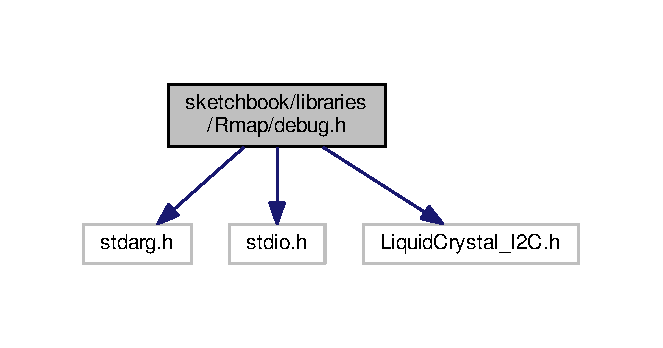
\includegraphics[width=318pt]{debug_8h__incl}
\end{center}
\end{figure}
This graph shows which files directly or indirectly include this file\+:\nopagebreak
\begin{figure}[H]
\begin{center}
\leavevmode
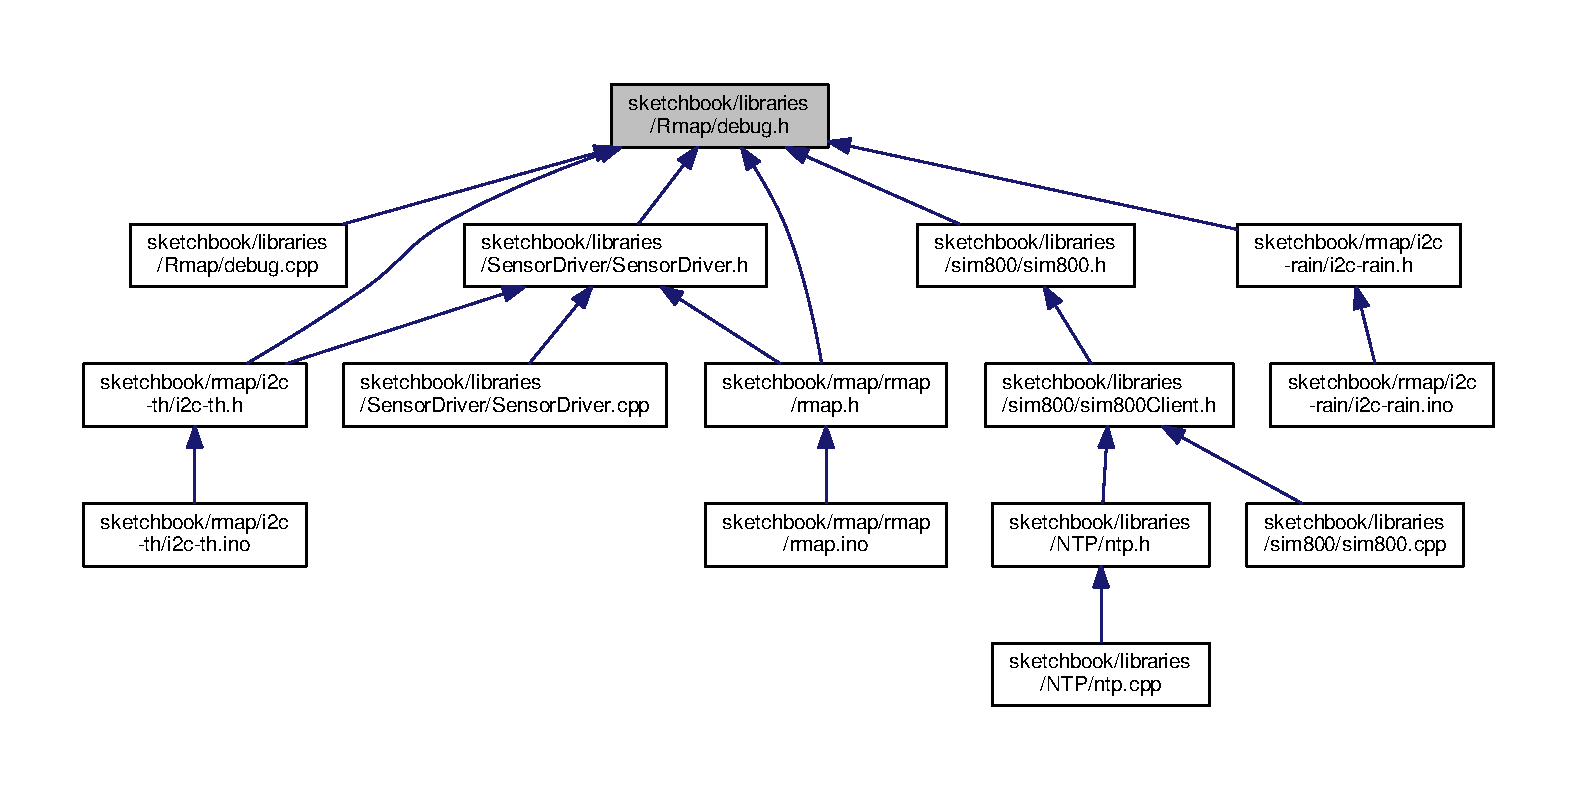
\includegraphics[width=350pt]{debug_8h__dep__incl}
\end{center}
\end{figure}
\subsection*{Macros}
\begin{DoxyCompactItemize}
\item 
\mbox{\Hypertarget{debug_8h_a7e125472d65b57f10905accbed140b99}\label{debug_8h_a7e125472d65b57f10905accbed140b99}} 
\#define \hyperlink{debug_8h_a7e125472d65b57f10905accbed140b99}{I\+N\+T8}~(1)
\begin{DoxyCompactList}\small\item\em Indicate a int8\+\_\+t type. \end{DoxyCompactList}\item 
\mbox{\Hypertarget{debug_8h_abc743ce126c3ada10501baffb3ca2295}\label{debug_8h_abc743ce126c3ada10501baffb3ca2295}} 
\#define \hyperlink{debug_8h_abc743ce126c3ada10501baffb3ca2295}{I\+N\+T16}~(2)
\begin{DoxyCompactList}\small\item\em Indicate a int16\+\_\+t type. \end{DoxyCompactList}\item 
\mbox{\Hypertarget{debug_8h_aac92c5ec332dafe0abb24688dad1b795}\label{debug_8h_aac92c5ec332dafe0abb24688dad1b795}} 
\#define \hyperlink{debug_8h_aac92c5ec332dafe0abb24688dad1b795}{I\+N\+T32}~(3)
\begin{DoxyCompactList}\small\item\em Indicate a int32\+\_\+t type. \end{DoxyCompactList}\item 
\mbox{\Hypertarget{debug_8h_ad8ce12d83f204245685f98caf9d03944}\label{debug_8h_ad8ce12d83f204245685f98caf9d03944}} 
\#define \hyperlink{debug_8h_ad8ce12d83f204245685f98caf9d03944}{U\+I\+N\+T8}~(4)
\begin{DoxyCompactList}\small\item\em Indicate a uint8\+\_\+t type. \end{DoxyCompactList}\item 
\mbox{\Hypertarget{debug_8h_ab1922c2d8643eb7da964d427604e992e}\label{debug_8h_ab1922c2d8643eb7da964d427604e992e}} 
\#define \hyperlink{debug_8h_ab1922c2d8643eb7da964d427604e992e}{U\+I\+N\+T16}~(5)
\begin{DoxyCompactList}\small\item\em Indicate a uint16\+\_\+t type. \end{DoxyCompactList}\item 
\mbox{\Hypertarget{debug_8h_a69afa2e50b905f4eab1f2df8a3fd9f23}\label{debug_8h_a69afa2e50b905f4eab1f2df8a3fd9f23}} 
\#define \hyperlink{debug_8h_a69afa2e50b905f4eab1f2df8a3fd9f23}{U\+I\+N\+T32}~(6)
\begin{DoxyCompactList}\small\item\em Indicate a uint32\+\_\+t type. \end{DoxyCompactList}\item 
\mbox{\Hypertarget{debug_8h_ae8690abbffa85934d64d545920e2b108}\label{debug_8h_ae8690abbffa85934d64d545920e2b108}} 
\#define \hyperlink{debug_8h_ae8690abbffa85934d64d545920e2b108}{F\+L\+O\+AT}~(7)
\begin{DoxyCompactList}\small\item\em Indicate a float type. \end{DoxyCompactList}\item 
\mbox{\Hypertarget{debug_8h_a29b98fcac07224e9d92c51cfed5fc0e6}\label{debug_8h_a29b98fcac07224e9d92c51cfed5fc0e6}} 
\#define \hyperlink{debug_8h_a29b98fcac07224e9d92c51cfed5fc0e6}{D\+E\+B\+U\+G\+\_\+\+W\+A\+I\+T\+\_\+\+F\+O\+R\+\_\+\+S\+L\+E\+E\+P\+\_\+\+MS}~(10)
\begin{DoxyCompactList}\small\item\em If power down mode is enable, a necessary delay was needed after a debug message for correct print. \end{DoxyCompactList}\item 
\mbox{\Hypertarget{debug_8h_aaeec252c41b3be1d1bf272ce43b9b13f}\label{debug_8h_aaeec252c41b3be1d1bf272ce43b9b13f}} 
\#define \hyperlink{debug_8h_aaeec252c41b3be1d1bf272ce43b9b13f}{S\+E\+R\+I\+A\+L\+\_\+\+P\+R\+I\+N\+T\+F\+\_\+\+B\+U\+F\+F\+E\+R\+\_\+\+L\+E\+N\+G\+TH}~(256)
\begin{DoxyCompactList}\small\item\em Length in bytes for serial data buffer. \end{DoxyCompactList}\item 
\mbox{\Hypertarget{debug_8h_a05952bc8be9df24d159e158fa7e37aa9}\label{debug_8h_a05952bc8be9df24d159e158fa7e37aa9}} 
\#define \hyperlink{debug_8h_a05952bc8be9df24d159e158fa7e37aa9}{L\+C\+D\+\_\+\+P\+R\+I\+N\+T\+F\+\_\+\+B\+U\+F\+F\+E\+R\+\_\+\+L\+E\+N\+G\+TH}~(20)
\begin{DoxyCompactList}\small\item\em Length in bytes for lcd data buffer. \end{DoxyCompactList}\item 
\mbox{\Hypertarget{debug_8h_a31fa5c36fa17c66feec7a67b76c3e786}\label{debug_8h_a31fa5c36fa17c66feec7a67b76c3e786}} 
\#define \hyperlink{debug_8h_a31fa5c36fa17c66feec7a67b76c3e786}{S\+E\+R\+I\+A\+L\+\_\+\+T\+R\+A\+C\+E\+\_\+\+L\+E\+V\+EL}~\hyperlink{debug__config_8h_ab6322e7dccbadeed1a84b6e4b5eba819}{S\+E\+R\+I\+A\+L\+\_\+\+T\+R\+A\+C\+E\+\_\+\+L\+E\+V\+E\+L\+\_\+\+O\+FF}
\begin{DoxyCompactList}\small\item\em Serial trace level is disable for default. \end{DoxyCompactList}\item 
\mbox{\Hypertarget{debug_8h_a03011829badde0371233790daf8dbd34}\label{debug_8h_a03011829badde0371233790daf8dbd34}} 
\#define \hyperlink{debug_8h_a03011829badde0371233790daf8dbd34}{S\+E\+R\+I\+A\+L\+\_\+\+B\+E\+G\+IN}(...)
\begin{DoxyCompactList}\small\item\em If serial debug was disabled, this macro do nothing. \end{DoxyCompactList}\item 
\mbox{\Hypertarget{debug_8h_a640002baf58b6a49613e7ccde361357a}\label{debug_8h_a640002baf58b6a49613e7ccde361357a}} 
\#define \hyperlink{debug_8h_a640002baf58b6a49613e7ccde361357a}{S\+E\+R\+I\+A\+L\+\_\+\+E\+R\+R\+OR}(...)~\+\_\+\+S\+E\+R\+I\+A\+L\+\_\+\+P\+R\+I\+NT(N\+U\+LL, \+\_\+\+\_\+\+V\+A\+\_\+\+A\+R\+G\+S\+\_\+\+\_\+)
\begin{DoxyCompactList}\small\item\em Useful macro for print error message on serial port through serial print macro. \end{DoxyCompactList}\item 
\mbox{\Hypertarget{debug_8h_ae8414f64d262e02dd90240a1e3e81c9b}\label{debug_8h_ae8414f64d262e02dd90240a1e3e81c9b}} 
\#define \hyperlink{debug_8h_ae8414f64d262e02dd90240a1e3e81c9b}{S\+E\+R\+I\+A\+L\+\_\+\+E\+R\+R\+O\+R\+\_\+\+A\+R\+R\+AY}(...)~\+\_\+\+S\+E\+R\+I\+A\+L\+\_\+\+P\+R\+I\+N\+T\+\_\+\+A\+R\+R\+AY(\+\_\+\+\_\+\+V\+A\+\_\+\+A\+R\+G\+S\+\_\+\+\_\+)
\begin{DoxyCompactList}\small\item\em Useful macro for print array error message on serial port through serial print macro. \end{DoxyCompactList}\item 
\mbox{\Hypertarget{debug_8h_adaf8c9472cded6ccce35de9bbe5e58d7}\label{debug_8h_adaf8c9472cded6ccce35de9bbe5e58d7}} 
\#define \hyperlink{debug_8h_adaf8c9472cded6ccce35de9bbe5e58d7}{S\+E\+R\+I\+A\+L\+\_\+\+W\+A\+R\+N\+I\+NG}(...)~\+\_\+\+S\+E\+R\+I\+A\+L\+\_\+\+P\+R\+I\+NT(N\+U\+LL, \+\_\+\+\_\+\+V\+A\+\_\+\+A\+R\+G\+S\+\_\+\+\_\+)
\begin{DoxyCompactList}\small\item\em Useful macro for print warning message on serial port through serial print macro. \end{DoxyCompactList}\item 
\mbox{\Hypertarget{debug_8h_a88786fa81c01cbd6b3d23db370ae8c56}\label{debug_8h_a88786fa81c01cbd6b3d23db370ae8c56}} 
\#define \hyperlink{debug_8h_a88786fa81c01cbd6b3d23db370ae8c56}{S\+E\+R\+I\+A\+L\+\_\+\+W\+A\+R\+N\+I\+N\+G\+\_\+\+A\+R\+R\+AY}(...)~\+\_\+\+S\+E\+R\+I\+A\+L\+\_\+\+P\+R\+I\+N\+T\+\_\+\+A\+R\+R\+AY(\+\_\+\+\_\+\+V\+A\+\_\+\+A\+R\+G\+S\+\_\+\+\_\+)
\begin{DoxyCompactList}\small\item\em Useful macro for print warning array error message on serial port through serial print macro. \end{DoxyCompactList}\item 
\mbox{\Hypertarget{debug_8h_af211c01186da8b757a0921c0452dbfa6}\label{debug_8h_af211c01186da8b757a0921c0452dbfa6}} 
\#define \hyperlink{debug_8h_af211c01186da8b757a0921c0452dbfa6}{S\+E\+R\+I\+A\+L\+\_\+\+I\+N\+FO}(...)~\+\_\+\+S\+E\+R\+I\+A\+L\+\_\+\+P\+R\+I\+NT(N\+U\+LL, \+\_\+\+\_\+\+V\+A\+\_\+\+A\+R\+G\+S\+\_\+\+\_\+)
\begin{DoxyCompactList}\small\item\em Useful macro for print info message on serial port through serial print macro. \end{DoxyCompactList}\item 
\mbox{\Hypertarget{debug_8h_af87b98474a3dd17abcdaa43ddc463152}\label{debug_8h_af87b98474a3dd17abcdaa43ddc463152}} 
\#define \hyperlink{debug_8h_af87b98474a3dd17abcdaa43ddc463152}{S\+E\+R\+I\+A\+L\+\_\+\+I\+N\+F\+O\+\_\+\+A\+R\+R\+AY}(...)~\+\_\+\+S\+E\+R\+I\+A\+L\+\_\+\+P\+R\+I\+N\+T\+\_\+\+A\+R\+R\+AY(\+\_\+\+\_\+\+V\+A\+\_\+\+A\+R\+G\+S\+\_\+\+\_\+)
\begin{DoxyCompactList}\small\item\em Useful macro for print info array error message on serial port through serial print macro. \end{DoxyCompactList}\item 
\mbox{\Hypertarget{debug_8h_a31b291f78b1470a777a26c1ef53ad7c5}\label{debug_8h_a31b291f78b1470a777a26c1ef53ad7c5}} 
\#define \hyperlink{debug_8h_a31b291f78b1470a777a26c1ef53ad7c5}{S\+E\+R\+I\+A\+L\+\_\+\+D\+E\+B\+UG}(...)~\+\_\+\+S\+E\+R\+I\+A\+L\+\_\+\+P\+R\+I\+NT(N\+U\+LL, \+\_\+\+\_\+\+V\+A\+\_\+\+A\+R\+G\+S\+\_\+\+\_\+)
\begin{DoxyCompactList}\small\item\em Useful macro for print verbose message on serial port through serial print macro. \end{DoxyCompactList}\item 
\mbox{\Hypertarget{debug_8h_af2fff35f0152a2839d21d4c838904fca}\label{debug_8h_af2fff35f0152a2839d21d4c838904fca}} 
\#define \hyperlink{debug_8h_af2fff35f0152a2839d21d4c838904fca}{S\+E\+R\+I\+A\+L\+\_\+\+D\+E\+B\+U\+G\+\_\+\+A\+R\+R\+AY}(...)~\+\_\+\+S\+E\+R\+I\+A\+L\+\_\+\+P\+R\+I\+N\+T\+\_\+\+A\+R\+R\+AY(\+\_\+\+\_\+\+V\+A\+\_\+\+A\+R\+G\+S\+\_\+\+\_\+)
\begin{DoxyCompactList}\small\item\em Useful macro for print verbose array error message on serial port through serial print macro. \end{DoxyCompactList}\item 
\mbox{\Hypertarget{debug_8h_ab4302572ca631f772801a7742347deb1}\label{debug_8h_ab4302572ca631f772801a7742347deb1}} 
\#define \hyperlink{debug_8h_ab4302572ca631f772801a7742347deb1}{S\+E\+R\+I\+A\+L\+\_\+\+T\+R\+A\+CE}(...)~\+\_\+\+S\+E\+R\+I\+A\+L\+\_\+\+P\+R\+I\+NT(N\+U\+LL, \+\_\+\+\_\+\+V\+A\+\_\+\+A\+R\+G\+S\+\_\+\+\_\+)
\begin{DoxyCompactList}\small\item\em Useful macro for print all verbose message on serial port through serial print macro. \end{DoxyCompactList}\item 
\mbox{\Hypertarget{debug_8h_ac73a903b423d9925e298732c299d946b}\label{debug_8h_ac73a903b423d9925e298732c299d946b}} 
\#define \hyperlink{debug_8h_ac73a903b423d9925e298732c299d946b}{S\+E\+R\+I\+A\+L\+\_\+\+T\+R\+A\+C\+E\+\_\+\+A\+R\+R\+AY}(...)~\+\_\+\+S\+E\+R\+I\+A\+L\+\_\+\+P\+R\+I\+N\+T\+\_\+\+A\+R\+R\+AY(\+\_\+\+\_\+\+V\+A\+\_\+\+A\+R\+G\+S\+\_\+\+\_\+)
\begin{DoxyCompactList}\small\item\em Useful macro for print all verbose array error message on serial port through serial print macro. \end{DoxyCompactList}\item 
\mbox{\Hypertarget{debug_8h_acb771fe8deeaa2fee1ad327c0c1be34f}\label{debug_8h_acb771fe8deeaa2fee1ad327c0c1be34f}} 
\#define \hyperlink{debug_8h_acb771fe8deeaa2fee1ad327c0c1be34f}{L\+C\+D\+\_\+\+T\+R\+A\+C\+E\+\_\+\+L\+E\+V\+EL}~\hyperlink{debug__config_8h_ab40fd4608517cbf6acb6d6d369f43253}{L\+C\+D\+\_\+\+T\+R\+A\+C\+E\+\_\+\+L\+E\+V\+E\+L\+\_\+\+O\+FF}
\begin{DoxyCompactList}\small\item\em Lcd trace level is disable for default. \end{DoxyCompactList}\item 
\mbox{\Hypertarget{debug_8h_a2e398ce3ec4505784983cfdd9fd92952}\label{debug_8h_a2e398ce3ec4505784983cfdd9fd92952}} 
\#define \hyperlink{debug_8h_a2e398ce3ec4505784983cfdd9fd92952}{L\+C\+D\+\_\+\+B\+E\+G\+IN}(...)
\begin{DoxyCompactList}\small\item\em Useful macro for initialize lcd library. \end{DoxyCompactList}\item 
\mbox{\Hypertarget{debug_8h_a5132a5db535debb49fbe83393986fec0}\label{debug_8h_a5132a5db535debb49fbe83393986fec0}} 
\#define \hyperlink{debug_8h_a5132a5db535debb49fbe83393986fec0}{L\+C\+D\+\_\+\+E\+R\+R\+OR}(...)~\+\_\+\+L\+C\+D\+\_\+\+P\+R\+I\+NT(\+\_\+\+\_\+\+V\+A\+\_\+\+A\+R\+G\+S\+\_\+\+\_\+)
\begin{DoxyCompactList}\small\item\em Useful macro for print error message on lcd port through lcd print macro. \end{DoxyCompactList}\item 
\mbox{\Hypertarget{debug_8h_a94aa136503f794a227b75ed3cd4a1982}\label{debug_8h_a94aa136503f794a227b75ed3cd4a1982}} 
\#define \hyperlink{debug_8h_a94aa136503f794a227b75ed3cd4a1982}{L\+C\+D\+\_\+\+W\+A\+R\+N\+I\+NG}(...)~\+\_\+\+L\+C\+D\+\_\+\+P\+R\+I\+NT( \+\_\+\+\_\+\+V\+A\+\_\+\+A\+R\+G\+S\+\_\+\+\_\+)
\begin{DoxyCompactList}\small\item\em Useful macro for print warning message on lcd port through lcd print macro. \end{DoxyCompactList}\item 
\mbox{\Hypertarget{debug_8h_aae2acb78c87bcf0a1cc4d743c35efce9}\label{debug_8h_aae2acb78c87bcf0a1cc4d743c35efce9}} 
\#define \hyperlink{debug_8h_aae2acb78c87bcf0a1cc4d743c35efce9}{L\+C\+D\+\_\+\+I\+N\+FO}(...)~\+\_\+\+L\+C\+D\+\_\+\+P\+R\+I\+NT(\+\_\+\+\_\+\+V\+A\+\_\+\+A\+R\+G\+S\+\_\+\+\_\+)
\begin{DoxyCompactList}\small\item\em Useful macro for print info message on lcd port through lcd print macro. \end{DoxyCompactList}\item 
\mbox{\Hypertarget{debug_8h_a5e8434ef334222b3659115f760e1ecc8}\label{debug_8h_a5e8434ef334222b3659115f760e1ecc8}} 
\#define \hyperlink{debug_8h_a5e8434ef334222b3659115f760e1ecc8}{L\+C\+D\+\_\+\+D\+E\+B\+UG}(...)~\+\_\+\+L\+C\+D\+\_\+\+P\+R\+I\+NT( \+\_\+\+\_\+\+V\+A\+\_\+\+A\+R\+G\+S\+\_\+\+\_\+)
\begin{DoxyCompactList}\small\item\em Useful macro for print verbose message on lcd port through lcd print macro. \end{DoxyCompactList}\end{DoxyCompactItemize}
\subsection*{Functions}
\begin{DoxyCompactItemize}
\item 
char $\ast$ \hyperlink{debug_8h_aa6e7889d3df8dce23e626b0e00925ed5}{serial\+\_\+printf} (char $\ast$ptr, const char $\ast$fmt,...)
\begin{DoxyCompactList}\small\item\em Print a message over serial port preformatting it with a user defined values and parameters. \end{DoxyCompactList}\item 
char $\ast$ \hyperlink{debug_8h_aeb1c209d589a4799fa4e1fc3f14cb77e}{serial\+\_\+printf} (char $\ast$ptr, const \+\_\+\+\_\+\+Flash\+String\+Helper $\ast$fmt,...)
\begin{DoxyCompactList}\small\item\em Print a message over serial port preformatting it with a user defined values and parameters. \end{DoxyCompactList}\item 
char $\ast$ \hyperlink{debug_8h_a3b747bc953d57217b1f940a05cdb4caf}{serial\+\_\+printf\+\_\+array} (void $\ast$data, int16\+\_\+t length, uint8\+\_\+t type, const \+\_\+\+\_\+\+Flash\+String\+Helper $\ast$fmt,...)
\begin{DoxyCompactList}\small\item\em Print array of data over serial port preformatting it with a user defined values and parameters. \end{DoxyCompactList}\item 
void \hyperlink{debug_8h_af5ec9e4b05706cb28aff868525e72d28}{lcd\+\_\+begin} (Liquid\+Crystal\+\_\+\+I2C $\ast$\hyperlink{rmap_8h_af7d08a33a932b4784cae528e8219f1c7}{lcd}, uint8\+\_\+t max\+\_\+cols, uint8\+\_\+t max\+\_\+rows)
\begin{DoxyCompactList}\small\item\em Initialize L\+CD library. \end{DoxyCompactList}\item 
char $\ast$ \hyperlink{debug_8h_ae47a9edd316c68d2030312d22dd670e3}{lcd\+\_\+printf} (Liquid\+Crystal\+\_\+\+I2C $\ast$\hyperlink{rmap_8h_af7d08a33a932b4784cae528e8219f1c7}{lcd}, bool do\+\_\+clear, bool go\+\_\+to\+\_\+next\+\_\+line, char $\ast$ptr, const \+\_\+\+\_\+\+Flash\+String\+Helper $\ast$fmt,...)
\begin{DoxyCompactList}\small\item\em Print a message on lcd preformatting it with a user defined values and parameters. \end{DoxyCompactList}\item 
char $\ast$ \hyperlink{debug_8h_a7b3b66011772f8225cfa3a545841d6d3}{lcd\+\_\+printf} (Liquid\+Crystal\+\_\+\+I2C $\ast$\hyperlink{rmap_8h_af7d08a33a932b4784cae528e8219f1c7}{lcd}, bool do\+\_\+clear, bool go\+\_\+to\+\_\+next\+\_\+line, char $\ast$ptr, const char $\ast$fmt,...)
\begin{DoxyCompactList}\small\item\em Print a message on lcd preformatting it with a user defined values and parameters. \end{DoxyCompactList}\end{DoxyCompactItemize}


\subsection{Function Documentation}
\mbox{\Hypertarget{debug_8h_af5ec9e4b05706cb28aff868525e72d28}\label{debug_8h_af5ec9e4b05706cb28aff868525e72d28}} 
\index{debug.\+h@{debug.\+h}!lcd\+\_\+begin@{lcd\+\_\+begin}}
\index{lcd\+\_\+begin@{lcd\+\_\+begin}!debug.\+h@{debug.\+h}}
\subsubsection{\texorpdfstring{lcd\+\_\+begin()}{lcd\_begin()}}
{\footnotesize\ttfamily void lcd\+\_\+begin (\begin{DoxyParamCaption}\item[{Liquid\+Crystal\+\_\+\+I2C $\ast$}]{lcd,  }\item[{uint8\+\_\+t}]{max\+\_\+cols,  }\item[{uint8\+\_\+t}]{max\+\_\+rows }\end{DoxyParamCaption})}



Initialize L\+CD library. 


\begin{DoxyParams}[1]{Parameters}
\mbox{\tt in}  & {\em $\ast$lcd} & pointer to lcd instance. \\
\hline
\mbox{\tt in}  & {\em max\+\_\+cols} & number of lcd columns. \\
\hline
\mbox{\tt in}  & {\em max\+\_\+rows} & number of lcd rows. \\
\hline
\end{DoxyParams}
\begin{DoxyReturn}{Returns}
void. 
\end{DoxyReturn}
\mbox{\Hypertarget{debug_8h_ae47a9edd316c68d2030312d22dd670e3}\label{debug_8h_ae47a9edd316c68d2030312d22dd670e3}} 
\index{debug.\+h@{debug.\+h}!lcd\+\_\+printf@{lcd\+\_\+printf}}
\index{lcd\+\_\+printf@{lcd\+\_\+printf}!debug.\+h@{debug.\+h}}
\subsubsection{\texorpdfstring{lcd\+\_\+printf()}{lcd\_printf()}\hspace{0.1cm}{\footnotesize\ttfamily [1/2]}}
{\footnotesize\ttfamily char$\ast$ lcd\+\_\+printf (\begin{DoxyParamCaption}\item[{Liquid\+Crystal\+\_\+\+I2C $\ast$}]{lcd,  }\item[{bool}]{do\+\_\+clear,  }\item[{bool}]{go\+\_\+to\+\_\+next\+\_\+line,  }\item[{char $\ast$}]{ptr,  }\item[{const \+\_\+\+\_\+\+Flash\+String\+Helper $\ast$}]{fmt,  }\item[{}]{... }\end{DoxyParamCaption})}



Print a message on lcd preformatting it with a user defined values and parameters. 


\begin{DoxyParams}[1]{Parameters}
\mbox{\tt in}  & {\em $\ast$lcd} & pointer to lcd instance. \\
\hline
\mbox{\tt in}  & {\em do\+\_\+clear} & if true, clear lcd before printing message \\
\hline
\mbox{\tt in}  & {\em go\+\_\+to\+\_\+next\+\_\+line} & if true, print message to next line \\
\hline
\mbox{\tt in}  & {\em $\ast$ptr} & message to print. \\
\hline
\mbox{\tt in}  & {\em $\ast$fmt} & typo progmem for vsnprintf function. \\
\hline
\end{DoxyParams}
\begin{DoxyReturn}{Returns}
pointer to data buffer filled with message by vsnprintf function. 
\end{DoxyReturn}
\mbox{\Hypertarget{debug_8h_a7b3b66011772f8225cfa3a545841d6d3}\label{debug_8h_a7b3b66011772f8225cfa3a545841d6d3}} 
\index{debug.\+h@{debug.\+h}!lcd\+\_\+printf@{lcd\+\_\+printf}}
\index{lcd\+\_\+printf@{lcd\+\_\+printf}!debug.\+h@{debug.\+h}}
\subsubsection{\texorpdfstring{lcd\+\_\+printf()}{lcd\_printf()}\hspace{0.1cm}{\footnotesize\ttfamily [2/2]}}
{\footnotesize\ttfamily char$\ast$ lcd\+\_\+printf (\begin{DoxyParamCaption}\item[{Liquid\+Crystal\+\_\+\+I2C $\ast$}]{lcd,  }\item[{bool}]{do\+\_\+clear,  }\item[{bool}]{go\+\_\+to\+\_\+next\+\_\+line,  }\item[{char $\ast$}]{ptr,  }\item[{const char $\ast$}]{fmt,  }\item[{}]{... }\end{DoxyParamCaption})}



Print a message on lcd preformatting it with a user defined values and parameters. 


\begin{DoxyParams}[1]{Parameters}
\mbox{\tt in}  & {\em $\ast$lcd} & pointer to lcd instance. \\
\hline
\mbox{\tt in}  & {\em do\+\_\+clear} & if true, clear lcd before printing message \\
\hline
\mbox{\tt in}  & {\em go\+\_\+to\+\_\+next\+\_\+line} & if true, print message to next line \\
\hline
\mbox{\tt in}  & {\em $\ast$ptr} & message to print. \\
\hline
\mbox{\tt in}  & {\em $\ast$fmt} & typo for vsnprintf function. \\
\hline
\end{DoxyParams}
\begin{DoxyReturn}{Returns}
pointer to data buffer filled with message by vsnprintf function. 
\end{DoxyReturn}
\mbox{\Hypertarget{debug_8h_aa6e7889d3df8dce23e626b0e00925ed5}\label{debug_8h_aa6e7889d3df8dce23e626b0e00925ed5}} 
\index{debug.\+h@{debug.\+h}!serial\+\_\+printf@{serial\+\_\+printf}}
\index{serial\+\_\+printf@{serial\+\_\+printf}!debug.\+h@{debug.\+h}}
\subsubsection{\texorpdfstring{serial\+\_\+printf()}{serial\_printf()}\hspace{0.1cm}{\footnotesize\ttfamily [1/2]}}
{\footnotesize\ttfamily char$\ast$ serial\+\_\+printf (\begin{DoxyParamCaption}\item[{char $\ast$}]{ptr,  }\item[{const char $\ast$}]{fmt,  }\item[{}]{... }\end{DoxyParamCaption})}



Print a message over serial port preformatting it with a user defined values and parameters. 


\begin{DoxyParams}[1]{Parameters}
\mbox{\tt in}  & {\em $\ast$ptr} & message to print. \\
\hline
\mbox{\tt in}  & {\em $\ast$fmt} & typo for vsnprintf function. \\
\hline
\end{DoxyParams}
\begin{DoxyReturn}{Returns}
pointer to data buffer filled with message by vsnprintf function. 
\end{DoxyReturn}
\mbox{\Hypertarget{debug_8h_aeb1c209d589a4799fa4e1fc3f14cb77e}\label{debug_8h_aeb1c209d589a4799fa4e1fc3f14cb77e}} 
\index{debug.\+h@{debug.\+h}!serial\+\_\+printf@{serial\+\_\+printf}}
\index{serial\+\_\+printf@{serial\+\_\+printf}!debug.\+h@{debug.\+h}}
\subsubsection{\texorpdfstring{serial\+\_\+printf()}{serial\_printf()}\hspace{0.1cm}{\footnotesize\ttfamily [2/2]}}
{\footnotesize\ttfamily char$\ast$ serial\+\_\+printf (\begin{DoxyParamCaption}\item[{char $\ast$}]{ptr,  }\item[{const \+\_\+\+\_\+\+Flash\+String\+Helper $\ast$}]{fmt,  }\item[{}]{... }\end{DoxyParamCaption})}



Print a message over serial port preformatting it with a user defined values and parameters. 


\begin{DoxyParams}[1]{Parameters}
\mbox{\tt in}  & {\em $\ast$ptr} & message to print. \\
\hline
\mbox{\tt in}  & {\em $\ast$fmt} & progmem for vsnprintf\+\_\+P function. \\
\hline
\end{DoxyParams}
\begin{DoxyReturn}{Returns}
pointer to data buffer filled with message by vsnprintf function. 
\end{DoxyReturn}
\mbox{\Hypertarget{debug_8h_a3b747bc953d57217b1f940a05cdb4caf}\label{debug_8h_a3b747bc953d57217b1f940a05cdb4caf}} 
\index{debug.\+h@{debug.\+h}!serial\+\_\+printf\+\_\+array@{serial\+\_\+printf\+\_\+array}}
\index{serial\+\_\+printf\+\_\+array@{serial\+\_\+printf\+\_\+array}!debug.\+h@{debug.\+h}}
\subsubsection{\texorpdfstring{serial\+\_\+printf\+\_\+array()}{serial\_printf\_array()}}
{\footnotesize\ttfamily char$\ast$ serial\+\_\+printf\+\_\+array (\begin{DoxyParamCaption}\item[{void $\ast$}]{data,  }\item[{int16\+\_\+t}]{length,  }\item[{uint8\+\_\+t}]{type,  }\item[{const \+\_\+\+\_\+\+Flash\+String\+Helper $\ast$}]{fmt,  }\item[{}]{... }\end{DoxyParamCaption})}



Print array of data over serial port preformatting it with a user defined values and parameters. 


\begin{DoxyParams}[1]{Parameters}
\mbox{\tt in}  & {\em $\ast$data} & array of data to print. \\
\hline
\mbox{\tt in}  & {\em length} & length of array \\
\hline
\mbox{\tt in}  & {\em type} & type of array elements for correct printing (specified by I\+N\+T8, I\+N\+T16, I\+N\+T32, U\+I\+N\+T8, U\+I\+N\+T16, U\+I\+N\+T32 defines) \\
\hline
\mbox{\tt in}  & {\em $\ast$fmt} & typo for vsnprintf function. \\
\hline
\end{DoxyParams}
\begin{DoxyReturn}{Returns}
pointer to data buffer filled with message by vsnprintf function. 
\end{DoxyReturn}

\hypertarget{eeprom__utility_8h}{}\section{sketchbook/libraries/\+Rmap/eeprom\+\_\+utility.h File Reference}
\label{eeprom__utility_8h}\index{sketchbook/libraries/\+Rmap/eeprom\+\_\+utility.\+h@{sketchbook/libraries/\+Rmap/eeprom\+\_\+utility.\+h}}
{\ttfamily \#include $<$avr/eeprom.\+h$>$}\newline
Include dependency graph for eeprom\+\_\+utility.\+h\+:\nopagebreak
\begin{figure}[H]
\begin{center}
\leavevmode
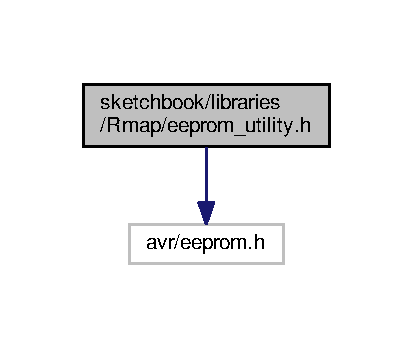
\includegraphics[width=198pt]{eeprom__utility_8h__incl}
\end{center}
\end{figure}
This graph shows which files directly or indirectly include this file\+:\nopagebreak
\begin{figure}[H]
\begin{center}
\leavevmode
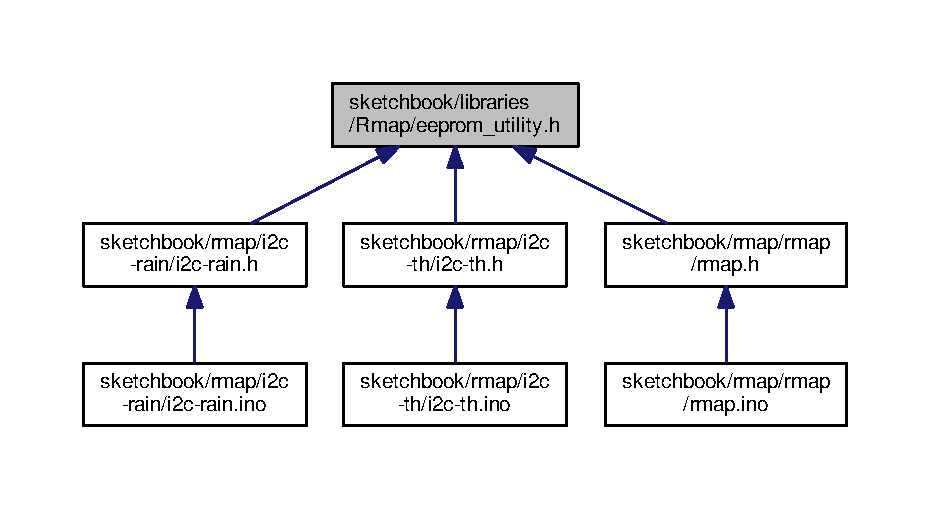
\includegraphics[width=350pt]{eeprom__utility_8h__dep__incl}
\end{center}
\end{figure}
\subsection*{Macros}
\begin{DoxyCompactItemize}
\item 
\mbox{\Hypertarget{eeprom__utility_8h_a715dca2643f9f8ee01f6ea0f484be62e}\label{eeprom__utility_8h_a715dca2643f9f8ee01f6ea0f484be62e}} 
\#define \hyperlink{eeprom__utility_8h_a715dca2643f9f8ee01f6ea0f484be62e}{ee\+\_\+read}(data,  address,  size)~(eeprom\+\_\+read\+\_\+block((void $\ast$)data, (const void $\ast$)address, size))
\begin{DoxyCompactList}\small\item\em Read size bytes of data in eeprom at specified address. \end{DoxyCompactList}\item 
\mbox{\Hypertarget{eeprom__utility_8h_afa92ea9ce29595f99960fe4c0dc3cda9}\label{eeprom__utility_8h_afa92ea9ce29595f99960fe4c0dc3cda9}} 
\#define \hyperlink{eeprom__utility_8h_afa92ea9ce29595f99960fe4c0dc3cda9}{ee\+\_\+write}(data,  address,  size)~(eeprom\+\_\+write\+\_\+block((void $\ast$)data, (void $\ast$)address, size))
\begin{DoxyCompactList}\small\item\em Write size bytes of data in eeprom at specified address. \end{DoxyCompactList}\end{DoxyCompactItemize}

\hypertarget{i2c__utility_8cpp}{}\section{sketchbook/libraries/\+Rmap/i2c\+\_\+utility.cpp File Reference}
\label{i2c__utility_8cpp}\index{sketchbook/libraries/\+Rmap/i2c\+\_\+utility.\+cpp@{sketchbook/libraries/\+Rmap/i2c\+\_\+utility.\+cpp}}
{\ttfamily \#include \char`\"{}i2c\+\_\+utility.\+h\char`\"{}}\newline
Include dependency graph for i2c\+\_\+utility.\+cpp\+:\nopagebreak
\begin{figure}[H]
\begin{center}
\leavevmode
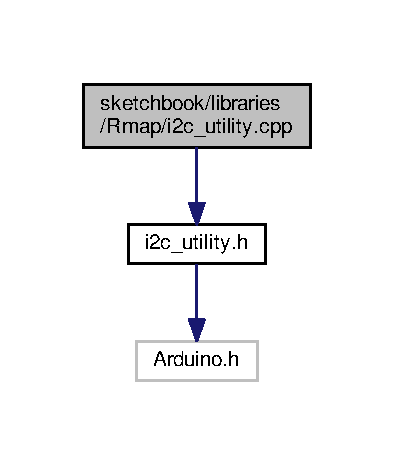
\includegraphics[width=189pt]{i2c__utility_8cpp__incl}
\end{center}
\end{figure}
\subsection*{Functions}
\begin{DoxyCompactItemize}
\item 
uint8\+\_\+t \hyperlink{i2c__utility_8cpp_aa7bc76353bcfeb7f24ffe98e8bf3d69a}{I2\+C\+\_\+\+Clear\+Bus} ()
\end{DoxyCompactItemize}


\subsection{Function Documentation}
\mbox{\Hypertarget{i2c__utility_8cpp_aa7bc76353bcfeb7f24ffe98e8bf3d69a}\label{i2c__utility_8cpp_aa7bc76353bcfeb7f24ffe98e8bf3d69a}} 
\index{i2c\+\_\+utility.\+cpp@{i2c\+\_\+utility.\+cpp}!I2\+C\+\_\+\+Clear\+Bus@{I2\+C\+\_\+\+Clear\+Bus}}
\index{I2\+C\+\_\+\+Clear\+Bus@{I2\+C\+\_\+\+Clear\+Bus}!i2c\+\_\+utility.\+cpp@{i2c\+\_\+utility.\+cpp}}
\subsubsection{\texorpdfstring{I2\+C\+\_\+\+Clear\+Bus()}{I2C\_ClearBus()}}
{\footnotesize\ttfamily uint8\+\_\+t I2\+C\+\_\+\+Clear\+Bus (\begin{DoxyParamCaption}{ }\end{DoxyParamCaption})}

This routine turns off the I2C bus and clears it on return S\+CA and S\+CL pins are tri-\/state inputs. You need to call Wire.\+begin() after this to re-\/enable I2C This routine does N\+OT use the Wire library at all.

returns 0 if bus cleared 1 if S\+CL held low. 2 if S\+DA held low by slave clock stretch for $>$ 2sec 3 if S\+DA held low after 20 clocks. A Repeat Start is a Start occurring after a Start with no intervening Stop. 
\hypertarget{i2c__utility_8h}{}\section{sketchbook/libraries/\+Rmap/i2c\+\_\+utility.h File Reference}
\label{i2c__utility_8h}\index{sketchbook/libraries/\+Rmap/i2c\+\_\+utility.\+h@{sketchbook/libraries/\+Rmap/i2c\+\_\+utility.\+h}}
{\ttfamily \#include $<$Arduino.\+h$>$}\newline
Include dependency graph for i2c\+\_\+utility.\+h\+:\nopagebreak
\begin{figure}[H]
\begin{center}
\leavevmode
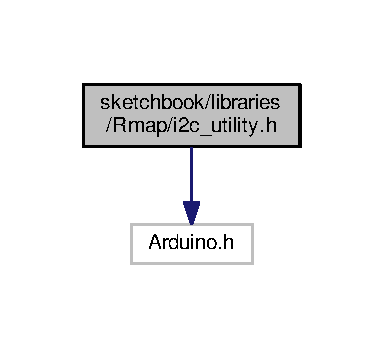
\includegraphics[width=184pt]{i2c__utility_8h__incl}
\end{center}
\end{figure}
This graph shows which files directly or indirectly include this file\+:\nopagebreak
\begin{figure}[H]
\begin{center}
\leavevmode
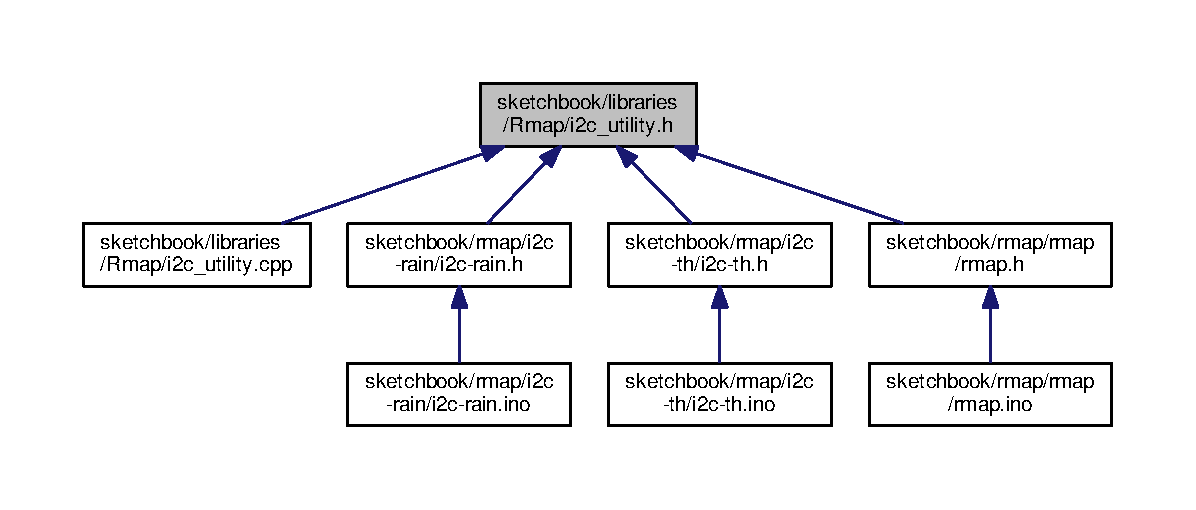
\includegraphics[width=350pt]{i2c__utility_8h__dep__incl}
\end{center}
\end{figure}
\subsection*{Functions}
\begin{DoxyCompactItemize}
\item 
uint8\+\_\+t \hyperlink{i2c__utility_8h_aa7bc76353bcfeb7f24ffe98e8bf3d69a}{I2\+C\+\_\+\+Clear\+Bus} ()
\end{DoxyCompactItemize}


\subsection{Function Documentation}
\mbox{\Hypertarget{i2c__utility_8h_aa7bc76353bcfeb7f24ffe98e8bf3d69a}\label{i2c__utility_8h_aa7bc76353bcfeb7f24ffe98e8bf3d69a}} 
\index{i2c\+\_\+utility.\+h@{i2c\+\_\+utility.\+h}!I2\+C\+\_\+\+Clear\+Bus@{I2\+C\+\_\+\+Clear\+Bus}}
\index{I2\+C\+\_\+\+Clear\+Bus@{I2\+C\+\_\+\+Clear\+Bus}!i2c\+\_\+utility.\+h@{i2c\+\_\+utility.\+h}}
\subsubsection{\texorpdfstring{I2\+C\+\_\+\+Clear\+Bus()}{I2C\_ClearBus()}}
{\footnotesize\ttfamily uint8\+\_\+t I2\+C\+\_\+\+Clear\+Bus (\begin{DoxyParamCaption}{ }\end{DoxyParamCaption})}

This routine turns off the I2C bus and clears it on return S\+CA and S\+CL pins are tri-\/state inputs. You need to call Wire.\+begin() after this to re-\/enable I2C This routine does N\+OT use the Wire library at all.

returns 0 if bus cleared 1 if S\+CL held low. 2 if S\+DA held low by slave clock stretch for $>$ 2sec 3 if S\+DA held low after 20 clocks. A Repeat Start is a Start occurring after a Start with no intervening Stop. 
\hypertarget{registers-rain_8h}{}\section{sketchbook/libraries/\+Rmap/registers-\/rain.h File Reference}
\label{registers-rain_8h}\index{sketchbook/libraries/\+Rmap/registers-\/rain.\+h@{sketchbook/libraries/\+Rmap/registers-\/rain.\+h}}
{\ttfamily \#include \char`\"{}registers.\+h\char`\"{}}\newline
Include dependency graph for registers-\/rain.h\+:\nopagebreak
\begin{figure}[H]
\begin{center}
\leavevmode
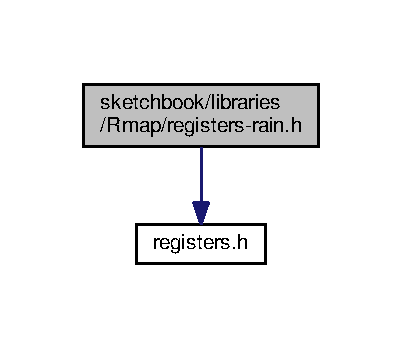
\includegraphics[width=193pt]{registers-rain_8h__incl}
\end{center}
\end{figure}
This graph shows which files directly or indirectly include this file\+:\nopagebreak
\begin{figure}[H]
\begin{center}
\leavevmode
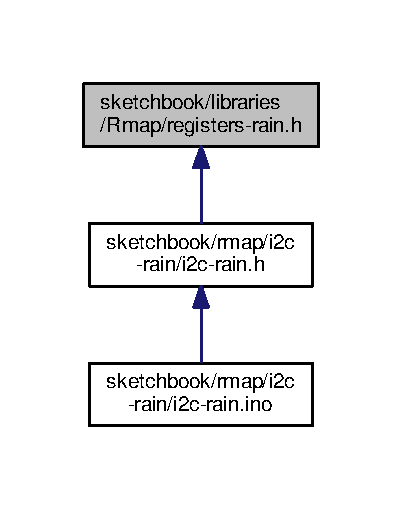
\includegraphics[width=193pt]{registers-rain_8h__dep__incl}
\end{center}
\end{figure}
\subsection*{Macros}
\begin{DoxyCompactItemize}
\item 
\mbox{\Hypertarget{registers-rain_8h_a2aebb0ca4cdf424c57dee6f591c40e0c}\label{registers-rain_8h_a2aebb0ca4cdf424c57dee6f591c40e0c}} 
\#define \hyperlink{registers-rain_8h_a2aebb0ca4cdf424c57dee6f591c40e0c}{I2\+C\+\_\+\+R\+A\+I\+N\+\_\+\+D\+E\+F\+A\+U\+L\+T\+\_\+\+A\+D\+D\+R\+E\+SS}~(0x21)
\begin{DoxyCompactList}\small\item\em Default address for i2c-\/rain module. \end{DoxyCompactList}\item 
\mbox{\Hypertarget{registers-rain_8h_a2317a1a8ab54f27bf55a2ddbbadeff89}\label{registers-rain_8h_a2317a1a8ab54f27bf55a2ddbbadeff89}} 
\#define \hyperlink{registers-rain_8h_a2317a1a8ab54f27bf55a2ddbbadeff89}{I2\+C\+\_\+\+R\+A\+I\+N\+\_\+\+C\+O\+M\+M\+A\+N\+D\+\_\+\+S\+A\+VE}~(0x01)
\begin{DoxyCompactList}\small\item\em Save command for i2c-\/rain module. \end{DoxyCompactList}\item 
\mbox{\Hypertarget{registers-rain_8h_a6893d5ae3ff51fb2c425c0d214a68f23}\label{registers-rain_8h_a6893d5ae3ff51fb2c425c0d214a68f23}} 
\#define \hyperlink{registers-rain_8h_a6893d5ae3ff51fb2c425c0d214a68f23}{I2\+C\+\_\+\+R\+A\+I\+N\+\_\+\+C\+O\+M\+M\+A\+N\+D\+\_\+\+O\+N\+E\+S\+H\+O\+T\+\_\+\+S\+T\+A\+RT}~(0x02)
\begin{DoxyCompactList}\small\item\em Oneshot start command for i2c-\/rain module. \end{DoxyCompactList}\item 
\mbox{\Hypertarget{registers-rain_8h_a0127567ae86a5c8b5fe32c9db08fd5ef}\label{registers-rain_8h_a0127567ae86a5c8b5fe32c9db08fd5ef}} 
\#define \hyperlink{registers-rain_8h_a0127567ae86a5c8b5fe32c9db08fd5ef}{I2\+C\+\_\+\+R\+A\+I\+N\+\_\+\+C\+O\+M\+M\+A\+N\+D\+\_\+\+O\+N\+E\+S\+H\+O\+T\+\_\+\+S\+T\+OP}~(0x03)
\begin{DoxyCompactList}\small\item\em Oneshot stop command for i2c-\/rain module. \end{DoxyCompactList}\item 
\mbox{\Hypertarget{registers-rain_8h_a7e69d765542130687c60f1009e2857ba}\label{registers-rain_8h_a7e69d765542130687c60f1009e2857ba}} 
\#define \hyperlink{registers-rain_8h_a7e69d765542130687c60f1009e2857ba}{I2\+C\+\_\+\+R\+A\+I\+N\+\_\+\+C\+O\+M\+M\+A\+N\+D\+\_\+\+O\+N\+E\+S\+H\+O\+T\+\_\+\+S\+T\+A\+R\+T\+\_\+\+S\+T\+OP}~(0x04)
\begin{DoxyCompactList}\small\item\em Oneshot start-\/stop command for i2c-\/rain module. \end{DoxyCompactList}\item 
\mbox{\Hypertarget{registers-rain_8h_a181a38e0f8a5507ff2b088f9a3c89dc5}\label{registers-rain_8h_a181a38e0f8a5507ff2b088f9a3c89dc5}} 
\#define \hyperlink{registers-rain_8h_a181a38e0f8a5507ff2b088f9a3c89dc5}{I2\+C\+\_\+\+R\+A\+I\+N\+\_\+\+T\+Y\+P\+E\+\_\+\+L\+E\+N\+G\+TH}~(0x01)
\begin{DoxyCompactList}\small\item\em length of the type variable for i2c-\/rain module. \end{DoxyCompactList}\item 
\mbox{\Hypertarget{registers-rain_8h_a3b11f9d8cde7778ef1b91e62b4805704}\label{registers-rain_8h_a3b11f9d8cde7778ef1b91e62b4805704}} 
\#define \hyperlink{registers-rain_8h_a3b11f9d8cde7778ef1b91e62b4805704}{I2\+C\+\_\+\+R\+A\+I\+N\+\_\+\+T\+Y\+P\+E\+\_\+\+A\+D\+D\+R\+E\+SS}~(\hyperlink{registers_8h_ad04d1b7c138bbfcc7672f00defb5f312}{I2\+C\+\_\+\+R\+E\+A\+D\+\_\+\+R\+E\+G\+I\+S\+T\+E\+R\+\_\+\+S\+T\+A\+R\+T\+\_\+\+A\+D\+D\+R\+E\+SS})
\begin{DoxyCompactList}\small\item\em address of the type variable for i2c-\/rain module. \end{DoxyCompactList}\item 
\mbox{\Hypertarget{registers-rain_8h_a61a0b98368463356fd175c65ad070f70}\label{registers-rain_8h_a61a0b98368463356fd175c65ad070f70}} 
\#define \hyperlink{registers-rain_8h_a61a0b98368463356fd175c65ad070f70}{I2\+C\+\_\+\+R\+A\+I\+N\+\_\+\+V\+E\+R\+S\+I\+O\+N\+\_\+\+L\+E\+N\+G\+TH}~(0x01)
\begin{DoxyCompactList}\small\item\em length of the version variable for i2c-\/rain module. \end{DoxyCompactList}\item 
\mbox{\Hypertarget{registers-rain_8h_a9e52019667b12e9673b9d8dcf051ad71}\label{registers-rain_8h_a9e52019667b12e9673b9d8dcf051ad71}} 
\#define \hyperlink{registers-rain_8h_a9e52019667b12e9673b9d8dcf051ad71}{I2\+C\+\_\+\+R\+A\+I\+N\+\_\+\+V\+E\+R\+S\+I\+O\+N\+\_\+\+A\+D\+D\+R\+E\+SS}~(\hyperlink{registers-rain_8h_a3b11f9d8cde7778ef1b91e62b4805704}{I2\+C\+\_\+\+R\+A\+I\+N\+\_\+\+T\+Y\+P\+E\+\_\+\+A\+D\+D\+R\+E\+SS} + \hyperlink{registers-rain_8h_a181a38e0f8a5507ff2b088f9a3c89dc5}{I2\+C\+\_\+\+R\+A\+I\+N\+\_\+\+T\+Y\+P\+E\+\_\+\+L\+E\+N\+G\+TH})
\begin{DoxyCompactList}\small\item\em address of the version variable for i2c-\/rain module. \end{DoxyCompactList}\item 
\mbox{\Hypertarget{registers-rain_8h_a2891a119589f6d2ea69bedc9656dc88d}\label{registers-rain_8h_a2891a119589f6d2ea69bedc9656dc88d}} 
\#define \hyperlink{registers-rain_8h_a2891a119589f6d2ea69bedc9656dc88d}{I2\+C\+\_\+\+R\+A\+I\+N\+\_\+\+T\+I\+P\+S\+\_\+\+L\+E\+N\+G\+TH}~(0x02)
\begin{DoxyCompactList}\small\item\em length of the rain tips variable for i2c-\/rain module. \end{DoxyCompactList}\item 
\mbox{\Hypertarget{registers-rain_8h_a338954266104a386be7cdb52adee3018}\label{registers-rain_8h_a338954266104a386be7cdb52adee3018}} 
\#define \hyperlink{registers-rain_8h_a338954266104a386be7cdb52adee3018}{I2\+C\+\_\+\+R\+A\+I\+N\+\_\+\+T\+I\+P\+S\+\_\+\+A\+D\+D\+R\+E\+SS}~(\hyperlink{registers-rain_8h_a9e52019667b12e9673b9d8dcf051ad71}{I2\+C\+\_\+\+R\+A\+I\+N\+\_\+\+V\+E\+R\+S\+I\+O\+N\+\_\+\+A\+D\+D\+R\+E\+SS} + \hyperlink{registers-rain_8h_a61a0b98368463356fd175c65ad070f70}{I2\+C\+\_\+\+R\+A\+I\+N\+\_\+\+V\+E\+R\+S\+I\+O\+N\+\_\+\+L\+E\+N\+G\+TH})
\begin{DoxyCompactList}\small\item\em address of the rain tips variable for i2c-\/rain module. \end{DoxyCompactList}\item 
\mbox{\Hypertarget{registers-rain_8h_a54d09c3f3315e399f6cd7eb9c1ada389}\label{registers-rain_8h_a54d09c3f3315e399f6cd7eb9c1ada389}} 
\#define \hyperlink{registers-rain_8h_a54d09c3f3315e399f6cd7eb9c1ada389}{I2\+C\+\_\+\+R\+A\+I\+N\+\_\+\+R\+E\+A\+D\+A\+B\+L\+E\+\_\+\+D\+A\+T\+A\+\_\+\+L\+E\+N\+G\+TH}~(\hyperlink{registers-rain_8h_a338954266104a386be7cdb52adee3018}{I2\+C\+\_\+\+R\+A\+I\+N\+\_\+\+T\+I\+P\+S\+\_\+\+A\+D\+D\+R\+E\+SS} + \hyperlink{registers-rain_8h_a2891a119589f6d2ea69bedc9656dc88d}{I2\+C\+\_\+\+R\+A\+I\+N\+\_\+\+T\+I\+P\+S\+\_\+\+L\+E\+N\+G\+TH} -\/ \hyperlink{registers_8h_ad04d1b7c138bbfcc7672f00defb5f312}{I2\+C\+\_\+\+R\+E\+A\+D\+\_\+\+R\+E\+G\+I\+S\+T\+E\+R\+\_\+\+S\+T\+A\+R\+T\+\_\+\+A\+D\+D\+R\+E\+SS})
\begin{DoxyCompactList}\small\item\em length of the readable variables for i2c-\/rain module. Need to be update with with last 2 define!!! \end{DoxyCompactList}\item 
\mbox{\Hypertarget{registers-rain_8h_a71aabb131056ec935e30daee63068ca1}\label{registers-rain_8h_a71aabb131056ec935e30daee63068ca1}} 
\#define \hyperlink{registers-rain_8h_a71aabb131056ec935e30daee63068ca1}{I2\+C\+\_\+\+R\+A\+I\+N\+\_\+\+A\+D\+D\+R\+E\+S\+S\+\_\+\+L\+E\+N\+G\+TH}~(0x01)
\begin{DoxyCompactList}\small\item\em length of the address variable for i2c-\/rain module. \end{DoxyCompactList}\item 
\mbox{\Hypertarget{registers-rain_8h_a80ceb2e20b5e46f7be4fe67afa070962}\label{registers-rain_8h_a80ceb2e20b5e46f7be4fe67afa070962}} 
\#define \hyperlink{registers-rain_8h_a80ceb2e20b5e46f7be4fe67afa070962}{I2\+C\+\_\+\+R\+A\+I\+N\+\_\+\+A\+D\+D\+R\+E\+S\+S\+\_\+\+A\+D\+D\+R\+E\+SS}~(\hyperlink{registers_8h_ad980dee82f83659f0a84e3e1f3c177bb}{I2\+C\+\_\+\+W\+R\+I\+T\+E\+\_\+\+R\+E\+G\+I\+S\+T\+E\+R\+\_\+\+S\+T\+A\+R\+T\+\_\+\+A\+D\+D\+R\+E\+SS})
\begin{DoxyCompactList}\small\item\em address of the address variable for i2c-\/rain module. \end{DoxyCompactList}\item 
\mbox{\Hypertarget{registers-rain_8h_ad238c864994f79289ba720ca751b8f7d}\label{registers-rain_8h_ad238c864994f79289ba720ca751b8f7d}} 
\#define \hyperlink{registers-rain_8h_ad238c864994f79289ba720ca751b8f7d}{I2\+C\+\_\+\+R\+A\+I\+N\+\_\+\+O\+N\+E\+S\+H\+O\+T\+\_\+\+L\+E\+N\+G\+TH}~(0x01)
\begin{DoxyCompactList}\small\item\em length of the oneshot variable for i2c-\/rain module. \end{DoxyCompactList}\item 
\mbox{\Hypertarget{registers-rain_8h_a6fbaaf0f0fcf13291d7a0699ab260d94}\label{registers-rain_8h_a6fbaaf0f0fcf13291d7a0699ab260d94}} 
\#define \hyperlink{registers-rain_8h_a6fbaaf0f0fcf13291d7a0699ab260d94}{I2\+C\+\_\+\+R\+A\+I\+N\+\_\+\+O\+N\+E\+S\+H\+O\+T\+\_\+\+A\+D\+D\+R\+E\+SS}~(\hyperlink{registers-rain_8h_a80ceb2e20b5e46f7be4fe67afa070962}{I2\+C\+\_\+\+R\+A\+I\+N\+\_\+\+A\+D\+D\+R\+E\+S\+S\+\_\+\+A\+D\+D\+R\+E\+SS} + \hyperlink{registers-rain_8h_a71aabb131056ec935e30daee63068ca1}{I2\+C\+\_\+\+R\+A\+I\+N\+\_\+\+A\+D\+D\+R\+E\+S\+S\+\_\+\+L\+E\+N\+G\+TH})
\begin{DoxyCompactList}\small\item\em address of the oneshot variable for i2c-\/rain module. \end{DoxyCompactList}\item 
\mbox{\Hypertarget{registers-rain_8h_af592a5990a1a7566488db79011795cef}\label{registers-rain_8h_af592a5990a1a7566488db79011795cef}} 
\#define \hyperlink{registers-rain_8h_af592a5990a1a7566488db79011795cef}{I2\+C\+\_\+\+R\+A\+I\+N\+\_\+\+C\+O\+N\+T\+I\+N\+U\+O\+U\+S\+\_\+\+L\+E\+N\+G\+TH}~(0x01)
\begin{DoxyCompactList}\small\item\em length of the continuous variable for i2c-\/rain module. \end{DoxyCompactList}\item 
\mbox{\Hypertarget{registers-rain_8h_a75ad23be11d22ec4f3b3d69fcdbf0a64}\label{registers-rain_8h_a75ad23be11d22ec4f3b3d69fcdbf0a64}} 
\#define \hyperlink{registers-rain_8h_a75ad23be11d22ec4f3b3d69fcdbf0a64}{I2\+C\+\_\+\+R\+A\+I\+N\+\_\+\+C\+O\+N\+T\+I\+N\+U\+O\+U\+S\+\_\+\+A\+D\+D\+R\+E\+SS}~(\hyperlink{registers-rain_8h_a6fbaaf0f0fcf13291d7a0699ab260d94}{I2\+C\+\_\+\+R\+A\+I\+N\+\_\+\+O\+N\+E\+S\+H\+O\+T\+\_\+\+A\+D\+D\+R\+E\+SS} + \hyperlink{registers-rain_8h_ad238c864994f79289ba720ca751b8f7d}{I2\+C\+\_\+\+R\+A\+I\+N\+\_\+\+O\+N\+E\+S\+H\+O\+T\+\_\+\+L\+E\+N\+G\+TH})
\begin{DoxyCompactList}\small\item\em address of the continuous variable for i2c-\/rain module. \end{DoxyCompactList}\item 
\mbox{\Hypertarget{registers-rain_8h_ab18763172e0c3d07bce932542f3e6044}\label{registers-rain_8h_ab18763172e0c3d07bce932542f3e6044}} 
\#define \hyperlink{registers-rain_8h_ab18763172e0c3d07bce932542f3e6044}{I2\+C\+\_\+\+R\+A\+I\+N\+\_\+\+W\+R\+I\+T\+A\+B\+L\+E\+\_\+\+D\+A\+T\+A\+\_\+\+L\+E\+N\+G\+TH}~(\hyperlink{registers-rain_8h_a75ad23be11d22ec4f3b3d69fcdbf0a64}{I2\+C\+\_\+\+R\+A\+I\+N\+\_\+\+C\+O\+N\+T\+I\+N\+U\+O\+U\+S\+\_\+\+A\+D\+D\+R\+E\+SS} + \hyperlink{registers-rain_8h_af592a5990a1a7566488db79011795cef}{I2\+C\+\_\+\+R\+A\+I\+N\+\_\+\+C\+O\+N\+T\+I\+N\+U\+O\+U\+S\+\_\+\+L\+E\+N\+G\+TH} -\/ \hyperlink{registers_8h_ad980dee82f83659f0a84e3e1f3c177bb}{I2\+C\+\_\+\+W\+R\+I\+T\+E\+\_\+\+R\+E\+G\+I\+S\+T\+E\+R\+\_\+\+S\+T\+A\+R\+T\+\_\+\+A\+D\+D\+R\+E\+SS})
\begin{DoxyCompactList}\small\item\em length of the writable variables for i2c-\/rain module. \end{DoxyCompactList}\end{DoxyCompactItemize}

\hypertarget{registers-th_8h}{}\section{sketchbook/libraries/\+Rmap/registers-\/th.h File Reference}
\label{registers-th_8h}\index{sketchbook/libraries/\+Rmap/registers-\/th.\+h@{sketchbook/libraries/\+Rmap/registers-\/th.\+h}}
{\ttfamily \#include \char`\"{}registers.\+h\char`\"{}}\newline
Include dependency graph for registers-\/th.h\+:\nopagebreak
\begin{figure}[H]
\begin{center}
\leavevmode
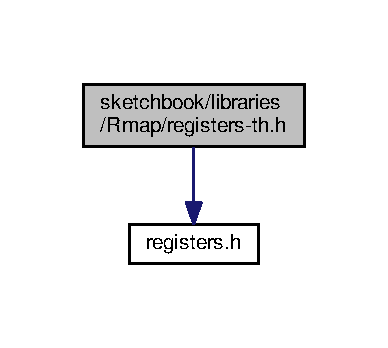
\includegraphics[width=186pt]{registers-th_8h__incl}
\end{center}
\end{figure}
This graph shows which files directly or indirectly include this file\+:\nopagebreak
\begin{figure}[H]
\begin{center}
\leavevmode
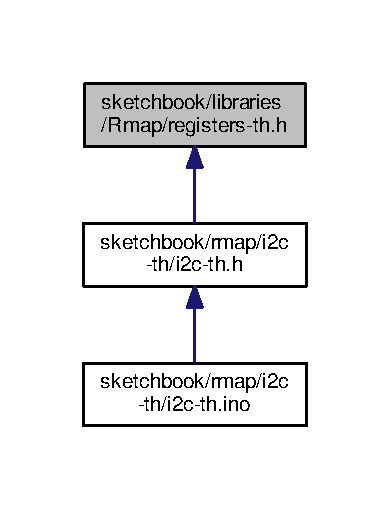
\includegraphics[width=187pt]{registers-th_8h__dep__incl}
\end{center}
\end{figure}
\subsection*{Macros}
\begin{DoxyCompactItemize}
\item 
\mbox{\Hypertarget{registers-th_8h_a66906eb81e92beab5f2076ac49996132}\label{registers-th_8h_a66906eb81e92beab5f2076ac49996132}} 
\#define \hyperlink{registers-th_8h_a66906eb81e92beab5f2076ac49996132}{I2\+C\+\_\+\+T\+H\+\_\+\+D\+E\+F\+A\+U\+L\+T\+\_\+\+A\+D\+D\+R\+E\+SS}~(0x23)
\begin{DoxyCompactList}\small\item\em Default address for i2c-\/th module. \end{DoxyCompactList}\item 
\mbox{\Hypertarget{registers-th_8h_a6d2d1a9b4ae7894be4b062205255f1ff}\label{registers-th_8h_a6d2d1a9b4ae7894be4b062205255f1ff}} 
\#define \hyperlink{registers-th_8h_a6d2d1a9b4ae7894be4b062205255f1ff}{I2\+C\+\_\+\+T\+H\+\_\+\+T\+E\+M\+P\+E\+R\+A\+T\+U\+R\+E\+\_\+\+D\+E\+F\+A\+U\+L\+T\+\_\+\+A\+D\+D\+R\+E\+SS}~(0x49)
\begin{DoxyCompactList}\small\item\em Default address for temperature sensor for i2c-\/th module. \end{DoxyCompactList}\item 
\mbox{\Hypertarget{registers-th_8h_aa7b1a0982e4333dd39c7829eda6baa42}\label{registers-th_8h_aa7b1a0982e4333dd39c7829eda6baa42}} 
\#define \hyperlink{registers-th_8h_aa7b1a0982e4333dd39c7829eda6baa42}{I2\+C\+\_\+\+T\+H\+\_\+\+H\+U\+M\+I\+D\+I\+T\+Y\+\_\+\+D\+E\+F\+A\+U\+L\+T\+\_\+\+A\+D\+D\+R\+E\+SS}~(0x27)
\begin{DoxyCompactList}\small\item\em Default address for humidity sensor for i2c-\/th module. \end{DoxyCompactList}\item 
\mbox{\Hypertarget{registers-th_8h_afafbe31a0d6c332cd66e8a363b332daf}\label{registers-th_8h_afafbe31a0d6c332cd66e8a363b332daf}} 
\#define \hyperlink{registers-th_8h_afafbe31a0d6c332cd66e8a363b332daf}{I2\+C\+\_\+\+T\+H\+\_\+\+C\+O\+M\+M\+A\+N\+D\+\_\+\+S\+A\+VE}~(0x01)
\begin{DoxyCompactList}\small\item\em Save command for i2c-\/th module. \end{DoxyCompactList}\item 
\mbox{\Hypertarget{registers-th_8h_a01ff8debbe24e2777d4669a05bba9aff}\label{registers-th_8h_a01ff8debbe24e2777d4669a05bba9aff}} 
\#define \hyperlink{registers-th_8h_a01ff8debbe24e2777d4669a05bba9aff}{I2\+C\+\_\+\+T\+H\+\_\+\+C\+O\+M\+M\+A\+N\+D\+\_\+\+O\+N\+E\+S\+H\+O\+T\+\_\+\+S\+T\+A\+RT}~(0x02)
\begin{DoxyCompactList}\small\item\em Oneshot start command for i2c-\/th module. \end{DoxyCompactList}\item 
\mbox{\Hypertarget{registers-th_8h_a75c843dd544aae25cc6328327d357b90}\label{registers-th_8h_a75c843dd544aae25cc6328327d357b90}} 
\#define \hyperlink{registers-th_8h_a75c843dd544aae25cc6328327d357b90}{I2\+C\+\_\+\+T\+H\+\_\+\+C\+O\+M\+M\+A\+N\+D\+\_\+\+O\+N\+E\+S\+H\+O\+T\+\_\+\+S\+T\+OP}~(0x03)
\begin{DoxyCompactList}\small\item\em Oneshot stop command for i2c-\/th module. \end{DoxyCompactList}\item 
\mbox{\Hypertarget{registers-th_8h_af5fa530b0e40a9903afdf3a1c646b4d7}\label{registers-th_8h_af5fa530b0e40a9903afdf3a1c646b4d7}} 
\#define \hyperlink{registers-th_8h_af5fa530b0e40a9903afdf3a1c646b4d7}{I2\+C\+\_\+\+T\+H\+\_\+\+C\+O\+M\+M\+A\+N\+D\+\_\+\+O\+N\+E\+S\+H\+O\+T\+\_\+\+S\+T\+A\+R\+T\+\_\+\+S\+T\+OP}~(0x04)
\begin{DoxyCompactList}\small\item\em Oneshot start-\/stop command for i2c-\/th module. \end{DoxyCompactList}\item 
\mbox{\Hypertarget{registers-th_8h_a51680f0c924ae23831dbd2a099f0e92f}\label{registers-th_8h_a51680f0c924ae23831dbd2a099f0e92f}} 
\#define \hyperlink{registers-th_8h_a51680f0c924ae23831dbd2a099f0e92f}{I2\+C\+\_\+\+T\+H\+\_\+\+C\+O\+M\+M\+A\+N\+D\+\_\+\+C\+O\+N\+T\+I\+N\+U\+O\+U\+S\+\_\+\+S\+T\+A\+RT}~(0x05)
\begin{DoxyCompactList}\small\item\em Continuous start command for i2c-\/th module. \end{DoxyCompactList}\item 
\mbox{\Hypertarget{registers-th_8h_ae7a198cd962e2d0099c464eab6aae1d3}\label{registers-th_8h_ae7a198cd962e2d0099c464eab6aae1d3}} 
\#define \hyperlink{registers-th_8h_ae7a198cd962e2d0099c464eab6aae1d3}{I2\+C\+\_\+\+T\+H\+\_\+\+C\+O\+M\+M\+A\+N\+D\+\_\+\+C\+O\+N\+T\+I\+N\+U\+O\+U\+S\+\_\+\+S\+T\+OP}~(0x06)
\begin{DoxyCompactList}\small\item\em Continuous stop command for i2c-\/th module. \end{DoxyCompactList}\item 
\mbox{\Hypertarget{registers-th_8h_a21a1375a228e3e8aa42a0d5a63b0525d}\label{registers-th_8h_a21a1375a228e3e8aa42a0d5a63b0525d}} 
\#define \hyperlink{registers-th_8h_a21a1375a228e3e8aa42a0d5a63b0525d}{I2\+C\+\_\+\+T\+H\+\_\+\+C\+O\+M\+M\+A\+N\+D\+\_\+\+C\+O\+N\+T\+I\+N\+U\+O\+U\+S\+\_\+\+S\+T\+A\+R\+T\+\_\+\+S\+T\+OP}~(0x07)
\begin{DoxyCompactList}\small\item\em Continuous start-\/stop command for i2c-\/th module. \end{DoxyCompactList}\item 
\mbox{\Hypertarget{registers-th_8h_a0cbb42c5d740febc30ebacafc0fe92f9}\label{registers-th_8h_a0cbb42c5d740febc30ebacafc0fe92f9}} 
\#define \hyperlink{registers-th_8h_a0cbb42c5d740febc30ebacafc0fe92f9}{I2\+C\+\_\+\+T\+H\+\_\+\+T\+Y\+P\+E\+\_\+\+L\+E\+N\+G\+TH}~(0x01)
\begin{DoxyCompactList}\small\item\em length of the type variable for i2c-\/th module. \end{DoxyCompactList}\item 
\mbox{\Hypertarget{registers-th_8h_ae0b56541b450305c37323bfb723be2f7}\label{registers-th_8h_ae0b56541b450305c37323bfb723be2f7}} 
\#define \hyperlink{registers-th_8h_ae0b56541b450305c37323bfb723be2f7}{I2\+C\+\_\+\+T\+H\+\_\+\+T\+Y\+P\+E\+\_\+\+A\+D\+D\+R\+E\+SS}~(\hyperlink{registers_8h_ad04d1b7c138bbfcc7672f00defb5f312}{I2\+C\+\_\+\+R\+E\+A\+D\+\_\+\+R\+E\+G\+I\+S\+T\+E\+R\+\_\+\+S\+T\+A\+R\+T\+\_\+\+A\+D\+D\+R\+E\+SS})
\begin{DoxyCompactList}\small\item\em address of the type variable for i2c-\/th module. \end{DoxyCompactList}\item 
\mbox{\Hypertarget{registers-th_8h_ae5c39794517db2f849788f74d0f5d71a}\label{registers-th_8h_ae5c39794517db2f849788f74d0f5d71a}} 
\#define \hyperlink{registers-th_8h_ae5c39794517db2f849788f74d0f5d71a}{I2\+C\+\_\+\+T\+H\+\_\+\+V\+E\+R\+S\+I\+O\+N\+\_\+\+L\+E\+N\+G\+TH}~(0x01)
\begin{DoxyCompactList}\small\item\em length of the version variable for i2c-\/th module. \end{DoxyCompactList}\item 
\mbox{\Hypertarget{registers-th_8h_a264c5b05353c735ad1d5d91550b12cc7}\label{registers-th_8h_a264c5b05353c735ad1d5d91550b12cc7}} 
\#define \hyperlink{registers-th_8h_a264c5b05353c735ad1d5d91550b12cc7}{I2\+C\+\_\+\+T\+H\+\_\+\+V\+E\+R\+S\+I\+O\+N\+\_\+\+A\+D\+D\+R\+E\+SS}~(\hyperlink{registers-th_8h_ae0b56541b450305c37323bfb723be2f7}{I2\+C\+\_\+\+T\+H\+\_\+\+T\+Y\+P\+E\+\_\+\+A\+D\+D\+R\+E\+SS} + \hyperlink{registers-th_8h_a0cbb42c5d740febc30ebacafc0fe92f9}{I2\+C\+\_\+\+T\+H\+\_\+\+T\+Y\+P\+E\+\_\+\+L\+E\+N\+G\+TH})
\begin{DoxyCompactList}\small\item\em address of the version variable for i2c-\/th module. \end{DoxyCompactList}\item 
\mbox{\Hypertarget{registers-th_8h_a68ba9de54f0dafd98abd7c087aea042f}\label{registers-th_8h_a68ba9de54f0dafd98abd7c087aea042f}} 
\#define \hyperlink{registers-th_8h_a68ba9de54f0dafd98abd7c087aea042f}{I2\+C\+\_\+\+T\+H\+\_\+\+T\+E\+M\+P\+E\+R\+A\+T\+U\+R\+E\+\_\+\+S\+A\+M\+P\+L\+E\+\_\+\+L\+E\+N\+G\+TH}~(0x02)
\begin{DoxyCompactList}\small\item\em length of the temperature sample variable for i2c-\/th module. \end{DoxyCompactList}\item 
\mbox{\Hypertarget{registers-th_8h_a44805161261d958e1e20df79568953cc}\label{registers-th_8h_a44805161261d958e1e20df79568953cc}} 
\#define \hyperlink{registers-th_8h_a44805161261d958e1e20df79568953cc}{I2\+C\+\_\+\+T\+H\+\_\+\+T\+E\+M\+P\+E\+R\+A\+T\+U\+R\+E\+\_\+\+S\+A\+M\+P\+L\+E\+\_\+\+A\+D\+D\+R\+E\+SS}~(\hyperlink{registers-th_8h_a264c5b05353c735ad1d5d91550b12cc7}{I2\+C\+\_\+\+T\+H\+\_\+\+V\+E\+R\+S\+I\+O\+N\+\_\+\+A\+D\+D\+R\+E\+SS} + \hyperlink{registers-th_8h_ae5c39794517db2f849788f74d0f5d71a}{I2\+C\+\_\+\+T\+H\+\_\+\+V\+E\+R\+S\+I\+O\+N\+\_\+\+L\+E\+N\+G\+TH})
\begin{DoxyCompactList}\small\item\em address of the temperature sample variable for i2c-\/th module. \end{DoxyCompactList}\item 
\mbox{\Hypertarget{registers-th_8h_ac6f3b8ab3eade373310b50c2248bac95}\label{registers-th_8h_ac6f3b8ab3eade373310b50c2248bac95}} 
\#define \hyperlink{registers-th_8h_ac6f3b8ab3eade373310b50c2248bac95}{I2\+C\+\_\+\+T\+H\+\_\+\+T\+E\+M\+P\+E\+R\+A\+T\+U\+R\+E\+\_\+\+M\+E\+D60\+\_\+\+L\+E\+N\+G\+TH}~(0x02)
\begin{DoxyCompactList}\small\item\em length of the temperature observation variable for i2c-\/th module. \end{DoxyCompactList}\item 
\mbox{\Hypertarget{registers-th_8h_a0defa72b89f6bbfe41feb464a1eb6c81}\label{registers-th_8h_a0defa72b89f6bbfe41feb464a1eb6c81}} 
\#define \hyperlink{registers-th_8h_a0defa72b89f6bbfe41feb464a1eb6c81}{I2\+C\+\_\+\+T\+H\+\_\+\+T\+E\+M\+P\+E\+R\+A\+T\+U\+R\+E\+\_\+\+M\+E\+D60\+\_\+\+A\+D\+D\+R\+E\+SS}~(\hyperlink{registers-th_8h_a44805161261d958e1e20df79568953cc}{I2\+C\+\_\+\+T\+H\+\_\+\+T\+E\+M\+P\+E\+R\+A\+T\+U\+R\+E\+\_\+\+S\+A\+M\+P\+L\+E\+\_\+\+A\+D\+D\+R\+E\+SS} + \hyperlink{registers-th_8h_a68ba9de54f0dafd98abd7c087aea042f}{I2\+C\+\_\+\+T\+H\+\_\+\+T\+E\+M\+P\+E\+R\+A\+T\+U\+R\+E\+\_\+\+S\+A\+M\+P\+L\+E\+\_\+\+L\+E\+N\+G\+TH})
\begin{DoxyCompactList}\small\item\em address of the temperature observation variable for i2c-\/th module. \end{DoxyCompactList}\item 
\mbox{\Hypertarget{registers-th_8h_ae58cfee6bace2cb489b10eb56a4ce7e4}\label{registers-th_8h_ae58cfee6bace2cb489b10eb56a4ce7e4}} 
\#define \hyperlink{registers-th_8h_ae58cfee6bace2cb489b10eb56a4ce7e4}{I2\+C\+\_\+\+T\+H\+\_\+\+T\+E\+M\+P\+E\+R\+A\+T\+U\+R\+E\+\_\+\+M\+E\+D\+\_\+\+L\+E\+N\+G\+TH}~(0x02)
\begin{DoxyCompactList}\small\item\em length of the average temperature variable for i2c-\/th module. \end{DoxyCompactList}\item 
\mbox{\Hypertarget{registers-th_8h_a805a88b64e74c7a02286550560457b1d}\label{registers-th_8h_a805a88b64e74c7a02286550560457b1d}} 
\#define \hyperlink{registers-th_8h_a805a88b64e74c7a02286550560457b1d}{I2\+C\+\_\+\+T\+H\+\_\+\+T\+E\+M\+P\+E\+R\+A\+T\+U\+R\+E\+\_\+\+M\+E\+D\+\_\+\+A\+D\+D\+R\+E\+SS}~(\hyperlink{registers-th_8h_a0defa72b89f6bbfe41feb464a1eb6c81}{I2\+C\+\_\+\+T\+H\+\_\+\+T\+E\+M\+P\+E\+R\+A\+T\+U\+R\+E\+\_\+\+M\+E\+D60\+\_\+\+A\+D\+D\+R\+E\+SS} + \hyperlink{registers-th_8h_ac6f3b8ab3eade373310b50c2248bac95}{I2\+C\+\_\+\+T\+H\+\_\+\+T\+E\+M\+P\+E\+R\+A\+T\+U\+R\+E\+\_\+\+M\+E\+D60\+\_\+\+L\+E\+N\+G\+TH})
\begin{DoxyCompactList}\small\item\em address of the average temperature variable for i2c-\/th module. \end{DoxyCompactList}\item 
\mbox{\Hypertarget{registers-th_8h_a919ba5b2f1aea01d8b48ac119d705552}\label{registers-th_8h_a919ba5b2f1aea01d8b48ac119d705552}} 
\#define \hyperlink{registers-th_8h_a919ba5b2f1aea01d8b48ac119d705552}{I2\+C\+\_\+\+T\+H\+\_\+\+T\+E\+M\+P\+E\+R\+A\+T\+U\+R\+E\+\_\+\+M\+A\+X\+\_\+\+L\+E\+N\+G\+TH}~(0x02)
\begin{DoxyCompactList}\small\item\em length of the maximum temperature variable for i2c-\/th module. \end{DoxyCompactList}\item 
\mbox{\Hypertarget{registers-th_8h_a6d5b14a0e8a228589bdb9ece79d757fd}\label{registers-th_8h_a6d5b14a0e8a228589bdb9ece79d757fd}} 
\#define \hyperlink{registers-th_8h_a6d5b14a0e8a228589bdb9ece79d757fd}{I2\+C\+\_\+\+T\+H\+\_\+\+T\+E\+M\+P\+E\+R\+A\+T\+U\+R\+E\+\_\+\+M\+A\+X\+\_\+\+A\+D\+D\+R\+E\+SS}~(\hyperlink{registers-th_8h_a805a88b64e74c7a02286550560457b1d}{I2\+C\+\_\+\+T\+H\+\_\+\+T\+E\+M\+P\+E\+R\+A\+T\+U\+R\+E\+\_\+\+M\+E\+D\+\_\+\+A\+D\+D\+R\+E\+SS} + \hyperlink{registers-th_8h_ae58cfee6bace2cb489b10eb56a4ce7e4}{I2\+C\+\_\+\+T\+H\+\_\+\+T\+E\+M\+P\+E\+R\+A\+T\+U\+R\+E\+\_\+\+M\+E\+D\+\_\+\+L\+E\+N\+G\+TH})
\begin{DoxyCompactList}\small\item\em address of the maximum temperature variable for i2c-\/th module. \end{DoxyCompactList}\item 
\mbox{\Hypertarget{registers-th_8h_a6d360f6fa8df3c5d6f52758de9a24c11}\label{registers-th_8h_a6d360f6fa8df3c5d6f52758de9a24c11}} 
\#define \hyperlink{registers-th_8h_a6d360f6fa8df3c5d6f52758de9a24c11}{I2\+C\+\_\+\+T\+H\+\_\+\+T\+E\+M\+P\+E\+R\+A\+T\+U\+R\+E\+\_\+\+M\+I\+N\+\_\+\+L\+E\+N\+G\+TH}~(0x02)
\begin{DoxyCompactList}\small\item\em length of the minimum temperature variable for i2c-\/th module. \end{DoxyCompactList}\item 
\mbox{\Hypertarget{registers-th_8h_a7481bfd98d8da5c9977dfd2f06fc963c}\label{registers-th_8h_a7481bfd98d8da5c9977dfd2f06fc963c}} 
\#define \hyperlink{registers-th_8h_a7481bfd98d8da5c9977dfd2f06fc963c}{I2\+C\+\_\+\+T\+H\+\_\+\+T\+E\+M\+P\+E\+R\+A\+T\+U\+R\+E\+\_\+\+M\+I\+N\+\_\+\+A\+D\+D\+R\+E\+SS}~(\hyperlink{registers-th_8h_a6d5b14a0e8a228589bdb9ece79d757fd}{I2\+C\+\_\+\+T\+H\+\_\+\+T\+E\+M\+P\+E\+R\+A\+T\+U\+R\+E\+\_\+\+M\+A\+X\+\_\+\+A\+D\+D\+R\+E\+SS} + \hyperlink{registers-th_8h_a919ba5b2f1aea01d8b48ac119d705552}{I2\+C\+\_\+\+T\+H\+\_\+\+T\+E\+M\+P\+E\+R\+A\+T\+U\+R\+E\+\_\+\+M\+A\+X\+\_\+\+L\+E\+N\+G\+TH})
\begin{DoxyCompactList}\small\item\em address of the minimum temperature variable for i2c-\/th module. \end{DoxyCompactList}\item 
\mbox{\Hypertarget{registers-th_8h_adb95f4cc071476c164346dc15de2dd1a}\label{registers-th_8h_adb95f4cc071476c164346dc15de2dd1a}} 
\#define \hyperlink{registers-th_8h_adb95f4cc071476c164346dc15de2dd1a}{I2\+C\+\_\+\+T\+H\+\_\+\+T\+E\+M\+P\+E\+R\+A\+T\+U\+R\+E\+\_\+\+S\+I\+G\+M\+A\+\_\+\+L\+E\+N\+G\+TH}~(0x02)
\begin{DoxyCompactList}\small\item\em length of the sigma temperature variable for i2c-\/th module. \end{DoxyCompactList}\item 
\mbox{\Hypertarget{registers-th_8h_a13174bfc9826a2360b3a9ef42c682415}\label{registers-th_8h_a13174bfc9826a2360b3a9ef42c682415}} 
\#define \hyperlink{registers-th_8h_a13174bfc9826a2360b3a9ef42c682415}{I2\+C\+\_\+\+T\+H\+\_\+\+T\+E\+M\+P\+E\+R\+A\+T\+U\+R\+E\+\_\+\+S\+I\+G\+M\+A\+\_\+\+A\+D\+D\+R\+E\+SS}~(\hyperlink{registers-th_8h_a7481bfd98d8da5c9977dfd2f06fc963c}{I2\+C\+\_\+\+T\+H\+\_\+\+T\+E\+M\+P\+E\+R\+A\+T\+U\+R\+E\+\_\+\+M\+I\+N\+\_\+\+A\+D\+D\+R\+E\+SS} + \hyperlink{registers-th_8h_a6d360f6fa8df3c5d6f52758de9a24c11}{I2\+C\+\_\+\+T\+H\+\_\+\+T\+E\+M\+P\+E\+R\+A\+T\+U\+R\+E\+\_\+\+M\+I\+N\+\_\+\+L\+E\+N\+G\+TH})
\begin{DoxyCompactList}\small\item\em address of the sigma temperature variable for i2c-\/th module. \end{DoxyCompactList}\item 
\mbox{\Hypertarget{registers-th_8h_a142a65f1eb8b87e05640583cf0f9d380}\label{registers-th_8h_a142a65f1eb8b87e05640583cf0f9d380}} 
\#define \hyperlink{registers-th_8h_a142a65f1eb8b87e05640583cf0f9d380}{I2\+C\+\_\+\+T\+H\+\_\+\+T\+E\+M\+P\+E\+R\+A\+T\+U\+R\+E\+\_\+\+D\+A\+T\+A\+\_\+\+M\+A\+X\+\_\+\+L\+E\+N\+G\+TH}~(0x02)
\begin{DoxyCompactList}\small\item\em length of the temperature data variable for i2c-\/th module. \end{DoxyCompactList}\item 
\mbox{\Hypertarget{registers-th_8h_a65dca74d31862278a1846c21d23c844d}\label{registers-th_8h_a65dca74d31862278a1846c21d23c844d}} 
\#define \hyperlink{registers-th_8h_a65dca74d31862278a1846c21d23c844d}{I2\+C\+\_\+\+T\+H\+\_\+\+H\+U\+M\+I\+D\+I\+T\+Y\+\_\+\+S\+A\+M\+P\+L\+E\+\_\+\+L\+E\+N\+G\+TH}~(0x02)
\begin{DoxyCompactList}\small\item\em length of the humidity sample variable for i2c-\/th module. \end{DoxyCompactList}\item 
\mbox{\Hypertarget{registers-th_8h_a82d3a5a7a97efcf0b2aa503c0c6de2a5}\label{registers-th_8h_a82d3a5a7a97efcf0b2aa503c0c6de2a5}} 
\#define \hyperlink{registers-th_8h_a82d3a5a7a97efcf0b2aa503c0c6de2a5}{I2\+C\+\_\+\+T\+H\+\_\+\+H\+U\+M\+I\+D\+I\+T\+Y\+\_\+\+S\+A\+M\+P\+L\+E\+\_\+\+A\+D\+D\+R\+E\+SS}~(\hyperlink{registers-th_8h_a13174bfc9826a2360b3a9ef42c682415}{I2\+C\+\_\+\+T\+H\+\_\+\+T\+E\+M\+P\+E\+R\+A\+T\+U\+R\+E\+\_\+\+S\+I\+G\+M\+A\+\_\+\+A\+D\+D\+R\+E\+SS} + \hyperlink{registers-th_8h_adb95f4cc071476c164346dc15de2dd1a}{I2\+C\+\_\+\+T\+H\+\_\+\+T\+E\+M\+P\+E\+R\+A\+T\+U\+R\+E\+\_\+\+S\+I\+G\+M\+A\+\_\+\+L\+E\+N\+G\+TH})
\begin{DoxyCompactList}\small\item\em address of the humidity sample variable for i2c-\/th module. \end{DoxyCompactList}\item 
\mbox{\Hypertarget{registers-th_8h_a0a468dccdfa6ca2993e960b85661efa5}\label{registers-th_8h_a0a468dccdfa6ca2993e960b85661efa5}} 
\#define \hyperlink{registers-th_8h_a0a468dccdfa6ca2993e960b85661efa5}{I2\+C\+\_\+\+T\+H\+\_\+\+H\+U\+M\+I\+D\+I\+T\+Y\+\_\+\+M\+E\+D60\+\_\+\+L\+E\+N\+G\+TH}~(0x02)
\begin{DoxyCompactList}\small\item\em length of the humidity observation variable for i2c-\/th module. \end{DoxyCompactList}\item 
\mbox{\Hypertarget{registers-th_8h_a394425b89ec96065d52723ec5d9688e0}\label{registers-th_8h_a394425b89ec96065d52723ec5d9688e0}} 
\#define \hyperlink{registers-th_8h_a394425b89ec96065d52723ec5d9688e0}{I2\+C\+\_\+\+T\+H\+\_\+\+H\+U\+M\+I\+D\+I\+T\+Y\+\_\+\+M\+E\+D60\+\_\+\+A\+D\+D\+R\+E\+SS}~(\hyperlink{registers-th_8h_a82d3a5a7a97efcf0b2aa503c0c6de2a5}{I2\+C\+\_\+\+T\+H\+\_\+\+H\+U\+M\+I\+D\+I\+T\+Y\+\_\+\+S\+A\+M\+P\+L\+E\+\_\+\+A\+D\+D\+R\+E\+SS} + \hyperlink{registers-th_8h_a65dca74d31862278a1846c21d23c844d}{I2\+C\+\_\+\+T\+H\+\_\+\+H\+U\+M\+I\+D\+I\+T\+Y\+\_\+\+S\+A\+M\+P\+L\+E\+\_\+\+L\+E\+N\+G\+TH})
\begin{DoxyCompactList}\small\item\em address of the humidity observation variable for i2c-\/th module. \end{DoxyCompactList}\item 
\mbox{\Hypertarget{registers-th_8h_ab8c23d04d8c4c952919ca1c4e414dab6}\label{registers-th_8h_ab8c23d04d8c4c952919ca1c4e414dab6}} 
\#define \hyperlink{registers-th_8h_ab8c23d04d8c4c952919ca1c4e414dab6}{I2\+C\+\_\+\+T\+H\+\_\+\+H\+U\+M\+I\+D\+I\+T\+Y\+\_\+\+M\+E\+D\+\_\+\+L\+E\+N\+G\+TH}~(0x02)
\begin{DoxyCompactList}\small\item\em length of the average humidity variable for i2c-\/th module. \end{DoxyCompactList}\item 
\mbox{\Hypertarget{registers-th_8h_a892db1b7b4d94ccdc702a0ef24df6086}\label{registers-th_8h_a892db1b7b4d94ccdc702a0ef24df6086}} 
\#define \hyperlink{registers-th_8h_a892db1b7b4d94ccdc702a0ef24df6086}{I2\+C\+\_\+\+T\+H\+\_\+\+H\+U\+M\+I\+D\+I\+T\+Y\+\_\+\+M\+E\+D\+\_\+\+A\+D\+D\+R\+E\+SS}~(\hyperlink{registers-th_8h_a394425b89ec96065d52723ec5d9688e0}{I2\+C\+\_\+\+T\+H\+\_\+\+H\+U\+M\+I\+D\+I\+T\+Y\+\_\+\+M\+E\+D60\+\_\+\+A\+D\+D\+R\+E\+SS} + \hyperlink{registers-th_8h_a0a468dccdfa6ca2993e960b85661efa5}{I2\+C\+\_\+\+T\+H\+\_\+\+H\+U\+M\+I\+D\+I\+T\+Y\+\_\+\+M\+E\+D60\+\_\+\+L\+E\+N\+G\+TH})
\begin{DoxyCompactList}\small\item\em address of the average humidity variable for i2c-\/th module. \end{DoxyCompactList}\item 
\mbox{\Hypertarget{registers-th_8h_a382c80f1ba03d2f3bc156499d28de9e5}\label{registers-th_8h_a382c80f1ba03d2f3bc156499d28de9e5}} 
\#define \hyperlink{registers-th_8h_a382c80f1ba03d2f3bc156499d28de9e5}{I2\+C\+\_\+\+T\+H\+\_\+\+H\+U\+M\+I\+D\+I\+T\+Y\+\_\+\+M\+A\+X\+\_\+\+L\+E\+N\+G\+TH}~(0x02)
\begin{DoxyCompactList}\small\item\em length of the maximum humidity variable for i2c-\/th module. \end{DoxyCompactList}\item 
\mbox{\Hypertarget{registers-th_8h_ad2f26a7b53f478e0dae29960152ae095}\label{registers-th_8h_ad2f26a7b53f478e0dae29960152ae095}} 
\#define \hyperlink{registers-th_8h_ad2f26a7b53f478e0dae29960152ae095}{I2\+C\+\_\+\+T\+H\+\_\+\+H\+U\+M\+I\+D\+I\+T\+Y\+\_\+\+M\+A\+X\+\_\+\+A\+D\+D\+R\+E\+SS}~(\hyperlink{registers-th_8h_a892db1b7b4d94ccdc702a0ef24df6086}{I2\+C\+\_\+\+T\+H\+\_\+\+H\+U\+M\+I\+D\+I\+T\+Y\+\_\+\+M\+E\+D\+\_\+\+A\+D\+D\+R\+E\+SS} + \hyperlink{registers-th_8h_ab8c23d04d8c4c952919ca1c4e414dab6}{I2\+C\+\_\+\+T\+H\+\_\+\+H\+U\+M\+I\+D\+I\+T\+Y\+\_\+\+M\+E\+D\+\_\+\+L\+E\+N\+G\+TH})
\begin{DoxyCompactList}\small\item\em address of the maximum humidity variable for i2c-\/th module. \end{DoxyCompactList}\item 
\mbox{\Hypertarget{registers-th_8h_a7f9d59a93a51fa58d1fa0fc389a2ff93}\label{registers-th_8h_a7f9d59a93a51fa58d1fa0fc389a2ff93}} 
\#define \hyperlink{registers-th_8h_a7f9d59a93a51fa58d1fa0fc389a2ff93}{I2\+C\+\_\+\+T\+H\+\_\+\+H\+U\+M\+I\+D\+I\+T\+Y\+\_\+\+M\+I\+N\+\_\+\+L\+E\+N\+G\+TH}~(0x02)
\begin{DoxyCompactList}\small\item\em length of the minimum humidity variable for i2c-\/th module. \end{DoxyCompactList}\item 
\mbox{\Hypertarget{registers-th_8h_a707f2aa68826eec93b19e8426ab86d02}\label{registers-th_8h_a707f2aa68826eec93b19e8426ab86d02}} 
\#define \hyperlink{registers-th_8h_a707f2aa68826eec93b19e8426ab86d02}{I2\+C\+\_\+\+T\+H\+\_\+\+H\+U\+M\+I\+D\+I\+T\+Y\+\_\+\+M\+I\+N\+\_\+\+A\+D\+D\+R\+E\+SS}~(\hyperlink{registers-th_8h_ad2f26a7b53f478e0dae29960152ae095}{I2\+C\+\_\+\+T\+H\+\_\+\+H\+U\+M\+I\+D\+I\+T\+Y\+\_\+\+M\+A\+X\+\_\+\+A\+D\+D\+R\+E\+SS} + \hyperlink{registers-th_8h_a382c80f1ba03d2f3bc156499d28de9e5}{I2\+C\+\_\+\+T\+H\+\_\+\+H\+U\+M\+I\+D\+I\+T\+Y\+\_\+\+M\+A\+X\+\_\+\+L\+E\+N\+G\+TH})
\begin{DoxyCompactList}\small\item\em address of the minimum humidity variable for i2c-\/th module. \end{DoxyCompactList}\item 
\mbox{\Hypertarget{registers-th_8h_ac845881a1c5e3caa152724619e298044}\label{registers-th_8h_ac845881a1c5e3caa152724619e298044}} 
\#define \hyperlink{registers-th_8h_ac845881a1c5e3caa152724619e298044}{I2\+C\+\_\+\+T\+H\+\_\+\+H\+U\+M\+I\+D\+I\+T\+Y\+\_\+\+S\+I\+G\+M\+A\+\_\+\+L\+E\+N\+G\+TH}~(0x02)
\begin{DoxyCompactList}\small\item\em length of the sigma humidity variable for i2c-\/th module. \end{DoxyCompactList}\item 
\mbox{\Hypertarget{registers-th_8h_a79c69759f7f0b6db1938a786d214296f}\label{registers-th_8h_a79c69759f7f0b6db1938a786d214296f}} 
\#define \hyperlink{registers-th_8h_a79c69759f7f0b6db1938a786d214296f}{I2\+C\+\_\+\+T\+H\+\_\+\+H\+U\+M\+I\+D\+I\+T\+Y\+\_\+\+S\+I\+G\+M\+A\+\_\+\+A\+D\+D\+R\+E\+SS}~(\hyperlink{registers-th_8h_a707f2aa68826eec93b19e8426ab86d02}{I2\+C\+\_\+\+T\+H\+\_\+\+H\+U\+M\+I\+D\+I\+T\+Y\+\_\+\+M\+I\+N\+\_\+\+A\+D\+D\+R\+E\+SS} + \hyperlink{registers-th_8h_a7f9d59a93a51fa58d1fa0fc389a2ff93}{I2\+C\+\_\+\+T\+H\+\_\+\+H\+U\+M\+I\+D\+I\+T\+Y\+\_\+\+M\+I\+N\+\_\+\+L\+E\+N\+G\+TH})
\begin{DoxyCompactList}\small\item\em address of the sigma humidity variable for i2c-\/th module. \end{DoxyCompactList}\item 
\mbox{\Hypertarget{registers-th_8h_a0c76a423b5e600174e4b6502f6f19762}\label{registers-th_8h_a0c76a423b5e600174e4b6502f6f19762}} 
\#define \hyperlink{registers-th_8h_a0c76a423b5e600174e4b6502f6f19762}{I2\+C\+\_\+\+T\+H\+\_\+\+H\+U\+M\+I\+D\+I\+T\+Y\+\_\+\+D\+A\+T\+A\+\_\+\+M\+A\+X\+\_\+\+L\+E\+N\+G\+TH}~(0x02)
\begin{DoxyCompactList}\small\item\em length of the humidity data variable for i2c-\/th module. \end{DoxyCompactList}\item 
\mbox{\Hypertarget{registers-th_8h_a1ffb1262654d227edede5e899883291e}\label{registers-th_8h_a1ffb1262654d227edede5e899883291e}} 
\#define \hyperlink{registers-th_8h_a1ffb1262654d227edede5e899883291e}{I2\+C\+\_\+\+T\+H\+\_\+\+R\+E\+A\+D\+A\+B\+L\+E\+\_\+\+D\+A\+T\+A\+\_\+\+L\+E\+N\+G\+TH}~(\hyperlink{registers-th_8h_a79c69759f7f0b6db1938a786d214296f}{I2\+C\+\_\+\+T\+H\+\_\+\+H\+U\+M\+I\+D\+I\+T\+Y\+\_\+\+S\+I\+G\+M\+A\+\_\+\+A\+D\+D\+R\+E\+SS} + \hyperlink{registers-th_8h_ac845881a1c5e3caa152724619e298044}{I2\+C\+\_\+\+T\+H\+\_\+\+H\+U\+M\+I\+D\+I\+T\+Y\+\_\+\+S\+I\+G\+M\+A\+\_\+\+L\+E\+N\+G\+TH} -\/ \hyperlink{registers_8h_ad04d1b7c138bbfcc7672f00defb5f312}{I2\+C\+\_\+\+R\+E\+A\+D\+\_\+\+R\+E\+G\+I\+S\+T\+E\+R\+\_\+\+S\+T\+A\+R\+T\+\_\+\+A\+D\+D\+R\+E\+SS})
\begin{DoxyCompactList}\small\item\em length of the readable variables for i2c-\/th module. Need to be update with with last 2 define!!! \end{DoxyCompactList}\item 
\mbox{\Hypertarget{registers-th_8h_a1e4b6908ce39429faf90260a43e7ec37}\label{registers-th_8h_a1e4b6908ce39429faf90260a43e7ec37}} 
\#define \hyperlink{registers-th_8h_a1e4b6908ce39429faf90260a43e7ec37}{I2\+C\+\_\+\+T\+H\+\_\+\+A\+D\+D\+R\+E\+S\+S\+\_\+\+L\+E\+N\+G\+TH}~(0x01)
\begin{DoxyCompactList}\small\item\em length of the address variable for i2c-\/th module. \end{DoxyCompactList}\item 
\mbox{\Hypertarget{registers-th_8h_a6df2cc51e362af945f405c7d301327be}\label{registers-th_8h_a6df2cc51e362af945f405c7d301327be}} 
\#define \hyperlink{registers-th_8h_a6df2cc51e362af945f405c7d301327be}{I2\+C\+\_\+\+T\+H\+\_\+\+A\+D\+D\+R\+E\+S\+S\+\_\+\+A\+D\+D\+R\+E\+SS}~(\hyperlink{registers_8h_ad980dee82f83659f0a84e3e1f3c177bb}{I2\+C\+\_\+\+W\+R\+I\+T\+E\+\_\+\+R\+E\+G\+I\+S\+T\+E\+R\+\_\+\+S\+T\+A\+R\+T\+\_\+\+A\+D\+D\+R\+E\+SS})
\begin{DoxyCompactList}\small\item\em address of the address variable for i2c-\/th module. \end{DoxyCompactList}\item 
\mbox{\Hypertarget{registers-th_8h_a38df5cc5dfe2b225095688c18642605b}\label{registers-th_8h_a38df5cc5dfe2b225095688c18642605b}} 
\#define \hyperlink{registers-th_8h_a38df5cc5dfe2b225095688c18642605b}{I2\+C\+\_\+\+T\+H\+\_\+\+O\+N\+E\+S\+H\+O\+T\+\_\+\+L\+E\+N\+G\+TH}~(0x01)
\begin{DoxyCompactList}\small\item\em length of the oneshot variable for i2c-\/th module. \end{DoxyCompactList}\item 
\mbox{\Hypertarget{registers-th_8h_ad4150157cb88a802b002ec84ebcc1706}\label{registers-th_8h_ad4150157cb88a802b002ec84ebcc1706}} 
\#define \hyperlink{registers-th_8h_ad4150157cb88a802b002ec84ebcc1706}{I2\+C\+\_\+\+T\+H\+\_\+\+O\+N\+E\+S\+H\+O\+T\+\_\+\+A\+D\+D\+R\+E\+SS}~(\hyperlink{registers-th_8h_a6df2cc51e362af945f405c7d301327be}{I2\+C\+\_\+\+T\+H\+\_\+\+A\+D\+D\+R\+E\+S\+S\+\_\+\+A\+D\+D\+R\+E\+SS} + \hyperlink{registers-th_8h_a1e4b6908ce39429faf90260a43e7ec37}{I2\+C\+\_\+\+T\+H\+\_\+\+A\+D\+D\+R\+E\+S\+S\+\_\+\+L\+E\+N\+G\+TH})
\begin{DoxyCompactList}\small\item\em address of the oneshot variable for i2c-\/th module. \end{DoxyCompactList}\item 
\mbox{\Hypertarget{registers-th_8h_afc6e5dad5b47cad2a718e4bb29da4f65}\label{registers-th_8h_afc6e5dad5b47cad2a718e4bb29da4f65}} 
\#define \hyperlink{registers-th_8h_afc6e5dad5b47cad2a718e4bb29da4f65}{I2\+C\+\_\+\+T\+H\+\_\+\+C\+O\+N\+T\+I\+N\+U\+O\+U\+S\+\_\+\+L\+E\+N\+G\+TH}~(0x01)
\begin{DoxyCompactList}\small\item\em length of the continuous variable for i2c-\/th module. \end{DoxyCompactList}\item 
\mbox{\Hypertarget{registers-th_8h_a4ae2bd254bf71c2c0296c2120ea6b793}\label{registers-th_8h_a4ae2bd254bf71c2c0296c2120ea6b793}} 
\#define \hyperlink{registers-th_8h_a4ae2bd254bf71c2c0296c2120ea6b793}{I2\+C\+\_\+\+T\+H\+\_\+\+C\+O\+N\+T\+I\+N\+U\+O\+U\+S\+\_\+\+A\+D\+D\+R\+E\+SS}~(\hyperlink{registers-th_8h_ad4150157cb88a802b002ec84ebcc1706}{I2\+C\+\_\+\+T\+H\+\_\+\+O\+N\+E\+S\+H\+O\+T\+\_\+\+A\+D\+D\+R\+E\+SS} + \hyperlink{registers-th_8h_a38df5cc5dfe2b225095688c18642605b}{I2\+C\+\_\+\+T\+H\+\_\+\+O\+N\+E\+S\+H\+O\+T\+\_\+\+L\+E\+N\+G\+TH})
\begin{DoxyCompactList}\small\item\em address of the continuous variable for i2c-\/th module. \end{DoxyCompactList}\item 
\mbox{\Hypertarget{registers-th_8h_a5279f5408464c6419cb81ff8ef8f4480}\label{registers-th_8h_a5279f5408464c6419cb81ff8ef8f4480}} 
\#define \hyperlink{registers-th_8h_a5279f5408464c6419cb81ff8ef8f4480}{I2\+C\+\_\+\+T\+H\+\_\+\+T\+E\+M\+P\+E\+R\+A\+T\+U\+R\+E\+\_\+\+A\+D\+D\+R\+E\+S\+S\+\_\+\+L\+E\+N\+G\+TH}~(0x01)
\begin{DoxyCompactList}\small\item\em length of the temperature address variable for i2c-\/th module. \end{DoxyCompactList}\item 
\mbox{\Hypertarget{registers-th_8h_adcb39cb83eb5044753bb04c0d050ecba}\label{registers-th_8h_adcb39cb83eb5044753bb04c0d050ecba}} 
\#define \hyperlink{registers-th_8h_adcb39cb83eb5044753bb04c0d050ecba}{I2\+C\+\_\+\+T\+H\+\_\+\+T\+E\+M\+P\+E\+R\+A\+T\+U\+R\+E\+\_\+\+A\+D\+D\+R\+E\+S\+S\+\_\+\+A\+D\+D\+R\+E\+SS}~(\hyperlink{registers-th_8h_a4ae2bd254bf71c2c0296c2120ea6b793}{I2\+C\+\_\+\+T\+H\+\_\+\+C\+O\+N\+T\+I\+N\+U\+O\+U\+S\+\_\+\+A\+D\+D\+R\+E\+SS} + \hyperlink{registers-th_8h_afc6e5dad5b47cad2a718e4bb29da4f65}{I2\+C\+\_\+\+T\+H\+\_\+\+C\+O\+N\+T\+I\+N\+U\+O\+U\+S\+\_\+\+L\+E\+N\+G\+TH})
\begin{DoxyCompactList}\small\item\em address of the temperature address variable for i2c-\/th module. \end{DoxyCompactList}\item 
\mbox{\Hypertarget{registers-th_8h_abaf123f62e7e2d51c831c7379e55fba7}\label{registers-th_8h_abaf123f62e7e2d51c831c7379e55fba7}} 
\#define \hyperlink{registers-th_8h_abaf123f62e7e2d51c831c7379e55fba7}{I2\+C\+\_\+\+T\+H\+\_\+\+H\+U\+M\+I\+D\+I\+T\+Y\+\_\+\+A\+D\+D\+R\+E\+S\+S\+\_\+\+L\+E\+N\+G\+TH}~(0x01)
\begin{DoxyCompactList}\small\item\em length of the humidity address variable for i2c-\/th module. \end{DoxyCompactList}\item 
\mbox{\Hypertarget{registers-th_8h_a2d41bc44e9839348561ba855d74451dd}\label{registers-th_8h_a2d41bc44e9839348561ba855d74451dd}} 
\#define \hyperlink{registers-th_8h_a2d41bc44e9839348561ba855d74451dd}{I2\+C\+\_\+\+T\+H\+\_\+\+H\+U\+M\+I\+D\+I\+T\+Y\+\_\+\+A\+D\+D\+R\+E\+S\+S\+\_\+\+A\+D\+D\+R\+E\+SS}~(\hyperlink{registers-th_8h_adcb39cb83eb5044753bb04c0d050ecba}{I2\+C\+\_\+\+T\+H\+\_\+\+T\+E\+M\+P\+E\+R\+A\+T\+U\+R\+E\+\_\+\+A\+D\+D\+R\+E\+S\+S\+\_\+\+A\+D\+D\+R\+E\+SS} + \hyperlink{registers-th_8h_a5279f5408464c6419cb81ff8ef8f4480}{I2\+C\+\_\+\+T\+H\+\_\+\+T\+E\+M\+P\+E\+R\+A\+T\+U\+R\+E\+\_\+\+A\+D\+D\+R\+E\+S\+S\+\_\+\+L\+E\+N\+G\+TH})
\begin{DoxyCompactList}\small\item\em address of the humidity address variable for i2c-\/th module. \end{DoxyCompactList}\item 
\mbox{\Hypertarget{registers-th_8h_a37f451b20ab84aee9cd8521b5e33a725}\label{registers-th_8h_a37f451b20ab84aee9cd8521b5e33a725}} 
\#define \hyperlink{registers-th_8h_a37f451b20ab84aee9cd8521b5e33a725}{I2\+C\+\_\+\+T\+H\+\_\+\+W\+R\+I\+T\+A\+B\+L\+E\+\_\+\+D\+A\+T\+A\+\_\+\+L\+E\+N\+G\+TH}~(\hyperlink{registers-th_8h_a2d41bc44e9839348561ba855d74451dd}{I2\+C\+\_\+\+T\+H\+\_\+\+H\+U\+M\+I\+D\+I\+T\+Y\+\_\+\+A\+D\+D\+R\+E\+S\+S\+\_\+\+A\+D\+D\+R\+E\+SS} + \hyperlink{registers-th_8h_abaf123f62e7e2d51c831c7379e55fba7}{I2\+C\+\_\+\+T\+H\+\_\+\+H\+U\+M\+I\+D\+I\+T\+Y\+\_\+\+A\+D\+D\+R\+E\+S\+S\+\_\+\+L\+E\+N\+G\+TH} -\/ \hyperlink{registers_8h_ad980dee82f83659f0a84e3e1f3c177bb}{I2\+C\+\_\+\+W\+R\+I\+T\+E\+\_\+\+R\+E\+G\+I\+S\+T\+E\+R\+\_\+\+S\+T\+A\+R\+T\+\_\+\+A\+D\+D\+R\+E\+SS})
\begin{DoxyCompactList}\small\item\em length of the writable variables for i2c-\/th module. \end{DoxyCompactList}\end{DoxyCompactItemize}

\hypertarget{registers_8h}{}\section{sketchbook/libraries/\+Rmap/registers.h File Reference}
\label{registers_8h}\index{sketchbook/libraries/\+Rmap/registers.\+h@{sketchbook/libraries/\+Rmap/registers.\+h}}
This graph shows which files directly or indirectly include this file\+:\nopagebreak
\begin{figure}[H]
\begin{center}
\leavevmode
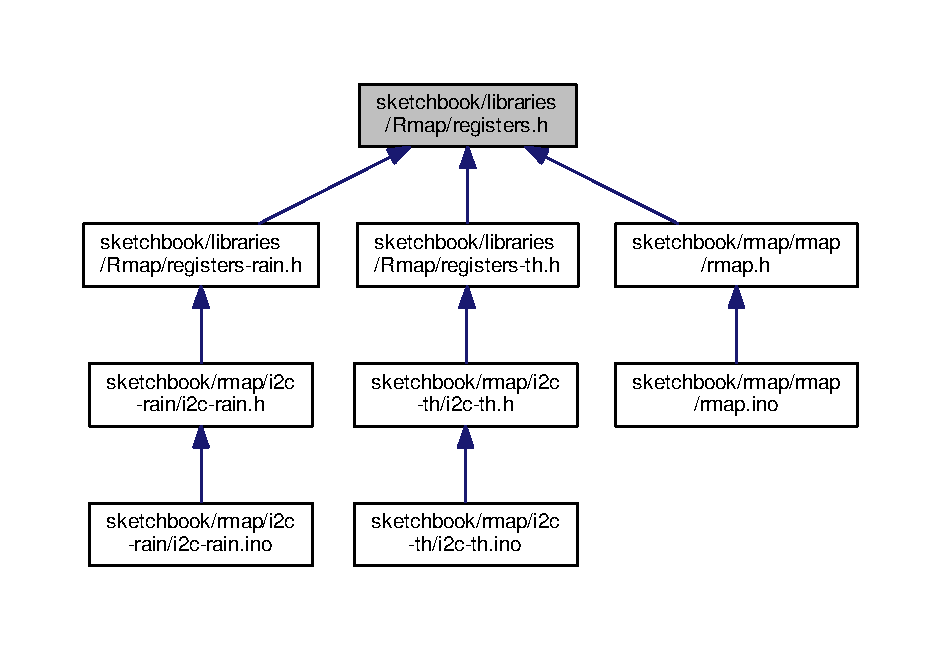
\includegraphics[width=318pt]{registers_8h__dep__incl}
\end{center}
\end{figure}
\subsection*{Macros}
\begin{DoxyCompactItemize}
\item 
\mbox{\Hypertarget{registers_8h_ad04d1b7c138bbfcc7672f00defb5f312}\label{registers_8h_ad04d1b7c138bbfcc7672f00defb5f312}} 
\#define \hyperlink{registers_8h_ad04d1b7c138bbfcc7672f00defb5f312}{I2\+C\+\_\+\+R\+E\+A\+D\+\_\+\+R\+E\+G\+I\+S\+T\+E\+R\+\_\+\+S\+T\+A\+R\+T\+\_\+\+A\+D\+D\+R\+E\+SS}~(0x00)
\begin{DoxyCompactList}\small\item\em First i2c read register address. \end{DoxyCompactList}\item 
\mbox{\Hypertarget{registers_8h_a6c89d353714d3f9241253a90808e93e6}\label{registers_8h_a6c89d353714d3f9241253a90808e93e6}} 
\#define \hyperlink{registers_8h_a6c89d353714d3f9241253a90808e93e6}{I2\+C\+\_\+\+R\+E\+A\+D\+\_\+\+R\+E\+G\+I\+S\+T\+E\+R\+\_\+\+E\+N\+D\+\_\+\+A\+D\+D\+R\+E\+SS}~(0x1\+E)
\begin{DoxyCompactList}\small\item\em Last i2c read register address. \end{DoxyCompactList}\item 
\mbox{\Hypertarget{registers_8h_ad980dee82f83659f0a84e3e1f3c177bb}\label{registers_8h_ad980dee82f83659f0a84e3e1f3c177bb}} 
\#define \hyperlink{registers_8h_ad980dee82f83659f0a84e3e1f3c177bb}{I2\+C\+\_\+\+W\+R\+I\+T\+E\+\_\+\+R\+E\+G\+I\+S\+T\+E\+R\+\_\+\+S\+T\+A\+R\+T\+\_\+\+A\+D\+D\+R\+E\+SS}~(0x1\+F)
\begin{DoxyCompactList}\small\item\em First i2c write register address. \end{DoxyCompactList}\item 
\mbox{\Hypertarget{registers_8h_a9e85c852f1a1891169a1b2db93b90b29}\label{registers_8h_a9e85c852f1a1891169a1b2db93b90b29}} 
\#define \hyperlink{registers_8h_a9e85c852f1a1891169a1b2db93b90b29}{I2\+C\+\_\+\+W\+R\+I\+T\+E\+\_\+\+R\+E\+G\+I\+S\+T\+E\+R\+\_\+\+E\+N\+D\+\_\+\+A\+D\+D\+R\+E\+SS}~(0x\+F\+E)
\begin{DoxyCompactList}\small\item\em Last i2c write register address. \end{DoxyCompactList}\item 
\mbox{\Hypertarget{registers_8h_a4398508f5478199f28b55113dd59c89e}\label{registers_8h_a4398508f5478199f28b55113dd59c89e}} 
\#define \hyperlink{registers_8h_a4398508f5478199f28b55113dd59c89e}{C\+O\+N\+F\+I\+G\+U\+R\+A\+T\+I\+O\+N\+\_\+\+E\+E\+P\+R\+O\+M\+\_\+\+A\+D\+D\+R\+E\+SS}~(0x00)
\begin{DoxyCompactList}\small\item\em First configuration register address. \end{DoxyCompactList}\item 
\mbox{\Hypertarget{registers_8h_ac14ef363cf694921e9cf4ec6ee480c47}\label{registers_8h_ac14ef363cf694921e9cf4ec6ee480c47}} 
\#define \hyperlink{registers_8h_ac14ef363cf694921e9cf4ec6ee480c47}{I2\+C\+\_\+\+C\+O\+M\+M\+A\+N\+D\+\_\+\+ID}~(0x\+F\+F)
\begin{DoxyCompactList}\small\item\em ID for i2c command. \end{DoxyCompactList}\item 
\mbox{\Hypertarget{registers_8h_a48bf9e91501e3daa29e789df9d0fc130}\label{registers_8h_a48bf9e91501e3daa29e789df9d0fc130}} 
\#define \hyperlink{registers_8h_a48bf9e91501e3daa29e789df9d0fc130}{is\+\_\+readable\+\_\+register}(register)~(register $<$= \hyperlink{registers_8h_a6c89d353714d3f9241253a90808e93e6}{I2\+C\+\_\+\+R\+E\+A\+D\+\_\+\+R\+E\+G\+I\+S\+T\+E\+R\+\_\+\+E\+N\+D\+\_\+\+A\+D\+D\+R\+E\+SS})
\begin{DoxyCompactList}\small\item\em Check if register is a readable register. \end{DoxyCompactList}\item 
\mbox{\Hypertarget{registers_8h_ad9e7ccb74eccc729a7cd7d1ef63fc98e}\label{registers_8h_ad9e7ccb74eccc729a7cd7d1ef63fc98e}} 
\#define \hyperlink{registers_8h_ad9e7ccb74eccc729a7cd7d1ef63fc98e}{is\+\_\+writable\+\_\+register}(register)~(\hyperlink{registers_8h_ad980dee82f83659f0a84e3e1f3c177bb}{I2\+C\+\_\+\+W\+R\+I\+T\+E\+\_\+\+R\+E\+G\+I\+S\+T\+E\+R\+\_\+\+S\+T\+A\+R\+T\+\_\+\+A\+D\+D\+R\+E\+SS} $<$= register \&\& register $<$= \hyperlink{registers_8h_a9e85c852f1a1891169a1b2db93b90b29}{I2\+C\+\_\+\+W\+R\+I\+T\+E\+\_\+\+R\+E\+G\+I\+S\+T\+E\+R\+\_\+\+E\+N\+D\+\_\+\+A\+D\+D\+R\+E\+SS})
\begin{DoxyCompactList}\small\item\em Check if register is a writable register. \end{DoxyCompactList}\item 
\mbox{\Hypertarget{registers_8h_ad060a6b32189d637422f26c548c31e5a}\label{registers_8h_ad060a6b32189d637422f26c548c31e5a}} 
\#define \hyperlink{registers_8h_ad060a6b32189d637422f26c548c31e5a}{is\+\_\+command}(value)~(value == \hyperlink{registers_8h_ac14ef363cf694921e9cf4ec6ee480c47}{I2\+C\+\_\+\+C\+O\+M\+M\+A\+N\+D\+\_\+\+ID})
\begin{DoxyCompactList}\small\item\em Check if value is an i2c command. \end{DoxyCompactList}\end{DoxyCompactItemize}

\hypertarget{rmap__utility_8cpp}{}\section{sketchbook/libraries/\+Rmap/rmap\+\_\+utility.cpp File Reference}
\label{rmap__utility_8cpp}\index{sketchbook/libraries/\+Rmap/rmap\+\_\+utility.\+cpp@{sketchbook/libraries/\+Rmap/rmap\+\_\+utility.\+cpp}}
{\ttfamily \#include \char`\"{}rmap\+\_\+utility.\+h\char`\"{}}\newline
{\ttfamily \#include $<$Arduino.\+h$>$}\newline
Include dependency graph for rmap\+\_\+utility.\+cpp\+:\nopagebreak
\begin{figure}[H]
\begin{center}
\leavevmode
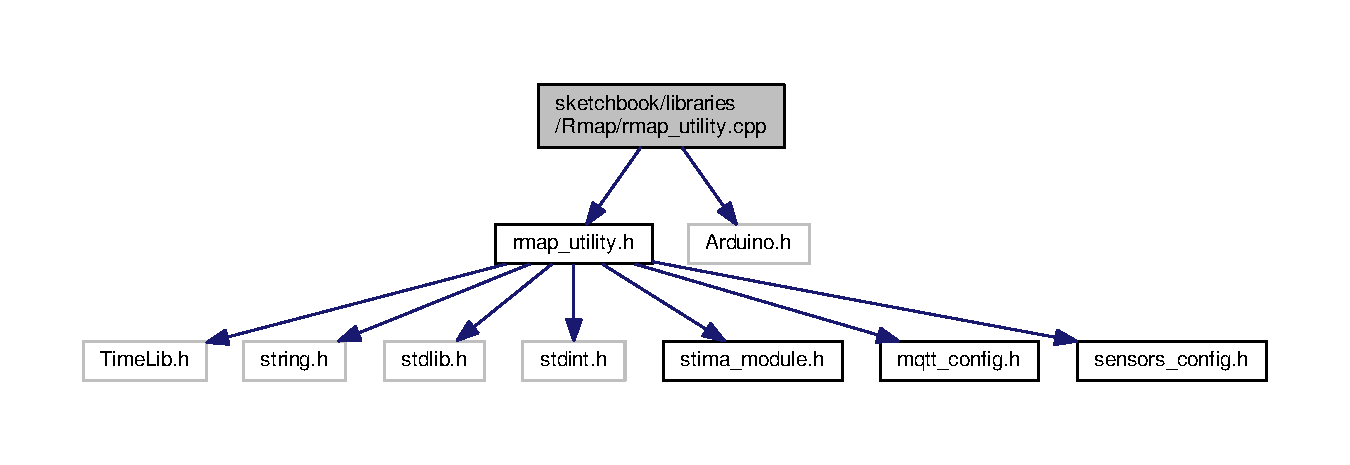
\includegraphics[width=350pt]{rmap__utility_8cpp__incl}
\end{center}
\end{figure}
\subsection*{Functions}
\begin{DoxyCompactItemize}
\item 
void \hyperlink{rmap__utility_8cpp_a243e9cf63ae67cde49acbcf4a9951288}{get\+Stima\+Name\+By\+Type} (char $\ast$name, uint8\+\_\+t type)
\begin{DoxyCompactList}\small\item\em Return a S\+T\+I\+MA\textquotesingle{}s name starting from a module type stored in configuration. \end{DoxyCompactList}\item 
void \hyperlink{rmap__utility_8cpp_a4135881294cb3a89e74548c2a706e559}{string\+To\+Array} (uint8\+\_\+t $\ast$array, char $\ast$string, const char $\ast$delimiter, uint8\+\_\+t base)
\begin{DoxyCompactList}\small\item\em Divide string in multiple value, searching by delimiter. Then convert the value in numerical format specified by base and save the values in array. \end{DoxyCompactList}\item 
void \hyperlink{rmap__utility_8cpp_aa35bbd93345decfeab85c249c5e147ce}{get\+Lon\+Lat\+From\+Mqtt\+Topic} (const char $\ast$topic, char $\ast$lon, char $\ast$lat)
\begin{DoxyCompactList}\small\item\em Extract longitue and latitude from mqtt root topic. \end{DoxyCompactList}\item 
void \hyperlink{rmap__utility_8cpp_a9603843d131fe06db8b236091877020d}{get\+Mqtt\+Client\+Id\+From\+Mqtt\+Topic} (const char $\ast$topic, char $\ast$client\+\_\+id)
\begin{DoxyCompactList}\small\item\em Extract mqtt client id from mqtt root topic. \end{DoxyCompactList}\end{DoxyCompactItemize}


\subsection{Function Documentation}
\mbox{\Hypertarget{rmap__utility_8cpp_aa35bbd93345decfeab85c249c5e147ce}\label{rmap__utility_8cpp_aa35bbd93345decfeab85c249c5e147ce}} 
\index{rmap\+\_\+utility.\+cpp@{rmap\+\_\+utility.\+cpp}!get\+Lon\+Lat\+From\+Mqtt\+Topic@{get\+Lon\+Lat\+From\+Mqtt\+Topic}}
\index{get\+Lon\+Lat\+From\+Mqtt\+Topic@{get\+Lon\+Lat\+From\+Mqtt\+Topic}!rmap\+\_\+utility.\+cpp@{rmap\+\_\+utility.\+cpp}}
\subsubsection{\texorpdfstring{get\+Lon\+Lat\+From\+Mqtt\+Topic()}{getLonLatFromMqttTopic()}}
{\footnotesize\ttfamily void get\+Lon\+Lat\+From\+Mqtt\+Topic (\begin{DoxyParamCaption}\item[{const char $\ast$}]{topic,  }\item[{char $\ast$}]{lon,  }\item[{char $\ast$}]{lat }\end{DoxyParamCaption})}



Extract longitue and latitude from mqtt root topic. 


\begin{DoxyParams}[1]{Parameters}
\mbox{\tt in}  & {\em $\ast$topic} & mqtt topic. \\
\hline
\mbox{\tt out}  & {\em $\ast$lon} & longitue buffer. \\
\hline
\mbox{\tt out}  & {\em $\ast$lat} & latitude buffer. \\
\hline
\end{DoxyParams}
\begin{DoxyReturn}{Returns}
void. 
\end{DoxyReturn}
\mbox{\Hypertarget{rmap__utility_8cpp_a9603843d131fe06db8b236091877020d}\label{rmap__utility_8cpp_a9603843d131fe06db8b236091877020d}} 
\index{rmap\+\_\+utility.\+cpp@{rmap\+\_\+utility.\+cpp}!get\+Mqtt\+Client\+Id\+From\+Mqtt\+Topic@{get\+Mqtt\+Client\+Id\+From\+Mqtt\+Topic}}
\index{get\+Mqtt\+Client\+Id\+From\+Mqtt\+Topic@{get\+Mqtt\+Client\+Id\+From\+Mqtt\+Topic}!rmap\+\_\+utility.\+cpp@{rmap\+\_\+utility.\+cpp}}
\subsubsection{\texorpdfstring{get\+Mqtt\+Client\+Id\+From\+Mqtt\+Topic()}{getMqttClientIdFromMqttTopic()}}
{\footnotesize\ttfamily void get\+Mqtt\+Client\+Id\+From\+Mqtt\+Topic (\begin{DoxyParamCaption}\item[{const char $\ast$}]{topic,  }\item[{char $\ast$}]{client\+\_\+id }\end{DoxyParamCaption})}



Extract mqtt client id from mqtt root topic. 


\begin{DoxyParams}[1]{Parameters}
\mbox{\tt in}  & {\em $\ast$topic} & mqtt topic. \\
\hline
\mbox{\tt out}  & {\em $\ast$client\+\_\+id} & mqtt client id. \\
\hline
\end{DoxyParams}
\begin{DoxyReturn}{Returns}
void. 
\end{DoxyReturn}
\mbox{\Hypertarget{rmap__utility_8cpp_a243e9cf63ae67cde49acbcf4a9951288}\label{rmap__utility_8cpp_a243e9cf63ae67cde49acbcf4a9951288}} 
\index{rmap\+\_\+utility.\+cpp@{rmap\+\_\+utility.\+cpp}!get\+Stima\+Name\+By\+Type@{get\+Stima\+Name\+By\+Type}}
\index{get\+Stima\+Name\+By\+Type@{get\+Stima\+Name\+By\+Type}!rmap\+\_\+utility.\+cpp@{rmap\+\_\+utility.\+cpp}}
\subsubsection{\texorpdfstring{get\+Stima\+Name\+By\+Type()}{getStimaNameByType()}}
{\footnotesize\ttfamily void get\+Stima\+Name\+By\+Type (\begin{DoxyParamCaption}\item[{char $\ast$}]{name,  }\item[{uint8\+\_\+t}]{type }\end{DoxyParamCaption})}



Return a S\+T\+I\+MA\textquotesingle{}s name starting from a module type stored in configuration. 


\begin{DoxyParams}[1]{Parameters}
\mbox{\tt out}  & {\em $\ast$name} & S\+T\+I\+MA\textquotesingle{}s name. \\
\hline
\mbox{\tt in}  & {\em $\ast$type} & module type stored in configuration. \\
\hline
\end{DoxyParams}
\begin{DoxyReturn}{Returns}
void. 
\end{DoxyReturn}
\mbox{\Hypertarget{rmap__utility_8cpp_a4135881294cb3a89e74548c2a706e559}\label{rmap__utility_8cpp_a4135881294cb3a89e74548c2a706e559}} 
\index{rmap\+\_\+utility.\+cpp@{rmap\+\_\+utility.\+cpp}!string\+To\+Array@{string\+To\+Array}}
\index{string\+To\+Array@{string\+To\+Array}!rmap\+\_\+utility.\+cpp@{rmap\+\_\+utility.\+cpp}}
\subsubsection{\texorpdfstring{string\+To\+Array()}{stringToArray()}}
{\footnotesize\ttfamily void string\+To\+Array (\begin{DoxyParamCaption}\item[{uint8\+\_\+t $\ast$}]{array,  }\item[{char $\ast$}]{string,  }\item[{const char $\ast$}]{delimiter,  }\item[{uint8\+\_\+t}]{base }\end{DoxyParamCaption})}



Divide string in multiple value, searching by delimiter. Then convert the value in numerical format specified by base and save the values in array. 


\begin{DoxyParams}[1]{Parameters}
\mbox{\tt out}  & {\em $\ast$array} & pointer to array obtained from string. \\
\hline
\mbox{\tt in}  & {\em $\ast$string} & source string to divide searching by delimiter. \\
\hline
\mbox{\tt in}  & {\em $\ast$delimiter} & a delimiter for divide string in multiple values. \\
\hline
\mbox{\tt in}  & {\em base} & it is a base for strtol function\+: numerical base (radix) that determines the valid characters and their interpretation. \\
\hline
\end{DoxyParams}
\begin{DoxyReturn}{Returns}
void. 
\end{DoxyReturn}

\hypertarget{rmap__utility_8h}{}\section{sketchbook/libraries/\+Rmap/rmap\+\_\+utility.h File Reference}
\label{rmap__utility_8h}\index{sketchbook/libraries/\+Rmap/rmap\+\_\+utility.\+h@{sketchbook/libraries/\+Rmap/rmap\+\_\+utility.\+h}}
{\ttfamily \#include $<$Time\+Lib.\+h$>$}\newline
{\ttfamily \#include $<$string.\+h$>$}\newline
{\ttfamily \#include $<$stdlib.\+h$>$}\newline
{\ttfamily \#include $<$stdint.\+h$>$}\newline
{\ttfamily \#include \char`\"{}stima\+\_\+module.\+h\char`\"{}}\newline
{\ttfamily \#include $<$mqtt\+\_\+config.\+h$>$}\newline
{\ttfamily \#include $<$sensors\+\_\+config.\+h$>$}\newline
Include dependency graph for rmap\+\_\+utility.\+h\+:\nopagebreak
\begin{figure}[H]
\begin{center}
\leavevmode
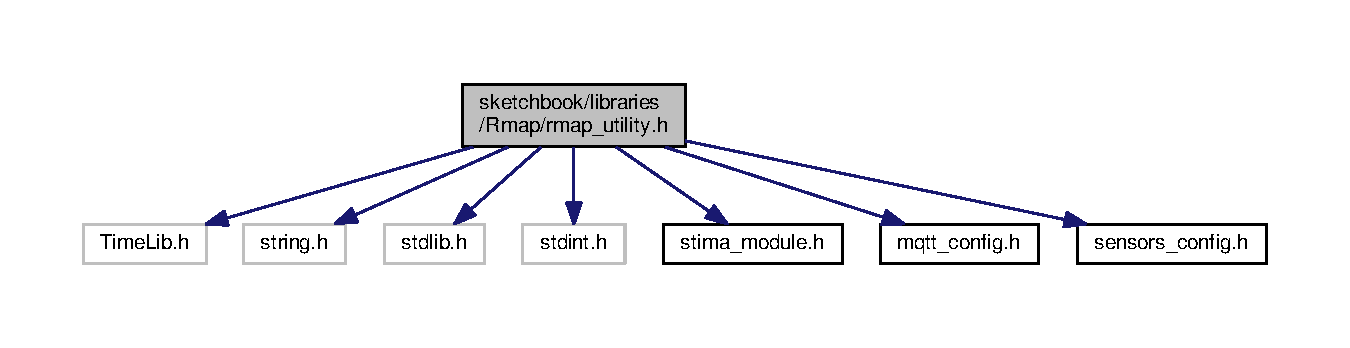
\includegraphics[width=350pt]{rmap__utility_8h__incl}
\end{center}
\end{figure}
This graph shows which files directly or indirectly include this file\+:\nopagebreak
\begin{figure}[H]
\begin{center}
\leavevmode
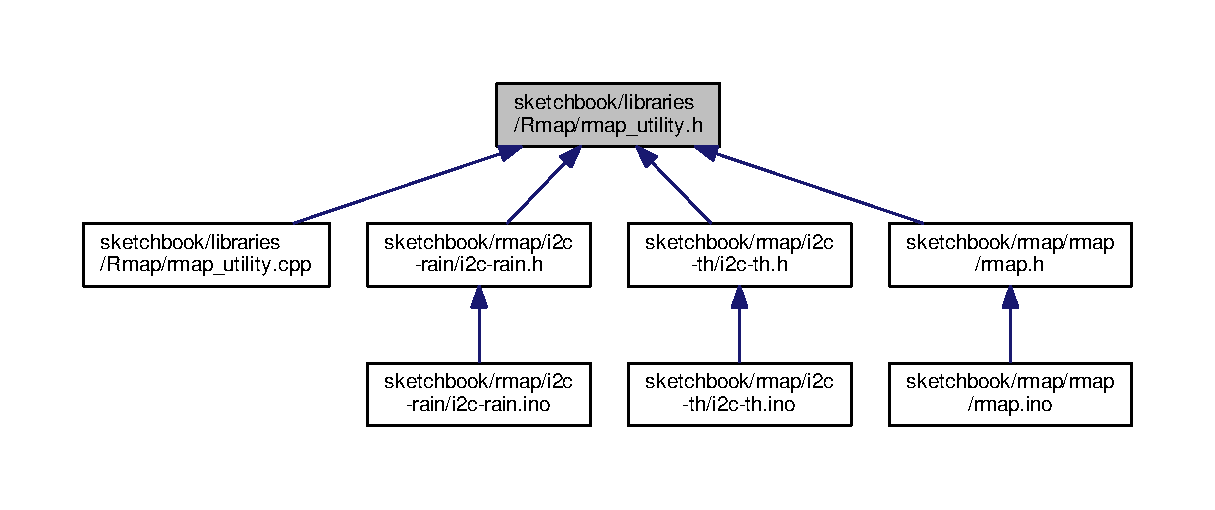
\includegraphics[width=350pt]{rmap__utility_8h__dep__incl}
\end{center}
\end{figure}
\subsection*{Macros}
\begin{DoxyCompactItemize}
\item 
\mbox{\Hypertarget{rmap__utility_8h_ae48529a4bba51677b5565dab04cbe245}\label{rmap__utility_8h_ae48529a4bba51677b5565dab04cbe245}} 
\#define \hyperlink{rmap__utility_8h_ae48529a4bba51677b5565dab04cbe245}{execute\+Timer\+Task\+Each}(current,  desidered,  offset)~(desidered \% offset == 0 ? (current \% desidered == 0 ? 1 \+: 0) \+: 0)
\begin{DoxyCompactList}\small\item\em Return true or false if current == desidered calculated in each offset. \end{DoxyCompactList}\item 
\mbox{\Hypertarget{rmap__utility_8h_a877c331bf98c513b27c382e0450426de}\label{rmap__utility_8h_a877c331bf98c513b27c382e0450426de}} 
\#define \hyperlink{rmap__utility_8h_a877c331bf98c513b27c382e0450426de}{mac\+String\+To\+Array}(mac,  string)~(\hyperlink{rmap__utility_8h_a4135881294cb3a89e74548c2a706e559}{string\+To\+Array}(mac, string, \char`\"{}\+:\char`\"{}, 16))
\begin{DoxyCompactList}\small\item\em Return an array of value rappresenting a mac address value extracted by its canonical string (xx\+:xx\+:xx\+:xx\+:xx\+:xx). \end{DoxyCompactList}\item 
\mbox{\Hypertarget{rmap__utility_8h_aff7b7a33f98123cc4d49244494cc0fc5}\label{rmap__utility_8h_aff7b7a33f98123cc4d49244494cc0fc5}} 
\#define \hyperlink{rmap__utility_8h_aff7b7a33f98123cc4d49244494cc0fc5}{ip\+String\+To\+Array}(ip,  string)~(\hyperlink{rmap__utility_8h_a4135881294cb3a89e74548c2a706e559}{string\+To\+Array}(ip, string, \char`\"{}.\char`\"{}, 10))
\begin{DoxyCompactList}\small\item\em Return an array of value rappresenting a ip address value extracted by its canonical string (xxx.\+xxx.\+xxx.\+xxx). \end{DoxyCompactList}\item 
\mbox{\Hypertarget{rmap__utility_8h_a792afe89c009b24151bfa2905c5bd6e5}\label{rmap__utility_8h_a792afe89c009b24151bfa2905c5bd6e5}} 
\#define \hyperlink{rmap__utility_8h_a792afe89c009b24151bfa2905c5bd6e5}{date\+String\+To\+Array}(date,  string)~(\hyperlink{rmap__utility_8h_a4135881294cb3a89e74548c2a706e559}{string\+To\+Array}(date, string, \char`\"{}-\/\char`\"{}, 10))
\begin{DoxyCompactList}\small\item\em Return an array of value rappresenting a date value extracted by its canonical string (xx-\/xx-\/xxxx). \end{DoxyCompactList}\item 
\mbox{\Hypertarget{rmap__utility_8h_a4ae48a415f202fc301926f041d2bb620}\label{rmap__utility_8h_a4ae48a415f202fc301926f041d2bb620}} 
\#define \hyperlink{rmap__utility_8h_a4ae48a415f202fc301926f041d2bb620}{time\+String\+To\+Array}(time,  string)~(\hyperlink{rmap__utility_8h_a4135881294cb3a89e74548c2a706e559}{string\+To\+Array}(time, string, \char`\"{}\+:\char`\"{}, 10))
\begin{DoxyCompactList}\small\item\em Return an array of value rappresenting a time value extracted by its canonical string (xx\+:xx\+:xx). \end{DoxyCompactList}\end{DoxyCompactItemize}
\subsection*{Functions}
\begin{DoxyCompactItemize}
\item 
void \hyperlink{rmap__utility_8h_a73af03c50e1c4ae36757d611e3d474f2}{mqtt\+To\+Sd} (const char $\ast$topic, const char $\ast$message, char $\ast$sd)
\begin{DoxyCompactList}\small\item\em Return a sdcard string from mqtt sensor\textquotesingle{}s topic and mqtt sensor\textquotesingle{}s value for storing on sdcard file. \end{DoxyCompactList}\item 
void \hyperlink{rmap__utility_8h_ae843b2f4240b888cfa5c747729396a2b}{sd\+To\+Mqtt} (const char $\ast$sd, char $\ast$topic, char $\ast$message)
\begin{DoxyCompactList}\small\item\em Break sdcard string in mqtt sensor\textquotesingle{}s topic and mqtt sensors\textquotesingle{} value. \end{DoxyCompactList}\item 
void \hyperlink{rmap__utility_8h_a0542c3362eb5021d4441144592783d23}{get\+Full\+Topic} (char $\ast$full\+\_\+topic, const char $\ast$root\+\_\+topic, const char $\ast$sensor\+\_\+topic)
\begin{DoxyCompactList}\small\item\em Return complete mqtt topic from root topic and sensor topic. \end{DoxyCompactList}\item 
void \hyperlink{rmap__utility_8h_a243e9cf63ae67cde49acbcf4a9951288}{get\+Stima\+Name\+By\+Type} (char $\ast$name, uint8\+\_\+t type)
\begin{DoxyCompactList}\small\item\em Return a S\+T\+I\+MA\textquotesingle{}s name starting from a module type stored in configuration. \end{DoxyCompactList}\item 
void \hyperlink{rmap__utility_8h_a4135881294cb3a89e74548c2a706e559}{string\+To\+Array} (uint8\+\_\+t $\ast$array, char $\ast$string, const char $\ast$delimiter, uint8\+\_\+t base)
\begin{DoxyCompactList}\small\item\em Divide string in multiple value, searching by delimiter. Then convert the value in numerical format specified by base and save the values in array. \end{DoxyCompactList}\item 
void \hyperlink{rmap__utility_8h_aa35bbd93345decfeab85c249c5e147ce}{get\+Lon\+Lat\+From\+Mqtt\+Topic} (const char $\ast$topic, char $\ast$lon, char $\ast$lat)
\begin{DoxyCompactList}\small\item\em Extract longitue and latitude from mqtt root topic. \end{DoxyCompactList}\item 
void \hyperlink{rmap__utility_8h_a9603843d131fe06db8b236091877020d}{get\+Mqtt\+Client\+Id\+From\+Mqtt\+Topic} (const char $\ast$topic, char $\ast$client\+\_\+id)
\begin{DoxyCompactList}\small\item\em Extract mqtt client id from mqtt root topic. \end{DoxyCompactList}\end{DoxyCompactItemize}


\subsection{Function Documentation}
\mbox{\Hypertarget{rmap__utility_8h_a0542c3362eb5021d4441144592783d23}\label{rmap__utility_8h_a0542c3362eb5021d4441144592783d23}} 
\index{rmap\+\_\+utility.\+h@{rmap\+\_\+utility.\+h}!get\+Full\+Topic@{get\+Full\+Topic}}
\index{get\+Full\+Topic@{get\+Full\+Topic}!rmap\+\_\+utility.\+h@{rmap\+\_\+utility.\+h}}
\subsubsection{\texorpdfstring{get\+Full\+Topic()}{getFullTopic()}}
{\footnotesize\ttfamily void get\+Full\+Topic (\begin{DoxyParamCaption}\item[{char $\ast$}]{full\+\_\+topic,  }\item[{const char $\ast$}]{root\+\_\+topic,  }\item[{const char $\ast$}]{sensor\+\_\+topic }\end{DoxyParamCaption})}



Return complete mqtt topic from root topic and sensor topic. 


\begin{DoxyParams}[1]{Parameters}
\mbox{\tt out}  & {\em $\ast$full\+\_\+topic} & a complete topic buffer. \\
\hline
\mbox{\tt in}  & {\em $\ast$root\+\_\+topic} & mqtt root topic (\{path\}/\{user\}/\{lon\},\{lat\}/\{typo\}/). \\
\hline
\mbox{\tt in}  & {\em $\ast$sensor\+\_\+topic} & mqtt sensor\textquotesingle{}s topic (\{aaa\},\{bbb\},\{ccc\}/\{ddd\},\{eee\},\{fff\},\{ggg\}/\+B\+X\+X\+X\+XX). \\
\hline
\end{DoxyParams}
\begin{DoxyReturn}{Returns}
void. 
\end{DoxyReturn}
\mbox{\Hypertarget{rmap__utility_8h_aa35bbd93345decfeab85c249c5e147ce}\label{rmap__utility_8h_aa35bbd93345decfeab85c249c5e147ce}} 
\index{rmap\+\_\+utility.\+h@{rmap\+\_\+utility.\+h}!get\+Lon\+Lat\+From\+Mqtt\+Topic@{get\+Lon\+Lat\+From\+Mqtt\+Topic}}
\index{get\+Lon\+Lat\+From\+Mqtt\+Topic@{get\+Lon\+Lat\+From\+Mqtt\+Topic}!rmap\+\_\+utility.\+h@{rmap\+\_\+utility.\+h}}
\subsubsection{\texorpdfstring{get\+Lon\+Lat\+From\+Mqtt\+Topic()}{getLonLatFromMqttTopic()}}
{\footnotesize\ttfamily void get\+Lon\+Lat\+From\+Mqtt\+Topic (\begin{DoxyParamCaption}\item[{const char $\ast$}]{topic,  }\item[{char $\ast$}]{lon,  }\item[{char $\ast$}]{lat }\end{DoxyParamCaption})}



Extract longitue and latitude from mqtt root topic. 


\begin{DoxyParams}[1]{Parameters}
\mbox{\tt in}  & {\em $\ast$topic} & mqtt topic. \\
\hline
\mbox{\tt out}  & {\em $\ast$lon} & longitue buffer. \\
\hline
\mbox{\tt out}  & {\em $\ast$lat} & latitude buffer. \\
\hline
\end{DoxyParams}
\begin{DoxyReturn}{Returns}
void. 
\end{DoxyReturn}
\mbox{\Hypertarget{rmap__utility_8h_a9603843d131fe06db8b236091877020d}\label{rmap__utility_8h_a9603843d131fe06db8b236091877020d}} 
\index{rmap\+\_\+utility.\+h@{rmap\+\_\+utility.\+h}!get\+Mqtt\+Client\+Id\+From\+Mqtt\+Topic@{get\+Mqtt\+Client\+Id\+From\+Mqtt\+Topic}}
\index{get\+Mqtt\+Client\+Id\+From\+Mqtt\+Topic@{get\+Mqtt\+Client\+Id\+From\+Mqtt\+Topic}!rmap\+\_\+utility.\+h@{rmap\+\_\+utility.\+h}}
\subsubsection{\texorpdfstring{get\+Mqtt\+Client\+Id\+From\+Mqtt\+Topic()}{getMqttClientIdFromMqttTopic()}}
{\footnotesize\ttfamily void get\+Mqtt\+Client\+Id\+From\+Mqtt\+Topic (\begin{DoxyParamCaption}\item[{const char $\ast$}]{topic,  }\item[{char $\ast$}]{client\+\_\+id }\end{DoxyParamCaption})}



Extract mqtt client id from mqtt root topic. 


\begin{DoxyParams}[1]{Parameters}
\mbox{\tt in}  & {\em $\ast$topic} & mqtt topic. \\
\hline
\mbox{\tt out}  & {\em $\ast$client\+\_\+id} & mqtt client id. \\
\hline
\end{DoxyParams}
\begin{DoxyReturn}{Returns}
void. 
\end{DoxyReturn}
\mbox{\Hypertarget{rmap__utility_8h_a243e9cf63ae67cde49acbcf4a9951288}\label{rmap__utility_8h_a243e9cf63ae67cde49acbcf4a9951288}} 
\index{rmap\+\_\+utility.\+h@{rmap\+\_\+utility.\+h}!get\+Stima\+Name\+By\+Type@{get\+Stima\+Name\+By\+Type}}
\index{get\+Stima\+Name\+By\+Type@{get\+Stima\+Name\+By\+Type}!rmap\+\_\+utility.\+h@{rmap\+\_\+utility.\+h}}
\subsubsection{\texorpdfstring{get\+Stima\+Name\+By\+Type()}{getStimaNameByType()}}
{\footnotesize\ttfamily void get\+Stima\+Name\+By\+Type (\begin{DoxyParamCaption}\item[{char $\ast$}]{name,  }\item[{uint8\+\_\+t}]{type }\end{DoxyParamCaption})}



Return a S\+T\+I\+MA\textquotesingle{}s name starting from a module type stored in configuration. 


\begin{DoxyParams}[1]{Parameters}
\mbox{\tt out}  & {\em $\ast$name} & S\+T\+I\+MA\textquotesingle{}s name. \\
\hline
\mbox{\tt in}  & {\em $\ast$type} & module type stored in configuration. \\
\hline
\end{DoxyParams}
\begin{DoxyReturn}{Returns}
void. 
\end{DoxyReturn}
\mbox{\Hypertarget{rmap__utility_8h_a73af03c50e1c4ae36757d611e3d474f2}\label{rmap__utility_8h_a73af03c50e1c4ae36757d611e3d474f2}} 
\index{rmap\+\_\+utility.\+h@{rmap\+\_\+utility.\+h}!mqtt\+To\+Sd@{mqtt\+To\+Sd}}
\index{mqtt\+To\+Sd@{mqtt\+To\+Sd}!rmap\+\_\+utility.\+h@{rmap\+\_\+utility.\+h}}
\subsubsection{\texorpdfstring{mqtt\+To\+Sd()}{mqttToSd()}}
{\footnotesize\ttfamily void mqtt\+To\+Sd (\begin{DoxyParamCaption}\item[{const char $\ast$}]{topic,  }\item[{const char $\ast$}]{message,  }\item[{char $\ast$}]{sd }\end{DoxyParamCaption})}



Return a sdcard string from mqtt sensor\textquotesingle{}s topic and mqtt sensor\textquotesingle{}s value for storing on sdcard file. 


\begin{DoxyParams}[1]{Parameters}
\mbox{\tt in}  & {\em $\ast$topic} & full mqtt sensor\textquotesingle{}s topic (\{path\}/\{user\}/\{lon\},\{lat\}/\{typo\}/\{aaa\},\{bbb\},\{ccc\}/\{ddd\},\{eee\},\{fff\},\{ggg\}/\+B\+X\+X\+X\+XX) \\
\hline
\mbox{\tt in}  & {\em $\ast$message} & mqtt sensor\textquotesingle{}s value. \\
\hline
\mbox{\tt out}  & {\em $\ast$sd} & sdcard string (\{aaa\},\{bbb\},\{ccc\}/\{ddd\},\{eee\},\{fff\},\{ggg\}/\+B\+X\+X\+X\+XX \{\char`\"{}v\char`\"{}\+:xxx,\char`\"{}t\char`\"{}\+:\char`\"{}yyyy-\/mm-\/dd\+T\+H\+H\+:\+M\+M\+:\+S\+S\char`\"{}\}). \\
\hline
\end{DoxyParams}
\begin{DoxyReturn}{Returns}
void. 
\end{DoxyReturn}
\mbox{\Hypertarget{rmap__utility_8h_ae843b2f4240b888cfa5c747729396a2b}\label{rmap__utility_8h_ae843b2f4240b888cfa5c747729396a2b}} 
\index{rmap\+\_\+utility.\+h@{rmap\+\_\+utility.\+h}!sd\+To\+Mqtt@{sd\+To\+Mqtt}}
\index{sd\+To\+Mqtt@{sd\+To\+Mqtt}!rmap\+\_\+utility.\+h@{rmap\+\_\+utility.\+h}}
\subsubsection{\texorpdfstring{sd\+To\+Mqtt()}{sdToMqtt()}}
{\footnotesize\ttfamily void sd\+To\+Mqtt (\begin{DoxyParamCaption}\item[{const char $\ast$}]{sd,  }\item[{char $\ast$}]{topic,  }\item[{char $\ast$}]{message }\end{DoxyParamCaption})}



Break sdcard string in mqtt sensor\textquotesingle{}s topic and mqtt sensors\textquotesingle{} value. 


\begin{DoxyParams}[1]{Parameters}
\mbox{\tt in}  & {\em $\ast$sd} & sdcard string (\{aaa\},\{bbb\},\{ccc\}/\{ddd\},\{eee\},\{fff\},\{ggg\}/\+B\+X\+X\+X\+XX \{\char`\"{}v\char`\"{}\+:xxx,\char`\"{}t\char`\"{}\+:\char`\"{}yyyy-\/mm-\/dd\+T\+H\+H\+:\+M\+M\+:\+S\+S\char`\"{}\}). \\
\hline
\mbox{\tt out}  & {\em $\ast$topic} & mqtt sensor\textquotesingle{}s topic (\{aaa\},\{bbb\},\{ccc\}/\{ddd\},\{eee\},\{fff\},\{ggg\}/\+B\+X\+X\+X\+XX). \\
\hline
\mbox{\tt out}  & {\em $\ast$message} & mqtt sensor\textquotesingle{}s topic (\{\char`\"{}v\char`\"{}\+:xxx,\char`\"{}t\char`\"{}\+:\char`\"{}yyyy-\/mm-\/dd\+T\+H\+H\+:\+M\+M\+:\+S\+S\char`\"{}\}). \\
\hline
\end{DoxyParams}
\begin{DoxyReturn}{Returns}
void. 
\end{DoxyReturn}
\mbox{\Hypertarget{rmap__utility_8h_a4135881294cb3a89e74548c2a706e559}\label{rmap__utility_8h_a4135881294cb3a89e74548c2a706e559}} 
\index{rmap\+\_\+utility.\+h@{rmap\+\_\+utility.\+h}!string\+To\+Array@{string\+To\+Array}}
\index{string\+To\+Array@{string\+To\+Array}!rmap\+\_\+utility.\+h@{rmap\+\_\+utility.\+h}}
\subsubsection{\texorpdfstring{string\+To\+Array()}{stringToArray()}}
{\footnotesize\ttfamily void string\+To\+Array (\begin{DoxyParamCaption}\item[{uint8\+\_\+t $\ast$}]{array,  }\item[{char $\ast$}]{string,  }\item[{const char $\ast$}]{delimiter,  }\item[{uint8\+\_\+t}]{base }\end{DoxyParamCaption})}



Divide string in multiple value, searching by delimiter. Then convert the value in numerical format specified by base and save the values in array. 


\begin{DoxyParams}[1]{Parameters}
\mbox{\tt out}  & {\em $\ast$array} & pointer to array obtained from string. \\
\hline
\mbox{\tt in}  & {\em $\ast$string} & source string to divide searching by delimiter. \\
\hline
\mbox{\tt in}  & {\em $\ast$delimiter} & a delimiter for divide string in multiple values. \\
\hline
\mbox{\tt in}  & {\em base} & it is a base for strtol function\+: numerical base (radix) that determines the valid characters and their interpretation. \\
\hline
\end{DoxyParams}
\begin{DoxyReturn}{Returns}
void. 
\end{DoxyReturn}

\hypertarget{sdcard__utility_8cpp}{}\section{sketchbook/libraries/\+Rmap/sdcard\+\_\+utility.cpp File Reference}
\label{sdcard__utility_8cpp}\index{sketchbook/libraries/\+Rmap/sdcard\+\_\+utility.\+cpp@{sketchbook/libraries/\+Rmap/sdcard\+\_\+utility.\+cpp}}
{\ttfamily \#include \char`\"{}sdcard\+\_\+utility.\+h\char`\"{}}\newline
Include dependency graph for sdcard\+\_\+utility.\+cpp\+:\nopagebreak
\begin{figure}[H]
\begin{center}
\leavevmode
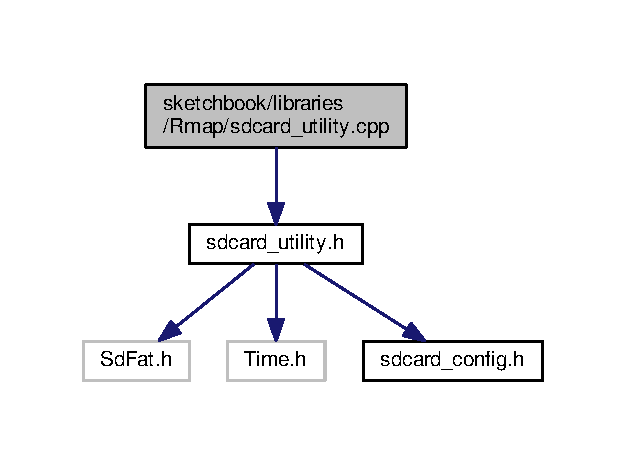
\includegraphics[width=301pt]{sdcard__utility_8cpp__incl}
\end{center}
\end{figure}
\subsection*{Functions}
\begin{DoxyCompactItemize}
\item 
bool \hyperlink{sdcard__utility_8cpp_a9375a6f4bfaff011d92f7cbbc8facba6}{sdcard\+\_\+init} (Sd\+Fat $\ast$SD, uint8\+\_\+t chip\+\_\+select)
\begin{DoxyCompactList}\small\item\em Init sdcard and check if operation was succesful. \end{DoxyCompactList}\item 
bool \hyperlink{sdcard__utility_8cpp_ac5dafadabc1474a4dd75ceaf002d0c91}{sdcard\+\_\+open\+\_\+file} (Sd\+Fat $\ast$SD, File $\ast$file, const char $\ast$file\+\_\+name, uint8\+\_\+t param)
\begin{DoxyCompactList}\small\item\em Open file on sdcard with relative file mode bits. \end{DoxyCompactList}\item 
void \hyperlink{sdcard__utility_8cpp_aa9384608e9f039f0deda9438277383cc}{sdcard\+\_\+make\+\_\+filename} (time\+\_\+t time, char $\ast$file\+\_\+name)
\begin{DoxyCompactList}\small\item\em Generate a file name (dd\+\_\+mm\+\_\+yyyy.\+txt) starting from a variable containing a seconds elapsed from 00\+:00\+:00 01/01/1900. \end{DoxyCompactList}\end{DoxyCompactItemize}


\subsection{Function Documentation}
\mbox{\Hypertarget{sdcard__utility_8cpp_a9375a6f4bfaff011d92f7cbbc8facba6}\label{sdcard__utility_8cpp_a9375a6f4bfaff011d92f7cbbc8facba6}} 
\index{sdcard\+\_\+utility.\+cpp@{sdcard\+\_\+utility.\+cpp}!sdcard\+\_\+init@{sdcard\+\_\+init}}
\index{sdcard\+\_\+init@{sdcard\+\_\+init}!sdcard\+\_\+utility.\+cpp@{sdcard\+\_\+utility.\+cpp}}
\subsubsection{\texorpdfstring{sdcard\+\_\+init()}{sdcard\_init()}}
{\footnotesize\ttfamily bool sdcard\+\_\+init (\begin{DoxyParamCaption}\item[{Sd\+Fat $\ast$}]{SD,  }\item[{uint8\+\_\+t}]{chip\+\_\+select }\end{DoxyParamCaption})}



Init sdcard and check if operation was succesful. 


\begin{DoxyParams}[1]{Parameters}
\mbox{\tt in}  & {\em $\ast$\+SD} & pointer to sdcard instance. \\
\hline
\mbox{\tt in}  & {\em chip\+\_\+select} & corresponding chip select pin. \\
\hline
\end{DoxyParams}
\begin{DoxyReturn}{Returns}
true if success, false otherwise. 
\end{DoxyReturn}
\mbox{\Hypertarget{sdcard__utility_8cpp_aa9384608e9f039f0deda9438277383cc}\label{sdcard__utility_8cpp_aa9384608e9f039f0deda9438277383cc}} 
\index{sdcard\+\_\+utility.\+cpp@{sdcard\+\_\+utility.\+cpp}!sdcard\+\_\+make\+\_\+filename@{sdcard\+\_\+make\+\_\+filename}}
\index{sdcard\+\_\+make\+\_\+filename@{sdcard\+\_\+make\+\_\+filename}!sdcard\+\_\+utility.\+cpp@{sdcard\+\_\+utility.\+cpp}}
\subsubsection{\texorpdfstring{sdcard\+\_\+make\+\_\+filename()}{sdcard\_make\_filename()}}
{\footnotesize\ttfamily void sdcard\+\_\+make\+\_\+filename (\begin{DoxyParamCaption}\item[{time\+\_\+t}]{time,  }\item[{char $\ast$}]{file\+\_\+name }\end{DoxyParamCaption})}



Generate a file name (dd\+\_\+mm\+\_\+yyyy.\+txt) starting from a variable containing a seconds elapsed from 00\+:00\+:00 01/01/1900. 


\begin{DoxyParams}[1]{Parameters}
\mbox{\tt in}  & {\em $\ast$time} & seconds since 1900. \\
\hline
\mbox{\tt out}  & {\em $\ast$file\+\_\+name} & file name generated from time. \\
\hline
\end{DoxyParams}
\begin{DoxyReturn}{Returns}
void. 
\end{DoxyReturn}
\mbox{\Hypertarget{sdcard__utility_8cpp_ac5dafadabc1474a4dd75ceaf002d0c91}\label{sdcard__utility_8cpp_ac5dafadabc1474a4dd75ceaf002d0c91}} 
\index{sdcard\+\_\+utility.\+cpp@{sdcard\+\_\+utility.\+cpp}!sdcard\+\_\+open\+\_\+file@{sdcard\+\_\+open\+\_\+file}}
\index{sdcard\+\_\+open\+\_\+file@{sdcard\+\_\+open\+\_\+file}!sdcard\+\_\+utility.\+cpp@{sdcard\+\_\+utility.\+cpp}}
\subsubsection{\texorpdfstring{sdcard\+\_\+open\+\_\+file()}{sdcard\_open\_file()}}
{\footnotesize\ttfamily bool sdcard\+\_\+open\+\_\+file (\begin{DoxyParamCaption}\item[{Sd\+Fat $\ast$}]{SD,  }\item[{File $\ast$}]{file,  }\item[{const char $\ast$}]{file\+\_\+name,  }\item[{uint8\+\_\+t}]{param }\end{DoxyParamCaption})}



Open file on sdcard with relative file mode bits. 


\begin{DoxyParams}[1]{Parameters}
\mbox{\tt in}  & {\em $\ast$\+SD} & pointer to sdcard instance. \\
\hline
\mbox{\tt in}  & {\em $\ast$file} & pointer to file instance. \\
\hline
\mbox{\tt in}  & {\em $\ast$file\+\_\+name} & file name. \\
\hline
\mbox{\tt in}  & {\em param} & parameter for open file (example\+: O\+\_\+\+R\+D\+WR $\vert$ O\+\_\+\+C\+R\+E\+AT $\vert$ O\+\_\+\+A\+P\+P\+E\+ND. See Sd\+Fat documentation). \\
\hline
\end{DoxyParams}
\begin{DoxyReturn}{Returns}
true if success, false otherwise. 
\end{DoxyReturn}

\hypertarget{sdcard__utility_8h}{}\section{sketchbook/libraries/\+Rmap/sdcard\+\_\+utility.h File Reference}
\label{sdcard__utility_8h}\index{sketchbook/libraries/\+Rmap/sdcard\+\_\+utility.\+h@{sketchbook/libraries/\+Rmap/sdcard\+\_\+utility.\+h}}
{\ttfamily \#include $<$Sd\+Fat.\+h$>$}\newline
{\ttfamily \#include $<$Time.\+h$>$}\newline
{\ttfamily \#include $<$sdcard\+\_\+config.\+h$>$}\newline
Include dependency graph for sdcard\+\_\+utility.\+h\+:\nopagebreak
\begin{figure}[H]
\begin{center}
\leavevmode
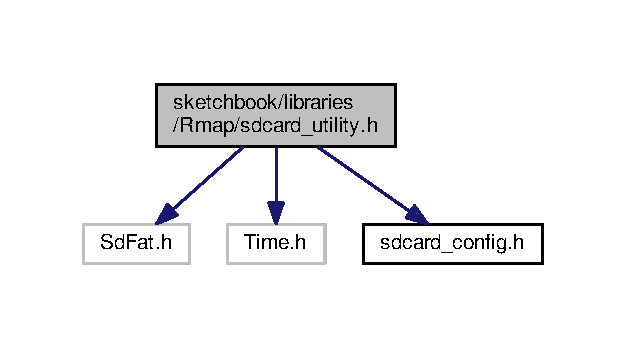
\includegraphics[width=301pt]{sdcard__utility_8h__incl}
\end{center}
\end{figure}
This graph shows which files directly or indirectly include this file\+:\nopagebreak
\begin{figure}[H]
\begin{center}
\leavevmode
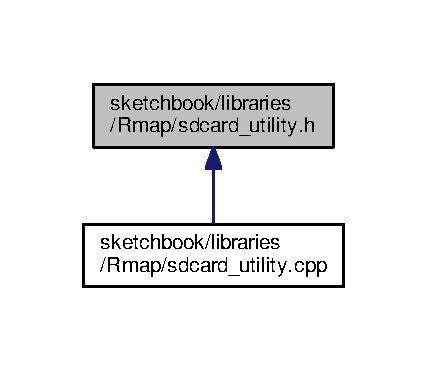
\includegraphics[width=340pt]{sdcard__utility_8h__dep__incl}
\end{center}
\end{figure}
\subsection*{Functions}
\begin{DoxyCompactItemize}
\item 
bool \hyperlink{sdcard__utility_8h_a9375a6f4bfaff011d92f7cbbc8facba6}{sdcard\+\_\+init} (Sd\+Fat $\ast$SD, uint8\+\_\+t chip\+\_\+select)
\begin{DoxyCompactList}\small\item\em Init sdcard and check if operation was succesful. \end{DoxyCompactList}\item 
bool \hyperlink{sdcard__utility_8h_ac5dafadabc1474a4dd75ceaf002d0c91}{sdcard\+\_\+open\+\_\+file} (Sd\+Fat $\ast$SD, File $\ast$file, const char $\ast$file\+\_\+name, uint8\+\_\+t param)
\begin{DoxyCompactList}\small\item\em Open file on sdcard with relative file mode bits. \end{DoxyCompactList}\item 
void \hyperlink{sdcard__utility_8h_aa9384608e9f039f0deda9438277383cc}{sdcard\+\_\+make\+\_\+filename} (time\+\_\+t time, char $\ast$file\+\_\+name)
\begin{DoxyCompactList}\small\item\em Generate a file name (dd\+\_\+mm\+\_\+yyyy.\+txt) starting from a variable containing a seconds elapsed from 00\+:00\+:00 01/01/1900. \end{DoxyCompactList}\end{DoxyCompactItemize}


\subsection{Function Documentation}
\mbox{\Hypertarget{sdcard__utility_8h_a9375a6f4bfaff011d92f7cbbc8facba6}\label{sdcard__utility_8h_a9375a6f4bfaff011d92f7cbbc8facba6}} 
\index{sdcard\+\_\+utility.\+h@{sdcard\+\_\+utility.\+h}!sdcard\+\_\+init@{sdcard\+\_\+init}}
\index{sdcard\+\_\+init@{sdcard\+\_\+init}!sdcard\+\_\+utility.\+h@{sdcard\+\_\+utility.\+h}}
\subsubsection{\texorpdfstring{sdcard\+\_\+init()}{sdcard\_init()}}
{\footnotesize\ttfamily bool sdcard\+\_\+init (\begin{DoxyParamCaption}\item[{Sd\+Fat $\ast$}]{SD,  }\item[{uint8\+\_\+t}]{chip\+\_\+select }\end{DoxyParamCaption})}



Init sdcard and check if operation was succesful. 


\begin{DoxyParams}[1]{Parameters}
\mbox{\tt in}  & {\em $\ast$\+SD} & pointer to sdcard instance. \\
\hline
\mbox{\tt in}  & {\em chip\+\_\+select} & corresponding chip select pin. \\
\hline
\end{DoxyParams}
\begin{DoxyReturn}{Returns}
true if success, false otherwise. 
\end{DoxyReturn}
\mbox{\Hypertarget{sdcard__utility_8h_aa9384608e9f039f0deda9438277383cc}\label{sdcard__utility_8h_aa9384608e9f039f0deda9438277383cc}} 
\index{sdcard\+\_\+utility.\+h@{sdcard\+\_\+utility.\+h}!sdcard\+\_\+make\+\_\+filename@{sdcard\+\_\+make\+\_\+filename}}
\index{sdcard\+\_\+make\+\_\+filename@{sdcard\+\_\+make\+\_\+filename}!sdcard\+\_\+utility.\+h@{sdcard\+\_\+utility.\+h}}
\subsubsection{\texorpdfstring{sdcard\+\_\+make\+\_\+filename()}{sdcard\_make\_filename()}}
{\footnotesize\ttfamily void sdcard\+\_\+make\+\_\+filename (\begin{DoxyParamCaption}\item[{time\+\_\+t}]{time,  }\item[{char $\ast$}]{file\+\_\+name }\end{DoxyParamCaption})}



Generate a file name (dd\+\_\+mm\+\_\+yyyy.\+txt) starting from a variable containing a seconds elapsed from 00\+:00\+:00 01/01/1900. 


\begin{DoxyParams}[1]{Parameters}
\mbox{\tt in}  & {\em $\ast$time} & seconds since 1900. \\
\hline
\mbox{\tt out}  & {\em $\ast$file\+\_\+name} & file name generated from time. \\
\hline
\end{DoxyParams}
\begin{DoxyReturn}{Returns}
void. 
\end{DoxyReturn}
\mbox{\Hypertarget{sdcard__utility_8h_ac5dafadabc1474a4dd75ceaf002d0c91}\label{sdcard__utility_8h_ac5dafadabc1474a4dd75ceaf002d0c91}} 
\index{sdcard\+\_\+utility.\+h@{sdcard\+\_\+utility.\+h}!sdcard\+\_\+open\+\_\+file@{sdcard\+\_\+open\+\_\+file}}
\index{sdcard\+\_\+open\+\_\+file@{sdcard\+\_\+open\+\_\+file}!sdcard\+\_\+utility.\+h@{sdcard\+\_\+utility.\+h}}
\subsubsection{\texorpdfstring{sdcard\+\_\+open\+\_\+file()}{sdcard\_open\_file()}}
{\footnotesize\ttfamily bool sdcard\+\_\+open\+\_\+file (\begin{DoxyParamCaption}\item[{Sd\+Fat $\ast$}]{SD,  }\item[{File $\ast$}]{file,  }\item[{const char $\ast$}]{file\+\_\+name,  }\item[{uint8\+\_\+t}]{param }\end{DoxyParamCaption})}



Open file on sdcard with relative file mode bits. 


\begin{DoxyParams}[1]{Parameters}
\mbox{\tt in}  & {\em $\ast$\+SD} & pointer to sdcard instance. \\
\hline
\mbox{\tt in}  & {\em $\ast$file} & pointer to file instance. \\
\hline
\mbox{\tt in}  & {\em $\ast$file\+\_\+name} & file name. \\
\hline
\mbox{\tt in}  & {\em param} & parameter for open file (example\+: O\+\_\+\+R\+D\+WR $\vert$ O\+\_\+\+C\+R\+E\+AT $\vert$ O\+\_\+\+A\+P\+P\+E\+ND. See Sd\+Fat documentation). \\
\hline
\end{DoxyParams}
\begin{DoxyReturn}{Returns}
true if success, false otherwise. 
\end{DoxyReturn}

\hypertarget{stima__module_8h}{}\section{sketchbook/libraries/\+Rmap/stima\+\_\+module.h File Reference}
\label{stima__module_8h}\index{sketchbook/libraries/\+Rmap/stima\+\_\+module.\+h@{sketchbook/libraries/\+Rmap/stima\+\_\+module.\+h}}
This graph shows which files directly or indirectly include this file\+:\nopagebreak
\begin{figure}[H]
\begin{center}
\leavevmode
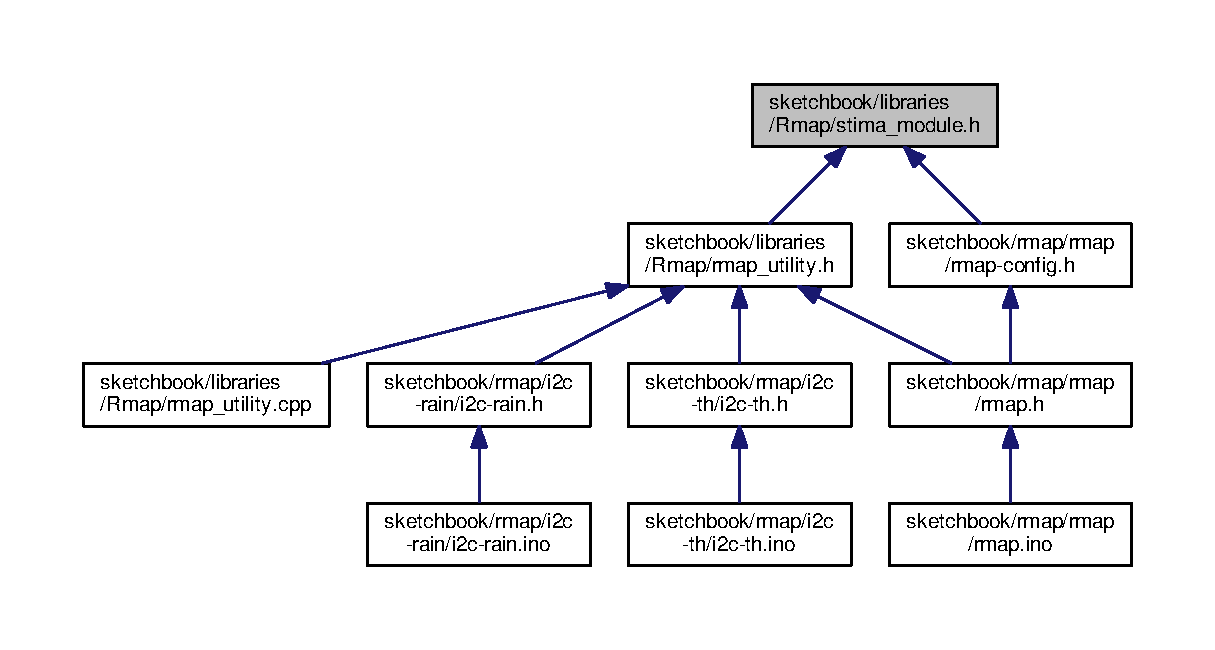
\includegraphics[width=350pt]{stima__module_8h__dep__incl}
\end{center}
\end{figure}
\subsection*{Macros}
\begin{DoxyCompactItemize}
\item 
\mbox{\Hypertarget{stima__module_8h_a3398e472ac79f3fce3d40212a0b2d1c0}\label{stima__module_8h_a3398e472ac79f3fce3d40212a0b2d1c0}} 
\#define \hyperlink{stima__module_8h_a3398e472ac79f3fce3d40212a0b2d1c0}{C\+O\+N\+F\+I\+G\+U\+R\+A\+T\+I\+O\+N\+\_\+\+C\+U\+R\+R\+E\+NT}~(0)
\begin{DoxyCompactList}\small\item\em Indicate current configuration. \end{DoxyCompactList}\item 
\mbox{\Hypertarget{stima__module_8h_ae0aa5ba1e9ac4f3efa2292f0de6fbe7b}\label{stima__module_8h_ae0aa5ba1e9ac4f3efa2292f0de6fbe7b}} 
\#define \hyperlink{stima__module_8h_ae0aa5ba1e9ac4f3efa2292f0de6fbe7b}{C\+O\+N\+F\+I\+G\+U\+R\+A\+T\+I\+O\+N\+\_\+\+D\+E\+F\+A\+U\+LT}~(1)
\begin{DoxyCompactList}\small\item\em Indicate default configuration. \end{DoxyCompactList}\item 
\mbox{\Hypertarget{stima__module_8h_a23345b20705c087da0c9327c5191749e}\label{stima__module_8h_a23345b20705c087da0c9327c5191749e}} 
\#define \hyperlink{stima__module_8h_a23345b20705c087da0c9327c5191749e}{S\+T\+I\+M\+A\+\_\+\+M\+O\+D\+U\+L\+E\+\_\+\+T\+Y\+P\+E\+\_\+\+S\+A\+M\+P\+L\+E\+\_\+\+E\+TH}~(1)
\begin{DoxyCompactList}\small\item\em The module send sample over ethernet. \end{DoxyCompactList}\item 
\mbox{\Hypertarget{stima__module_8h_aeee56ac5cd6b4aa0079097e530b1c27c}\label{stima__module_8h_aeee56ac5cd6b4aa0079097e530b1c27c}} 
\#define \hyperlink{stima__module_8h_aeee56ac5cd6b4aa0079097e530b1c27c}{S\+T\+I\+M\+A\+\_\+\+M\+O\+D\+U\+L\+E\+\_\+\+T\+Y\+P\+E\+\_\+\+R\+E\+P\+O\+R\+T\+\_\+\+E\+TH}~(2)
\begin{DoxyCompactList}\small\item\em The module send report over ethernet. \end{DoxyCompactList}\item 
\mbox{\Hypertarget{stima__module_8h_a74dc1572ea816fbe8d7018923f6eedc9}\label{stima__module_8h_a74dc1572ea816fbe8d7018923f6eedc9}} 
\#define \hyperlink{stima__module_8h_a74dc1572ea816fbe8d7018923f6eedc9}{S\+T\+I\+M\+A\+\_\+\+M\+O\+D\+U\+L\+E\+\_\+\+T\+Y\+P\+E\+\_\+\+S\+A\+M\+P\+L\+E\+\_\+\+G\+SM}~(3)
\begin{DoxyCompactList}\small\item\em The module send sample over gsm/gprs. \end{DoxyCompactList}\item 
\mbox{\Hypertarget{stima__module_8h_aea131800c42cd2037b9a227f49d65872}\label{stima__module_8h_aea131800c42cd2037b9a227f49d65872}} 
\#define \hyperlink{stima__module_8h_aea131800c42cd2037b9a227f49d65872}{S\+T\+I\+M\+A\+\_\+\+M\+O\+D\+U\+L\+E\+\_\+\+T\+Y\+P\+E\+\_\+\+R\+E\+P\+O\+R\+T\+\_\+\+G\+SM}~(4)
\begin{DoxyCompactList}\small\item\em The module send report over gsm/gprs. \end{DoxyCompactList}\item 
\mbox{\Hypertarget{stima__module_8h_a4943971f8bec57e337e3f40f085b7fa3}\label{stima__module_8h_a4943971f8bec57e337e3f40f085b7fa3}} 
\#define \hyperlink{stima__module_8h_a4943971f8bec57e337e3f40f085b7fa3}{S\+T\+I\+M\+A\+\_\+\+M\+O\+D\+U\+L\+E\+\_\+\+T\+Y\+P\+E\+\_\+\+R\+A\+IN}~(5)
\begin{DoxyCompactList}\small\item\em The module acquire rain tips. \end{DoxyCompactList}\item 
\mbox{\Hypertarget{stima__module_8h_ab4d075291417ea1254b52a2db807c89d}\label{stima__module_8h_ab4d075291417ea1254b52a2db807c89d}} 
\#define \hyperlink{stima__module_8h_ab4d075291417ea1254b52a2db807c89d}{S\+T\+I\+M\+A\+\_\+\+M\+O\+D\+U\+L\+E\+\_\+\+T\+Y\+P\+E\+\_\+\+TH}~(6)
\begin{DoxyCompactList}\small\item\em The module acquire temperature and humidity. \end{DoxyCompactList}\item 
\mbox{\Hypertarget{stima__module_8h_ab834479c01735f15f5d599365b95c837}\label{stima__module_8h_ab834479c01735f15f5d599365b95c837}} 
\#define \hyperlink{stima__module_8h_ab834479c01735f15f5d599365b95c837}{S\+T\+I\+M\+A\+\_\+\+M\+O\+D\+U\+L\+E\+\_\+\+T\+Y\+P\+E\+\_\+\+P\+A\+S\+S\+I\+V\+E\+\_\+\+E\+TH}~(7)
\begin{DoxyCompactList}\small\item\em Module in passive mode. \end{DoxyCompactList}\item 
\mbox{\Hypertarget{stima__module_8h_a3797fcb3c310092d8bb4220634b79b22}\label{stima__module_8h_a3797fcb3c310092d8bb4220634b79b22}} 
\#define \hyperlink{stima__module_8h_a3797fcb3c310092d8bb4220634b79b22}{S\+T\+I\+M\+A\+\_\+\+M\+O\+D\+U\+L\+E\+\_\+\+T\+Y\+P\+E\+\_\+\+P\+A\+S\+S\+I\+V\+E\+\_\+\+G\+SM}~(8)
\begin{DoxyCompactList}\small\item\em Module in passive mode. \end{DoxyCompactList}\item 
\mbox{\Hypertarget{stima__module_8h_a38851bfc5882fc89e22af5dae1b36564}\label{stima__module_8h_a38851bfc5882fc89e22af5dae1b36564}} 
\#define \hyperlink{stima__module_8h_a38851bfc5882fc89e22af5dae1b36564}{S\+T\+I\+M\+A\+\_\+\+M\+O\+D\+U\+L\+E\+\_\+\+T\+Y\+P\+E\+\_\+\+P\+A\+S\+S\+I\+VE}~(9)
\begin{DoxyCompactList}\small\item\em Module in passive mode. \end{DoxyCompactList}\item 
\mbox{\Hypertarget{stima__module_8h_ace851f565c06bb83d8f0c2f1c7a7d04f}\label{stima__module_8h_ace851f565c06bb83d8f0c2f1c7a7d04f}} 
\#define \hyperlink{stima__module_8h_ace851f565c06bb83d8f0c2f1c7a7d04f}{S\+T\+I\+M\+A\+\_\+\+M\+O\+D\+U\+L\+E\+\_\+\+N\+A\+M\+E\+\_\+\+S\+A\+M\+P\+L\+E\+\_\+\+E\+TH}~(\char`\"{}sample-\/eth\char`\"{})
\begin{DoxyCompactList}\small\item\em The module\textquotesingle{}name for sending sample over ethernet. \end{DoxyCompactList}\item 
\mbox{\Hypertarget{stima__module_8h_a2683dff47640d9fc1e4f7b0635149276}\label{stima__module_8h_a2683dff47640d9fc1e4f7b0635149276}} 
\#define \hyperlink{stima__module_8h_a2683dff47640d9fc1e4f7b0635149276}{S\+T\+I\+M\+A\+\_\+\+M\+O\+D\+U\+L\+E\+\_\+\+N\+A\+M\+E\+\_\+\+R\+E\+P\+O\+R\+T\+\_\+\+E\+TH}~(\char`\"{}report-\/eth\char`\"{})
\begin{DoxyCompactList}\small\item\em The module\textquotesingle{}name for sending report over ethernet. \end{DoxyCompactList}\item 
\mbox{\Hypertarget{stima__module_8h_a165e074c9766ab0ae6686d5bbc95dbfd}\label{stima__module_8h_a165e074c9766ab0ae6686d5bbc95dbfd}} 
\#define \hyperlink{stima__module_8h_a165e074c9766ab0ae6686d5bbc95dbfd}{S\+T\+I\+M\+A\+\_\+\+M\+O\+D\+U\+L\+E\+\_\+\+N\+A\+M\+E\+\_\+\+S\+A\+M\+P\+L\+E\+\_\+\+G\+SM}~(\char`\"{}sample-\/gsm\char`\"{})
\begin{DoxyCompactList}\small\item\em The module\textquotesingle{}name for sending sample over gsm/gprs. \end{DoxyCompactList}\item 
\mbox{\Hypertarget{stima__module_8h_ac8eacfe0a9b3c2a5ceb382a0611d7ffa}\label{stima__module_8h_ac8eacfe0a9b3c2a5ceb382a0611d7ffa}} 
\#define \hyperlink{stima__module_8h_ac8eacfe0a9b3c2a5ceb382a0611d7ffa}{S\+T\+I\+M\+A\+\_\+\+M\+O\+D\+U\+L\+E\+\_\+\+N\+A\+M\+E\+\_\+\+R\+E\+P\+O\+R\+T\+\_\+\+G\+SM}~(\char`\"{}report-\/gsm\char`\"{})
\begin{DoxyCompactList}\small\item\em The module\textquotesingle{}name for sending report over gsm/gors. \end{DoxyCompactList}\item 
\mbox{\Hypertarget{stima__module_8h_a891c1fd6e60c47ddf7f8dff2bd3c6997}\label{stima__module_8h_a891c1fd6e60c47ddf7f8dff2bd3c6997}} 
\#define \hyperlink{stima__module_8h_a891c1fd6e60c47ddf7f8dff2bd3c6997}{S\+T\+I\+M\+A\+\_\+\+M\+O\+D\+U\+L\+E\+\_\+\+N\+A\+M\+E\+\_\+\+P\+A\+S\+S\+I\+V\+E\+\_\+\+E\+TH}~(\char`\"{}passive-\/eth\char`\"{})
\begin{DoxyCompactList}\small\item\em The module\textquotesingle{}name for passive mode. \end{DoxyCompactList}\item 
\mbox{\Hypertarget{stima__module_8h_a6e61b59835740de8d08dff45f428ff00}\label{stima__module_8h_a6e61b59835740de8d08dff45f428ff00}} 
\#define \hyperlink{stima__module_8h_a6e61b59835740de8d08dff45f428ff00}{S\+T\+I\+M\+A\+\_\+\+M\+O\+D\+U\+L\+E\+\_\+\+N\+A\+M\+E\+\_\+\+P\+A\+S\+S\+I\+V\+E\+\_\+\+G\+SM}~(\char`\"{}passive-\/gsm\char`\"{})
\begin{DoxyCompactList}\small\item\em The module\textquotesingle{}name for passive mode. \end{DoxyCompactList}\item 
\mbox{\Hypertarget{stima__module_8h_af387d996d53adbab5b6564b1f77a14bf}\label{stima__module_8h_af387d996d53adbab5b6564b1f77a14bf}} 
\#define \hyperlink{stima__module_8h_af387d996d53adbab5b6564b1f77a14bf}{S\+T\+I\+M\+A\+\_\+\+M\+O\+D\+U\+L\+E\+\_\+\+N\+A\+M\+E\+\_\+\+P\+A\+S\+S\+I\+VE}~(\char`\"{}passive\char`\"{})
\begin{DoxyCompactList}\small\item\em The module\textquotesingle{}name for passive mode. \end{DoxyCompactList}\item 
\mbox{\Hypertarget{stima__module_8h_af5f70f3e735e265f2296f7587ad0fb75}\label{stima__module_8h_af5f70f3e735e265f2296f7587ad0fb75}} 
\#define \hyperlink{stima__module_8h_af5f70f3e735e265f2296f7587ad0fb75}{S\+T\+I\+M\+A\+\_\+\+M\+O\+D\+U\+L\+E\+\_\+\+N\+A\+M\+E\+\_\+\+R\+A\+IN}~(\char`\"{}i2c-\/\hyperlink{i2c-rain_8h_a5688d7d07e5d53ec6ccd7acce49a728c}{rain}\char`\"{})
\begin{DoxyCompactList}\small\item\em The module\textquotesingle{}name for acquiring rain tips. \end{DoxyCompactList}\item 
\mbox{\Hypertarget{stima__module_8h_af63fe8da09f6a5310383e07f1f5177fa}\label{stima__module_8h_af63fe8da09f6a5310383e07f1f5177fa}} 
\#define \hyperlink{stima__module_8h_af63fe8da09f6a5310383e07f1f5177fa}{S\+T\+I\+M\+A\+\_\+\+M\+O\+D\+U\+L\+E\+\_\+\+N\+A\+M\+E\+\_\+\+TH}~(\char`\"{}i2c-\/th\char`\"{})
\begin{DoxyCompactList}\small\item\em The module\textquotesingle{}name for acquiring temperature and humidity. \end{DoxyCompactList}\end{DoxyCompactItemize}

\hypertarget{typedef_8h}{}\section{sketchbook/libraries/\+Rmap/typedef.h File Reference}
\label{typedef_8h}\index{sketchbook/libraries/\+Rmap/typedef.\+h@{sketchbook/libraries/\+Rmap/typedef.\+h}}
{\ttfamily \#include $<$mqtt\+\_\+config.\+h$>$}\newline
Include dependency graph for typedef.\+h\+:\nopagebreak
\begin{figure}[H]
\begin{center}
\leavevmode
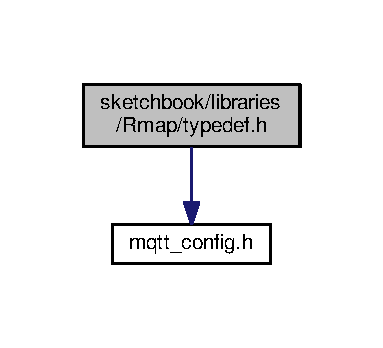
\includegraphics[width=184pt]{typedef_8h__incl}
\end{center}
\end{figure}
This graph shows which files directly or indirectly include this file\+:\nopagebreak
\begin{figure}[H]
\begin{center}
\leavevmode
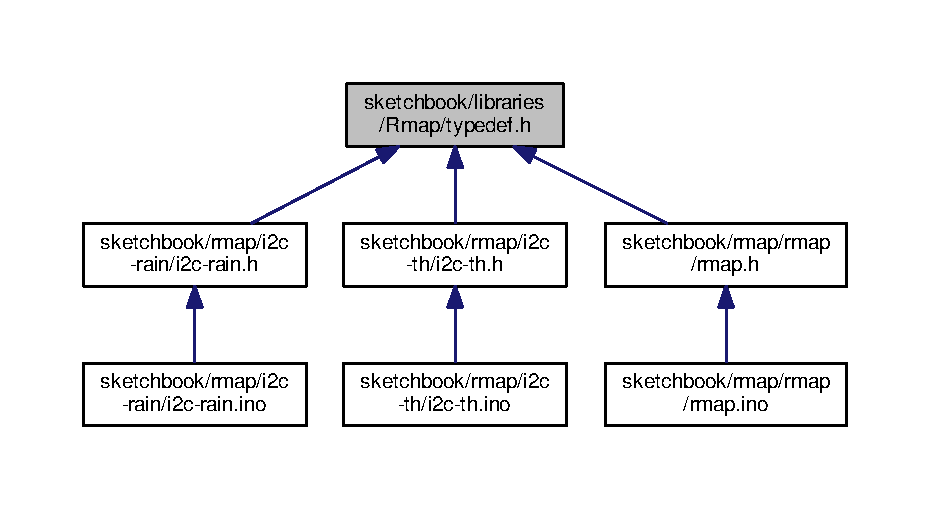
\includegraphics[width=350pt]{typedef_8h__dep__incl}
\end{center}
\end{figure}
\subsection*{Classes}
\begin{DoxyCompactItemize}
\item 
struct \hyperlink{structsensor__t}{sensor\+\_\+t}
\begin{DoxyCompactList}\small\item\em Sensor struct for storing sensor configuration parameter. \end{DoxyCompactList}\item 
struct \hyperlink{structrain__t}{rain\+\_\+t}
\begin{DoxyCompactList}\small\item\em Rain tips struct for storing rain tips count. \end{DoxyCompactList}\item 
struct \hyperlink{structvalue__t}{value\+\_\+t}
\begin{DoxyCompactList}\small\item\em Value struct for storing sample, observation and minium, average and maximum measurement. \end{DoxyCompactList}\end{DoxyCompactItemize}
\subsection*{Macros}
\begin{DoxyCompactItemize}
\item 
\mbox{\Hypertarget{typedef_8h_a343127490097a8ef68ab7d577d01b38b}\label{typedef_8h_a343127490097a8ef68ab7d577d01b38b}} 
\#define \hyperlink{typedef_8h_a343127490097a8ef68ab7d577d01b38b}{D\+R\+I\+V\+E\+R\+\_\+\+L\+E\+N\+G\+TH}~(5)
\begin{DoxyCompactList}\small\item\em Sensor driver\textquotesingle{}s buffer length. \end{DoxyCompactList}\item 
\mbox{\Hypertarget{typedef_8h_a7be6924e0d85f3f82149ea31cca36887}\label{typedef_8h_a7be6924e0d85f3f82149ea31cca36887}} 
\#define \hyperlink{typedef_8h_a7be6924e0d85f3f82149ea31cca36887}{T\+Y\+P\+E\+\_\+\+L\+E\+N\+G\+TH}~(5)
\begin{DoxyCompactList}\small\item\em Sensor type\textquotesingle{}s buffer length. \end{DoxyCompactList}\end{DoxyCompactItemize}

\hypertarget{debug__config_8h}{}\section{sketchbook/libraries/\+Rmap\+Config/debug\+\_\+config.h File Reference}
\label{debug__config_8h}\index{sketchbook/libraries/\+Rmap\+Config/debug\+\_\+config.\+h@{sketchbook/libraries/\+Rmap\+Config/debug\+\_\+config.\+h}}
This graph shows which files directly or indirectly include this file\+:\nopagebreak
\begin{figure}[H]
\begin{center}
\leavevmode
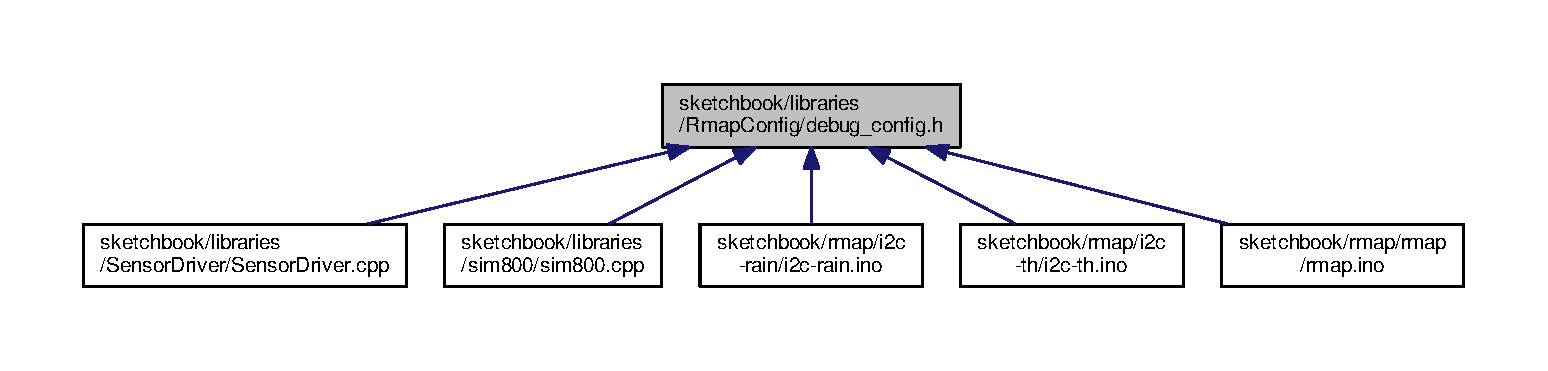
\includegraphics[width=350pt]{debug__config_8h__dep__incl}
\end{center}
\end{figure}
\subsection*{Macros}
\begin{DoxyCompactItemize}
\item 
\mbox{\Hypertarget{debug__config_8h_ab6322e7dccbadeed1a84b6e4b5eba819}\label{debug__config_8h_ab6322e7dccbadeed1a84b6e4b5eba819}} 
\#define \hyperlink{debug__config_8h_ab6322e7dccbadeed1a84b6e4b5eba819}{S\+E\+R\+I\+A\+L\+\_\+\+T\+R\+A\+C\+E\+\_\+\+L\+E\+V\+E\+L\+\_\+\+O\+FF}~(0)
\begin{DoxyCompactList}\small\item\em Debug level for disable debug on serial interface. \end{DoxyCompactList}\item 
\mbox{\Hypertarget{debug__config_8h_a3d7d4bfcbd372fce76d370f98a3a4402}\label{debug__config_8h_a3d7d4bfcbd372fce76d370f98a3a4402}} 
\#define \hyperlink{debug__config_8h_a3d7d4bfcbd372fce76d370f98a3a4402}{S\+E\+R\+I\+A\+L\+\_\+\+T\+R\+A\+C\+E\+\_\+\+L\+E\+V\+E\+L\+\_\+\+E\+R\+R\+OR}~(1)
\begin{DoxyCompactList}\small\item\em Debug level for print error message on serial interface. \end{DoxyCompactList}\item 
\mbox{\Hypertarget{debug__config_8h_adb8f42e979f3e8da9aac7a2d9b2a5ef5}\label{debug__config_8h_adb8f42e979f3e8da9aac7a2d9b2a5ef5}} 
\#define \hyperlink{debug__config_8h_adb8f42e979f3e8da9aac7a2d9b2a5ef5}{S\+E\+R\+I\+A\+L\+\_\+\+T\+R\+A\+C\+E\+\_\+\+L\+E\+V\+E\+L\+\_\+\+W\+A\+R\+N\+I\+NG}~(2)
\begin{DoxyCompactList}\small\item\em Debug level for print warning message on serial interface. \end{DoxyCompactList}\item 
\mbox{\Hypertarget{debug__config_8h_aa20d04ec16460dd4a377000a51f2406e}\label{debug__config_8h_aa20d04ec16460dd4a377000a51f2406e}} 
\#define \hyperlink{debug__config_8h_aa20d04ec16460dd4a377000a51f2406e}{S\+E\+R\+I\+A\+L\+\_\+\+T\+R\+A\+C\+E\+\_\+\+L\+E\+V\+E\+L\+\_\+\+I\+N\+FO}~(3)
\begin{DoxyCompactList}\small\item\em Debug level for print informations message on serial interface. \end{DoxyCompactList}\item 
\mbox{\Hypertarget{debug__config_8h_a3da5b046046a0d8e7aaefc07d8bc8e6b}\label{debug__config_8h_a3da5b046046a0d8e7aaefc07d8bc8e6b}} 
\#define \hyperlink{debug__config_8h_a3da5b046046a0d8e7aaefc07d8bc8e6b}{S\+E\+R\+I\+A\+L\+\_\+\+T\+R\+A\+C\+E\+\_\+\+L\+E\+V\+E\+L\+\_\+\+D\+E\+B\+UG}~(4)
\begin{DoxyCompactList}\small\item\em Debug level for print verbose informations message on serial interface. \end{DoxyCompactList}\item 
\mbox{\Hypertarget{debug__config_8h_ac23b745fd757e02c11f06e56791bcf6e}\label{debug__config_8h_ac23b745fd757e02c11f06e56791bcf6e}} 
\#define \hyperlink{debug__config_8h_ac23b745fd757e02c11f06e56791bcf6e}{S\+E\+R\+I\+A\+L\+\_\+\+T\+R\+A\+C\+E\+\_\+\+L\+E\+V\+E\+L\+\_\+\+T\+R\+A\+CE}~(5)
\begin{DoxyCompactList}\small\item\em Debug level for print detailed informations message on serial interface. \end{DoxyCompactList}\item 
\mbox{\Hypertarget{debug__config_8h_ab40fd4608517cbf6acb6d6d369f43253}\label{debug__config_8h_ab40fd4608517cbf6acb6d6d369f43253}} 
\#define \hyperlink{debug__config_8h_ab40fd4608517cbf6acb6d6d369f43253}{L\+C\+D\+\_\+\+T\+R\+A\+C\+E\+\_\+\+L\+E\+V\+E\+L\+\_\+\+O\+FF}~(0)
\begin{DoxyCompactList}\small\item\em Debug level for print error message on lcd interface. \end{DoxyCompactList}\item 
\mbox{\Hypertarget{debug__config_8h_a94e9ef9bebfaf0468a3165bd3499ce2a}\label{debug__config_8h_a94e9ef9bebfaf0468a3165bd3499ce2a}} 
\#define \hyperlink{debug__config_8h_a94e9ef9bebfaf0468a3165bd3499ce2a}{L\+C\+D\+\_\+\+T\+R\+A\+C\+E\+\_\+\+L\+E\+V\+E\+L\+\_\+\+E\+R\+R\+OR}~(1)
\begin{DoxyCompactList}\small\item\em Debug level for print error message on lcd. \end{DoxyCompactList}\item 
\mbox{\Hypertarget{debug__config_8h_a5df6cfd68b19362cf114761ca979fa7f}\label{debug__config_8h_a5df6cfd68b19362cf114761ca979fa7f}} 
\#define \hyperlink{debug__config_8h_a5df6cfd68b19362cf114761ca979fa7f}{L\+C\+D\+\_\+\+T\+R\+A\+C\+E\+\_\+\+L\+E\+V\+E\+L\+\_\+\+W\+A\+R\+N\+I\+NG}~(2)
\begin{DoxyCompactList}\small\item\em Debug level for print detailed informations message on serial interface. \end{DoxyCompactList}\item 
\mbox{\Hypertarget{debug__config_8h_a504c0d916f441917c6c0fd5638793e06}\label{debug__config_8h_a504c0d916f441917c6c0fd5638793e06}} 
\#define \hyperlink{debug__config_8h_a504c0d916f441917c6c0fd5638793e06}{L\+C\+D\+\_\+\+T\+R\+A\+C\+E\+\_\+\+L\+E\+V\+E\+L\+\_\+\+I\+N\+FO}~(3)
\begin{DoxyCompactList}\small\item\em Debug level for print informations message on lcd. \end{DoxyCompactList}\item 
\mbox{\Hypertarget{debug__config_8h_a32de94004e4a5148cd74f43133698e75}\label{debug__config_8h_a32de94004e4a5148cd74f43133698e75}} 
\#define \hyperlink{debug__config_8h_a32de94004e4a5148cd74f43133698e75}{L\+C\+D\+\_\+\+T\+R\+A\+C\+E\+\_\+\+L\+E\+V\+E\+L\+\_\+\+D\+E\+B\+UG}~(4)
\begin{DoxyCompactList}\small\item\em Debug level for print verbose informations message on lcd. \end{DoxyCompactList}\item 
\mbox{\Hypertarget{debug__config_8h_ac43195a0ae9148cc77260cbed563bbe9}\label{debug__config_8h_ac43195a0ae9148cc77260cbed563bbe9}} 
\#define \hyperlink{debug__config_8h_ac43195a0ae9148cc77260cbed563bbe9}{O\+K\+\_\+\+S\+T\+R\+I\+NG}~(\char`\"{}OK\char`\"{})
\begin{DoxyCompactList}\small\item\em \char`\"{}\+O\+K\char`\"{} string message. \end{DoxyCompactList}\item 
\mbox{\Hypertarget{debug__config_8h_aafb785ddac3a16af13fc903fc54643e6}\label{debug__config_8h_aafb785ddac3a16af13fc903fc54643e6}} 
\#define \hyperlink{debug__config_8h_aafb785ddac3a16af13fc903fc54643e6}{E\+R\+R\+O\+R\+\_\+\+S\+T\+R\+I\+NG}~(\char`\"{}E\+R\+R\+OR\char`\"{})
\begin{DoxyCompactList}\small\item\em \char`\"{}\+E\+R\+R\+O\+R\char`\"{} string message. \end{DoxyCompactList}\item 
\mbox{\Hypertarget{debug__config_8h_ad33687e22fc3169994351a33cf406543}\label{debug__config_8h_ad33687e22fc3169994351a33cf406543}} 
\#define \hyperlink{debug__config_8h_ad33687e22fc3169994351a33cf406543}{F\+A\+I\+L\+\_\+\+S\+T\+R\+I\+NG}~(\char`\"{}F\+A\+IL\char`\"{})
\begin{DoxyCompactList}\small\item\em \char`\"{}\+F\+A\+I\+L\char`\"{} string message. \end{DoxyCompactList}\item 
\mbox{\Hypertarget{debug__config_8h_a3c501a66c0a800bddc27155daae1c30b}\label{debug__config_8h_a3c501a66c0a800bddc27155daae1c30b}} 
\#define \hyperlink{debug__config_8h_a3c501a66c0a800bddc27155daae1c30b}{Y\+E\+S\+\_\+\+S\+T\+R\+I\+NG}~(\char`\"{}Y\+ES\char`\"{})
\begin{DoxyCompactList}\small\item\em \char`\"{}\+Y\+E\+S\char`\"{} string message. \end{DoxyCompactList}\item 
\mbox{\Hypertarget{debug__config_8h_a8f45558d61bb57954afabc7cbce19c55}\label{debug__config_8h_a8f45558d61bb57954afabc7cbce19c55}} 
\#define \hyperlink{debug__config_8h_a8f45558d61bb57954afabc7cbce19c55}{N\+O\+\_\+\+S\+T\+R\+I\+NG}~(\char`\"{}NO\char`\"{})
\begin{DoxyCompactList}\small\item\em \char`\"{}\+N\+O\char`\"{} string message. \end{DoxyCompactList}\item 
\mbox{\Hypertarget{debug__config_8h_a3ecaa92b2d8a3c55362dc402d8b4c681}\label{debug__config_8h_a3ecaa92b2d8a3c55362dc402d8b4c681}} 
\#define \hyperlink{debug__config_8h_a3ecaa92b2d8a3c55362dc402d8b4c681}{O\+N\+\_\+\+S\+T\+R\+I\+NG}~(\char`\"{}ON\char`\"{})
\begin{DoxyCompactList}\small\item\em \char`\"{}\+O\+N\char`\"{} string message. \end{DoxyCompactList}\item 
\mbox{\Hypertarget{debug__config_8h_a5e771036352564ee46980bcc2611e193}\label{debug__config_8h_a5e771036352564ee46980bcc2611e193}} 
\#define \hyperlink{debug__config_8h_a5e771036352564ee46980bcc2611e193}{O\+F\+F\+\_\+\+S\+T\+R\+I\+NG}~(\char`\"{}O\+FF\char`\"{})
\begin{DoxyCompactList}\small\item\em \char`\"{}\+O\+F\+F\char`\"{} string message. \end{DoxyCompactList}\item 
\mbox{\Hypertarget{debug__config_8h_a2d91396a5eefb574ed65184458b089cb}\label{debug__config_8h_a2d91396a5eefb574ed65184458b089cb}} 
\#define \hyperlink{debug__config_8h_a2d91396a5eefb574ed65184458b089cb}{S\+A\+V\+E\+\_\+\+S\+T\+R\+I\+NG}~(\char`\"{}S\+A\+VE\char`\"{})
\begin{DoxyCompactList}\small\item\em \char`\"{}\+S\+A\+V\+E\char`\"{} string message. \end{DoxyCompactList}\item 
\mbox{\Hypertarget{debug__config_8h_a94cfa13ad63cfb5a454d6ca5f2394efd}\label{debug__config_8h_a94cfa13ad63cfb5a454d6ca5f2394efd}} 
\#define \hyperlink{debug__config_8h_a94cfa13ad63cfb5a454d6ca5f2394efd}{S\+E\+N\+S\+O\+R\+\_\+\+D\+R\+I\+V\+E\+R\+\_\+\+S\+E\+R\+I\+A\+L\+\_\+\+T\+R\+A\+C\+E\+\_\+\+L\+E\+V\+EL}~(\hyperlink{debug__config_8h_aa20d04ec16460dd4a377000a51f2406e}{S\+E\+R\+I\+A\+L\+\_\+\+T\+R\+A\+C\+E\+\_\+\+L\+E\+V\+E\+L\+\_\+\+I\+N\+FO})
\begin{DoxyCompactList}\small\item\em Serial trace level debug for \hyperlink{classSensorDriver}{Sensor\+Driver} library. \end{DoxyCompactList}\item 
\mbox{\Hypertarget{debug__config_8h_aec7138a27bd06bd7254d4f6028c9499a}\label{debug__config_8h_aec7138a27bd06bd7254d4f6028c9499a}} 
\#define \hyperlink{debug__config_8h_aec7138a27bd06bd7254d4f6028c9499a}{S\+I\+M800\+\_\+\+S\+E\+R\+I\+A\+L\+\_\+\+T\+R\+A\+C\+E\+\_\+\+L\+E\+V\+EL}~(\hyperlink{debug__config_8h_aa20d04ec16460dd4a377000a51f2406e}{S\+E\+R\+I\+A\+L\+\_\+\+T\+R\+A\+C\+E\+\_\+\+L\+E\+V\+E\+L\+\_\+\+I\+N\+FO})
\begin{DoxyCompactList}\small\item\em Serial trace level debug for Sim800 library. \end{DoxyCompactList}\item 
\mbox{\Hypertarget{debug__config_8h_a0138759b880270bd48d1f329c5c0af4d}\label{debug__config_8h_a0138759b880270bd48d1f329c5c0af4d}} 
\#define \hyperlink{debug__config_8h_a0138759b880270bd48d1f329c5c0af4d}{I2\+C\+\_\+\+T\+H\+\_\+\+S\+E\+R\+I\+A\+L\+\_\+\+T\+R\+A\+C\+E\+\_\+\+L\+E\+V\+EL}~(\hyperlink{debug__config_8h_aa20d04ec16460dd4a377000a51f2406e}{S\+E\+R\+I\+A\+L\+\_\+\+T\+R\+A\+C\+E\+\_\+\+L\+E\+V\+E\+L\+\_\+\+I\+N\+FO})
\begin{DoxyCompactList}\small\item\em Serial trace level debug for i2c-\/th sketch. \end{DoxyCompactList}\item 
\mbox{\Hypertarget{debug__config_8h_ad3ed083a5171e08bb1e3b04391228a4f}\label{debug__config_8h_ad3ed083a5171e08bb1e3b04391228a4f}} 
\#define \hyperlink{debug__config_8h_ad3ed083a5171e08bb1e3b04391228a4f}{I2\+C\+\_\+\+R\+A\+I\+N\+\_\+\+S\+E\+R\+I\+A\+L\+\_\+\+T\+R\+A\+C\+E\+\_\+\+L\+E\+V\+EL}~(\hyperlink{debug__config_8h_aa20d04ec16460dd4a377000a51f2406e}{S\+E\+R\+I\+A\+L\+\_\+\+T\+R\+A\+C\+E\+\_\+\+L\+E\+V\+E\+L\+\_\+\+I\+N\+FO})
\begin{DoxyCompactList}\small\item\em Serial trace level debug for i2c-\/rain sketch. \end{DoxyCompactList}\item 
\mbox{\Hypertarget{debug__config_8h_a911c268100400a6e1b419b0b79396e16}\label{debug__config_8h_a911c268100400a6e1b419b0b79396e16}} 
\#define \hyperlink{debug__config_8h_a911c268100400a6e1b419b0b79396e16}{R\+M\+A\+P\+\_\+\+S\+E\+R\+I\+A\+L\+\_\+\+T\+R\+A\+C\+E\+\_\+\+L\+E\+V\+EL}~(\hyperlink{debug__config_8h_aa20d04ec16460dd4a377000a51f2406e}{S\+E\+R\+I\+A\+L\+\_\+\+T\+R\+A\+C\+E\+\_\+\+L\+E\+V\+E\+L\+\_\+\+I\+N\+FO})
\begin{DoxyCompactList}\small\item\em Serial trace level debug for rmap sketch. \end{DoxyCompactList}\item 
\mbox{\Hypertarget{debug__config_8h_a86050508a20f5b64f14679edbc3640ab}\label{debug__config_8h_a86050508a20f5b64f14679edbc3640ab}} 
\#define \hyperlink{debug__config_8h_a86050508a20f5b64f14679edbc3640ab}{R\+M\+A\+P\+\_\+\+L\+C\+D\+\_\+\+T\+R\+A\+C\+E\+\_\+\+L\+E\+V\+EL}~(\hyperlink{debug__config_8h_a504c0d916f441917c6c0fd5638793e06}{L\+C\+D\+\_\+\+T\+R\+A\+C\+E\+\_\+\+L\+E\+V\+E\+L\+\_\+\+I\+N\+FO})
\begin{DoxyCompactList}\small\item\em Lcd trace level debug for rmap sketch. \end{DoxyCompactList}\end{DoxyCompactItemize}

\hypertarget{ethernet__config_8h}{}\section{sketchbook/libraries/\+Rmap\+Config/ethernet\+\_\+config.h File Reference}
\label{ethernet__config_8h}\index{sketchbook/libraries/\+Rmap\+Config/ethernet\+\_\+config.\+h@{sketchbook/libraries/\+Rmap\+Config/ethernet\+\_\+config.\+h}}
This graph shows which files directly or indirectly include this file\+:\nopagebreak
\begin{figure}[H]
\begin{center}
\leavevmode
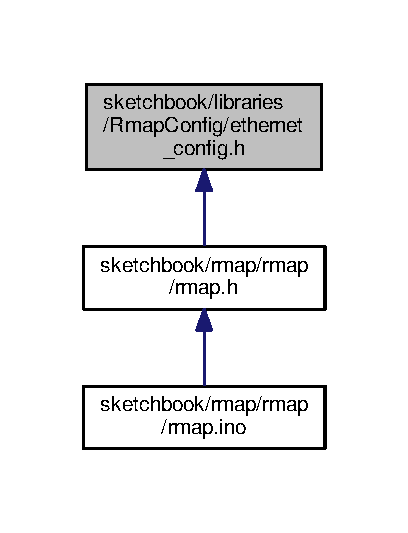
\includegraphics[width=196pt]{ethernet__config_8h__dep__incl}
\end{center}
\end{figure}
\subsection*{Macros}
\begin{DoxyCompactItemize}
\item 
\mbox{\Hypertarget{ethernet__config_8h_a6d72f280384bb90ffd7c78bb188dd6ad}\label{ethernet__config_8h_a6d72f280384bb90ffd7c78bb188dd6ad}} 
\#define \hyperlink{ethernet__config_8h_a6d72f280384bb90ffd7c78bb188dd6ad}{E\+T\+H\+E\+R\+N\+E\+T\+\_\+\+D\+E\+F\+A\+U\+L\+T\+\_\+\+D\+H\+C\+P\+\_\+\+E\+N\+A\+B\+LE}~(true)
\begin{DoxyCompactList}\small\item\em Default option for enable or disable D\+H\+CP protocol with ethernet. \end{DoxyCompactList}\item 
\mbox{\Hypertarget{ethernet__config_8h_aec01256edf75fe9fc49e47cd1e5954f6}\label{ethernet__config_8h_aec01256edf75fe9fc49e47cd1e5954f6}} 
\#define \hyperlink{ethernet__config_8h_aec01256edf75fe9fc49e47cd1e5954f6}{E\+T\+H\+E\+R\+N\+E\+T\+\_\+\+D\+E\+F\+A\+U\+L\+T\+\_\+\+M\+AC}~(\char`\"{}E2\+:21\+:\+B6\+:44\+:\+E\+B\+:29\char`\"{})
\begin{DoxyCompactList}\small\item\em Default mac address for ethernet device. \end{DoxyCompactList}\item 
\mbox{\Hypertarget{ethernet__config_8h_a708f80b356d050b3caada102553a6fb6}\label{ethernet__config_8h_a708f80b356d050b3caada102553a6fb6}} 
\#define \hyperlink{ethernet__config_8h_a708f80b356d050b3caada102553a6fb6}{E\+T\+H\+E\+R\+N\+E\+T\+\_\+\+D\+E\+F\+A\+U\+L\+T\+\_\+\+IP}~(\char`\"{}192.\+168.\+0.\+100\char`\"{})
\begin{DoxyCompactList}\small\item\em Default ip address for ethernet device. \end{DoxyCompactList}\item 
\mbox{\Hypertarget{ethernet__config_8h_a549e67e6695e819967dde18ea96f106d}\label{ethernet__config_8h_a549e67e6695e819967dde18ea96f106d}} 
\#define \hyperlink{ethernet__config_8h_a549e67e6695e819967dde18ea96f106d}{E\+T\+H\+E\+R\+N\+E\+T\+\_\+\+D\+E\+F\+A\+U\+L\+T\+\_\+\+N\+E\+T\+M\+A\+SK}~(\char`\"{}255.\+255.\+255.\+0\char`\"{})
\begin{DoxyCompactList}\small\item\em Default netmask for ethernet device. \end{DoxyCompactList}\item 
\mbox{\Hypertarget{ethernet__config_8h_a47956941b8ebab9ce04debc51848bfbd}\label{ethernet__config_8h_a47956941b8ebab9ce04debc51848bfbd}} 
\#define \hyperlink{ethernet__config_8h_a47956941b8ebab9ce04debc51848bfbd}{E\+T\+H\+E\+R\+N\+E\+T\+\_\+\+D\+E\+F\+A\+U\+L\+T\+\_\+\+G\+A\+T\+E\+W\+AY}~(\char`\"{}192.\+168.\+0.\+1\char`\"{})
\begin{DoxyCompactList}\small\item\em Default gateway for ethernet device. \end{DoxyCompactList}\item 
\mbox{\Hypertarget{ethernet__config_8h_ae21c97b50820450862c66c8d1d7f07e8}\label{ethernet__config_8h_ae21c97b50820450862c66c8d1d7f07e8}} 
\#define \hyperlink{ethernet__config_8h_ae21c97b50820450862c66c8d1d7f07e8}{E\+T\+H\+E\+R\+N\+E\+T\+\_\+\+D\+E\+F\+A\+U\+L\+T\+\_\+\+P\+R\+I\+M\+A\+R\+Y\+\_\+\+D\+NS}~(\char`\"{}192.\+168.\+0.\+1\char`\"{})
\begin{DoxyCompactList}\small\item\em Default primary dns for ethernet device. \end{DoxyCompactList}\item 
\mbox{\Hypertarget{ethernet__config_8h_a4e199cc3c1e424cd0e704d1ab28dda4f}\label{ethernet__config_8h_a4e199cc3c1e424cd0e704d1ab28dda4f}} 
\#define \hyperlink{ethernet__config_8h_a4e199cc3c1e424cd0e704d1ab28dda4f}{E\+T\+H\+E\+R\+N\+E\+T\+\_\+\+D\+E\+F\+A\+U\+L\+T\+\_\+\+L\+O\+C\+A\+L\+\_\+\+U\+D\+P\+\_\+\+P\+O\+RT}~(8000)
\begin{DoxyCompactList}\small\item\em Default local udp port for ethernet device. \end{DoxyCompactList}\item 
\mbox{\Hypertarget{ethernet__config_8h_a33ddf6002b3cabe6872997f10ce52a3b}\label{ethernet__config_8h_a33ddf6002b3cabe6872997f10ce52a3b}} 
\#define \hyperlink{ethernet__config_8h_a33ddf6002b3cabe6872997f10ce52a3b}{E\+T\+H\+E\+R\+N\+E\+T\+\_\+\+A\+T\+T\+E\+M\+P\+T\+\_\+\+MS}~(2000)
\begin{DoxyCompactList}\small\item\em Set next ethernet library attempt delay in milliseconds after a failure. \end{DoxyCompactList}\item 
\mbox{\Hypertarget{ethernet__config_8h_ad03ea08cdc08494fd3562b76c3e6faf4}\label{ethernet__config_8h_ad03ea08cdc08494fd3562b76c3e6faf4}} 
\#define \hyperlink{ethernet__config_8h_ad03ea08cdc08494fd3562b76c3e6faf4}{E\+T\+H\+E\+R\+N\+E\+T\+\_\+\+R\+E\+T\+R\+Y\+\_\+\+T\+I\+M\+E\+\_\+\+MS}~(4000)
\begin{DoxyCompactList}\small\item\em Set next ethernet task attempt delay in milliseconds after a failure. \end{DoxyCompactList}\item 
\mbox{\Hypertarget{ethernet__config_8h_a474986eade043f4b67c86a16aeddd81b}\label{ethernet__config_8h_a474986eade043f4b67c86a16aeddd81b}} 
\#define \hyperlink{ethernet__config_8h_a474986eade043f4b67c86a16aeddd81b}{E\+T\+H\+E\+R\+N\+E\+T\+\_\+\+R\+E\+T\+R\+Y\+\_\+\+C\+O\+U\+NT}~(3)
\begin{DoxyCompactList}\small\item\em Maximum number of retry for ethernet task. \end{DoxyCompactList}\item 
\mbox{\Hypertarget{ethernet__config_8h_a17b3b46c88879aaf5fd4e663e073f731}\label{ethernet__config_8h_a17b3b46c88879aaf5fd4e663e073f731}} 
\#define \hyperlink{ethernet__config_8h_a17b3b46c88879aaf5fd4e663e073f731}{E\+T\+H\+E\+R\+N\+E\+T\+\_\+\+M\+Q\+T\+T\+\_\+\+T\+I\+M\+E\+O\+U\+T\+\_\+\+MS}~(6000)
\begin{DoxyCompactList}\small\item\em M\+Q\+TT timeout in milliseconds for ethernet device. \end{DoxyCompactList}\item 
\mbox{\Hypertarget{ethernet__config_8h_aafad911924144dbfc03b66b146ed4439}\label{ethernet__config_8h_aafad911924144dbfc03b66b146ed4439}} 
\#define \hyperlink{ethernet__config_8h_aafad911924144dbfc03b66b146ed4439}{E\+T\+H\+E\+R\+N\+E\+T\+\_\+\+M\+A\+C\+\_\+\+L\+E\+N\+G\+TH}~(6)
\begin{DoxyCompactList}\small\item\em Length in bytes for mac address. \end{DoxyCompactList}\item 
\mbox{\Hypertarget{ethernet__config_8h_ae8de53528e88d8ff4516d82a48590bd7}\label{ethernet__config_8h_ae8de53528e88d8ff4516d82a48590bd7}} 
\#define \hyperlink{ethernet__config_8h_ae8de53528e88d8ff4516d82a48590bd7}{E\+T\+H\+E\+R\+N\+E\+T\+\_\+\+I\+P\+\_\+\+L\+E\+N\+G\+TH}~(4)
\begin{DoxyCompactList}\small\item\em Length in bytes for ip address. \end{DoxyCompactList}\end{DoxyCompactItemize}

\hypertarget{gsm__config_8h}{}\section{sketchbook/libraries/\+Rmap\+Config/gsm\+\_\+config.h File Reference}
\label{gsm__config_8h}\index{sketchbook/libraries/\+Rmap\+Config/gsm\+\_\+config.\+h@{sketchbook/libraries/\+Rmap\+Config/gsm\+\_\+config.\+h}}
\subsection*{Macros}
\begin{DoxyCompactItemize}
\item 
\mbox{\Hypertarget{gsm__config_8h_a876e54d28d81219bdc35336ddbbcbab7}\label{gsm__config_8h_a876e54d28d81219bdc35336ddbbcbab7}} 
\#define \hyperlink{gsm__config_8h_a876e54d28d81219bdc35336ddbbcbab7}{G\+S\+M\+\_\+\+A\+P\+N\+\_\+\+T\+IM}~(\char`\"{}ibox.\+tim.\+it\char`\"{})
\begin{DoxyCompactList}\small\item\em A\+PN for T\+IM. \end{DoxyCompactList}\item 
\mbox{\Hypertarget{gsm__config_8h_a97ae5024ec54ae476fc14842464054c5}\label{gsm__config_8h_a97ae5024ec54ae476fc14842464054c5}} 
\#define \hyperlink{gsm__config_8h_a97ae5024ec54ae476fc14842464054c5}{G\+S\+M\+\_\+\+A\+P\+N\+\_\+\+W\+I\+ND}~(\char`\"{}internet.\+wind\char`\"{})
\begin{DoxyCompactList}\small\item\em A\+PN for W\+I\+ND. \end{DoxyCompactList}\item 
\mbox{\Hypertarget{gsm__config_8h_abe5d352358080d78516aa1e7643161f5}\label{gsm__config_8h_abe5d352358080d78516aa1e7643161f5}} 
\#define \hyperlink{gsm__config_8h_abe5d352358080d78516aa1e7643161f5}{G\+S\+M\+\_\+\+A\+P\+N\+\_\+\+V\+O\+D\+A\+F\+O\+NE}~(\char`\"{}web.\+omnitel.\+it\char`\"{})
\begin{DoxyCompactList}\small\item\em A\+PN for V\+O\+D\+A\+F\+O\+NE. \end{DoxyCompactList}\item 
\mbox{\Hypertarget{gsm__config_8h_a1697d2d335c6f12c9a1b3139e364c377}\label{gsm__config_8h_a1697d2d335c6f12c9a1b3139e364c377}} 
\#define \hyperlink{gsm__config_8h_a1697d2d335c6f12c9a1b3139e364c377}{G\+S\+M\+\_\+\+D\+E\+F\+A\+U\+L\+T\+\_\+\+A\+PN}~(\hyperlink{gsm__config_8h_abe5d352358080d78516aa1e7643161f5}{G\+S\+M\+\_\+\+A\+P\+N\+\_\+\+V\+O\+D\+A\+F\+O\+NE})
\begin{DoxyCompactList}\small\item\em Default G\+SM A\+PN. \end{DoxyCompactList}\item 
\mbox{\Hypertarget{gsm__config_8h_aa00383ae345a8a8646d5aec400923a75}\label{gsm__config_8h_aa00383ae345a8a8646d5aec400923a75}} 
\#define \hyperlink{gsm__config_8h_aa00383ae345a8a8646d5aec400923a75}{G\+S\+M\+\_\+\+D\+E\+F\+A\+U\+L\+T\+\_\+\+U\+S\+E\+R\+N\+A\+ME}~(\char`\"{}\char`\"{})
\begin{DoxyCompactList}\small\item\em Default G\+SM username. \end{DoxyCompactList}\item 
\mbox{\Hypertarget{gsm__config_8h_a0095817f909014a0e961904f3c6b9df0}\label{gsm__config_8h_a0095817f909014a0e961904f3c6b9df0}} 
\#define \hyperlink{gsm__config_8h_a0095817f909014a0e961904f3c6b9df0}{G\+S\+M\+\_\+\+D\+E\+F\+A\+U\+L\+T\+\_\+\+P\+A\+S\+S\+W\+O\+RD}~(\char`\"{}\char`\"{})
\begin{DoxyCompactList}\small\item\em Default G\+SM password. \end{DoxyCompactList}\item 
\mbox{\Hypertarget{gsm__config_8h_a79742432357daf12af51d24f3ad49181}\label{gsm__config_8h_a79742432357daf12af51d24f3ad49181}} 
\#define \hyperlink{gsm__config_8h_a79742432357daf12af51d24f3ad49181}{G\+S\+M\+\_\+\+A\+P\+N\+\_\+\+L\+E\+N\+G\+TH}~(20)
\begin{DoxyCompactList}\small\item\em Length in bytes for apn. \end{DoxyCompactList}\item 
\mbox{\Hypertarget{gsm__config_8h_a4283edb5b450bf98e2a7f8cc20c762af}\label{gsm__config_8h_a4283edb5b450bf98e2a7f8cc20c762af}} 
\#define \hyperlink{gsm__config_8h_a4283edb5b450bf98e2a7f8cc20c762af}{G\+S\+M\+\_\+\+U\+S\+E\+R\+N\+A\+M\+E\+\_\+\+L\+E\+N\+G\+TH}~(20)
\begin{DoxyCompactList}\small\item\em Length in bytes for username. \end{DoxyCompactList}\item 
\mbox{\Hypertarget{gsm__config_8h_a668cdca5d1371199acbf4b15f8e897f7}\label{gsm__config_8h_a668cdca5d1371199acbf4b15f8e897f7}} 
\#define \hyperlink{gsm__config_8h_a668cdca5d1371199acbf4b15f8e897f7}{G\+S\+M\+\_\+\+P\+A\+S\+S\+W\+O\+R\+D\+\_\+\+L\+E\+N\+G\+TH}~(20)
\begin{DoxyCompactList}\small\item\em Length in bytes for password. \end{DoxyCompactList}\item 
\mbox{\Hypertarget{gsm__config_8h_ac4bfe5ea70a0f723e2925838b7b52b8a}\label{gsm__config_8h_ac4bfe5ea70a0f723e2925838b7b52b8a}} 
\#define \hyperlink{gsm__config_8h_ac4bfe5ea70a0f723e2925838b7b52b8a}{U\+S\+E\+\_\+\+S\+I\+M\+\_\+800C}~(true)
\begin{DoxyCompactList}\small\item\em Enable if you want to use S\+I\+M800C. \end{DoxyCompactList}\item 
\mbox{\Hypertarget{gsm__config_8h_a786ce1985a009e8c8faf75435df54842}\label{gsm__config_8h_a786ce1985a009e8c8faf75435df54842}} 
\#define \hyperlink{gsm__config_8h_a786ce1985a009e8c8faf75435df54842}{U\+S\+E\+\_\+\+S\+I\+M\+\_\+800L}~(false)
\begin{DoxyCompactList}\small\item\em Enable if you want to use S\+I\+M800L. \end{DoxyCompactList}\end{DoxyCompactItemize}

\hypertarget{hardware__config_8h}{}\section{sketchbook/libraries/\+Rmap\+Config/hardware\+\_\+config.h File Reference}
\label{hardware__config_8h}\index{sketchbook/libraries/\+Rmap\+Config/hardware\+\_\+config.\+h@{sketchbook/libraries/\+Rmap\+Config/hardware\+\_\+config.\+h}}
This graph shows which files directly or indirectly include this file\+:\nopagebreak
\begin{figure}[H]
\begin{center}
\leavevmode
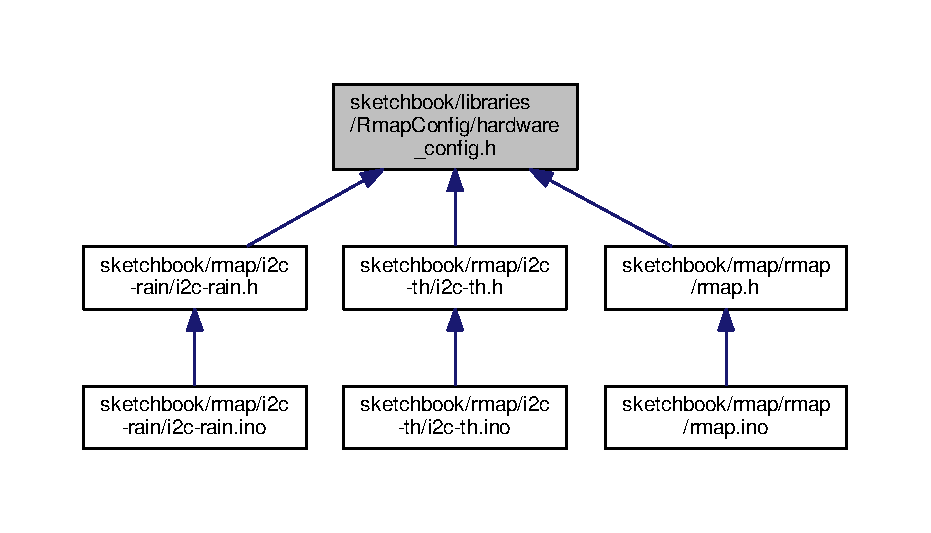
\includegraphics[width=350pt]{hardware__config_8h__dep__incl}
\end{center}
\end{figure}
\subsection*{Macros}
\begin{DoxyCompactItemize}
\item 
\mbox{\Hypertarget{hardware__config_8h_a0375e429bddace9b0ff67efc738aa314}\label{hardware__config_8h_a0375e429bddace9b0ff67efc738aa314}} 
\#define \hyperlink{hardware__config_8h_a0375e429bddace9b0ff67efc738aa314}{I2\+C\+\_\+\+B\+U\+S\+\_\+\+C\+L\+O\+CK}~(50000\+L)
\begin{DoxyCompactList}\small\item\em I2C bus clock in Hertz. \end{DoxyCompactList}\item 
\mbox{\Hypertarget{hardware__config_8h_aa552d72ce15dd8ca167c4b9323f1f25d}\label{hardware__config_8h_aa552d72ce15dd8ca167c4b9323f1f25d}} 
\#define \hyperlink{hardware__config_8h_aa552d72ce15dd8ca167c4b9323f1f25d}{I2\+C\+\_\+\+M\+A\+X\+\_\+\+D\+A\+T\+A\+\_\+\+L\+E\+N\+G\+TH}~(32)
\begin{DoxyCompactList}\small\item\em Max length in bytes for i2c bus data buffer. \end{DoxyCompactList}\end{DoxyCompactItemize}

\hypertarget{json__config_8h}{}\section{sketchbook/libraries/\+Rmap\+Config/json\+\_\+config.h File Reference}
\label{json__config_8h}\index{sketchbook/libraries/\+Rmap\+Config/json\+\_\+config.\+h@{sketchbook/libraries/\+Rmap\+Config/json\+\_\+config.\+h}}
This graph shows which files directly or indirectly include this file\+:\nopagebreak
\begin{figure}[H]
\begin{center}
\leavevmode
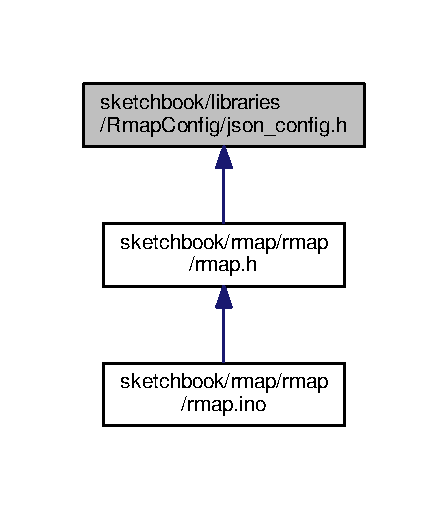
\includegraphics[width=215pt]{json__config_8h__dep__incl}
\end{center}
\end{figure}
\subsection*{Macros}
\begin{DoxyCompactItemize}
\item 
\mbox{\Hypertarget{json__config_8h_a0a84205906d82fe38eb136a6384fd1c8}\label{json__config_8h_a0a84205906d82fe38eb136a6384fd1c8}} 
\#define \hyperlink{json__config_8h_a0a84205906d82fe38eb136a6384fd1c8}{J\+S\+O\+N\+\_\+\+B\+U\+F\+F\+E\+R\+\_\+\+L\+E\+N\+G\+TH}~(70)
\begin{DoxyCompactList}\small\item\em Length in bytes for J\+S\+ON data buffer. \end{DoxyCompactList}\end{DoxyCompactItemize}

\hypertarget{lcd__config_8h}{}\section{sketchbook/libraries/\+Rmap\+Config/lcd\+\_\+config.h File Reference}
\label{lcd__config_8h}\index{sketchbook/libraries/\+Rmap\+Config/lcd\+\_\+config.\+h@{sketchbook/libraries/\+Rmap\+Config/lcd\+\_\+config.\+h}}
This graph shows which files directly or indirectly include this file\+:\nopagebreak
\begin{figure}[H]
\begin{center}
\leavevmode
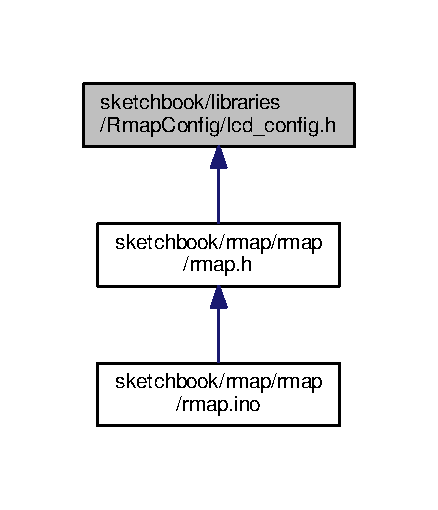
\includegraphics[width=210pt]{lcd__config_8h__dep__incl}
\end{center}
\end{figure}
\subsection*{Macros}
\begin{DoxyCompactItemize}
\item 
\mbox{\Hypertarget{lcd__config_8h_aabe3eae58b7e15bab0e4e34245079410}\label{lcd__config_8h_aabe3eae58b7e15bab0e4e34245079410}} 
\#define \hyperlink{lcd__config_8h_aabe3eae58b7e15bab0e4e34245079410}{L\+C\+D\+\_\+\+I2\+C\+\_\+\+A\+D\+D\+R\+E\+SS}~(0x3\+F)
\begin{DoxyCompactList}\small\item\em Default L\+CD i2c address. \end{DoxyCompactList}\item 
\mbox{\Hypertarget{lcd__config_8h_a537e0d54d9ec6c708bd8990c2f4d8e64}\label{lcd__config_8h_a537e0d54d9ec6c708bd8990c2f4d8e64}} 
\#define \hyperlink{lcd__config_8h_a537e0d54d9ec6c708bd8990c2f4d8e64}{L\+C\+D\+\_\+\+C\+O\+L\+U\+M\+NS}~(20)
\begin{DoxyCompactList}\small\item\em Default L\+CD columns number. \end{DoxyCompactList}\item 
\mbox{\Hypertarget{lcd__config_8h_a9a59fc4d524d3519a6bd0cb451850a65}\label{lcd__config_8h_a9a59fc4d524d3519a6bd0cb451850a65}} 
\#define \hyperlink{lcd__config_8h_a9a59fc4d524d3519a6bd0cb451850a65}{L\+C\+D\+\_\+\+R\+O\+WS}~(4)
\begin{DoxyCompactList}\small\item\em Default L\+CD rows number. \end{DoxyCompactList}\end{DoxyCompactItemize}

\hypertarget{mqtt__config_8h}{}\section{sketchbook/libraries/\+Rmap\+Config/mqtt\+\_\+config.h File Reference}
\label{mqtt__config_8h}\index{sketchbook/libraries/\+Rmap\+Config/mqtt\+\_\+config.\+h@{sketchbook/libraries/\+Rmap\+Config/mqtt\+\_\+config.\+h}}
This graph shows which files directly or indirectly include this file\+:\nopagebreak
\begin{figure}[H]
\begin{center}
\leavevmode
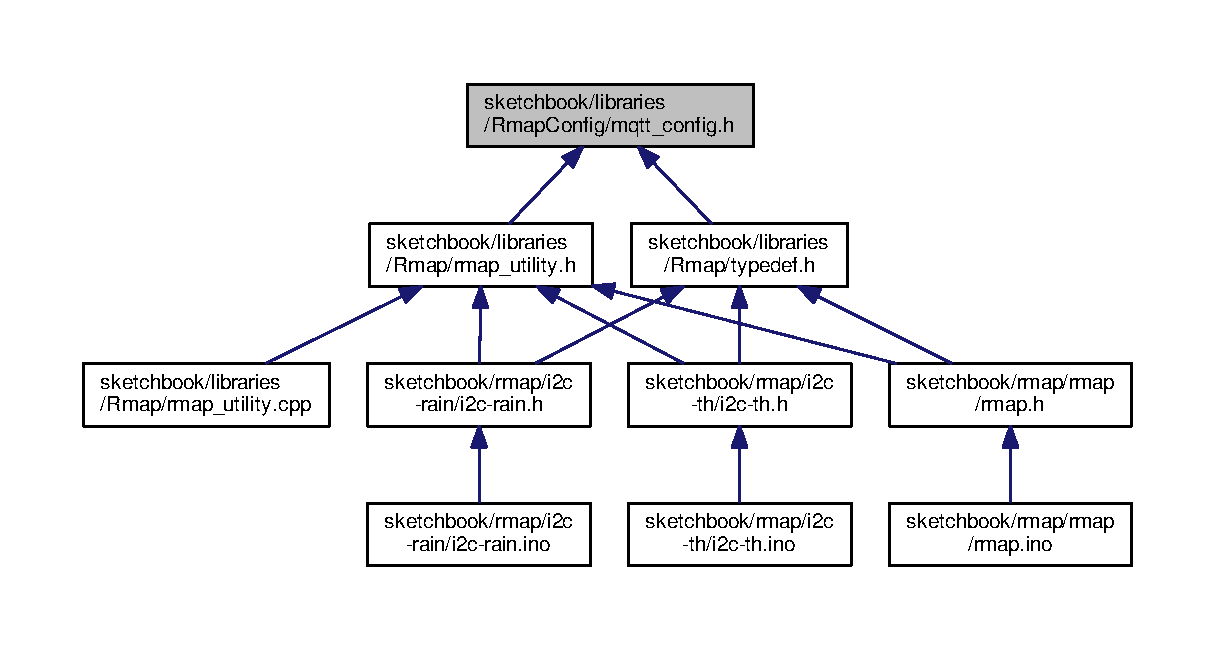
\includegraphics[width=350pt]{mqtt__config_8h__dep__incl}
\end{center}
\end{figure}
\subsection*{Macros}
\begin{DoxyCompactItemize}
\item 
\mbox{\Hypertarget{mqtt__config_8h_a6d3b5b0f9c41b605e608f7d460491be6}\label{mqtt__config_8h_a6d3b5b0f9c41b605e608f7d460491be6}} 
\#define \hyperlink{mqtt__config_8h_a6d3b5b0f9c41b605e608f7d460491be6}{M\+Q\+T\+T\+\_\+\+R\+O\+O\+T\+\_\+\+T\+O\+P\+I\+C\+\_\+\+L\+E\+N\+G\+TH}~(50)
\begin{DoxyCompactList}\small\item\em Length in bytes for mqtt root topic. \end{DoxyCompactList}\item 
\mbox{\Hypertarget{mqtt__config_8h_a5be9d9eee2bf528b0fd12a0bda5c246a}\label{mqtt__config_8h_a5be9d9eee2bf528b0fd12a0bda5c246a}} 
\#define \hyperlink{mqtt__config_8h_a5be9d9eee2bf528b0fd12a0bda5c246a}{M\+Q\+T\+T\+\_\+\+M\+A\+I\+N\+T\+\_\+\+T\+O\+P\+I\+C\+\_\+\+L\+E\+N\+G\+TH}~(\hyperlink{mqtt__config_8h_a6d3b5b0f9c41b605e608f7d460491be6}{M\+Q\+T\+T\+\_\+\+R\+O\+O\+T\+\_\+\+T\+O\+P\+I\+C\+\_\+\+L\+E\+N\+G\+TH})
\begin{DoxyCompactList}\small\item\em Length in bytes for mqtt maint topic. \end{DoxyCompactList}\item 
\mbox{\Hypertarget{mqtt__config_8h_a2517f6560f7ee99813533e63d7fc91b6}\label{mqtt__config_8h_a2517f6560f7ee99813533e63d7fc91b6}} 
\#define \hyperlink{mqtt__config_8h_a2517f6560f7ee99813533e63d7fc91b6}{M\+Q\+T\+T\+\_\+\+S\+U\+B\+S\+C\+R\+I\+B\+E\+\_\+\+T\+O\+P\+I\+C\+\_\+\+L\+E\+N\+G\+TH}~(50)
\begin{DoxyCompactList}\small\item\em Length in bytes for mqtt subscibe topic. \end{DoxyCompactList}\item 
\mbox{\Hypertarget{mqtt__config_8h_a85772fcdfe85fa51f02f3045c0aa7764}\label{mqtt__config_8h_a85772fcdfe85fa51f02f3045c0aa7764}} 
\#define \hyperlink{mqtt__config_8h_a85772fcdfe85fa51f02f3045c0aa7764}{M\+Q\+T\+T\+\_\+\+S\+E\+N\+S\+O\+R\+\_\+\+T\+O\+P\+I\+C\+\_\+\+L\+E\+N\+G\+TH}~(30)
\begin{DoxyCompactList}\small\item\em Length in bytes for mqtt sensor topic. \end{DoxyCompactList}\item 
\mbox{\Hypertarget{mqtt__config_8h_a16c3df993e6090c9e607113aaf5421f6}\label{mqtt__config_8h_a16c3df993e6090c9e607113aaf5421f6}} 
\#define \hyperlink{mqtt__config_8h_a16c3df993e6090c9e607113aaf5421f6}{M\+Q\+T\+T\+\_\+\+C\+L\+I\+E\+N\+T\+\_\+\+I\+D\+\_\+\+L\+E\+N\+G\+TH}~(\hyperlink{mqtt__config_8h_a6d3b5b0f9c41b605e608f7d460491be6}{M\+Q\+T\+T\+\_\+\+R\+O\+O\+T\+\_\+\+T\+O\+P\+I\+C\+\_\+\+L\+E\+N\+G\+TH})
\begin{DoxyCompactList}\small\item\em Length in bytes for mqtt client id. \end{DoxyCompactList}\item 
\mbox{\Hypertarget{mqtt__config_8h_a0fff77926fd907aeb2c03f60600d136c}\label{mqtt__config_8h_a0fff77926fd907aeb2c03f60600d136c}} 
\#define \hyperlink{mqtt__config_8h_a0fff77926fd907aeb2c03f60600d136c}{M\+Q\+T\+T\+\_\+\+M\+E\+S\+S\+A\+G\+E\+\_\+\+L\+E\+N\+G\+TH}~(50)
\begin{DoxyCompactList}\small\item\em Length in bytes for mqtt message. \end{DoxyCompactList}\item 
\mbox{\Hypertarget{mqtt__config_8h_a0a37bcf35cdbfc63d72beca198759c08}\label{mqtt__config_8h_a0a37bcf35cdbfc63d72beca198759c08}} 
\#define \hyperlink{mqtt__config_8h_a0a37bcf35cdbfc63d72beca198759c08}{M\+Q\+T\+T\+\_\+\+S\+E\+R\+V\+E\+R\+\_\+\+L\+E\+N\+G\+TH}~(30)
\begin{DoxyCompactList}\small\item\em Length in bytes for mqtt server. \end{DoxyCompactList}\item 
\mbox{\Hypertarget{mqtt__config_8h_a0e1860b8d036f571ffcb7e6d27832c16}\label{mqtt__config_8h_a0e1860b8d036f571ffcb7e6d27832c16}} 
\#define \hyperlink{mqtt__config_8h_a0e1860b8d036f571ffcb7e6d27832c16}{M\+Q\+T\+T\+\_\+\+U\+S\+E\+R\+N\+A\+M\+E\+\_\+\+L\+E\+N\+G\+TH}~(30)
\begin{DoxyCompactList}\small\item\em Length in bytes for mqtt username. \end{DoxyCompactList}\item 
\mbox{\Hypertarget{mqtt__config_8h_a9fa040018ffd349e846cec27b2791fde}\label{mqtt__config_8h_a9fa040018ffd349e846cec27b2791fde}} 
\#define \hyperlink{mqtt__config_8h_a9fa040018ffd349e846cec27b2791fde}{M\+Q\+T\+T\+\_\+\+P\+A\+S\+S\+W\+O\+R\+D\+\_\+\+L\+E\+N\+G\+TH}~(30)
\begin{DoxyCompactList}\small\item\em Length in bytes for mqtt password. \end{DoxyCompactList}\item 
\mbox{\Hypertarget{mqtt__config_8h_abfcc7e625e42a553de9c3132faef282b}\label{mqtt__config_8h_abfcc7e625e42a553de9c3132faef282b}} 
\#define \hyperlink{mqtt__config_8h_abfcc7e625e42a553de9c3132faef282b}{M\+Q\+T\+T\+\_\+\+T\+I\+M\+E\+O\+U\+T\+\_\+\+MS}~(6000)
\begin{DoxyCompactList}\small\item\em Timeout in milliseconds for mqtt stack. \end{DoxyCompactList}\item 
\mbox{\Hypertarget{mqtt__config_8h_a509e4f28ec3987701a1c63c238b79716}\label{mqtt__config_8h_a509e4f28ec3987701a1c63c238b79716}} 
\#define \hyperlink{mqtt__config_8h_a509e4f28ec3987701a1c63c238b79716}{M\+Q\+T\+T\+\_\+\+D\+E\+F\+A\+U\+L\+T\+\_\+\+S\+E\+R\+V\+ER}~(\char`\"{}rmap.\+cc\char`\"{})
\begin{DoxyCompactList}\small\item\em Default M\+Q\+TT server. \end{DoxyCompactList}\item 
\mbox{\Hypertarget{mqtt__config_8h_a47dbba2fb767e8362864895e3ce87a36}\label{mqtt__config_8h_a47dbba2fb767e8362864895e3ce87a36}} 
\#define \hyperlink{mqtt__config_8h_a47dbba2fb767e8362864895e3ce87a36}{M\+Q\+T\+T\+\_\+\+D\+E\+F\+A\+U\+L\+T\+\_\+\+P\+O\+RT}~(1883)
\begin{DoxyCompactList}\small\item\em Default M\+Q\+TT server port. \end{DoxyCompactList}\item 
\mbox{\Hypertarget{mqtt__config_8h_a2b1941298e45ce3305da283122a525dc}\label{mqtt__config_8h_a2b1941298e45ce3305da283122a525dc}} 
\#define \hyperlink{mqtt__config_8h_a2b1941298e45ce3305da283122a525dc}{M\+Q\+T\+T\+\_\+\+D\+E\+F\+A\+U\+L\+T\+\_\+\+R\+O\+O\+T\+\_\+\+T\+O\+P\+IC}~(\char`\"{}\char`\"{})
\begin{DoxyCompactList}\small\item\em Default M\+Q\+TT root topic. \end{DoxyCompactList}\item 
\mbox{\Hypertarget{mqtt__config_8h_aeea4200802e1107426fa5eb6c4047076}\label{mqtt__config_8h_aeea4200802e1107426fa5eb6c4047076}} 
\#define \hyperlink{mqtt__config_8h_aeea4200802e1107426fa5eb6c4047076}{M\+Q\+T\+T\+\_\+\+D\+E\+F\+A\+U\+L\+T\+\_\+\+M\+A\+I\+N\+T\+\_\+\+T\+O\+P\+IC}~(\char`\"{}\char`\"{})
\begin{DoxyCompactList}\small\item\em Default M\+Q\+TT maint topic. \end{DoxyCompactList}\item 
\mbox{\Hypertarget{mqtt__config_8h_a0cca2cd81b7401df39de182ed847bbdb}\label{mqtt__config_8h_a0cca2cd81b7401df39de182ed847bbdb}} 
\#define \hyperlink{mqtt__config_8h_a0cca2cd81b7401df39de182ed847bbdb}{M\+Q\+T\+T\+\_\+\+D\+E\+F\+A\+U\+L\+T\+\_\+\+S\+U\+B\+S\+C\+R\+I\+B\+E\+\_\+\+T\+O\+P\+IC}~(\char`\"{}\char`\"{})
\begin{DoxyCompactList}\small\item\em Default M\+Q\+TT subscibe topic. \end{DoxyCompactList}\item 
\mbox{\Hypertarget{mqtt__config_8h_a67a711e15478d8d8ba7aa984947f1cd8}\label{mqtt__config_8h_a67a711e15478d8d8ba7aa984947f1cd8}} 
\#define \hyperlink{mqtt__config_8h_a67a711e15478d8d8ba7aa984947f1cd8}{M\+Q\+T\+T\+\_\+\+D\+E\+F\+A\+U\+L\+T\+\_\+\+U\+S\+E\+R\+N\+A\+ME}~(\char`\"{}\char`\"{})
\begin{DoxyCompactList}\small\item\em Default M\+Q\+TT username. \end{DoxyCompactList}\item 
\mbox{\Hypertarget{mqtt__config_8h_a38f208acaf4f9f771cf7e707488f8c29}\label{mqtt__config_8h_a38f208acaf4f9f771cf7e707488f8c29}} 
\#define \hyperlink{mqtt__config_8h_a38f208acaf4f9f771cf7e707488f8c29}{M\+Q\+T\+T\+\_\+\+D\+E\+F\+A\+U\+L\+T\+\_\+\+P\+A\+S\+S\+W\+O\+RD}~(\char`\"{}\char`\"{})
\begin{DoxyCompactList}\small\item\em Default M\+Q\+TT password. \end{DoxyCompactList}\item 
\mbox{\Hypertarget{mqtt__config_8h_a56a2aaf2bf5e6cab81fc94e1d34612fa}\label{mqtt__config_8h_a56a2aaf2bf5e6cab81fc94e1d34612fa}} 
\#define \hyperlink{mqtt__config_8h_a56a2aaf2bf5e6cab81fc94e1d34612fa}{M\+Q\+T\+T\+\_\+\+S\+T\+A\+T\+U\+S\+\_\+\+T\+O\+P\+IC}~(\char`\"{}254,0,0/265,0,-\/,-\//B01213\char`\"{})
\begin{DoxyCompactList}\small\item\em Default M\+Q\+TT status topic for printing on connect/disconnect message. \end{DoxyCompactList}\item 
\mbox{\Hypertarget{mqtt__config_8h_a7e6eea562b741149863000b5cff942c8}\label{mqtt__config_8h_a7e6eea562b741149863000b5cff942c8}} 
\#define \hyperlink{mqtt__config_8h_a7e6eea562b741149863000b5cff942c8}{M\+Q\+T\+T\+\_\+\+O\+N\+\_\+\+C\+O\+N\+N\+E\+C\+T\+\_\+\+M\+E\+S\+S\+A\+GE}~(\char`\"{}\{\textbackslash{}\char`\"{}v\textbackslash{}\char`\"{}\+:\textbackslash{}\char`\"{}conn\textbackslash{}\char`\"{}\}\char`\"{})
\begin{DoxyCompactList}\small\item\em M\+Q\+TT on connect message. \end{DoxyCompactList}\item 
\mbox{\Hypertarget{mqtt__config_8h_a11770741d8609eea434a9a7c10c533f0}\label{mqtt__config_8h_a11770741d8609eea434a9a7c10c533f0}} 
\#define \hyperlink{mqtt__config_8h_a11770741d8609eea434a9a7c10c533f0}{M\+Q\+T\+T\+\_\+\+O\+N\+\_\+\+D\+I\+S\+C\+O\+N\+N\+E\+C\+T\+\_\+\+M\+E\+S\+S\+A\+GE}~(\char`\"{}\{\textbackslash{}\char`\"{}v\textbackslash{}\char`\"{}\+:\textbackslash{}\char`\"{}disconn\textbackslash{}\char`\"{}\}\char`\"{})
\begin{DoxyCompactList}\small\item\em M\+Q\+TT on disconnect message. \end{DoxyCompactList}\item 
\mbox{\Hypertarget{mqtt__config_8h_a460f22ad7c7c1ff88cf6f9e79bc22ddc}\label{mqtt__config_8h_a460f22ad7c7c1ff88cf6f9e79bc22ddc}} 
\#define \hyperlink{mqtt__config_8h_a460f22ad7c7c1ff88cf6f9e79bc22ddc}{M\+Q\+T\+T\+\_\+\+O\+N\+\_\+\+E\+R\+R\+O\+R\+\_\+\+M\+E\+S\+S\+A\+GE}~(\char`\"{}\{\textbackslash{}\char`\"{}v\textbackslash{}\char`\"{}\+:\textbackslash{}\char`\"{}error01\textbackslash{}\char`\"{}\}\char`\"{})
\begin{DoxyCompactList}\small\item\em M\+Q\+TT on error message. \end{DoxyCompactList}\end{DoxyCompactItemize}

\hypertarget{ntp__config_8h}{}\section{sketchbook/libraries/\+Rmap\+Config/ntp\+\_\+config.h File Reference}
\label{ntp__config_8h}\index{sketchbook/libraries/\+Rmap\+Config/ntp\+\_\+config.\+h@{sketchbook/libraries/\+Rmap\+Config/ntp\+\_\+config.\+h}}
This graph shows which files directly or indirectly include this file\+:\nopagebreak
\begin{figure}[H]
\begin{center}
\leavevmode
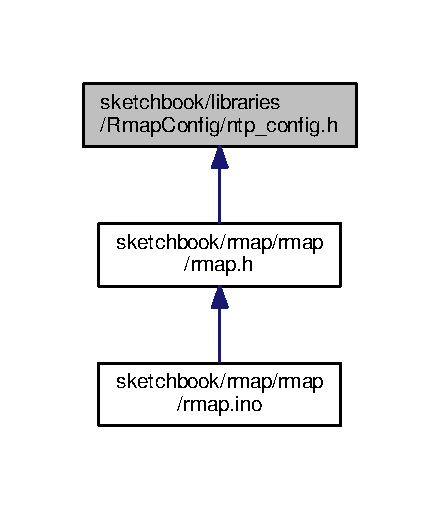
\includegraphics[width=211pt]{ntp__config_8h__dep__incl}
\end{center}
\end{figure}
\subsection*{Macros}
\begin{DoxyCompactItemize}
\item 
\mbox{\Hypertarget{ntp__config_8h_a54153a6aa87c606f585ab167661b1be2}\label{ntp__config_8h_a54153a6aa87c606f585ab167661b1be2}} 
\#define \hyperlink{ntp__config_8h_a54153a6aa87c606f585ab167661b1be2}{N\+T\+P\+\_\+\+S\+E\+R\+V\+E\+R\+\_\+\+L\+E\+N\+G\+TH}~(30)
\begin{DoxyCompactList}\small\item\em Length in bytes for ntp server data buffer. \end{DoxyCompactList}\item 
\mbox{\Hypertarget{ntp__config_8h_ac2609c1adfd1a279c59fed52b5827fd3}\label{ntp__config_8h_ac2609c1adfd1a279c59fed52b5827fd3}} 
\#define \hyperlink{ntp__config_8h_ac2609c1adfd1a279c59fed52b5827fd3}{N\+T\+P\+\_\+\+D\+E\+F\+A\+U\+L\+T\+\_\+\+S\+E\+R\+V\+ER}~(\char`\"{}pool.\+ntp.\+org\char`\"{})
\begin{DoxyCompactList}\small\item\em Default N\+TP server. \end{DoxyCompactList}\end{DoxyCompactItemize}

\hypertarget{sdcard__config_8h}{}\section{sketchbook/libraries/\+Rmap\+Config/sdcard\+\_\+config.h File Reference}
\label{sdcard__config_8h}\index{sketchbook/libraries/\+Rmap\+Config/sdcard\+\_\+config.\+h@{sketchbook/libraries/\+Rmap\+Config/sdcard\+\_\+config.\+h}}
This graph shows which files directly or indirectly include this file\+:\nopagebreak
\begin{figure}[H]
\begin{center}
\leavevmode
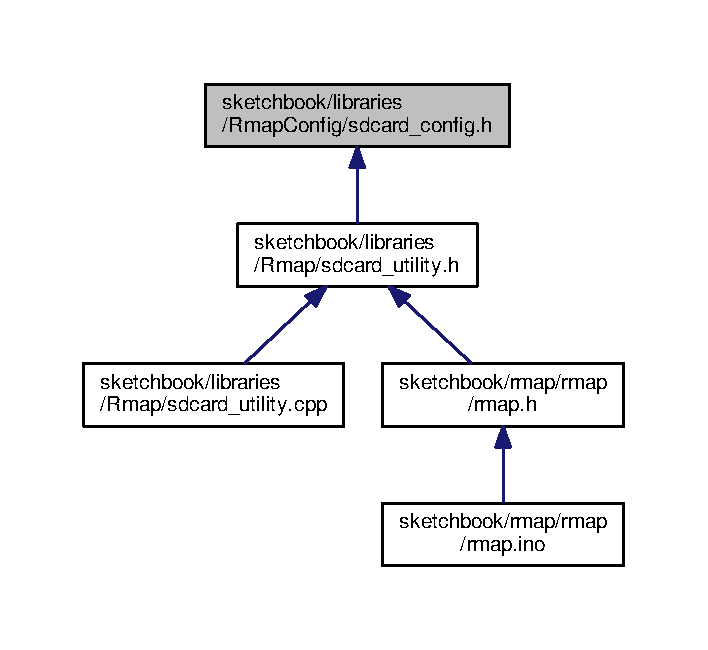
\includegraphics[width=226pt]{sdcard__config_8h__dep__incl}
\end{center}
\end{figure}
\subsection*{Macros}
\begin{DoxyCompactItemize}
\item 
\mbox{\Hypertarget{sdcard__config_8h_ab804055532120d07f54be6620c2f04b5}\label{sdcard__config_8h_ab804055532120d07f54be6620c2f04b5}} 
\#define \hyperlink{sdcard__config_8h_ab804055532120d07f54be6620c2f04b5}{S\+D\+C\+A\+R\+D\+\_\+\+F\+I\+L\+E\+S\+\_\+\+N\+A\+M\+E\+\_\+\+M\+A\+X\+\_\+\+L\+E\+N\+G\+TH}~(20)
\begin{DoxyCompactList}\small\item\em Length in bytes for sdcard file name data buffer. \end{DoxyCompactList}\end{DoxyCompactItemize}

\hypertarget{sensors__config_8h}{}\section{sketchbook/libraries/\+Rmap\+Config/sensors\+\_\+config.h File Reference}
\label{sensors__config_8h}\index{sketchbook/libraries/\+Rmap\+Config/sensors\+\_\+config.\+h@{sketchbook/libraries/\+Rmap\+Config/sensors\+\_\+config.\+h}}
This graph shows which files directly or indirectly include this file\+:\nopagebreak
\begin{figure}[H]
\begin{center}
\leavevmode
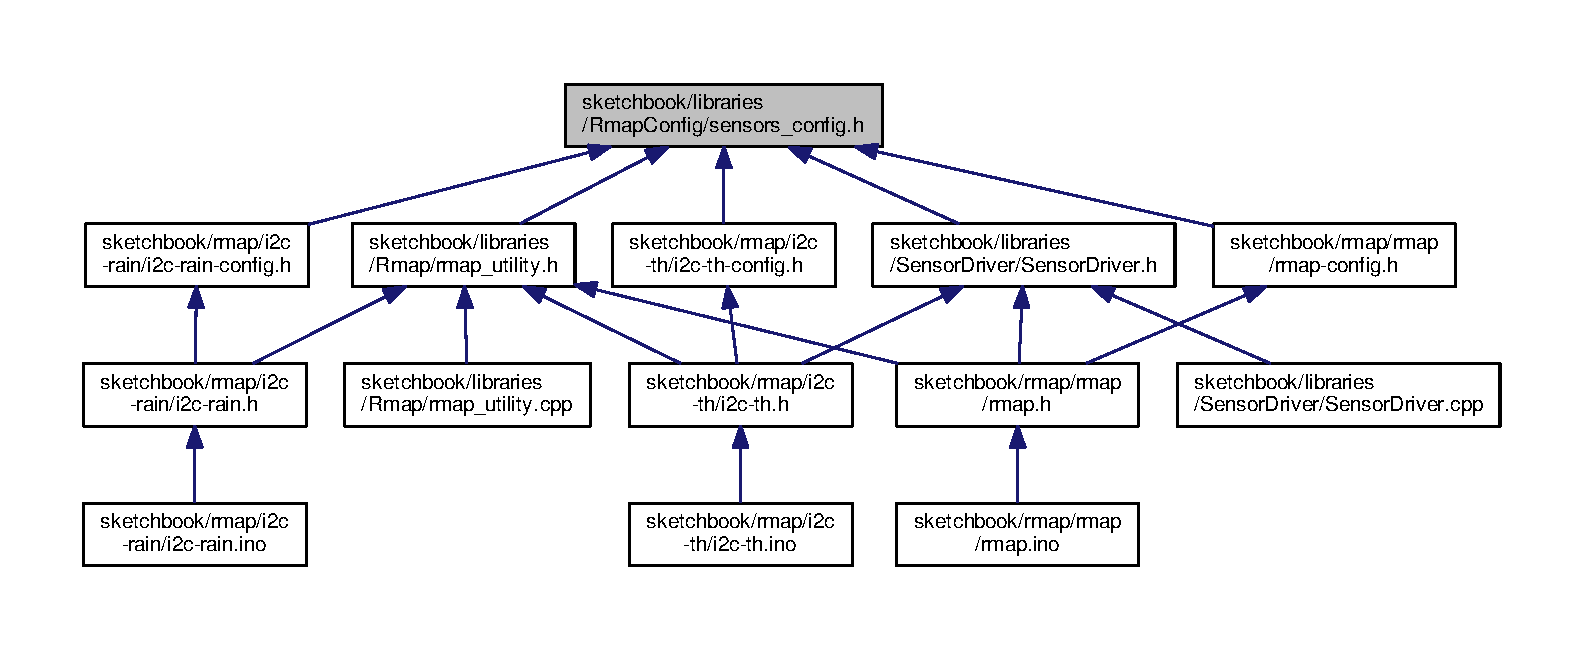
\includegraphics[width=350pt]{sensors__config_8h__dep__incl}
\end{center}
\end{figure}
\subsection*{Macros}
\begin{DoxyCompactItemize}
\item 
\mbox{\Hypertarget{sensors__config_8h_a4f1ecf636dc6d92f75c943c325346bf0}\label{sensors__config_8h_a4f1ecf636dc6d92f75c943c325346bf0}} 
\#define \hyperlink{sensors__config_8h_a4f1ecf636dc6d92f75c943c325346bf0}{U\+S\+E\+\_\+\+J\+S\+ON}~(true)
\begin{DoxyCompactList}\small\item\em Enable if you want use json library for json response (get\+Json function in \hyperlink{classSensorDriver}{Sensor\+Driver}). \end{DoxyCompactList}\item 
\mbox{\Hypertarget{sensors__config_8h_a34acfad25488d28951ff729ebda66311}\label{sensors__config_8h_a34acfad25488d28951ff729ebda66311}} 
\#define \hyperlink{sensors__config_8h_a34acfad25488d28951ff729ebda66311}{U\+S\+E\+\_\+\+S\+E\+N\+S\+O\+R\+\_\+\+A\+DT}~(false)
\begin{DoxyCompactList}\small\item\em Enable if you want use A\+D\+T7420 sensor. \end{DoxyCompactList}\item 
\mbox{\Hypertarget{sensors__config_8h_aa1d83db2373ab5e74ed832abf1b7f0ed}\label{sensors__config_8h_aa1d83db2373ab5e74ed832abf1b7f0ed}} 
\#define \hyperlink{sensors__config_8h_aa1d83db2373ab5e74ed832abf1b7f0ed}{U\+S\+E\+\_\+\+S\+E\+N\+S\+O\+R\+\_\+\+H\+IH}~(false)
\begin{DoxyCompactList}\small\item\em Enable if you want use H\+I\+H6100 sensor. \end{DoxyCompactList}\item 
\mbox{\Hypertarget{sensors__config_8h_a85f2976107ff26789b268febf87a392a}\label{sensors__config_8h_a85f2976107ff26789b268febf87a392a}} 
\#define \hyperlink{sensors__config_8h_a85f2976107ff26789b268febf87a392a}{U\+S\+E\+\_\+\+S\+E\+N\+S\+O\+R\+\_\+\+H\+YT}~(false)
\begin{DoxyCompactList}\small\item\em Enable if you want use H\+Y\+T271 or H\+Y\+T221 sensor. \end{DoxyCompactList}\item 
\mbox{\Hypertarget{sensors__config_8h_a41a207ce017a43c492f8d2a0bf11a598}\label{sensors__config_8h_a41a207ce017a43c492f8d2a0bf11a598}} 
\#define \hyperlink{sensors__config_8h_a41a207ce017a43c492f8d2a0bf11a598}{U\+S\+E\+\_\+\+S\+E\+N\+S\+O\+R\+\_\+\+D\+EP}~(true)
\begin{DoxyCompactList}\small\item\em Enable if you want use Digit\+Eco Power sensor. \end{DoxyCompactList}\item 
\mbox{\Hypertarget{sensors__config_8h_a96ef78fdc773cf6bd675ea2b997e7bc8}\label{sensors__config_8h_a96ef78fdc773cf6bd675ea2b997e7bc8}} 
\#define \hyperlink{sensors__config_8h_a96ef78fdc773cf6bd675ea2b997e7bc8}{U\+S\+E\+\_\+\+S\+E\+N\+S\+O\+R\+\_\+\+H\+I7}~(false)
\begin{DoxyCompactList}\small\item\em Enable if you want use S\+I7021 sensor. \end{DoxyCompactList}\item 
\mbox{\Hypertarget{sensors__config_8h_aee913ac1d68a27f752c81be85b0fc922}\label{sensors__config_8h_aee913ac1d68a27f752c81be85b0fc922}} 
\#define \hyperlink{sensors__config_8h_aee913ac1d68a27f752c81be85b0fc922}{U\+S\+E\+\_\+\+S\+E\+N\+S\+O\+R\+\_\+\+B\+MP}~(false)
\begin{DoxyCompactList}\small\item\em Enable if you want use Bmp085 sensor. \end{DoxyCompactList}\item 
\mbox{\Hypertarget{sensors__config_8h_af719cba7600d5cfeca9911fa9ac23c2d}\label{sensors__config_8h_af719cba7600d5cfeca9911fa9ac23c2d}} 
\#define \hyperlink{sensors__config_8h_af719cba7600d5cfeca9911fa9ac23c2d}{U\+S\+E\+\_\+\+S\+E\+N\+S\+O\+R\+\_\+\+D\+W1}~(false)
\begin{DoxyCompactList}\small\item\em Enable if you want use D\+W1 sensor. \end{DoxyCompactList}\item 
\mbox{\Hypertarget{sensors__config_8h_a7d0abdd8465288cd55c86d95ad466cc7}\label{sensors__config_8h_a7d0abdd8465288cd55c86d95ad466cc7}} 
\#define \hyperlink{sensors__config_8h_a7d0abdd8465288cd55c86d95ad466cc7}{U\+S\+E\+\_\+\+S\+E\+N\+S\+O\+R\+\_\+\+T\+BS}~(false)
\begin{DoxyCompactList}\small\item\em Enable if you want use Tipping bucket rain gauge sensor. \end{DoxyCompactList}\item 
\mbox{\Hypertarget{sensors__config_8h_aba1fe603fab2f047ac3913e33b6f8cce}\label{sensors__config_8h_aba1fe603fab2f047ac3913e33b6f8cce}} 
\#define \hyperlink{sensors__config_8h_aba1fe603fab2f047ac3913e33b6f8cce}{U\+S\+E\+\_\+\+S\+E\+N\+S\+O\+R\+\_\+\+T\+BR}~(true)
\begin{DoxyCompactList}\small\item\em Enable if you want use Tipping bucket rain gauge sensor. \end{DoxyCompactList}\item 
\mbox{\Hypertarget{sensors__config_8h_ace8347c09c95d3fddbaee10e0f2fcb55}\label{sensors__config_8h_ace8347c09c95d3fddbaee10e0f2fcb55}} 
\#define \hyperlink{sensors__config_8h_ace8347c09c95d3fddbaee10e0f2fcb55}{U\+S\+E\+\_\+\+S\+E\+N\+S\+O\+R\+\_\+\+S\+TH}~(false)
\begin{DoxyCompactList}\small\item\em Enable if you want use Temperature and humidity oneshot sensor. \end{DoxyCompactList}\item 
\mbox{\Hypertarget{sensors__config_8h_a22d6a7857098158d20b37de9080accb5}\label{sensors__config_8h_a22d6a7857098158d20b37de9080accb5}} 
\#define \hyperlink{sensors__config_8h_a22d6a7857098158d20b37de9080accb5}{U\+S\+E\+\_\+\+S\+E\+N\+S\+O\+R\+\_\+\+I\+TH}~(true)
\begin{DoxyCompactList}\small\item\em Enable if you want use Temperature and humidity continuous istantaneous sensor. \end{DoxyCompactList}\item 
\mbox{\Hypertarget{sensors__config_8h_a10ed05c0989cac98ec0dcccafe5eab2d}\label{sensors__config_8h_a10ed05c0989cac98ec0dcccafe5eab2d}} 
\#define \hyperlink{sensors__config_8h_a10ed05c0989cac98ec0dcccafe5eab2d}{U\+S\+E\+\_\+\+S\+E\+N\+S\+O\+R\+\_\+\+N\+TH}~(true)
\begin{DoxyCompactList}\small\item\em Enable if you want use Temperature and humidity continuous minium sensor. \end{DoxyCompactList}\item 
\mbox{\Hypertarget{sensors__config_8h_a716f318739d3cc63bbe11a711152a93f}\label{sensors__config_8h_a716f318739d3cc63bbe11a711152a93f}} 
\#define \hyperlink{sensors__config_8h_a716f318739d3cc63bbe11a711152a93f}{U\+S\+E\+\_\+\+S\+E\+N\+S\+O\+R\+\_\+\+M\+TH}~(true)
\begin{DoxyCompactList}\small\item\em Enable if you want use Temperature and humidity continuous average sensor. \end{DoxyCompactList}\item 
\mbox{\Hypertarget{sensors__config_8h_a31485d4f9fa38af9114e6bd1455e989c}\label{sensors__config_8h_a31485d4f9fa38af9114e6bd1455e989c}} 
\#define \hyperlink{sensors__config_8h_a31485d4f9fa38af9114e6bd1455e989c}{U\+S\+E\+\_\+\+S\+E\+N\+S\+O\+R\+\_\+\+X\+TH}~(true)
\begin{DoxyCompactList}\small\item\em Enable if you want use Temperature and humidity continuous maximum sensor. \end{DoxyCompactList}\item 
\mbox{\Hypertarget{sensors__config_8h_a095a19c70916bf36a45398d52b3e294e}\label{sensors__config_8h_a095a19c70916bf36a45398d52b3e294e}} 
\#define \hyperlink{sensors__config_8h_a095a19c70916bf36a45398d52b3e294e}{U\+S\+E\+\_\+\+S\+E\+N\+S\+O\+R\+\_\+\+S\+SD}~(false)
\begin{DoxyCompactList}\small\item\em Enable if you want use S\+S\+D011 oneshot sensor. \end{DoxyCompactList}\item 
\mbox{\Hypertarget{sensors__config_8h_ace417a5dfc761d0765409b5d9fb40c5e}\label{sensors__config_8h_ace417a5dfc761d0765409b5d9fb40c5e}} 
\#define \hyperlink{sensors__config_8h_ace417a5dfc761d0765409b5d9fb40c5e}{U\+S\+E\+\_\+\+S\+E\+N\+S\+O\+R\+\_\+\+I\+SD}~(false)
\begin{DoxyCompactList}\small\item\em Enable if you want use S\+S\+D011 report istantaneous sensor. \end{DoxyCompactList}\item 
\mbox{\Hypertarget{sensors__config_8h_a067b2396a85b7932fcf73b6b9c80408c}\label{sensors__config_8h_a067b2396a85b7932fcf73b6b9c80408c}} 
\#define \hyperlink{sensors__config_8h_a067b2396a85b7932fcf73b6b9c80408c}{U\+S\+E\+\_\+\+S\+E\+N\+S\+O\+R\+\_\+\+N\+SD}~(false)
\begin{DoxyCompactList}\small\item\em Enable if you want use S\+S\+D011 report minium sensor. \end{DoxyCompactList}\item 
\mbox{\Hypertarget{sensors__config_8h_a80e1f8a3db337f39a4ec046e88455692}\label{sensors__config_8h_a80e1f8a3db337f39a4ec046e88455692}} 
\#define \hyperlink{sensors__config_8h_a80e1f8a3db337f39a4ec046e88455692}{U\+S\+E\+\_\+\+S\+E\+N\+S\+O\+R\+\_\+\+M\+SD}~(false)
\begin{DoxyCompactList}\small\item\em Enable if you want use S\+S\+D011 report average sensor. \end{DoxyCompactList}\item 
\mbox{\Hypertarget{sensors__config_8h_aee2170fca2d187e633b8ad17b0f86d8f}\label{sensors__config_8h_aee2170fca2d187e633b8ad17b0f86d8f}} 
\#define \hyperlink{sensors__config_8h_aee2170fca2d187e633b8ad17b0f86d8f}{U\+S\+E\+\_\+\+S\+E\+N\+S\+O\+R\+\_\+\+X\+SD}~(false)
\begin{DoxyCompactList}\small\item\em Enable if you want use S\+S\+D011 report maximum sensor. \end{DoxyCompactList}\item 
\mbox{\Hypertarget{sensors__config_8h_a4a69ad5f9e0cd1e81808b7a9bf8922a7}\label{sensors__config_8h_a4a69ad5f9e0cd1e81808b7a9bf8922a7}} 
\#define \hyperlink{sensors__config_8h_a4a69ad5f9e0cd1e81808b7a9bf8922a7}{U\+S\+E\+\_\+\+S\+E\+N\+S\+O\+R\+\_\+\+S\+MI}~(false)
\begin{DoxyCompactList}\small\item\em Enable if you want use M\+I\+C\+S4514 oneshot sensor. \end{DoxyCompactList}\item 
\mbox{\Hypertarget{sensors__config_8h_a5d18292e50afd3fb2189c68831acada4}\label{sensors__config_8h_a5d18292e50afd3fb2189c68831acada4}} 
\#define \hyperlink{sensors__config_8h_a5d18292e50afd3fb2189c68831acada4}{U\+S\+E\+\_\+\+S\+E\+N\+S\+O\+R\+\_\+\+I\+MI}~(false)
\begin{DoxyCompactList}\small\item\em Enable if you want use M\+I\+C\+S4514 report istantaneous sensor. \end{DoxyCompactList}\item 
\mbox{\Hypertarget{sensors__config_8h_ab8f8d09065d18c9a172348237b9c28e1}\label{sensors__config_8h_ab8f8d09065d18c9a172348237b9c28e1}} 
\#define \hyperlink{sensors__config_8h_ab8f8d09065d18c9a172348237b9c28e1}{U\+S\+E\+\_\+\+S\+E\+N\+S\+O\+R\+\_\+\+N\+MI}~(false)
\begin{DoxyCompactList}\small\item\em Enable if you want use M\+I\+C\+S4514 report minium sensor. \end{DoxyCompactList}\item 
\mbox{\Hypertarget{sensors__config_8h_a0115de59ffaf7ea7841a413f3e59b54a}\label{sensors__config_8h_a0115de59ffaf7ea7841a413f3e59b54a}} 
\#define \hyperlink{sensors__config_8h_a0115de59ffaf7ea7841a413f3e59b54a}{U\+S\+E\+\_\+\+S\+E\+N\+S\+O\+R\+\_\+\+M\+MI}~(false)
\begin{DoxyCompactList}\small\item\em Enable if you want use M\+I\+C\+S4514 report average sensor. \end{DoxyCompactList}\item 
\mbox{\Hypertarget{sensors__config_8h_ae329aa524de76428bcaa097eb798ed3b}\label{sensors__config_8h_ae329aa524de76428bcaa097eb798ed3b}} 
\#define \hyperlink{sensors__config_8h_ae329aa524de76428bcaa097eb798ed3b}{U\+S\+E\+\_\+\+S\+E\+N\+S\+O\+R\+\_\+\+X\+MI}~(false)
\begin{DoxyCompactList}\small\item\em Enable if you want use M\+I\+C\+S4514 report maximum sensor. \end{DoxyCompactList}\item 
\mbox{\Hypertarget{sensors__config_8h_ae53e68cc3e340f3c2a6930a78ca09c7c}\label{sensors__config_8h_ae53e68cc3e340f3c2a6930a78ca09c7c}} 
\#define \hyperlink{sensors__config_8h_ae53e68cc3e340f3c2a6930a78ca09c7c}{U\+S\+E\+\_\+\+S\+E\+N\+S\+O\+R\+\_\+\+R\+F24}~(false)
\begin{DoxyCompactList}\small\item\em Enable if you want use Radio R\+F24 sensor. \end{DoxyCompactList}\item 
\mbox{\Hypertarget{sensors__config_8h_a6296edf2c03225032bf69757340ed387}\label{sensors__config_8h_a6296edf2c03225032bf69757340ed387}} 
\#define \hyperlink{sensors__config_8h_a6296edf2c03225032bf69757340ed387}{R\+A\+I\+N\+\_\+\+F\+O\+R\+\_\+\+T\+IP}~(1)
\begin{DoxyCompactList}\small\item\em How much mm of rain for one tip of tipping bucket rain gauge. \end{DoxyCompactList}\item 
\#define \hyperlink{sensors__config_8h_a84d7e30b4b359d20293dc9db0b338a5c}{V\+A\+L\+U\+E\+S\+\_\+\+T\+O\+\_\+\+R\+E\+A\+D\+\_\+\+F\+R\+O\+M\+\_\+\+S\+E\+N\+S\+O\+R\+\_\+\+C\+O\+U\+NT}~(3)
\item 
\mbox{\Hypertarget{sensors__config_8h_acd6a77ef70e6cd768267a4e3d79cf981}\label{sensors__config_8h_acd6a77ef70e6cd768267a4e3d79cf981}} 
\#define \hyperlink{sensors__config_8h_acd6a77ef70e6cd768267a4e3d79cf981}{O\+B\+S\+E\+R\+V\+A\+T\+I\+O\+N\+S\+\_\+\+M\+I\+N\+U\+T\+ES}~(1)
\begin{DoxyCompactList}\small\item\em How much minutes for calculate an observations by processing sampling. Tipically 1-\/10 minutes. \end{DoxyCompactList}\item 
\mbox{\Hypertarget{sensors__config_8h_a8c9d131a88fa3910b344007003f0f417}\label{sensors__config_8h_a8c9d131a88fa3910b344007003f0f417}} 
\#define \hyperlink{sensors__config_8h_a8c9d131a88fa3910b344007003f0f417}{S\+T\+A\+T\+I\+S\+T\+I\+C\+A\+L\+\_\+\+D\+A\+T\+A\+\_\+\+C\+O\+U\+NT}~(15)
\begin{DoxyCompactList}\small\item\em How much observations are needed for generating a report. \end{DoxyCompactList}\item 
\mbox{\Hypertarget{sensors__config_8h_a59ca9f7c75d5ef71f2292b4f8e136159}\label{sensors__config_8h_a59ca9f7c75d5ef71f2292b4f8e136159}} 
\#define \hyperlink{sensors__config_8h_a59ca9f7c75d5ef71f2292b4f8e136159}{O\+B\+S\+E\+R\+V\+A\+T\+I\+O\+N\+\_\+\+C\+O\+U\+NT}~(60)
\begin{DoxyCompactList}\small\item\em How much observations were stored in ram. \end{DoxyCompactList}\item 
\mbox{\Hypertarget{sensors__config_8h_a335ea2e7e5bc1aeec20ac2433232aaf3}\label{sensors__config_8h_a335ea2e7e5bc1aeec20ac2433232aaf3}} 
\#define \hyperlink{sensors__config_8h_a335ea2e7e5bc1aeec20ac2433232aaf3}{O\+B\+S\+E\+R\+V\+A\+T\+I\+O\+N\+\_\+\+C\+O\+U\+N\+T\+\_\+\+T\+O\+L\+L\+E\+R\+A\+N\+CE}~(2)
\begin{DoxyCompactList}\small\item\em Tolerance of observations for generating a valid report. \end{DoxyCompactList}\end{DoxyCompactItemize}


\subsection{Macro Definition Documentation}
\mbox{\Hypertarget{sensors__config_8h_a84d7e30b4b359d20293dc9db0b338a5c}\label{sensors__config_8h_a84d7e30b4b359d20293dc9db0b338a5c}} 
\index{sensors\+\_\+config.\+h@{sensors\+\_\+config.\+h}!V\+A\+L\+U\+E\+S\+\_\+\+T\+O\+\_\+\+R\+E\+A\+D\+\_\+\+F\+R\+O\+M\+\_\+\+S\+E\+N\+S\+O\+R\+\_\+\+C\+O\+U\+NT@{V\+A\+L\+U\+E\+S\+\_\+\+T\+O\+\_\+\+R\+E\+A\+D\+\_\+\+F\+R\+O\+M\+\_\+\+S\+E\+N\+S\+O\+R\+\_\+\+C\+O\+U\+NT}}
\index{V\+A\+L\+U\+E\+S\+\_\+\+T\+O\+\_\+\+R\+E\+A\+D\+\_\+\+F\+R\+O\+M\+\_\+\+S\+E\+N\+S\+O\+R\+\_\+\+C\+O\+U\+NT@{V\+A\+L\+U\+E\+S\+\_\+\+T\+O\+\_\+\+R\+E\+A\+D\+\_\+\+F\+R\+O\+M\+\_\+\+S\+E\+N\+S\+O\+R\+\_\+\+C\+O\+U\+NT}!sensors\+\_\+config.\+h@{sensors\+\_\+config.\+h}}
\subsubsection{\texorpdfstring{V\+A\+L\+U\+E\+S\+\_\+\+T\+O\+\_\+\+R\+E\+A\+D\+\_\+\+F\+R\+O\+M\+\_\+\+S\+E\+N\+S\+O\+R\+\_\+\+C\+O\+U\+NT}{VALUES\_TO\_READ\_FROM\_SENSOR\_COUNT}}
{\footnotesize\ttfamily \#define V\+A\+L\+U\+E\+S\+\_\+\+T\+O\+\_\+\+R\+E\+A\+D\+\_\+\+F\+R\+O\+M\+\_\+\+S\+E\+N\+S\+O\+R\+\_\+\+C\+O\+U\+NT~(3)}

Maximum number of values to be read by the sensors. 
\hypertarget{SensorDriver_8cpp}{}\section{sketchbook/libraries/\+Sensor\+Driver/\+Sensor\+Driver.cpp File Reference}
\label{SensorDriver_8cpp}\index{sketchbook/libraries/\+Sensor\+Driver/\+Sensor\+Driver.\+cpp@{sketchbook/libraries/\+Sensor\+Driver/\+Sensor\+Driver.\+cpp}}
{\ttfamily \#include $<$debug\+\_\+config.\+h$>$}\newline
{\ttfamily \#include \char`\"{}Sensor\+Driver.\+h\char`\"{}}\newline
Include dependency graph for Sensor\+Driver.\+cpp\+:\nopagebreak
\begin{figure}[H]
\begin{center}
\leavevmode
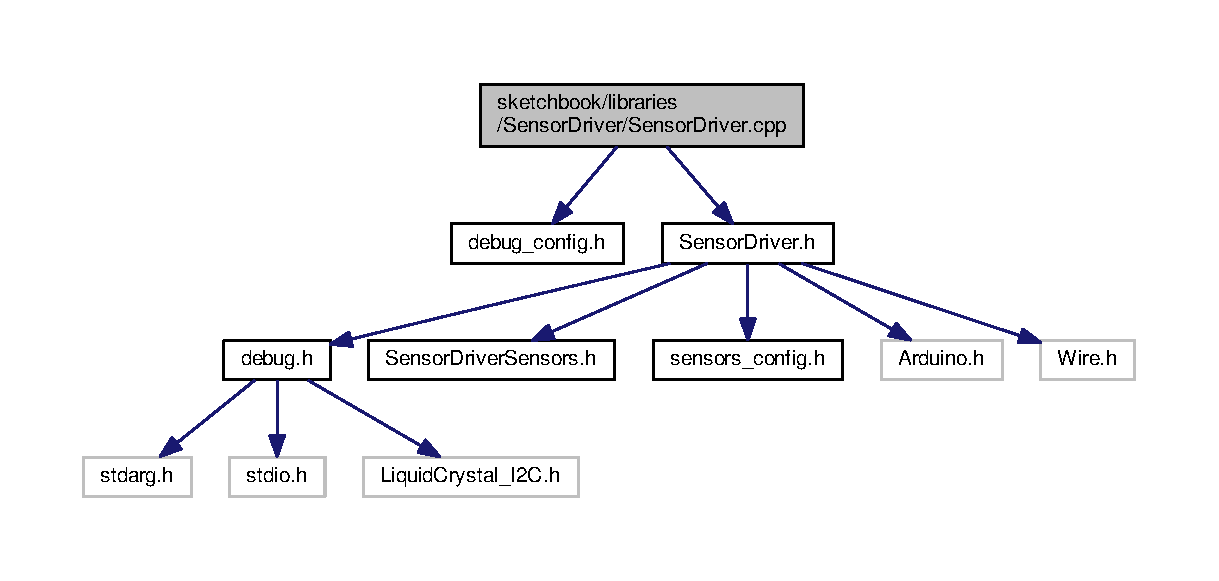
\includegraphics[width=350pt]{SensorDriver_8cpp__incl}
\end{center}
\end{figure}
\subsection*{Macros}
\begin{DoxyCompactItemize}
\item 
\mbox{\Hypertarget{SensorDriver_8cpp_a31fa5c36fa17c66feec7a67b76c3e786}\label{SensorDriver_8cpp_a31fa5c36fa17c66feec7a67b76c3e786}} 
\#define \hyperlink{SensorDriver_8cpp_a31fa5c36fa17c66feec7a67b76c3e786}{S\+E\+R\+I\+A\+L\+\_\+\+T\+R\+A\+C\+E\+\_\+\+L\+E\+V\+EL}~\hyperlink{debug__config_8h_a94cfa13ad63cfb5a454d6ca5f2394efd}{S\+E\+N\+S\+O\+R\+\_\+\+D\+R\+I\+V\+E\+R\+\_\+\+S\+E\+R\+I\+A\+L\+\_\+\+T\+R\+A\+C\+E\+\_\+\+L\+E\+V\+EL}
\begin{DoxyCompactList}\small\item\em Serial debug level for this library. \end{DoxyCompactList}\end{DoxyCompactItemize}

\hypertarget{SensorDriver_8h}{}\section{sketchbook/libraries/\+Sensor\+Driver/\+Sensor\+Driver.h File Reference}
\label{SensorDriver_8h}\index{sketchbook/libraries/\+Sensor\+Driver/\+Sensor\+Driver.\+h@{sketchbook/libraries/\+Sensor\+Driver/\+Sensor\+Driver.\+h}}
{\ttfamily \#include $<$debug.\+h$>$}\newline
{\ttfamily \#include \char`\"{}Sensor\+Driver\+Sensors.\+h\char`\"{}}\newline
{\ttfamily \#include $<$sensors\+\_\+config.\+h$>$}\newline
{\ttfamily \#include $<$Arduino.\+h$>$}\newline
{\ttfamily \#include $<$Wire.\+h$>$}\newline
Include dependency graph for Sensor\+Driver.\+h\+:\nopagebreak
\begin{figure}[H]
\begin{center}
\leavevmode
\includegraphics[width=350pt]{SensorDriver_8h__incl}
\end{center}
\end{figure}
This graph shows which files directly or indirectly include this file\+:\nopagebreak
\begin{figure}[H]
\begin{center}
\leavevmode
\includegraphics[width=350pt]{SensorDriver_8h__dep__incl}
\end{center}
\end{figure}
\subsection*{Classes}
\begin{DoxyCompactItemize}
\item 
class \hyperlink{classSensorDriver}{Sensor\+Driver}
\begin{DoxyCompactList}\small\item\em \hyperlink{classSensorDriver}{Sensor\+Driver} class. \end{DoxyCompactList}\end{DoxyCompactItemize}
\subsection*{Macros}
\begin{DoxyCompactItemize}
\item 
\mbox{\Hypertarget{SensorDriver_8h_a07fe35e3dc528b2f925554c55cd24664}\label{SensorDriver_8h_a07fe35e3dc528b2f925554c55cd24664}} 
\#define \hyperlink{SensorDriver_8h_a07fe35e3dc528b2f925554c55cd24664}{S\+E\+N\+S\+O\+R\+\_\+\+D\+R\+I\+V\+E\+R\+\_\+\+E\+R\+R\+OR}~(1)
\begin{DoxyCompactList}\small\item\em Sensor driver\textquotesingle{}s error state. \end{DoxyCompactList}\item 
\mbox{\Hypertarget{SensorDriver_8h_a74298d24491e2bbf82daec9d66010dab}\label{SensorDriver_8h_a74298d24491e2bbf82daec9d66010dab}} 
\#define \hyperlink{SensorDriver_8h_a74298d24491e2bbf82daec9d66010dab}{S\+E\+N\+S\+O\+R\+\_\+\+D\+R\+I\+V\+E\+R\+\_\+\+S\+U\+C\+C\+E\+SS}~(0)
\begin{DoxyCompactList}\small\item\em Sensor driver\textquotesingle{}s success state. \end{DoxyCompactList}\item 
\mbox{\Hypertarget{SensorDriver_8h_ab4d5100af791824917d23d864af93435}\label{SensorDriver_8h_ab4d5100af791824917d23d864af93435}} 
\#define \hyperlink{SensorDriver_8h_ab4d5100af791824917d23d864af93435}{S\+E\+N\+S\+O\+R\+\_\+\+D\+R\+I\+V\+E\+R\+\_\+\+C\+\_\+\+T\+O\+\_\+K}~(27315l)
\begin{DoxyCompactList}\small\item\em Kelvin to Celsius constant conversion. \end{DoxyCompactList}\end{DoxyCompactItemize}

\hypertarget{SensorDriverSensors_8h}{}\section{sketchbook/libraries/\+Sensor\+Driver/\+Sensor\+Driver\+Sensors.h File Reference}
\label{SensorDriverSensors_8h}\index{sketchbook/libraries/\+Sensor\+Driver/\+Sensor\+Driver\+Sensors.\+h@{sketchbook/libraries/\+Sensor\+Driver/\+Sensor\+Driver\+Sensors.\+h}}
This graph shows which files directly or indirectly include this file\+:\nopagebreak
\begin{figure}[H]
\begin{center}
\leavevmode
\includegraphics[width=350pt]{SensorDriverSensors_8h__dep__incl}
\end{center}
\end{figure}
\subsection*{Macros}
\begin{DoxyCompactItemize}
\item 
\mbox{\Hypertarget{SensorDriverSensors_8h_a8eed23ad13ab23b0f3cc67af6cfc7af0}\label{SensorDriverSensors_8h_a8eed23ad13ab23b0f3cc67af6cfc7af0}} 
\#define \hyperlink{SensorDriverSensors_8h_a8eed23ad13ab23b0f3cc67af6cfc7af0}{S\+E\+N\+S\+O\+R\+\_\+\+D\+R\+I\+V\+E\+R\+\_\+\+I2C}~(\char`\"{}I2C\char`\"{})
\begin{DoxyCompactList}\small\item\em Sensor driver\textquotesingle{}s I2C driver. \end{DoxyCompactList}\item 
\mbox{\Hypertarget{SensorDriverSensors_8h_ab2e97f514918a0ed5d100d8fd57e8062}\label{SensorDriverSensors_8h_ab2e97f514918a0ed5d100d8fd57e8062}} 
\#define \hyperlink{SensorDriverSensors_8h_ab2e97f514918a0ed5d100d8fd57e8062}{S\+E\+N\+S\+O\+R\+\_\+\+T\+Y\+P\+E\+\_\+\+A\+DT}~(\char`\"{}A\+DT\char`\"{})
\begin{DoxyCompactList}\small\item\em Sensor driver\textquotesingle{}s A\+DT sensor type for A\+D\+T7420. \end{DoxyCompactList}\item 
\mbox{\Hypertarget{SensorDriverSensors_8h_abafb7060a78a2d0a44303ba9b89d467c}\label{SensorDriverSensors_8h_abafb7060a78a2d0a44303ba9b89d467c}} 
\#define \hyperlink{SensorDriverSensors_8h_abafb7060a78a2d0a44303ba9b89d467c}{S\+E\+N\+S\+O\+R\+\_\+\+T\+Y\+P\+E\+\_\+\+H\+IH}~(\char`\"{}H\+IH\char`\"{})
\begin{DoxyCompactList}\small\item\em Sensor driver\textquotesingle{}s H\+IH sensor type for H\+I\+H6100. \end{DoxyCompactList}\item 
\mbox{\Hypertarget{SensorDriverSensors_8h_a7b688581b89ed23ae7a51b90397cb995}\label{SensorDriverSensors_8h_a7b688581b89ed23ae7a51b90397cb995}} 
\#define \hyperlink{SensorDriverSensors_8h_a7b688581b89ed23ae7a51b90397cb995}{S\+E\+N\+S\+O\+R\+\_\+\+T\+Y\+P\+E\+\_\+\+H\+YT}~(\char`\"{}H\+YT\char`\"{})
\begin{DoxyCompactList}\small\item\em Sensor driver\textquotesingle{}s H\+YT sensor type for H\+Y\+T271 and H\+Y\+T221. \end{DoxyCompactList}\item 
\mbox{\Hypertarget{SensorDriverSensors_8h_a62effb2a961f745204a3d51f5126033b}\label{SensorDriverSensors_8h_a62effb2a961f745204a3d51f5126033b}} 
\#define \hyperlink{SensorDriverSensors_8h_a62effb2a961f745204a3d51f5126033b}{S\+E\+N\+S\+O\+R\+\_\+\+T\+Y\+P\+E\+\_\+\+D\+EP}~(\char`\"{}D\+EP\char`\"{})
\begin{DoxyCompactList}\small\item\em Sensor driver\textquotesingle{}s D\+EP sensor type for Digit\+Eco Power. \end{DoxyCompactList}\item 
\mbox{\Hypertarget{SensorDriverSensors_8h_a75c6c036f460bc19771264ceda04a8fa}\label{SensorDriverSensors_8h_a75c6c036f460bc19771264ceda04a8fa}} 
\#define \hyperlink{SensorDriverSensors_8h_a75c6c036f460bc19771264ceda04a8fa}{S\+E\+N\+S\+O\+R\+\_\+\+T\+Y\+P\+E\+\_\+\+H\+I7}~(\char`\"{}H\+I7\char`\"{})
\begin{DoxyCompactList}\small\item\em Sensor driver\textquotesingle{}s H\+I7 sensor type for S\+I7021. \end{DoxyCompactList}\item 
\mbox{\Hypertarget{SensorDriverSensors_8h_a6dd28050066d5576c375fe620be470dd}\label{SensorDriverSensors_8h_a6dd28050066d5576c375fe620be470dd}} 
\#define \hyperlink{SensorDriverSensors_8h_a6dd28050066d5576c375fe620be470dd}{S\+E\+N\+S\+O\+R\+\_\+\+T\+Y\+P\+E\+\_\+\+B\+MP}~(\char`\"{}B\+MP\char`\"{})
\begin{DoxyCompactList}\small\item\em Sensor driver\textquotesingle{}s B\+MP sensor type for Bmp085. \end{DoxyCompactList}\item 
\mbox{\Hypertarget{SensorDriverSensors_8h_a10f115d4f52b061a6c1b71dcb38dfa9f}\label{SensorDriverSensors_8h_a10f115d4f52b061a6c1b71dcb38dfa9f}} 
\#define \hyperlink{SensorDriverSensors_8h_a10f115d4f52b061a6c1b71dcb38dfa9f}{S\+E\+N\+S\+O\+R\+\_\+\+T\+Y\+P\+E\+\_\+\+D\+W1}~(\char`\"{}D\+W1\char`\"{})
\begin{DoxyCompactList}\small\item\em Sensor driver\textquotesingle{}s D\+W1 sensor type for oneshot D\+W1. \end{DoxyCompactList}\item 
\mbox{\Hypertarget{SensorDriverSensors_8h_aff9cfaf44a9e58151321879df14ee029}\label{SensorDriverSensors_8h_aff9cfaf44a9e58151321879df14ee029}} 
\#define \hyperlink{SensorDriverSensors_8h_aff9cfaf44a9e58151321879df14ee029}{S\+E\+N\+S\+O\+R\+\_\+\+T\+Y\+P\+E\+\_\+\+T\+BS}~(\char`\"{}T\+BS\char`\"{})
\begin{DoxyCompactList}\small\item\em Sensor driver\textquotesingle{}s T\+BS sensor type for oneshot tipping bucket rain gauge. \end{DoxyCompactList}\item 
\mbox{\Hypertarget{SensorDriverSensors_8h_ab53c32a82e88feae75991536546256de}\label{SensorDriverSensors_8h_ab53c32a82e88feae75991536546256de}} 
\#define \hyperlink{SensorDriverSensors_8h_ab53c32a82e88feae75991536546256de}{S\+E\+N\+S\+O\+R\+\_\+\+T\+Y\+P\+E\+\_\+\+T\+BR}~(\char`\"{}T\+BR\char`\"{})
\begin{DoxyCompactList}\small\item\em Sensor driver\textquotesingle{}s T\+BR sensor type for oneshot tipping bucket rain gauge. \end{DoxyCompactList}\item 
\mbox{\Hypertarget{SensorDriverSensors_8h_a5802a33d9b9b10d0a1256f5592a41320}\label{SensorDriverSensors_8h_a5802a33d9b9b10d0a1256f5592a41320}} 
\#define \hyperlink{SensorDriverSensors_8h_a5802a33d9b9b10d0a1256f5592a41320}{S\+E\+N\+S\+O\+R\+\_\+\+T\+Y\+P\+E\+\_\+\+S\+TH}~(\char`\"{}S\+TH\char`\"{})
\begin{DoxyCompactList}\small\item\em Sensor driver\textquotesingle{}s S\+TH sensor type for oneshot istantaneous temperature and humidity. \end{DoxyCompactList}\item 
\mbox{\Hypertarget{SensorDriverSensors_8h_af31ca5fe50a1dda29324e2983bdb3a25}\label{SensorDriverSensors_8h_af31ca5fe50a1dda29324e2983bdb3a25}} 
\#define \hyperlink{SensorDriverSensors_8h_af31ca5fe50a1dda29324e2983bdb3a25}{S\+E\+N\+S\+O\+R\+\_\+\+T\+Y\+P\+E\+\_\+\+I\+TH}~(\char`\"{}I\+TH\char`\"{})
\begin{DoxyCompactList}\small\item\em Sensor driver\textquotesingle{}s I\+TH sensor type for continuous istantaneous temperature and humidity. \end{DoxyCompactList}\item 
\mbox{\Hypertarget{SensorDriverSensors_8h_a3660a669e65871b776f6401942b27f2e}\label{SensorDriverSensors_8h_a3660a669e65871b776f6401942b27f2e}} 
\#define \hyperlink{SensorDriverSensors_8h_a3660a669e65871b776f6401942b27f2e}{S\+E\+N\+S\+O\+R\+\_\+\+T\+Y\+P\+E\+\_\+\+M\+TH}~(\char`\"{}M\+TH\char`\"{})
\begin{DoxyCompactList}\small\item\em Sensor driver\textquotesingle{}s M\+TH sensor type for continuous average temperature and humidity. \end{DoxyCompactList}\item 
\mbox{\Hypertarget{SensorDriverSensors_8h_a2b91776cfd66962ee4a5674aaf84091d}\label{SensorDriverSensors_8h_a2b91776cfd66962ee4a5674aaf84091d}} 
\#define \hyperlink{SensorDriverSensors_8h_a2b91776cfd66962ee4a5674aaf84091d}{S\+E\+N\+S\+O\+R\+\_\+\+T\+Y\+P\+E\+\_\+\+N\+TH}~(\char`\"{}N\+TH\char`\"{})
\begin{DoxyCompactList}\small\item\em Sensor driver\textquotesingle{}s N\+TH sensor type for continuous minimum temperature and humidity. \end{DoxyCompactList}\item 
\mbox{\Hypertarget{SensorDriverSensors_8h_a09be1457ad9a46dab2f2323833011814}\label{SensorDriverSensors_8h_a09be1457ad9a46dab2f2323833011814}} 
\#define \hyperlink{SensorDriverSensors_8h_a09be1457ad9a46dab2f2323833011814}{S\+E\+N\+S\+O\+R\+\_\+\+T\+Y\+P\+E\+\_\+\+X\+TH}~(\char`\"{}X\+TH\char`\"{})
\begin{DoxyCompactList}\small\item\em Sensor driver\textquotesingle{}s X\+TH sensor type for continuous maximum temperature and humidity. \end{DoxyCompactList}\item 
\mbox{\Hypertarget{SensorDriverSensors_8h_a3ae3ebf93f91430df24c38b58d538537}\label{SensorDriverSensors_8h_a3ae3ebf93f91430df24c38b58d538537}} 
\#define \hyperlink{SensorDriverSensors_8h_a3ae3ebf93f91430df24c38b58d538537}{S\+E\+N\+S\+O\+R\+\_\+\+T\+Y\+P\+E\+\_\+\+S\+SD}~(\char`\"{}S\+SD\char`\"{})
\begin{DoxyCompactList}\small\item\em Sensor driver\textquotesingle{}s S\+SD sensor type for S\+S\+D011 oneshot. \end{DoxyCompactList}\item 
\mbox{\Hypertarget{SensorDriverSensors_8h_aa231fcf13e123621aabe4188a9ab4692}\label{SensorDriverSensors_8h_aa231fcf13e123621aabe4188a9ab4692}} 
\#define \hyperlink{SensorDriverSensors_8h_aa231fcf13e123621aabe4188a9ab4692}{S\+E\+N\+S\+O\+R\+\_\+\+T\+Y\+P\+E\+\_\+\+I\+SD}~(\char`\"{}I\+SD\char`\"{})
\begin{DoxyCompactList}\small\item\em Sensor driver\textquotesingle{}s I\+SD sensor type for S\+S\+D011 report istantaneous. \end{DoxyCompactList}\item 
\mbox{\Hypertarget{SensorDriverSensors_8h_a7c8698eef2213694e451eddbd547f4f2}\label{SensorDriverSensors_8h_a7c8698eef2213694e451eddbd547f4f2}} 
\#define \hyperlink{SensorDriverSensors_8h_a7c8698eef2213694e451eddbd547f4f2}{S\+E\+N\+S\+O\+R\+\_\+\+T\+Y\+P\+E\+\_\+\+M\+SD}~(\char`\"{}M\+SD\char`\"{})
\begin{DoxyCompactList}\small\item\em Sensor driver\textquotesingle{}s M\+SD sensor type for S\+S\+D011 report average. \end{DoxyCompactList}\item 
\mbox{\Hypertarget{SensorDriverSensors_8h_a79e473204721244fa9e66aafa21425db}\label{SensorDriverSensors_8h_a79e473204721244fa9e66aafa21425db}} 
\#define \hyperlink{SensorDriverSensors_8h_a79e473204721244fa9e66aafa21425db}{S\+E\+N\+S\+O\+R\+\_\+\+T\+Y\+P\+E\+\_\+\+N\+SD}~(\char`\"{}N\+SD\char`\"{})
\begin{DoxyCompactList}\small\item\em Sensor driver\textquotesingle{}s N\+SD sensor type for S\+S\+D011 report minium. \end{DoxyCompactList}\item 
\mbox{\Hypertarget{SensorDriverSensors_8h_a4baeb964adadd3f095ac3d98dccde443}\label{SensorDriverSensors_8h_a4baeb964adadd3f095ac3d98dccde443}} 
\#define \hyperlink{SensorDriverSensors_8h_a4baeb964adadd3f095ac3d98dccde443}{S\+E\+N\+S\+O\+R\+\_\+\+T\+Y\+P\+E\+\_\+\+X\+SD}~(\char`\"{}X\+SD\char`\"{})
\begin{DoxyCompactList}\small\item\em Sensor driver\textquotesingle{}s X\+SD sensor type for S\+S\+D011 report maximum. \end{DoxyCompactList}\item 
\mbox{\Hypertarget{SensorDriverSensors_8h_a91ba1b3be168a1b3263ff5737083a717}\label{SensorDriverSensors_8h_a91ba1b3be168a1b3263ff5737083a717}} 
\#define \hyperlink{SensorDriverSensors_8h_a91ba1b3be168a1b3263ff5737083a717}{S\+E\+N\+S\+O\+R\+\_\+\+T\+Y\+P\+E\+\_\+\+S\+MI}~(\char`\"{}S\+MI\char`\"{})
\begin{DoxyCompactList}\small\item\em Sensor driver\textquotesingle{}s S\+MI sensor type for M\+I\+C\+S4514 oneshot. \end{DoxyCompactList}\item 
\mbox{\Hypertarget{SensorDriverSensors_8h_abe503d04768c839a7344c8d81ddee8de}\label{SensorDriverSensors_8h_abe503d04768c839a7344c8d81ddee8de}} 
\#define \hyperlink{SensorDriverSensors_8h_abe503d04768c839a7344c8d81ddee8de}{S\+E\+N\+S\+O\+R\+\_\+\+T\+Y\+P\+E\+\_\+\+I\+MI}~(\char`\"{}I\+MI\char`\"{})
\begin{DoxyCompactList}\small\item\em Sensor driver\textquotesingle{}s I\+MI sensor type for M\+I\+C\+S4514 report istantaneous. \end{DoxyCompactList}\item 
\mbox{\Hypertarget{SensorDriverSensors_8h_a1d1388d92bc998d4472f5eaf1024156a}\label{SensorDriverSensors_8h_a1d1388d92bc998d4472f5eaf1024156a}} 
\#define \hyperlink{SensorDriverSensors_8h_a1d1388d92bc998d4472f5eaf1024156a}{S\+E\+N\+S\+O\+R\+\_\+\+T\+Y\+P\+E\+\_\+\+M\+MI}~(\char`\"{}M\+MI\char`\"{})
\begin{DoxyCompactList}\small\item\em Sensor driver\textquotesingle{}s M\+MI sensor type for M\+I\+C\+S4514 report average. \end{DoxyCompactList}\item 
\mbox{\Hypertarget{SensorDriverSensors_8h_aed4fb19e8ae564fdc9161d35cc3d8574}\label{SensorDriverSensors_8h_aed4fb19e8ae564fdc9161d35cc3d8574}} 
\#define \hyperlink{SensorDriverSensors_8h_aed4fb19e8ae564fdc9161d35cc3d8574}{S\+E\+N\+S\+O\+R\+\_\+\+T\+Y\+P\+E\+\_\+\+N\+MI}~(\char`\"{}N\+MI\char`\"{})
\begin{DoxyCompactList}\small\item\em Sensor driver\textquotesingle{}s N\+MI sensor type for M\+I\+C\+S4514 report minium. \end{DoxyCompactList}\item 
\mbox{\Hypertarget{SensorDriverSensors_8h_aa4aa8ed23385aa96b9016c83bf9e6385}\label{SensorDriverSensors_8h_aa4aa8ed23385aa96b9016c83bf9e6385}} 
\#define \hyperlink{SensorDriverSensors_8h_aa4aa8ed23385aa96b9016c83bf9e6385}{S\+E\+N\+S\+O\+R\+\_\+\+T\+Y\+P\+E\+\_\+\+X\+MI}~(\char`\"{}X\+MI\char`\"{})
\begin{DoxyCompactList}\small\item\em Sensor driver\textquotesingle{}s X\+MI sensor type for M\+I\+C\+S4514 report maximum. \end{DoxyCompactList}\item 
\mbox{\Hypertarget{SensorDriverSensors_8h_a374cf27b010a6bf009ffafee0d280100}\label{SensorDriverSensors_8h_a374cf27b010a6bf009ffafee0d280100}} 
\#define \hyperlink{SensorDriverSensors_8h_a374cf27b010a6bf009ffafee0d280100}{S\+E\+N\+S\+O\+R\+\_\+\+T\+Y\+P\+E\+\_\+\+R\+F24}~(\char`\"{}R\+F24\char`\"{})
\begin{DoxyCompactList}\small\item\em Sensor driver\textquotesingle{}s R\+F24 sensor type for Radio R\+F24. \end{DoxyCompactList}\end{DoxyCompactItemize}

\hypertarget{sim800_8cpp}{}\section{sketchbook/libraries/sim800/sim800.cpp File Reference}
\label{sim800_8cpp}\index{sketchbook/libraries/sim800/sim800.\+cpp@{sketchbook/libraries/sim800/sim800.\+cpp}}
{\ttfamily \#include $<$debug\+\_\+config.\+h$>$}\newline
{\ttfamily \#include \char`\"{}sim800\+Client.\+h\char`\"{}}\newline
Include dependency graph for sim800.\+cpp\+:\nopagebreak
\begin{figure}[H]
\begin{center}
\leavevmode
\includegraphics[width=350pt]{sim800_8cpp__incl}
\end{center}
\end{figure}
\subsection*{Macros}
\begin{DoxyCompactItemize}
\item 
\mbox{\Hypertarget{sim800_8cpp_a31fa5c36fa17c66feec7a67b76c3e786}\label{sim800_8cpp_a31fa5c36fa17c66feec7a67b76c3e786}} 
\#define \hyperlink{sim800_8cpp_a31fa5c36fa17c66feec7a67b76c3e786}{S\+E\+R\+I\+A\+L\+\_\+\+T\+R\+A\+C\+E\+\_\+\+L\+E\+V\+EL}~\hyperlink{debug__config_8h_aec7138a27bd06bd7254d4f6028c9499a}{S\+I\+M800\+\_\+\+S\+E\+R\+I\+A\+L\+\_\+\+T\+R\+A\+C\+E\+\_\+\+L\+E\+V\+EL}
\begin{DoxyCompactList}\small\item\em Serial trace level debug for this library. \end{DoxyCompactList}\end{DoxyCompactItemize}
\subsection*{Variables}
\begin{DoxyCompactItemize}
\item 
\mbox{\Hypertarget{sim800_8cpp_a2e2506569ea1d1893bff227ac5b922ce}\label{sim800_8cpp_a2e2506569ea1d1893bff227ac5b922ce}} 
char \hyperlink{sim800_8cpp_a2e2506569ea1d1893bff227ac5b922ce}{buffer\+\_\+ext} \mbox{[}\hyperlink{sim800_8h_a80db592d84973e51b15de180e4d7a897}{S\+I\+M800\+\_\+\+B\+U\+F\+F\+E\+R\+\_\+\+L\+E\+N\+G\+TH}\mbox{]}
\begin{DoxyCompactList}\small\item\em Buffer for send AT command and receive response. \end{DoxyCompactList}\item 
\mbox{\Hypertarget{sim800_8cpp_ae884dc6d1f3c77dd11e3055b0906c104}\label{sim800_8cpp_ae884dc6d1f3c77dd11e3055b0906c104}} 
char \hyperlink{sim800_8cpp_ae884dc6d1f3c77dd11e3055b0906c104}{buffer\+\_\+ext2} \mbox{[}\hyperlink{sim800_8h_a80db592d84973e51b15de180e4d7a897}{S\+I\+M800\+\_\+\+B\+U\+F\+F\+E\+R\+\_\+\+L\+E\+N\+G\+TH}\mbox{]}
\begin{DoxyCompactList}\small\item\em Buffer for send AT command and receive response. \end{DoxyCompactList}\end{DoxyCompactItemize}

\hypertarget{sim800_8h}{}\section{sketchbook/libraries/sim800/sim800.h File Reference}
\label{sim800_8h}\index{sketchbook/libraries/sim800/sim800.\+h@{sketchbook/libraries/sim800/sim800.\+h}}
{\ttfamily \#include \char`\"{}Arduino.\+h\char`\"{}}\newline
{\ttfamily \#include $<$Time.\+h$>$}\newline
{\ttfamily \#include \char`\"{}I\+P\+Address.\+h\char`\"{}}\newline
{\ttfamily \#include $<$debug.\+h$>$}\newline
Include dependency graph for sim800.\+h\+:\nopagebreak
\begin{figure}[H]
\begin{center}
\leavevmode
\includegraphics[width=350pt]{sim800_8h__incl}
\end{center}
\end{figure}
This graph shows which files directly or indirectly include this file\+:\nopagebreak
\begin{figure}[H]
\begin{center}
\leavevmode
\includegraphics[width=350pt]{sim800_8h__dep__incl}
\end{center}
\end{figure}
\subsection*{Classes}
\begin{DoxyCompactItemize}
\item 
class \hyperlink{classSIM800}{S\+I\+M800}
\begin{DoxyCompactList}\small\item\em \hyperlink{classSIM800}{S\+I\+M800} class. \end{DoxyCompactList}\end{DoxyCompactItemize}
\subsection*{Macros}
\begin{DoxyCompactItemize}
\item 
\mbox{\Hypertarget{sim800_8h_a80db592d84973e51b15de180e4d7a897}\label{sim800_8h_a80db592d84973e51b15de180e4d7a897}} 
\#define \hyperlink{sim800_8h_a80db592d84973e51b15de180e4d7a897}{S\+I\+M800\+\_\+\+B\+U\+F\+F\+E\+R\+\_\+\+L\+E\+N\+G\+TH}~(150)
\begin{DoxyCompactList}\small\item\em Length of sim800 buffer. \end{DoxyCompactList}\item 
\mbox{\Hypertarget{sim800_8h_ab26f7b4f1b2ad7cb92f32d2a079bb146}\label{sim800_8h_ab26f7b4f1b2ad7cb92f32d2a079bb146}} 
\#define \hyperlink{sim800_8h_ab26f7b4f1b2ad7cb92f32d2a079bb146}{S\+I\+M800\+\_\+\+S\+E\+R\+I\+A\+L\+\_\+\+P\+O\+RT}~(Serial1)
\begin{DoxyCompactList}\small\item\em Default sim800 serial port. \end{DoxyCompactList}\item 
\mbox{\Hypertarget{sim800_8h_a04d3e32fe0ce2936bfe4cc9362f4141e}\label{sim800_8h_a04d3e32fe0ce2936bfe4cc9362f4141e}} 
\#define \hyperlink{sim800_8h_a04d3e32fe0ce2936bfe4cc9362f4141e}{S\+I\+M800\+\_\+\+S\+E\+R\+I\+A\+L\+\_\+\+P\+O\+R\+T\+\_\+\+B\+A\+U\+D\+\_\+\+R\+A\+TE}~(115200)
\begin{DoxyCompactList}\small\item\em Baud rate of sim800 serial port. \end{DoxyCompactList}\item 
\mbox{\Hypertarget{sim800_8h_a5fedd17799968f6189ce86b59b7a69f9}\label{sim800_8h_a5fedd17799968f6189ce86b59b7a69f9}} 
\#define \hyperlink{sim800_8h_a5fedd17799968f6189ce86b59b7a69f9}{S\+I\+M800\+\_\+\+S\+T\+A\+T\+E\+\_\+\+N\+O\+NE}~(0b00000000)
\begin{DoxyCompactList}\small\item\em sim800 state none\+: default state at power on. \end{DoxyCompactList}\item 
\mbox{\Hypertarget{sim800_8h_a8ad7c7b700c1c9fd0e7443efd0f22881}\label{sim800_8h_a8ad7c7b700c1c9fd0e7443efd0f22881}} 
\#define \hyperlink{sim800_8h_a8ad7c7b700c1c9fd0e7443efd0f22881}{S\+I\+M800\+\_\+\+S\+T\+A\+T\+E\+\_\+\+ON}~(0b00000001)
\begin{DoxyCompactList}\small\item\em sim800 is on. \end{DoxyCompactList}\item 
\mbox{\Hypertarget{sim800_8h_a5da4984e087c46f45481124eff4684f0}\label{sim800_8h_a5da4984e087c46f45481124eff4684f0}} 
\#define \hyperlink{sim800_8h_a5da4984e087c46f45481124eff4684f0}{S\+I\+M800\+\_\+\+S\+T\+A\+T\+E\+\_\+\+I\+N\+I\+T\+I\+A\+L\+I\+Z\+ED}~(0b00000010)
\begin{DoxyCompactList}\small\item\em sim800 is initialized. \end{DoxyCompactList}\item 
\mbox{\Hypertarget{sim800_8h_aa816adb18e47d9c6249c3cc0a7041cbc}\label{sim800_8h_aa816adb18e47d9c6249c3cc0a7041cbc}} 
\#define \hyperlink{sim800_8h_aa816adb18e47d9c6249c3cc0a7041cbc}{S\+I\+M800\+\_\+\+S\+T\+A\+T\+E\+\_\+\+S\+E\+T\+T\+ED}~(0b00000100)
\begin{DoxyCompactList}\small\item\em sim800 is setted. \end{DoxyCompactList}\item 
\mbox{\Hypertarget{sim800_8h_af48604d2ce04f719542ed6eb7bf02ebc}\label{sim800_8h_af48604d2ce04f719542ed6eb7bf02ebc}} 
\#define \hyperlink{sim800_8h_af48604d2ce04f719542ed6eb7bf02ebc}{S\+I\+M800\+\_\+\+S\+T\+A\+T\+E\+\_\+\+R\+E\+G\+I\+S\+T\+E\+R\+ED}~(0b00001000)
\begin{DoxyCompactList}\small\item\em sim800 is registered on network. \end{DoxyCompactList}\item 
\mbox{\Hypertarget{sim800_8h_a01359491a87a7365211b3677831b8397}\label{sim800_8h_a01359491a87a7365211b3677831b8397}} 
\#define \hyperlink{sim800_8h_a01359491a87a7365211b3677831b8397}{S\+I\+M800\+\_\+\+S\+T\+A\+T\+E\+\_\+\+H\+T\+T\+P\+\_\+\+I\+N\+I\+T\+I\+A\+L\+I\+Z\+ED}~(0b00010000)
\begin{DoxyCompactList}\small\item\em sim800 is connected. \end{DoxyCompactList}\item 
\mbox{\Hypertarget{sim800_8h_a1da24009e90c1a5de1d1f0bc0dda6dc6}\label{sim800_8h_a1da24009e90c1a5de1d1f0bc0dda6dc6}} 
\#define \hyperlink{sim800_8h_a1da24009e90c1a5de1d1f0bc0dda6dc6}{A\+T\+\_\+\+O\+K\+\_\+\+S\+T\+R\+I\+NG}~(\char`\"{}OK\char`\"{})
\begin{DoxyCompactList}\small\item\em AT command\+: ok message. \end{DoxyCompactList}\item 
\mbox{\Hypertarget{sim800_8h_a883ea39010a33ca1b400940a65869e47}\label{sim800_8h_a883ea39010a33ca1b400940a65869e47}} 
\#define \hyperlink{sim800_8h_a883ea39010a33ca1b400940a65869e47}{A\+T\+\_\+\+E\+R\+R\+O\+R\+\_\+\+S\+T\+R\+I\+NG}~(\char`\"{}E\+R\+R\+OR\char`\"{})
\begin{DoxyCompactList}\small\item\em AT command\+: error message. \end{DoxyCompactList}\item 
\mbox{\Hypertarget{sim800_8h_ad55e72cac666f249e1896bc1a7d18d2c}\label{sim800_8h_ad55e72cac666f249e1896bc1a7d18d2c}} 
\#define \hyperlink{sim800_8h_ad55e72cac666f249e1896bc1a7d18d2c}{A\+T\+\_\+\+C\+O\+N\+N\+E\+C\+T\+\_\+\+O\+K\+\_\+\+S\+T\+R\+I\+NG}~(\char`\"{}C\+O\+N\+N\+E\+CT\char`\"{})
\begin{DoxyCompactList}\small\item\em AT command\+: on connect message. \end{DoxyCompactList}\item 
\mbox{\Hypertarget{sim800_8h_a35fc17fa94b9a1000c3a5a8e8e79fba2}\label{sim800_8h_a35fc17fa94b9a1000c3a5a8e8e79fba2}} 
\#define \hyperlink{sim800_8h_a35fc17fa94b9a1000c3a5a8e8e79fba2}{A\+T\+\_\+\+C\+O\+N\+N\+E\+C\+T\+\_\+\+F\+A\+I\+L\+\_\+\+S\+T\+R\+I\+NG}~(\char`\"{}C\+O\+N\+N\+E\+CT F\+A\+IL\char`\"{})
\begin{DoxyCompactList}\small\item\em AT command\+: connect fail message. \end{DoxyCompactList}\item 
\mbox{\Hypertarget{sim800_8h_a6cfee29198dc2392573a1e6f65760be4}\label{sim800_8h_a6cfee29198dc2392573a1e6f65760be4}} 
\#define \hyperlink{sim800_8h_a6cfee29198dc2392573a1e6f65760be4}{A\+T\+\_\+\+N\+O\+R\+M\+A\+L\+\_\+\+P\+O\+W\+E\+R\+\_\+\+D\+O\+W\+N\+\_\+\+S\+T\+R\+I\+NG}~(\char`\"{}N\+O\+R\+M\+AL P\+O\+W\+ER D\+O\+WN\char`\"{})
\begin{DoxyCompactList}\small\item\em AT command\+: power down message. \end{DoxyCompactList}\item 
\mbox{\Hypertarget{sim800_8h_a6dfc0de8f99bbe71ef94e550a5b29b9d}\label{sim800_8h_a6dfc0de8f99bbe71ef94e550a5b29b9d}} 
\#define \hyperlink{sim800_8h_a6dfc0de8f99bbe71ef94e550a5b29b9d}{A\+T\+\_\+\+C\+I\+P\+C\+L\+O\+S\+E\+\_\+\+O\+K\+\_\+\+S\+T\+R\+I\+NG}~(\char`\"{}C\+L\+O\+SE OK\char`\"{})
\begin{DoxyCompactList}\small\item\em AT command\+: cip close message. \end{DoxyCompactList}\item 
\mbox{\Hypertarget{sim800_8h_a038501d9cae089bbd3d556b5875ef803}\label{sim800_8h_a038501d9cae089bbd3d556b5875ef803}} 
\#define \hyperlink{sim800_8h_a038501d9cae089bbd3d556b5875ef803}{A\+T\+\_\+\+C\+I\+P\+C\+L\+O\+S\+E\+\_\+\+E\+R\+R\+O\+R\+\_\+\+S\+T\+R\+I\+NG}~(\char`\"{}E\+R\+R\+OR\char`\"{})
\begin{DoxyCompactList}\small\item\em AT command\+: cip close error message. \end{DoxyCompactList}\item 
\mbox{\Hypertarget{sim800_8h_a6443dbf61ba7e7a650ab7daa067de25e}\label{sim800_8h_a6443dbf61ba7e7a650ab7daa067de25e}} 
\#define \hyperlink{sim800_8h_a6443dbf61ba7e7a650ab7daa067de25e}{A\+T\+\_\+\+C\+I\+P\+S\+H\+U\+T\+\_\+\+O\+K\+\_\+\+S\+T\+R\+I\+NG}~(\char`\"{}S\+H\+UT OK\char`\"{})
\begin{DoxyCompactList}\small\item\em AT command\+: cip shiut ok message. \end{DoxyCompactList}\item 
\mbox{\Hypertarget{sim800_8h_a483717ebf1fde0bc846c16cac162d137}\label{sim800_8h_a483717ebf1fde0bc846c16cac162d137}} 
\#define \hyperlink{sim800_8h_a483717ebf1fde0bc846c16cac162d137}{A\+T\+\_\+\+C\+I\+P\+S\+H\+U\+T\+\_\+\+E\+R\+R\+O\+R\+\_\+\+S\+T\+R\+I\+NG}~(\char`\"{}E\+R\+R\+OR\char`\"{})
\begin{DoxyCompactList}\small\item\em AT command\+: cip shut error message. \end{DoxyCompactList}\item 
\mbox{\Hypertarget{sim800_8h_ac7dade9eabbfbea10d19cf738d649b02}\label{sim800_8h_ac7dade9eabbfbea10d19cf738d649b02}} 
\#define \hyperlink{sim800_8h_ac7dade9eabbfbea10d19cf738d649b02}{S\+I\+M800\+\_\+\+C\+O\+N\+N\+E\+C\+T\+I\+O\+N\+\_\+\+U\+DP}~(\char`\"{}U\+DP\char`\"{})
\begin{DoxyCompactList}\small\item\em U\+DP type. \end{DoxyCompactList}\item 
\mbox{\Hypertarget{sim800_8h_aee87b1df8256eccac1a8e8d75f7283f4}\label{sim800_8h_aee87b1df8256eccac1a8e8d75f7283f4}} 
\#define \hyperlink{sim800_8h_aee87b1df8256eccac1a8e8d75f7283f4}{S\+I\+M800\+\_\+\+C\+O\+N\+N\+E\+C\+T\+I\+O\+N\+\_\+\+T\+CP}~(\char`\"{}T\+CP\char`\"{})
\begin{DoxyCompactList}\small\item\em T\+CP type. \end{DoxyCompactList}\item 
\mbox{\Hypertarget{sim800_8h_a0499ea42358376e7a0c09e540ab7219a}\label{sim800_8h_a0499ea42358376e7a0c09e540ab7219a}} 
\#define \hyperlink{sim800_8h_a0499ea42358376e7a0c09e540ab7219a}{S\+I\+M800\+\_\+\+A\+T\+\_\+\+D\+E\+F\+A\+U\+L\+T\+\_\+\+T\+I\+M\+E\+O\+U\+T\+\_\+\+MS}~(1000)
\begin{DoxyCompactList}\small\item\em Default AT command response timeout in milliseconds. \end{DoxyCompactList}\item 
\mbox{\Hypertarget{sim800_8h_a1fe12261ddf6f817d2a26a00461bc73d}\label{sim800_8h_a1fe12261ddf6f817d2a26a00461bc73d}} 
\#define \hyperlink{sim800_8h_a1fe12261ddf6f817d2a26a00461bc73d}{S\+I\+M800\+\_\+\+A\+T\+\_\+\+D\+E\+L\+A\+Y\+\_\+\+MS}~(200)
\begin{DoxyCompactList}\small\item\em Waiting time in milliseconds between two AT command. \end{DoxyCompactList}\item 
\mbox{\Hypertarget{sim800_8h_a08e085853c1af5986c5995ed36e2d69b}\label{sim800_8h_a08e085853c1af5986c5995ed36e2d69b}} 
\#define \hyperlink{sim800_8h_a08e085853c1af5986c5995ed36e2d69b}{S\+I\+M800\+\_\+\+G\+E\+N\+E\+R\+I\+C\+\_\+\+R\+E\+T\+R\+Y\+\_\+\+C\+O\+U\+N\+T\+\_\+\+M\+AX}~(3)
\begin{DoxyCompactList}\small\item\em Number of retry in case of error. \end{DoxyCompactList}\item 
\mbox{\Hypertarget{sim800_8h_a612aa6e09b1e3ae6352a57d012f531ba}\label{sim800_8h_a612aa6e09b1e3ae6352a57d012f531ba}} 
\#define \hyperlink{sim800_8h_a612aa6e09b1e3ae6352a57d012f531ba}{S\+I\+M800\+\_\+\+G\+E\+N\+E\+R\+I\+C\+\_\+\+W\+A\+I\+T\+\_\+\+D\+E\+L\+A\+Y\+\_\+\+MS}~(3000)
\begin{DoxyCompactList}\small\item\em Waiting time in milliseconds between two retry in milliseconds. \end{DoxyCompactList}\item 
\mbox{\Hypertarget{sim800_8h_ac26cf7fce31808a0f4d16dabdc0b5f2a}\label{sim800_8h_ac26cf7fce31808a0f4d16dabdc0b5f2a}} 
\#define \hyperlink{sim800_8h_ac26cf7fce31808a0f4d16dabdc0b5f2a}{S\+I\+M800\+\_\+\+W\+A\+I\+T\+\_\+\+F\+O\+R\+\_\+\+N\+E\+T\+W\+O\+R\+K\+\_\+\+D\+E\+L\+A\+Y\+\_\+\+MS}~(5000)
\begin{DoxyCompactList}\small\item\em Waiting time in milliseconds network availability. \end{DoxyCompactList}\item 
\mbox{\Hypertarget{sim800_8h_a838693d3c3534963060cbef92e5efbbc}\label{sim800_8h_a838693d3c3534963060cbef92e5efbbc}} 
\#define \hyperlink{sim800_8h_a838693d3c3534963060cbef92e5efbbc}{S\+I\+M800\+\_\+\+W\+A\+I\+T\+\_\+\+F\+O\+R\+\_\+\+N\+E\+T\+W\+O\+R\+K\+\_\+\+R\+E\+T\+R\+Y\+\_\+\+C\+O\+U\+N\+T\+\_\+\+M\+AX}~(8)
\begin{DoxyCompactList}\small\item\em Max number of retry for checking network availability. \end{DoxyCompactList}\item 
\mbox{\Hypertarget{sim800_8h_a93da940acfa9eadbfbc44035ef8b4303}\label{sim800_8h_a93da940acfa9eadbfbc44035ef8b4303}} 
\#define \hyperlink{sim800_8h_a93da940acfa9eadbfbc44035ef8b4303}{S\+I\+M800\+\_\+\+W\+A\+I\+T\+\_\+\+F\+O\+R\+\_\+\+S\+E\+T\+U\+P\+\_\+\+D\+E\+L\+A\+Y\+\_\+\+MS}~(5000)
\begin{DoxyCompactList}\small\item\em Waiting time in milliseconds for sim800 setup. \end{DoxyCompactList}\item 
\mbox{\Hypertarget{sim800_8h_a597d595483e1b8925ed76b05abedf1d8}\label{sim800_8h_a597d595483e1b8925ed76b05abedf1d8}} 
\#define \hyperlink{sim800_8h_a597d595483e1b8925ed76b05abedf1d8}{S\+I\+M800\+\_\+\+W\+A\+I\+T\+\_\+\+F\+O\+R\+\_\+\+A\+U\+T\+O\+B\+A\+U\+D\+\_\+\+D\+E\+L\+A\+Y\+\_\+\+MS}~(3000)
\begin{DoxyCompactList}\small\item\em Waiting time in milliseconds for autobaud. \end{DoxyCompactList}\item 
\mbox{\Hypertarget{sim800_8h_aac7cff6c12e108b830b62d4f09529765}\label{sim800_8h_aac7cff6c12e108b830b62d4f09529765}} 
\#define \hyperlink{sim800_8h_aac7cff6c12e108b830b62d4f09529765}{S\+I\+M800\+\_\+\+W\+A\+I\+T\+\_\+\+F\+O\+R\+\_\+\+A\+T\+T\+A\+C\+H\+\_\+\+G\+P\+R\+S\+\_\+\+D\+E\+L\+A\+Y\+\_\+\+MS}~(5000)
\begin{DoxyCompactList}\small\item\em Waiting time in milliseconds for attaching gprs. \end{DoxyCompactList}\item 
\mbox{\Hypertarget{sim800_8h_aa6fe4870d98dc892bd782cd87ff3d2a2}\label{sim800_8h_aa6fe4870d98dc892bd782cd87ff3d2a2}} 
\#define \hyperlink{sim800_8h_aa6fe4870d98dc892bd782cd87ff3d2a2}{S\+I\+M800\+\_\+\+W\+A\+I\+T\+\_\+\+F\+O\+R\+\_\+\+C\+O\+N\+N\+E\+C\+T\+I\+O\+N\+\_\+\+D\+E\+L\+A\+Y\+\_\+\+MS}~(2000)
\begin{DoxyCompactList}\small\item\em Waiting time in milliseconds for setting up connection. \end{DoxyCompactList}\item 
\mbox{\Hypertarget{sim800_8h_a4f5ac5f138d22cc5935fef4723e985f2}\label{sim800_8h_a4f5ac5f138d22cc5935fef4723e985f2}} 
\#define \hyperlink{sim800_8h_a4f5ac5f138d22cc5935fef4723e985f2}{S\+I\+M800\+\_\+\+W\+A\+I\+T\+\_\+\+F\+O\+R\+\_\+\+G\+E\+T\+\_\+\+S\+I\+G\+N\+A\+L\+\_\+\+Q\+U\+A\+L\+I\+T\+Y\+\_\+\+D\+E\+L\+A\+Y\+\_\+\+MS}~(3000)
\begin{DoxyCompactList}\small\item\em Waiting time in milliseconds for getting signal quality. \end{DoxyCompactList}\item 
\mbox{\Hypertarget{sim800_8h_a573391a836e0dccdfbfaa1db93d69cb1}\label{sim800_8h_a573391a836e0dccdfbfaa1db93d69cb1}} 
\#define \hyperlink{sim800_8h_a573391a836e0dccdfbfaa1db93d69cb1}{S\+I\+M800\+\_\+\+P\+O\+W\+E\+R\+\_\+\+O\+N\+\_\+\+O\+F\+F\+\_\+\+S\+W\+I\+T\+C\+H\+\_\+\+D\+E\+L\+A\+Y\+\_\+\+MS}~(1200)
\begin{DoxyCompactList}\small\item\em Waiting time in milliseconds for putting sim800 on or off by pulling down on/off pin. \end{DoxyCompactList}\item 
\mbox{\Hypertarget{sim800_8h_aa5e4e495d2880f8df59d2df7c2d6d5d6}\label{sim800_8h_aa5e4e495d2880f8df59d2df7c2d6d5d6}} 
\#define \hyperlink{sim800_8h_aa5e4e495d2880f8df59d2df7c2d6d5d6}{S\+I\+M800\+\_\+\+P\+O\+W\+E\+R\+\_\+\+O\+N\+\_\+\+O\+F\+F\+\_\+\+D\+O\+N\+E\+\_\+\+D\+E\+L\+A\+Y\+\_\+\+MS}~(2000)
\begin{DoxyCompactList}\small\item\em Waiting time in milliseconds for sim800 startup or shutdown sequence. \end{DoxyCompactList}\item 
\mbox{\Hypertarget{sim800_8h_adb8ccdacdadacc86fa6e618bbc6dac01}\label{sim800_8h_adb8ccdacdadacc86fa6e618bbc6dac01}} 
\#define \hyperlink{sim800_8h_adb8ccdacdadacc86fa6e618bbc6dac01}{S\+I\+M800\+\_\+\+P\+O\+W\+E\+R\+\_\+\+O\+N\+\_\+\+T\+O\+\_\+\+O\+F\+F\+\_\+\+D\+E\+L\+A\+Y\+\_\+\+MS}~(10000)
\begin{DoxyCompactList}\small\item\em Minimum time in milliseconds for shutdown sim800 after a poweron. \end{DoxyCompactList}\item 
\mbox{\Hypertarget{sim800_8h_a3f776207586b0f487610de6343ade17d}\label{sim800_8h_a3f776207586b0f487610de6343ade17d}} 
\#define \hyperlink{sim800_8h_a3f776207586b0f487610de6343ade17d}{S\+I\+M800\+\_\+\+W\+A\+I\+T\+\_\+\+F\+O\+R\+\_\+\+P\+O\+W\+E\+R\+\_\+\+O\+F\+F\+\_\+\+D\+E\+L\+A\+Y\+\_\+\+MS}~(100)
\begin{DoxyCompactList}\small\item\em Waiting time in milliseconds after sim800 poweroff (useful for printing message in cpu powerdown). \end{DoxyCompactList}\item 
\mbox{\Hypertarget{sim800_8h_afa511fb2a9f2f1bc078759e57d331c0b}\label{sim800_8h_afa511fb2a9f2f1bc078759e57d331c0b}} 
\#define \hyperlink{sim800_8h_afa511fb2a9f2f1bc078759e57d331c0b}{S\+I\+M800\+\_\+\+W\+A\+I\+T\+\_\+\+F\+O\+R\+\_\+\+E\+X\+I\+T\+\_\+\+T\+R\+A\+N\+S\+P\+A\+R\+E\+N\+T\+\_\+\+M\+O\+D\+E\+\_\+\+D\+E\+L\+A\+Y\+\_\+\+MS}~(1000)
\begin{DoxyCompactList}\small\item\em Waiting time in milliseconds for exiting trasparent mode. \end{DoxyCompactList}\item 
\mbox{\Hypertarget{sim800_8h_afec179273e643a34ac7e4991be4dfe7d}\label{sim800_8h_afec179273e643a34ac7e4991be4dfe7d}} 
\#define \hyperlink{sim800_8h_afec179273e643a34ac7e4991be4dfe7d}{S\+I\+M800\+\_\+\+P\+O\+W\+E\+R\+\_\+\+O\+F\+F\+\_\+\+B\+Y\+\_\+\+S\+W\+I\+T\+CH}~(0x01)
\begin{DoxyCompactList}\small\item\em Execute sim800 poweroff by pulling down relative pin. \end{DoxyCompactList}\item 
\mbox{\Hypertarget{sim800_8h_a9010971fb72ca79f73f7d417161ad272}\label{sim800_8h_a9010971fb72ca79f73f7d417161ad272}} 
\#define \hyperlink{sim800_8h_a9010971fb72ca79f73f7d417161ad272}{S\+I\+M800\+\_\+\+P\+O\+W\+E\+R\+\_\+\+O\+F\+F\+\_\+\+B\+Y\+\_\+\+A\+T\+\_\+\+C\+O\+M\+M\+A\+ND}~(0x02)
\begin{DoxyCompactList}\small\item\em Execute sim800 poweroff by sending relative AT command. \end{DoxyCompactList}\item 
\mbox{\Hypertarget{sim800_8h_a1295fcd4e6c1d982faa106ca700b05af}\label{sim800_8h_a1295fcd4e6c1d982faa106ca700b05af}} 
\#define \hyperlink{sim800_8h_a1295fcd4e6c1d982faa106ca700b05af}{S\+I\+M800\+\_\+\+I\+P\+\_\+\+L\+E\+N\+G\+TH}~(16)
\begin{DoxyCompactList}\small\item\em Length of IP string buffer. \end{DoxyCompactList}\item 
\mbox{\Hypertarget{sim800_8h_a7d15a644f520f7aed5fd5e44d8aa5d0c}\label{sim800_8h_a7d15a644f520f7aed5fd5e44d8aa5d0c}} 
\#define \hyperlink{sim800_8h_a7d15a644f520f7aed5fd5e44d8aa5d0c}{S\+I\+M800\+\_\+\+I\+M\+E\+I\+\_\+\+L\+E\+N\+G\+TH}~(20)
\begin{DoxyCompactList}\small\item\em Length of I\+M\+EI string buffer. \end{DoxyCompactList}\item 
\mbox{\Hypertarget{sim800_8h_a2e19f9c0c09f9bb569c8ed1a282a9a7d}\label{sim800_8h_a2e19f9c0c09f9bb569c8ed1a282a9a7d}} 
\#define \hyperlink{sim800_8h_a2e19f9c0c09f9bb569c8ed1a282a9a7d}{S\+I\+M800\+\_\+\+R\+S\+S\+I\+\_\+\+M\+IN}~(0)
\begin{DoxyCompactList}\small\item\em Minimum value of R\+S\+SI (low signal). \end{DoxyCompactList}\item 
\mbox{\Hypertarget{sim800_8h_a256d233e15adb2158d623355595633fa}\label{sim800_8h_a256d233e15adb2158d623355595633fa}} 
\#define \hyperlink{sim800_8h_a256d233e15adb2158d623355595633fa}{S\+I\+M800\+\_\+\+R\+S\+S\+I\+\_\+\+M\+AX}~(31)
\begin{DoxyCompactList}\small\item\em Minimum value of R\+S\+SI (high signal). \end{DoxyCompactList}\item 
\mbox{\Hypertarget{sim800_8h_abf114b65e645617021187e6860087d60}\label{sim800_8h_abf114b65e645617021187e6860087d60}} 
\#define \hyperlink{sim800_8h_abf114b65e645617021187e6860087d60}{S\+I\+M800\+\_\+\+R\+S\+S\+I\+\_\+\+U\+N\+K\+N\+O\+WN}~(99)
\begin{DoxyCompactList}\small\item\em Unknown value of R\+S\+SI. \end{DoxyCompactList}\item 
\mbox{\Hypertarget{sim800_8h_a592500a812de5a0958ebe922c1d59aa3}\label{sim800_8h_a592500a812de5a0958ebe922c1d59aa3}} 
\#define \hyperlink{sim800_8h_a592500a812de5a0958ebe922c1d59aa3}{S\+I\+M800\+\_\+\+B\+E\+R\+\_\+\+M\+IN}~(0)
\begin{DoxyCompactList}\small\item\em Minimum value of B\+ER. \end{DoxyCompactList}\item 
\mbox{\Hypertarget{sim800_8h_ae793c41c422a3256029495a490ac1898}\label{sim800_8h_ae793c41c422a3256029495a490ac1898}} 
\#define \hyperlink{sim800_8h_ae793c41c422a3256029495a490ac1898}{S\+I\+M800\+\_\+\+B\+E\+R\+\_\+\+M\+AX}~(7)
\begin{DoxyCompactList}\small\item\em Maximum value of B\+ER. \end{DoxyCompactList}\item 
\mbox{\Hypertarget{sim800_8h_af910343356e2f90ffe7633de7964cf2d}\label{sim800_8h_af910343356e2f90ffe7633de7964cf2d}} 
\#define \hyperlink{sim800_8h_af910343356e2f90ffe7633de7964cf2d}{S\+I\+M800\+\_\+\+B\+E\+R\+\_\+\+U\+N\+K\+N\+O\+WN}~(99)
\begin{DoxyCompactList}\small\item\em Unknown value of B\+ER. \end{DoxyCompactList}\item 
\mbox{\Hypertarget{sim800_8h_a624ecc6747e2a13bcc5705abe0fa3ebd}\label{sim800_8h_a624ecc6747e2a13bcc5705abe0fa3ebd}} 
\#define \hyperlink{sim800_8h_a624ecc6747e2a13bcc5705abe0fa3ebd}{S\+I\+M800\+\_\+\+C\+G\+A\+T\+T\+\_\+\+R\+E\+S\+P\+O\+N\+S\+E\+\_\+\+T\+I\+M\+E\+\_\+\+M\+A\+X\+\_\+\+MS}~(10000)
\begin{DoxyCompactList}\small\item\em Maximum C\+G\+A\+TT AT command response time in milliseconds. \end{DoxyCompactList}\item 
\mbox{\Hypertarget{sim800_8h_af7b427523ac873f7283480961ceab898}\label{sim800_8h_af7b427523ac873f7283480961ceab898}} 
\#define \hyperlink{sim800_8h_af7b427523ac873f7283480961ceab898}{S\+I\+M800\+\_\+\+C\+I\+I\+C\+R\+\_\+\+R\+E\+S\+P\+O\+N\+S\+E\+\_\+\+T\+I\+M\+E\+\_\+\+M\+A\+X\+\_\+\+MS}~(85000)
\begin{DoxyCompactList}\small\item\em Maximum C\+I\+I\+CR AT command response time in milliseconds. \end{DoxyCompactList}\item 
\mbox{\Hypertarget{sim800_8h_aad741e45f6d3aeba3771a879d4158b77}\label{sim800_8h_aad741e45f6d3aeba3771a879d4158b77}} 
\#define \hyperlink{sim800_8h_aad741e45f6d3aeba3771a879d4158b77}{S\+I\+M800\+\_\+\+C\+I\+P\+S\+T\+A\+R\+T\+\_\+\+R\+E\+S\+P\+O\+N\+S\+E\+\_\+\+T\+I\+M\+E\+\_\+\+M\+A\+X\+\_\+\+MS}~(60000)
\begin{DoxyCompactList}\small\item\em Maximum C\+I\+P\+S\+T\+A\+RT AT command response time in milliseconds. \end{DoxyCompactList}\item 
\mbox{\Hypertarget{sim800_8h_aa8b8c685b167f73fe7fd70417b6f1fc2}\label{sim800_8h_aa8b8c685b167f73fe7fd70417b6f1fc2}} 
\#define \hyperlink{sim800_8h_aa8b8c685b167f73fe7fd70417b6f1fc2}{S\+I\+M800\+\_\+\+C\+I\+P\+S\+H\+U\+T\+\_\+\+R\+E\+S\+P\+O\+N\+S\+E\+\_\+\+T\+I\+M\+E\+\_\+\+M\+A\+X\+\_\+\+MS}~(60000)
\begin{DoxyCompactList}\small\item\em Maximum C\+I\+P\+S\+H\+UT AT command response time in milliseconds. \end{DoxyCompactList}\item 
\mbox{\Hypertarget{sim800_8h_a6807a2bb0c6ebd770890b58d97b3ad48}\label{sim800_8h_a6807a2bb0c6ebd770890b58d97b3ad48}} 
\#define \hyperlink{sim800_8h_a6807a2bb0c6ebd770890b58d97b3ad48}{found}(str,  check)~(strstr(str, check))
\begin{DoxyCompactList}\small\item\em Return true or false if check string is found in str string. \end{DoxyCompactList}\item 
\mbox{\Hypertarget{sim800_8h_a859aef935c2a20a4c6acc7ce688cd25b}\label{sim800_8h_a859aef935c2a20a4c6acc7ce688cd25b}} 
\#define \hyperlink{sim800_8h_a859aef935c2a20a4c6acc7ce688cd25b}{send}(data)~(modem-\/$>$print(data))
\begin{DoxyCompactList}\small\item\em write data in modem stream (Serial). \end{DoxyCompactList}\item 
\mbox{\Hypertarget{sim800_8h_ac42d67e3c2d87cf4a03cc6901384e033}\label{sim800_8h_ac42d67e3c2d87cf4a03cc6901384e033}} 
\#define \hyperlink{sim800_8h_ac42d67e3c2d87cf4a03cc6901384e033}{print\+Status}(status,  ok,  error)~(status == \hyperlink{sim800_8h_a3d1eeaa095df003ea28385b81a134b27a05133827166c1a62f1c78c34c39cd696}{S\+I\+M800\+\_\+\+OK} ? ok \+: error)
\begin{DoxyCompactList}\small\item\em Check if status is ok and print relative message. \end{DoxyCompactList}\item 
\mbox{\Hypertarget{sim800_8h_a63657ea103b247bb4a57080c211d99ce}\label{sim800_8h_a63657ea103b247bb4a57080c211d99ce}} 
\#define \hyperlink{sim800_8h_a63657ea103b247bb4a57080c211d99ce}{get\+Imei}(imei)~(get\+Gsn(imei))
\begin{DoxyCompactList}\small\item\em Return I\+M\+EI of simcard. \end{DoxyCompactList}\item 
\mbox{\Hypertarget{sim800_8h_a4d6a7063b7b16defc4bead1da76e3d7e}\label{sim800_8h_a4d6a7063b7b16defc4bead1da76e3d7e}} 
\#define \hyperlink{sim800_8h_a4d6a7063b7b16defc4bead1da76e3d7e}{get\+Ip}(ip)~(get\+Cifsr(ip))
\begin{DoxyCompactList}\small\item\em Return IP. \end{DoxyCompactList}\item 
\mbox{\Hypertarget{sim800_8h_a1354bda17eb77a5ba6f9c642e6638bad}\label{sim800_8h_a1354bda17eb77a5ba6f9c642e6638bad}} 
\#define \hyperlink{sim800_8h_a1354bda17eb77a5ba6f9c642e6638bad}{get\+Network\+Status}(n,  stat)~(get\+Creg(n, stat))
\begin{DoxyCompactList}\small\item\em Return network status. \end{DoxyCompactList}\item 
\mbox{\Hypertarget{sim800_8h_ac713ec074a79d4b1ba05a14b714b31a8}\label{sim800_8h_ac713ec074a79d4b1ba05a14b714b31a8}} 
\#define \hyperlink{sim800_8h_ac713ec074a79d4b1ba05a14b714b31a8}{get\+Signal\+Quality}(rssi,  ber)~(get\+Csq(rssi, ber))
\begin{DoxyCompactList}\small\item\em Return signal quality. \end{DoxyCompactList}\item 
\mbox{\Hypertarget{sim800_8h_a5d9cb68d788e972a681da7922de8c399}\label{sim800_8h_a5d9cb68d788e972a681da7922de8c399}} 
\#define \hyperlink{sim800_8h_a5d9cb68d788e972a681da7922de8c399}{is\+Gprs\+Attached}(is\+\_\+attached)~(get\+Cgatt(is\+\_\+attached))
\begin{DoxyCompactList}\small\item\em Check if gprs is attached. \end{DoxyCompactList}\item 
\mbox{\Hypertarget{sim800_8h_a82303f389e9fefeba6459edde03dab1e}\label{sim800_8h_a82303f389e9fefeba6459edde03dab1e}} 
\#define \hyperlink{sim800_8h_a82303f389e9fefeba6459edde03dab1e}{software\+Switch\+Off}()~(send\+Cpowd())
\begin{DoxyCompactList}\small\item\em Send switchoff AT command. \end{DoxyCompactList}\end{DoxyCompactItemize}
\subsection*{Enumerations}
\begin{DoxyCompactItemize}
\item 
enum \hyperlink{sim800_8h_af338a0ec7f6dc677e3a368b195968836}{sim800\+\_\+power\+\_\+state\+\_\+t} \{ \newline
\hyperlink{sim800_8h_af338a0ec7f6dc677e3a368b195968836a786ef9b505564e9477f26e35295d11d3}{S\+I\+M800\+\_\+\+P\+O\+W\+E\+R\+\_\+\+I\+N\+IT}, 
\hyperlink{sim800_8h_af338a0ec7f6dc677e3a368b195968836a88d49a6554944c344206e95006a2a33a}{S\+I\+M800\+\_\+\+P\+O\+W\+E\+R\+\_\+\+S\+E\+T\+\_\+\+P\+I\+N\+\_\+\+L\+OW}, 
\hyperlink{sim800_8h_af338a0ec7f6dc677e3a368b195968836a1e6195855170fe752a8afd50e193fda5}{S\+I\+M800\+\_\+\+P\+O\+W\+E\+R\+\_\+\+S\+E\+T\+\_\+\+P\+I\+N\+\_\+\+H\+I\+GH}, 
\hyperlink{sim800_8h_af338a0ec7f6dc677e3a368b195968836a500db6b55d08fa3e3cd8645169468335}{S\+I\+M800\+\_\+\+P\+O\+W\+E\+R\+\_\+\+C\+H\+E\+C\+K\+\_\+\+S\+T\+A\+T\+US}, 
\newline
\hyperlink{sim800_8h_af338a0ec7f6dc677e3a368b195968836a89b9cc73c1815a651fca5b4d7f6859b5}{S\+I\+M800\+\_\+\+P\+O\+W\+E\+R\+\_\+\+E\+ND}, 
\hyperlink{sim800_8h_af338a0ec7f6dc677e3a368b195968836aa7fb139d41c83d78377737f8feef7330}{S\+I\+M800\+\_\+\+P\+O\+W\+E\+R\+\_\+\+W\+A\+I\+T\+\_\+\+S\+T\+A\+TE}
 \}\begin{DoxyCompactList}\small\item\em Main loop finite state machine. \end{DoxyCompactList}
\item 
enum \hyperlink{sim800_8h_a122c013ebe78184e977e34bcaa70943f}{sim800\+\_\+setup\+\_\+state\+\_\+t} \{ \newline
\hyperlink{sim800_8h_a122c013ebe78184e977e34bcaa70943fa94fbab702c5aac4300dc3262ca058a31}{S\+I\+M800\+\_\+\+S\+E\+T\+U\+P\+\_\+\+I\+N\+IT}, 
\hyperlink{sim800_8h_a122c013ebe78184e977e34bcaa70943fa43508832c79a8decf00bf35cca50765e}{S\+I\+M800\+\_\+\+S\+E\+T\+U\+P\+\_\+\+R\+E\+S\+ET}, 
\hyperlink{sim800_8h_a122c013ebe78184e977e34bcaa70943fae06f8f8f2cdf5274a0a0a43eede92706}{S\+I\+M800\+\_\+\+S\+E\+T\+U\+P\+\_\+\+E\+C\+H\+O\+\_\+\+M\+O\+DE}, 
\hyperlink{sim800_8h_a122c013ebe78184e977e34bcaa70943fa011c52b2b6f3239b67c1f2ec5043e1b7}{S\+I\+M800\+\_\+\+S\+E\+T\+U\+P\+\_\+\+G\+E\+T\+\_\+\+S\+I\+G\+N\+A\+L\+\_\+\+Q\+U\+A\+L\+I\+TY}, 
\newline
\hyperlink{sim800_8h_a122c013ebe78184e977e34bcaa70943fa1724cf020041a0b0f30db0ce65404ec0}{S\+I\+M800\+\_\+\+S\+E\+T\+U\+P\+\_\+\+W\+A\+I\+T\+\_\+\+N\+E\+T\+W\+O\+RK}, 
\hyperlink{sim800_8h_a122c013ebe78184e977e34bcaa70943faaebb0a6d53077a5fab9b065ba9a6f1ad}{S\+I\+M800\+\_\+\+S\+E\+T\+U\+P\+\_\+\+E\+ND}, 
\hyperlink{sim800_8h_a122c013ebe78184e977e34bcaa70943fad2fa5fbc6012a8188d66821e3b2a2c8e}{S\+I\+M800\+\_\+\+S\+E\+T\+U\+P\+\_\+\+W\+A\+I\+T\+\_\+\+S\+T\+A\+TE}
 \}\begin{DoxyCompactList}\small\item\em Main loop finite state machine. \end{DoxyCompactList}
\item 
enum \hyperlink{sim800_8h_acd9675f03c8f42c666a8faac43b80ff9}{sim800\+\_\+connection\+\_\+start\+\_\+state\+\_\+t} \{ \newline
\hyperlink{sim800_8h_acd9675f03c8f42c666a8faac43b80ff9a3a9ea3068aec2f33baa7f281df735f83}{S\+I\+M800\+\_\+\+C\+O\+N\+N\+E\+C\+T\+I\+O\+N\+\_\+\+S\+T\+A\+R\+T\+\_\+\+I\+N\+IT}, 
\hyperlink{sim800_8h_acd9675f03c8f42c666a8faac43b80ff9ad20fe25b3e75587f3dbc130ae7e74730}{S\+I\+M800\+\_\+\+C\+O\+N\+N\+E\+C\+T\+I\+O\+N\+\_\+\+S\+T\+A\+R\+T\+\_\+\+C\+H\+E\+C\+K\+\_\+\+G\+P\+RS}, 
\hyperlink{sim800_8h_acd9675f03c8f42c666a8faac43b80ff9a9fa295cfda01eb7d94e3e4554a80891f}{S\+I\+M800\+\_\+\+C\+O\+N\+N\+E\+C\+T\+I\+O\+N\+\_\+\+S\+T\+A\+R\+T\+\_\+\+A\+T\+T\+A\+C\+H\+\_\+\+G\+P\+RS}, 
\hyperlink{sim800_8h_acd9675f03c8f42c666a8faac43b80ff9a447502ce2ccee24d77a57707ce3428f8}{S\+I\+M800\+\_\+\+C\+O\+N\+N\+E\+C\+T\+I\+O\+N\+\_\+\+S\+T\+A\+R\+T\+\_\+\+S\+I\+N\+G\+L\+E\+\_\+\+IP}, 
\newline
\hyperlink{sim800_8h_acd9675f03c8f42c666a8faac43b80ff9a9df75fefa902d2d0c47fdd53a4eb88bf}{S\+I\+M800\+\_\+\+C\+O\+N\+N\+E\+C\+T\+I\+O\+N\+\_\+\+S\+T\+A\+R\+T\+\_\+\+T\+R\+A\+N\+S\+P\+A\+R\+E\+N\+T\+\_\+\+M\+O\+DE}, 
\hyperlink{sim800_8h_acd9675f03c8f42c666a8faac43b80ff9a76e07650877d2bd5855e0c8e4df03db4}{S\+I\+M800\+\_\+\+C\+O\+N\+N\+E\+C\+T\+I\+O\+N\+\_\+\+S\+T\+A\+R\+T\+\_\+\+T\+R\+A\+N\+S\+P\+A\+R\+E\+N\+T\+\_\+\+M\+O\+D\+E\+\_\+\+C\+O\+N\+F\+IG}, 
\hyperlink{sim800_8h_acd9675f03c8f42c666a8faac43b80ff9a255dd58bac862a3bc0795162c9e1012a}{S\+I\+M800\+\_\+\+C\+O\+N\+N\+E\+C\+T\+I\+O\+N\+\_\+\+S\+T\+A\+R\+T\+\_\+\+A\+P\+N\+\_\+\+U\+S\+E\+R\+N\+A\+M\+E\+\_\+\+P\+A\+S\+S\+W\+O\+RD}, 
\hyperlink{sim800_8h_acd9675f03c8f42c666a8faac43b80ff9aabd15f44851740f13a2bef8f46ae79f8}{S\+I\+M800\+\_\+\+C\+O\+N\+N\+E\+C\+T\+I\+O\+N\+\_\+\+S\+T\+A\+R\+T\+\_\+\+C\+O\+N\+N\+E\+CT}, 
\newline
\hyperlink{sim800_8h_acd9675f03c8f42c666a8faac43b80ff9afa449b452663e082e85c6d56778d3b0a}{S\+I\+M800\+\_\+\+C\+O\+N\+N\+E\+C\+T\+I\+O\+N\+\_\+\+S\+T\+A\+R\+T\+\_\+\+G\+E\+T\+\_\+\+IP}, 
\hyperlink{sim800_8h_acd9675f03c8f42c666a8faac43b80ff9ad74d7ce4e7674e42a04052c970647960}{S\+I\+M800\+\_\+\+C\+O\+N\+N\+E\+C\+T\+I\+O\+N\+\_\+\+S\+T\+A\+R\+T\+\_\+\+E\+ND}, 
\hyperlink{sim800_8h_acd9675f03c8f42c666a8faac43b80ff9a09b2bee355379e14d4afda8368a8325f}{S\+I\+M800\+\_\+\+C\+O\+N\+N\+E\+C\+T\+I\+O\+N\+\_\+\+S\+T\+A\+R\+T\+\_\+\+W\+A\+I\+T\+\_\+\+S\+T\+A\+TE}
 \}\begin{DoxyCompactList}\small\item\em Main loop finite state machine. \end{DoxyCompactList}
\item 
enum \hyperlink{sim800_8h_a242875fb0aea9760d7941d9cf850322d}{sim800\+\_\+connection\+\_\+state\+\_\+t} \{ \newline
\hyperlink{sim800_8h_a242875fb0aea9760d7941d9cf850322da5859425193a409659af9a20d7da3d8d1}{S\+I\+M800\+\_\+\+C\+O\+N\+N\+E\+C\+T\+I\+O\+N\+\_\+\+I\+N\+IT}, 
\hyperlink{sim800_8h_a242875fb0aea9760d7941d9cf850322daf02ae7503c4dd4d0c6a5c91c8b26930f}{S\+I\+M800\+\_\+\+C\+O\+N\+N\+E\+C\+T\+I\+O\+N\+\_\+\+O\+P\+EN}, 
\hyperlink{sim800_8h_a242875fb0aea9760d7941d9cf850322da381901ed1ed72abc9a8ad71ace0b157e}{S\+I\+M800\+\_\+\+C\+O\+N\+N\+E\+C\+T\+I\+O\+N\+\_\+\+C\+H\+E\+C\+K\+\_\+\+S\+T\+A\+T\+US}, 
\hyperlink{sim800_8h_a242875fb0aea9760d7941d9cf850322da3ff22c17f522164c2084fb9d72c4f217}{S\+I\+M800\+\_\+\+C\+O\+N\+N\+E\+C\+T\+I\+O\+N\+\_\+\+E\+ND}, 
\newline
\hyperlink{sim800_8h_a242875fb0aea9760d7941d9cf850322dac38fd39516a4c17c7e0572e799f82829}{S\+I\+M800\+\_\+\+C\+O\+N\+N\+E\+C\+T\+I\+O\+N\+\_\+\+W\+A\+I\+T\+\_\+\+S\+T\+A\+TE}
 \}\begin{DoxyCompactList}\small\item\em Main loop finite state machine. \end{DoxyCompactList}
\item 
enum \hyperlink{sim800_8h_a588092cdfcbbcfe86b25d9b7ef49a03c}{sim800\+\_\+connection\+\_\+stop\+\_\+state\+\_\+t} \{ \newline
\hyperlink{sim800_8h_a588092cdfcbbcfe86b25d9b7ef49a03ca6f3c7855b190ade5597634dfafedf99e}{S\+I\+M800\+\_\+\+C\+O\+N\+N\+E\+C\+T\+I\+O\+N\+\_\+\+S\+T\+O\+P\+\_\+\+I\+N\+IT}, 
\hyperlink{sim800_8h_a588092cdfcbbcfe86b25d9b7ef49a03ca9d21373b6fc1440c5dace3ed40f5c3e3}{S\+I\+M800\+\_\+\+C\+O\+N\+N\+E\+C\+T\+I\+O\+N\+\_\+\+S\+T\+O\+P\+\_\+\+S\+W\+I\+T\+C\+H\+\_\+\+T\+O\+\_\+\+C\+O\+M\+M\+A\+N\+D\+\_\+\+M\+O\+DE}, 
\hyperlink{sim800_8h_a588092cdfcbbcfe86b25d9b7ef49a03ca1110cd6a1cea6042a404dfd2cb7c0589}{S\+I\+M800\+\_\+\+C\+O\+N\+N\+E\+C\+T\+I\+O\+N\+\_\+\+S\+T\+O\+P\+\_\+\+C\+L\+O\+SE}, 
\hyperlink{sim800_8h_a588092cdfcbbcfe86b25d9b7ef49a03ca5325d9664d2de356a0ed7cdea8d9a3f9}{S\+I\+M800\+\_\+\+C\+O\+N\+N\+E\+C\+T\+I\+O\+N\+\_\+\+S\+T\+O\+P\+\_\+\+C\+L\+O\+S\+E\+\_\+\+P\+DP}, 
\newline
\hyperlink{sim800_8h_a588092cdfcbbcfe86b25d9b7ef49a03ca35521b0dcc5d893aab2a0e8557e97041}{S\+I\+M800\+\_\+\+C\+O\+N\+N\+E\+C\+T\+I\+O\+N\+\_\+\+S\+T\+O\+P\+\_\+\+D\+E\+T\+A\+C\+H\+\_\+\+G\+P\+RS}, 
\hyperlink{sim800_8h_a588092cdfcbbcfe86b25d9b7ef49a03ca4711166b017b50b24cbbd6376df0639e}{S\+I\+M800\+\_\+\+C\+O\+N\+N\+E\+C\+T\+I\+O\+N\+\_\+\+S\+T\+O\+P\+\_\+\+E\+ND}, 
\hyperlink{sim800_8h_a588092cdfcbbcfe86b25d9b7ef49a03ca9fe5242e756f748fbd58a48e11991342}{S\+I\+M800\+\_\+\+C\+O\+N\+N\+E\+C\+T\+I\+O\+N\+\_\+\+S\+T\+O\+P\+\_\+\+W\+A\+I\+T\+\_\+\+S\+T\+A\+TE}
 \}\begin{DoxyCompactList}\small\item\em Main loop finite state machine. \end{DoxyCompactList}
\item 
enum \hyperlink{sim800_8h_ab6058b422827f8d21d0f744181947a90}{sim800\+\_\+exit\+\_\+transparent\+\_\+mode\+\_\+state\+\_\+t} \{ \hyperlink{sim800_8h_ab6058b422827f8d21d0f744181947a90a4ad991536d740cd8d62fe99b1f5a66c9}{S\+I\+M800\+\_\+\+E\+X\+I\+T\+\_\+\+T\+R\+A\+N\+S\+P\+A\+R\+E\+N\+T\+\_\+\+M\+O\+D\+E\+\_\+\+I\+N\+IT}, 
\hyperlink{sim800_8h_ab6058b422827f8d21d0f744181947a90a6f3899d5d637a6134dccceb77e05fb7f}{S\+I\+M800\+\_\+\+E\+X\+I\+T\+\_\+\+T\+R\+A\+N\+S\+P\+A\+R\+E\+N\+T\+\_\+\+M\+O\+D\+E\+\_\+\+S\+E\+N\+D\+\_\+\+E\+S\+C\+A\+P\+E\+\_\+\+S\+E\+Q\+U\+E\+N\+CE}, 
\hyperlink{sim800_8h_ab6058b422827f8d21d0f744181947a90a939323578ed4502308e2a83f7f2406a9}{S\+I\+M800\+\_\+\+E\+X\+I\+T\+\_\+\+T\+R\+A\+N\+S\+P\+A\+R\+E\+N\+T\+\_\+\+M\+O\+D\+E\+\_\+\+E\+ND}, 
\hyperlink{sim800_8h_ab6058b422827f8d21d0f744181947a90acfe592f772a3ae3649495718a4818917}{S\+I\+M800\+\_\+\+E\+X\+I\+T\+\_\+\+T\+R\+A\+N\+S\+P\+A\+R\+E\+N\+T\+\_\+\+M\+O\+D\+E\+\_\+\+W\+A\+I\+T\+\_\+\+S\+T\+A\+TE}
 \}\begin{DoxyCompactList}\small\item\em Main loop finite state machine. \end{DoxyCompactList}
\item 
enum \hyperlink{sim800_8h_a17e9ccdec852f93bb3afe1cad73347d6}{sim800\+\_\+at\+\_\+state\+\_\+t} \{ \newline
\hyperlink{sim800_8h_a17e9ccdec852f93bb3afe1cad73347d6a6086e1a2ba32d4b7c49d3280d15b284d}{S\+I\+M800\+\_\+\+A\+T\+\_\+\+I\+N\+IT}, 
\hyperlink{sim800_8h_a17e9ccdec852f93bb3afe1cad73347d6a6a39132d64d2c2032272292ac43396d2}{S\+I\+M800\+\_\+\+A\+T\+\_\+\+S\+E\+ND}, 
\hyperlink{sim800_8h_a17e9ccdec852f93bb3afe1cad73347d6a4f07264c903072c89ba641cc36cfc144}{S\+I\+M800\+\_\+\+A\+T\+\_\+\+R\+E\+C\+E\+I\+VE}, 
\hyperlink{sim800_8h_a17e9ccdec852f93bb3afe1cad73347d6a2c1211fd89562bc7bb277d56ceaa9897}{S\+I\+M800\+\_\+\+A\+T\+\_\+\+E\+ND}, 
\newline
\hyperlink{sim800_8h_a17e9ccdec852f93bb3afe1cad73347d6acb41d33cb3d3b3081507de048f07fa1e}{S\+I\+M800\+\_\+\+A\+T\+\_\+\+W\+A\+I\+T\+\_\+\+S\+T\+A\+TE}
 \}\begin{DoxyCompactList}\small\item\em Main loop finite state machine. \end{DoxyCompactList}
\item 
enum \hyperlink{sim800_8h_a3d1eeaa095df003ea28385b81a134b27}{sim800\+\_\+status\+\_\+t} \{ \hyperlink{sim800_8h_a3d1eeaa095df003ea28385b81a134b27a1c41b5b3474fc08d335382d13ad9a343}{S\+I\+M800\+\_\+\+B\+U\+SY}, 
\hyperlink{sim800_8h_a3d1eeaa095df003ea28385b81a134b27a05133827166c1a62f1c78c34c39cd696}{S\+I\+M800\+\_\+\+OK}, 
\hyperlink{sim800_8h_a3d1eeaa095df003ea28385b81a134b27a00108f7ce77066325925decfea51b01e}{S\+I\+M800\+\_\+\+E\+R\+R\+OR}
 \}\begin{DoxyCompactList}\small\item\em Main loop finite state machine. \end{DoxyCompactList}
\end{DoxyCompactItemize}


\subsection{Enumeration Type Documentation}
\mbox{\Hypertarget{sim800_8h_a17e9ccdec852f93bb3afe1cad73347d6}\label{sim800_8h_a17e9ccdec852f93bb3afe1cad73347d6}} 
\index{sim800.\+h@{sim800.\+h}!sim800\+\_\+at\+\_\+state\+\_\+t@{sim800\+\_\+at\+\_\+state\+\_\+t}}
\index{sim800\+\_\+at\+\_\+state\+\_\+t@{sim800\+\_\+at\+\_\+state\+\_\+t}!sim800.\+h@{sim800.\+h}}
\subsubsection{\texorpdfstring{sim800\+\_\+at\+\_\+state\+\_\+t}{sim800\_at\_state\_t}}
{\footnotesize\ttfamily enum \hyperlink{sim800_8h_a17e9ccdec852f93bb3afe1cad73347d6}{sim800\+\_\+at\+\_\+state\+\_\+t}}



Main loop finite state machine. 

\begin{DoxyEnumFields}{Enumerator}
\raisebox{\heightof{T}}[0pt][0pt]{\index{S\+I\+M800\+\_\+\+A\+T\+\_\+\+I\+N\+IT@{S\+I\+M800\+\_\+\+A\+T\+\_\+\+I\+N\+IT}!sim800.\+h@{sim800.\+h}}\index{sim800.\+h@{sim800.\+h}!S\+I\+M800\+\_\+\+A\+T\+\_\+\+I\+N\+IT@{S\+I\+M800\+\_\+\+A\+T\+\_\+\+I\+N\+IT}}}\mbox{\Hypertarget{sim800_8h_a17e9ccdec852f93bb3afe1cad73347d6a6086e1a2ba32d4b7c49d3280d15b284d}\label{sim800_8h_a17e9ccdec852f93bb3afe1cad73347d6a6086e1a2ba32d4b7c49d3280d15b284d}} 
S\+I\+M800\+\_\+\+A\+T\+\_\+\+I\+N\+IT&init task variables \\
\hline

\raisebox{\heightof{T}}[0pt][0pt]{\index{S\+I\+M800\+\_\+\+A\+T\+\_\+\+S\+E\+ND@{S\+I\+M800\+\_\+\+A\+T\+\_\+\+S\+E\+ND}!sim800.\+h@{sim800.\+h}}\index{sim800.\+h@{sim800.\+h}!S\+I\+M800\+\_\+\+A\+T\+\_\+\+S\+E\+ND@{S\+I\+M800\+\_\+\+A\+T\+\_\+\+S\+E\+ND}}}\mbox{\Hypertarget{sim800_8h_a17e9ccdec852f93bb3afe1cad73347d6a6a39132d64d2c2032272292ac43396d2}\label{sim800_8h_a17e9ccdec852f93bb3afe1cad73347d6a6a39132d64d2c2032272292ac43396d2}} 
S\+I\+M800\+\_\+\+A\+T\+\_\+\+S\+E\+ND&send AT command \\
\hline

\raisebox{\heightof{T}}[0pt][0pt]{\index{S\+I\+M800\+\_\+\+A\+T\+\_\+\+R\+E\+C\+E\+I\+VE@{S\+I\+M800\+\_\+\+A\+T\+\_\+\+R\+E\+C\+E\+I\+VE}!sim800.\+h@{sim800.\+h}}\index{sim800.\+h@{sim800.\+h}!S\+I\+M800\+\_\+\+A\+T\+\_\+\+R\+E\+C\+E\+I\+VE@{S\+I\+M800\+\_\+\+A\+T\+\_\+\+R\+E\+C\+E\+I\+VE}}}\mbox{\Hypertarget{sim800_8h_a17e9ccdec852f93bb3afe1cad73347d6a4f07264c903072c89ba641cc36cfc144}\label{sim800_8h_a17e9ccdec852f93bb3afe1cad73347d6a4f07264c903072c89ba641cc36cfc144}} 
S\+I\+M800\+\_\+\+A\+T\+\_\+\+R\+E\+C\+E\+I\+VE&wait for AT response \\
\hline

\raisebox{\heightof{T}}[0pt][0pt]{\index{S\+I\+M800\+\_\+\+A\+T\+\_\+\+E\+ND@{S\+I\+M800\+\_\+\+A\+T\+\_\+\+E\+ND}!sim800.\+h@{sim800.\+h}}\index{sim800.\+h@{sim800.\+h}!S\+I\+M800\+\_\+\+A\+T\+\_\+\+E\+ND@{S\+I\+M800\+\_\+\+A\+T\+\_\+\+E\+ND}}}\mbox{\Hypertarget{sim800_8h_a17e9ccdec852f93bb3afe1cad73347d6a2c1211fd89562bc7bb277d56ceaa9897}\label{sim800_8h_a17e9ccdec852f93bb3afe1cad73347d6a2c1211fd89562bc7bb277d56ceaa9897}} 
S\+I\+M800\+\_\+\+A\+T\+\_\+\+E\+ND&performs end operations and deactivate task \\
\hline

\raisebox{\heightof{T}}[0pt][0pt]{\index{S\+I\+M800\+\_\+\+A\+T\+\_\+\+W\+A\+I\+T\+\_\+\+S\+T\+A\+TE@{S\+I\+M800\+\_\+\+A\+T\+\_\+\+W\+A\+I\+T\+\_\+\+S\+T\+A\+TE}!sim800.\+h@{sim800.\+h}}\index{sim800.\+h@{sim800.\+h}!S\+I\+M800\+\_\+\+A\+T\+\_\+\+W\+A\+I\+T\+\_\+\+S\+T\+A\+TE@{S\+I\+M800\+\_\+\+A\+T\+\_\+\+W\+A\+I\+T\+\_\+\+S\+T\+A\+TE}}}\mbox{\Hypertarget{sim800_8h_a17e9ccdec852f93bb3afe1cad73347d6acb41d33cb3d3b3081507de048f07fa1e}\label{sim800_8h_a17e9ccdec852f93bb3afe1cad73347d6acb41d33cb3d3b3081507de048f07fa1e}} 
S\+I\+M800\+\_\+\+A\+T\+\_\+\+W\+A\+I\+T\+\_\+\+S\+T\+A\+TE&non-\/blocking waiting time \\
\hline

\end{DoxyEnumFields}
\mbox{\Hypertarget{sim800_8h_acd9675f03c8f42c666a8faac43b80ff9}\label{sim800_8h_acd9675f03c8f42c666a8faac43b80ff9}} 
\index{sim800.\+h@{sim800.\+h}!sim800\+\_\+connection\+\_\+start\+\_\+state\+\_\+t@{sim800\+\_\+connection\+\_\+start\+\_\+state\+\_\+t}}
\index{sim800\+\_\+connection\+\_\+start\+\_\+state\+\_\+t@{sim800\+\_\+connection\+\_\+start\+\_\+state\+\_\+t}!sim800.\+h@{sim800.\+h}}
\subsubsection{\texorpdfstring{sim800\+\_\+connection\+\_\+start\+\_\+state\+\_\+t}{sim800\_connection\_start\_state\_t}}
{\footnotesize\ttfamily enum \hyperlink{sim800_8h_acd9675f03c8f42c666a8faac43b80ff9}{sim800\+\_\+connection\+\_\+start\+\_\+state\+\_\+t}}



Main loop finite state machine. 

\begin{DoxyEnumFields}{Enumerator}
\raisebox{\heightof{T}}[0pt][0pt]{\index{S\+I\+M800\+\_\+\+C\+O\+N\+N\+E\+C\+T\+I\+O\+N\+\_\+\+S\+T\+A\+R\+T\+\_\+\+I\+N\+IT@{S\+I\+M800\+\_\+\+C\+O\+N\+N\+E\+C\+T\+I\+O\+N\+\_\+\+S\+T\+A\+R\+T\+\_\+\+I\+N\+IT}!sim800.\+h@{sim800.\+h}}\index{sim800.\+h@{sim800.\+h}!S\+I\+M800\+\_\+\+C\+O\+N\+N\+E\+C\+T\+I\+O\+N\+\_\+\+S\+T\+A\+R\+T\+\_\+\+I\+N\+IT@{S\+I\+M800\+\_\+\+C\+O\+N\+N\+E\+C\+T\+I\+O\+N\+\_\+\+S\+T\+A\+R\+T\+\_\+\+I\+N\+IT}}}\mbox{\Hypertarget{sim800_8h_acd9675f03c8f42c666a8faac43b80ff9a3a9ea3068aec2f33baa7f281df735f83}\label{sim800_8h_acd9675f03c8f42c666a8faac43b80ff9a3a9ea3068aec2f33baa7f281df735f83}} 
S\+I\+M800\+\_\+\+C\+O\+N\+N\+E\+C\+T\+I\+O\+N\+\_\+\+S\+T\+A\+R\+T\+\_\+\+I\+N\+IT&init task variables \\
\hline

\raisebox{\heightof{T}}[0pt][0pt]{\index{S\+I\+M800\+\_\+\+C\+O\+N\+N\+E\+C\+T\+I\+O\+N\+\_\+\+S\+T\+A\+R\+T\+\_\+\+C\+H\+E\+C\+K\+\_\+\+G\+P\+RS@{S\+I\+M800\+\_\+\+C\+O\+N\+N\+E\+C\+T\+I\+O\+N\+\_\+\+S\+T\+A\+R\+T\+\_\+\+C\+H\+E\+C\+K\+\_\+\+G\+P\+RS}!sim800.\+h@{sim800.\+h}}\index{sim800.\+h@{sim800.\+h}!S\+I\+M800\+\_\+\+C\+O\+N\+N\+E\+C\+T\+I\+O\+N\+\_\+\+S\+T\+A\+R\+T\+\_\+\+C\+H\+E\+C\+K\+\_\+\+G\+P\+RS@{S\+I\+M800\+\_\+\+C\+O\+N\+N\+E\+C\+T\+I\+O\+N\+\_\+\+S\+T\+A\+R\+T\+\_\+\+C\+H\+E\+C\+K\+\_\+\+G\+P\+RS}}}\mbox{\Hypertarget{sim800_8h_acd9675f03c8f42c666a8faac43b80ff9ad20fe25b3e75587f3dbc130ae7e74730}\label{sim800_8h_acd9675f03c8f42c666a8faac43b80ff9ad20fe25b3e75587f3dbc130ae7e74730}} 
S\+I\+M800\+\_\+\+C\+O\+N\+N\+E\+C\+T\+I\+O\+N\+\_\+\+S\+T\+A\+R\+T\+\_\+\+C\+H\+E\+C\+K\+\_\+\+G\+P\+RS&check if sim800 is attached to gprs \\
\hline

\raisebox{\heightof{T}}[0pt][0pt]{\index{S\+I\+M800\+\_\+\+C\+O\+N\+N\+E\+C\+T\+I\+O\+N\+\_\+\+S\+T\+A\+R\+T\+\_\+\+A\+T\+T\+A\+C\+H\+\_\+\+G\+P\+RS@{S\+I\+M800\+\_\+\+C\+O\+N\+N\+E\+C\+T\+I\+O\+N\+\_\+\+S\+T\+A\+R\+T\+\_\+\+A\+T\+T\+A\+C\+H\+\_\+\+G\+P\+RS}!sim800.\+h@{sim800.\+h}}\index{sim800.\+h@{sim800.\+h}!S\+I\+M800\+\_\+\+C\+O\+N\+N\+E\+C\+T\+I\+O\+N\+\_\+\+S\+T\+A\+R\+T\+\_\+\+A\+T\+T\+A\+C\+H\+\_\+\+G\+P\+RS@{S\+I\+M800\+\_\+\+C\+O\+N\+N\+E\+C\+T\+I\+O\+N\+\_\+\+S\+T\+A\+R\+T\+\_\+\+A\+T\+T\+A\+C\+H\+\_\+\+G\+P\+RS}}}\mbox{\Hypertarget{sim800_8h_acd9675f03c8f42c666a8faac43b80ff9a9fa295cfda01eb7d94e3e4554a80891f}\label{sim800_8h_acd9675f03c8f42c666a8faac43b80ff9a9fa295cfda01eb7d94e3e4554a80891f}} 
S\+I\+M800\+\_\+\+C\+O\+N\+N\+E\+C\+T\+I\+O\+N\+\_\+\+S\+T\+A\+R\+T\+\_\+\+A\+T\+T\+A\+C\+H\+\_\+\+G\+P\+RS&if not, attach it to gprs \\
\hline

\raisebox{\heightof{T}}[0pt][0pt]{\index{S\+I\+M800\+\_\+\+C\+O\+N\+N\+E\+C\+T\+I\+O\+N\+\_\+\+S\+T\+A\+R\+T\+\_\+\+S\+I\+N\+G\+L\+E\+\_\+\+IP@{S\+I\+M800\+\_\+\+C\+O\+N\+N\+E\+C\+T\+I\+O\+N\+\_\+\+S\+T\+A\+R\+T\+\_\+\+S\+I\+N\+G\+L\+E\+\_\+\+IP}!sim800.\+h@{sim800.\+h}}\index{sim800.\+h@{sim800.\+h}!S\+I\+M800\+\_\+\+C\+O\+N\+N\+E\+C\+T\+I\+O\+N\+\_\+\+S\+T\+A\+R\+T\+\_\+\+S\+I\+N\+G\+L\+E\+\_\+\+IP@{S\+I\+M800\+\_\+\+C\+O\+N\+N\+E\+C\+T\+I\+O\+N\+\_\+\+S\+T\+A\+R\+T\+\_\+\+S\+I\+N\+G\+L\+E\+\_\+\+IP}}}\mbox{\Hypertarget{sim800_8h_acd9675f03c8f42c666a8faac43b80ff9a447502ce2ccee24d77a57707ce3428f8}\label{sim800_8h_acd9675f03c8f42c666a8faac43b80ff9a447502ce2ccee24d77a57707ce3428f8}} 
S\+I\+M800\+\_\+\+C\+O\+N\+N\+E\+C\+T\+I\+O\+N\+\_\+\+S\+T\+A\+R\+T\+\_\+\+S\+I\+N\+G\+L\+E\+\_\+\+IP&enable single ip mode \\
\hline

\raisebox{\heightof{T}}[0pt][0pt]{\index{S\+I\+M800\+\_\+\+C\+O\+N\+N\+E\+C\+T\+I\+O\+N\+\_\+\+S\+T\+A\+R\+T\+\_\+\+T\+R\+A\+N\+S\+P\+A\+R\+E\+N\+T\+\_\+\+M\+O\+DE@{S\+I\+M800\+\_\+\+C\+O\+N\+N\+E\+C\+T\+I\+O\+N\+\_\+\+S\+T\+A\+R\+T\+\_\+\+T\+R\+A\+N\+S\+P\+A\+R\+E\+N\+T\+\_\+\+M\+O\+DE}!sim800.\+h@{sim800.\+h}}\index{sim800.\+h@{sim800.\+h}!S\+I\+M800\+\_\+\+C\+O\+N\+N\+E\+C\+T\+I\+O\+N\+\_\+\+S\+T\+A\+R\+T\+\_\+\+T\+R\+A\+N\+S\+P\+A\+R\+E\+N\+T\+\_\+\+M\+O\+DE@{S\+I\+M800\+\_\+\+C\+O\+N\+N\+E\+C\+T\+I\+O\+N\+\_\+\+S\+T\+A\+R\+T\+\_\+\+T\+R\+A\+N\+S\+P\+A\+R\+E\+N\+T\+\_\+\+M\+O\+DE}}}\mbox{\Hypertarget{sim800_8h_acd9675f03c8f42c666a8faac43b80ff9a9df75fefa902d2d0c47fdd53a4eb88bf}\label{sim800_8h_acd9675f03c8f42c666a8faac43b80ff9a9df75fefa902d2d0c47fdd53a4eb88bf}} 
S\+I\+M800\+\_\+\+C\+O\+N\+N\+E\+C\+T\+I\+O\+N\+\_\+\+S\+T\+A\+R\+T\+\_\+\+T\+R\+A\+N\+S\+P\+A\+R\+E\+N\+T\+\_\+\+M\+O\+DE&enable trasparent mode \\
\hline

\raisebox{\heightof{T}}[0pt][0pt]{\index{S\+I\+M800\+\_\+\+C\+O\+N\+N\+E\+C\+T\+I\+O\+N\+\_\+\+S\+T\+A\+R\+T\+\_\+\+T\+R\+A\+N\+S\+P\+A\+R\+E\+N\+T\+\_\+\+M\+O\+D\+E\+\_\+\+C\+O\+N\+F\+IG@{S\+I\+M800\+\_\+\+C\+O\+N\+N\+E\+C\+T\+I\+O\+N\+\_\+\+S\+T\+A\+R\+T\+\_\+\+T\+R\+A\+N\+S\+P\+A\+R\+E\+N\+T\+\_\+\+M\+O\+D\+E\+\_\+\+C\+O\+N\+F\+IG}!sim800.\+h@{sim800.\+h}}\index{sim800.\+h@{sim800.\+h}!S\+I\+M800\+\_\+\+C\+O\+N\+N\+E\+C\+T\+I\+O\+N\+\_\+\+S\+T\+A\+R\+T\+\_\+\+T\+R\+A\+N\+S\+P\+A\+R\+E\+N\+T\+\_\+\+M\+O\+D\+E\+\_\+\+C\+O\+N\+F\+IG@{S\+I\+M800\+\_\+\+C\+O\+N\+N\+E\+C\+T\+I\+O\+N\+\_\+\+S\+T\+A\+R\+T\+\_\+\+T\+R\+A\+N\+S\+P\+A\+R\+E\+N\+T\+\_\+\+M\+O\+D\+E\+\_\+\+C\+O\+N\+F\+IG}}}\mbox{\Hypertarget{sim800_8h_acd9675f03c8f42c666a8faac43b80ff9a76e07650877d2bd5855e0c8e4df03db4}\label{sim800_8h_acd9675f03c8f42c666a8faac43b80ff9a76e07650877d2bd5855e0c8e4df03db4}} 
S\+I\+M800\+\_\+\+C\+O\+N\+N\+E\+C\+T\+I\+O\+N\+\_\+\+S\+T\+A\+R\+T\+\_\+\+T\+R\+A\+N\+S\+P\+A\+R\+E\+N\+T\+\_\+\+M\+O\+D\+E\+\_\+\+C\+O\+N\+F\+IG&configuring trasparent mode \\
\hline

\raisebox{\heightof{T}}[0pt][0pt]{\index{S\+I\+M800\+\_\+\+C\+O\+N\+N\+E\+C\+T\+I\+O\+N\+\_\+\+S\+T\+A\+R\+T\+\_\+\+A\+P\+N\+\_\+\+U\+S\+E\+R\+N\+A\+M\+E\+\_\+\+P\+A\+S\+S\+W\+O\+RD@{S\+I\+M800\+\_\+\+C\+O\+N\+N\+E\+C\+T\+I\+O\+N\+\_\+\+S\+T\+A\+R\+T\+\_\+\+A\+P\+N\+\_\+\+U\+S\+E\+R\+N\+A\+M\+E\+\_\+\+P\+A\+S\+S\+W\+O\+RD}!sim800.\+h@{sim800.\+h}}\index{sim800.\+h@{sim800.\+h}!S\+I\+M800\+\_\+\+C\+O\+N\+N\+E\+C\+T\+I\+O\+N\+\_\+\+S\+T\+A\+R\+T\+\_\+\+A\+P\+N\+\_\+\+U\+S\+E\+R\+N\+A\+M\+E\+\_\+\+P\+A\+S\+S\+W\+O\+RD@{S\+I\+M800\+\_\+\+C\+O\+N\+N\+E\+C\+T\+I\+O\+N\+\_\+\+S\+T\+A\+R\+T\+\_\+\+A\+P\+N\+\_\+\+U\+S\+E\+R\+N\+A\+M\+E\+\_\+\+P\+A\+S\+S\+W\+O\+RD}}}\mbox{\Hypertarget{sim800_8h_acd9675f03c8f42c666a8faac43b80ff9a255dd58bac862a3bc0795162c9e1012a}\label{sim800_8h_acd9675f03c8f42c666a8faac43b80ff9a255dd58bac862a3bc0795162c9e1012a}} 
S\+I\+M800\+\_\+\+C\+O\+N\+N\+E\+C\+T\+I\+O\+N\+\_\+\+S\+T\+A\+R\+T\+\_\+\+A\+P\+N\+\_\+\+U\+S\+E\+R\+N\+A\+M\+E\+\_\+\+P\+A\+S\+S\+W\+O\+RD&settting apn, username and password \\
\hline

\raisebox{\heightof{T}}[0pt][0pt]{\index{S\+I\+M800\+\_\+\+C\+O\+N\+N\+E\+C\+T\+I\+O\+N\+\_\+\+S\+T\+A\+R\+T\+\_\+\+C\+O\+N\+N\+E\+CT@{S\+I\+M800\+\_\+\+C\+O\+N\+N\+E\+C\+T\+I\+O\+N\+\_\+\+S\+T\+A\+R\+T\+\_\+\+C\+O\+N\+N\+E\+CT}!sim800.\+h@{sim800.\+h}}\index{sim800.\+h@{sim800.\+h}!S\+I\+M800\+\_\+\+C\+O\+N\+N\+E\+C\+T\+I\+O\+N\+\_\+\+S\+T\+A\+R\+T\+\_\+\+C\+O\+N\+N\+E\+CT@{S\+I\+M800\+\_\+\+C\+O\+N\+N\+E\+C\+T\+I\+O\+N\+\_\+\+S\+T\+A\+R\+T\+\_\+\+C\+O\+N\+N\+E\+CT}}}\mbox{\Hypertarget{sim800_8h_acd9675f03c8f42c666a8faac43b80ff9aabd15f44851740f13a2bef8f46ae79f8}\label{sim800_8h_acd9675f03c8f42c666a8faac43b80ff9aabd15f44851740f13a2bef8f46ae79f8}} 
S\+I\+M800\+\_\+\+C\+O\+N\+N\+E\+C\+T\+I\+O\+N\+\_\+\+S\+T\+A\+R\+T\+\_\+\+C\+O\+N\+N\+E\+CT&starting up connection \\
\hline

\raisebox{\heightof{T}}[0pt][0pt]{\index{S\+I\+M800\+\_\+\+C\+O\+N\+N\+E\+C\+T\+I\+O\+N\+\_\+\+S\+T\+A\+R\+T\+\_\+\+G\+E\+T\+\_\+\+IP@{S\+I\+M800\+\_\+\+C\+O\+N\+N\+E\+C\+T\+I\+O\+N\+\_\+\+S\+T\+A\+R\+T\+\_\+\+G\+E\+T\+\_\+\+IP}!sim800.\+h@{sim800.\+h}}\index{sim800.\+h@{sim800.\+h}!S\+I\+M800\+\_\+\+C\+O\+N\+N\+E\+C\+T\+I\+O\+N\+\_\+\+S\+T\+A\+R\+T\+\_\+\+G\+E\+T\+\_\+\+IP@{S\+I\+M800\+\_\+\+C\+O\+N\+N\+E\+C\+T\+I\+O\+N\+\_\+\+S\+T\+A\+R\+T\+\_\+\+G\+E\+T\+\_\+\+IP}}}\mbox{\Hypertarget{sim800_8h_acd9675f03c8f42c666a8faac43b80ff9afa449b452663e082e85c6d56778d3b0a}\label{sim800_8h_acd9675f03c8f42c666a8faac43b80ff9afa449b452663e082e85c6d56778d3b0a}} 
S\+I\+M800\+\_\+\+C\+O\+N\+N\+E\+C\+T\+I\+O\+N\+\_\+\+S\+T\+A\+R\+T\+\_\+\+G\+E\+T\+\_\+\+IP&get connection ip \\
\hline

\raisebox{\heightof{T}}[0pt][0pt]{\index{S\+I\+M800\+\_\+\+C\+O\+N\+N\+E\+C\+T\+I\+O\+N\+\_\+\+S\+T\+A\+R\+T\+\_\+\+E\+ND@{S\+I\+M800\+\_\+\+C\+O\+N\+N\+E\+C\+T\+I\+O\+N\+\_\+\+S\+T\+A\+R\+T\+\_\+\+E\+ND}!sim800.\+h@{sim800.\+h}}\index{sim800.\+h@{sim800.\+h}!S\+I\+M800\+\_\+\+C\+O\+N\+N\+E\+C\+T\+I\+O\+N\+\_\+\+S\+T\+A\+R\+T\+\_\+\+E\+ND@{S\+I\+M800\+\_\+\+C\+O\+N\+N\+E\+C\+T\+I\+O\+N\+\_\+\+S\+T\+A\+R\+T\+\_\+\+E\+ND}}}\mbox{\Hypertarget{sim800_8h_acd9675f03c8f42c666a8faac43b80ff9ad74d7ce4e7674e42a04052c970647960}\label{sim800_8h_acd9675f03c8f42c666a8faac43b80ff9ad74d7ce4e7674e42a04052c970647960}} 
S\+I\+M800\+\_\+\+C\+O\+N\+N\+E\+C\+T\+I\+O\+N\+\_\+\+S\+T\+A\+R\+T\+\_\+\+E\+ND&performs end operations and deactivate task \\
\hline

\raisebox{\heightof{T}}[0pt][0pt]{\index{S\+I\+M800\+\_\+\+C\+O\+N\+N\+E\+C\+T\+I\+O\+N\+\_\+\+S\+T\+A\+R\+T\+\_\+\+W\+A\+I\+T\+\_\+\+S\+T\+A\+TE@{S\+I\+M800\+\_\+\+C\+O\+N\+N\+E\+C\+T\+I\+O\+N\+\_\+\+S\+T\+A\+R\+T\+\_\+\+W\+A\+I\+T\+\_\+\+S\+T\+A\+TE}!sim800.\+h@{sim800.\+h}}\index{sim800.\+h@{sim800.\+h}!S\+I\+M800\+\_\+\+C\+O\+N\+N\+E\+C\+T\+I\+O\+N\+\_\+\+S\+T\+A\+R\+T\+\_\+\+W\+A\+I\+T\+\_\+\+S\+T\+A\+TE@{S\+I\+M800\+\_\+\+C\+O\+N\+N\+E\+C\+T\+I\+O\+N\+\_\+\+S\+T\+A\+R\+T\+\_\+\+W\+A\+I\+T\+\_\+\+S\+T\+A\+TE}}}\mbox{\Hypertarget{sim800_8h_acd9675f03c8f42c666a8faac43b80ff9a09b2bee355379e14d4afda8368a8325f}\label{sim800_8h_acd9675f03c8f42c666a8faac43b80ff9a09b2bee355379e14d4afda8368a8325f}} 
S\+I\+M800\+\_\+\+C\+O\+N\+N\+E\+C\+T\+I\+O\+N\+\_\+\+S\+T\+A\+R\+T\+\_\+\+W\+A\+I\+T\+\_\+\+S\+T\+A\+TE&non-\/blocking waiting time \\
\hline

\end{DoxyEnumFields}
\mbox{\Hypertarget{sim800_8h_a242875fb0aea9760d7941d9cf850322d}\label{sim800_8h_a242875fb0aea9760d7941d9cf850322d}} 
\index{sim800.\+h@{sim800.\+h}!sim800\+\_\+connection\+\_\+state\+\_\+t@{sim800\+\_\+connection\+\_\+state\+\_\+t}}
\index{sim800\+\_\+connection\+\_\+state\+\_\+t@{sim800\+\_\+connection\+\_\+state\+\_\+t}!sim800.\+h@{sim800.\+h}}
\subsubsection{\texorpdfstring{sim800\+\_\+connection\+\_\+state\+\_\+t}{sim800\_connection\_state\_t}}
{\footnotesize\ttfamily enum \hyperlink{sim800_8h_a242875fb0aea9760d7941d9cf850322d}{sim800\+\_\+connection\+\_\+state\+\_\+t}}



Main loop finite state machine. 

\begin{DoxyEnumFields}{Enumerator}
\raisebox{\heightof{T}}[0pt][0pt]{\index{S\+I\+M800\+\_\+\+C\+O\+N\+N\+E\+C\+T\+I\+O\+N\+\_\+\+I\+N\+IT@{S\+I\+M800\+\_\+\+C\+O\+N\+N\+E\+C\+T\+I\+O\+N\+\_\+\+I\+N\+IT}!sim800.\+h@{sim800.\+h}}\index{sim800.\+h@{sim800.\+h}!S\+I\+M800\+\_\+\+C\+O\+N\+N\+E\+C\+T\+I\+O\+N\+\_\+\+I\+N\+IT@{S\+I\+M800\+\_\+\+C\+O\+N\+N\+E\+C\+T\+I\+O\+N\+\_\+\+I\+N\+IT}}}\mbox{\Hypertarget{sim800_8h_a242875fb0aea9760d7941d9cf850322da5859425193a409659af9a20d7da3d8d1}\label{sim800_8h_a242875fb0aea9760d7941d9cf850322da5859425193a409659af9a20d7da3d8d1}} 
S\+I\+M800\+\_\+\+C\+O\+N\+N\+E\+C\+T\+I\+O\+N\+\_\+\+I\+N\+IT&init task variables \\
\hline

\raisebox{\heightof{T}}[0pt][0pt]{\index{S\+I\+M800\+\_\+\+C\+O\+N\+N\+E\+C\+T\+I\+O\+N\+\_\+\+O\+P\+EN@{S\+I\+M800\+\_\+\+C\+O\+N\+N\+E\+C\+T\+I\+O\+N\+\_\+\+O\+P\+EN}!sim800.\+h@{sim800.\+h}}\index{sim800.\+h@{sim800.\+h}!S\+I\+M800\+\_\+\+C\+O\+N\+N\+E\+C\+T\+I\+O\+N\+\_\+\+O\+P\+EN@{S\+I\+M800\+\_\+\+C\+O\+N\+N\+E\+C\+T\+I\+O\+N\+\_\+\+O\+P\+EN}}}\mbox{\Hypertarget{sim800_8h_a242875fb0aea9760d7941d9cf850322daf02ae7503c4dd4d0c6a5c91c8b26930f}\label{sim800_8h_a242875fb0aea9760d7941d9cf850322daf02ae7503c4dd4d0c6a5c91c8b26930f}} 
S\+I\+M800\+\_\+\+C\+O\+N\+N\+E\+C\+T\+I\+O\+N\+\_\+\+O\+P\+EN&open udp or tcp socket \\
\hline

\raisebox{\heightof{T}}[0pt][0pt]{\index{S\+I\+M800\+\_\+\+C\+O\+N\+N\+E\+C\+T\+I\+O\+N\+\_\+\+C\+H\+E\+C\+K\+\_\+\+S\+T\+A\+T\+US@{S\+I\+M800\+\_\+\+C\+O\+N\+N\+E\+C\+T\+I\+O\+N\+\_\+\+C\+H\+E\+C\+K\+\_\+\+S\+T\+A\+T\+US}!sim800.\+h@{sim800.\+h}}\index{sim800.\+h@{sim800.\+h}!S\+I\+M800\+\_\+\+C\+O\+N\+N\+E\+C\+T\+I\+O\+N\+\_\+\+C\+H\+E\+C\+K\+\_\+\+S\+T\+A\+T\+US@{S\+I\+M800\+\_\+\+C\+O\+N\+N\+E\+C\+T\+I\+O\+N\+\_\+\+C\+H\+E\+C\+K\+\_\+\+S\+T\+A\+T\+US}}}\mbox{\Hypertarget{sim800_8h_a242875fb0aea9760d7941d9cf850322da381901ed1ed72abc9a8ad71ace0b157e}\label{sim800_8h_a242875fb0aea9760d7941d9cf850322da381901ed1ed72abc9a8ad71ace0b157e}} 
S\+I\+M800\+\_\+\+C\+O\+N\+N\+E\+C\+T\+I\+O\+N\+\_\+\+C\+H\+E\+C\+K\+\_\+\+S\+T\+A\+T\+US&check socket status \\
\hline

\raisebox{\heightof{T}}[0pt][0pt]{\index{S\+I\+M800\+\_\+\+C\+O\+N\+N\+E\+C\+T\+I\+O\+N\+\_\+\+E\+ND@{S\+I\+M800\+\_\+\+C\+O\+N\+N\+E\+C\+T\+I\+O\+N\+\_\+\+E\+ND}!sim800.\+h@{sim800.\+h}}\index{sim800.\+h@{sim800.\+h}!S\+I\+M800\+\_\+\+C\+O\+N\+N\+E\+C\+T\+I\+O\+N\+\_\+\+E\+ND@{S\+I\+M800\+\_\+\+C\+O\+N\+N\+E\+C\+T\+I\+O\+N\+\_\+\+E\+ND}}}\mbox{\Hypertarget{sim800_8h_a242875fb0aea9760d7941d9cf850322da3ff22c17f522164c2084fb9d72c4f217}\label{sim800_8h_a242875fb0aea9760d7941d9cf850322da3ff22c17f522164c2084fb9d72c4f217}} 
S\+I\+M800\+\_\+\+C\+O\+N\+N\+E\+C\+T\+I\+O\+N\+\_\+\+E\+ND&performs end operations and deactivate task \\
\hline

\raisebox{\heightof{T}}[0pt][0pt]{\index{S\+I\+M800\+\_\+\+C\+O\+N\+N\+E\+C\+T\+I\+O\+N\+\_\+\+W\+A\+I\+T\+\_\+\+S\+T\+A\+TE@{S\+I\+M800\+\_\+\+C\+O\+N\+N\+E\+C\+T\+I\+O\+N\+\_\+\+W\+A\+I\+T\+\_\+\+S\+T\+A\+TE}!sim800.\+h@{sim800.\+h}}\index{sim800.\+h@{sim800.\+h}!S\+I\+M800\+\_\+\+C\+O\+N\+N\+E\+C\+T\+I\+O\+N\+\_\+\+W\+A\+I\+T\+\_\+\+S\+T\+A\+TE@{S\+I\+M800\+\_\+\+C\+O\+N\+N\+E\+C\+T\+I\+O\+N\+\_\+\+W\+A\+I\+T\+\_\+\+S\+T\+A\+TE}}}\mbox{\Hypertarget{sim800_8h_a242875fb0aea9760d7941d9cf850322dac38fd39516a4c17c7e0572e799f82829}\label{sim800_8h_a242875fb0aea9760d7941d9cf850322dac38fd39516a4c17c7e0572e799f82829}} 
S\+I\+M800\+\_\+\+C\+O\+N\+N\+E\+C\+T\+I\+O\+N\+\_\+\+W\+A\+I\+T\+\_\+\+S\+T\+A\+TE&non-\/blocking waiting time \\
\hline

\end{DoxyEnumFields}
\mbox{\Hypertarget{sim800_8h_a588092cdfcbbcfe86b25d9b7ef49a03c}\label{sim800_8h_a588092cdfcbbcfe86b25d9b7ef49a03c}} 
\index{sim800.\+h@{sim800.\+h}!sim800\+\_\+connection\+\_\+stop\+\_\+state\+\_\+t@{sim800\+\_\+connection\+\_\+stop\+\_\+state\+\_\+t}}
\index{sim800\+\_\+connection\+\_\+stop\+\_\+state\+\_\+t@{sim800\+\_\+connection\+\_\+stop\+\_\+state\+\_\+t}!sim800.\+h@{sim800.\+h}}
\subsubsection{\texorpdfstring{sim800\+\_\+connection\+\_\+stop\+\_\+state\+\_\+t}{sim800\_connection\_stop\_state\_t}}
{\footnotesize\ttfamily enum \hyperlink{sim800_8h_a588092cdfcbbcfe86b25d9b7ef49a03c}{sim800\+\_\+connection\+\_\+stop\+\_\+state\+\_\+t}}



Main loop finite state machine. 

\begin{DoxyEnumFields}{Enumerator}
\raisebox{\heightof{T}}[0pt][0pt]{\index{S\+I\+M800\+\_\+\+C\+O\+N\+N\+E\+C\+T\+I\+O\+N\+\_\+\+S\+T\+O\+P\+\_\+\+I\+N\+IT@{S\+I\+M800\+\_\+\+C\+O\+N\+N\+E\+C\+T\+I\+O\+N\+\_\+\+S\+T\+O\+P\+\_\+\+I\+N\+IT}!sim800.\+h@{sim800.\+h}}\index{sim800.\+h@{sim800.\+h}!S\+I\+M800\+\_\+\+C\+O\+N\+N\+E\+C\+T\+I\+O\+N\+\_\+\+S\+T\+O\+P\+\_\+\+I\+N\+IT@{S\+I\+M800\+\_\+\+C\+O\+N\+N\+E\+C\+T\+I\+O\+N\+\_\+\+S\+T\+O\+P\+\_\+\+I\+N\+IT}}}\mbox{\Hypertarget{sim800_8h_a588092cdfcbbcfe86b25d9b7ef49a03ca6f3c7855b190ade5597634dfafedf99e}\label{sim800_8h_a588092cdfcbbcfe86b25d9b7ef49a03ca6f3c7855b190ade5597634dfafedf99e}} 
S\+I\+M800\+\_\+\+C\+O\+N\+N\+E\+C\+T\+I\+O\+N\+\_\+\+S\+T\+O\+P\+\_\+\+I\+N\+IT&init task variables \\
\hline

\raisebox{\heightof{T}}[0pt][0pt]{\index{S\+I\+M800\+\_\+\+C\+O\+N\+N\+E\+C\+T\+I\+O\+N\+\_\+\+S\+T\+O\+P\+\_\+\+S\+W\+I\+T\+C\+H\+\_\+\+T\+O\+\_\+\+C\+O\+M\+M\+A\+N\+D\+\_\+\+M\+O\+DE@{S\+I\+M800\+\_\+\+C\+O\+N\+N\+E\+C\+T\+I\+O\+N\+\_\+\+S\+T\+O\+P\+\_\+\+S\+W\+I\+T\+C\+H\+\_\+\+T\+O\+\_\+\+C\+O\+M\+M\+A\+N\+D\+\_\+\+M\+O\+DE}!sim800.\+h@{sim800.\+h}}\index{sim800.\+h@{sim800.\+h}!S\+I\+M800\+\_\+\+C\+O\+N\+N\+E\+C\+T\+I\+O\+N\+\_\+\+S\+T\+O\+P\+\_\+\+S\+W\+I\+T\+C\+H\+\_\+\+T\+O\+\_\+\+C\+O\+M\+M\+A\+N\+D\+\_\+\+M\+O\+DE@{S\+I\+M800\+\_\+\+C\+O\+N\+N\+E\+C\+T\+I\+O\+N\+\_\+\+S\+T\+O\+P\+\_\+\+S\+W\+I\+T\+C\+H\+\_\+\+T\+O\+\_\+\+C\+O\+M\+M\+A\+N\+D\+\_\+\+M\+O\+DE}}}\mbox{\Hypertarget{sim800_8h_a588092cdfcbbcfe86b25d9b7ef49a03ca9d21373b6fc1440c5dace3ed40f5c3e3}\label{sim800_8h_a588092cdfcbbcfe86b25d9b7ef49a03ca9d21373b6fc1440c5dace3ed40f5c3e3}} 
S\+I\+M800\+\_\+\+C\+O\+N\+N\+E\+C\+T\+I\+O\+N\+\_\+\+S\+T\+O\+P\+\_\+\+S\+W\+I\+T\+C\+H\+\_\+\+T\+O\+\_\+\+C\+O\+M\+M\+A\+N\+D\+\_\+\+M\+O\+DE&exit transparent mode \\
\hline

\raisebox{\heightof{T}}[0pt][0pt]{\index{S\+I\+M800\+\_\+\+C\+O\+N\+N\+E\+C\+T\+I\+O\+N\+\_\+\+S\+T\+O\+P\+\_\+\+C\+L\+O\+SE@{S\+I\+M800\+\_\+\+C\+O\+N\+N\+E\+C\+T\+I\+O\+N\+\_\+\+S\+T\+O\+P\+\_\+\+C\+L\+O\+SE}!sim800.\+h@{sim800.\+h}}\index{sim800.\+h@{sim800.\+h}!S\+I\+M800\+\_\+\+C\+O\+N\+N\+E\+C\+T\+I\+O\+N\+\_\+\+S\+T\+O\+P\+\_\+\+C\+L\+O\+SE@{S\+I\+M800\+\_\+\+C\+O\+N\+N\+E\+C\+T\+I\+O\+N\+\_\+\+S\+T\+O\+P\+\_\+\+C\+L\+O\+SE}}}\mbox{\Hypertarget{sim800_8h_a588092cdfcbbcfe86b25d9b7ef49a03ca1110cd6a1cea6042a404dfd2cb7c0589}\label{sim800_8h_a588092cdfcbbcfe86b25d9b7ef49a03ca1110cd6a1cea6042a404dfd2cb7c0589}} 
S\+I\+M800\+\_\+\+C\+O\+N\+N\+E\+C\+T\+I\+O\+N\+\_\+\+S\+T\+O\+P\+\_\+\+C\+L\+O\+SE&close socket \\
\hline

\raisebox{\heightof{T}}[0pt][0pt]{\index{S\+I\+M800\+\_\+\+C\+O\+N\+N\+E\+C\+T\+I\+O\+N\+\_\+\+S\+T\+O\+P\+\_\+\+C\+L\+O\+S\+E\+\_\+\+P\+DP@{S\+I\+M800\+\_\+\+C\+O\+N\+N\+E\+C\+T\+I\+O\+N\+\_\+\+S\+T\+O\+P\+\_\+\+C\+L\+O\+S\+E\+\_\+\+P\+DP}!sim800.\+h@{sim800.\+h}}\index{sim800.\+h@{sim800.\+h}!S\+I\+M800\+\_\+\+C\+O\+N\+N\+E\+C\+T\+I\+O\+N\+\_\+\+S\+T\+O\+P\+\_\+\+C\+L\+O\+S\+E\+\_\+\+P\+DP@{S\+I\+M800\+\_\+\+C\+O\+N\+N\+E\+C\+T\+I\+O\+N\+\_\+\+S\+T\+O\+P\+\_\+\+C\+L\+O\+S\+E\+\_\+\+P\+DP}}}\mbox{\Hypertarget{sim800_8h_a588092cdfcbbcfe86b25d9b7ef49a03ca5325d9664d2de356a0ed7cdea8d9a3f9}\label{sim800_8h_a588092cdfcbbcfe86b25d9b7ef49a03ca5325d9664d2de356a0ed7cdea8d9a3f9}} 
S\+I\+M800\+\_\+\+C\+O\+N\+N\+E\+C\+T\+I\+O\+N\+\_\+\+S\+T\+O\+P\+\_\+\+C\+L\+O\+S\+E\+\_\+\+P\+DP&close pdp context \\
\hline

\raisebox{\heightof{T}}[0pt][0pt]{\index{S\+I\+M800\+\_\+\+C\+O\+N\+N\+E\+C\+T\+I\+O\+N\+\_\+\+S\+T\+O\+P\+\_\+\+D\+E\+T\+A\+C\+H\+\_\+\+G\+P\+RS@{S\+I\+M800\+\_\+\+C\+O\+N\+N\+E\+C\+T\+I\+O\+N\+\_\+\+S\+T\+O\+P\+\_\+\+D\+E\+T\+A\+C\+H\+\_\+\+G\+P\+RS}!sim800.\+h@{sim800.\+h}}\index{sim800.\+h@{sim800.\+h}!S\+I\+M800\+\_\+\+C\+O\+N\+N\+E\+C\+T\+I\+O\+N\+\_\+\+S\+T\+O\+P\+\_\+\+D\+E\+T\+A\+C\+H\+\_\+\+G\+P\+RS@{S\+I\+M800\+\_\+\+C\+O\+N\+N\+E\+C\+T\+I\+O\+N\+\_\+\+S\+T\+O\+P\+\_\+\+D\+E\+T\+A\+C\+H\+\_\+\+G\+P\+RS}}}\mbox{\Hypertarget{sim800_8h_a588092cdfcbbcfe86b25d9b7ef49a03ca35521b0dcc5d893aab2a0e8557e97041}\label{sim800_8h_a588092cdfcbbcfe86b25d9b7ef49a03ca35521b0dcc5d893aab2a0e8557e97041}} 
S\+I\+M800\+\_\+\+C\+O\+N\+N\+E\+C\+T\+I\+O\+N\+\_\+\+S\+T\+O\+P\+\_\+\+D\+E\+T\+A\+C\+H\+\_\+\+G\+P\+RS&detach gprs \\
\hline

\raisebox{\heightof{T}}[0pt][0pt]{\index{S\+I\+M800\+\_\+\+C\+O\+N\+N\+E\+C\+T\+I\+O\+N\+\_\+\+S\+T\+O\+P\+\_\+\+E\+ND@{S\+I\+M800\+\_\+\+C\+O\+N\+N\+E\+C\+T\+I\+O\+N\+\_\+\+S\+T\+O\+P\+\_\+\+E\+ND}!sim800.\+h@{sim800.\+h}}\index{sim800.\+h@{sim800.\+h}!S\+I\+M800\+\_\+\+C\+O\+N\+N\+E\+C\+T\+I\+O\+N\+\_\+\+S\+T\+O\+P\+\_\+\+E\+ND@{S\+I\+M800\+\_\+\+C\+O\+N\+N\+E\+C\+T\+I\+O\+N\+\_\+\+S\+T\+O\+P\+\_\+\+E\+ND}}}\mbox{\Hypertarget{sim800_8h_a588092cdfcbbcfe86b25d9b7ef49a03ca4711166b017b50b24cbbd6376df0639e}\label{sim800_8h_a588092cdfcbbcfe86b25d9b7ef49a03ca4711166b017b50b24cbbd6376df0639e}} 
S\+I\+M800\+\_\+\+C\+O\+N\+N\+E\+C\+T\+I\+O\+N\+\_\+\+S\+T\+O\+P\+\_\+\+E\+ND&performs end operations and deactivate task \\
\hline

\raisebox{\heightof{T}}[0pt][0pt]{\index{S\+I\+M800\+\_\+\+C\+O\+N\+N\+E\+C\+T\+I\+O\+N\+\_\+\+S\+T\+O\+P\+\_\+\+W\+A\+I\+T\+\_\+\+S\+T\+A\+TE@{S\+I\+M800\+\_\+\+C\+O\+N\+N\+E\+C\+T\+I\+O\+N\+\_\+\+S\+T\+O\+P\+\_\+\+W\+A\+I\+T\+\_\+\+S\+T\+A\+TE}!sim800.\+h@{sim800.\+h}}\index{sim800.\+h@{sim800.\+h}!S\+I\+M800\+\_\+\+C\+O\+N\+N\+E\+C\+T\+I\+O\+N\+\_\+\+S\+T\+O\+P\+\_\+\+W\+A\+I\+T\+\_\+\+S\+T\+A\+TE@{S\+I\+M800\+\_\+\+C\+O\+N\+N\+E\+C\+T\+I\+O\+N\+\_\+\+S\+T\+O\+P\+\_\+\+W\+A\+I\+T\+\_\+\+S\+T\+A\+TE}}}\mbox{\Hypertarget{sim800_8h_a588092cdfcbbcfe86b25d9b7ef49a03ca9fe5242e756f748fbd58a48e11991342}\label{sim800_8h_a588092cdfcbbcfe86b25d9b7ef49a03ca9fe5242e756f748fbd58a48e11991342}} 
S\+I\+M800\+\_\+\+C\+O\+N\+N\+E\+C\+T\+I\+O\+N\+\_\+\+S\+T\+O\+P\+\_\+\+W\+A\+I\+T\+\_\+\+S\+T\+A\+TE&non-\/blocking waiting time \\
\hline

\end{DoxyEnumFields}
\mbox{\Hypertarget{sim800_8h_ab6058b422827f8d21d0f744181947a90}\label{sim800_8h_ab6058b422827f8d21d0f744181947a90}} 
\index{sim800.\+h@{sim800.\+h}!sim800\+\_\+exit\+\_\+transparent\+\_\+mode\+\_\+state\+\_\+t@{sim800\+\_\+exit\+\_\+transparent\+\_\+mode\+\_\+state\+\_\+t}}
\index{sim800\+\_\+exit\+\_\+transparent\+\_\+mode\+\_\+state\+\_\+t@{sim800\+\_\+exit\+\_\+transparent\+\_\+mode\+\_\+state\+\_\+t}!sim800.\+h@{sim800.\+h}}
\subsubsection{\texorpdfstring{sim800\+\_\+exit\+\_\+transparent\+\_\+mode\+\_\+state\+\_\+t}{sim800\_exit\_transparent\_mode\_state\_t}}
{\footnotesize\ttfamily enum \hyperlink{sim800_8h_ab6058b422827f8d21d0f744181947a90}{sim800\+\_\+exit\+\_\+transparent\+\_\+mode\+\_\+state\+\_\+t}}



Main loop finite state machine. 

\begin{DoxyEnumFields}{Enumerator}
\raisebox{\heightof{T}}[0pt][0pt]{\index{S\+I\+M800\+\_\+\+E\+X\+I\+T\+\_\+\+T\+R\+A\+N\+S\+P\+A\+R\+E\+N\+T\+\_\+\+M\+O\+D\+E\+\_\+\+I\+N\+IT@{S\+I\+M800\+\_\+\+E\+X\+I\+T\+\_\+\+T\+R\+A\+N\+S\+P\+A\+R\+E\+N\+T\+\_\+\+M\+O\+D\+E\+\_\+\+I\+N\+IT}!sim800.\+h@{sim800.\+h}}\index{sim800.\+h@{sim800.\+h}!S\+I\+M800\+\_\+\+E\+X\+I\+T\+\_\+\+T\+R\+A\+N\+S\+P\+A\+R\+E\+N\+T\+\_\+\+M\+O\+D\+E\+\_\+\+I\+N\+IT@{S\+I\+M800\+\_\+\+E\+X\+I\+T\+\_\+\+T\+R\+A\+N\+S\+P\+A\+R\+E\+N\+T\+\_\+\+M\+O\+D\+E\+\_\+\+I\+N\+IT}}}\mbox{\Hypertarget{sim800_8h_ab6058b422827f8d21d0f744181947a90a4ad991536d740cd8d62fe99b1f5a66c9}\label{sim800_8h_ab6058b422827f8d21d0f744181947a90a4ad991536d740cd8d62fe99b1f5a66c9}} 
S\+I\+M800\+\_\+\+E\+X\+I\+T\+\_\+\+T\+R\+A\+N\+S\+P\+A\+R\+E\+N\+T\+\_\+\+M\+O\+D\+E\+\_\+\+I\+N\+IT&init task variables \\
\hline

\raisebox{\heightof{T}}[0pt][0pt]{\index{S\+I\+M800\+\_\+\+E\+X\+I\+T\+\_\+\+T\+R\+A\+N\+S\+P\+A\+R\+E\+N\+T\+\_\+\+M\+O\+D\+E\+\_\+\+S\+E\+N\+D\+\_\+\+E\+S\+C\+A\+P\+E\+\_\+\+S\+E\+Q\+U\+E\+N\+CE@{S\+I\+M800\+\_\+\+E\+X\+I\+T\+\_\+\+T\+R\+A\+N\+S\+P\+A\+R\+E\+N\+T\+\_\+\+M\+O\+D\+E\+\_\+\+S\+E\+N\+D\+\_\+\+E\+S\+C\+A\+P\+E\+\_\+\+S\+E\+Q\+U\+E\+N\+CE}!sim800.\+h@{sim800.\+h}}\index{sim800.\+h@{sim800.\+h}!S\+I\+M800\+\_\+\+E\+X\+I\+T\+\_\+\+T\+R\+A\+N\+S\+P\+A\+R\+E\+N\+T\+\_\+\+M\+O\+D\+E\+\_\+\+S\+E\+N\+D\+\_\+\+E\+S\+C\+A\+P\+E\+\_\+\+S\+E\+Q\+U\+E\+N\+CE@{S\+I\+M800\+\_\+\+E\+X\+I\+T\+\_\+\+T\+R\+A\+N\+S\+P\+A\+R\+E\+N\+T\+\_\+\+M\+O\+D\+E\+\_\+\+S\+E\+N\+D\+\_\+\+E\+S\+C\+A\+P\+E\+\_\+\+S\+E\+Q\+U\+E\+N\+CE}}}\mbox{\Hypertarget{sim800_8h_ab6058b422827f8d21d0f744181947a90a6f3899d5d637a6134dccceb77e05fb7f}\label{sim800_8h_ab6058b422827f8d21d0f744181947a90a6f3899d5d637a6134dccceb77e05fb7f}} 
S\+I\+M800\+\_\+\+E\+X\+I\+T\+\_\+\+T\+R\+A\+N\+S\+P\+A\+R\+E\+N\+T\+\_\+\+M\+O\+D\+E\+\_\+\+S\+E\+N\+D\+\_\+\+E\+S\+C\+A\+P\+E\+\_\+\+S\+E\+Q\+U\+E\+N\+CE&send escape sequence for exiting transparent mode \\
\hline

\raisebox{\heightof{T}}[0pt][0pt]{\index{S\+I\+M800\+\_\+\+E\+X\+I\+T\+\_\+\+T\+R\+A\+N\+S\+P\+A\+R\+E\+N\+T\+\_\+\+M\+O\+D\+E\+\_\+\+E\+ND@{S\+I\+M800\+\_\+\+E\+X\+I\+T\+\_\+\+T\+R\+A\+N\+S\+P\+A\+R\+E\+N\+T\+\_\+\+M\+O\+D\+E\+\_\+\+E\+ND}!sim800.\+h@{sim800.\+h}}\index{sim800.\+h@{sim800.\+h}!S\+I\+M800\+\_\+\+E\+X\+I\+T\+\_\+\+T\+R\+A\+N\+S\+P\+A\+R\+E\+N\+T\+\_\+\+M\+O\+D\+E\+\_\+\+E\+ND@{S\+I\+M800\+\_\+\+E\+X\+I\+T\+\_\+\+T\+R\+A\+N\+S\+P\+A\+R\+E\+N\+T\+\_\+\+M\+O\+D\+E\+\_\+\+E\+ND}}}\mbox{\Hypertarget{sim800_8h_ab6058b422827f8d21d0f744181947a90a939323578ed4502308e2a83f7f2406a9}\label{sim800_8h_ab6058b422827f8d21d0f744181947a90a939323578ed4502308e2a83f7f2406a9}} 
S\+I\+M800\+\_\+\+E\+X\+I\+T\+\_\+\+T\+R\+A\+N\+S\+P\+A\+R\+E\+N\+T\+\_\+\+M\+O\+D\+E\+\_\+\+E\+ND&performs end operations and deactivate task \\
\hline

\raisebox{\heightof{T}}[0pt][0pt]{\index{S\+I\+M800\+\_\+\+E\+X\+I\+T\+\_\+\+T\+R\+A\+N\+S\+P\+A\+R\+E\+N\+T\+\_\+\+M\+O\+D\+E\+\_\+\+W\+A\+I\+T\+\_\+\+S\+T\+A\+TE@{S\+I\+M800\+\_\+\+E\+X\+I\+T\+\_\+\+T\+R\+A\+N\+S\+P\+A\+R\+E\+N\+T\+\_\+\+M\+O\+D\+E\+\_\+\+W\+A\+I\+T\+\_\+\+S\+T\+A\+TE}!sim800.\+h@{sim800.\+h}}\index{sim800.\+h@{sim800.\+h}!S\+I\+M800\+\_\+\+E\+X\+I\+T\+\_\+\+T\+R\+A\+N\+S\+P\+A\+R\+E\+N\+T\+\_\+\+M\+O\+D\+E\+\_\+\+W\+A\+I\+T\+\_\+\+S\+T\+A\+TE@{S\+I\+M800\+\_\+\+E\+X\+I\+T\+\_\+\+T\+R\+A\+N\+S\+P\+A\+R\+E\+N\+T\+\_\+\+M\+O\+D\+E\+\_\+\+W\+A\+I\+T\+\_\+\+S\+T\+A\+TE}}}\mbox{\Hypertarget{sim800_8h_ab6058b422827f8d21d0f744181947a90acfe592f772a3ae3649495718a4818917}\label{sim800_8h_ab6058b422827f8d21d0f744181947a90acfe592f772a3ae3649495718a4818917}} 
S\+I\+M800\+\_\+\+E\+X\+I\+T\+\_\+\+T\+R\+A\+N\+S\+P\+A\+R\+E\+N\+T\+\_\+\+M\+O\+D\+E\+\_\+\+W\+A\+I\+T\+\_\+\+S\+T\+A\+TE&non-\/blocking waiting time \\
\hline

\end{DoxyEnumFields}
\mbox{\Hypertarget{sim800_8h_af338a0ec7f6dc677e3a368b195968836}\label{sim800_8h_af338a0ec7f6dc677e3a368b195968836}} 
\index{sim800.\+h@{sim800.\+h}!sim800\+\_\+power\+\_\+state\+\_\+t@{sim800\+\_\+power\+\_\+state\+\_\+t}}
\index{sim800\+\_\+power\+\_\+state\+\_\+t@{sim800\+\_\+power\+\_\+state\+\_\+t}!sim800.\+h@{sim800.\+h}}
\subsubsection{\texorpdfstring{sim800\+\_\+power\+\_\+state\+\_\+t}{sim800\_power\_state\_t}}
{\footnotesize\ttfamily enum \hyperlink{sim800_8h_af338a0ec7f6dc677e3a368b195968836}{sim800\+\_\+power\+\_\+state\+\_\+t}}



Main loop finite state machine. 

\begin{DoxyEnumFields}{Enumerator}
\raisebox{\heightof{T}}[0pt][0pt]{\index{S\+I\+M800\+\_\+\+P\+O\+W\+E\+R\+\_\+\+I\+N\+IT@{S\+I\+M800\+\_\+\+P\+O\+W\+E\+R\+\_\+\+I\+N\+IT}!sim800.\+h@{sim800.\+h}}\index{sim800.\+h@{sim800.\+h}!S\+I\+M800\+\_\+\+P\+O\+W\+E\+R\+\_\+\+I\+N\+IT@{S\+I\+M800\+\_\+\+P\+O\+W\+E\+R\+\_\+\+I\+N\+IT}}}\mbox{\Hypertarget{sim800_8h_af338a0ec7f6dc677e3a368b195968836a786ef9b505564e9477f26e35295d11d3}\label{sim800_8h_af338a0ec7f6dc677e3a368b195968836a786ef9b505564e9477f26e35295d11d3}} 
S\+I\+M800\+\_\+\+P\+O\+W\+E\+R\+\_\+\+I\+N\+IT&init task variables \\
\hline

\raisebox{\heightof{T}}[0pt][0pt]{\index{S\+I\+M800\+\_\+\+P\+O\+W\+E\+R\+\_\+\+S\+E\+T\+\_\+\+P\+I\+N\+\_\+\+L\+OW@{S\+I\+M800\+\_\+\+P\+O\+W\+E\+R\+\_\+\+S\+E\+T\+\_\+\+P\+I\+N\+\_\+\+L\+OW}!sim800.\+h@{sim800.\+h}}\index{sim800.\+h@{sim800.\+h}!S\+I\+M800\+\_\+\+P\+O\+W\+E\+R\+\_\+\+S\+E\+T\+\_\+\+P\+I\+N\+\_\+\+L\+OW@{S\+I\+M800\+\_\+\+P\+O\+W\+E\+R\+\_\+\+S\+E\+T\+\_\+\+P\+I\+N\+\_\+\+L\+OW}}}\mbox{\Hypertarget{sim800_8h_af338a0ec7f6dc677e3a368b195968836a88d49a6554944c344206e95006a2a33a}\label{sim800_8h_af338a0ec7f6dc677e3a368b195968836a88d49a6554944c344206e95006a2a33a}} 
S\+I\+M800\+\_\+\+P\+O\+W\+E\+R\+\_\+\+S\+E\+T\+\_\+\+P\+I\+N\+\_\+\+L\+OW&set sim800 poweron/poweroff pin low \\
\hline

\raisebox{\heightof{T}}[0pt][0pt]{\index{S\+I\+M800\+\_\+\+P\+O\+W\+E\+R\+\_\+\+S\+E\+T\+\_\+\+P\+I\+N\+\_\+\+H\+I\+GH@{S\+I\+M800\+\_\+\+P\+O\+W\+E\+R\+\_\+\+S\+E\+T\+\_\+\+P\+I\+N\+\_\+\+H\+I\+GH}!sim800.\+h@{sim800.\+h}}\index{sim800.\+h@{sim800.\+h}!S\+I\+M800\+\_\+\+P\+O\+W\+E\+R\+\_\+\+S\+E\+T\+\_\+\+P\+I\+N\+\_\+\+H\+I\+GH@{S\+I\+M800\+\_\+\+P\+O\+W\+E\+R\+\_\+\+S\+E\+T\+\_\+\+P\+I\+N\+\_\+\+H\+I\+GH}}}\mbox{\Hypertarget{sim800_8h_af338a0ec7f6dc677e3a368b195968836a1e6195855170fe752a8afd50e193fda5}\label{sim800_8h_af338a0ec7f6dc677e3a368b195968836a1e6195855170fe752a8afd50e193fda5}} 
S\+I\+M800\+\_\+\+P\+O\+W\+E\+R\+\_\+\+S\+E\+T\+\_\+\+P\+I\+N\+\_\+\+H\+I\+GH&set sim800 poweron/poweroff pin high \\
\hline

\raisebox{\heightof{T}}[0pt][0pt]{\index{S\+I\+M800\+\_\+\+P\+O\+W\+E\+R\+\_\+\+C\+H\+E\+C\+K\+\_\+\+S\+T\+A\+T\+US@{S\+I\+M800\+\_\+\+P\+O\+W\+E\+R\+\_\+\+C\+H\+E\+C\+K\+\_\+\+S\+T\+A\+T\+US}!sim800.\+h@{sim800.\+h}}\index{sim800.\+h@{sim800.\+h}!S\+I\+M800\+\_\+\+P\+O\+W\+E\+R\+\_\+\+C\+H\+E\+C\+K\+\_\+\+S\+T\+A\+T\+US@{S\+I\+M800\+\_\+\+P\+O\+W\+E\+R\+\_\+\+C\+H\+E\+C\+K\+\_\+\+S\+T\+A\+T\+US}}}\mbox{\Hypertarget{sim800_8h_af338a0ec7f6dc677e3a368b195968836a500db6b55d08fa3e3cd8645169468335}\label{sim800_8h_af338a0ec7f6dc677e3a368b195968836a500db6b55d08fa3e3cd8645169468335}} 
S\+I\+M800\+\_\+\+P\+O\+W\+E\+R\+\_\+\+C\+H\+E\+C\+K\+\_\+\+S\+T\+A\+T\+US&check if sim800 is on or is off \\
\hline

\raisebox{\heightof{T}}[0pt][0pt]{\index{S\+I\+M800\+\_\+\+P\+O\+W\+E\+R\+\_\+\+E\+ND@{S\+I\+M800\+\_\+\+P\+O\+W\+E\+R\+\_\+\+E\+ND}!sim800.\+h@{sim800.\+h}}\index{sim800.\+h@{sim800.\+h}!S\+I\+M800\+\_\+\+P\+O\+W\+E\+R\+\_\+\+E\+ND@{S\+I\+M800\+\_\+\+P\+O\+W\+E\+R\+\_\+\+E\+ND}}}\mbox{\Hypertarget{sim800_8h_af338a0ec7f6dc677e3a368b195968836a89b9cc73c1815a651fca5b4d7f6859b5}\label{sim800_8h_af338a0ec7f6dc677e3a368b195968836a89b9cc73c1815a651fca5b4d7f6859b5}} 
S\+I\+M800\+\_\+\+P\+O\+W\+E\+R\+\_\+\+E\+ND&performs end operations and deactivate task \\
\hline

\raisebox{\heightof{T}}[0pt][0pt]{\index{S\+I\+M800\+\_\+\+P\+O\+W\+E\+R\+\_\+\+W\+A\+I\+T\+\_\+\+S\+T\+A\+TE@{S\+I\+M800\+\_\+\+P\+O\+W\+E\+R\+\_\+\+W\+A\+I\+T\+\_\+\+S\+T\+A\+TE}!sim800.\+h@{sim800.\+h}}\index{sim800.\+h@{sim800.\+h}!S\+I\+M800\+\_\+\+P\+O\+W\+E\+R\+\_\+\+W\+A\+I\+T\+\_\+\+S\+T\+A\+TE@{S\+I\+M800\+\_\+\+P\+O\+W\+E\+R\+\_\+\+W\+A\+I\+T\+\_\+\+S\+T\+A\+TE}}}\mbox{\Hypertarget{sim800_8h_af338a0ec7f6dc677e3a368b195968836aa7fb139d41c83d78377737f8feef7330}\label{sim800_8h_af338a0ec7f6dc677e3a368b195968836aa7fb139d41c83d78377737f8feef7330}} 
S\+I\+M800\+\_\+\+P\+O\+W\+E\+R\+\_\+\+W\+A\+I\+T\+\_\+\+S\+T\+A\+TE&non-\/blocking waiting time \\
\hline

\end{DoxyEnumFields}
\mbox{\Hypertarget{sim800_8h_a122c013ebe78184e977e34bcaa70943f}\label{sim800_8h_a122c013ebe78184e977e34bcaa70943f}} 
\index{sim800.\+h@{sim800.\+h}!sim800\+\_\+setup\+\_\+state\+\_\+t@{sim800\+\_\+setup\+\_\+state\+\_\+t}}
\index{sim800\+\_\+setup\+\_\+state\+\_\+t@{sim800\+\_\+setup\+\_\+state\+\_\+t}!sim800.\+h@{sim800.\+h}}
\subsubsection{\texorpdfstring{sim800\+\_\+setup\+\_\+state\+\_\+t}{sim800\_setup\_state\_t}}
{\footnotesize\ttfamily enum \hyperlink{sim800_8h_a122c013ebe78184e977e34bcaa70943f}{sim800\+\_\+setup\+\_\+state\+\_\+t}}



Main loop finite state machine. 

\begin{DoxyEnumFields}{Enumerator}
\raisebox{\heightof{T}}[0pt][0pt]{\index{S\+I\+M800\+\_\+\+S\+E\+T\+U\+P\+\_\+\+I\+N\+IT@{S\+I\+M800\+\_\+\+S\+E\+T\+U\+P\+\_\+\+I\+N\+IT}!sim800.\+h@{sim800.\+h}}\index{sim800.\+h@{sim800.\+h}!S\+I\+M800\+\_\+\+S\+E\+T\+U\+P\+\_\+\+I\+N\+IT@{S\+I\+M800\+\_\+\+S\+E\+T\+U\+P\+\_\+\+I\+N\+IT}}}\mbox{\Hypertarget{sim800_8h_a122c013ebe78184e977e34bcaa70943fa94fbab702c5aac4300dc3262ca058a31}\label{sim800_8h_a122c013ebe78184e977e34bcaa70943fa94fbab702c5aac4300dc3262ca058a31}} 
S\+I\+M800\+\_\+\+S\+E\+T\+U\+P\+\_\+\+I\+N\+IT&init task variables \\
\hline

\raisebox{\heightof{T}}[0pt][0pt]{\index{S\+I\+M800\+\_\+\+S\+E\+T\+U\+P\+\_\+\+R\+E\+S\+ET@{S\+I\+M800\+\_\+\+S\+E\+T\+U\+P\+\_\+\+R\+E\+S\+ET}!sim800.\+h@{sim800.\+h}}\index{sim800.\+h@{sim800.\+h}!S\+I\+M800\+\_\+\+S\+E\+T\+U\+P\+\_\+\+R\+E\+S\+ET@{S\+I\+M800\+\_\+\+S\+E\+T\+U\+P\+\_\+\+R\+E\+S\+ET}}}\mbox{\Hypertarget{sim800_8h_a122c013ebe78184e977e34bcaa70943fa43508832c79a8decf00bf35cca50765e}\label{sim800_8h_a122c013ebe78184e977e34bcaa70943fa43508832c79a8decf00bf35cca50765e}} 
S\+I\+M800\+\_\+\+S\+E\+T\+U\+P\+\_\+\+R\+E\+S\+ET&reset sim800 to default state \\
\hline

\raisebox{\heightof{T}}[0pt][0pt]{\index{S\+I\+M800\+\_\+\+S\+E\+T\+U\+P\+\_\+\+E\+C\+H\+O\+\_\+\+M\+O\+DE@{S\+I\+M800\+\_\+\+S\+E\+T\+U\+P\+\_\+\+E\+C\+H\+O\+\_\+\+M\+O\+DE}!sim800.\+h@{sim800.\+h}}\index{sim800.\+h@{sim800.\+h}!S\+I\+M800\+\_\+\+S\+E\+T\+U\+P\+\_\+\+E\+C\+H\+O\+\_\+\+M\+O\+DE@{S\+I\+M800\+\_\+\+S\+E\+T\+U\+P\+\_\+\+E\+C\+H\+O\+\_\+\+M\+O\+DE}}}\mbox{\Hypertarget{sim800_8h_a122c013ebe78184e977e34bcaa70943fae06f8f8f2cdf5274a0a0a43eede92706}\label{sim800_8h_a122c013ebe78184e977e34bcaa70943fae06f8f8f2cdf5274a0a0a43eede92706}} 
S\+I\+M800\+\_\+\+S\+E\+T\+U\+P\+\_\+\+E\+C\+H\+O\+\_\+\+M\+O\+DE&disable sim800 echo mode \\
\hline

\raisebox{\heightof{T}}[0pt][0pt]{\index{S\+I\+M800\+\_\+\+S\+E\+T\+U\+P\+\_\+\+G\+E\+T\+\_\+\+S\+I\+G\+N\+A\+L\+\_\+\+Q\+U\+A\+L\+I\+TY@{S\+I\+M800\+\_\+\+S\+E\+T\+U\+P\+\_\+\+G\+E\+T\+\_\+\+S\+I\+G\+N\+A\+L\+\_\+\+Q\+U\+A\+L\+I\+TY}!sim800.\+h@{sim800.\+h}}\index{sim800.\+h@{sim800.\+h}!S\+I\+M800\+\_\+\+S\+E\+T\+U\+P\+\_\+\+G\+E\+T\+\_\+\+S\+I\+G\+N\+A\+L\+\_\+\+Q\+U\+A\+L\+I\+TY@{S\+I\+M800\+\_\+\+S\+E\+T\+U\+P\+\_\+\+G\+E\+T\+\_\+\+S\+I\+G\+N\+A\+L\+\_\+\+Q\+U\+A\+L\+I\+TY}}}\mbox{\Hypertarget{sim800_8h_a122c013ebe78184e977e34bcaa70943fa011c52b2b6f3239b67c1f2ec5043e1b7}\label{sim800_8h_a122c013ebe78184e977e34bcaa70943fa011c52b2b6f3239b67c1f2ec5043e1b7}} 
S\+I\+M800\+\_\+\+S\+E\+T\+U\+P\+\_\+\+G\+E\+T\+\_\+\+S\+I\+G\+N\+A\+L\+\_\+\+Q\+U\+A\+L\+I\+TY&get signal quality \\
\hline

\raisebox{\heightof{T}}[0pt][0pt]{\index{S\+I\+M800\+\_\+\+S\+E\+T\+U\+P\+\_\+\+W\+A\+I\+T\+\_\+\+N\+E\+T\+W\+O\+RK@{S\+I\+M800\+\_\+\+S\+E\+T\+U\+P\+\_\+\+W\+A\+I\+T\+\_\+\+N\+E\+T\+W\+O\+RK}!sim800.\+h@{sim800.\+h}}\index{sim800.\+h@{sim800.\+h}!S\+I\+M800\+\_\+\+S\+E\+T\+U\+P\+\_\+\+W\+A\+I\+T\+\_\+\+N\+E\+T\+W\+O\+RK@{S\+I\+M800\+\_\+\+S\+E\+T\+U\+P\+\_\+\+W\+A\+I\+T\+\_\+\+N\+E\+T\+W\+O\+RK}}}\mbox{\Hypertarget{sim800_8h_a122c013ebe78184e977e34bcaa70943fa1724cf020041a0b0f30db0ce65404ec0}\label{sim800_8h_a122c013ebe78184e977e34bcaa70943fa1724cf020041a0b0f30db0ce65404ec0}} 
S\+I\+M800\+\_\+\+S\+E\+T\+U\+P\+\_\+\+W\+A\+I\+T\+\_\+\+N\+E\+T\+W\+O\+RK&wait for network availability \\
\hline

\raisebox{\heightof{T}}[0pt][0pt]{\index{S\+I\+M800\+\_\+\+S\+E\+T\+U\+P\+\_\+\+E\+ND@{S\+I\+M800\+\_\+\+S\+E\+T\+U\+P\+\_\+\+E\+ND}!sim800.\+h@{sim800.\+h}}\index{sim800.\+h@{sim800.\+h}!S\+I\+M800\+\_\+\+S\+E\+T\+U\+P\+\_\+\+E\+ND@{S\+I\+M800\+\_\+\+S\+E\+T\+U\+P\+\_\+\+E\+ND}}}\mbox{\Hypertarget{sim800_8h_a122c013ebe78184e977e34bcaa70943faaebb0a6d53077a5fab9b065ba9a6f1ad}\label{sim800_8h_a122c013ebe78184e977e34bcaa70943faaebb0a6d53077a5fab9b065ba9a6f1ad}} 
S\+I\+M800\+\_\+\+S\+E\+T\+U\+P\+\_\+\+E\+ND&performs end operations and deactivate task \\
\hline

\raisebox{\heightof{T}}[0pt][0pt]{\index{S\+I\+M800\+\_\+\+S\+E\+T\+U\+P\+\_\+\+W\+A\+I\+T\+\_\+\+S\+T\+A\+TE@{S\+I\+M800\+\_\+\+S\+E\+T\+U\+P\+\_\+\+W\+A\+I\+T\+\_\+\+S\+T\+A\+TE}!sim800.\+h@{sim800.\+h}}\index{sim800.\+h@{sim800.\+h}!S\+I\+M800\+\_\+\+S\+E\+T\+U\+P\+\_\+\+W\+A\+I\+T\+\_\+\+S\+T\+A\+TE@{S\+I\+M800\+\_\+\+S\+E\+T\+U\+P\+\_\+\+W\+A\+I\+T\+\_\+\+S\+T\+A\+TE}}}\mbox{\Hypertarget{sim800_8h_a122c013ebe78184e977e34bcaa70943fad2fa5fbc6012a8188d66821e3b2a2c8e}\label{sim800_8h_a122c013ebe78184e977e34bcaa70943fad2fa5fbc6012a8188d66821e3b2a2c8e}} 
S\+I\+M800\+\_\+\+S\+E\+T\+U\+P\+\_\+\+W\+A\+I\+T\+\_\+\+S\+T\+A\+TE&non-\/blocking waiting time \\
\hline

\end{DoxyEnumFields}
\mbox{\Hypertarget{sim800_8h_a3d1eeaa095df003ea28385b81a134b27}\label{sim800_8h_a3d1eeaa095df003ea28385b81a134b27}} 
\index{sim800.\+h@{sim800.\+h}!sim800\+\_\+status\+\_\+t@{sim800\+\_\+status\+\_\+t}}
\index{sim800\+\_\+status\+\_\+t@{sim800\+\_\+status\+\_\+t}!sim800.\+h@{sim800.\+h}}
\subsubsection{\texorpdfstring{sim800\+\_\+status\+\_\+t}{sim800\_status\_t}}
{\footnotesize\ttfamily enum \hyperlink{sim800_8h_a3d1eeaa095df003ea28385b81a134b27}{sim800\+\_\+status\+\_\+t}}



Main loop finite state machine. 

\begin{DoxyEnumFields}{Enumerator}
\raisebox{\heightof{T}}[0pt][0pt]{\index{S\+I\+M800\+\_\+\+B\+U\+SY@{S\+I\+M800\+\_\+\+B\+U\+SY}!sim800.\+h@{sim800.\+h}}\index{sim800.\+h@{sim800.\+h}!S\+I\+M800\+\_\+\+B\+U\+SY@{S\+I\+M800\+\_\+\+B\+U\+SY}}}\mbox{\Hypertarget{sim800_8h_a3d1eeaa095df003ea28385b81a134b27a1c41b5b3474fc08d335382d13ad9a343}\label{sim800_8h_a3d1eeaa095df003ea28385b81a134b27a1c41b5b3474fc08d335382d13ad9a343}} 
S\+I\+M800\+\_\+\+B\+U\+SY&busy\+: sim800 is doing something \\
\hline

\raisebox{\heightof{T}}[0pt][0pt]{\index{S\+I\+M800\+\_\+\+OK@{S\+I\+M800\+\_\+\+OK}!sim800.\+h@{sim800.\+h}}\index{sim800.\+h@{sim800.\+h}!S\+I\+M800\+\_\+\+OK@{S\+I\+M800\+\_\+\+OK}}}\mbox{\Hypertarget{sim800_8h_a3d1eeaa095df003ea28385b81a134b27a05133827166c1a62f1c78c34c39cd696}\label{sim800_8h_a3d1eeaa095df003ea28385b81a134b27a05133827166c1a62f1c78c34c39cd696}} 
S\+I\+M800\+\_\+\+OK&operation complete with success \\
\hline

\raisebox{\heightof{T}}[0pt][0pt]{\index{S\+I\+M800\+\_\+\+E\+R\+R\+OR@{S\+I\+M800\+\_\+\+E\+R\+R\+OR}!sim800.\+h@{sim800.\+h}}\index{sim800.\+h@{sim800.\+h}!S\+I\+M800\+\_\+\+E\+R\+R\+OR@{S\+I\+M800\+\_\+\+E\+R\+R\+OR}}}\mbox{\Hypertarget{sim800_8h_a3d1eeaa095df003ea28385b81a134b27a00108f7ce77066325925decfea51b01e}\label{sim800_8h_a3d1eeaa095df003ea28385b81a134b27a00108f7ce77066325925decfea51b01e}} 
S\+I\+M800\+\_\+\+E\+R\+R\+OR&operation abort due to error \\
\hline

\end{DoxyEnumFields}

\hypertarget{sim800Client_8h}{}\section{sketchbook/libraries/sim800/sim800\+Client.h File Reference}
\label{sim800Client_8h}\index{sketchbook/libraries/sim800/sim800\+Client.\+h@{sketchbook/libraries/sim800/sim800\+Client.\+h}}
{\ttfamily \#include \char`\"{}sim800.\+h\char`\"{}}\newline
Include dependency graph for sim800\+Client.\+h\+:\nopagebreak
\begin{figure}[H]
\begin{center}
\leavevmode
\includegraphics[width=350pt]{sim800Client_8h__incl}
\end{center}
\end{figure}
This graph shows which files directly or indirectly include this file\+:\nopagebreak
\begin{figure}[H]
\begin{center}
\leavevmode
\includegraphics[width=306pt]{sim800Client_8h__dep__incl}
\end{center}
\end{figure}
\subsection*{Classes}
\begin{DoxyCompactItemize}
\item 
class \hyperlink{classsim800Client}{sim800\+Client}
\begin{DoxyCompactList}\small\item\em \hyperlink{classsim800Client}{sim800\+Client} class. \end{DoxyCompactList}\end{DoxyCompactItemize}

\hypertarget{i2c-rain-config_8h}{}\section{sketchbook/rmap/i2c-\/rain/i2c-\/rain-\/config.h File Reference}
\label{i2c-rain-config_8h}\index{sketchbook/rmap/i2c-\/rain/i2c-\/rain-\/config.\+h@{sketchbook/rmap/i2c-\/rain/i2c-\/rain-\/config.\+h}}
{\ttfamily \#include $<$sensors\+\_\+config.\+h$>$}\newline
Include dependency graph for i2c-\/rain-\/config.h\+:\nopagebreak
\begin{figure}[H]
\begin{center}
\leavevmode
\includegraphics[width=187pt]{i2c-rain-config_8h__incl}
\end{center}
\end{figure}
This graph shows which files directly or indirectly include this file\+:\nopagebreak
\begin{figure}[H]
\begin{center}
\leavevmode
\includegraphics[width=187pt]{i2c-rain-config_8h__dep__incl}
\end{center}
\end{figure}
\subsection*{Macros}
\begin{DoxyCompactItemize}
\item 
\mbox{\Hypertarget{i2c-rain-config_8h_aa8639a8d4e83d9cc4187d7a751228464}\label{i2c-rain-config_8h_aa8639a8d4e83d9cc4187d7a751228464}} 
\#define \hyperlink{i2c-rain-config_8h_aa8639a8d4e83d9cc4187d7a751228464}{M\+O\+D\+U\+L\+E\+\_\+\+V\+E\+R\+S\+I\+ON}~(3)
\begin{DoxyCompactList}\small\item\em Module version. \end{DoxyCompactList}\item 
\mbox{\Hypertarget{i2c-rain-config_8h_a8c815d03b3fd3e18ca06f920a1eb4e8e}\label{i2c-rain-config_8h_a8c815d03b3fd3e18ca06f920a1eb4e8e}} 
\#define \hyperlink{i2c-rain-config_8h_a8c815d03b3fd3e18ca06f920a1eb4e8e}{M\+O\+D\+U\+L\+E\+\_\+\+T\+Y\+PE}~(\hyperlink{stima__module_8h_a4943971f8bec57e337e3f40f085b7fa3}{S\+T\+I\+M\+A\+\_\+\+M\+O\+D\+U\+L\+E\+\_\+\+T\+Y\+P\+E\+\_\+\+R\+A\+IN})
\begin{DoxyCompactList}\small\item\em Type of module. It is defined in \hyperlink{registers_8h}{registers.\+h}. \end{DoxyCompactList}\item 
\mbox{\Hypertarget{i2c-rain-config_8h_a1023d789b828a59d3d22b2c1dddf5702}\label{i2c-rain-config_8h_a1023d789b828a59d3d22b2c1dddf5702}} 
\#define \hyperlink{i2c-rain-config_8h_a1023d789b828a59d3d22b2c1dddf5702}{T\+I\+P\+P\+I\+N\+G\+\_\+\+B\+U\+C\+K\+E\+T\+\_\+\+P\+IN}~(2)
\begin{DoxyCompactList}\small\item\em Interrupt pin for tipping bucket rain gauge. \end{DoxyCompactList}\item 
\mbox{\Hypertarget{i2c-rain-config_8h_a96fb36600c0cea5d22644c26e2d1c7e8}\label{i2c-rain-config_8h_a96fb36600c0cea5d22644c26e2d1c7e8}} 
\#define \hyperlink{i2c-rain-config_8h_a96fb36600c0cea5d22644c26e2d1c7e8}{D\+E\+B\+O\+U\+N\+C\+I\+N\+G\+\_\+\+T\+I\+P\+P\+I\+N\+G\+\_\+\+B\+U\+C\+K\+E\+T\+\_\+\+T\+I\+M\+E\+\_\+\+MS}~(200)
\begin{DoxyCompactList}\small\item\em Debouncing tipping bucket time in milliseconds. \end{DoxyCompactList}\item 
\mbox{\Hypertarget{i2c-rain-config_8h_a5c4024778a87026713c77babd50c06e8}\label{i2c-rain-config_8h_a5c4024778a87026713c77babd50c06e8}} 
\#define \hyperlink{i2c-rain-config_8h_a5c4024778a87026713c77babd50c06e8}{C\+O\+N\+F\+I\+G\+U\+R\+A\+T\+I\+O\+N\+\_\+\+D\+E\+F\+A\+U\+L\+T\+\_\+\+I\+S\+\_\+\+O\+N\+E\+S\+H\+OT}~(true)
\begin{DoxyCompactList}\small\item\em Oneshot mode for default. \end{DoxyCompactList}\item 
\mbox{\Hypertarget{i2c-rain-config_8h_a21819dc42c8c71731e30c99bcf8b0f76}\label{i2c-rain-config_8h_a21819dc42c8c71731e30c99bcf8b0f76}} 
\#define \hyperlink{i2c-rain-config_8h_a21819dc42c8c71731e30c99bcf8b0f76}{C\+O\+N\+F\+I\+G\+U\+R\+A\+T\+I\+O\+N\+\_\+\+D\+E\+F\+A\+U\+L\+T\+\_\+\+I\+S\+\_\+\+C\+O\+N\+T\+I\+N\+U\+O\+US}~(false)
\begin{DoxyCompactList}\small\item\em Continuous mode for default. \end{DoxyCompactList}\item 
\mbox{\Hypertarget{i2c-rain-config_8h_a25fb304ef264a84353f1d4cfc61128e9}\label{i2c-rain-config_8h_a25fb304ef264a84353f1d4cfc61128e9}} 
\#define \hyperlink{i2c-rain-config_8h_a25fb304ef264a84353f1d4cfc61128e9}{C\+O\+N\+F\+I\+G\+U\+R\+A\+T\+I\+O\+N\+\_\+\+D\+E\+F\+A\+U\+L\+T\+\_\+\+I2\+C\+\_\+\+A\+D\+D\+R\+E\+SS}~(\hyperlink{registers-rain_8h_a2aebb0ca4cdf424c57dee6f591c40e0c}{I2\+C\+\_\+\+R\+A\+I\+N\+\_\+\+D\+E\+F\+A\+U\+L\+T\+\_\+\+A\+D\+D\+R\+E\+SS})
\begin{DoxyCompactList}\small\item\em Default i2c address. \end{DoxyCompactList}\item 
\mbox{\Hypertarget{i2c-rain-config_8h_ae90da4786d4ba14563681879dba4d39c}\label{i2c-rain-config_8h_ae90da4786d4ba14563681879dba4d39c}} 
\#define \hyperlink{i2c-rain-config_8h_ae90da4786d4ba14563681879dba4d39c}{C\+O\+N\+F\+I\+G\+U\+R\+A\+T\+I\+O\+N\+\_\+\+R\+E\+S\+E\+T\+\_\+\+P\+IN}~(8)
\begin{DoxyCompactList}\small\item\em Input pin for reset configuration at startup. \end{DoxyCompactList}\item 
\mbox{\Hypertarget{i2c-rain-config_8h_a9ace81994cbeb6153f9dd5adf0e6dbee}\label{i2c-rain-config_8h_a9ace81994cbeb6153f9dd5adf0e6dbee}} 
\#define \hyperlink{i2c-rain-config_8h_a9ace81994cbeb6153f9dd5adf0e6dbee}{U\+S\+E\+\_\+\+P\+O\+W\+E\+R\+\_\+\+D\+O\+WN}~(true)
\begin{DoxyCompactList}\small\item\em Enable or disable power down. \end{DoxyCompactList}\item 
\mbox{\Hypertarget{i2c-rain-config_8h_a7b9497e328b8f872cd7677cfd02bbf65}\label{i2c-rain-config_8h_a7b9497e328b8f872cd7677cfd02bbf65}} 
\#define \hyperlink{i2c-rain-config_8h_a7b9497e328b8f872cd7677cfd02bbf65}{D\+E\+B\+O\+U\+N\+C\+I\+N\+G\+\_\+\+P\+O\+W\+E\+R\+\_\+\+D\+O\+W\+N\+\_\+\+T\+I\+M\+E\+\_\+\+MS}~(\hyperlink{i2c-rain-config_8h_a96fb36600c0cea5d22644c26e2d1c7e8}{D\+E\+B\+O\+U\+N\+C\+I\+N\+G\+\_\+\+T\+I\+P\+P\+I\+N\+G\+\_\+\+B\+U\+C\+K\+E\+T\+\_\+\+T\+I\+M\+E\+\_\+\+MS} + 10)
\begin{DoxyCompactList}\small\item\em Debounce power down ms. \end{DoxyCompactList}\item 
\mbox{\Hypertarget{i2c-rain-config_8h_a8051c2a569a9f9c488af89bce47ec306}\label{i2c-rain-config_8h_a8051c2a569a9f9c488af89bce47ec306}} 
\#define \hyperlink{i2c-rain-config_8h_a8051c2a569a9f9c488af89bce47ec306}{U\+S\+E\+\_\+\+T\+I\+M\+E\+R\+\_\+1}~(false)
\begin{DoxyCompactList}\small\item\em Enable or disable timer1. \end{DoxyCompactList}\item 
\#define \hyperlink{i2c-rain-config_8h_a983c9777673ee873f12ec9f489215321}{W\+D\+T\+\_\+\+T\+I\+M\+ER}~(W\+D\+T\+O\+\_\+4S)
\begin{DoxyCompactList}\small\item\em Watchdog timer for periodically check microprocessor block states. \end{DoxyCompactList}\end{DoxyCompactItemize}


\subsection{Macro Definition Documentation}
\mbox{\Hypertarget{i2c-rain-config_8h_a983c9777673ee873f12ec9f489215321}\label{i2c-rain-config_8h_a983c9777673ee873f12ec9f489215321}} 
\index{i2c-\/rain-\/config.\+h@{i2c-\/rain-\/config.\+h}!W\+D\+T\+\_\+\+T\+I\+M\+ER@{W\+D\+T\+\_\+\+T\+I\+M\+ER}}
\index{W\+D\+T\+\_\+\+T\+I\+M\+ER@{W\+D\+T\+\_\+\+T\+I\+M\+ER}!i2c-\/rain-\/config.\+h@{i2c-\/rain-\/config.\+h}}
\subsubsection{\texorpdfstring{W\+D\+T\+\_\+\+T\+I\+M\+ER}{WDT\_TIMER}}
{\footnotesize\ttfamily \#define W\+D\+T\+\_\+\+T\+I\+M\+ER~(W\+D\+T\+O\+\_\+4S)}



Watchdog timer for periodically check microprocessor block states. 

Possible value for W\+D\+T\+\_\+\+T\+I\+M\+ER are\+: W\+D\+T\+O\+\_\+15\+MS, W\+D\+T\+O\+\_\+30\+MS, W\+D\+T\+O\+\_\+60\+MS, W\+D\+T\+O\+\_\+120\+MS, W\+D\+T\+O\+\_\+250\+MS, W\+D\+T\+O\+\_\+500\+MS, W\+D\+T\+O\+\_\+1S, W\+D\+T\+O\+\_\+2S, W\+D\+T\+O\+\_\+4S, W\+D\+T\+O\+\_\+8S 
\hypertarget{i2c-rain_8h}{}\section{sketchbook/rmap/i2c-\/rain/i2c-\/rain.h File Reference}
\label{i2c-rain_8h}\index{sketchbook/rmap/i2c-\/rain/i2c-\/rain.\+h@{sketchbook/rmap/i2c-\/rain/i2c-\/rain.\+h}}
{\ttfamily \#include \char`\"{}i2c-\/rain-\/config.\+h\char`\"{}}\newline
{\ttfamily \#include $<$debug.\+h$>$}\newline
{\ttfamily \#include $<$hardware\+\_\+config.\+h$>$}\newline
{\ttfamily \#include $<$avr/sleep.\+h$>$}\newline
{\ttfamily \#include $<$avr/power.\+h$>$}\newline
{\ttfamily \#include $<$avr/wdt.\+h$>$}\newline
{\ttfamily \#include $<$i2c\+\_\+utility.\+h$>$}\newline
{\ttfamily \#include $<$rmap\+\_\+utility.\+h$>$}\newline
{\ttfamily \#include $<$eeprom\+\_\+utility.\+h$>$}\newline
{\ttfamily \#include $<$Wire.\+h$>$}\newline
{\ttfamily \#include $<$typedef.\+h$>$}\newline
{\ttfamily \#include $<$registers-\/rain.\+h$>$}\newline
Include dependency graph for i2c-\/rain.h\+:\nopagebreak
\begin{figure}[H]
\begin{center}
\leavevmode
\includegraphics[width=350pt]{i2c-rain_8h__incl}
\end{center}
\end{figure}
This graph shows which files directly or indirectly include this file\+:\nopagebreak
\begin{figure}[H]
\begin{center}
\leavevmode
\includegraphics[width=187pt]{i2c-rain_8h__dep__incl}
\end{center}
\end{figure}
\subsection*{Classes}
\begin{DoxyCompactItemize}
\item 
struct \hyperlink{structconfiguration__t}{configuration\+\_\+t}
\begin{DoxyCompactList}\small\item\em E\+E\+P\+R\+OM saved configuration. \end{DoxyCompactList}\item 
struct \hyperlink{structreadable__data__t}{readable\+\_\+data\+\_\+t}
\begin{DoxyCompactList}\small\item\em Readable data through i2c bus. \end{DoxyCompactList}\item 
struct \hyperlink{structwritable__data__t}{writable\+\_\+data\+\_\+t}
\begin{DoxyCompactList}\small\item\em Writable data through i2c bus. \end{DoxyCompactList}\end{DoxyCompactItemize}
\subsection*{Enumerations}
\begin{DoxyCompactItemize}
\item 
enum \hyperlink{i2c-rain_8h_aa0aafed44fec19806d8f9ad834be1248}{state\+\_\+t} \{ \newline
\hyperlink{i2c-rain_8h_aa0aafed44fec19806d8f9ad834be1248a0cb1b2c6a7db1f1084886c98909a3f36}{I\+N\+IT}, 
\hyperlink{i2c-rain_8h_aa0aafed44fec19806d8f9ad834be1248a34f1df650a5075369a6827770c433a91}{T\+A\+S\+K\+S\+\_\+\+E\+X\+E\+C\+U\+T\+I\+ON}, 
\hyperlink{i2c-rain_8h_aa0aafed44fec19806d8f9ad834be1248adc6f24fd6915a3f2786a1b7045406924}{E\+ND}, 
\hyperlink{i2c-th_8h_aa0aafed44fec19806d8f9ad834be1248a0cb1b2c6a7db1f1084886c98909a3f36}{I\+N\+IT}, 
\newline
\hyperlink{i2c-th_8h_aa0aafed44fec19806d8f9ad834be1248a34f1df650a5075369a6827770c433a91}{T\+A\+S\+K\+S\+\_\+\+E\+X\+E\+C\+U\+T\+I\+ON}, 
\hyperlink{i2c-th_8h_aa0aafed44fec19806d8f9ad834be1248adc6f24fd6915a3f2786a1b7045406924}{E\+ND}, 
\hyperlink{rmap_8h_aa0aafed44fec19806d8f9ad834be1248a0cb1b2c6a7db1f1084886c98909a3f36}{I\+N\+IT}, 
\hyperlink{rmap_8h_aa0aafed44fec19806d8f9ad834be1248a34f1df650a5075369a6827770c433a91}{T\+A\+S\+K\+S\+\_\+\+E\+X\+E\+C\+U\+T\+I\+ON}, 
\newline
\hyperlink{rmap_8h_aa0aafed44fec19806d8f9ad834be1248adc6f24fd6915a3f2786a1b7045406924}{E\+ND}
 \}\begin{DoxyCompactList}\small\item\em Main loop finite state machine. \end{DoxyCompactList}
\item 
enum \hyperlink{i2c-rain_8h_a7935f2f599e6a870190d4ae0a86205ba}{tipping\+\_\+bucket\+\_\+state\+\_\+t} \{ \hyperlink{i2c-rain_8h_a7935f2f599e6a870190d4ae0a86205baa0b7c7807059f943bc642578373d65287}{T\+I\+P\+P\+I\+N\+G\+\_\+\+B\+U\+C\+K\+E\+T\+\_\+\+I\+N\+IT}, 
\hyperlink{i2c-rain_8h_a7935f2f599e6a870190d4ae0a86205baa292adccffc71f51ae82f4e219a03e341}{T\+I\+P\+P\+I\+N\+G\+\_\+\+B\+U\+C\+K\+E\+T\+\_\+\+R\+E\+AD}, 
\hyperlink{i2c-rain_8h_a7935f2f599e6a870190d4ae0a86205baa27bb1d47c1289d872321404357c8d2e7}{T\+I\+P\+P\+I\+N\+G\+\_\+\+B\+U\+C\+K\+E\+T\+\_\+\+E\+ND}, 
\hyperlink{i2c-rain_8h_a7935f2f599e6a870190d4ae0a86205baa563187c281a3c4faf3684472339c78c1}{T\+I\+P\+P\+I\+N\+G\+\_\+\+B\+U\+C\+K\+E\+T\+\_\+\+W\+A\+I\+T\+\_\+\+S\+T\+A\+TE}
 \}\begin{DoxyCompactList}\small\item\em Tipping bucket task finite state machine. \end{DoxyCompactList}
\end{DoxyCompactItemize}
\subsection*{Functions}
\begin{DoxyCompactItemize}
\item 
void \hyperlink{i2c-rain_8h_afb98a0f07c30784284f48271ffe02b97}{init\+\_\+power\+\_\+down} (uint32\+\_\+t $\ast$time\+\_\+ms, uint32\+\_\+t debouncing\+\_\+ms)
\begin{DoxyCompactList}\small\item\em Enter power down mode. \end{DoxyCompactList}\item 
void \hyperlink{i2c-rain_8h_a980e73df66b14b1190bc25da430a4f12}{init\+\_\+wdt} (uint8\+\_\+t wdt\+\_\+timer)
\begin{DoxyCompactList}\small\item\em Init watchdog. \end{DoxyCompactList}\item 
void \hyperlink{i2c-rain_8h_a348d23d5899ce59d18975284dfb0afc0}{init\+\_\+system} (void)
\begin{DoxyCompactList}\small\item\em Init system. \end{DoxyCompactList}\item 
void \hyperlink{i2c-rain_8h_ad438327c9cf783bd9c519ce8b8ef3bfa}{init\+\_\+buffers} (void)
\begin{DoxyCompactList}\small\item\em Init buffers. \end{DoxyCompactList}\item 
void \hyperlink{i2c-rain_8h_a2aae2290a141fddcea3fb6009acbb445}{init\+\_\+tasks} (void)
\begin{DoxyCompactList}\small\item\em Init tasks variable and state. \end{DoxyCompactList}\item 
void \hyperlink{i2c-rain_8h_aa9c113540346b54d49b2a596e6ba8480}{init\+\_\+pins} (void)
\begin{DoxyCompactList}\small\item\em Init hardware pins. \end{DoxyCompactList}\item 
void \hyperlink{i2c-rain_8h_a7c21452937863fa02a29654247eef09b}{init\+\_\+wire} (void)
\begin{DoxyCompactList}\small\item\em Init wire (i2c) library and performs checks on the bus. \end{DoxyCompactList}\item 
void \hyperlink{i2c-rain_8h_a4454f968b2402a0e61deb15ab2571dab}{init\+\_\+spi} (void)
\begin{DoxyCompactList}\small\item\em Init S\+PI library. \end{DoxyCompactList}\item 
void \hyperlink{i2c-rain_8h_a88533ad02465ce52d4e6de7b2095ec32}{init\+\_\+rtc} (void)
\begin{DoxyCompactList}\small\item\em Init R\+TC module. \end{DoxyCompactList}\item 
void \hyperlink{i2c-rain_8h_ad7577ba7f06f417a019b69da8682ede5}{init\+\_\+sensors} (void)
\begin{DoxyCompactList}\small\item\em Create and setup sensors. \end{DoxyCompactList}\item 
void \hyperlink{i2c-rain_8h_ab08b9047f47849f399950705e769be2e}{print\+\_\+configuration} (void)
\begin{DoxyCompactList}\small\item\em Print current configuration. \end{DoxyCompactList}\item 
void \hyperlink{i2c-rain_8h_a1be652e7d942160a14a560e0be837358}{load\+\_\+configuration} (void)
\begin{DoxyCompactList}\small\item\em Load configuration from E\+E\+P\+R\+OM. \end{DoxyCompactList}\item 
void \hyperlink{i2c-rain_8h_a8801fa7c9f323c5b8b9b2bb5b1c438ff}{save\+\_\+configuration} (bool)
\begin{DoxyCompactList}\small\item\em Save configuration to E\+E\+P\+R\+OM. \end{DoxyCompactList}\item 
void \hyperlink{i2c-rain_8h_aaad2f6556489c51f2c24302e2cb4188a}{commands} (void)
\begin{DoxyCompactList}\small\item\em Performs specific operations based on the received command. \end{DoxyCompactList}\item 
void \hyperlink{i2c-rain_8h_a717429168fb5542a7b36a94712f7c67e}{reset\+\_\+buffers} (void)
\begin{DoxyCompactList}\small\item\em Reset buffers to default value. \end{DoxyCompactList}\item 
void \hyperlink{i2c-rain_8h_aafa3d59a1bde3085849eee08f110612f}{exchange\+\_\+buffers} (void)
\begin{DoxyCompactList}\small\item\em Exchange reader and writer pointer to buffer. \end{DoxyCompactList}\item 
void \hyperlink{i2c-rain_8h_a8fcd3e091d63c9caff82b8bc3398c279}{tipping\+\_\+bucket\+\_\+task} (void)
\begin{DoxyCompactList}\small\item\em Tipping bucket task. \end{DoxyCompactList}\item 
void \hyperlink{i2c-rain_8h_a9f32a4169471a435e9364460d7b1761d}{command\+\_\+task} (void)
\begin{DoxyCompactList}\small\item\em Execute the command received on i2c bus by reading i2c received data buffer. \end{DoxyCompactList}\item 
void \hyperlink{i2c-rain_8h_ac1da31566bf05976ecb87372278a1ea8}{i2c\+\_\+request\+\_\+interrupt\+\_\+handler} (void)
\begin{DoxyCompactList}\small\item\em I2C request interrupt handler. \end{DoxyCompactList}\item 
void \hyperlink{i2c-rain_8h_a6e27532df66f6bf186654355def5c9af}{i2c\+\_\+receive\+\_\+interrupt\+\_\+handler} (int rx\+\_\+data\+\_\+length)
\begin{DoxyCompactList}\small\item\em I2C receive interrupt handler. \end{DoxyCompactList}\item 
void \hyperlink{i2c-rain_8h_a7fcfeb4fd75663ddccc79030c37d68b9}{tipping\+\_\+bucket\+\_\+interrupt\+\_\+handler} (void)
\begin{DoxyCompactList}\small\item\em Tipping bucket interrupt handler. \end{DoxyCompactList}\end{DoxyCompactItemize}
\subsection*{Variables}
\begin{DoxyCompactItemize}
\item 
\mbox{\Hypertarget{i2c-rain_8h_a32c97d3f8cd6089ccf54e7c423020b7a}\label{i2c-rain_8h_a32c97d3f8cd6089ccf54e7c423020b7a}} 
\hyperlink{structconfiguration__t}{configuration\+\_\+t} \hyperlink{i2c-rain_8h_a32c97d3f8cd6089ccf54e7c423020b7a}{configuration}
\begin{DoxyCompactList}\small\item\em Configuration data. \end{DoxyCompactList}\item 
\mbox{\Hypertarget{i2c-rain_8h_ab7c4666cc43ac73859ace91030494dba}\label{i2c-rain_8h_ab7c4666cc43ac73859ace91030494dba}} 
volatile \hyperlink{structreadable__data__t}{readable\+\_\+data\+\_\+t} \hyperlink{i2c-rain_8h_ab7c4666cc43ac73859ace91030494dba}{readable\+\_\+data\+\_\+1}
\begin{DoxyCompactList}\small\item\em First readable i2c register. \end{DoxyCompactList}\item 
\mbox{\Hypertarget{i2c-rain_8h_af1fd929e13557159958a5328deefd8a3}\label{i2c-rain_8h_af1fd929e13557159958a5328deefd8a3}} 
volatile \hyperlink{structreadable__data__t}{readable\+\_\+data\+\_\+t} \hyperlink{i2c-rain_8h_af1fd929e13557159958a5328deefd8a3}{readable\+\_\+data\+\_\+2}
\begin{DoxyCompactList}\small\item\em Second readable i2c register. \end{DoxyCompactList}\item 
\mbox{\Hypertarget{i2c-rain_8h_af0914001a8977841586be8312dee3656}\label{i2c-rain_8h_af0914001a8977841586be8312dee3656}} 
volatile \hyperlink{structreadable__data__t}{readable\+\_\+data\+\_\+t} $\ast$ \hyperlink{i2c-rain_8h_af0914001a8977841586be8312dee3656}{readable\+\_\+data\+\_\+read\+\_\+ptr}
\begin{DoxyCompactList}\small\item\em Pointer for read data in i2c readable register. \end{DoxyCompactList}\item 
\mbox{\Hypertarget{i2c-rain_8h_ab7eec4069b1ac3d682d74b37921e2707}\label{i2c-rain_8h_ab7eec4069b1ac3d682d74b37921e2707}} 
volatile \hyperlink{structreadable__data__t}{readable\+\_\+data\+\_\+t} $\ast$ \hyperlink{i2c-rain_8h_ab7eec4069b1ac3d682d74b37921e2707}{readable\+\_\+data\+\_\+write\+\_\+ptr}
\begin{DoxyCompactList}\small\item\em Pointer for write data in i2c readable register. \end{DoxyCompactList}\item 
\mbox{\Hypertarget{i2c-rain_8h_ae8dc647e7272fabb6881c64f98b47a01}\label{i2c-rain_8h_ae8dc647e7272fabb6881c64f98b47a01}} 
volatile \hyperlink{structreadable__data__t}{readable\+\_\+data\+\_\+t} $\ast$ \hyperlink{i2c-rain_8h_ae8dc647e7272fabb6881c64f98b47a01}{readable\+\_\+data\+\_\+temp\+\_\+ptr}
\begin{DoxyCompactList}\small\item\em Temporary pointer for exchange read and write pointer for i2c readable register. \end{DoxyCompactList}\item 
\mbox{\Hypertarget{i2c-rain_8h_a4ebae70bf7be3eb353c52c5b4104fca9}\label{i2c-rain_8h_a4ebae70bf7be3eb353c52c5b4104fca9}} 
\hyperlink{structwritable__data__t}{writable\+\_\+data\+\_\+t} \hyperlink{i2c-rain_8h_a4ebae70bf7be3eb353c52c5b4104fca9}{writable\+\_\+data}
\begin{DoxyCompactList}\small\item\em Writable i2c register. \end{DoxyCompactList}\item 
\mbox{\Hypertarget{i2c-rain_8h_a69435b30022db229f79c9a67574008ec}\label{i2c-rain_8h_a69435b30022db229f79c9a67574008ec}} 
\hyperlink{structwritable__data__t}{writable\+\_\+data\+\_\+t} $\ast$ \hyperlink{i2c-rain_8h_a69435b30022db229f79c9a67574008ec}{writable\+\_\+data\+\_\+ptr}
\begin{DoxyCompactList}\small\item\em Pointer for read and write data in i2c writable register. \end{DoxyCompactList}\item 
\mbox{\Hypertarget{i2c-rain_8h_ae75498e0d428e94dd8895abec0af11ca}\label{i2c-rain_8h_ae75498e0d428e94dd8895abec0af11ca}} 
volatile uint8\+\_\+t \hyperlink{i2c-rain_8h_ae75498e0d428e94dd8895abec0af11ca}{readable\+\_\+data\+\_\+address}
\begin{DoxyCompactList}\small\item\em Address of readable i2c register. \end{DoxyCompactList}\item 
\mbox{\Hypertarget{i2c-rain_8h_a202892f30149022049fb90b5db0ddbfa}\label{i2c-rain_8h_a202892f30149022049fb90b5db0ddbfa}} 
volatile uint8\+\_\+t \hyperlink{i2c-rain_8h_a202892f30149022049fb90b5db0ddbfa}{readable\+\_\+data\+\_\+length}
\begin{DoxyCompactList}\small\item\em Number of bytes to read at readable\+\_\+data\+\_\+address. \end{DoxyCompactList}\item 
\mbox{\Hypertarget{i2c-rain_8h_ae22f16db01d254c3709565e8347c05af}\label{i2c-rain_8h_ae22f16db01d254c3709565e8347c05af}} 
volatile uint8\+\_\+t \hyperlink{i2c-rain_8h_ae22f16db01d254c3709565e8347c05af}{i2c\+\_\+rx\+\_\+data} \mbox{[}\hyperlink{hardware__config_8h_aa552d72ce15dd8ca167c4b9323f1f25d}{I2\+C\+\_\+\+M\+A\+X\+\_\+\+D\+A\+T\+A\+\_\+\+L\+E\+N\+G\+TH}\mbox{]}
\begin{DoxyCompactList}\small\item\em Buffer for i2c received data. \end{DoxyCompactList}\item 
\mbox{\Hypertarget{i2c-rain_8h_ad51737114d6776c16525958973815d50}\label{i2c-rain_8h_ad51737114d6776c16525958973815d50}} 
volatile uint8\+\_\+t \hyperlink{i2c-rain_8h_ad51737114d6776c16525958973815d50}{ready\+\_\+tasks\+\_\+count}
\begin{DoxyCompactList}\small\item\em Number of tasks ready to execute. \end{DoxyCompactList}\item 
\mbox{\Hypertarget{i2c-rain_8h_a82dc7d1671e2febacdbd9a3c3a3283cd}\label{i2c-rain_8h_a82dc7d1671e2febacdbd9a3c3a3283cd}} 
uint32\+\_\+t \hyperlink{i2c-rain_8h_a82dc7d1671e2febacdbd9a3c3a3283cd}{awakened\+\_\+event\+\_\+occurred\+\_\+time\+\_\+ms}
\begin{DoxyCompactList}\small\item\em System time (in millisecond) when the system has awakened from power down. \end{DoxyCompactList}\item 
\mbox{\Hypertarget{i2c-rain_8h_a2a9792771d5af0df80ed2adf7c5dc0cf}\label{i2c-rain_8h_a2a9792771d5af0df80ed2adf7c5dc0cf}} 
bool \hyperlink{i2c-rain_8h_a2a9792771d5af0df80ed2adf7c5dc0cf}{is\+\_\+start}
\begin{DoxyCompactList}\small\item\em Execute start command. \end{DoxyCompactList}\item 
\mbox{\Hypertarget{i2c-rain_8h_ad2dc9b34342f31d98c692c9b5ff3c5a9}\label{i2c-rain_8h_ad2dc9b34342f31d98c692c9b5ff3c5a9}} 
bool \hyperlink{i2c-rain_8h_ad2dc9b34342f31d98c692c9b5ff3c5a9}{is\+\_\+stop}
\begin{DoxyCompactList}\small\item\em Execute stop command. \end{DoxyCompactList}\item 
\mbox{\Hypertarget{i2c-rain_8h_a6090a983e62d9556906716dd85f78d9d}\label{i2c-rain_8h_a6090a983e62d9556906716dd85f78d9d}} 
bool \hyperlink{i2c-rain_8h_a6090a983e62d9556906716dd85f78d9d}{is\+\_\+oneshot}
\begin{DoxyCompactList}\small\item\em Received command is in oneshot mode. \end{DoxyCompactList}\item 
\mbox{\Hypertarget{i2c-rain_8h_a75ef189b6b17aa09010c574ed6b01fc3}\label{i2c-rain_8h_a75ef189b6b17aa09010c574ed6b01fc3}} 
bool \hyperlink{i2c-rain_8h_a75ef189b6b17aa09010c574ed6b01fc3}{is\+\_\+continuous}
\begin{DoxyCompactList}\small\item\em Received command is in continuous mode. \end{DoxyCompactList}\item 
\mbox{\Hypertarget{i2c-rain_8h_aa0097a28d3e4da7c88e72228e9b236d2}\label{i2c-rain_8h_aa0097a28d3e4da7c88e72228e9b236d2}} 
volatile uint32\+\_\+t \hyperlink{i2c-rain_8h_aa0097a28d3e4da7c88e72228e9b236d2}{rain\+\_\+tips\+\_\+event\+\_\+occurred\+\_\+time\+\_\+ms}
\begin{DoxyCompactList}\small\item\em System time (in millisecond) when rain tips occured. \end{DoxyCompactList}\item 
\mbox{\Hypertarget{i2c-rain_8h_a5688d7d07e5d53ec6ccd7acce49a728c}\label{i2c-rain_8h_a5688d7d07e5d53ec6ccd7acce49a728c}} 
\hyperlink{structrain__t}{rain\+\_\+t} \hyperlink{i2c-rain_8h_a5688d7d07e5d53ec6ccd7acce49a728c}{rain}
\begin{DoxyCompactList}\small\item\em Rain data. \end{DoxyCompactList}\item 
\mbox{\Hypertarget{i2c-rain_8h_adc6e5733fc3c22f0a7b2914188c49c90}\label{i2c-rain_8h_adc6e5733fc3c22f0a7b2914188c49c90}} 
\hyperlink{i2c-rain_8h_aa0aafed44fec19806d8f9ad834be1248}{state\+\_\+t} \hyperlink{i2c-rain_8h_adc6e5733fc3c22f0a7b2914188c49c90}{state}
\begin{DoxyCompactList}\small\item\em Current main loop state. \end{DoxyCompactList}\item 
\mbox{\Hypertarget{i2c-rain_8h_ad17df11ab3931697018251d1e0e49d4a}\label{i2c-rain_8h_ad17df11ab3931697018251d1e0e49d4a}} 
\hyperlink{i2c-rain_8h_a7935f2f599e6a870190d4ae0a86205ba}{tipping\+\_\+bucket\+\_\+state\+\_\+t} \hyperlink{i2c-rain_8h_ad17df11ab3931697018251d1e0e49d4a}{tipping\+\_\+bucket\+\_\+state}
\begin{DoxyCompactList}\small\item\em Current tipping bucket task state. \end{DoxyCompactList}\item 
\mbox{\Hypertarget{i2c-rain_8h_a28d699d6f58eb0ef202537500dfbd464}\label{i2c-rain_8h_a28d699d6f58eb0ef202537500dfbd464}} 
volatile bool \hyperlink{i2c-rain_8h_a28d699d6f58eb0ef202537500dfbd464}{is\+\_\+event\+\_\+tipping\+\_\+bucket}
\begin{DoxyCompactList}\small\item\em Enable or disable the Tipping Bucket task. \end{DoxyCompactList}\item 
\mbox{\Hypertarget{i2c-rain_8h_a12ae2319a01786793345e264f29368a4}\label{i2c-rain_8h_a12ae2319a01786793345e264f29368a4}} 
volatile bool \hyperlink{i2c-rain_8h_a12ae2319a01786793345e264f29368a4}{is\+\_\+event\+\_\+command\+\_\+task}
\begin{DoxyCompactList}\small\item\em Enable or disable the Command task. \end{DoxyCompactList}\end{DoxyCompactItemize}


\subsection{Enumeration Type Documentation}
\mbox{\Hypertarget{i2c-rain_8h_aa0aafed44fec19806d8f9ad834be1248}\label{i2c-rain_8h_aa0aafed44fec19806d8f9ad834be1248}} 
\index{i2c-\/rain.\+h@{i2c-\/rain.\+h}!state\+\_\+t@{state\+\_\+t}}
\index{state\+\_\+t@{state\+\_\+t}!i2c-\/rain.\+h@{i2c-\/rain.\+h}}
\subsubsection{\texorpdfstring{state\+\_\+t}{state\_t}}
{\footnotesize\ttfamily enum \hyperlink{i2c-rain_8h_aa0aafed44fec19806d8f9ad834be1248}{state\+\_\+t}}



Main loop finite state machine. 

\begin{DoxyEnumFields}{Enumerator}
\raisebox{\heightof{T}}[0pt][0pt]{\index{I\+N\+IT@{I\+N\+IT}!i2c-\/rain.\+h@{i2c-\/rain.\+h}}\index{i2c-\/rain.\+h@{i2c-\/rain.\+h}!I\+N\+IT@{I\+N\+IT}}}\mbox{\Hypertarget{i2c-rain_8h_aa0aafed44fec19806d8f9ad834be1248a0cb1b2c6a7db1f1084886c98909a3f36}\label{i2c-rain_8h_aa0aafed44fec19806d8f9ad834be1248a0cb1b2c6a7db1f1084886c98909a3f36}} 
I\+N\+IT&init tasks and sensors \\
\hline

\raisebox{\heightof{T}}[0pt][0pt]{\index{T\+A\+S\+K\+S\+\_\+\+E\+X\+E\+C\+U\+T\+I\+ON@{T\+A\+S\+K\+S\+\_\+\+E\+X\+E\+C\+U\+T\+I\+ON}!i2c-\/rain.\+h@{i2c-\/rain.\+h}}\index{i2c-\/rain.\+h@{i2c-\/rain.\+h}!T\+A\+S\+K\+S\+\_\+\+E\+X\+E\+C\+U\+T\+I\+ON@{T\+A\+S\+K\+S\+\_\+\+E\+X\+E\+C\+U\+T\+I\+ON}}}\mbox{\Hypertarget{i2c-rain_8h_aa0aafed44fec19806d8f9ad834be1248a34f1df650a5075369a6827770c433a91}\label{i2c-rain_8h_aa0aafed44fec19806d8f9ad834be1248a34f1df650a5075369a6827770c433a91}} 
T\+A\+S\+K\+S\+\_\+\+E\+X\+E\+C\+U\+T\+I\+ON&execute active tasks \\
\hline

\raisebox{\heightof{T}}[0pt][0pt]{\index{E\+ND@{E\+ND}!i2c-\/rain.\+h@{i2c-\/rain.\+h}}\index{i2c-\/rain.\+h@{i2c-\/rain.\+h}!E\+ND@{E\+ND}}}\mbox{\Hypertarget{i2c-rain_8h_aa0aafed44fec19806d8f9ad834be1248adc6f24fd6915a3f2786a1b7045406924}\label{i2c-rain_8h_aa0aafed44fec19806d8f9ad834be1248adc6f24fd6915a3f2786a1b7045406924}} 
E\+ND&go to E\+N\+T\+E\+R\+\_\+\+P\+O\+W\+E\+R\+\_\+\+D\+O\+WN or T\+A\+S\+K\+S\+\_\+\+E\+X\+E\+C\+U\+T\+I\+ON \\
\hline

\raisebox{\heightof{T}}[0pt][0pt]{\index{I\+N\+IT@{I\+N\+IT}!i2c-\/rain.\+h@{i2c-\/rain.\+h}}\index{i2c-\/rain.\+h@{i2c-\/rain.\+h}!I\+N\+IT@{I\+N\+IT}}}\mbox{\Hypertarget{i2c-rain_8h_aa0aafed44fec19806d8f9ad834be1248a0cb1b2c6a7db1f1084886c98909a3f36}\label{i2c-rain_8h_aa0aafed44fec19806d8f9ad834be1248a0cb1b2c6a7db1f1084886c98909a3f36}} 
I\+N\+IT&init tasks and sensors \\
\hline

\raisebox{\heightof{T}}[0pt][0pt]{\index{T\+A\+S\+K\+S\+\_\+\+E\+X\+E\+C\+U\+T\+I\+ON@{T\+A\+S\+K\+S\+\_\+\+E\+X\+E\+C\+U\+T\+I\+ON}!i2c-\/rain.\+h@{i2c-\/rain.\+h}}\index{i2c-\/rain.\+h@{i2c-\/rain.\+h}!T\+A\+S\+K\+S\+\_\+\+E\+X\+E\+C\+U\+T\+I\+ON@{T\+A\+S\+K\+S\+\_\+\+E\+X\+E\+C\+U\+T\+I\+ON}}}\mbox{\Hypertarget{i2c-rain_8h_aa0aafed44fec19806d8f9ad834be1248a34f1df650a5075369a6827770c433a91}\label{i2c-rain_8h_aa0aafed44fec19806d8f9ad834be1248a34f1df650a5075369a6827770c433a91}} 
T\+A\+S\+K\+S\+\_\+\+E\+X\+E\+C\+U\+T\+I\+ON&execute active tasks \\
\hline

\raisebox{\heightof{T}}[0pt][0pt]{\index{E\+ND@{E\+ND}!i2c-\/rain.\+h@{i2c-\/rain.\+h}}\index{i2c-\/rain.\+h@{i2c-\/rain.\+h}!E\+ND@{E\+ND}}}\mbox{\Hypertarget{i2c-rain_8h_aa0aafed44fec19806d8f9ad834be1248adc6f24fd6915a3f2786a1b7045406924}\label{i2c-rain_8h_aa0aafed44fec19806d8f9ad834be1248adc6f24fd6915a3f2786a1b7045406924}} 
E\+ND&go to E\+N\+T\+E\+R\+\_\+\+P\+O\+W\+E\+R\+\_\+\+D\+O\+WN or T\+A\+S\+K\+S\+\_\+\+E\+X\+E\+C\+U\+T\+I\+ON \\
\hline

\raisebox{\heightof{T}}[0pt][0pt]{\index{I\+N\+IT@{I\+N\+IT}!i2c-\/rain.\+h@{i2c-\/rain.\+h}}\index{i2c-\/rain.\+h@{i2c-\/rain.\+h}!I\+N\+IT@{I\+N\+IT}}}\mbox{\Hypertarget{i2c-rain_8h_aa0aafed44fec19806d8f9ad834be1248a0cb1b2c6a7db1f1084886c98909a3f36}\label{i2c-rain_8h_aa0aafed44fec19806d8f9ad834be1248a0cb1b2c6a7db1f1084886c98909a3f36}} 
I\+N\+IT&init tasks and sensors \\
\hline

\raisebox{\heightof{T}}[0pt][0pt]{\index{T\+A\+S\+K\+S\+\_\+\+E\+X\+E\+C\+U\+T\+I\+ON@{T\+A\+S\+K\+S\+\_\+\+E\+X\+E\+C\+U\+T\+I\+ON}!i2c-\/rain.\+h@{i2c-\/rain.\+h}}\index{i2c-\/rain.\+h@{i2c-\/rain.\+h}!T\+A\+S\+K\+S\+\_\+\+E\+X\+E\+C\+U\+T\+I\+ON@{T\+A\+S\+K\+S\+\_\+\+E\+X\+E\+C\+U\+T\+I\+ON}}}\mbox{\Hypertarget{i2c-rain_8h_aa0aafed44fec19806d8f9ad834be1248a34f1df650a5075369a6827770c433a91}\label{i2c-rain_8h_aa0aafed44fec19806d8f9ad834be1248a34f1df650a5075369a6827770c433a91}} 
T\+A\+S\+K\+S\+\_\+\+E\+X\+E\+C\+U\+T\+I\+ON&execute active tasks \\
\hline

\raisebox{\heightof{T}}[0pt][0pt]{\index{E\+ND@{E\+ND}!i2c-\/rain.\+h@{i2c-\/rain.\+h}}\index{i2c-\/rain.\+h@{i2c-\/rain.\+h}!E\+ND@{E\+ND}}}\mbox{\Hypertarget{i2c-rain_8h_aa0aafed44fec19806d8f9ad834be1248adc6f24fd6915a3f2786a1b7045406924}\label{i2c-rain_8h_aa0aafed44fec19806d8f9ad834be1248adc6f24fd6915a3f2786a1b7045406924}} 
E\+ND&go to E\+N\+T\+E\+R\+\_\+\+P\+O\+W\+E\+R\+\_\+\+D\+O\+WN or T\+A\+S\+K\+S\+\_\+\+E\+X\+E\+C\+U\+T\+I\+ON \\
\hline

\end{DoxyEnumFields}
\mbox{\Hypertarget{i2c-rain_8h_a7935f2f599e6a870190d4ae0a86205ba}\label{i2c-rain_8h_a7935f2f599e6a870190d4ae0a86205ba}} 
\index{i2c-\/rain.\+h@{i2c-\/rain.\+h}!tipping\+\_\+bucket\+\_\+state\+\_\+t@{tipping\+\_\+bucket\+\_\+state\+\_\+t}}
\index{tipping\+\_\+bucket\+\_\+state\+\_\+t@{tipping\+\_\+bucket\+\_\+state\+\_\+t}!i2c-\/rain.\+h@{i2c-\/rain.\+h}}
\subsubsection{\texorpdfstring{tipping\+\_\+bucket\+\_\+state\+\_\+t}{tipping\_bucket\_state\_t}}
{\footnotesize\ttfamily enum \hyperlink{i2c-rain_8h_a7935f2f599e6a870190d4ae0a86205ba}{tipping\+\_\+bucket\+\_\+state\+\_\+t}}



Tipping bucket task finite state machine. 

\begin{DoxyEnumFields}{Enumerator}
\raisebox{\heightof{T}}[0pt][0pt]{\index{T\+I\+P\+P\+I\+N\+G\+\_\+\+B\+U\+C\+K\+E\+T\+\_\+\+I\+N\+IT@{T\+I\+P\+P\+I\+N\+G\+\_\+\+B\+U\+C\+K\+E\+T\+\_\+\+I\+N\+IT}!i2c-\/rain.\+h@{i2c-\/rain.\+h}}\index{i2c-\/rain.\+h@{i2c-\/rain.\+h}!T\+I\+P\+P\+I\+N\+G\+\_\+\+B\+U\+C\+K\+E\+T\+\_\+\+I\+N\+IT@{T\+I\+P\+P\+I\+N\+G\+\_\+\+B\+U\+C\+K\+E\+T\+\_\+\+I\+N\+IT}}}\mbox{\Hypertarget{i2c-rain_8h_a7935f2f599e6a870190d4ae0a86205baa0b7c7807059f943bc642578373d65287}\label{i2c-rain_8h_a7935f2f599e6a870190d4ae0a86205baa0b7c7807059f943bc642578373d65287}} 
T\+I\+P\+P\+I\+N\+G\+\_\+\+B\+U\+C\+K\+E\+T\+\_\+\+I\+N\+IT&init task variables \\
\hline

\raisebox{\heightof{T}}[0pt][0pt]{\index{T\+I\+P\+P\+I\+N\+G\+\_\+\+B\+U\+C\+K\+E\+T\+\_\+\+R\+E\+AD@{T\+I\+P\+P\+I\+N\+G\+\_\+\+B\+U\+C\+K\+E\+T\+\_\+\+R\+E\+AD}!i2c-\/rain.\+h@{i2c-\/rain.\+h}}\index{i2c-\/rain.\+h@{i2c-\/rain.\+h}!T\+I\+P\+P\+I\+N\+G\+\_\+\+B\+U\+C\+K\+E\+T\+\_\+\+R\+E\+AD@{T\+I\+P\+P\+I\+N\+G\+\_\+\+B\+U\+C\+K\+E\+T\+\_\+\+R\+E\+AD}}}\mbox{\Hypertarget{i2c-rain_8h_a7935f2f599e6a870190d4ae0a86205baa292adccffc71f51ae82f4e219a03e341}\label{i2c-rain_8h_a7935f2f599e6a870190d4ae0a86205baa292adccffc71f51ae82f4e219a03e341}} 
T\+I\+P\+P\+I\+N\+G\+\_\+\+B\+U\+C\+K\+E\+T\+\_\+\+R\+E\+AD&read rain tips from variable shared with tipping bucket interrupt \\
\hline

\raisebox{\heightof{T}}[0pt][0pt]{\index{T\+I\+P\+P\+I\+N\+G\+\_\+\+B\+U\+C\+K\+E\+T\+\_\+\+E\+ND@{T\+I\+P\+P\+I\+N\+G\+\_\+\+B\+U\+C\+K\+E\+T\+\_\+\+E\+ND}!i2c-\/rain.\+h@{i2c-\/rain.\+h}}\index{i2c-\/rain.\+h@{i2c-\/rain.\+h}!T\+I\+P\+P\+I\+N\+G\+\_\+\+B\+U\+C\+K\+E\+T\+\_\+\+E\+ND@{T\+I\+P\+P\+I\+N\+G\+\_\+\+B\+U\+C\+K\+E\+T\+\_\+\+E\+ND}}}\mbox{\Hypertarget{i2c-rain_8h_a7935f2f599e6a870190d4ae0a86205baa27bb1d47c1289d872321404357c8d2e7}\label{i2c-rain_8h_a7935f2f599e6a870190d4ae0a86205baa27bb1d47c1289d872321404357c8d2e7}} 
T\+I\+P\+P\+I\+N\+G\+\_\+\+B\+U\+C\+K\+E\+T\+\_\+\+E\+ND&performs end operations and deactivate task \\
\hline

\raisebox{\heightof{T}}[0pt][0pt]{\index{T\+I\+P\+P\+I\+N\+G\+\_\+\+B\+U\+C\+K\+E\+T\+\_\+\+W\+A\+I\+T\+\_\+\+S\+T\+A\+TE@{T\+I\+P\+P\+I\+N\+G\+\_\+\+B\+U\+C\+K\+E\+T\+\_\+\+W\+A\+I\+T\+\_\+\+S\+T\+A\+TE}!i2c-\/rain.\+h@{i2c-\/rain.\+h}}\index{i2c-\/rain.\+h@{i2c-\/rain.\+h}!T\+I\+P\+P\+I\+N\+G\+\_\+\+B\+U\+C\+K\+E\+T\+\_\+\+W\+A\+I\+T\+\_\+\+S\+T\+A\+TE@{T\+I\+P\+P\+I\+N\+G\+\_\+\+B\+U\+C\+K\+E\+T\+\_\+\+W\+A\+I\+T\+\_\+\+S\+T\+A\+TE}}}\mbox{\Hypertarget{i2c-rain_8h_a7935f2f599e6a870190d4ae0a86205baa563187c281a3c4faf3684472339c78c1}\label{i2c-rain_8h_a7935f2f599e6a870190d4ae0a86205baa563187c281a3c4faf3684472339c78c1}} 
T\+I\+P\+P\+I\+N\+G\+\_\+\+B\+U\+C\+K\+E\+T\+\_\+\+W\+A\+I\+T\+\_\+\+S\+T\+A\+TE&non-\/blocking waiting time \\
\hline

\end{DoxyEnumFields}


\subsection{Function Documentation}
\mbox{\Hypertarget{i2c-rain_8h_a9f32a4169471a435e9364460d7b1761d}\label{i2c-rain_8h_a9f32a4169471a435e9364460d7b1761d}} 
\index{i2c-\/rain.\+h@{i2c-\/rain.\+h}!command\+\_\+task@{command\+\_\+task}}
\index{command\+\_\+task@{command\+\_\+task}!i2c-\/rain.\+h@{i2c-\/rain.\+h}}
\subsubsection{\texorpdfstring{command\+\_\+task()}{command\_task()}}
{\footnotesize\ttfamily void command\+\_\+task (\begin{DoxyParamCaption}\item[{void}]{ }\end{DoxyParamCaption})}



Execute the command received on i2c bus by reading i2c received data buffer. 

Command Task. Execute the command received on i2c bus by reading i2c received data buffer.

\begin{DoxyReturn}{Returns}
void. 
\end{DoxyReturn}
\mbox{\Hypertarget{i2c-rain_8h_aaad2f6556489c51f2c24302e2cb4188a}\label{i2c-rain_8h_aaad2f6556489c51f2c24302e2cb4188a}} 
\index{i2c-\/rain.\+h@{i2c-\/rain.\+h}!commands@{commands}}
\index{commands@{commands}!i2c-\/rain.\+h@{i2c-\/rain.\+h}}
\subsubsection{\texorpdfstring{commands()}{commands()}}
{\footnotesize\ttfamily void commands (\begin{DoxyParamCaption}\item[{void}]{ }\end{DoxyParamCaption})}



Performs specific operations based on the received command. 

\begin{DoxyReturn}{Returns}
void. 
\end{DoxyReturn}
C\+O\+N\+T\+I\+N\+U\+O\+US S\+T\+A\+RT

C\+O\+N\+T\+I\+N\+U\+O\+US S\+T\+OP

C\+O\+N\+T\+I\+N\+U\+O\+US S\+T\+A\+R\+T-\/\+S\+T\+OP

O\+N\+E\+S\+H\+OT S\+T\+A\+RT

O\+N\+E\+S\+H\+OT S\+T\+OP

O\+N\+E\+S\+H\+OT S\+T\+A\+R\+T-\/\+S\+T\+OP \mbox{\Hypertarget{i2c-rain_8h_aafa3d59a1bde3085849eee08f110612f}\label{i2c-rain_8h_aafa3d59a1bde3085849eee08f110612f}} 
\index{i2c-\/rain.\+h@{i2c-\/rain.\+h}!exchange\+\_\+buffers@{exchange\+\_\+buffers}}
\index{exchange\+\_\+buffers@{exchange\+\_\+buffers}!i2c-\/rain.\+h@{i2c-\/rain.\+h}}
\subsubsection{\texorpdfstring{exchange\+\_\+buffers()}{exchange\_buffers()}}
{\footnotesize\ttfamily void exchange\+\_\+buffers (\begin{DoxyParamCaption}\item[{void}]{ }\end{DoxyParamCaption})}



Exchange reader and writer pointer to buffer. 

\begin{DoxyReturn}{Returns}
void. 
\end{DoxyReturn}
\mbox{\Hypertarget{i2c-rain_8h_a6e27532df66f6bf186654355def5c9af}\label{i2c-rain_8h_a6e27532df66f6bf186654355def5c9af}} 
\index{i2c-\/rain.\+h@{i2c-\/rain.\+h}!i2c\+\_\+receive\+\_\+interrupt\+\_\+handler@{i2c\+\_\+receive\+\_\+interrupt\+\_\+handler}}
\index{i2c\+\_\+receive\+\_\+interrupt\+\_\+handler@{i2c\+\_\+receive\+\_\+interrupt\+\_\+handler}!i2c-\/rain.\+h@{i2c-\/rain.\+h}}
\subsubsection{\texorpdfstring{i2c\+\_\+receive\+\_\+interrupt\+\_\+handler()}{i2c\_receive\_interrupt\_handler()}}
{\footnotesize\ttfamily void i2c\+\_\+receive\+\_\+interrupt\+\_\+handler (\begin{DoxyParamCaption}\item[{int}]{rx\+\_\+data\+\_\+length }\end{DoxyParamCaption})}



I2C receive interrupt handler. 


\begin{DoxyParams}[1]{Parameters}
\mbox{\tt in}  & {\em rx\+\_\+data\+\_\+length} & received data length in bytes. \\
\hline
\end{DoxyParams}
\begin{DoxyReturn}{Returns}
void. 
\end{DoxyReturn}
read rx\+\_\+data\+\_\+length bytes of data from i2c bus

it is a registers read?

offset in readable\+\_\+data\+\_\+read\+\_\+ptr buffer

length (in bytes) of data to be read in readable\+\_\+data\+\_\+read\+\_\+ptr

it is a command?

enable Command task

it is a registers write? \mbox{\Hypertarget{i2c-rain_8h_ac1da31566bf05976ecb87372278a1ea8}\label{i2c-rain_8h_ac1da31566bf05976ecb87372278a1ea8}} 
\index{i2c-\/rain.\+h@{i2c-\/rain.\+h}!i2c\+\_\+request\+\_\+interrupt\+\_\+handler@{i2c\+\_\+request\+\_\+interrupt\+\_\+handler}}
\index{i2c\+\_\+request\+\_\+interrupt\+\_\+handler@{i2c\+\_\+request\+\_\+interrupt\+\_\+handler}!i2c-\/rain.\+h@{i2c-\/rain.\+h}}
\subsubsection{\texorpdfstring{i2c\+\_\+request\+\_\+interrupt\+\_\+handler()}{i2c\_request\_interrupt\_handler()}}
{\footnotesize\ttfamily void i2c\+\_\+request\+\_\+interrupt\+\_\+handler (\begin{DoxyParamCaption}\item[{void}]{ }\end{DoxyParamCaption})}



I2C request interrupt handler. 

\begin{DoxyReturn}{Returns}
void. 
\end{DoxyReturn}
write readable\+\_\+data\+\_\+length bytes of data stored in readable\+\_\+data\+\_\+read\+\_\+ptr (base) + readable\+\_\+data\+\_\+address (offset) on i2c bus \mbox{\Hypertarget{i2c-rain_8h_ad438327c9cf783bd9c519ce8b8ef3bfa}\label{i2c-rain_8h_ad438327c9cf783bd9c519ce8b8ef3bfa}} 
\index{i2c-\/rain.\+h@{i2c-\/rain.\+h}!init\+\_\+buffers@{init\+\_\+buffers}}
\index{init\+\_\+buffers@{init\+\_\+buffers}!i2c-\/rain.\+h@{i2c-\/rain.\+h}}
\subsubsection{\texorpdfstring{init\+\_\+buffers()}{init\_buffers()}}
{\footnotesize\ttfamily void init\+\_\+buffers (\begin{DoxyParamCaption}\item[{void}]{ }\end{DoxyParamCaption})}



Init buffers. 

\begin{DoxyReturn}{Returns}
void. 
\end{DoxyReturn}
copy readable\+\_\+data\+\_\+2 in readable\+\_\+data\+\_\+1 \mbox{\Hypertarget{i2c-rain_8h_aa9c113540346b54d49b2a596e6ba8480}\label{i2c-rain_8h_aa9c113540346b54d49b2a596e6ba8480}} 
\index{i2c-\/rain.\+h@{i2c-\/rain.\+h}!init\+\_\+pins@{init\+\_\+pins}}
\index{init\+\_\+pins@{init\+\_\+pins}!i2c-\/rain.\+h@{i2c-\/rain.\+h}}
\subsubsection{\texorpdfstring{init\+\_\+pins()}{init\_pins()}}
{\footnotesize\ttfamily void init\+\_\+pins (\begin{DoxyParamCaption}\item[{void}]{ }\end{DoxyParamCaption})}



Init hardware pins. 

\begin{DoxyReturn}{Returns}
void. 
\end{DoxyReturn}
\mbox{\Hypertarget{i2c-rain_8h_afb98a0f07c30784284f48271ffe02b97}\label{i2c-rain_8h_afb98a0f07c30784284f48271ffe02b97}} 
\index{i2c-\/rain.\+h@{i2c-\/rain.\+h}!init\+\_\+power\+\_\+down@{init\+\_\+power\+\_\+down}}
\index{init\+\_\+power\+\_\+down@{init\+\_\+power\+\_\+down}!i2c-\/rain.\+h@{i2c-\/rain.\+h}}
\subsubsection{\texorpdfstring{init\+\_\+power\+\_\+down()}{init\_power\_down()}}
{\footnotesize\ttfamily void init\+\_\+power\+\_\+down (\begin{DoxyParamCaption}\item[{uint32\+\_\+t $\ast$}]{time\+\_\+ms,  }\item[{uint32\+\_\+t}]{debouncing\+\_\+ms }\end{DoxyParamCaption})}



Enter power down mode. 


\begin{DoxyParams}{Parameters}
{\em time\+\_\+ms} & pointer to a variable to save the last instant you entered power down. \\
\hline
{\em debouncing\+\_\+ms} & delay to power down. \\
\hline
\end{DoxyParams}
\begin{DoxyReturn}{Returns}
void. 
\end{DoxyReturn}
turn off brown-\/out \mbox{\Hypertarget{i2c-rain_8h_a88533ad02465ce52d4e6de7b2095ec32}\label{i2c-rain_8h_a88533ad02465ce52d4e6de7b2095ec32}} 
\index{i2c-\/rain.\+h@{i2c-\/rain.\+h}!init\+\_\+rtc@{init\+\_\+rtc}}
\index{init\+\_\+rtc@{init\+\_\+rtc}!i2c-\/rain.\+h@{i2c-\/rain.\+h}}
\subsubsection{\texorpdfstring{init\+\_\+rtc()}{init\_rtc()}}
{\footnotesize\ttfamily void init\+\_\+rtc (\begin{DoxyParamCaption}\item[{void}]{ }\end{DoxyParamCaption})}



Init R\+TC module. 

\begin{DoxyReturn}{Returns}
void. 
\end{DoxyReturn}
\mbox{\Hypertarget{i2c-rain_8h_ad7577ba7f06f417a019b69da8682ede5}\label{i2c-rain_8h_ad7577ba7f06f417a019b69da8682ede5}} 
\index{i2c-\/rain.\+h@{i2c-\/rain.\+h}!init\+\_\+sensors@{init\+\_\+sensors}}
\index{init\+\_\+sensors@{init\+\_\+sensors}!i2c-\/rain.\+h@{i2c-\/rain.\+h}}
\subsubsection{\texorpdfstring{init\+\_\+sensors()}{init\_sensors()}}
{\footnotesize\ttfamily void init\+\_\+sensors (\begin{DoxyParamCaption}\item[{void}]{ }\end{DoxyParamCaption})}



Create and setup sensors. 

\begin{DoxyReturn}{Returns}
void. 
\end{DoxyReturn}
\mbox{\Hypertarget{i2c-rain_8h_a4454f968b2402a0e61deb15ab2571dab}\label{i2c-rain_8h_a4454f968b2402a0e61deb15ab2571dab}} 
\index{i2c-\/rain.\+h@{i2c-\/rain.\+h}!init\+\_\+spi@{init\+\_\+spi}}
\index{init\+\_\+spi@{init\+\_\+spi}!i2c-\/rain.\+h@{i2c-\/rain.\+h}}
\subsubsection{\texorpdfstring{init\+\_\+spi()}{init\_spi()}}
{\footnotesize\ttfamily void init\+\_\+spi (\begin{DoxyParamCaption}\item[{void}]{ }\end{DoxyParamCaption})}



Init S\+PI library. 

\begin{DoxyReturn}{Returns}
void. 
\end{DoxyReturn}
\mbox{\Hypertarget{i2c-rain_8h_a348d23d5899ce59d18975284dfb0afc0}\label{i2c-rain_8h_a348d23d5899ce59d18975284dfb0afc0}} 
\index{i2c-\/rain.\+h@{i2c-\/rain.\+h}!init\+\_\+system@{init\+\_\+system}}
\index{init\+\_\+system@{init\+\_\+system}!i2c-\/rain.\+h@{i2c-\/rain.\+h}}
\subsubsection{\texorpdfstring{init\+\_\+system()}{init\_system()}}
{\footnotesize\ttfamily void init\+\_\+system (\begin{DoxyParamCaption}\item[{void}]{ }\end{DoxyParamCaption})}



Init system. 

\begin{DoxyReturn}{Returns}
void. 
\end{DoxyReturn}
main loop state \mbox{\Hypertarget{i2c-rain_8h_a2aae2290a141fddcea3fb6009acbb445}\label{i2c-rain_8h_a2aae2290a141fddcea3fb6009acbb445}} 
\index{i2c-\/rain.\+h@{i2c-\/rain.\+h}!init\+\_\+tasks@{init\+\_\+tasks}}
\index{init\+\_\+tasks@{init\+\_\+tasks}!i2c-\/rain.\+h@{i2c-\/rain.\+h}}
\subsubsection{\texorpdfstring{init\+\_\+tasks()}{init\_tasks()}}
{\footnotesize\ttfamily void init\+\_\+tasks (\begin{DoxyParamCaption}\item[{void}]{ }\end{DoxyParamCaption})}



Init tasks variable and state. 

\begin{DoxyReturn}{Returns}
void. 
\end{DoxyReturn}
no tasks ready

reset samples\+\_\+count value \mbox{\Hypertarget{i2c-rain_8h_a980e73df66b14b1190bc25da430a4f12}\label{i2c-rain_8h_a980e73df66b14b1190bc25da430a4f12}} 
\index{i2c-\/rain.\+h@{i2c-\/rain.\+h}!init\+\_\+wdt@{init\+\_\+wdt}}
\index{init\+\_\+wdt@{init\+\_\+wdt}!i2c-\/rain.\+h@{i2c-\/rain.\+h}}
\subsubsection{\texorpdfstring{init\+\_\+wdt()}{init\_wdt()}}
{\footnotesize\ttfamily void init\+\_\+wdt (\begin{DoxyParamCaption}\item[{uint8\+\_\+t}]{wdt\+\_\+timer }\end{DoxyParamCaption})}



Init watchdog. 


\begin{DoxyParams}{Parameters}
{\em wdt\+\_\+timer} & a time value for init watchdog (W\+D\+T\+O\+\_\+xxxx). \\
\hline
\end{DoxyParams}
\begin{DoxyReturn}{Returns}
void. 
\end{DoxyReturn}
\mbox{\Hypertarget{i2c-rain_8h_a7c21452937863fa02a29654247eef09b}\label{i2c-rain_8h_a7c21452937863fa02a29654247eef09b}} 
\index{i2c-\/rain.\+h@{i2c-\/rain.\+h}!init\+\_\+wire@{init\+\_\+wire}}
\index{init\+\_\+wire@{init\+\_\+wire}!i2c-\/rain.\+h@{i2c-\/rain.\+h}}
\subsubsection{\texorpdfstring{init\+\_\+wire()}{init\_wire()}}
{\footnotesize\ttfamily void init\+\_\+wire (\begin{DoxyParamCaption}\item[{void}]{ }\end{DoxyParamCaption})}



Init wire (i2c) library and performs checks on the bus. 

\begin{DoxyReturn}{Returns}
void. 
\end{DoxyReturn}
clear the I2C bus first before calling Wire.\+begin()

wait for watchdog reboot \mbox{\Hypertarget{i2c-rain_8h_a1be652e7d942160a14a560e0be837358}\label{i2c-rain_8h_a1be652e7d942160a14a560e0be837358}} 
\index{i2c-\/rain.\+h@{i2c-\/rain.\+h}!load\+\_\+configuration@{load\+\_\+configuration}}
\index{load\+\_\+configuration@{load\+\_\+configuration}!i2c-\/rain.\+h@{i2c-\/rain.\+h}}
\subsubsection{\texorpdfstring{load\+\_\+configuration()}{load\_configuration()}}
{\footnotesize\ttfamily void load\+\_\+configuration (\begin{DoxyParamCaption}\item[{void}]{ }\end{DoxyParamCaption})}



Load configuration from E\+E\+P\+R\+OM. 

\begin{DoxyReturn}{Returns}
void. 
\end{DoxyReturn}
read configuration from eeprom \mbox{\Hypertarget{i2c-rain_8h_ab08b9047f47849f399950705e769be2e}\label{i2c-rain_8h_ab08b9047f47849f399950705e769be2e}} 
\index{i2c-\/rain.\+h@{i2c-\/rain.\+h}!print\+\_\+configuration@{print\+\_\+configuration}}
\index{print\+\_\+configuration@{print\+\_\+configuration}!i2c-\/rain.\+h@{i2c-\/rain.\+h}}
\subsubsection{\texorpdfstring{print\+\_\+configuration()}{print\_configuration()}}
{\footnotesize\ttfamily void print\+\_\+configuration (\begin{DoxyParamCaption}\item[{void}]{ }\end{DoxyParamCaption})}



Print current configuration. 

\begin{DoxyReturn}{Returns}
void. 
\end{DoxyReturn}
\mbox{\Hypertarget{i2c-rain_8h_a717429168fb5542a7b36a94712f7c67e}\label{i2c-rain_8h_a717429168fb5542a7b36a94712f7c67e}} 
\index{i2c-\/rain.\+h@{i2c-\/rain.\+h}!reset\+\_\+buffers@{reset\+\_\+buffers}}
\index{reset\+\_\+buffers@{reset\+\_\+buffers}!i2c-\/rain.\+h@{i2c-\/rain.\+h}}
\subsubsection{\texorpdfstring{reset\+\_\+buffers()}{reset\_buffers()}}
{\footnotesize\ttfamily void reset\+\_\+buffers (\begin{DoxyParamCaption}\item[{void}]{ }\end{DoxyParamCaption})}



Reset buffers to default value. 

\begin{DoxyReturn}{Returns}
void. 
\end{DoxyReturn}
\mbox{\Hypertarget{i2c-rain_8h_a8801fa7c9f323c5b8b9b2bb5b1c438ff}\label{i2c-rain_8h_a8801fa7c9f323c5b8b9b2bb5b1c438ff}} 
\index{i2c-\/rain.\+h@{i2c-\/rain.\+h}!save\+\_\+configuration@{save\+\_\+configuration}}
\index{save\+\_\+configuration@{save\+\_\+configuration}!i2c-\/rain.\+h@{i2c-\/rain.\+h}}
\subsubsection{\texorpdfstring{save\+\_\+configuration()}{save\_configuration()}}
{\footnotesize\ttfamily void save\+\_\+configuration (\begin{DoxyParamCaption}\item[{bool}]{is\+\_\+default }\end{DoxyParamCaption})}



Save configuration to E\+E\+P\+R\+OM. 


\begin{DoxyParams}{Parameters}
{\em is\+\_\+default} & if true save default configuration; if false save current configuration. \\
\hline
\end{DoxyParams}
\begin{DoxyReturn}{Returns}
void. 
\end{DoxyReturn}
write configuration to eeprom \mbox{\Hypertarget{i2c-rain_8h_a7fcfeb4fd75663ddccc79030c37d68b9}\label{i2c-rain_8h_a7fcfeb4fd75663ddccc79030c37d68b9}} 
\index{i2c-\/rain.\+h@{i2c-\/rain.\+h}!tipping\+\_\+bucket\+\_\+interrupt\+\_\+handler@{tipping\+\_\+bucket\+\_\+interrupt\+\_\+handler}}
\index{tipping\+\_\+bucket\+\_\+interrupt\+\_\+handler@{tipping\+\_\+bucket\+\_\+interrupt\+\_\+handler}!i2c-\/rain.\+h@{i2c-\/rain.\+h}}
\subsubsection{\texorpdfstring{tipping\+\_\+bucket\+\_\+interrupt\+\_\+handler()}{tipping\_bucket\_interrupt\_handler()}}
{\footnotesize\ttfamily void tipping\+\_\+bucket\+\_\+interrupt\+\_\+handler (\begin{DoxyParamCaption}\item[{void}]{ }\end{DoxyParamCaption})}



Tipping bucket interrupt handler. 

\begin{DoxyReturn}{Returns}
void. 
\end{DoxyReturn}
\mbox{\Hypertarget{i2c-rain_8h_a8fcd3e091d63c9caff82b8bc3398c279}\label{i2c-rain_8h_a8fcd3e091d63c9caff82b8bc3398c279}} 
\index{i2c-\/rain.\+h@{i2c-\/rain.\+h}!tipping\+\_\+bucket\+\_\+task@{tipping\+\_\+bucket\+\_\+task}}
\index{tipping\+\_\+bucket\+\_\+task@{tipping\+\_\+bucket\+\_\+task}!i2c-\/rain.\+h@{i2c-\/rain.\+h}}
\subsubsection{\texorpdfstring{tipping\+\_\+bucket\+\_\+task()}{tipping\_bucket\_task()}}
{\footnotesize\ttfamily void tipping\+\_\+bucket\+\_\+task (\begin{DoxyParamCaption}\item[{void}]{ }\end{DoxyParamCaption})}



Tipping bucket task. 

\begin{DoxyReturn}{Returns}
void. 
\end{DoxyReturn}

\hypertarget{i2c-rain_8ino}{}\section{sketchbook/rmap/i2c-\/rain/i2c-\/rain.ino File Reference}
\label{i2c-rain_8ino}\index{sketchbook/rmap/i2c-\/rain/i2c-\/rain.\+ino@{sketchbook/rmap/i2c-\/rain/i2c-\/rain.\+ino}}
{\ttfamily \#include $<$debug\+\_\+config.\+h$>$}\newline
{\ttfamily \#include \char`\"{}i2c-\/rain.\+h\char`\"{}}\newline
Include dependency graph for i2c-\/rain.ino\+:\nopagebreak
\begin{figure}[H]
\begin{center}
\leavevmode
\includegraphics[width=350pt]{i2c-rain_8ino__incl}
\end{center}
\end{figure}
\subsection*{Macros}
\begin{DoxyCompactItemize}
\item 
\mbox{\Hypertarget{i2c-rain_8ino_a31fa5c36fa17c66feec7a67b76c3e786}\label{i2c-rain_8ino_a31fa5c36fa17c66feec7a67b76c3e786}} 
\#define \hyperlink{i2c-rain_8ino_a31fa5c36fa17c66feec7a67b76c3e786}{S\+E\+R\+I\+A\+L\+\_\+\+T\+R\+A\+C\+E\+\_\+\+L\+E\+V\+EL}~\hyperlink{debug__config_8h_ad3ed083a5171e08bb1e3b04391228a4f}{I2\+C\+\_\+\+R\+A\+I\+N\+\_\+\+S\+E\+R\+I\+A\+L\+\_\+\+T\+R\+A\+C\+E\+\_\+\+L\+E\+V\+EL}
\begin{DoxyCompactList}\small\item\em Serial debug level for this sketch. \end{DoxyCompactList}\end{DoxyCompactItemize}
\subsection*{Functions}
\begin{DoxyCompactItemize}
\item 
\mbox{\Hypertarget{i2c-rain_8ino_a4fc01d736fe50cf5b977f755b675f11d}\label{i2c-rain_8ino_a4fc01d736fe50cf5b977f755b675f11d}} 
void {\bfseries setup} ()
\item 
\mbox{\Hypertarget{i2c-rain_8ino_afe461d27b9c48d5921c00d521181f12f}\label{i2c-rain_8ino_afe461d27b9c48d5921c00d521181f12f}} 
void {\bfseries loop} ()
\item 
void \hyperlink{i2c-rain_8ino_afb98a0f07c30784284f48271ffe02b97}{init\+\_\+power\+\_\+down} (uint32\+\_\+t $\ast$time\+\_\+ms, uint32\+\_\+t debouncing\+\_\+ms)
\begin{DoxyCompactList}\small\item\em Enter power down mode. \end{DoxyCompactList}\item 
void \hyperlink{i2c-rain_8ino_a980e73df66b14b1190bc25da430a4f12}{init\+\_\+wdt} (uint8\+\_\+t wdt\+\_\+timer)
\begin{DoxyCompactList}\small\item\em Init watchdog. \end{DoxyCompactList}\item 
void \hyperlink{i2c-rain_8ino_ad241cc00b1a92e6d85827df96778e442}{init\+\_\+buffers} ()
\begin{DoxyCompactList}\small\item\em Init buffers. \end{DoxyCompactList}\item 
void \hyperlink{i2c-rain_8ino_ab4bf0a3d77da083f131d3fa35a37d2b1}{init\+\_\+tasks} ()
\begin{DoxyCompactList}\small\item\em Init tasks variable and state. \end{DoxyCompactList}\item 
void \hyperlink{i2c-rain_8ino_ad8b80a0c08f928106018edd6ea435b95}{init\+\_\+pins} ()
\begin{DoxyCompactList}\small\item\em Init hardware pins. \end{DoxyCompactList}\item 
void \hyperlink{i2c-rain_8ino_a2441543100bf8421f56edd622a2c1d9a}{init\+\_\+wire} ()
\begin{DoxyCompactList}\small\item\em Init wire (i2c) library and performs checks on the bus. \end{DoxyCompactList}\item 
void \hyperlink{i2c-rain_8ino_a8eb9780a3438ec02c70314744f91f3c7}{init\+\_\+spi} ()
\begin{DoxyCompactList}\small\item\em Init S\+PI library. \end{DoxyCompactList}\item 
void \hyperlink{i2c-rain_8ino_ab985cc69f5f573113405b4f118c96d33}{init\+\_\+rtc} ()
\begin{DoxyCompactList}\small\item\em Init R\+TC module. \end{DoxyCompactList}\item 
void \hyperlink{i2c-rain_8ino_afceb890a6ab9be73cc5481369538c705}{init\+\_\+system} ()
\begin{DoxyCompactList}\small\item\em Init system. \end{DoxyCompactList}\item 
void \hyperlink{i2c-rain_8ino_ac74850003fab6eb3269bfe043d0f939c}{init\+\_\+sensors} ()
\begin{DoxyCompactList}\small\item\em Create and setup sensors. \end{DoxyCompactList}\item 
void \hyperlink{i2c-rain_8ino_a65b2dadc0411e43874ec8ed7f73bc62a}{print\+\_\+configuration} ()
\begin{DoxyCompactList}\small\item\em Print current configuration. \end{DoxyCompactList}\item 
void \hyperlink{i2c-rain_8ino_afa979a8cb238fe81bf20654dfd6096ef}{save\+\_\+configuration} (bool is\+\_\+default)
\begin{DoxyCompactList}\small\item\em Save configuration to E\+E\+P\+R\+OM. \end{DoxyCompactList}\item 
void \hyperlink{i2c-rain_8ino_a32a64a2800c724fb28e10636f2ec20b9}{load\+\_\+configuration} ()
\begin{DoxyCompactList}\small\item\em Load configuration from E\+E\+P\+R\+OM. \end{DoxyCompactList}\item 
void \hyperlink{i2c-rain_8ino_a368e45fb147aecb0fd1478d3cc76fba7}{tipping\+\_\+bucket\+\_\+interrupt\+\_\+handler} ()
\begin{DoxyCompactList}\small\item\em Tipping bucket interrupt handler. \end{DoxyCompactList}\item 
void \hyperlink{i2c-rain_8ino_ac816bd8aafe77e7a571574c8a26eead5}{i2c\+\_\+request\+\_\+interrupt\+\_\+handler} ()
\begin{DoxyCompactList}\small\item\em I2C request interrupt handler. \end{DoxyCompactList}\item 
void \hyperlink{i2c-rain_8ino_a6e27532df66f6bf186654355def5c9af}{i2c\+\_\+receive\+\_\+interrupt\+\_\+handler} (int rx\+\_\+data\+\_\+length)
\begin{DoxyCompactList}\small\item\em I2C receive interrupt handler. \end{DoxyCompactList}\item 
void \hyperlink{i2c-rain_8ino_a009edfb36e6432603ed0ede845e2c12d}{tipping\+\_\+bucket\+\_\+task} ()
\begin{DoxyCompactList}\small\item\em Tipping bucket task. \end{DoxyCompactList}\item 
void \hyperlink{i2c-rain_8ino_a46696a96b3118b5d8900703c054166c8}{exchange\+\_\+buffers} ()
\begin{DoxyCompactList}\small\item\em Exchange reader and writer pointer to buffer. \end{DoxyCompactList}\item 
void \hyperlink{i2c-rain_8ino_a07daf3835b622d4d3451690f603845c1}{reset\+\_\+buffers} ()
\begin{DoxyCompactList}\small\item\em Reset buffers to default value. \end{DoxyCompactList}\item 
void \hyperlink{i2c-rain_8ino_a42389aceb96a84573eb67e6d141cb594}{command\+\_\+task} ()
\begin{DoxyCompactList}\small\item\em Execute the command received on i2c bus by reading i2c received data buffer. \end{DoxyCompactList}\item 
void \hyperlink{i2c-rain_8ino_a4981066e183f1432ffd6eddf55826585}{commands} ()
\begin{DoxyCompactList}\small\item\em Performs specific operations based on the received command. \end{DoxyCompactList}\end{DoxyCompactItemize}


\subsection{Function Documentation}
\mbox{\Hypertarget{i2c-rain_8ino_a42389aceb96a84573eb67e6d141cb594}\label{i2c-rain_8ino_a42389aceb96a84573eb67e6d141cb594}} 
\index{i2c-\/rain.\+ino@{i2c-\/rain.\+ino}!command\+\_\+task@{command\+\_\+task}}
\index{command\+\_\+task@{command\+\_\+task}!i2c-\/rain.\+ino@{i2c-\/rain.\+ino}}
\subsubsection{\texorpdfstring{command\+\_\+task()}{command\_task()}}
{\footnotesize\ttfamily void command\+\_\+task (\begin{DoxyParamCaption}\item[{void}]{ }\end{DoxyParamCaption})}



Execute the command received on i2c bus by reading i2c received data buffer. 

Command Task. Execute the command received on i2c bus by reading i2c received data buffer.

\begin{DoxyReturn}{Returns}
void. 
\end{DoxyReturn}
\mbox{\Hypertarget{i2c-rain_8ino_a4981066e183f1432ffd6eddf55826585}\label{i2c-rain_8ino_a4981066e183f1432ffd6eddf55826585}} 
\index{i2c-\/rain.\+ino@{i2c-\/rain.\+ino}!commands@{commands}}
\index{commands@{commands}!i2c-\/rain.\+ino@{i2c-\/rain.\+ino}}
\subsubsection{\texorpdfstring{commands()}{commands()}}
{\footnotesize\ttfamily void commands (\begin{DoxyParamCaption}\item[{void}]{ }\end{DoxyParamCaption})}



Performs specific operations based on the received command. 

\begin{DoxyReturn}{Returns}
void. 
\end{DoxyReturn}
\mbox{\Hypertarget{i2c-rain_8ino_a46696a96b3118b5d8900703c054166c8}\label{i2c-rain_8ino_a46696a96b3118b5d8900703c054166c8}} 
\index{i2c-\/rain.\+ino@{i2c-\/rain.\+ino}!exchange\+\_\+buffers@{exchange\+\_\+buffers}}
\index{exchange\+\_\+buffers@{exchange\+\_\+buffers}!i2c-\/rain.\+ino@{i2c-\/rain.\+ino}}
\subsubsection{\texorpdfstring{exchange\+\_\+buffers()}{exchange\_buffers()}}
{\footnotesize\ttfamily void exchange\+\_\+buffers (\begin{DoxyParamCaption}\item[{void}]{ }\end{DoxyParamCaption})}



Exchange reader and writer pointer to buffer. 

\begin{DoxyReturn}{Returns}
void. 
\end{DoxyReturn}
\mbox{\Hypertarget{i2c-rain_8ino_a6e27532df66f6bf186654355def5c9af}\label{i2c-rain_8ino_a6e27532df66f6bf186654355def5c9af}} 
\index{i2c-\/rain.\+ino@{i2c-\/rain.\+ino}!i2c\+\_\+receive\+\_\+interrupt\+\_\+handler@{i2c\+\_\+receive\+\_\+interrupt\+\_\+handler}}
\index{i2c\+\_\+receive\+\_\+interrupt\+\_\+handler@{i2c\+\_\+receive\+\_\+interrupt\+\_\+handler}!i2c-\/rain.\+ino@{i2c-\/rain.\+ino}}
\subsubsection{\texorpdfstring{i2c\+\_\+receive\+\_\+interrupt\+\_\+handler()}{i2c\_receive\_interrupt\_handler()}}
{\footnotesize\ttfamily void i2c\+\_\+receive\+\_\+interrupt\+\_\+handler (\begin{DoxyParamCaption}\item[{int}]{rx\+\_\+data\+\_\+length }\end{DoxyParamCaption})}



I2C receive interrupt handler. 


\begin{DoxyParams}[1]{Parameters}
\mbox{\tt in}  & {\em rx\+\_\+data\+\_\+length} & received data length in bytes. \\
\hline
\end{DoxyParams}
\begin{DoxyReturn}{Returns}
void. 
\end{DoxyReturn}
\mbox{\Hypertarget{i2c-rain_8ino_ac816bd8aafe77e7a571574c8a26eead5}\label{i2c-rain_8ino_ac816bd8aafe77e7a571574c8a26eead5}} 
\index{i2c-\/rain.\+ino@{i2c-\/rain.\+ino}!i2c\+\_\+request\+\_\+interrupt\+\_\+handler@{i2c\+\_\+request\+\_\+interrupt\+\_\+handler}}
\index{i2c\+\_\+request\+\_\+interrupt\+\_\+handler@{i2c\+\_\+request\+\_\+interrupt\+\_\+handler}!i2c-\/rain.\+ino@{i2c-\/rain.\+ino}}
\subsubsection{\texorpdfstring{i2c\+\_\+request\+\_\+interrupt\+\_\+handler()}{i2c\_request\_interrupt\_handler()}}
{\footnotesize\ttfamily void i2c\+\_\+request\+\_\+interrupt\+\_\+handler (\begin{DoxyParamCaption}\item[{void}]{ }\end{DoxyParamCaption})}



I2C request interrupt handler. 

\begin{DoxyReturn}{Returns}
void. 
\end{DoxyReturn}
\mbox{\Hypertarget{i2c-rain_8ino_ad241cc00b1a92e6d85827df96778e442}\label{i2c-rain_8ino_ad241cc00b1a92e6d85827df96778e442}} 
\index{i2c-\/rain.\+ino@{i2c-\/rain.\+ino}!init\+\_\+buffers@{init\+\_\+buffers}}
\index{init\+\_\+buffers@{init\+\_\+buffers}!i2c-\/rain.\+ino@{i2c-\/rain.\+ino}}
\subsubsection{\texorpdfstring{init\+\_\+buffers()}{init\_buffers()}}
{\footnotesize\ttfamily void init\+\_\+buffers (\begin{DoxyParamCaption}\item[{void}]{ }\end{DoxyParamCaption})}



Init buffers. 

\begin{DoxyReturn}{Returns}
void. 
\end{DoxyReturn}
\mbox{\Hypertarget{i2c-rain_8ino_ad8b80a0c08f928106018edd6ea435b95}\label{i2c-rain_8ino_ad8b80a0c08f928106018edd6ea435b95}} 
\index{i2c-\/rain.\+ino@{i2c-\/rain.\+ino}!init\+\_\+pins@{init\+\_\+pins}}
\index{init\+\_\+pins@{init\+\_\+pins}!i2c-\/rain.\+ino@{i2c-\/rain.\+ino}}
\subsubsection{\texorpdfstring{init\+\_\+pins()}{init\_pins()}}
{\footnotesize\ttfamily void init\+\_\+pins (\begin{DoxyParamCaption}\item[{void}]{ }\end{DoxyParamCaption})}



Init hardware pins. 

\begin{DoxyReturn}{Returns}
void. 
\end{DoxyReturn}
\mbox{\Hypertarget{i2c-rain_8ino_afb98a0f07c30784284f48271ffe02b97}\label{i2c-rain_8ino_afb98a0f07c30784284f48271ffe02b97}} 
\index{i2c-\/rain.\+ino@{i2c-\/rain.\+ino}!init\+\_\+power\+\_\+down@{init\+\_\+power\+\_\+down}}
\index{init\+\_\+power\+\_\+down@{init\+\_\+power\+\_\+down}!i2c-\/rain.\+ino@{i2c-\/rain.\+ino}}
\subsubsection{\texorpdfstring{init\+\_\+power\+\_\+down()}{init\_power\_down()}}
{\footnotesize\ttfamily void init\+\_\+power\+\_\+down (\begin{DoxyParamCaption}\item[{uint32\+\_\+t $\ast$}]{time\+\_\+ms,  }\item[{uint32\+\_\+t}]{debouncing\+\_\+ms }\end{DoxyParamCaption})}



Enter power down mode. 


\begin{DoxyParams}{Parameters}
{\em time\+\_\+ms} & pointer to a variable to save the last instant you entered power down. \\
\hline
{\em debouncing\+\_\+ms} & delay to power down. \\
\hline
\end{DoxyParams}
\begin{DoxyReturn}{Returns}
void. 
\end{DoxyReturn}
\mbox{\Hypertarget{i2c-rain_8ino_ab985cc69f5f573113405b4f118c96d33}\label{i2c-rain_8ino_ab985cc69f5f573113405b4f118c96d33}} 
\index{i2c-\/rain.\+ino@{i2c-\/rain.\+ino}!init\+\_\+rtc@{init\+\_\+rtc}}
\index{init\+\_\+rtc@{init\+\_\+rtc}!i2c-\/rain.\+ino@{i2c-\/rain.\+ino}}
\subsubsection{\texorpdfstring{init\+\_\+rtc()}{init\_rtc()}}
{\footnotesize\ttfamily void init\+\_\+rtc (\begin{DoxyParamCaption}\item[{void}]{ }\end{DoxyParamCaption})}



Init R\+TC module. 

\begin{DoxyReturn}{Returns}
void. 
\end{DoxyReturn}
\mbox{\Hypertarget{i2c-rain_8ino_ac74850003fab6eb3269bfe043d0f939c}\label{i2c-rain_8ino_ac74850003fab6eb3269bfe043d0f939c}} 
\index{i2c-\/rain.\+ino@{i2c-\/rain.\+ino}!init\+\_\+sensors@{init\+\_\+sensors}}
\index{init\+\_\+sensors@{init\+\_\+sensors}!i2c-\/rain.\+ino@{i2c-\/rain.\+ino}}
\subsubsection{\texorpdfstring{init\+\_\+sensors()}{init\_sensors()}}
{\footnotesize\ttfamily void init\+\_\+sensors (\begin{DoxyParamCaption}\item[{void}]{ }\end{DoxyParamCaption})}



Create and setup sensors. 

\begin{DoxyReturn}{Returns}
void. 
\end{DoxyReturn}
\mbox{\Hypertarget{i2c-rain_8ino_a8eb9780a3438ec02c70314744f91f3c7}\label{i2c-rain_8ino_a8eb9780a3438ec02c70314744f91f3c7}} 
\index{i2c-\/rain.\+ino@{i2c-\/rain.\+ino}!init\+\_\+spi@{init\+\_\+spi}}
\index{init\+\_\+spi@{init\+\_\+spi}!i2c-\/rain.\+ino@{i2c-\/rain.\+ino}}
\subsubsection{\texorpdfstring{init\+\_\+spi()}{init\_spi()}}
{\footnotesize\ttfamily void init\+\_\+spi (\begin{DoxyParamCaption}\item[{void}]{ }\end{DoxyParamCaption})}



Init S\+PI library. 

\begin{DoxyReturn}{Returns}
void. 
\end{DoxyReturn}
\mbox{\Hypertarget{i2c-rain_8ino_afceb890a6ab9be73cc5481369538c705}\label{i2c-rain_8ino_afceb890a6ab9be73cc5481369538c705}} 
\index{i2c-\/rain.\+ino@{i2c-\/rain.\+ino}!init\+\_\+system@{init\+\_\+system}}
\index{init\+\_\+system@{init\+\_\+system}!i2c-\/rain.\+ino@{i2c-\/rain.\+ino}}
\subsubsection{\texorpdfstring{init\+\_\+system()}{init\_system()}}
{\footnotesize\ttfamily void init\+\_\+system (\begin{DoxyParamCaption}\item[{void}]{ }\end{DoxyParamCaption})}



Init system. 

\begin{DoxyReturn}{Returns}
void. 
\end{DoxyReturn}
\mbox{\Hypertarget{i2c-rain_8ino_ab4bf0a3d77da083f131d3fa35a37d2b1}\label{i2c-rain_8ino_ab4bf0a3d77da083f131d3fa35a37d2b1}} 
\index{i2c-\/rain.\+ino@{i2c-\/rain.\+ino}!init\+\_\+tasks@{init\+\_\+tasks}}
\index{init\+\_\+tasks@{init\+\_\+tasks}!i2c-\/rain.\+ino@{i2c-\/rain.\+ino}}
\subsubsection{\texorpdfstring{init\+\_\+tasks()}{init\_tasks()}}
{\footnotesize\ttfamily void init\+\_\+tasks (\begin{DoxyParamCaption}\item[{void}]{ }\end{DoxyParamCaption})}



Init tasks variable and state. 

\begin{DoxyReturn}{Returns}
void. 
\end{DoxyReturn}
\mbox{\Hypertarget{i2c-rain_8ino_a980e73df66b14b1190bc25da430a4f12}\label{i2c-rain_8ino_a980e73df66b14b1190bc25da430a4f12}} 
\index{i2c-\/rain.\+ino@{i2c-\/rain.\+ino}!init\+\_\+wdt@{init\+\_\+wdt}}
\index{init\+\_\+wdt@{init\+\_\+wdt}!i2c-\/rain.\+ino@{i2c-\/rain.\+ino}}
\subsubsection{\texorpdfstring{init\+\_\+wdt()}{init\_wdt()}}
{\footnotesize\ttfamily void init\+\_\+wdt (\begin{DoxyParamCaption}\item[{uint8\+\_\+t}]{wdt\+\_\+timer }\end{DoxyParamCaption})}



Init watchdog. 


\begin{DoxyParams}{Parameters}
{\em wdt\+\_\+timer} & a time value for init watchdog (W\+D\+T\+O\+\_\+xxxx). \\
\hline
\end{DoxyParams}
\begin{DoxyReturn}{Returns}
void. 
\end{DoxyReturn}
\mbox{\Hypertarget{i2c-rain_8ino_a2441543100bf8421f56edd622a2c1d9a}\label{i2c-rain_8ino_a2441543100bf8421f56edd622a2c1d9a}} 
\index{i2c-\/rain.\+ino@{i2c-\/rain.\+ino}!init\+\_\+wire@{init\+\_\+wire}}
\index{init\+\_\+wire@{init\+\_\+wire}!i2c-\/rain.\+ino@{i2c-\/rain.\+ino}}
\subsubsection{\texorpdfstring{init\+\_\+wire()}{init\_wire()}}
{\footnotesize\ttfamily void init\+\_\+wire (\begin{DoxyParamCaption}\item[{void}]{ }\end{DoxyParamCaption})}



Init wire (i2c) library and performs checks on the bus. 

\begin{DoxyReturn}{Returns}
void. 
\end{DoxyReturn}
\mbox{\Hypertarget{i2c-rain_8ino_a32a64a2800c724fb28e10636f2ec20b9}\label{i2c-rain_8ino_a32a64a2800c724fb28e10636f2ec20b9}} 
\index{i2c-\/rain.\+ino@{i2c-\/rain.\+ino}!load\+\_\+configuration@{load\+\_\+configuration}}
\index{load\+\_\+configuration@{load\+\_\+configuration}!i2c-\/rain.\+ino@{i2c-\/rain.\+ino}}
\subsubsection{\texorpdfstring{load\+\_\+configuration()}{load\_configuration()}}
{\footnotesize\ttfamily void load\+\_\+configuration (\begin{DoxyParamCaption}\item[{void}]{ }\end{DoxyParamCaption})}



Load configuration from E\+E\+P\+R\+OM. 

\begin{DoxyReturn}{Returns}
void. 
\end{DoxyReturn}
\mbox{\Hypertarget{i2c-rain_8ino_a65b2dadc0411e43874ec8ed7f73bc62a}\label{i2c-rain_8ino_a65b2dadc0411e43874ec8ed7f73bc62a}} 
\index{i2c-\/rain.\+ino@{i2c-\/rain.\+ino}!print\+\_\+configuration@{print\+\_\+configuration}}
\index{print\+\_\+configuration@{print\+\_\+configuration}!i2c-\/rain.\+ino@{i2c-\/rain.\+ino}}
\subsubsection{\texorpdfstring{print\+\_\+configuration()}{print\_configuration()}}
{\footnotesize\ttfamily void print\+\_\+configuration (\begin{DoxyParamCaption}\item[{void}]{ }\end{DoxyParamCaption})}



Print current configuration. 

\begin{DoxyReturn}{Returns}
void. 
\end{DoxyReturn}
\mbox{\Hypertarget{i2c-rain_8ino_a07daf3835b622d4d3451690f603845c1}\label{i2c-rain_8ino_a07daf3835b622d4d3451690f603845c1}} 
\index{i2c-\/rain.\+ino@{i2c-\/rain.\+ino}!reset\+\_\+buffers@{reset\+\_\+buffers}}
\index{reset\+\_\+buffers@{reset\+\_\+buffers}!i2c-\/rain.\+ino@{i2c-\/rain.\+ino}}
\subsubsection{\texorpdfstring{reset\+\_\+buffers()}{reset\_buffers()}}
{\footnotesize\ttfamily void reset\+\_\+buffers (\begin{DoxyParamCaption}\item[{void}]{ }\end{DoxyParamCaption})}



Reset buffers to default value. 

\begin{DoxyReturn}{Returns}
void. 
\end{DoxyReturn}
\mbox{\Hypertarget{i2c-rain_8ino_afa979a8cb238fe81bf20654dfd6096ef}\label{i2c-rain_8ino_afa979a8cb238fe81bf20654dfd6096ef}} 
\index{i2c-\/rain.\+ino@{i2c-\/rain.\+ino}!save\+\_\+configuration@{save\+\_\+configuration}}
\index{save\+\_\+configuration@{save\+\_\+configuration}!i2c-\/rain.\+ino@{i2c-\/rain.\+ino}}
\subsubsection{\texorpdfstring{save\+\_\+configuration()}{save\_configuration()}}
{\footnotesize\ttfamily void save\+\_\+configuration (\begin{DoxyParamCaption}\item[{bool}]{is\+\_\+default }\end{DoxyParamCaption})}



Save configuration to E\+E\+P\+R\+OM. 


\begin{DoxyParams}{Parameters}
{\em is\+\_\+default} & if true save default configuration; if false save current configuration. \\
\hline
\end{DoxyParams}
\begin{DoxyReturn}{Returns}
void. 
\end{DoxyReturn}
\mbox{\Hypertarget{i2c-rain_8ino_a368e45fb147aecb0fd1478d3cc76fba7}\label{i2c-rain_8ino_a368e45fb147aecb0fd1478d3cc76fba7}} 
\index{i2c-\/rain.\+ino@{i2c-\/rain.\+ino}!tipping\+\_\+bucket\+\_\+interrupt\+\_\+handler@{tipping\+\_\+bucket\+\_\+interrupt\+\_\+handler}}
\index{tipping\+\_\+bucket\+\_\+interrupt\+\_\+handler@{tipping\+\_\+bucket\+\_\+interrupt\+\_\+handler}!i2c-\/rain.\+ino@{i2c-\/rain.\+ino}}
\subsubsection{\texorpdfstring{tipping\+\_\+bucket\+\_\+interrupt\+\_\+handler()}{tipping\_bucket\_interrupt\_handler()}}
{\footnotesize\ttfamily void tipping\+\_\+bucket\+\_\+interrupt\+\_\+handler (\begin{DoxyParamCaption}\item[{void}]{ }\end{DoxyParamCaption})}



Tipping bucket interrupt handler. 

\begin{DoxyReturn}{Returns}
void. 
\end{DoxyReturn}
\mbox{\Hypertarget{i2c-rain_8ino_a009edfb36e6432603ed0ede845e2c12d}\label{i2c-rain_8ino_a009edfb36e6432603ed0ede845e2c12d}} 
\index{i2c-\/rain.\+ino@{i2c-\/rain.\+ino}!tipping\+\_\+bucket\+\_\+task@{tipping\+\_\+bucket\+\_\+task}}
\index{tipping\+\_\+bucket\+\_\+task@{tipping\+\_\+bucket\+\_\+task}!i2c-\/rain.\+ino@{i2c-\/rain.\+ino}}
\subsubsection{\texorpdfstring{tipping\+\_\+bucket\+\_\+task()}{tipping\_bucket\_task()}}
{\footnotesize\ttfamily void tipping\+\_\+bucket\+\_\+task (\begin{DoxyParamCaption}\item[{void}]{ }\end{DoxyParamCaption})}



Tipping bucket task. 

\begin{DoxyReturn}{Returns}
void. 
\end{DoxyReturn}

\hypertarget{i2c-th-config_8h}{}\section{sketchbook/rmap/i2c-\/th/i2c-\/th-\/config.h File Reference}
\label{i2c-th-config_8h}\index{sketchbook/rmap/i2c-\/th/i2c-\/th-\/config.\+h@{sketchbook/rmap/i2c-\/th/i2c-\/th-\/config.\+h}}
{\ttfamily \#include $<$sensors\+\_\+config.\+h$>$}\newline
Include dependency graph for i2c-\/th-\/config.h\+:\nopagebreak
\begin{figure}[H]
\begin{center}
\leavevmode
\includegraphics[width=187pt]{i2c-th-config_8h__incl}
\end{center}
\end{figure}
This graph shows which files directly or indirectly include this file\+:\nopagebreak
\begin{figure}[H]
\begin{center}
\leavevmode
\includegraphics[width=187pt]{i2c-th-config_8h__dep__incl}
\end{center}
\end{figure}
\subsection*{Macros}
\begin{DoxyCompactItemize}
\item 
\mbox{\Hypertarget{i2c-th-config_8h_aa8639a8d4e83d9cc4187d7a751228464}\label{i2c-th-config_8h_aa8639a8d4e83d9cc4187d7a751228464}} 
\#define \hyperlink{i2c-th-config_8h_aa8639a8d4e83d9cc4187d7a751228464}{M\+O\+D\+U\+L\+E\+\_\+\+V\+E\+R\+S\+I\+ON}~(3)
\begin{DoxyCompactList}\small\item\em Module version. \end{DoxyCompactList}\item 
\mbox{\Hypertarget{i2c-th-config_8h_a8c815d03b3fd3e18ca06f920a1eb4e8e}\label{i2c-th-config_8h_a8c815d03b3fd3e18ca06f920a1eb4e8e}} 
\#define \hyperlink{i2c-th-config_8h_a8c815d03b3fd3e18ca06f920a1eb4e8e}{M\+O\+D\+U\+L\+E\+\_\+\+T\+Y\+PE}~(\hyperlink{stima__module_8h_ab4d075291417ea1254b52a2db807c89d}{S\+T\+I\+M\+A\+\_\+\+M\+O\+D\+U\+L\+E\+\_\+\+T\+Y\+P\+E\+\_\+\+TH})
\begin{DoxyCompactList}\small\item\em Type of module. It is defined in \hyperlink{registers_8h}{registers.\+h}. \end{DoxyCompactList}\item 
\mbox{\Hypertarget{i2c-th-config_8h_a5c4024778a87026713c77babd50c06e8}\label{i2c-th-config_8h_a5c4024778a87026713c77babd50c06e8}} 
\#define \hyperlink{i2c-th-config_8h_a5c4024778a87026713c77babd50c06e8}{C\+O\+N\+F\+I\+G\+U\+R\+A\+T\+I\+O\+N\+\_\+\+D\+E\+F\+A\+U\+L\+T\+\_\+\+I\+S\+\_\+\+O\+N\+E\+S\+H\+OT}~(false)
\begin{DoxyCompactList}\small\item\em Oneshot mode for default. \end{DoxyCompactList}\item 
\mbox{\Hypertarget{i2c-th-config_8h_a21819dc42c8c71731e30c99bcf8b0f76}\label{i2c-th-config_8h_a21819dc42c8c71731e30c99bcf8b0f76}} 
\#define \hyperlink{i2c-th-config_8h_a21819dc42c8c71731e30c99bcf8b0f76}{C\+O\+N\+F\+I\+G\+U\+R\+A\+T\+I\+O\+N\+\_\+\+D\+E\+F\+A\+U\+L\+T\+\_\+\+I\+S\+\_\+\+C\+O\+N\+T\+I\+N\+U\+O\+US}~(true)
\begin{DoxyCompactList}\small\item\em Continuous mode for default. \end{DoxyCompactList}\item 
\mbox{\Hypertarget{i2c-th-config_8h_a25fb304ef264a84353f1d4cfc61128e9}\label{i2c-th-config_8h_a25fb304ef264a84353f1d4cfc61128e9}} 
\#define \hyperlink{i2c-th-config_8h_a25fb304ef264a84353f1d4cfc61128e9}{C\+O\+N\+F\+I\+G\+U\+R\+A\+T\+I\+O\+N\+\_\+\+D\+E\+F\+A\+U\+L\+T\+\_\+\+I2\+C\+\_\+\+A\+D\+D\+R\+E\+SS}~(\hyperlink{registers-th_8h_a66906eb81e92beab5f2076ac49996132}{I2\+C\+\_\+\+T\+H\+\_\+\+D\+E\+F\+A\+U\+L\+T\+\_\+\+A\+D\+D\+R\+E\+SS})
\begin{DoxyCompactList}\small\item\em Default i2c address. \end{DoxyCompactList}\item 
\mbox{\Hypertarget{i2c-th-config_8h_afd732a8bd16aa3939928851656adb365}\label{i2c-th-config_8h_afd732a8bd16aa3939928851656adb365}} 
\#define \hyperlink{i2c-th-config_8h_afd732a8bd16aa3939928851656adb365}{C\+O\+N\+F\+I\+G\+U\+R\+A\+T\+I\+O\+N\+\_\+\+D\+E\+F\+A\+U\+L\+T\+\_\+\+T\+E\+M\+P\+E\+R\+A\+T\+U\+R\+E\+\_\+\+A\+D\+D\+R\+E\+SS}~(\hyperlink{registers-th_8h_a6d2d1a9b4ae7894be4b062205255f1ff}{I2\+C\+\_\+\+T\+H\+\_\+\+T\+E\+M\+P\+E\+R\+A\+T\+U\+R\+E\+\_\+\+D\+E\+F\+A\+U\+L\+T\+\_\+\+A\+D\+D\+R\+E\+SS})
\begin{DoxyCompactList}\small\item\em Default i2c temperature address. \end{DoxyCompactList}\item 
\mbox{\Hypertarget{i2c-th-config_8h_a6d8fda545e952788d1692c9395b2ff2d}\label{i2c-th-config_8h_a6d8fda545e952788d1692c9395b2ff2d}} 
\#define \hyperlink{i2c-th-config_8h_a6d8fda545e952788d1692c9395b2ff2d}{C\+O\+N\+F\+I\+G\+U\+R\+A\+T\+I\+O\+N\+\_\+\+D\+E\+F\+A\+U\+L\+T\+\_\+\+H\+U\+M\+I\+D\+I\+T\+Y\+\_\+\+A\+D\+D\+R\+E\+SS}~(\hyperlink{registers-th_8h_aa7b1a0982e4333dd39c7829eda6baa42}{I2\+C\+\_\+\+T\+H\+\_\+\+H\+U\+M\+I\+D\+I\+T\+Y\+\_\+\+D\+E\+F\+A\+U\+L\+T\+\_\+\+A\+D\+D\+R\+E\+SS})
\begin{DoxyCompactList}\small\item\em Default i2c humidity address. \end{DoxyCompactList}\item 
\mbox{\Hypertarget{i2c-th-config_8h_ae90da4786d4ba14563681879dba4d39c}\label{i2c-th-config_8h_ae90da4786d4ba14563681879dba4d39c}} 
\#define \hyperlink{i2c-th-config_8h_ae90da4786d4ba14563681879dba4d39c}{C\+O\+N\+F\+I\+G\+U\+R\+A\+T\+I\+O\+N\+\_\+\+R\+E\+S\+E\+T\+\_\+\+P\+IN}~(8)
\begin{DoxyCompactList}\small\item\em Input pin for reset configuration at startup. \end{DoxyCompactList}\item 
\mbox{\Hypertarget{i2c-th-config_8h_a9ace81994cbeb6153f9dd5adf0e6dbee}\label{i2c-th-config_8h_a9ace81994cbeb6153f9dd5adf0e6dbee}} 
\#define \hyperlink{i2c-th-config_8h_a9ace81994cbeb6153f9dd5adf0e6dbee}{U\+S\+E\+\_\+\+P\+O\+W\+E\+R\+\_\+\+D\+O\+WN}~(true)
\begin{DoxyCompactList}\small\item\em Enable or disable power down. \end{DoxyCompactList}\item 
\mbox{\Hypertarget{i2c-th-config_8h_a7b9497e328b8f872cd7677cfd02bbf65}\label{i2c-th-config_8h_a7b9497e328b8f872cd7677cfd02bbf65}} 
\#define \hyperlink{i2c-th-config_8h_a7b9497e328b8f872cd7677cfd02bbf65}{D\+E\+B\+O\+U\+N\+C\+I\+N\+G\+\_\+\+P\+O\+W\+E\+R\+\_\+\+D\+O\+W\+N\+\_\+\+T\+I\+M\+E\+\_\+\+MS}~(10)
\begin{DoxyCompactList}\small\item\em Debounce power down ms. \end{DoxyCompactList}\item 
\mbox{\Hypertarget{i2c-th-config_8h_a8051c2a569a9f9c488af89bce47ec306}\label{i2c-th-config_8h_a8051c2a569a9f9c488af89bce47ec306}} 
\#define \hyperlink{i2c-th-config_8h_a8051c2a569a9f9c488af89bce47ec306}{U\+S\+E\+\_\+\+T\+I\+M\+E\+R\+\_\+1}~(true)
\begin{DoxyCompactList}\small\item\em Enable or disable timer1. \end{DoxyCompactList}\item 
\#define \hyperlink{i2c-th-config_8h_a983c9777673ee873f12ec9f489215321}{W\+D\+T\+\_\+\+T\+I\+M\+ER}~(W\+D\+T\+O\+\_\+8S)
\begin{DoxyCompactList}\small\item\em Watchdog timer for periodically check microprocessor block states. \end{DoxyCompactList}\item 
\mbox{\Hypertarget{i2c-th-config_8h_a94909b75c6bbb3614c483f1d22462440}\label{i2c-th-config_8h_a94909b75c6bbb3614c483f1d22462440}} 
\#define \hyperlink{i2c-th-config_8h_a94909b75c6bbb3614c483f1d22462440}{S\+E\+N\+S\+O\+R\+S\+\_\+\+S\+A\+M\+P\+L\+E\+\_\+\+T\+I\+M\+E\+\_\+\+MS}~(4000)
\begin{DoxyCompactList}\small\item\em Milliseconds for sampling sensors\+: 2000 -\/ 8000 \mbox{[}ms\mbox{]}. \end{DoxyCompactList}\item 
\mbox{\Hypertarget{i2c-th-config_8h_a05567a696548b4a2e03c49dc893a32c8}\label{i2c-th-config_8h_a05567a696548b4a2e03c49dc893a32c8}} 
\#define \hyperlink{i2c-th-config_8h_a05567a696548b4a2e03c49dc893a32c8}{S\+E\+N\+S\+O\+R\+S\+\_\+\+S\+A\+M\+P\+L\+E\+\_\+\+C\+O\+U\+N\+T\+\_\+\+M\+IN}~((uint8\+\_\+t)(\hyperlink{sensors__config_8h_acd6a77ef70e6cd768267a4e3d79cf981}{O\+B\+S\+E\+R\+V\+A\+T\+I\+O\+N\+S\+\_\+\+M\+I\+N\+U\+T\+ES} $\ast$ 60 / ((uint8\+\_\+t)(\hyperlink{i2c-th-config_8h_a94909b75c6bbb3614c483f1d22462440}{S\+E\+N\+S\+O\+R\+S\+\_\+\+S\+A\+M\+P\+L\+E\+\_\+\+T\+I\+M\+E\+\_\+\+MS} / 1000))))
\begin{DoxyCompactList}\small\item\em Sample count minimum in O\+B\+S\+E\+R\+V\+A\+T\+I\+O\+N\+S\+\_\+\+M\+I\+N\+U\+T\+ES minutes. \end{DoxyCompactList}\item 
\mbox{\Hypertarget{i2c-th-config_8h_a5500c7c28f9fc2cab4deffbe07c98b39}\label{i2c-th-config_8h_a5500c7c28f9fc2cab4deffbe07c98b39}} 
\#define \hyperlink{i2c-th-config_8h_a5500c7c28f9fc2cab4deffbe07c98b39}{S\+E\+N\+S\+O\+R\+S\+\_\+\+S\+A\+M\+P\+L\+E\+\_\+\+C\+O\+U\+N\+T\+\_\+\+M\+AX}~(\hyperlink{i2c-th-config_8h_a05567a696548b4a2e03c49dc893a32c8}{S\+E\+N\+S\+O\+R\+S\+\_\+\+S\+A\+M\+P\+L\+E\+\_\+\+C\+O\+U\+N\+T\+\_\+\+M\+IN})
\begin{DoxyCompactList}\small\item\em Sample count maximum in O\+B\+S\+E\+R\+V\+A\+T\+I\+O\+N\+S\+\_\+\+M\+I\+N\+U\+T\+ES minutes. \end{DoxyCompactList}\item 
\mbox{\Hypertarget{i2c-th-config_8h_a4ee69ccbdc607eb03834e7cf1d950ec0}\label{i2c-th-config_8h_a4ee69ccbdc607eb03834e7cf1d950ec0}} 
\#define \hyperlink{i2c-th-config_8h_a4ee69ccbdc607eb03834e7cf1d950ec0}{S\+E\+N\+S\+O\+R\+S\+\_\+\+S\+A\+M\+P\+L\+E\+\_\+\+C\+O\+U\+N\+T\+\_\+\+T\+O\+L\+E\+R\+A\+N\+CE}~(2)
\begin{DoxyCompactList}\small\item\em Maximum invalid sample count for generate a valid observations. \end{DoxyCompactList}\item 
\mbox{\Hypertarget{i2c-th-config_8h_af18dc3de744722cb308451b7a705611b}\label{i2c-th-config_8h_af18dc3de744722cb308451b7a705611b}} 
\#define \hyperlink{i2c-th-config_8h_af18dc3de744722cb308451b7a705611b}{U\+S\+E\+\_\+\+S\+E\+N\+S\+O\+R\+S\+\_\+\+C\+O\+U\+NT}~(\hyperlink{sensors__config_8h_a34acfad25488d28951ff729ebda66311}{U\+S\+E\+\_\+\+S\+E\+N\+S\+O\+R\+\_\+\+A\+DT} + \hyperlink{sensors__config_8h_aa1d83db2373ab5e74ed832abf1b7f0ed}{U\+S\+E\+\_\+\+S\+E\+N\+S\+O\+R\+\_\+\+H\+IH} + \hyperlink{sensors__config_8h_a85f2976107ff26789b268febf87a392a}{U\+S\+E\+\_\+\+S\+E\+N\+S\+O\+R\+\_\+\+H\+YT})
\begin{DoxyCompactList}\small\item\em Sensors count. \end{DoxyCompactList}\item 
\mbox{\Hypertarget{i2c-th-config_8h_a42354f9347cc2a67e00dd79c5da40833}\label{i2c-th-config_8h_a42354f9347cc2a67e00dd79c5da40833}} 
\#define \hyperlink{i2c-th-config_8h_a42354f9347cc2a67e00dd79c5da40833}{T\+I\+M\+E\+R1\+\_\+\+I\+N\+T\+E\+R\+R\+U\+P\+T\+\_\+\+T\+I\+M\+E\+\_\+\+MS}~(4000)
\begin{DoxyCompactList}\small\item\em Value in milliseconds for generating timer1 interrupt. \end{DoxyCompactList}\item 
\mbox{\Hypertarget{i2c-th-config_8h_aa4674bad300dfeeb4b9479c5bdc21036}\label{i2c-th-config_8h_aa4674bad300dfeeb4b9479c5bdc21036}} 
\#define \hyperlink{i2c-th-config_8h_aa4674bad300dfeeb4b9479c5bdc21036}{T\+I\+M\+E\+R1\+\_\+\+O\+V\+E\+R\+F\+L\+O\+W\+\_\+\+T\+I\+M\+E\+\_\+\+MS}~(8388)
\begin{DoxyCompactList}\small\item\em Timer1 timer overflow with 1024 prescaler at 8 M\+Hz. \end{DoxyCompactList}\item 
\mbox{\Hypertarget{i2c-th-config_8h_a346c738fa798abcc0c070d068da6380f}\label{i2c-th-config_8h_a346c738fa798abcc0c070d068da6380f}} 
\#define \hyperlink{i2c-th-config_8h_a346c738fa798abcc0c070d068da6380f}{T\+I\+M\+E\+R1\+\_\+\+T\+C\+N\+T1\+\_\+\+V\+A\+L\+UE}~((uint16\+\_\+t)(0x\+F\+F\+F\+F -\/ (float)(1.\+0 $\ast$ 0x\+F\+F\+F\+F $\ast$ T\+I\+M\+E\+R1\+\_\+\+I\+N\+T\+E\+R\+R\+U\+P\+T\+\_\+\+T\+I\+M\+E\+\_\+\+M\+S / T\+I\+M\+E\+R1\+\_\+\+O\+V\+E\+R\+F\+L\+O\+W\+\_\+\+T\+I\+M\+E\+\_\+\+M\+S)))
\begin{DoxyCompactList}\small\item\em Timer1 timer overflow with 1024 prescaler at 8 M\+Hz. \end{DoxyCompactList}\item 
\mbox{\Hypertarget{i2c-th-config_8h_a988c83777a3764544137ac7493c3d0ac}\label{i2c-th-config_8h_a988c83777a3764544137ac7493c3d0ac}} 
\#define \hyperlink{i2c-th-config_8h_a988c83777a3764544137ac7493c3d0ac}{T\+I\+M\+E\+R1\+\_\+\+V\+A\+L\+U\+E\+\_\+\+M\+A\+X\+\_\+\+MS}~(12000)
\begin{DoxyCompactList}\small\item\em Maximum timer1 counter value for timed tasks. \end{DoxyCompactList}\item 
\mbox{\Hypertarget{i2c-th-config_8h_a16fa5577ef44bb1146f17a3bc43194b1}\label{i2c-th-config_8h_a16fa5577ef44bb1146f17a3bc43194b1}} 
\#define \hyperlink{i2c-th-config_8h_a16fa5577ef44bb1146f17a3bc43194b1}{S\+E\+N\+S\+O\+R\+S\+\_\+\+R\+E\+T\+R\+Y\+\_\+\+C\+O\+U\+N\+T\+\_\+\+M\+AX}~(3)
\begin{DoxyCompactList}\small\item\em Maximum number of retry for sensors reading. \end{DoxyCompactList}\item 
\mbox{\Hypertarget{i2c-th-config_8h_a8ea8eeea7855628652f697bab3d173b5}\label{i2c-th-config_8h_a8ea8eeea7855628652f697bab3d173b5}} 
\#define \hyperlink{i2c-th-config_8h_a8ea8eeea7855628652f697bab3d173b5}{S\+E\+N\+S\+O\+R\+S\+\_\+\+R\+E\+T\+R\+Y\+\_\+\+D\+E\+L\+A\+Y\+\_\+\+MS}~(50)
\begin{DoxyCompactList}\small\item\em Waiting for reading between two attempts. \end{DoxyCompactList}\end{DoxyCompactItemize}


\subsection{Macro Definition Documentation}
\mbox{\Hypertarget{i2c-th-config_8h_a983c9777673ee873f12ec9f489215321}\label{i2c-th-config_8h_a983c9777673ee873f12ec9f489215321}} 
\index{i2c-\/th-\/config.\+h@{i2c-\/th-\/config.\+h}!W\+D\+T\+\_\+\+T\+I\+M\+ER@{W\+D\+T\+\_\+\+T\+I\+M\+ER}}
\index{W\+D\+T\+\_\+\+T\+I\+M\+ER@{W\+D\+T\+\_\+\+T\+I\+M\+ER}!i2c-\/th-\/config.\+h@{i2c-\/th-\/config.\+h}}
\subsubsection{\texorpdfstring{W\+D\+T\+\_\+\+T\+I\+M\+ER}{WDT\_TIMER}}
{\footnotesize\ttfamily \#define W\+D\+T\+\_\+\+T\+I\+M\+ER~(W\+D\+T\+O\+\_\+8S)}



Watchdog timer for periodically check microprocessor block states. 

Possible value for W\+D\+T\+\_\+\+T\+I\+M\+ER are\+: W\+D\+T\+O\+\_\+15\+MS, W\+D\+T\+O\+\_\+30\+MS, W\+D\+T\+O\+\_\+60\+MS, W\+D\+T\+O\+\_\+120\+MS, W\+D\+T\+O\+\_\+250\+MS, W\+D\+T\+O\+\_\+500\+MS, W\+D\+T\+O\+\_\+1S, W\+D\+T\+O\+\_\+2S, W\+D\+T\+O\+\_\+4S, W\+D\+T\+O\+\_\+8S 
\hypertarget{i2c-th_8h}{}\section{sketchbook/rmap/i2c-\/th/i2c-\/th.h File Reference}
\label{i2c-th_8h}\index{sketchbook/rmap/i2c-\/th/i2c-\/th.\+h@{sketchbook/rmap/i2c-\/th/i2c-\/th.\+h}}
{\ttfamily \#include \char`\"{}i2c-\/th-\/config.\+h\char`\"{}}\newline
{\ttfamily \#include $<$debug.\+h$>$}\newline
{\ttfamily \#include $<$hardware\+\_\+config.\+h$>$}\newline
{\ttfamily \#include $<$avr/sleep.\+h$>$}\newline
{\ttfamily \#include $<$avr/power.\+h$>$}\newline
{\ttfamily \#include $<$avr/wdt.\+h$>$}\newline
{\ttfamily \#include $<$i2c\+\_\+utility.\+h$>$}\newline
{\ttfamily \#include $<$rmap\+\_\+utility.\+h$>$}\newline
{\ttfamily \#include $<$eeprom\+\_\+utility.\+h$>$}\newline
{\ttfamily \#include $<$Wire.\+h$>$}\newline
{\ttfamily \#include $<$Time\+Lib.\+h$>$}\newline
{\ttfamily \#include $<$typedef.\+h$>$}\newline
{\ttfamily \#include $<$registers-\/th.\+h$>$}\newline
{\ttfamily \#include $<$Sensor\+Driver.\+h$>$}\newline
Include dependency graph for i2c-\/th.h\+:\nopagebreak
\begin{figure}[H]
\begin{center}
\leavevmode
\includegraphics[width=350pt]{i2c-th_8h__incl}
\end{center}
\end{figure}
This graph shows which files directly or indirectly include this file\+:\nopagebreak
\begin{figure}[H]
\begin{center}
\leavevmode
\includegraphics[width=187pt]{i2c-th_8h__dep__incl}
\end{center}
\end{figure}
\subsection*{Classes}
\begin{DoxyCompactItemize}
\item 
struct \hyperlink{structconfiguration__t}{configuration\+\_\+t}
\begin{DoxyCompactList}\small\item\em E\+E\+P\+R\+OM saved configuration. \end{DoxyCompactList}\item 
struct \hyperlink{structreadable__data__t}{readable\+\_\+data\+\_\+t}
\begin{DoxyCompactList}\small\item\em Readable data through i2c bus. \end{DoxyCompactList}\item 
struct \hyperlink{structwritable__data__t}{writable\+\_\+data\+\_\+t}
\begin{DoxyCompactList}\small\item\em Writable data through i2c bus. \end{DoxyCompactList}\item 
struct \hyperlink{structsample__t}{sample\+\_\+t}
\begin{DoxyCompactList}\small\item\em Samples values for measured temperature and humidity. \end{DoxyCompactList}\item 
struct \hyperlink{structobservation__t}{observation\+\_\+t}
\begin{DoxyCompactList}\small\item\em Observations values for temperature and humidity. \end{DoxyCompactList}\end{DoxyCompactItemize}
\subsection*{Enumerations}
\begin{DoxyCompactItemize}
\item 
enum \hyperlink{i2c-th_8h_aa0aafed44fec19806d8f9ad834be1248}{state\+\_\+t} \{ \newline
\hyperlink{i2c-rain_8h_aa0aafed44fec19806d8f9ad834be1248a0cb1b2c6a7db1f1084886c98909a3f36}{I\+N\+IT}, 
\hyperlink{i2c-rain_8h_aa0aafed44fec19806d8f9ad834be1248a34f1df650a5075369a6827770c433a91}{T\+A\+S\+K\+S\+\_\+\+E\+X\+E\+C\+U\+T\+I\+ON}, 
\hyperlink{i2c-rain_8h_aa0aafed44fec19806d8f9ad834be1248adc6f24fd6915a3f2786a1b7045406924}{E\+ND}, 
\hyperlink{i2c-th_8h_aa0aafed44fec19806d8f9ad834be1248a0cb1b2c6a7db1f1084886c98909a3f36}{I\+N\+IT}, 
\newline
\hyperlink{i2c-th_8h_aa0aafed44fec19806d8f9ad834be1248a34f1df650a5075369a6827770c433a91}{T\+A\+S\+K\+S\+\_\+\+E\+X\+E\+C\+U\+T\+I\+ON}, 
\hyperlink{i2c-th_8h_aa0aafed44fec19806d8f9ad834be1248adc6f24fd6915a3f2786a1b7045406924}{E\+ND}, 
\hyperlink{rmap_8h_aa0aafed44fec19806d8f9ad834be1248a0cb1b2c6a7db1f1084886c98909a3f36}{I\+N\+IT}, 
\hyperlink{rmap_8h_aa0aafed44fec19806d8f9ad834be1248a34f1df650a5075369a6827770c433a91}{T\+A\+S\+K\+S\+\_\+\+E\+X\+E\+C\+U\+T\+I\+ON}, 
\newline
\hyperlink{rmap_8h_aa0aafed44fec19806d8f9ad834be1248adc6f24fd6915a3f2786a1b7045406924}{E\+ND}
 \}
\item 
enum \hyperlink{i2c-th_8h_a48bef3d022ff6f88967496ad53a6b953}{sensors\+\_\+reading\+\_\+state\+\_\+t} \{ \newline
\hyperlink{i2c-th_8h_a48bef3d022ff6f88967496ad53a6b953a2cb28b4d2ce509fc382d6bd1b2d5d16f}{S\+E\+N\+S\+O\+R\+S\+\_\+\+R\+E\+A\+D\+I\+N\+G\+\_\+\+I\+N\+IT}, 
\hyperlink{i2c-th_8h_a48bef3d022ff6f88967496ad53a6b953a7cf0f5ecc300e86aacc2deb266d14724}{S\+E\+N\+S\+O\+R\+S\+\_\+\+R\+E\+A\+D\+I\+N\+G\+\_\+\+P\+R\+E\+P\+A\+RE}, 
\hyperlink{i2c-th_8h_a48bef3d022ff6f88967496ad53a6b953a96e335eefffa76f53459df4a3cf71ac1}{S\+E\+N\+S\+O\+R\+S\+\_\+\+R\+E\+A\+D\+I\+N\+G\+\_\+\+I\+S\+\_\+\+P\+R\+E\+P\+A\+R\+ED}, 
\hyperlink{i2c-th_8h_a48bef3d022ff6f88967496ad53a6b953a8e031386ec7bcc225e75a4a0b408d731}{S\+E\+N\+S\+O\+R\+S\+\_\+\+R\+E\+A\+D\+I\+N\+G\+\_\+\+G\+ET}, 
\newline
\hyperlink{i2c-th_8h_a48bef3d022ff6f88967496ad53a6b953a3dae8abf31ae3db2ab2d679c224fd8be}{S\+E\+N\+S\+O\+R\+S\+\_\+\+R\+E\+A\+D\+I\+N\+G\+\_\+\+I\+S\+\_\+\+G\+E\+T\+T\+ED}, 
\hyperlink{i2c-th_8h_a48bef3d022ff6f88967496ad53a6b953ac2ebb8ebf9d29905d0a30f804376b9fa}{S\+E\+N\+S\+O\+R\+S\+\_\+\+R\+E\+A\+D\+I\+N\+G\+\_\+\+R\+E\+AD}, 
\hyperlink{i2c-th_8h_a48bef3d022ff6f88967496ad53a6b953a739c69b8d018187b0956660ed209e303}{S\+E\+N\+S\+O\+R\+S\+\_\+\+R\+E\+A\+D\+I\+N\+G\+\_\+\+N\+E\+XT}, 
\hyperlink{i2c-th_8h_a48bef3d022ff6f88967496ad53a6b953ab602220e588f3c2ac15b450239d9577a}{S\+E\+N\+S\+O\+R\+S\+\_\+\+R\+E\+A\+D\+I\+N\+G\+\_\+\+E\+ND}, 
\newline
\hyperlink{i2c-th_8h_a48bef3d022ff6f88967496ad53a6b953acfc850b971651f7c8c90cddf593fa399}{S\+E\+N\+S\+O\+R\+S\+\_\+\+R\+E\+A\+D\+I\+N\+G\+\_\+\+W\+A\+I\+T\+\_\+\+S\+T\+A\+TE}, 
\hyperlink{rmap_8h_a48bef3d022ff6f88967496ad53a6b953a2cb28b4d2ce509fc382d6bd1b2d5d16f}{S\+E\+N\+S\+O\+R\+S\+\_\+\+R\+E\+A\+D\+I\+N\+G\+\_\+\+I\+N\+IT}, 
\hyperlink{rmap_8h_a48bef3d022ff6f88967496ad53a6b953a7cf0f5ecc300e86aacc2deb266d14724}{S\+E\+N\+S\+O\+R\+S\+\_\+\+R\+E\+A\+D\+I\+N\+G\+\_\+\+P\+R\+E\+P\+A\+RE}, 
\hyperlink{rmap_8h_a48bef3d022ff6f88967496ad53a6b953a96e335eefffa76f53459df4a3cf71ac1}{S\+E\+N\+S\+O\+R\+S\+\_\+\+R\+E\+A\+D\+I\+N\+G\+\_\+\+I\+S\+\_\+\+P\+R\+E\+P\+A\+R\+ED}, 
\newline
\hyperlink{rmap_8h_a48bef3d022ff6f88967496ad53a6b953a8e031386ec7bcc225e75a4a0b408d731}{S\+E\+N\+S\+O\+R\+S\+\_\+\+R\+E\+A\+D\+I\+N\+G\+\_\+\+G\+ET}, 
\hyperlink{rmap_8h_a48bef3d022ff6f88967496ad53a6b953a3dae8abf31ae3db2ab2d679c224fd8be}{S\+E\+N\+S\+O\+R\+S\+\_\+\+R\+E\+A\+D\+I\+N\+G\+\_\+\+I\+S\+\_\+\+G\+E\+T\+T\+ED}, 
\hyperlink{rmap_8h_a48bef3d022ff6f88967496ad53a6b953ac2ebb8ebf9d29905d0a30f804376b9fa}{S\+E\+N\+S\+O\+R\+S\+\_\+\+R\+E\+A\+D\+I\+N\+G\+\_\+\+R\+E\+AD}, 
\hyperlink{rmap_8h_a48bef3d022ff6f88967496ad53a6b953a739c69b8d018187b0956660ed209e303}{S\+E\+N\+S\+O\+R\+S\+\_\+\+R\+E\+A\+D\+I\+N\+G\+\_\+\+N\+E\+XT}, 
\newline
\hyperlink{rmap_8h_a48bef3d022ff6f88967496ad53a6b953ab602220e588f3c2ac15b450239d9577a}{S\+E\+N\+S\+O\+R\+S\+\_\+\+R\+E\+A\+D\+I\+N\+G\+\_\+\+E\+ND}, 
\hyperlink{rmap_8h_a48bef3d022ff6f88967496ad53a6b953acfc850b971651f7c8c90cddf593fa399}{S\+E\+N\+S\+O\+R\+S\+\_\+\+R\+E\+A\+D\+I\+N\+G\+\_\+\+W\+A\+I\+T\+\_\+\+S\+T\+A\+TE}
 \}\begin{DoxyCompactList}\small\item\em Sensors reading task finite state machine. \end{DoxyCompactList}
\end{DoxyCompactItemize}
\subsection*{Functions}
\begin{DoxyCompactItemize}
\item 
void \hyperlink{i2c-th_8h_afb98a0f07c30784284f48271ffe02b97}{init\+\_\+power\+\_\+down} (uint32\+\_\+t $\ast$time\+\_\+ms, uint32\+\_\+t debouncing\+\_\+ms)
\begin{DoxyCompactList}\small\item\em Enter power down mode. \end{DoxyCompactList}\item 
void \hyperlink{i2c-th_8h_a980e73df66b14b1190bc25da430a4f12}{init\+\_\+wdt} (uint8\+\_\+t wdt\+\_\+timer)
\begin{DoxyCompactList}\small\item\em Init watchdog. \end{DoxyCompactList}\item 
void \hyperlink{i2c-th_8h_a348d23d5899ce59d18975284dfb0afc0}{init\+\_\+system} (void)
\begin{DoxyCompactList}\small\item\em Init system. \end{DoxyCompactList}\item 
void \hyperlink{i2c-th_8h_ad438327c9cf783bd9c519ce8b8ef3bfa}{init\+\_\+buffers} (void)
\begin{DoxyCompactList}\small\item\em Init buffers. \end{DoxyCompactList}\item 
void \hyperlink{i2c-th_8h_a2aae2290a141fddcea3fb6009acbb445}{init\+\_\+tasks} (void)
\begin{DoxyCompactList}\small\item\em Init tasks variable and state. \end{DoxyCompactList}\item 
void \hyperlink{i2c-th_8h_aa9c113540346b54d49b2a596e6ba8480}{init\+\_\+pins} (void)
\begin{DoxyCompactList}\small\item\em Init hardware pins. \end{DoxyCompactList}\item 
void \hyperlink{i2c-th_8h_a7c21452937863fa02a29654247eef09b}{init\+\_\+wire} (void)
\begin{DoxyCompactList}\small\item\em Init wire (i2c) library and performs checks on the bus. \end{DoxyCompactList}\item 
void \hyperlink{i2c-th_8h_a4454f968b2402a0e61deb15ab2571dab}{init\+\_\+spi} (void)
\begin{DoxyCompactList}\small\item\em Init S\+PI library. \end{DoxyCompactList}\item 
void \hyperlink{i2c-th_8h_a88533ad02465ce52d4e6de7b2095ec32}{init\+\_\+rtc} (void)
\begin{DoxyCompactList}\small\item\em Init R\+TC module. \end{DoxyCompactList}\item 
void \hyperlink{i2c-th_8h_ad7577ba7f06f417a019b69da8682ede5}{init\+\_\+sensors} (void)
\begin{DoxyCompactList}\small\item\em Create and setup sensors. \end{DoxyCompactList}\item 
void \hyperlink{i2c-th_8h_ab08b9047f47849f399950705e769be2e}{print\+\_\+configuration} (void)
\begin{DoxyCompactList}\small\item\em Print current configuration. \end{DoxyCompactList}\item 
void \hyperlink{i2c-th_8h_a1be652e7d942160a14a560e0be837358}{load\+\_\+configuration} (void)
\begin{DoxyCompactList}\small\item\em Load configuration from E\+E\+P\+R\+OM. \end{DoxyCompactList}\item 
void \hyperlink{i2c-th_8h_a8801fa7c9f323c5b8b9b2bb5b1c438ff}{save\+\_\+configuration} (bool)
\begin{DoxyCompactList}\small\item\em Save configuration to E\+E\+P\+R\+OM. \end{DoxyCompactList}\item 
void \hyperlink{i2c-th_8h_aaad2f6556489c51f2c24302e2cb4188a}{commands} (void)
\begin{DoxyCompactList}\small\item\em Performs specific operations based on the received command. \end{DoxyCompactList}\item 
void \hyperlink{i2c-th_8h_a5f6b7d25ff64c2ddaa0fadd3058fcee3}{reset\+\_\+samples\+\_\+buffer} (void)
\begin{DoxyCompactList}\small\item\em Reset samples buffers to default value. \end{DoxyCompactList}\item 
void \hyperlink{i2c-th_8h_a49fdbb850fac1a3832e7852a24c31c72}{reset\+\_\+observations\+\_\+buffer} (void)
\begin{DoxyCompactList}\small\item\em Reset observations buffers to default value. \end{DoxyCompactList}\item 
void \hyperlink{i2c-th_8h_aafa3d59a1bde3085849eee08f110612f}{exchange\+\_\+buffers} (void)
\begin{DoxyCompactList}\small\item\em Exchange reader and writer pointer to buffer. \end{DoxyCompactList}\item 
void \hyperlink{i2c-th_8h_aba0fc91d6c2829df00a9d5fe2b921c90}{samples\+\_\+processing} (bool is\+\_\+force\+\_\+processing)
\begin{DoxyCompactList}\small\item\em Main routine for processing the samples to calculate an observation. \end{DoxyCompactList}\item 
void \hyperlink{i2c-th_8h_a8b67eda853f3e8cca0c729267b492861}{observations\+\_\+processing} (void)
\begin{DoxyCompactList}\small\item\em Main routine for processing the observations to calculate a value for report. \end{DoxyCompactList}\item 
bool \hyperlink{i2c-th_8h_a1c5769e114267b210fb3812064d01dd0}{make\+\_\+observation\+\_\+from\+\_\+samples} (bool is\+\_\+force\+\_\+processing, \hyperlink{structsample__t}{sample\+\_\+t} $\ast$sample, \hyperlink{structobservation__t}{observation\+\_\+t} $\ast$observation)
\begin{DoxyCompactList}\small\item\em Processing the samples to calculate an observation when the number of the samples reaches the exact samples\+\_\+count value. \end{DoxyCompactList}\item 
bool \hyperlink{i2c-th_8h_ab301e4d552826ef91458f52963949a1d}{make\+\_\+value\+\_\+from\+\_\+samples\+\_\+and\+\_\+observations} (\hyperlink{structsample__t}{sample\+\_\+t} $\ast$sample, \hyperlink{structobservation__t}{observation\+\_\+t} $\ast$observation, volatile \hyperlink{structvalue__t}{value\+\_\+t} $\ast$value)
\begin{DoxyCompactList}\small\item\em Processing the observations to calculate a value for report when the number of the observations reaches the minimum value of S\+T\+A\+T\+I\+S\+T\+I\+C\+A\+L\+\_\+\+D\+A\+T\+A\+\_\+\+C\+O\+U\+NT. \end{DoxyCompactList}\item 
void \hyperlink{i2c-th_8h_af0e8965583b124096972fe3a9e0e7954}{sensors\+\_\+reading\+\_\+task} (void)
\begin{DoxyCompactList}\small\item\em Sensors reading Task. Read data from sensors. \end{DoxyCompactList}\item 
void \hyperlink{i2c-th_8h_a9f32a4169471a435e9364460d7b1761d}{command\+\_\+task} (void)
\begin{DoxyCompactList}\small\item\em Execute the command received on i2c bus by reading i2c received data buffer. \end{DoxyCompactList}\item 
void \hyperlink{i2c-th_8h_ac1da31566bf05976ecb87372278a1ea8}{i2c\+\_\+request\+\_\+interrupt\+\_\+handler} (void)
\begin{DoxyCompactList}\small\item\em I2C request interrupt handler. \end{DoxyCompactList}\item 
void \hyperlink{i2c-th_8h_a7f81fcf39717baf18f2e7c2eee2051ae}{i2c\+\_\+receive\+\_\+interrupt\+\_\+handler} (void)
\begin{DoxyCompactList}\small\item\em I2C receive interrupt handler. \end{DoxyCompactList}\end{DoxyCompactItemize}
\subsection*{Variables}
\begin{DoxyCompactItemize}
\item 
\mbox{\Hypertarget{i2c-th_8h_a2de2634e2a016686a774342d2a88c337}\label{i2c-th_8h_a2de2634e2a016686a774342d2a88c337}} 
\hyperlink{structconfiguration__t}{configuration\+\_\+t} {\bfseries configuration}
\item 
\mbox{\Hypertarget{i2c-th_8h_afd53572545d57eace164200d778d0a9d}\label{i2c-th_8h_afd53572545d57eace164200d778d0a9d}} 
volatile \hyperlink{structreadable__data__t}{readable\+\_\+data\+\_\+t} {\bfseries readable\+\_\+data\+\_\+1}
\item 
\mbox{\Hypertarget{i2c-th_8h_ab991d3a2cbae41335c5d7d4e89244cd1}\label{i2c-th_8h_ab991d3a2cbae41335c5d7d4e89244cd1}} 
volatile \hyperlink{structreadable__data__t}{readable\+\_\+data\+\_\+t} {\bfseries readable\+\_\+data\+\_\+2}
\item 
\mbox{\Hypertarget{i2c-th_8h_a116a8c30b5e09aba7f576e28306198bf}\label{i2c-th_8h_a116a8c30b5e09aba7f576e28306198bf}} 
volatile \hyperlink{structreadable__data__t}{readable\+\_\+data\+\_\+t} $\ast$ {\bfseries readable\+\_\+data\+\_\+read\+\_\+ptr}
\item 
\mbox{\Hypertarget{i2c-th_8h_ae4373e69a329e351562eb42a1c727c9f}\label{i2c-th_8h_ae4373e69a329e351562eb42a1c727c9f}} 
volatile \hyperlink{structreadable__data__t}{readable\+\_\+data\+\_\+t} $\ast$ {\bfseries readable\+\_\+data\+\_\+write\+\_\+ptr}
\item 
\mbox{\Hypertarget{i2c-th_8h_ae366599d9d4af3d37700b6c9afe41cd7}\label{i2c-th_8h_ae366599d9d4af3d37700b6c9afe41cd7}} 
volatile \hyperlink{structreadable__data__t}{readable\+\_\+data\+\_\+t} $\ast$ {\bfseries readable\+\_\+data\+\_\+temp\+\_\+ptr}
\item 
\mbox{\Hypertarget{i2c-th_8h_a94a54440e8d793279d3f9a452df185fb}\label{i2c-th_8h_a94a54440e8d793279d3f9a452df185fb}} 
\hyperlink{structwritable__data__t}{writable\+\_\+data\+\_\+t} {\bfseries writable\+\_\+data}
\item 
\mbox{\Hypertarget{i2c-th_8h_a627231af37de36321ae22848113458e3}\label{i2c-th_8h_a627231af37de36321ae22848113458e3}} 
\hyperlink{structwritable__data__t}{writable\+\_\+data\+\_\+t} $\ast$ {\bfseries writable\+\_\+data\+\_\+ptr}
\item 
\mbox{\Hypertarget{i2c-th_8h_a5d82bd60e64bb04ee872ce02b04f6cb3}\label{i2c-th_8h_a5d82bd60e64bb04ee872ce02b04f6cb3}} 
volatile uint8\+\_\+t {\bfseries readable\+\_\+data\+\_\+address}
\item 
\mbox{\Hypertarget{i2c-th_8h_a9f8745963db0221dc148ea1f8b2a32db}\label{i2c-th_8h_a9f8745963db0221dc148ea1f8b2a32db}} 
volatile uint8\+\_\+t {\bfseries readable\+\_\+data\+\_\+length}
\item 
\mbox{\Hypertarget{i2c-th_8h_aded715a916f3df4c1fb8cfde69ebfee8}\label{i2c-th_8h_aded715a916f3df4c1fb8cfde69ebfee8}} 
volatile uint8\+\_\+t {\bfseries i2c\+\_\+rx\+\_\+data} \mbox{[}\hyperlink{hardware__config_8h_aa552d72ce15dd8ca167c4b9323f1f25d}{I2\+C\+\_\+\+M\+A\+X\+\_\+\+D\+A\+T\+A\+\_\+\+L\+E\+N\+G\+TH}\mbox{]}
\item 
\mbox{\Hypertarget{i2c-th_8h_ab51900c214aadb930a66e4581a5d205e}\label{i2c-th_8h_ab51900c214aadb930a66e4581a5d205e}} 
volatile uint8\+\_\+t {\bfseries ready\+\_\+tasks\+\_\+count}
\item 
\mbox{\Hypertarget{i2c-th_8h_a78178f418362740f92f9e8b16aebb380}\label{i2c-th_8h_a78178f418362740f92f9e8b16aebb380}} 
uint32\+\_\+t {\bfseries awakened\+\_\+event\+\_\+occurred\+\_\+time\+\_\+ms}
\item 
\mbox{\Hypertarget{i2c-th_8h_a0437e68459618830effdd71d4d1da252}\label{i2c-th_8h_a0437e68459618830effdd71d4d1da252}} 
bool {\bfseries is\+\_\+start}
\item 
\mbox{\Hypertarget{i2c-th_8h_a75c1bec124f2bc00d40f269a6171d06f}\label{i2c-th_8h_a75c1bec124f2bc00d40f269a6171d06f}} 
bool {\bfseries is\+\_\+stop}
\item 
\mbox{\Hypertarget{i2c-th_8h_aad5fc763cd3b23392848902b82a22636}\label{i2c-th_8h_aad5fc763cd3b23392848902b82a22636}} 
bool {\bfseries is\+\_\+oneshot}
\item 
\mbox{\Hypertarget{i2c-th_8h_adf47c3770ad7ac0b29836365ad1e9164}\label{i2c-th_8h_adf47c3770ad7ac0b29836365ad1e9164}} 
bool {\bfseries is\+\_\+continuous}
\item 
\hyperlink{classSensorDriver}{Sensor\+Driver} $\ast$ \hyperlink{i2c-th_8h_a5f5c708cbddb6cef952fb9a28c8ba835}{sensors} \mbox{[}\hyperlink{rmap-config_8h_af18dc3de744722cb308451b7a705611b}{U\+S\+E\+\_\+\+S\+E\+N\+S\+O\+R\+S\+\_\+\+C\+O\+U\+NT}\mbox{]}
\begin{DoxyCompactList}\small\item\em \hyperlink{classSensorDriver}{Sensor\+Driver} buffer for storing sensors parameter. \end{DoxyCompactList}\item 
\mbox{\Hypertarget{i2c-th_8h_a7727577f63dfa4aa55feb7ddd0739f83}\label{i2c-th_8h_a7727577f63dfa4aa55feb7ddd0739f83}} 
uint8\+\_\+t \hyperlink{i2c-th_8h_a7727577f63dfa4aa55feb7ddd0739f83}{sensors\+\_\+count}
\begin{DoxyCompactList}\small\item\em Configured sensors number. \end{DoxyCompactList}\item 
\mbox{\Hypertarget{i2c-th_8h_a3d666fceb96c16f06f662120dac2b616}\label{i2c-th_8h_a3d666fceb96c16f06f662120dac2b616}} 
\hyperlink{structsample__t}{sample\+\_\+t} \hyperlink{i2c-th_8h_a3d666fceb96c16f06f662120dac2b616}{temperature\+\_\+samples}
\begin{DoxyCompactList}\small\item\em Temperature samples. \end{DoxyCompactList}\item 
\mbox{\Hypertarget{i2c-th_8h_a3d73872b407d68a2858f5fd4104b8f46}\label{i2c-th_8h_a3d73872b407d68a2858f5fd4104b8f46}} 
\hyperlink{structobservation__t}{observation\+\_\+t} \hyperlink{i2c-th_8h_a3d73872b407d68a2858f5fd4104b8f46}{temperature\+\_\+observations}
\begin{DoxyCompactList}\small\item\em Temperature observations. \end{DoxyCompactList}\item 
\mbox{\Hypertarget{i2c-th_8h_ac23e316e62b5e278d2122628612aeaff}\label{i2c-th_8h_ac23e316e62b5e278d2122628612aeaff}} 
\hyperlink{structsample__t}{sample\+\_\+t} \hyperlink{i2c-th_8h_ac23e316e62b5e278d2122628612aeaff}{humidity\+\_\+samples}
\begin{DoxyCompactList}\small\item\em Humidity samples. \end{DoxyCompactList}\item 
\mbox{\Hypertarget{i2c-th_8h_a6bac5b18b7caba6c00adfbf8c6cd909f}\label{i2c-th_8h_a6bac5b18b7caba6c00adfbf8c6cd909f}} 
\hyperlink{structobservation__t}{observation\+\_\+t} \hyperlink{i2c-th_8h_a6bac5b18b7caba6c00adfbf8c6cd909f}{humidity\+\_\+observations}
\begin{DoxyCompactList}\small\item\em Humidity observations. \end{DoxyCompactList}\item 
\mbox{\Hypertarget{i2c-th_8h_a9a06fc202d1070e79bc838d46b69c7d1}\label{i2c-th_8h_a9a06fc202d1070e79bc838d46b69c7d1}} 
uint8\+\_\+t \hyperlink{i2c-th_8h_a9a06fc202d1070e79bc838d46b69c7d1}{samples\+\_\+count}
\begin{DoxyCompactList}\small\item\em Number of samples to be acquired for make one observation. \end{DoxyCompactList}\item 
\mbox{\Hypertarget{i2c-th_8h_a52a9c0540faee23b8ff875f320290dea}\label{i2c-th_8h_a52a9c0540faee23b8ff875f320290dea}} 
bool \hyperlink{i2c-th_8h_a52a9c0540faee23b8ff875f320290dea}{do\+\_\+buffers\+\_\+reset}
\begin{DoxyCompactList}\small\item\em Force a buffers reset. \end{DoxyCompactList}\item 
\mbox{\Hypertarget{i2c-th_8h_afb83826ad15c7d630e9798a9b4055316}\label{i2c-th_8h_afb83826ad15c7d630e9798a9b4055316}} 
volatile uint16\+\_\+t \hyperlink{i2c-th_8h_afb83826ad15c7d630e9798a9b4055316}{timer\+\_\+counter}
\begin{DoxyCompactList}\small\item\em Timer counter variable for execute timed task with time multiple of base Timer1 time. \end{DoxyCompactList}\item 
\mbox{\Hypertarget{i2c-th_8h_a499e7824037af983d0524a98081e7f0b}\label{i2c-th_8h_a499e7824037af983d0524a98081e7f0b}} 
\hyperlink{i2c-rain_8h_aa0aafed44fec19806d8f9ad834be1248}{state\+\_\+t} {\bfseries state}
\item 
\hyperlink{i2c-th_8h_a48bef3d022ff6f88967496ad53a6b953}{sensors\+\_\+reading\+\_\+state\+\_\+t} \hyperlink{i2c-th_8h_a2ad2494d7aa3d5924b49127e1acefe40}{sensors\+\_\+reading\+\_\+state}
\begin{DoxyCompactList}\small\item\em Current sensors reading task state. \end{DoxyCompactList}\item 
\mbox{\Hypertarget{i2c-th_8h_a023cce184c1d76f85eea707461e61e0c}\label{i2c-th_8h_a023cce184c1d76f85eea707461e61e0c}} 
volatile bool \hyperlink{i2c-th_8h_a023cce184c1d76f85eea707461e61e0c}{is\+\_\+event\+\_\+sensors\+\_\+reading}
\begin{DoxyCompactList}\small\item\em Enable or disable the Sensors reading task. \end{DoxyCompactList}\item 
\mbox{\Hypertarget{i2c-th_8h_adb3fea2ed1729cd6ff65da92da27c048}\label{i2c-th_8h_adb3fea2ed1729cd6ff65da92da27c048}} 
volatile bool {\bfseries is\+\_\+event\+\_\+command\+\_\+task}
\end{DoxyCompactItemize}


\subsection{Enumeration Type Documentation}
\mbox{\Hypertarget{i2c-th_8h_a48bef3d022ff6f88967496ad53a6b953}\label{i2c-th_8h_a48bef3d022ff6f88967496ad53a6b953}} 
\index{i2c-\/th.\+h@{i2c-\/th.\+h}!sensors\+\_\+reading\+\_\+state\+\_\+t@{sensors\+\_\+reading\+\_\+state\+\_\+t}}
\index{sensors\+\_\+reading\+\_\+state\+\_\+t@{sensors\+\_\+reading\+\_\+state\+\_\+t}!i2c-\/th.\+h@{i2c-\/th.\+h}}
\subsubsection{\texorpdfstring{sensors\+\_\+reading\+\_\+state\+\_\+t}{sensors\_reading\_state\_t}}
{\footnotesize\ttfamily enum \hyperlink{i2c-th_8h_a48bef3d022ff6f88967496ad53a6b953}{sensors\+\_\+reading\+\_\+state\+\_\+t}}



Sensors reading task finite state machine. 

\begin{DoxyEnumFields}{Enumerator}
\raisebox{\heightof{T}}[0pt][0pt]{\index{S\+E\+N\+S\+O\+R\+S\+\_\+\+R\+E\+A\+D\+I\+N\+G\+\_\+\+I\+N\+IT@{S\+E\+N\+S\+O\+R\+S\+\_\+\+R\+E\+A\+D\+I\+N\+G\+\_\+\+I\+N\+IT}!i2c-\/th.\+h@{i2c-\/th.\+h}}\index{i2c-\/th.\+h@{i2c-\/th.\+h}!S\+E\+N\+S\+O\+R\+S\+\_\+\+R\+E\+A\+D\+I\+N\+G\+\_\+\+I\+N\+IT@{S\+E\+N\+S\+O\+R\+S\+\_\+\+R\+E\+A\+D\+I\+N\+G\+\_\+\+I\+N\+IT}}}\mbox{\Hypertarget{i2c-th_8h_a48bef3d022ff6f88967496ad53a6b953a2cb28b4d2ce509fc382d6bd1b2d5d16f}\label{i2c-th_8h_a48bef3d022ff6f88967496ad53a6b953a2cb28b4d2ce509fc382d6bd1b2d5d16f}} 
S\+E\+N\+S\+O\+R\+S\+\_\+\+R\+E\+A\+D\+I\+N\+G\+\_\+\+I\+N\+IT&init task variables \\
\hline

\raisebox{\heightof{T}}[0pt][0pt]{\index{S\+E\+N\+S\+O\+R\+S\+\_\+\+R\+E\+A\+D\+I\+N\+G\+\_\+\+P\+R\+E\+P\+A\+RE@{S\+E\+N\+S\+O\+R\+S\+\_\+\+R\+E\+A\+D\+I\+N\+G\+\_\+\+P\+R\+E\+P\+A\+RE}!i2c-\/th.\+h@{i2c-\/th.\+h}}\index{i2c-\/th.\+h@{i2c-\/th.\+h}!S\+E\+N\+S\+O\+R\+S\+\_\+\+R\+E\+A\+D\+I\+N\+G\+\_\+\+P\+R\+E\+P\+A\+RE@{S\+E\+N\+S\+O\+R\+S\+\_\+\+R\+E\+A\+D\+I\+N\+G\+\_\+\+P\+R\+E\+P\+A\+RE}}}\mbox{\Hypertarget{i2c-th_8h_a48bef3d022ff6f88967496ad53a6b953a7cf0f5ecc300e86aacc2deb266d14724}\label{i2c-th_8h_a48bef3d022ff6f88967496ad53a6b953a7cf0f5ecc300e86aacc2deb266d14724}} 
S\+E\+N\+S\+O\+R\+S\+\_\+\+R\+E\+A\+D\+I\+N\+G\+\_\+\+P\+R\+E\+P\+A\+RE&prepare sensor \\
\hline

\raisebox{\heightof{T}}[0pt][0pt]{\index{S\+E\+N\+S\+O\+R\+S\+\_\+\+R\+E\+A\+D\+I\+N\+G\+\_\+\+I\+S\+\_\+\+P\+R\+E\+P\+A\+R\+ED@{S\+E\+N\+S\+O\+R\+S\+\_\+\+R\+E\+A\+D\+I\+N\+G\+\_\+\+I\+S\+\_\+\+P\+R\+E\+P\+A\+R\+ED}!i2c-\/th.\+h@{i2c-\/th.\+h}}\index{i2c-\/th.\+h@{i2c-\/th.\+h}!S\+E\+N\+S\+O\+R\+S\+\_\+\+R\+E\+A\+D\+I\+N\+G\+\_\+\+I\+S\+\_\+\+P\+R\+E\+P\+A\+R\+ED@{S\+E\+N\+S\+O\+R\+S\+\_\+\+R\+E\+A\+D\+I\+N\+G\+\_\+\+I\+S\+\_\+\+P\+R\+E\+P\+A\+R\+ED}}}\mbox{\Hypertarget{i2c-th_8h_a48bef3d022ff6f88967496ad53a6b953a96e335eefffa76f53459df4a3cf71ac1}\label{i2c-th_8h_a48bef3d022ff6f88967496ad53a6b953a96e335eefffa76f53459df4a3cf71ac1}} 
S\+E\+N\+S\+O\+R\+S\+\_\+\+R\+E\+A\+D\+I\+N\+G\+\_\+\+I\+S\+\_\+\+P\+R\+E\+P\+A\+R\+ED&check if the sensor has been prepared \\
\hline

\raisebox{\heightof{T}}[0pt][0pt]{\index{S\+E\+N\+S\+O\+R\+S\+\_\+\+R\+E\+A\+D\+I\+N\+G\+\_\+\+G\+ET@{S\+E\+N\+S\+O\+R\+S\+\_\+\+R\+E\+A\+D\+I\+N\+G\+\_\+\+G\+ET}!i2c-\/th.\+h@{i2c-\/th.\+h}}\index{i2c-\/th.\+h@{i2c-\/th.\+h}!S\+E\+N\+S\+O\+R\+S\+\_\+\+R\+E\+A\+D\+I\+N\+G\+\_\+\+G\+ET@{S\+E\+N\+S\+O\+R\+S\+\_\+\+R\+E\+A\+D\+I\+N\+G\+\_\+\+G\+ET}}}\mbox{\Hypertarget{i2c-th_8h_a48bef3d022ff6f88967496ad53a6b953a8e031386ec7bcc225e75a4a0b408d731}\label{i2c-th_8h_a48bef3d022ff6f88967496ad53a6b953a8e031386ec7bcc225e75a4a0b408d731}} 
S\+E\+N\+S\+O\+R\+S\+\_\+\+R\+E\+A\+D\+I\+N\+G\+\_\+\+G\+ET&read and get values from sensor \\
\hline

\raisebox{\heightof{T}}[0pt][0pt]{\index{S\+E\+N\+S\+O\+R\+S\+\_\+\+R\+E\+A\+D\+I\+N\+G\+\_\+\+I\+S\+\_\+\+G\+E\+T\+T\+ED@{S\+E\+N\+S\+O\+R\+S\+\_\+\+R\+E\+A\+D\+I\+N\+G\+\_\+\+I\+S\+\_\+\+G\+E\+T\+T\+ED}!i2c-\/th.\+h@{i2c-\/th.\+h}}\index{i2c-\/th.\+h@{i2c-\/th.\+h}!S\+E\+N\+S\+O\+R\+S\+\_\+\+R\+E\+A\+D\+I\+N\+G\+\_\+\+I\+S\+\_\+\+G\+E\+T\+T\+ED@{S\+E\+N\+S\+O\+R\+S\+\_\+\+R\+E\+A\+D\+I\+N\+G\+\_\+\+I\+S\+\_\+\+G\+E\+T\+T\+ED}}}\mbox{\Hypertarget{i2c-th_8h_a48bef3d022ff6f88967496ad53a6b953a3dae8abf31ae3db2ab2d679c224fd8be}\label{i2c-th_8h_a48bef3d022ff6f88967496ad53a6b953a3dae8abf31ae3db2ab2d679c224fd8be}} 
S\+E\+N\+S\+O\+R\+S\+\_\+\+R\+E\+A\+D\+I\+N\+G\+\_\+\+I\+S\+\_\+\+G\+E\+T\+T\+ED&check if the sensor has been readed \\
\hline

\raisebox{\heightof{T}}[0pt][0pt]{\index{S\+E\+N\+S\+O\+R\+S\+\_\+\+R\+E\+A\+D\+I\+N\+G\+\_\+\+R\+E\+AD@{S\+E\+N\+S\+O\+R\+S\+\_\+\+R\+E\+A\+D\+I\+N\+G\+\_\+\+R\+E\+AD}!i2c-\/th.\+h@{i2c-\/th.\+h}}\index{i2c-\/th.\+h@{i2c-\/th.\+h}!S\+E\+N\+S\+O\+R\+S\+\_\+\+R\+E\+A\+D\+I\+N\+G\+\_\+\+R\+E\+AD@{S\+E\+N\+S\+O\+R\+S\+\_\+\+R\+E\+A\+D\+I\+N\+G\+\_\+\+R\+E\+AD}}}\mbox{\Hypertarget{i2c-th_8h_a48bef3d022ff6f88967496ad53a6b953ac2ebb8ebf9d29905d0a30f804376b9fa}\label{i2c-th_8h_a48bef3d022ff6f88967496ad53a6b953ac2ebb8ebf9d29905d0a30f804376b9fa}} 
S\+E\+N\+S\+O\+R\+S\+\_\+\+R\+E\+A\+D\+I\+N\+G\+\_\+\+R\+E\+AD&intermediate state (future implementation...) \\
\hline

\raisebox{\heightof{T}}[0pt][0pt]{\index{S\+E\+N\+S\+O\+R\+S\+\_\+\+R\+E\+A\+D\+I\+N\+G\+\_\+\+N\+E\+XT@{S\+E\+N\+S\+O\+R\+S\+\_\+\+R\+E\+A\+D\+I\+N\+G\+\_\+\+N\+E\+XT}!i2c-\/th.\+h@{i2c-\/th.\+h}}\index{i2c-\/th.\+h@{i2c-\/th.\+h}!S\+E\+N\+S\+O\+R\+S\+\_\+\+R\+E\+A\+D\+I\+N\+G\+\_\+\+N\+E\+XT@{S\+E\+N\+S\+O\+R\+S\+\_\+\+R\+E\+A\+D\+I\+N\+G\+\_\+\+N\+E\+XT}}}\mbox{\Hypertarget{i2c-th_8h_a48bef3d022ff6f88967496ad53a6b953a739c69b8d018187b0956660ed209e303}\label{i2c-th_8h_a48bef3d022ff6f88967496ad53a6b953a739c69b8d018187b0956660ed209e303}} 
S\+E\+N\+S\+O\+R\+S\+\_\+\+R\+E\+A\+D\+I\+N\+G\+\_\+\+N\+E\+XT&go to next sensor \\
\hline

\raisebox{\heightof{T}}[0pt][0pt]{\index{S\+E\+N\+S\+O\+R\+S\+\_\+\+R\+E\+A\+D\+I\+N\+G\+\_\+\+E\+ND@{S\+E\+N\+S\+O\+R\+S\+\_\+\+R\+E\+A\+D\+I\+N\+G\+\_\+\+E\+ND}!i2c-\/th.\+h@{i2c-\/th.\+h}}\index{i2c-\/th.\+h@{i2c-\/th.\+h}!S\+E\+N\+S\+O\+R\+S\+\_\+\+R\+E\+A\+D\+I\+N\+G\+\_\+\+E\+ND@{S\+E\+N\+S\+O\+R\+S\+\_\+\+R\+E\+A\+D\+I\+N\+G\+\_\+\+E\+ND}}}\mbox{\Hypertarget{i2c-th_8h_a48bef3d022ff6f88967496ad53a6b953ab602220e588f3c2ac15b450239d9577a}\label{i2c-th_8h_a48bef3d022ff6f88967496ad53a6b953ab602220e588f3c2ac15b450239d9577a}} 
S\+E\+N\+S\+O\+R\+S\+\_\+\+R\+E\+A\+D\+I\+N\+G\+\_\+\+E\+ND&performs end operations and deactivate task \\
\hline

\raisebox{\heightof{T}}[0pt][0pt]{\index{S\+E\+N\+S\+O\+R\+S\+\_\+\+R\+E\+A\+D\+I\+N\+G\+\_\+\+W\+A\+I\+T\+\_\+\+S\+T\+A\+TE@{S\+E\+N\+S\+O\+R\+S\+\_\+\+R\+E\+A\+D\+I\+N\+G\+\_\+\+W\+A\+I\+T\+\_\+\+S\+T\+A\+TE}!i2c-\/th.\+h@{i2c-\/th.\+h}}\index{i2c-\/th.\+h@{i2c-\/th.\+h}!S\+E\+N\+S\+O\+R\+S\+\_\+\+R\+E\+A\+D\+I\+N\+G\+\_\+\+W\+A\+I\+T\+\_\+\+S\+T\+A\+TE@{S\+E\+N\+S\+O\+R\+S\+\_\+\+R\+E\+A\+D\+I\+N\+G\+\_\+\+W\+A\+I\+T\+\_\+\+S\+T\+A\+TE}}}\mbox{\Hypertarget{i2c-th_8h_a48bef3d022ff6f88967496ad53a6b953acfc850b971651f7c8c90cddf593fa399}\label{i2c-th_8h_a48bef3d022ff6f88967496ad53a6b953acfc850b971651f7c8c90cddf593fa399}} 
S\+E\+N\+S\+O\+R\+S\+\_\+\+R\+E\+A\+D\+I\+N\+G\+\_\+\+W\+A\+I\+T\+\_\+\+S\+T\+A\+TE&non-\/blocking waiting time \\
\hline

\raisebox{\heightof{T}}[0pt][0pt]{\index{S\+E\+N\+S\+O\+R\+S\+\_\+\+R\+E\+A\+D\+I\+N\+G\+\_\+\+I\+N\+IT@{S\+E\+N\+S\+O\+R\+S\+\_\+\+R\+E\+A\+D\+I\+N\+G\+\_\+\+I\+N\+IT}!i2c-\/th.\+h@{i2c-\/th.\+h}}\index{i2c-\/th.\+h@{i2c-\/th.\+h}!S\+E\+N\+S\+O\+R\+S\+\_\+\+R\+E\+A\+D\+I\+N\+G\+\_\+\+I\+N\+IT@{S\+E\+N\+S\+O\+R\+S\+\_\+\+R\+E\+A\+D\+I\+N\+G\+\_\+\+I\+N\+IT}}}\mbox{\Hypertarget{i2c-th_8h_a48bef3d022ff6f88967496ad53a6b953a2cb28b4d2ce509fc382d6bd1b2d5d16f}\label{i2c-th_8h_a48bef3d022ff6f88967496ad53a6b953a2cb28b4d2ce509fc382d6bd1b2d5d16f}} 
S\+E\+N\+S\+O\+R\+S\+\_\+\+R\+E\+A\+D\+I\+N\+G\+\_\+\+I\+N\+IT&init task variables \\
\hline

\raisebox{\heightof{T}}[0pt][0pt]{\index{S\+E\+N\+S\+O\+R\+S\+\_\+\+R\+E\+A\+D\+I\+N\+G\+\_\+\+P\+R\+E\+P\+A\+RE@{S\+E\+N\+S\+O\+R\+S\+\_\+\+R\+E\+A\+D\+I\+N\+G\+\_\+\+P\+R\+E\+P\+A\+RE}!i2c-\/th.\+h@{i2c-\/th.\+h}}\index{i2c-\/th.\+h@{i2c-\/th.\+h}!S\+E\+N\+S\+O\+R\+S\+\_\+\+R\+E\+A\+D\+I\+N\+G\+\_\+\+P\+R\+E\+P\+A\+RE@{S\+E\+N\+S\+O\+R\+S\+\_\+\+R\+E\+A\+D\+I\+N\+G\+\_\+\+P\+R\+E\+P\+A\+RE}}}\mbox{\Hypertarget{i2c-th_8h_a48bef3d022ff6f88967496ad53a6b953a7cf0f5ecc300e86aacc2deb266d14724}\label{i2c-th_8h_a48bef3d022ff6f88967496ad53a6b953a7cf0f5ecc300e86aacc2deb266d14724}} 
S\+E\+N\+S\+O\+R\+S\+\_\+\+R\+E\+A\+D\+I\+N\+G\+\_\+\+P\+R\+E\+P\+A\+RE&prepare sensor \\
\hline

\raisebox{\heightof{T}}[0pt][0pt]{\index{S\+E\+N\+S\+O\+R\+S\+\_\+\+R\+E\+A\+D\+I\+N\+G\+\_\+\+I\+S\+\_\+\+P\+R\+E\+P\+A\+R\+ED@{S\+E\+N\+S\+O\+R\+S\+\_\+\+R\+E\+A\+D\+I\+N\+G\+\_\+\+I\+S\+\_\+\+P\+R\+E\+P\+A\+R\+ED}!i2c-\/th.\+h@{i2c-\/th.\+h}}\index{i2c-\/th.\+h@{i2c-\/th.\+h}!S\+E\+N\+S\+O\+R\+S\+\_\+\+R\+E\+A\+D\+I\+N\+G\+\_\+\+I\+S\+\_\+\+P\+R\+E\+P\+A\+R\+ED@{S\+E\+N\+S\+O\+R\+S\+\_\+\+R\+E\+A\+D\+I\+N\+G\+\_\+\+I\+S\+\_\+\+P\+R\+E\+P\+A\+R\+ED}}}\mbox{\Hypertarget{i2c-th_8h_a48bef3d022ff6f88967496ad53a6b953a96e335eefffa76f53459df4a3cf71ac1}\label{i2c-th_8h_a48bef3d022ff6f88967496ad53a6b953a96e335eefffa76f53459df4a3cf71ac1}} 
S\+E\+N\+S\+O\+R\+S\+\_\+\+R\+E\+A\+D\+I\+N\+G\+\_\+\+I\+S\+\_\+\+P\+R\+E\+P\+A\+R\+ED&check if the sensor has been prepared \\
\hline

\raisebox{\heightof{T}}[0pt][0pt]{\index{S\+E\+N\+S\+O\+R\+S\+\_\+\+R\+E\+A\+D\+I\+N\+G\+\_\+\+G\+ET@{S\+E\+N\+S\+O\+R\+S\+\_\+\+R\+E\+A\+D\+I\+N\+G\+\_\+\+G\+ET}!i2c-\/th.\+h@{i2c-\/th.\+h}}\index{i2c-\/th.\+h@{i2c-\/th.\+h}!S\+E\+N\+S\+O\+R\+S\+\_\+\+R\+E\+A\+D\+I\+N\+G\+\_\+\+G\+ET@{S\+E\+N\+S\+O\+R\+S\+\_\+\+R\+E\+A\+D\+I\+N\+G\+\_\+\+G\+ET}}}\mbox{\Hypertarget{i2c-th_8h_a48bef3d022ff6f88967496ad53a6b953a8e031386ec7bcc225e75a4a0b408d731}\label{i2c-th_8h_a48bef3d022ff6f88967496ad53a6b953a8e031386ec7bcc225e75a4a0b408d731}} 
S\+E\+N\+S\+O\+R\+S\+\_\+\+R\+E\+A\+D\+I\+N\+G\+\_\+\+G\+ET&read and get values from sensor \\
\hline

\raisebox{\heightof{T}}[0pt][0pt]{\index{S\+E\+N\+S\+O\+R\+S\+\_\+\+R\+E\+A\+D\+I\+N\+G\+\_\+\+I\+S\+\_\+\+G\+E\+T\+T\+ED@{S\+E\+N\+S\+O\+R\+S\+\_\+\+R\+E\+A\+D\+I\+N\+G\+\_\+\+I\+S\+\_\+\+G\+E\+T\+T\+ED}!i2c-\/th.\+h@{i2c-\/th.\+h}}\index{i2c-\/th.\+h@{i2c-\/th.\+h}!S\+E\+N\+S\+O\+R\+S\+\_\+\+R\+E\+A\+D\+I\+N\+G\+\_\+\+I\+S\+\_\+\+G\+E\+T\+T\+ED@{S\+E\+N\+S\+O\+R\+S\+\_\+\+R\+E\+A\+D\+I\+N\+G\+\_\+\+I\+S\+\_\+\+G\+E\+T\+T\+ED}}}\mbox{\Hypertarget{i2c-th_8h_a48bef3d022ff6f88967496ad53a6b953a3dae8abf31ae3db2ab2d679c224fd8be}\label{i2c-th_8h_a48bef3d022ff6f88967496ad53a6b953a3dae8abf31ae3db2ab2d679c224fd8be}} 
S\+E\+N\+S\+O\+R\+S\+\_\+\+R\+E\+A\+D\+I\+N\+G\+\_\+\+I\+S\+\_\+\+G\+E\+T\+T\+ED&check if the sensor has been readed \\
\hline

\raisebox{\heightof{T}}[0pt][0pt]{\index{S\+E\+N\+S\+O\+R\+S\+\_\+\+R\+E\+A\+D\+I\+N\+G\+\_\+\+R\+E\+AD@{S\+E\+N\+S\+O\+R\+S\+\_\+\+R\+E\+A\+D\+I\+N\+G\+\_\+\+R\+E\+AD}!i2c-\/th.\+h@{i2c-\/th.\+h}}\index{i2c-\/th.\+h@{i2c-\/th.\+h}!S\+E\+N\+S\+O\+R\+S\+\_\+\+R\+E\+A\+D\+I\+N\+G\+\_\+\+R\+E\+AD@{S\+E\+N\+S\+O\+R\+S\+\_\+\+R\+E\+A\+D\+I\+N\+G\+\_\+\+R\+E\+AD}}}\mbox{\Hypertarget{i2c-th_8h_a48bef3d022ff6f88967496ad53a6b953ac2ebb8ebf9d29905d0a30f804376b9fa}\label{i2c-th_8h_a48bef3d022ff6f88967496ad53a6b953ac2ebb8ebf9d29905d0a30f804376b9fa}} 
S\+E\+N\+S\+O\+R\+S\+\_\+\+R\+E\+A\+D\+I\+N\+G\+\_\+\+R\+E\+AD&intermediate state (future implementation...) \\
\hline

\raisebox{\heightof{T}}[0pt][0pt]{\index{S\+E\+N\+S\+O\+R\+S\+\_\+\+R\+E\+A\+D\+I\+N\+G\+\_\+\+N\+E\+XT@{S\+E\+N\+S\+O\+R\+S\+\_\+\+R\+E\+A\+D\+I\+N\+G\+\_\+\+N\+E\+XT}!i2c-\/th.\+h@{i2c-\/th.\+h}}\index{i2c-\/th.\+h@{i2c-\/th.\+h}!S\+E\+N\+S\+O\+R\+S\+\_\+\+R\+E\+A\+D\+I\+N\+G\+\_\+\+N\+E\+XT@{S\+E\+N\+S\+O\+R\+S\+\_\+\+R\+E\+A\+D\+I\+N\+G\+\_\+\+N\+E\+XT}}}\mbox{\Hypertarget{i2c-th_8h_a48bef3d022ff6f88967496ad53a6b953a739c69b8d018187b0956660ed209e303}\label{i2c-th_8h_a48bef3d022ff6f88967496ad53a6b953a739c69b8d018187b0956660ed209e303}} 
S\+E\+N\+S\+O\+R\+S\+\_\+\+R\+E\+A\+D\+I\+N\+G\+\_\+\+N\+E\+XT&go to next sensor \\
\hline

\raisebox{\heightof{T}}[0pt][0pt]{\index{S\+E\+N\+S\+O\+R\+S\+\_\+\+R\+E\+A\+D\+I\+N\+G\+\_\+\+E\+ND@{S\+E\+N\+S\+O\+R\+S\+\_\+\+R\+E\+A\+D\+I\+N\+G\+\_\+\+E\+ND}!i2c-\/th.\+h@{i2c-\/th.\+h}}\index{i2c-\/th.\+h@{i2c-\/th.\+h}!S\+E\+N\+S\+O\+R\+S\+\_\+\+R\+E\+A\+D\+I\+N\+G\+\_\+\+E\+ND@{S\+E\+N\+S\+O\+R\+S\+\_\+\+R\+E\+A\+D\+I\+N\+G\+\_\+\+E\+ND}}}\mbox{\Hypertarget{i2c-th_8h_a48bef3d022ff6f88967496ad53a6b953ab602220e588f3c2ac15b450239d9577a}\label{i2c-th_8h_a48bef3d022ff6f88967496ad53a6b953ab602220e588f3c2ac15b450239d9577a}} 
S\+E\+N\+S\+O\+R\+S\+\_\+\+R\+E\+A\+D\+I\+N\+G\+\_\+\+E\+ND&performs end operations and deactivate task \\
\hline

\raisebox{\heightof{T}}[0pt][0pt]{\index{S\+E\+N\+S\+O\+R\+S\+\_\+\+R\+E\+A\+D\+I\+N\+G\+\_\+\+W\+A\+I\+T\+\_\+\+S\+T\+A\+TE@{S\+E\+N\+S\+O\+R\+S\+\_\+\+R\+E\+A\+D\+I\+N\+G\+\_\+\+W\+A\+I\+T\+\_\+\+S\+T\+A\+TE}!i2c-\/th.\+h@{i2c-\/th.\+h}}\index{i2c-\/th.\+h@{i2c-\/th.\+h}!S\+E\+N\+S\+O\+R\+S\+\_\+\+R\+E\+A\+D\+I\+N\+G\+\_\+\+W\+A\+I\+T\+\_\+\+S\+T\+A\+TE@{S\+E\+N\+S\+O\+R\+S\+\_\+\+R\+E\+A\+D\+I\+N\+G\+\_\+\+W\+A\+I\+T\+\_\+\+S\+T\+A\+TE}}}\mbox{\Hypertarget{i2c-th_8h_a48bef3d022ff6f88967496ad53a6b953acfc850b971651f7c8c90cddf593fa399}\label{i2c-th_8h_a48bef3d022ff6f88967496ad53a6b953acfc850b971651f7c8c90cddf593fa399}} 
S\+E\+N\+S\+O\+R\+S\+\_\+\+R\+E\+A\+D\+I\+N\+G\+\_\+\+W\+A\+I\+T\+\_\+\+S\+T\+A\+TE&non-\/blocking waiting time \\
\hline

\end{DoxyEnumFields}
\mbox{\Hypertarget{i2c-th_8h_aa0aafed44fec19806d8f9ad834be1248}\label{i2c-th_8h_aa0aafed44fec19806d8f9ad834be1248}} 
\index{i2c-\/th.\+h@{i2c-\/th.\+h}!state\+\_\+t@{state\+\_\+t}}
\index{state\+\_\+t@{state\+\_\+t}!i2c-\/th.\+h@{i2c-\/th.\+h}}
\subsubsection{\texorpdfstring{state\+\_\+t}{state\_t}}
{\footnotesize\ttfamily enum \hyperlink{i2c-rain_8h_aa0aafed44fec19806d8f9ad834be1248}{state\+\_\+t}}

\begin{DoxyEnumFields}{Enumerator}
\raisebox{\heightof{T}}[0pt][0pt]{\index{I\+N\+IT@{I\+N\+IT}!i2c-\/th.\+h@{i2c-\/th.\+h}}\index{i2c-\/th.\+h@{i2c-\/th.\+h}!I\+N\+IT@{I\+N\+IT}}}\mbox{\Hypertarget{i2c-th_8h_aa0aafed44fec19806d8f9ad834be1248a0cb1b2c6a7db1f1084886c98909a3f36}\label{i2c-th_8h_aa0aafed44fec19806d8f9ad834be1248a0cb1b2c6a7db1f1084886c98909a3f36}} 
I\+N\+IT&init tasks and sensors \\
\hline

\raisebox{\heightof{T}}[0pt][0pt]{\index{T\+A\+S\+K\+S\+\_\+\+E\+X\+E\+C\+U\+T\+I\+ON@{T\+A\+S\+K\+S\+\_\+\+E\+X\+E\+C\+U\+T\+I\+ON}!i2c-\/th.\+h@{i2c-\/th.\+h}}\index{i2c-\/th.\+h@{i2c-\/th.\+h}!T\+A\+S\+K\+S\+\_\+\+E\+X\+E\+C\+U\+T\+I\+ON@{T\+A\+S\+K\+S\+\_\+\+E\+X\+E\+C\+U\+T\+I\+ON}}}\mbox{\Hypertarget{i2c-th_8h_aa0aafed44fec19806d8f9ad834be1248a34f1df650a5075369a6827770c433a91}\label{i2c-th_8h_aa0aafed44fec19806d8f9ad834be1248a34f1df650a5075369a6827770c433a91}} 
T\+A\+S\+K\+S\+\_\+\+E\+X\+E\+C\+U\+T\+I\+ON&execute active tasks \\
\hline

\raisebox{\heightof{T}}[0pt][0pt]{\index{E\+ND@{E\+ND}!i2c-\/th.\+h@{i2c-\/th.\+h}}\index{i2c-\/th.\+h@{i2c-\/th.\+h}!E\+ND@{E\+ND}}}\mbox{\Hypertarget{i2c-th_8h_aa0aafed44fec19806d8f9ad834be1248adc6f24fd6915a3f2786a1b7045406924}\label{i2c-th_8h_aa0aafed44fec19806d8f9ad834be1248adc6f24fd6915a3f2786a1b7045406924}} 
E\+ND&go to E\+N\+T\+E\+R\+\_\+\+P\+O\+W\+E\+R\+\_\+\+D\+O\+WN or T\+A\+S\+K\+S\+\_\+\+E\+X\+E\+C\+U\+T\+I\+ON \\
\hline

\raisebox{\heightof{T}}[0pt][0pt]{\index{I\+N\+IT@{I\+N\+IT}!i2c-\/th.\+h@{i2c-\/th.\+h}}\index{i2c-\/th.\+h@{i2c-\/th.\+h}!I\+N\+IT@{I\+N\+IT}}}\mbox{\Hypertarget{i2c-th_8h_aa0aafed44fec19806d8f9ad834be1248a0cb1b2c6a7db1f1084886c98909a3f36}\label{i2c-th_8h_aa0aafed44fec19806d8f9ad834be1248a0cb1b2c6a7db1f1084886c98909a3f36}} 
I\+N\+IT&init tasks and sensors \\
\hline

\raisebox{\heightof{T}}[0pt][0pt]{\index{T\+A\+S\+K\+S\+\_\+\+E\+X\+E\+C\+U\+T\+I\+ON@{T\+A\+S\+K\+S\+\_\+\+E\+X\+E\+C\+U\+T\+I\+ON}!i2c-\/th.\+h@{i2c-\/th.\+h}}\index{i2c-\/th.\+h@{i2c-\/th.\+h}!T\+A\+S\+K\+S\+\_\+\+E\+X\+E\+C\+U\+T\+I\+ON@{T\+A\+S\+K\+S\+\_\+\+E\+X\+E\+C\+U\+T\+I\+ON}}}\mbox{\Hypertarget{i2c-th_8h_aa0aafed44fec19806d8f9ad834be1248a34f1df650a5075369a6827770c433a91}\label{i2c-th_8h_aa0aafed44fec19806d8f9ad834be1248a34f1df650a5075369a6827770c433a91}} 
T\+A\+S\+K\+S\+\_\+\+E\+X\+E\+C\+U\+T\+I\+ON&execute active tasks \\
\hline

\raisebox{\heightof{T}}[0pt][0pt]{\index{E\+ND@{E\+ND}!i2c-\/th.\+h@{i2c-\/th.\+h}}\index{i2c-\/th.\+h@{i2c-\/th.\+h}!E\+ND@{E\+ND}}}\mbox{\Hypertarget{i2c-th_8h_aa0aafed44fec19806d8f9ad834be1248adc6f24fd6915a3f2786a1b7045406924}\label{i2c-th_8h_aa0aafed44fec19806d8f9ad834be1248adc6f24fd6915a3f2786a1b7045406924}} 
E\+ND&go to E\+N\+T\+E\+R\+\_\+\+P\+O\+W\+E\+R\+\_\+\+D\+O\+WN or T\+A\+S\+K\+S\+\_\+\+E\+X\+E\+C\+U\+T\+I\+ON \\
\hline

\raisebox{\heightof{T}}[0pt][0pt]{\index{I\+N\+IT@{I\+N\+IT}!i2c-\/th.\+h@{i2c-\/th.\+h}}\index{i2c-\/th.\+h@{i2c-\/th.\+h}!I\+N\+IT@{I\+N\+IT}}}\mbox{\Hypertarget{i2c-th_8h_aa0aafed44fec19806d8f9ad834be1248a0cb1b2c6a7db1f1084886c98909a3f36}\label{i2c-th_8h_aa0aafed44fec19806d8f9ad834be1248a0cb1b2c6a7db1f1084886c98909a3f36}} 
I\+N\+IT&init tasks and sensors \\
\hline

\raisebox{\heightof{T}}[0pt][0pt]{\index{T\+A\+S\+K\+S\+\_\+\+E\+X\+E\+C\+U\+T\+I\+ON@{T\+A\+S\+K\+S\+\_\+\+E\+X\+E\+C\+U\+T\+I\+ON}!i2c-\/th.\+h@{i2c-\/th.\+h}}\index{i2c-\/th.\+h@{i2c-\/th.\+h}!T\+A\+S\+K\+S\+\_\+\+E\+X\+E\+C\+U\+T\+I\+ON@{T\+A\+S\+K\+S\+\_\+\+E\+X\+E\+C\+U\+T\+I\+ON}}}\mbox{\Hypertarget{i2c-th_8h_aa0aafed44fec19806d8f9ad834be1248a34f1df650a5075369a6827770c433a91}\label{i2c-th_8h_aa0aafed44fec19806d8f9ad834be1248a34f1df650a5075369a6827770c433a91}} 
T\+A\+S\+K\+S\+\_\+\+E\+X\+E\+C\+U\+T\+I\+ON&execute active tasks \\
\hline

\raisebox{\heightof{T}}[0pt][0pt]{\index{E\+ND@{E\+ND}!i2c-\/th.\+h@{i2c-\/th.\+h}}\index{i2c-\/th.\+h@{i2c-\/th.\+h}!E\+ND@{E\+ND}}}\mbox{\Hypertarget{i2c-th_8h_aa0aafed44fec19806d8f9ad834be1248adc6f24fd6915a3f2786a1b7045406924}\label{i2c-th_8h_aa0aafed44fec19806d8f9ad834be1248adc6f24fd6915a3f2786a1b7045406924}} 
E\+ND&go to E\+N\+T\+E\+R\+\_\+\+P\+O\+W\+E\+R\+\_\+\+D\+O\+WN or T\+A\+S\+K\+S\+\_\+\+E\+X\+E\+C\+U\+T\+I\+ON \\
\hline

\end{DoxyEnumFields}


\subsection{Function Documentation}
\mbox{\Hypertarget{i2c-th_8h_a9f32a4169471a435e9364460d7b1761d}\label{i2c-th_8h_a9f32a4169471a435e9364460d7b1761d}} 
\index{i2c-\/th.\+h@{i2c-\/th.\+h}!command\+\_\+task@{command\+\_\+task}}
\index{command\+\_\+task@{command\+\_\+task}!i2c-\/th.\+h@{i2c-\/th.\+h}}
\subsubsection{\texorpdfstring{command\+\_\+task()}{command\_task()}}
{\footnotesize\ttfamily void command\+\_\+task (\begin{DoxyParamCaption}\item[{void}]{ }\end{DoxyParamCaption})}



Execute the command received on i2c bus by reading i2c received data buffer. 

Command Task. Execute the command received on i2c bus by reading i2c received data buffer.

\begin{DoxyReturn}{Returns}
void. 
\end{DoxyReturn}
\mbox{\Hypertarget{i2c-th_8h_aaad2f6556489c51f2c24302e2cb4188a}\label{i2c-th_8h_aaad2f6556489c51f2c24302e2cb4188a}} 
\index{i2c-\/th.\+h@{i2c-\/th.\+h}!commands@{commands}}
\index{commands@{commands}!i2c-\/th.\+h@{i2c-\/th.\+h}}
\subsubsection{\texorpdfstring{commands()}{commands()}}
{\footnotesize\ttfamily void commands (\begin{DoxyParamCaption}\item[{void}]{ }\end{DoxyParamCaption})}



Performs specific operations based on the received command. 

\begin{DoxyReturn}{Returns}
void. 
\end{DoxyReturn}
C\+O\+N\+T\+I\+N\+U\+O\+US S\+T\+A\+RT

C\+O\+N\+T\+I\+N\+U\+O\+US S\+T\+OP

C\+O\+N\+T\+I\+N\+U\+O\+US S\+T\+A\+R\+T-\/\+S\+T\+OP

O\+N\+E\+S\+H\+OT S\+T\+A\+RT

O\+N\+E\+S\+H\+OT S\+T\+OP

O\+N\+E\+S\+H\+OT S\+T\+A\+R\+T-\/\+S\+T\+OP \mbox{\Hypertarget{i2c-th_8h_aafa3d59a1bde3085849eee08f110612f}\label{i2c-th_8h_aafa3d59a1bde3085849eee08f110612f}} 
\index{i2c-\/th.\+h@{i2c-\/th.\+h}!exchange\+\_\+buffers@{exchange\+\_\+buffers}}
\index{exchange\+\_\+buffers@{exchange\+\_\+buffers}!i2c-\/th.\+h@{i2c-\/th.\+h}}
\subsubsection{\texorpdfstring{exchange\+\_\+buffers()}{exchange\_buffers()}}
{\footnotesize\ttfamily void exchange\+\_\+buffers (\begin{DoxyParamCaption}\item[{void}]{ }\end{DoxyParamCaption})}



Exchange reader and writer pointer to buffer. 

\begin{DoxyReturn}{Returns}
void. 
\end{DoxyReturn}
\mbox{\Hypertarget{i2c-th_8h_a7f81fcf39717baf18f2e7c2eee2051ae}\label{i2c-th_8h_a7f81fcf39717baf18f2e7c2eee2051ae}} 
\index{i2c-\/th.\+h@{i2c-\/th.\+h}!i2c\+\_\+receive\+\_\+interrupt\+\_\+handler@{i2c\+\_\+receive\+\_\+interrupt\+\_\+handler}}
\index{i2c\+\_\+receive\+\_\+interrupt\+\_\+handler@{i2c\+\_\+receive\+\_\+interrupt\+\_\+handler}!i2c-\/th.\+h@{i2c-\/th.\+h}}
\subsubsection{\texorpdfstring{i2c\+\_\+receive\+\_\+interrupt\+\_\+handler()}{i2c\_receive\_interrupt\_handler()}}
{\footnotesize\ttfamily void i2c\+\_\+receive\+\_\+interrupt\+\_\+handler (\begin{DoxyParamCaption}\item[{void}]{ }\end{DoxyParamCaption})}



I2C receive interrupt handler. 

\begin{DoxyReturn}{Returns}
void. 
\end{DoxyReturn}
\mbox{\Hypertarget{i2c-th_8h_ac1da31566bf05976ecb87372278a1ea8}\label{i2c-th_8h_ac1da31566bf05976ecb87372278a1ea8}} 
\index{i2c-\/th.\+h@{i2c-\/th.\+h}!i2c\+\_\+request\+\_\+interrupt\+\_\+handler@{i2c\+\_\+request\+\_\+interrupt\+\_\+handler}}
\index{i2c\+\_\+request\+\_\+interrupt\+\_\+handler@{i2c\+\_\+request\+\_\+interrupt\+\_\+handler}!i2c-\/th.\+h@{i2c-\/th.\+h}}
\subsubsection{\texorpdfstring{i2c\+\_\+request\+\_\+interrupt\+\_\+handler()}{i2c\_request\_interrupt\_handler()}}
{\footnotesize\ttfamily void i2c\+\_\+request\+\_\+interrupt\+\_\+handler (\begin{DoxyParamCaption}\item[{void}]{ }\end{DoxyParamCaption})}



I2C request interrupt handler. 

\begin{DoxyReturn}{Returns}
void. 
\end{DoxyReturn}
write readable\+\_\+data\+\_\+length bytes of data stored in readable\+\_\+data\+\_\+read\+\_\+ptr (base) + readable\+\_\+data\+\_\+address (offset) on i2c bus \mbox{\Hypertarget{i2c-th_8h_ad438327c9cf783bd9c519ce8b8ef3bfa}\label{i2c-th_8h_ad438327c9cf783bd9c519ce8b8ef3bfa}} 
\index{i2c-\/th.\+h@{i2c-\/th.\+h}!init\+\_\+buffers@{init\+\_\+buffers}}
\index{init\+\_\+buffers@{init\+\_\+buffers}!i2c-\/th.\+h@{i2c-\/th.\+h}}
\subsubsection{\texorpdfstring{init\+\_\+buffers()}{init\_buffers()}}
{\footnotesize\ttfamily void init\+\_\+buffers (\begin{DoxyParamCaption}{ }\end{DoxyParamCaption})}



Init buffers. 

\begin{DoxyReturn}{Returns}
void. 
\end{DoxyReturn}
copy readable\+\_\+data\+\_\+2 in readable\+\_\+data\+\_\+1

copy readable\+\_\+data\+\_\+2 in readable\+\_\+data\+\_\+1 \mbox{\Hypertarget{i2c-th_8h_aa9c113540346b54d49b2a596e6ba8480}\label{i2c-th_8h_aa9c113540346b54d49b2a596e6ba8480}} 
\index{i2c-\/th.\+h@{i2c-\/th.\+h}!init\+\_\+pins@{init\+\_\+pins}}
\index{init\+\_\+pins@{init\+\_\+pins}!i2c-\/th.\+h@{i2c-\/th.\+h}}
\subsubsection{\texorpdfstring{init\+\_\+pins()}{init\_pins()}}
{\footnotesize\ttfamily void init\+\_\+pins (\begin{DoxyParamCaption}{ }\end{DoxyParamCaption})}



Init hardware pins. 

\begin{DoxyReturn}{Returns}
void. 
\end{DoxyReturn}
\mbox{\Hypertarget{i2c-th_8h_afb98a0f07c30784284f48271ffe02b97}\label{i2c-th_8h_afb98a0f07c30784284f48271ffe02b97}} 
\index{i2c-\/th.\+h@{i2c-\/th.\+h}!init\+\_\+power\+\_\+down@{init\+\_\+power\+\_\+down}}
\index{init\+\_\+power\+\_\+down@{init\+\_\+power\+\_\+down}!i2c-\/th.\+h@{i2c-\/th.\+h}}
\subsubsection{\texorpdfstring{init\+\_\+power\+\_\+down()}{init\_power\_down()}}
{\footnotesize\ttfamily void init\+\_\+power\+\_\+down (\begin{DoxyParamCaption}\item[{uint32\+\_\+t $\ast$}]{time\+\_\+ms,  }\item[{uint32\+\_\+t}]{debouncing\+\_\+ms }\end{DoxyParamCaption})}



Enter power down mode. 


\begin{DoxyParams}{Parameters}
{\em time\+\_\+ms} & pointer to a variable to save the last instant you entered power down. \\
\hline
{\em debouncing\+\_\+ms} & delay to power down. \\
\hline
\end{DoxyParams}
\begin{DoxyReturn}{Returns}
void. 
\end{DoxyReturn}
turn off brown-\/out

turn off brown-\/out \mbox{\Hypertarget{i2c-th_8h_a88533ad02465ce52d4e6de7b2095ec32}\label{i2c-th_8h_a88533ad02465ce52d4e6de7b2095ec32}} 
\index{i2c-\/th.\+h@{i2c-\/th.\+h}!init\+\_\+rtc@{init\+\_\+rtc}}
\index{init\+\_\+rtc@{init\+\_\+rtc}!i2c-\/th.\+h@{i2c-\/th.\+h}}
\subsubsection{\texorpdfstring{init\+\_\+rtc()}{init\_rtc()}}
{\footnotesize\ttfamily void init\+\_\+rtc (\begin{DoxyParamCaption}{ }\end{DoxyParamCaption})}



Init R\+TC module. 

\begin{DoxyReturn}{Returns}
void. 
\end{DoxyReturn}
\mbox{\Hypertarget{i2c-th_8h_ad7577ba7f06f417a019b69da8682ede5}\label{i2c-th_8h_ad7577ba7f06f417a019b69da8682ede5}} 
\index{i2c-\/th.\+h@{i2c-\/th.\+h}!init\+\_\+sensors@{init\+\_\+sensors}}
\index{init\+\_\+sensors@{init\+\_\+sensors}!i2c-\/th.\+h@{i2c-\/th.\+h}}
\subsubsection{\texorpdfstring{init\+\_\+sensors()}{init\_sensors()}}
{\footnotesize\ttfamily void init\+\_\+sensors (\begin{DoxyParamCaption}{ }\end{DoxyParamCaption})}



Create and setup sensors. 

\begin{DoxyReturn}{Returns}
void. 
\end{DoxyReturn}
\mbox{\Hypertarget{i2c-th_8h_a4454f968b2402a0e61deb15ab2571dab}\label{i2c-th_8h_a4454f968b2402a0e61deb15ab2571dab}} 
\index{i2c-\/th.\+h@{i2c-\/th.\+h}!init\+\_\+spi@{init\+\_\+spi}}
\index{init\+\_\+spi@{init\+\_\+spi}!i2c-\/th.\+h@{i2c-\/th.\+h}}
\subsubsection{\texorpdfstring{init\+\_\+spi()}{init\_spi()}}
{\footnotesize\ttfamily void init\+\_\+spi (\begin{DoxyParamCaption}{ }\end{DoxyParamCaption})}



Init S\+PI library. 

\begin{DoxyReturn}{Returns}
void. 
\end{DoxyReturn}
\mbox{\Hypertarget{i2c-th_8h_a348d23d5899ce59d18975284dfb0afc0}\label{i2c-th_8h_a348d23d5899ce59d18975284dfb0afc0}} 
\index{i2c-\/th.\+h@{i2c-\/th.\+h}!init\+\_\+system@{init\+\_\+system}}
\index{init\+\_\+system@{init\+\_\+system}!i2c-\/th.\+h@{i2c-\/th.\+h}}
\subsubsection{\texorpdfstring{init\+\_\+system()}{init\_system()}}
{\footnotesize\ttfamily void init\+\_\+system (\begin{DoxyParamCaption}{ }\end{DoxyParamCaption})}



Init system. 

\begin{DoxyReturn}{Returns}
void. 
\end{DoxyReturn}
main loop state

main loop state \mbox{\Hypertarget{i2c-th_8h_a2aae2290a141fddcea3fb6009acbb445}\label{i2c-th_8h_a2aae2290a141fddcea3fb6009acbb445}} 
\index{i2c-\/th.\+h@{i2c-\/th.\+h}!init\+\_\+tasks@{init\+\_\+tasks}}
\index{init\+\_\+tasks@{init\+\_\+tasks}!i2c-\/th.\+h@{i2c-\/th.\+h}}
\subsubsection{\texorpdfstring{init\+\_\+tasks()}{init\_tasks()}}
{\footnotesize\ttfamily void init\+\_\+tasks (\begin{DoxyParamCaption}{ }\end{DoxyParamCaption})}



Init tasks variable and state. 

\begin{DoxyReturn}{Returns}
void. 
\end{DoxyReturn}
no tasks ready

reset samples\+\_\+count value

no tasks ready

reset samples\+\_\+count value \mbox{\Hypertarget{i2c-th_8h_a980e73df66b14b1190bc25da430a4f12}\label{i2c-th_8h_a980e73df66b14b1190bc25da430a4f12}} 
\index{i2c-\/th.\+h@{i2c-\/th.\+h}!init\+\_\+wdt@{init\+\_\+wdt}}
\index{init\+\_\+wdt@{init\+\_\+wdt}!i2c-\/th.\+h@{i2c-\/th.\+h}}
\subsubsection{\texorpdfstring{init\+\_\+wdt()}{init\_wdt()}}
{\footnotesize\ttfamily void init\+\_\+wdt (\begin{DoxyParamCaption}\item[{uint8\+\_\+t}]{wdt\+\_\+timer }\end{DoxyParamCaption})}



Init watchdog. 


\begin{DoxyParams}{Parameters}
{\em wdt\+\_\+timer} & a time value for init watchdog (W\+D\+T\+O\+\_\+xxxx). \\
\hline
\end{DoxyParams}
\begin{DoxyReturn}{Returns}
void. 
\end{DoxyReturn}
\mbox{\Hypertarget{i2c-th_8h_a7c21452937863fa02a29654247eef09b}\label{i2c-th_8h_a7c21452937863fa02a29654247eef09b}} 
\index{i2c-\/th.\+h@{i2c-\/th.\+h}!init\+\_\+wire@{init\+\_\+wire}}
\index{init\+\_\+wire@{init\+\_\+wire}!i2c-\/th.\+h@{i2c-\/th.\+h}}
\subsubsection{\texorpdfstring{init\+\_\+wire()}{init\_wire()}}
{\footnotesize\ttfamily void init\+\_\+wire (\begin{DoxyParamCaption}{ }\end{DoxyParamCaption})}



Init wire (i2c) library and performs checks on the bus. 

\begin{DoxyReturn}{Returns}
void. 
\end{DoxyReturn}
clear the I2C bus first before calling Wire.\+begin()

wait for watchdog reboot

clear the I2C bus first before calling Wire.\+begin()

wait for watchdog reboot \mbox{\Hypertarget{i2c-th_8h_a1be652e7d942160a14a560e0be837358}\label{i2c-th_8h_a1be652e7d942160a14a560e0be837358}} 
\index{i2c-\/th.\+h@{i2c-\/th.\+h}!load\+\_\+configuration@{load\+\_\+configuration}}
\index{load\+\_\+configuration@{load\+\_\+configuration}!i2c-\/th.\+h@{i2c-\/th.\+h}}
\subsubsection{\texorpdfstring{load\+\_\+configuration()}{load\_configuration()}}
{\footnotesize\ttfamily void load\+\_\+configuration (\begin{DoxyParamCaption}{ }\end{DoxyParamCaption})}



Load configuration from E\+E\+P\+R\+OM. 

\begin{DoxyReturn}{Returns}
void. 
\end{DoxyReturn}
read configuration from eeprom

read configuration from eeprom \mbox{\Hypertarget{i2c-th_8h_a1c5769e114267b210fb3812064d01dd0}\label{i2c-th_8h_a1c5769e114267b210fb3812064d01dd0}} 
\index{i2c-\/th.\+h@{i2c-\/th.\+h}!make\+\_\+observation\+\_\+from\+\_\+samples@{make\+\_\+observation\+\_\+from\+\_\+samples}}
\index{make\+\_\+observation\+\_\+from\+\_\+samples@{make\+\_\+observation\+\_\+from\+\_\+samples}!i2c-\/th.\+h@{i2c-\/th.\+h}}
\subsubsection{\texorpdfstring{make\+\_\+observation\+\_\+from\+\_\+samples()}{make\_observation\_from\_samples()}}
{\footnotesize\ttfamily bool make\+\_\+observation\+\_\+from\+\_\+samples (\begin{DoxyParamCaption}\item[{bool}]{is\+\_\+force\+\_\+processing,  }\item[{\hyperlink{structsample__t}{sample\+\_\+t} $\ast$}]{sample,  }\item[{\hyperlink{structobservation__t}{observation\+\_\+t} $\ast$}]{observation }\end{DoxyParamCaption})}



Processing the samples to calculate an observation when the number of the samples reaches the exact samples\+\_\+count value. 


\begin{DoxyParams}{Parameters}
{\em is\+\_\+force\+\_\+processing} & if is true, force the calculation of the observation provided there is a minimum number of samples. \\
\hline
{\em $\ast$sample} & input samples. \\
\hline
{\em $\ast$observation} & output observation. \\
\hline
\end{DoxyParams}
\begin{DoxyReturn}{Returns}
void. 
\end{DoxyReturn}
default value for observation

when true, indicates that sufficient samples have been acquired for the calculation of an observation (except for samples errors)

force processing when samples\+\_\+count = S\+E\+N\+S\+O\+R\+S\+\_\+\+S\+A\+M\+P\+L\+E\+\_\+\+C\+O\+U\+N\+T\+\_\+\+M\+AX

force processing when samples\+\_\+count = S\+E\+N\+S\+O\+R\+S\+\_\+\+S\+A\+M\+P\+L\+E\+\_\+\+C\+O\+U\+N\+T\+\_\+\+M\+IN

normal behavior\+: processing when correct measure sample count + error measure sample count == samples\+\_\+count

if true, indicates that there are good enough samples for the calculation of observation

if true, you can calculate the observation

sum all good samples

calculate average of all good samples

assign a observation buffer with current value \mbox{\Hypertarget{i2c-th_8h_ab301e4d552826ef91458f52963949a1d}\label{i2c-th_8h_ab301e4d552826ef91458f52963949a1d}} 
\index{i2c-\/th.\+h@{i2c-\/th.\+h}!make\+\_\+value\+\_\+from\+\_\+samples\+\_\+and\+\_\+observations@{make\+\_\+value\+\_\+from\+\_\+samples\+\_\+and\+\_\+observations}}
\index{make\+\_\+value\+\_\+from\+\_\+samples\+\_\+and\+\_\+observations@{make\+\_\+value\+\_\+from\+\_\+samples\+\_\+and\+\_\+observations}!i2c-\/th.\+h@{i2c-\/th.\+h}}
\subsubsection{\texorpdfstring{make\+\_\+value\+\_\+from\+\_\+samples\+\_\+and\+\_\+observations()}{make\_value\_from\_samples\_and\_observations()}}
{\footnotesize\ttfamily bool make\+\_\+value\+\_\+from\+\_\+samples\+\_\+and\+\_\+observations (\begin{DoxyParamCaption}\item[{\hyperlink{structsample__t}{sample\+\_\+t} $\ast$}]{sample,  }\item[{\hyperlink{structobservation__t}{observation\+\_\+t} $\ast$}]{observation,  }\item[{volatile \hyperlink{structvalue__t}{value\+\_\+t} $\ast$}]{value }\end{DoxyParamCaption})}



Processing the observations to calculate a value for report when the number of the observations reaches the minimum value of S\+T\+A\+T\+I\+S\+T\+I\+C\+A\+L\+\_\+\+D\+A\+T\+A\+\_\+\+C\+O\+U\+NT. 


\begin{DoxyParams}{Parameters}
{\em $\ast$sample} & input samples. \\
\hline
{\em $\ast$observation} & input observation. \\
\hline
{\em $\ast$value} & output value for report. \\
\hline
\end{DoxyParams}
\begin{DoxyReturn}{Returns}
void. 
\end{DoxyReturn}
new read pointer in circular observation buffer

temporary write pointer in circular observation buffer

temporary value

good observation counter

error observation counter

standard deviation

reset value to default

counter of the number of observation in memory

if true, you can calculate the value for report (there are at least S\+T\+A\+T\+I\+S\+T\+I\+C\+A\+L\+\_\+\+D\+A\+T\+A\+\_\+\+C\+O\+U\+NT observations)

initialize write ptr

calculate write\+\_\+ptr\+: if the end is reached, reset to the first address, else increment by one

loop until I have finished processing the last S\+T\+A\+T\+I\+S\+T\+I\+C\+A\+L\+\_\+\+D\+A\+T\+A\+\_\+\+C\+O\+U\+NT observations

if it is a good observation, calculate sum, minimum and maximum value. Otherwise increment error counter.

assign minimum to report value

assign maximum to report value

calculate read\+\_\+ptr\+: if the end is reached, reset to the first address, else increment by one

calculate next read\+\_\+ptr (observation-\/$>$write\+\_\+ptr + 1 for pre-\/calculate next processing)

assign read\+\_\+ptr to new next value

assign last sample to report value

assign last observation to report value

calculate observations average only if there are enough good observations

calculate standard deviation

loop until I have finished processing the last S\+T\+A\+T\+I\+S\+T\+I\+C\+A\+L\+\_\+\+D\+A\+T\+A\+\_\+\+C\+O\+U\+NT observations

if it is a good observation, calculate variance

calculate read\+\_\+ptr\+: if the end is reached, reset to the first address, else increment by one

calculate standard deviation only if there are enough good observations

calculate next read\+\_\+ptr (observation-\/$>$write\+\_\+ptr + 1 for pre-\/calculate next processing)

assign read\+\_\+ptr to new next value \mbox{\Hypertarget{i2c-th_8h_a8b67eda853f3e8cca0c729267b492861}\label{i2c-th_8h_a8b67eda853f3e8cca0c729267b492861}} 
\index{i2c-\/th.\+h@{i2c-\/th.\+h}!observations\+\_\+processing@{observations\+\_\+processing}}
\index{observations\+\_\+processing@{observations\+\_\+processing}!i2c-\/th.\+h@{i2c-\/th.\+h}}
\subsubsection{\texorpdfstring{observations\+\_\+processing()}{observations\_processing()}}
{\footnotesize\ttfamily void observations\+\_\+processing (\begin{DoxyParamCaption}\item[{void}]{ }\end{DoxyParamCaption})}



Main routine for processing the observations to calculate a value for report. 

\begin{DoxyReturn}{Returns}
void. 
\end{DoxyReturn}
if true, a new temperature report was calculated

if true, a new humidty report was calculated

reset buffer of samples value \mbox{\Hypertarget{i2c-th_8h_ab08b9047f47849f399950705e769be2e}\label{i2c-th_8h_ab08b9047f47849f399950705e769be2e}} 
\index{i2c-\/th.\+h@{i2c-\/th.\+h}!print\+\_\+configuration@{print\+\_\+configuration}}
\index{print\+\_\+configuration@{print\+\_\+configuration}!i2c-\/th.\+h@{i2c-\/th.\+h}}
\subsubsection{\texorpdfstring{print\+\_\+configuration()}{print\_configuration()}}
{\footnotesize\ttfamily void print\+\_\+configuration (\begin{DoxyParamCaption}{ }\end{DoxyParamCaption})}



Print current configuration. 

\begin{DoxyReturn}{Returns}
void. 
\end{DoxyReturn}
\mbox{\Hypertarget{i2c-th_8h_a49fdbb850fac1a3832e7852a24c31c72}\label{i2c-th_8h_a49fdbb850fac1a3832e7852a24c31c72}} 
\index{i2c-\/th.\+h@{i2c-\/th.\+h}!reset\+\_\+observations\+\_\+buffer@{reset\+\_\+observations\+\_\+buffer}}
\index{reset\+\_\+observations\+\_\+buffer@{reset\+\_\+observations\+\_\+buffer}!i2c-\/th.\+h@{i2c-\/th.\+h}}
\subsubsection{\texorpdfstring{reset\+\_\+observations\+\_\+buffer()}{reset\_observations\_buffer()}}
{\footnotesize\ttfamily void reset\+\_\+observations\+\_\+buffer (\begin{DoxyParamCaption}\item[{void}]{ }\end{DoxyParamCaption})}



Reset observations buffers to default value. 

\begin{DoxyReturn}{Returns}
void. 
\end{DoxyReturn}
\mbox{\Hypertarget{i2c-th_8h_a5f6b7d25ff64c2ddaa0fadd3058fcee3}\label{i2c-th_8h_a5f6b7d25ff64c2ddaa0fadd3058fcee3}} 
\index{i2c-\/th.\+h@{i2c-\/th.\+h}!reset\+\_\+samples\+\_\+buffer@{reset\+\_\+samples\+\_\+buffer}}
\index{reset\+\_\+samples\+\_\+buffer@{reset\+\_\+samples\+\_\+buffer}!i2c-\/th.\+h@{i2c-\/th.\+h}}
\subsubsection{\texorpdfstring{reset\+\_\+samples\+\_\+buffer()}{reset\_samples\_buffer()}}
{\footnotesize\ttfamily void reset\+\_\+samples\+\_\+buffer (\begin{DoxyParamCaption}\item[{void}]{ }\end{DoxyParamCaption})}



Reset samples buffers to default value. 

\begin{DoxyReturn}{Returns}
void. 
\end{DoxyReturn}
\mbox{\Hypertarget{i2c-th_8h_aba0fc91d6c2829df00a9d5fe2b921c90}\label{i2c-th_8h_aba0fc91d6c2829df00a9d5fe2b921c90}} 
\index{i2c-\/th.\+h@{i2c-\/th.\+h}!samples\+\_\+processing@{samples\+\_\+processing}}
\index{samples\+\_\+processing@{samples\+\_\+processing}!i2c-\/th.\+h@{i2c-\/th.\+h}}
\subsubsection{\texorpdfstring{samples\+\_\+processing()}{samples\_processing()}}
{\footnotesize\ttfamily void samples\+\_\+processing (\begin{DoxyParamCaption}\item[{bool}]{is\+\_\+force\+\_\+processing }\end{DoxyParamCaption})}



Main routine for processing the samples to calculate an observation. 


\begin{DoxyParams}{Parameters}
{\em is\+\_\+force\+\_\+processing} & if is true, force the calculation of the observation provided there is a minimum number of samples. \\
\hline
\end{DoxyParams}
\begin{DoxyReturn}{Returns}
void. 
\end{DoxyReturn}
if true, a new temperature observation was calculated

if true, a new humidity observation was calculated

assign new value for samples\+\_\+count \mbox{\Hypertarget{i2c-th_8h_a8801fa7c9f323c5b8b9b2bb5b1c438ff}\label{i2c-th_8h_a8801fa7c9f323c5b8b9b2bb5b1c438ff}} 
\index{i2c-\/th.\+h@{i2c-\/th.\+h}!save\+\_\+configuration@{save\+\_\+configuration}}
\index{save\+\_\+configuration@{save\+\_\+configuration}!i2c-\/th.\+h@{i2c-\/th.\+h}}
\subsubsection{\texorpdfstring{save\+\_\+configuration()}{save\_configuration()}}
{\footnotesize\ttfamily void save\+\_\+configuration (\begin{DoxyParamCaption}\item[{bool}]{is\+\_\+default }\end{DoxyParamCaption})}



Save configuration to E\+E\+P\+R\+OM. 


\begin{DoxyParams}{Parameters}
{\em is\+\_\+default} & if true save default configuration; if false save current configuration. \\
\hline
\end{DoxyParams}
\begin{DoxyReturn}{Returns}
void. 
\end{DoxyReturn}
write configuration to eeprom

write configuration to eeprom \mbox{\Hypertarget{i2c-th_8h_af0e8965583b124096972fe3a9e0e7954}\label{i2c-th_8h_af0e8965583b124096972fe3a9e0e7954}} 
\index{i2c-\/th.\+h@{i2c-\/th.\+h}!sensors\+\_\+reading\+\_\+task@{sensors\+\_\+reading\+\_\+task}}
\index{sensors\+\_\+reading\+\_\+task@{sensors\+\_\+reading\+\_\+task}!i2c-\/th.\+h@{i2c-\/th.\+h}}
\subsubsection{\texorpdfstring{sensors\+\_\+reading\+\_\+task()}{sensors\_reading\_task()}}
{\footnotesize\ttfamily void sensors\+\_\+reading\+\_\+task (\begin{DoxyParamCaption}\item[{void}]{ }\end{DoxyParamCaption})}



Sensors reading Task. Read data from sensors. 

\begin{DoxyReturn}{Returns}
void. 
\end{DoxyReturn}
reset internal state of all sensors to default

prepare sensor and get delay for complete operation

if there is any delay, wait it. Otherwise go to next.

success

retry

fail

get V\+A\+L\+U\+E\+S\+\_\+\+T\+O\+\_\+\+R\+E\+A\+D\+\_\+\+F\+R\+O\+M\+\_\+\+S\+E\+N\+S\+O\+R\+\_\+\+C\+O\+U\+NT values from sensor and store it in values\+\_\+readed\+\_\+from\+\_\+sensor.

end of internal sensor state (finished read)

success

retry

fail

mark error

go to next sensor

process other internal sensor state

read sensor value

go to next sensor

end (there are no other sensors to read)

if it is in continuous mode, do samples processing 

\subsection{Variable Documentation}
\mbox{\Hypertarget{i2c-th_8h_a5f5c708cbddb6cef952fb9a28c8ba835}\label{i2c-th_8h_a5f5c708cbddb6cef952fb9a28c8ba835}} 
\index{i2c-\/th.\+h@{i2c-\/th.\+h}!sensors@{sensors}}
\index{sensors@{sensors}!i2c-\/th.\+h@{i2c-\/th.\+h}}
\subsubsection{\texorpdfstring{sensors}{sensors}}
{\footnotesize\ttfamily sensors\mbox{[}\hyperlink{rmap-config_8h_af18dc3de744722cb308451b7a705611b}{U\+S\+E\+\_\+\+S\+E\+N\+S\+O\+R\+S\+\_\+\+C\+O\+U\+NT}\mbox{]}}



\hyperlink{classSensorDriver}{Sensor\+Driver} buffer for storing sensors parameter. 

\hyperlink{classSensorDriver}{Sensor\+Driver} array structure. \mbox{\Hypertarget{i2c-th_8h_a2ad2494d7aa3d5924b49127e1acefe40}\label{i2c-th_8h_a2ad2494d7aa3d5924b49127e1acefe40}} 
\index{i2c-\/th.\+h@{i2c-\/th.\+h}!sensors\+\_\+reading\+\_\+state@{sensors\+\_\+reading\+\_\+state}}
\index{sensors\+\_\+reading\+\_\+state@{sensors\+\_\+reading\+\_\+state}!i2c-\/th.\+h@{i2c-\/th.\+h}}
\subsubsection{\texorpdfstring{sensors\+\_\+reading\+\_\+state}{sensors\_reading\_state}}
{\footnotesize\ttfamily sensors\+\_\+reading\+\_\+state}



Current sensors reading task state. 

Sensors reading task state. 
\hypertarget{i2c-th_8ino}{}\section{sketchbook/rmap/i2c-\/th/i2c-\/th.ino File Reference}
\label{i2c-th_8ino}\index{sketchbook/rmap/i2c-\/th/i2c-\/th.\+ino@{sketchbook/rmap/i2c-\/th/i2c-\/th.\+ino}}
{\ttfamily \#include $<$debug\+\_\+config.\+h$>$}\newline
{\ttfamily \#include \char`\"{}i2c-\/th.\+h\char`\"{}}\newline
Include dependency graph for i2c-\/th.ino\+:\nopagebreak
\begin{figure}[H]
\begin{center}
\leavevmode
\includegraphics[width=350pt]{i2c-th_8ino__incl}
\end{center}
\end{figure}
\subsection*{Macros}
\begin{DoxyCompactItemize}
\item 
\mbox{\Hypertarget{i2c-th_8ino_a31fa5c36fa17c66feec7a67b76c3e786}\label{i2c-th_8ino_a31fa5c36fa17c66feec7a67b76c3e786}} 
\#define \hyperlink{i2c-th_8ino_a31fa5c36fa17c66feec7a67b76c3e786}{S\+E\+R\+I\+A\+L\+\_\+\+T\+R\+A\+C\+E\+\_\+\+L\+E\+V\+EL}~\hyperlink{debug__config_8h_a0138759b880270bd48d1f329c5c0af4d}{I2\+C\+\_\+\+T\+H\+\_\+\+S\+E\+R\+I\+A\+L\+\_\+\+T\+R\+A\+C\+E\+\_\+\+L\+E\+V\+EL}
\begin{DoxyCompactList}\small\item\em Serial debug level for this sketch. \end{DoxyCompactList}\end{DoxyCompactItemize}
\subsection*{Functions}
\begin{DoxyCompactItemize}
\item 
\mbox{\Hypertarget{i2c-th_8ino_a4fc01d736fe50cf5b977f755b675f11d}\label{i2c-th_8ino_a4fc01d736fe50cf5b977f755b675f11d}} 
void {\bfseries setup} ()
\item 
\mbox{\Hypertarget{i2c-th_8ino_afe461d27b9c48d5921c00d521181f12f}\label{i2c-th_8ino_afe461d27b9c48d5921c00d521181f12f}} 
void {\bfseries loop} ()
\item 
void \hyperlink{i2c-th_8ino_afb98a0f07c30784284f48271ffe02b97}{init\+\_\+power\+\_\+down} (uint32\+\_\+t $\ast$time\+\_\+ms, uint32\+\_\+t debouncing\+\_\+ms)
\begin{DoxyCompactList}\small\item\em Enter power down mode. \end{DoxyCompactList}\item 
void \hyperlink{i2c-th_8ino_a980e73df66b14b1190bc25da430a4f12}{init\+\_\+wdt} (uint8\+\_\+t wdt\+\_\+timer)
\begin{DoxyCompactList}\small\item\em Init watchdog. \end{DoxyCompactList}\item 
void \hyperlink{i2c-th_8ino_ad241cc00b1a92e6d85827df96778e442}{init\+\_\+buffers} ()
\begin{DoxyCompactList}\small\item\em Init buffers. \end{DoxyCompactList}\item 
void \hyperlink{i2c-th_8ino_ab4bf0a3d77da083f131d3fa35a37d2b1}{init\+\_\+tasks} ()
\begin{DoxyCompactList}\small\item\em Init tasks variable and state. \end{DoxyCompactList}\item 
void \hyperlink{i2c-th_8ino_ad8b80a0c08f928106018edd6ea435b95}{init\+\_\+pins} ()
\begin{DoxyCompactList}\small\item\em Init hardware pins. \end{DoxyCompactList}\item 
void \hyperlink{i2c-th_8ino_a2441543100bf8421f56edd622a2c1d9a}{init\+\_\+wire} ()
\begin{DoxyCompactList}\small\item\em Init wire (i2c) library and performs checks on the bus. \end{DoxyCompactList}\item 
void \hyperlink{i2c-th_8ino_a8eb9780a3438ec02c70314744f91f3c7}{init\+\_\+spi} ()
\begin{DoxyCompactList}\small\item\em Init S\+PI library. \end{DoxyCompactList}\item 
void \hyperlink{i2c-th_8ino_ab985cc69f5f573113405b4f118c96d33}{init\+\_\+rtc} ()
\begin{DoxyCompactList}\small\item\em Init R\+TC module. \end{DoxyCompactList}\item 
void \hyperlink{i2c-th_8ino_afceb890a6ab9be73cc5481369538c705}{init\+\_\+system} ()
\begin{DoxyCompactList}\small\item\em Init system. \end{DoxyCompactList}\item 
void \hyperlink{i2c-th_8ino_a65b2dadc0411e43874ec8ed7f73bc62a}{print\+\_\+configuration} ()
\begin{DoxyCompactList}\small\item\em Print current configuration. \end{DoxyCompactList}\item 
void \hyperlink{i2c-th_8ino_afa979a8cb238fe81bf20654dfd6096ef}{save\+\_\+configuration} (bool is\+\_\+default)
\begin{DoxyCompactList}\small\item\em Save configuration to E\+E\+P\+R\+OM. \end{DoxyCompactList}\item 
void \hyperlink{i2c-th_8ino_a32a64a2800c724fb28e10636f2ec20b9}{load\+\_\+configuration} ()
\begin{DoxyCompactList}\small\item\em Load configuration from E\+E\+P\+R\+OM. \end{DoxyCompactList}\item 
void \hyperlink{i2c-th_8ino_ac74850003fab6eb3269bfe043d0f939c}{init\+\_\+sensors} ()
\begin{DoxyCompactList}\small\item\em Create and setup sensors. \end{DoxyCompactList}\item 
\hyperlink{i2c-th_8ino_ab16889ae984b9b798989a0d239283cac}{I\+SR} (T\+I\+M\+E\+R1\+\_\+\+O\+V\+F\+\_\+vect)
\begin{DoxyCompactList}\small\item\em Timer1 overflow interrupts routine. \end{DoxyCompactList}\item 
void \hyperlink{i2c-th_8ino_ac816bd8aafe77e7a571574c8a26eead5}{i2c\+\_\+request\+\_\+interrupt\+\_\+handler} ()
\begin{DoxyCompactList}\small\item\em I2C request interrupt handler. \end{DoxyCompactList}\item 
void \hyperlink{i2c-th_8ino_a6e27532df66f6bf186654355def5c9af}{i2c\+\_\+receive\+\_\+interrupt\+\_\+handler} (int rx\+\_\+data\+\_\+length)
\begin{DoxyCompactList}\small\item\em I2C receive interrupt handler. \end{DoxyCompactList}\item 
bool \hyperlink{i2c-th_8ino_a1c5769e114267b210fb3812064d01dd0}{make\+\_\+observation\+\_\+from\+\_\+samples} (bool is\+\_\+force\+\_\+processing, \hyperlink{structsample__t}{sample\+\_\+t} $\ast$sample, \hyperlink{structobservation__t}{observation\+\_\+t} $\ast$observation)
\begin{DoxyCompactList}\small\item\em Processing the samples to calculate an observation when the number of the samples reaches the exact samples\+\_\+count value. \end{DoxyCompactList}\item 
void \hyperlink{i2c-th_8ino_aba0fc91d6c2829df00a9d5fe2b921c90}{samples\+\_\+processing} (bool is\+\_\+force\+\_\+processing)
\begin{DoxyCompactList}\small\item\em Main routine for processing the samples to calculate an observation. \end{DoxyCompactList}\item 
bool \hyperlink{i2c-th_8ino_ab301e4d552826ef91458f52963949a1d}{make\+\_\+value\+\_\+from\+\_\+samples\+\_\+and\+\_\+observations} (\hyperlink{structsample__t}{sample\+\_\+t} $\ast$sample, \hyperlink{structobservation__t}{observation\+\_\+t} $\ast$observation, volatile \hyperlink{structvalue__t}{value\+\_\+t} $\ast$value)
\begin{DoxyCompactList}\small\item\em Processing the observations to calculate a value for report when the number of the observations reaches the minimum value of S\+T\+A\+T\+I\+S\+T\+I\+C\+A\+L\+\_\+\+D\+A\+T\+A\+\_\+\+C\+O\+U\+NT. \end{DoxyCompactList}\item 
void \hyperlink{i2c-th_8ino_a4c8e037e3b3f4c043abf3de8cf57fe68}{observations\+\_\+processing} ()
\begin{DoxyCompactList}\small\item\em Main routine for processing the observations to calculate a value for report. \end{DoxyCompactList}\item 
void \hyperlink{i2c-th_8ino_ad3efe51e17cb8205a24267c2992a12d4}{sensors\+\_\+reading\+\_\+task} ()
\begin{DoxyCompactList}\small\item\em Sensors reading Task. Read data from sensors. \end{DoxyCompactList}\item 
void \hyperlink{i2c-th_8ino_a46696a96b3118b5d8900703c054166c8}{exchange\+\_\+buffers} ()
\begin{DoxyCompactList}\small\item\em Exchange reader and writer pointer to buffer. \end{DoxyCompactList}\item 
void \hyperlink{i2c-th_8ino_ae176339df7451dc03037f319710575aa}{reset\+\_\+samples\+\_\+buffer} ()
\begin{DoxyCompactList}\small\item\em Reset samples buffers to default value. \end{DoxyCompactList}\item 
void \hyperlink{i2c-th_8ino_adfc6b4ac31f79cb1c99dd2409f05f32d}{reset\+\_\+observations\+\_\+buffer} ()
\begin{DoxyCompactList}\small\item\em Reset observations buffers to default value. \end{DoxyCompactList}\item 
\mbox{\Hypertarget{i2c-th_8ino_a014425844c50f85e0b7ca9f57555e296}\label{i2c-th_8ino_a014425844c50f85e0b7ca9f57555e296}} 
void {\bfseries reset\+Observation} (\hyperlink{structobservation__t}{observation\+\_\+t} $\ast$buffer, uint16\+\_\+t length)
\item 
\mbox{\Hypertarget{i2c-th_8ino_a6e09f7bf8972ceef3d6f48804032c112}\label{i2c-th_8ino_a6e09f7bf8972ceef3d6f48804032c112}} 
void {\bfseries reset\+Back\+Observation} (\hyperlink{structobservation__t}{observation\+\_\+t} $\ast$buffer, uint16\+\_\+t length)
\item 
\mbox{\Hypertarget{i2c-th_8ino_a761ce284eb4fbee12a181a69d70964e8}\label{i2c-th_8ino_a761ce284eb4fbee12a181a69d70964e8}} 
void {\bfseries add\+Observation} (\hyperlink{structobservation__t}{observation\+\_\+t} $\ast$buffer, uint16\+\_\+t length, uint16\+\_\+t value)
\item 
\mbox{\Hypertarget{i2c-th_8ino_a5da0ba3301abafd74a1a68310b2d779e}\label{i2c-th_8ino_a5da0ba3301abafd74a1a68310b2d779e}} 
uint16\+\_\+t {\bfseries read\+Back\+Observation} (\hyperlink{structobservation__t}{observation\+\_\+t} $\ast$buffer, uint16\+\_\+t length)
\item 
void \hyperlink{i2c-th_8ino_a42389aceb96a84573eb67e6d141cb594}{command\+\_\+task} ()
\begin{DoxyCompactList}\small\item\em Execute the command received on i2c bus by reading i2c received data buffer. \end{DoxyCompactList}\item 
void \hyperlink{i2c-th_8ino_a4981066e183f1432ffd6eddf55826585}{commands} ()
\begin{DoxyCompactList}\small\item\em Performs specific operations based on the received command. \end{DoxyCompactList}\end{DoxyCompactItemize}


\subsection{Function Documentation}
\mbox{\Hypertarget{i2c-th_8ino_a42389aceb96a84573eb67e6d141cb594}\label{i2c-th_8ino_a42389aceb96a84573eb67e6d141cb594}} 
\index{i2c-\/th.\+ino@{i2c-\/th.\+ino}!command\+\_\+task@{command\+\_\+task}}
\index{command\+\_\+task@{command\+\_\+task}!i2c-\/th.\+ino@{i2c-\/th.\+ino}}
\subsubsection{\texorpdfstring{command\+\_\+task()}{command\_task()}}
{\footnotesize\ttfamily void command\+\_\+task (\begin{DoxyParamCaption}\item[{void}]{ }\end{DoxyParamCaption})}



Execute the command received on i2c bus by reading i2c received data buffer. 

Command Task. Execute the command received on i2c bus by reading i2c received data buffer.

\begin{DoxyReturn}{Returns}
void. 
\end{DoxyReturn}
\mbox{\Hypertarget{i2c-th_8ino_a4981066e183f1432ffd6eddf55826585}\label{i2c-th_8ino_a4981066e183f1432ffd6eddf55826585}} 
\index{i2c-\/th.\+ino@{i2c-\/th.\+ino}!commands@{commands}}
\index{commands@{commands}!i2c-\/th.\+ino@{i2c-\/th.\+ino}}
\subsubsection{\texorpdfstring{commands()}{commands()}}
{\footnotesize\ttfamily void commands (\begin{DoxyParamCaption}\item[{void}]{ }\end{DoxyParamCaption})}



Performs specific operations based on the received command. 

\begin{DoxyReturn}{Returns}
void. 
\end{DoxyReturn}
C\+O\+N\+T\+I\+N\+U\+O\+US S\+T\+A\+RT

C\+O\+N\+T\+I\+N\+U\+O\+US S\+T\+OP

C\+O\+N\+T\+I\+N\+U\+O\+US S\+T\+A\+R\+T-\/\+S\+T\+OP

O\+N\+E\+S\+H\+OT S\+T\+A\+RT

O\+N\+E\+S\+H\+OT S\+T\+OP

O\+N\+E\+S\+H\+OT S\+T\+A\+R\+T-\/\+S\+T\+OP \mbox{\Hypertarget{i2c-th_8ino_a46696a96b3118b5d8900703c054166c8}\label{i2c-th_8ino_a46696a96b3118b5d8900703c054166c8}} 
\index{i2c-\/th.\+ino@{i2c-\/th.\+ino}!exchange\+\_\+buffers@{exchange\+\_\+buffers}}
\index{exchange\+\_\+buffers@{exchange\+\_\+buffers}!i2c-\/th.\+ino@{i2c-\/th.\+ino}}
\subsubsection{\texorpdfstring{exchange\+\_\+buffers()}{exchange\_buffers()}}
{\footnotesize\ttfamily void exchange\+\_\+buffers (\begin{DoxyParamCaption}\item[{void}]{ }\end{DoxyParamCaption})}



Exchange reader and writer pointer to buffer. 

\begin{DoxyReturn}{Returns}
void. 
\end{DoxyReturn}
\mbox{\Hypertarget{i2c-th_8ino_a6e27532df66f6bf186654355def5c9af}\label{i2c-th_8ino_a6e27532df66f6bf186654355def5c9af}} 
\index{i2c-\/th.\+ino@{i2c-\/th.\+ino}!i2c\+\_\+receive\+\_\+interrupt\+\_\+handler@{i2c\+\_\+receive\+\_\+interrupt\+\_\+handler}}
\index{i2c\+\_\+receive\+\_\+interrupt\+\_\+handler@{i2c\+\_\+receive\+\_\+interrupt\+\_\+handler}!i2c-\/th.\+ino@{i2c-\/th.\+ino}}
\subsubsection{\texorpdfstring{i2c\+\_\+receive\+\_\+interrupt\+\_\+handler()}{i2c\_receive\_interrupt\_handler()}}
{\footnotesize\ttfamily void i2c\+\_\+receive\+\_\+interrupt\+\_\+handler (\begin{DoxyParamCaption}\item[{int}]{rx\+\_\+data\+\_\+length }\end{DoxyParamCaption})}



I2C receive interrupt handler. 


\begin{DoxyParams}[1]{Parameters}
\mbox{\tt in}  & {\em rx\+\_\+data\+\_\+length} & received data length in bytes. \\
\hline
\end{DoxyParams}
\begin{DoxyReturn}{Returns}
void. 
\end{DoxyReturn}
read rx\+\_\+data\+\_\+length bytes of data from i2c bus

it is a registers read?

offset in readable\+\_\+data\+\_\+read\+\_\+ptr buffer

length (in bytes) of data to be read in readable\+\_\+data\+\_\+read\+\_\+ptr

it is a command?

enable Command task

it is a registers write? \mbox{\Hypertarget{i2c-th_8ino_ac816bd8aafe77e7a571574c8a26eead5}\label{i2c-th_8ino_ac816bd8aafe77e7a571574c8a26eead5}} 
\index{i2c-\/th.\+ino@{i2c-\/th.\+ino}!i2c\+\_\+request\+\_\+interrupt\+\_\+handler@{i2c\+\_\+request\+\_\+interrupt\+\_\+handler}}
\index{i2c\+\_\+request\+\_\+interrupt\+\_\+handler@{i2c\+\_\+request\+\_\+interrupt\+\_\+handler}!i2c-\/th.\+ino@{i2c-\/th.\+ino}}
\subsubsection{\texorpdfstring{i2c\+\_\+request\+\_\+interrupt\+\_\+handler()}{i2c\_request\_interrupt\_handler()}}
{\footnotesize\ttfamily void i2c\+\_\+request\+\_\+interrupt\+\_\+handler (\begin{DoxyParamCaption}\item[{void}]{ }\end{DoxyParamCaption})}



I2C request interrupt handler. 

\begin{DoxyReturn}{Returns}
void. 
\end{DoxyReturn}
write readable\+\_\+data\+\_\+length bytes of data stored in readable\+\_\+data\+\_\+read\+\_\+ptr (base) + readable\+\_\+data\+\_\+address (offset) on i2c bus \mbox{\Hypertarget{i2c-th_8ino_ad241cc00b1a92e6d85827df96778e442}\label{i2c-th_8ino_ad241cc00b1a92e6d85827df96778e442}} 
\index{i2c-\/th.\+ino@{i2c-\/th.\+ino}!init\+\_\+buffers@{init\+\_\+buffers}}
\index{init\+\_\+buffers@{init\+\_\+buffers}!i2c-\/th.\+ino@{i2c-\/th.\+ino}}
\subsubsection{\texorpdfstring{init\+\_\+buffers()}{init\_buffers()}}
{\footnotesize\ttfamily void init\+\_\+buffers (\begin{DoxyParamCaption}\item[{void}]{ }\end{DoxyParamCaption})}



Init buffers. 

\begin{DoxyReturn}{Returns}
void. 
\end{DoxyReturn}
copy readable\+\_\+data\+\_\+2 in readable\+\_\+data\+\_\+1 \mbox{\Hypertarget{i2c-th_8ino_ad8b80a0c08f928106018edd6ea435b95}\label{i2c-th_8ino_ad8b80a0c08f928106018edd6ea435b95}} 
\index{i2c-\/th.\+ino@{i2c-\/th.\+ino}!init\+\_\+pins@{init\+\_\+pins}}
\index{init\+\_\+pins@{init\+\_\+pins}!i2c-\/th.\+ino@{i2c-\/th.\+ino}}
\subsubsection{\texorpdfstring{init\+\_\+pins()}{init\_pins()}}
{\footnotesize\ttfamily void init\+\_\+pins (\begin{DoxyParamCaption}\item[{void}]{ }\end{DoxyParamCaption})}



Init hardware pins. 

\begin{DoxyReturn}{Returns}
void. 
\end{DoxyReturn}
\mbox{\Hypertarget{i2c-th_8ino_afb98a0f07c30784284f48271ffe02b97}\label{i2c-th_8ino_afb98a0f07c30784284f48271ffe02b97}} 
\index{i2c-\/th.\+ino@{i2c-\/th.\+ino}!init\+\_\+power\+\_\+down@{init\+\_\+power\+\_\+down}}
\index{init\+\_\+power\+\_\+down@{init\+\_\+power\+\_\+down}!i2c-\/th.\+ino@{i2c-\/th.\+ino}}
\subsubsection{\texorpdfstring{init\+\_\+power\+\_\+down()}{init\_power\_down()}}
{\footnotesize\ttfamily void init\+\_\+power\+\_\+down (\begin{DoxyParamCaption}\item[{uint32\+\_\+t $\ast$}]{time\+\_\+ms,  }\item[{uint32\+\_\+t}]{debouncing\+\_\+ms }\end{DoxyParamCaption})}



Enter power down mode. 


\begin{DoxyParams}{Parameters}
{\em time\+\_\+ms} & pointer to a variable to save the last instant you entered power down. \\
\hline
{\em debouncing\+\_\+ms} & delay to power down. \\
\hline
\end{DoxyParams}
\begin{DoxyReturn}{Returns}
void. 
\end{DoxyReturn}
turn off brown-\/out \mbox{\Hypertarget{i2c-th_8ino_ab985cc69f5f573113405b4f118c96d33}\label{i2c-th_8ino_ab985cc69f5f573113405b4f118c96d33}} 
\index{i2c-\/th.\+ino@{i2c-\/th.\+ino}!init\+\_\+rtc@{init\+\_\+rtc}}
\index{init\+\_\+rtc@{init\+\_\+rtc}!i2c-\/th.\+ino@{i2c-\/th.\+ino}}
\subsubsection{\texorpdfstring{init\+\_\+rtc()}{init\_rtc()}}
{\footnotesize\ttfamily void init\+\_\+rtc (\begin{DoxyParamCaption}\item[{void}]{ }\end{DoxyParamCaption})}



Init R\+TC module. 

\begin{DoxyReturn}{Returns}
void. 
\end{DoxyReturn}
\mbox{\Hypertarget{i2c-th_8ino_ac74850003fab6eb3269bfe043d0f939c}\label{i2c-th_8ino_ac74850003fab6eb3269bfe043d0f939c}} 
\index{i2c-\/th.\+ino@{i2c-\/th.\+ino}!init\+\_\+sensors@{init\+\_\+sensors}}
\index{init\+\_\+sensors@{init\+\_\+sensors}!i2c-\/th.\+ino@{i2c-\/th.\+ino}}
\subsubsection{\texorpdfstring{init\+\_\+sensors()}{init\_sensors()}}
{\footnotesize\ttfamily void init\+\_\+sensors (\begin{DoxyParamCaption}\item[{void}]{ }\end{DoxyParamCaption})}



Create and setup sensors. 

\begin{DoxyReturn}{Returns}
void. 
\end{DoxyReturn}
\mbox{\Hypertarget{i2c-th_8ino_a8eb9780a3438ec02c70314744f91f3c7}\label{i2c-th_8ino_a8eb9780a3438ec02c70314744f91f3c7}} 
\index{i2c-\/th.\+ino@{i2c-\/th.\+ino}!init\+\_\+spi@{init\+\_\+spi}}
\index{init\+\_\+spi@{init\+\_\+spi}!i2c-\/th.\+ino@{i2c-\/th.\+ino}}
\subsubsection{\texorpdfstring{init\+\_\+spi()}{init\_spi()}}
{\footnotesize\ttfamily void init\+\_\+spi (\begin{DoxyParamCaption}\item[{void}]{ }\end{DoxyParamCaption})}



Init S\+PI library. 

\begin{DoxyReturn}{Returns}
void. 
\end{DoxyReturn}
\mbox{\Hypertarget{i2c-th_8ino_afceb890a6ab9be73cc5481369538c705}\label{i2c-th_8ino_afceb890a6ab9be73cc5481369538c705}} 
\index{i2c-\/th.\+ino@{i2c-\/th.\+ino}!init\+\_\+system@{init\+\_\+system}}
\index{init\+\_\+system@{init\+\_\+system}!i2c-\/th.\+ino@{i2c-\/th.\+ino}}
\subsubsection{\texorpdfstring{init\+\_\+system()}{init\_system()}}
{\footnotesize\ttfamily void init\+\_\+system (\begin{DoxyParamCaption}\item[{void}]{ }\end{DoxyParamCaption})}



Init system. 

\begin{DoxyReturn}{Returns}
void. 
\end{DoxyReturn}
main loop state \mbox{\Hypertarget{i2c-th_8ino_ab4bf0a3d77da083f131d3fa35a37d2b1}\label{i2c-th_8ino_ab4bf0a3d77da083f131d3fa35a37d2b1}} 
\index{i2c-\/th.\+ino@{i2c-\/th.\+ino}!init\+\_\+tasks@{init\+\_\+tasks}}
\index{init\+\_\+tasks@{init\+\_\+tasks}!i2c-\/th.\+ino@{i2c-\/th.\+ino}}
\subsubsection{\texorpdfstring{init\+\_\+tasks()}{init\_tasks()}}
{\footnotesize\ttfamily void init\+\_\+tasks (\begin{DoxyParamCaption}\item[{void}]{ }\end{DoxyParamCaption})}



Init tasks variable and state. 

\begin{DoxyReturn}{Returns}
void. 
\end{DoxyReturn}
no tasks ready

reset samples\+\_\+count value \mbox{\Hypertarget{i2c-th_8ino_a980e73df66b14b1190bc25da430a4f12}\label{i2c-th_8ino_a980e73df66b14b1190bc25da430a4f12}} 
\index{i2c-\/th.\+ino@{i2c-\/th.\+ino}!init\+\_\+wdt@{init\+\_\+wdt}}
\index{init\+\_\+wdt@{init\+\_\+wdt}!i2c-\/th.\+ino@{i2c-\/th.\+ino}}
\subsubsection{\texorpdfstring{init\+\_\+wdt()}{init\_wdt()}}
{\footnotesize\ttfamily void init\+\_\+wdt (\begin{DoxyParamCaption}\item[{uint8\+\_\+t}]{wdt\+\_\+timer }\end{DoxyParamCaption})}



Init watchdog. 


\begin{DoxyParams}{Parameters}
{\em wdt\+\_\+timer} & a time value for init watchdog (W\+D\+T\+O\+\_\+xxxx). \\
\hline
\end{DoxyParams}
\begin{DoxyReturn}{Returns}
void. 
\end{DoxyReturn}
\mbox{\Hypertarget{i2c-th_8ino_a2441543100bf8421f56edd622a2c1d9a}\label{i2c-th_8ino_a2441543100bf8421f56edd622a2c1d9a}} 
\index{i2c-\/th.\+ino@{i2c-\/th.\+ino}!init\+\_\+wire@{init\+\_\+wire}}
\index{init\+\_\+wire@{init\+\_\+wire}!i2c-\/th.\+ino@{i2c-\/th.\+ino}}
\subsubsection{\texorpdfstring{init\+\_\+wire()}{init\_wire()}}
{\footnotesize\ttfamily void init\+\_\+wire (\begin{DoxyParamCaption}\item[{void}]{ }\end{DoxyParamCaption})}



Init wire (i2c) library and performs checks on the bus. 

\begin{DoxyReturn}{Returns}
void. 
\end{DoxyReturn}
clear the I2C bus first before calling Wire.\+begin()

wait for watchdog reboot \mbox{\Hypertarget{i2c-th_8ino_ab16889ae984b9b798989a0d239283cac}\label{i2c-th_8ino_ab16889ae984b9b798989a0d239283cac}} 
\index{i2c-\/th.\+ino@{i2c-\/th.\+ino}!I\+SR@{I\+SR}}
\index{I\+SR@{I\+SR}!i2c-\/th.\+ino@{i2c-\/th.\+ino}}
\subsubsection{\texorpdfstring{I\+S\+R()}{ISR()}}
{\footnotesize\ttfamily I\+SR (\begin{DoxyParamCaption}\item[{T\+I\+M\+E\+R1\+\_\+\+O\+V\+F\+\_\+vect}]{ }\end{DoxyParamCaption})}



Timer1 overflow interrupts routine. 

\begin{DoxyReturn}{Returns}
void. 
\end{DoxyReturn}
Pre-\/load timer counter register

increment timer\+\_\+counter by T\+I\+M\+E\+R1\+\_\+\+I\+N\+T\+E\+R\+R\+U\+P\+T\+\_\+\+T\+I\+M\+E\+\_\+\+MS

check if S\+E\+N\+S\+O\+R\+S\+\_\+\+S\+A\+M\+P\+L\+E\+\_\+\+T\+I\+M\+E\+\_\+\+MS ms have passed since last time. if true and if is in continuous mode and continuous start command It has been received, activate Sensor reading task

reset timer\+\_\+counter if it has become larger than T\+I\+M\+E\+R1\+\_\+\+V\+A\+L\+U\+E\+\_\+\+M\+A\+X\+\_\+\+MS \mbox{\Hypertarget{i2c-th_8ino_a32a64a2800c724fb28e10636f2ec20b9}\label{i2c-th_8ino_a32a64a2800c724fb28e10636f2ec20b9}} 
\index{i2c-\/th.\+ino@{i2c-\/th.\+ino}!load\+\_\+configuration@{load\+\_\+configuration}}
\index{load\+\_\+configuration@{load\+\_\+configuration}!i2c-\/th.\+ino@{i2c-\/th.\+ino}}
\subsubsection{\texorpdfstring{load\+\_\+configuration()}{load\_configuration()}}
{\footnotesize\ttfamily void load\+\_\+configuration (\begin{DoxyParamCaption}\item[{void}]{ }\end{DoxyParamCaption})}



Load configuration from E\+E\+P\+R\+OM. 

\begin{DoxyReturn}{Returns}
void. 
\end{DoxyReturn}
read configuration from eeprom \mbox{\Hypertarget{i2c-th_8ino_a1c5769e114267b210fb3812064d01dd0}\label{i2c-th_8ino_a1c5769e114267b210fb3812064d01dd0}} 
\index{i2c-\/th.\+ino@{i2c-\/th.\+ino}!make\+\_\+observation\+\_\+from\+\_\+samples@{make\+\_\+observation\+\_\+from\+\_\+samples}}
\index{make\+\_\+observation\+\_\+from\+\_\+samples@{make\+\_\+observation\+\_\+from\+\_\+samples}!i2c-\/th.\+ino@{i2c-\/th.\+ino}}
\subsubsection{\texorpdfstring{make\+\_\+observation\+\_\+from\+\_\+samples()}{make\_observation\_from\_samples()}}
{\footnotesize\ttfamily bool make\+\_\+observation\+\_\+from\+\_\+samples (\begin{DoxyParamCaption}\item[{bool}]{is\+\_\+force\+\_\+processing,  }\item[{\hyperlink{structsample__t}{sample\+\_\+t} $\ast$}]{sample,  }\item[{\hyperlink{structobservation__t}{observation\+\_\+t} $\ast$}]{observation }\end{DoxyParamCaption})}



Processing the samples to calculate an observation when the number of the samples reaches the exact samples\+\_\+count value. 


\begin{DoxyParams}{Parameters}
{\em is\+\_\+force\+\_\+processing} & if is true, force the calculation of the observation provided there is a minimum number of samples. \\
\hline
{\em $\ast$sample} & input samples. \\
\hline
{\em $\ast$observation} & output observation. \\
\hline
\end{DoxyParams}
\begin{DoxyReturn}{Returns}
void. 
\end{DoxyReturn}
default value for observation

when true, indicates that sufficient samples have been acquired for the calculation of an observation

force processing when samples\+\_\+count = S\+E\+N\+S\+O\+R\+S\+\_\+\+S\+A\+M\+P\+L\+E\+\_\+\+C\+O\+U\+N\+T\+\_\+\+M\+AX

force processing when samples\+\_\+count = S\+E\+N\+S\+O\+R\+S\+\_\+\+S\+A\+M\+P\+L\+E\+\_\+\+C\+O\+U\+N\+T\+\_\+\+M\+IN

normal behavior\+: processing when correct measure sample count + error measure sample count == samples\+\_\+count

sum all good samples

samples average calculation only if there are good enough good samples

average calculation

add new calculted observation to observations buffer \mbox{\Hypertarget{i2c-th_8ino_ab301e4d552826ef91458f52963949a1d}\label{i2c-th_8ino_ab301e4d552826ef91458f52963949a1d}} 
\index{i2c-\/th.\+ino@{i2c-\/th.\+ino}!make\+\_\+value\+\_\+from\+\_\+samples\+\_\+and\+\_\+observations@{make\+\_\+value\+\_\+from\+\_\+samples\+\_\+and\+\_\+observations}}
\index{make\+\_\+value\+\_\+from\+\_\+samples\+\_\+and\+\_\+observations@{make\+\_\+value\+\_\+from\+\_\+samples\+\_\+and\+\_\+observations}!i2c-\/th.\+ino@{i2c-\/th.\+ino}}
\subsubsection{\texorpdfstring{make\+\_\+value\+\_\+from\+\_\+samples\+\_\+and\+\_\+observations()}{make\_value\_from\_samples\_and\_observations()}}
{\footnotesize\ttfamily bool make\+\_\+value\+\_\+from\+\_\+samples\+\_\+and\+\_\+observations (\begin{DoxyParamCaption}\item[{\hyperlink{structsample__t}{sample\+\_\+t} $\ast$}]{sample,  }\item[{\hyperlink{structobservation__t}{observation\+\_\+t} $\ast$}]{observation,  }\item[{volatile \hyperlink{structvalue__t}{value\+\_\+t} $\ast$}]{value }\end{DoxyParamCaption})}



Processing the observations to calculate a value for report when the number of the observations reaches the minimum value of S\+T\+A\+T\+I\+S\+T\+I\+C\+A\+L\+\_\+\+D\+A\+T\+A\+\_\+\+C\+O\+U\+NT. 


\begin{DoxyParams}{Parameters}
{\em $\ast$sample} & input samples. \\
\hline
{\em $\ast$observation} & input observation. \\
\hline
{\em $\ast$value} & output value for report. \\
\hline
\end{DoxyParams}
\begin{DoxyReturn}{Returns}
void. 
\end{DoxyReturn}
reset value to default

if true, you can calculate the value for report (there are at least S\+T\+A\+T\+I\+S\+T\+I\+C\+A\+L\+\_\+\+D\+A\+T\+A\+\_\+\+C\+O\+U\+NT observations)

good observation counter

error observation counter

current observation\textquotesingle{}s value

minimum value

average value

maximum value

loop backwards in last S\+T\+A\+T\+I\+S\+T\+I\+C\+A\+L\+\_\+\+D\+A\+T\+A\+\_\+\+C\+O\+U\+NT observations array

if it is a good observation, calculate sum, minimum and maximum value. Otherwise increment error counter.

check and assing minimum value

check and assing maximum value

sum value for average calculation

calculate report value only if there are enough good observations

assign last sample to report value

assign last observation to report value

calculate average

assign maximum observation to report value

assign minimum observation to report value \mbox{\Hypertarget{i2c-th_8ino_a4c8e037e3b3f4c043abf3de8cf57fe68}\label{i2c-th_8ino_a4c8e037e3b3f4c043abf3de8cf57fe68}} 
\index{i2c-\/th.\+ino@{i2c-\/th.\+ino}!observations\+\_\+processing@{observations\+\_\+processing}}
\index{observations\+\_\+processing@{observations\+\_\+processing}!i2c-\/th.\+ino@{i2c-\/th.\+ino}}
\subsubsection{\texorpdfstring{observations\+\_\+processing()}{observations\_processing()}}
{\footnotesize\ttfamily void observations\+\_\+processing (\begin{DoxyParamCaption}\item[{void}]{ }\end{DoxyParamCaption})}



Main routine for processing the observations to calculate a value for report. 

\begin{DoxyReturn}{Returns}
void. 
\end{DoxyReturn}
if true, a new temperature report was calculated

if true, a new humidty report was calculated \mbox{\Hypertarget{i2c-th_8ino_a65b2dadc0411e43874ec8ed7f73bc62a}\label{i2c-th_8ino_a65b2dadc0411e43874ec8ed7f73bc62a}} 
\index{i2c-\/th.\+ino@{i2c-\/th.\+ino}!print\+\_\+configuration@{print\+\_\+configuration}}
\index{print\+\_\+configuration@{print\+\_\+configuration}!i2c-\/th.\+ino@{i2c-\/th.\+ino}}
\subsubsection{\texorpdfstring{print\+\_\+configuration()}{print\_configuration()}}
{\footnotesize\ttfamily void print\+\_\+configuration (\begin{DoxyParamCaption}\item[{void}]{ }\end{DoxyParamCaption})}



Print current configuration. 

\begin{DoxyReturn}{Returns}
void. 
\end{DoxyReturn}
\mbox{\Hypertarget{i2c-th_8ino_adfc6b4ac31f79cb1c99dd2409f05f32d}\label{i2c-th_8ino_adfc6b4ac31f79cb1c99dd2409f05f32d}} 
\index{i2c-\/th.\+ino@{i2c-\/th.\+ino}!reset\+\_\+observations\+\_\+buffer@{reset\+\_\+observations\+\_\+buffer}}
\index{reset\+\_\+observations\+\_\+buffer@{reset\+\_\+observations\+\_\+buffer}!i2c-\/th.\+ino@{i2c-\/th.\+ino}}
\subsubsection{\texorpdfstring{reset\+\_\+observations\+\_\+buffer()}{reset\_observations\_buffer()}}
{\footnotesize\ttfamily void reset\+\_\+observations\+\_\+buffer (\begin{DoxyParamCaption}\item[{void}]{ }\end{DoxyParamCaption})}



Reset observations buffers to default value. 

\begin{DoxyReturn}{Returns}
void. 
\end{DoxyReturn}
\mbox{\Hypertarget{i2c-th_8ino_ae176339df7451dc03037f319710575aa}\label{i2c-th_8ino_ae176339df7451dc03037f319710575aa}} 
\index{i2c-\/th.\+ino@{i2c-\/th.\+ino}!reset\+\_\+samples\+\_\+buffer@{reset\+\_\+samples\+\_\+buffer}}
\index{reset\+\_\+samples\+\_\+buffer@{reset\+\_\+samples\+\_\+buffer}!i2c-\/th.\+ino@{i2c-\/th.\+ino}}
\subsubsection{\texorpdfstring{reset\+\_\+samples\+\_\+buffer()}{reset\_samples\_buffer()}}
{\footnotesize\ttfamily void reset\+\_\+samples\+\_\+buffer (\begin{DoxyParamCaption}\item[{void}]{ }\end{DoxyParamCaption})}



Reset samples buffers to default value. 

\begin{DoxyReturn}{Returns}
void. 
\end{DoxyReturn}
\mbox{\Hypertarget{i2c-th_8ino_aba0fc91d6c2829df00a9d5fe2b921c90}\label{i2c-th_8ino_aba0fc91d6c2829df00a9d5fe2b921c90}} 
\index{i2c-\/th.\+ino@{i2c-\/th.\+ino}!samples\+\_\+processing@{samples\+\_\+processing}}
\index{samples\+\_\+processing@{samples\+\_\+processing}!i2c-\/th.\+ino@{i2c-\/th.\+ino}}
\subsubsection{\texorpdfstring{samples\+\_\+processing()}{samples\_processing()}}
{\footnotesize\ttfamily void samples\+\_\+processing (\begin{DoxyParamCaption}\item[{bool}]{is\+\_\+force\+\_\+processing }\end{DoxyParamCaption})}



Main routine for processing the samples to calculate an observation. 


\begin{DoxyParams}{Parameters}
{\em is\+\_\+force\+\_\+processing} & if is true, force the calculation of the observation provided there is a minimum number of samples. \\
\hline
\end{DoxyParams}
\begin{DoxyReturn}{Returns}
void. 
\end{DoxyReturn}
if true, a new temperature observation was calculated

if true, a new humidity observation was calculated

assign new value for samples\+\_\+count

reset samples\textquotesingle{}s value buffer \mbox{\Hypertarget{i2c-th_8ino_afa979a8cb238fe81bf20654dfd6096ef}\label{i2c-th_8ino_afa979a8cb238fe81bf20654dfd6096ef}} 
\index{i2c-\/th.\+ino@{i2c-\/th.\+ino}!save\+\_\+configuration@{save\+\_\+configuration}}
\index{save\+\_\+configuration@{save\+\_\+configuration}!i2c-\/th.\+ino@{i2c-\/th.\+ino}}
\subsubsection{\texorpdfstring{save\+\_\+configuration()}{save\_configuration()}}
{\footnotesize\ttfamily void save\+\_\+configuration (\begin{DoxyParamCaption}\item[{bool}]{is\+\_\+default }\end{DoxyParamCaption})}



Save configuration to E\+E\+P\+R\+OM. 


\begin{DoxyParams}{Parameters}
{\em is\+\_\+default} & if true save default configuration; if false save current configuration. \\
\hline
\end{DoxyParams}
\begin{DoxyReturn}{Returns}
void. 
\end{DoxyReturn}
write configuration to eeprom \mbox{\Hypertarget{i2c-th_8ino_ad3efe51e17cb8205a24267c2992a12d4}\label{i2c-th_8ino_ad3efe51e17cb8205a24267c2992a12d4}} 
\index{i2c-\/th.\+ino@{i2c-\/th.\+ino}!sensors\+\_\+reading\+\_\+task@{sensors\+\_\+reading\+\_\+task}}
\index{sensors\+\_\+reading\+\_\+task@{sensors\+\_\+reading\+\_\+task}!i2c-\/th.\+ino@{i2c-\/th.\+ino}}
\subsubsection{\texorpdfstring{sensors\+\_\+reading\+\_\+task()}{sensors\_reading\_task()}}
{\footnotesize\ttfamily void sensors\+\_\+reading\+\_\+task (\begin{DoxyParamCaption}\item[{void}]{ }\end{DoxyParamCaption})}



Sensors reading Task. Read data from sensors. 

\begin{DoxyReturn}{Returns}
void. 
\end{DoxyReturn}
reset internal state of all sensors to default

prepare sensor and get delay for complete operation

if there is any delay, wait it. Otherwise go to next.

success

retry

fail

get V\+A\+L\+U\+E\+S\+\_\+\+T\+O\+\_\+\+R\+E\+A\+D\+\_\+\+F\+R\+O\+M\+\_\+\+S\+E\+N\+S\+O\+R\+\_\+\+C\+O\+U\+NT values from sensor and store it in values\+\_\+readed\+\_\+from\+\_\+sensor.

end of internal sensor state (finished read)

success

retry

fail

process other internal sensor state

read sensor value

go to next sensor

end (there are no other sensors to read)

if it is in continuous mode, do samples processing 
\hypertarget{rmap-config_8h}{}\section{sketchbook/rmap/rmap/rmap-\/config.h File Reference}
\label{rmap-config_8h}\index{sketchbook/rmap/rmap/rmap-\/config.\+h@{sketchbook/rmap/rmap/rmap-\/config.\+h}}
{\ttfamily \#include $<$stima\+\_\+module.\+h$>$}\newline
{\ttfamily \#include $<$sensors\+\_\+config.\+h$>$}\newline
Include dependency graph for rmap-\/config.h\+:\nopagebreak
\begin{figure}[H]
\begin{center}
\leavevmode
\includegraphics[width=276pt]{rmap-config_8h__incl}
\end{center}
\end{figure}
This graph shows which files directly or indirectly include this file\+:\nopagebreak
\begin{figure}[H]
\begin{center}
\leavevmode
\includegraphics[width=196pt]{rmap-config_8h__dep__incl}
\end{center}
\end{figure}
\subsection*{Macros}
\begin{DoxyCompactItemize}
\item 
\mbox{\Hypertarget{rmap-config_8h_aa8639a8d4e83d9cc4187d7a751228464}\label{rmap-config_8h_aa8639a8d4e83d9cc4187d7a751228464}} 
\#define \hyperlink{rmap-config_8h_aa8639a8d4e83d9cc4187d7a751228464}{M\+O\+D\+U\+L\+E\+\_\+\+V\+E\+R\+S\+I\+ON}~(3)
\begin{DoxyCompactList}\small\item\em Module version. \end{DoxyCompactList}\item 
\mbox{\Hypertarget{rmap-config_8h_a8c815d03b3fd3e18ca06f920a1eb4e8e}\label{rmap-config_8h_a8c815d03b3fd3e18ca06f920a1eb4e8e}} 
\#define \hyperlink{rmap-config_8h_a8c815d03b3fd3e18ca06f920a1eb4e8e}{M\+O\+D\+U\+L\+E\+\_\+\+T\+Y\+PE}~(\hyperlink{stima__module_8h_aea131800c42cd2037b9a227f49d65872}{S\+T\+I\+M\+A\+\_\+\+M\+O\+D\+U\+L\+E\+\_\+\+T\+Y\+P\+E\+\_\+\+R\+E\+P\+O\+R\+T\+\_\+\+G\+SM})
\begin{DoxyCompactList}\small\item\em Type of module. It is defined in \hyperlink{registers_8h}{registers.\+h}. \end{DoxyCompactList}\item 
\mbox{\Hypertarget{rmap-config_8h_a3c6bee2b593ec16dc4cf77ffcfd4cea8}\label{rmap-config_8h_a3c6bee2b593ec16dc4cf77ffcfd4cea8}} 
\#define \hyperlink{rmap-config_8h_a3c6bee2b593ec16dc4cf77ffcfd4cea8}{U\+S\+E\+\_\+\+M\+Q\+TT}~(false)
\begin{DoxyCompactList}\small\item\em M\+Q\+TT support. \end{DoxyCompactList}\item 
\mbox{\Hypertarget{rmap-config_8h_ad1b880b20b32f399da65d86c5dd50cee}\label{rmap-config_8h_ad1b880b20b32f399da65d86c5dd50cee}} 
\#define \hyperlink{rmap-config_8h_ad1b880b20b32f399da65d86c5dd50cee}{U\+S\+E\+\_\+\+S\+D\+C\+A\+RD}~(false $\vert$ \hyperlink{rmap-config_8h_a3c6bee2b593ec16dc4cf77ffcfd4cea8}{U\+S\+E\+\_\+\+M\+Q\+TT})
\begin{DoxyCompactList}\small\item\em S\+D-\/\+Card support. \end{DoxyCompactList}\item 
\mbox{\Hypertarget{rmap-config_8h_afacc6ecc4901a729fac01bbea03deb51}\label{rmap-config_8h_afacc6ecc4901a729fac01bbea03deb51}} 
\#define \hyperlink{rmap-config_8h_afacc6ecc4901a729fac01bbea03deb51}{U\+S\+E\+\_\+\+R\+TC}~(true)
\begin{DoxyCompactList}\small\item\em R\+TC support. \end{DoxyCompactList}\item 
\mbox{\Hypertarget{rmap-config_8h_a8051c2a569a9f9c488af89bce47ec306}\label{rmap-config_8h_a8051c2a569a9f9c488af89bce47ec306}} 
\#define \hyperlink{rmap-config_8h_a8051c2a569a9f9c488af89bce47ec306}{U\+S\+E\+\_\+\+T\+I\+M\+E\+R\+\_\+1}~(\hyperlink{rmap-config_8h_afacc6ecc4901a729fac01bbea03deb51}{U\+S\+E\+\_\+\+R\+TC} == false ? true \+: false)
\begin{DoxyCompactList}\small\item\em Timer 1 support instead of R\+TC. \end{DoxyCompactList}\item 
\mbox{\Hypertarget{rmap-config_8h_a094380189345c7bf2de7fa50ef36a293}\label{rmap-config_8h_a094380189345c7bf2de7fa50ef36a293}} 
\#define \hyperlink{rmap-config_8h_a094380189345c7bf2de7fa50ef36a293}{U\+S\+E\+\_\+\+R\+P\+C\+\_\+\+M\+E\+T\+H\+O\+D\+\_\+\+C\+O\+N\+F\+I\+G\+U\+RE}~(true)
\begin{DoxyCompactList}\small\item\em R\+PC method for station configuration. \end{DoxyCompactList}\item 
\mbox{\Hypertarget{rmap-config_8h_addbf65bcf0ab013ba745395749b2e994}\label{rmap-config_8h_addbf65bcf0ab013ba745395749b2e994}} 
\#define \hyperlink{rmap-config_8h_addbf65bcf0ab013ba745395749b2e994}{U\+S\+E\+\_\+\+R\+P\+C\+\_\+\+M\+E\+T\+H\+O\+D\+\_\+\+P\+R\+E\+P\+A\+RE}~(false)
\begin{DoxyCompactList}\small\item\em R\+PC method for prepare sensors. \end{DoxyCompactList}\item 
\mbox{\Hypertarget{rmap-config_8h_aa8cbe07c4e86c120d49d30c6fbd6f416}\label{rmap-config_8h_aa8cbe07c4e86c120d49d30c6fbd6f416}} 
\#define \hyperlink{rmap-config_8h_aa8cbe07c4e86c120d49d30c6fbd6f416}{U\+S\+E\+\_\+\+R\+P\+C\+\_\+\+M\+E\+T\+H\+O\+D\+\_\+\+P\+R\+E\+P\+A\+N\+D\+G\+ET}~(false)
\begin{DoxyCompactList}\small\item\em R\+PC method for prepare and get data from sensors. \end{DoxyCompactList}\item 
\mbox{\Hypertarget{rmap-config_8h_a55c2193f88850b309aa4f7fb43892029}\label{rmap-config_8h_a55c2193f88850b309aa4f7fb43892029}} 
\#define \hyperlink{rmap-config_8h_a55c2193f88850b309aa4f7fb43892029}{U\+S\+E\+\_\+\+R\+P\+C\+\_\+\+M\+E\+T\+H\+O\+D\+\_\+\+G\+E\+T\+J\+S\+ON}~(false)
\begin{DoxyCompactList}\small\item\em R\+PC method for get sensor\textquotesingle{}s data. \end{DoxyCompactList}\item 
\mbox{\Hypertarget{rmap-config_8h_a8c9bb821ae7e25c56cbcca3ee495fd34}\label{rmap-config_8h_a8c9bb821ae7e25c56cbcca3ee495fd34}} 
\#define \hyperlink{rmap-config_8h_a8c9bb821ae7e25c56cbcca3ee495fd34}{U\+S\+E\+\_\+\+R\+P\+C\+\_\+\+M\+E\+T\+H\+O\+D\+\_\+\+R\+E\+B\+O\+OT}~(false)
\begin{DoxyCompactList}\small\item\em R\+PC method for reboot station. \end{DoxyCompactList}\item 
\mbox{\Hypertarget{rmap-config_8h_a413cd84e34db40559ab834cc89408cdb}\label{rmap-config_8h_a413cd84e34db40559ab834cc89408cdb}} 
\#define \hyperlink{rmap-config_8h_a413cd84e34db40559ab834cc89408cdb}{C\+O\+N\+F\+I\+G\+U\+R\+A\+T\+I\+O\+N\+\_\+\+D\+E\+F\+A\+U\+L\+T\+\_\+\+T\+H\+\_\+\+A\+D\+D\+R\+E\+SS}~(\hyperlink{registers-th_8h_a66906eb81e92beab5f2076ac49996132}{I2\+C\+\_\+\+T\+H\+\_\+\+D\+E\+F\+A\+U\+L\+T\+\_\+\+A\+D\+D\+R\+E\+SS})
\begin{DoxyCompactList}\small\item\em Default i2c i2c-\/th address. \end{DoxyCompactList}\item 
\mbox{\Hypertarget{rmap-config_8h_a682b556c001cdf90f49b3a4d19081fb3}\label{rmap-config_8h_a682b556c001cdf90f49b3a4d19081fb3}} 
\#define \hyperlink{rmap-config_8h_a682b556c001cdf90f49b3a4d19081fb3}{C\+O\+N\+F\+I\+G\+U\+R\+A\+T\+I\+O\+N\+\_\+\+D\+E\+F\+A\+U\+L\+T\+\_\+\+R\+A\+I\+N\+\_\+\+A\+D\+D\+R\+E\+SS}~(\hyperlink{registers-rain_8h_a2aebb0ca4cdf424c57dee6f591c40e0c}{I2\+C\+\_\+\+R\+A\+I\+N\+\_\+\+D\+E\+F\+A\+U\+L\+T\+\_\+\+A\+D\+D\+R\+E\+SS})
\begin{DoxyCompactList}\small\item\em Default i2c i2c-\/rain address. \end{DoxyCompactList}\item 
\mbox{\Hypertarget{rmap-config_8h_ae90da4786d4ba14563681879dba4d39c}\label{rmap-config_8h_ae90da4786d4ba14563681879dba4d39c}} 
\#define \hyperlink{rmap-config_8h_ae90da4786d4ba14563681879dba4d39c}{C\+O\+N\+F\+I\+G\+U\+R\+A\+T\+I\+O\+N\+\_\+\+R\+E\+S\+E\+T\+\_\+\+P\+IN}~(8)
\begin{DoxyCompactList}\small\item\em Input pin for reset configuration at startup. \end{DoxyCompactList}\item 
\mbox{\Hypertarget{rmap-config_8h_ad5f167ef5dab674e29cea328f672e0a3}\label{rmap-config_8h_ad5f167ef5dab674e29cea328f672e0a3}} 
\#define \hyperlink{rmap-config_8h_ad5f167ef5dab674e29cea328f672e0a3}{C\+O\+N\+F\+I\+G\+U\+R\+A\+T\+I\+O\+N\+\_\+\+D\+E\+F\+A\+U\+L\+T\+\_\+\+N\+T\+P\+\_\+\+S\+E\+R\+V\+ER}~(\hyperlink{ntp__config_8h_ac2609c1adfd1a279c59fed52b5827fd3}{N\+T\+P\+\_\+\+D\+E\+F\+A\+U\+L\+T\+\_\+\+S\+E\+R\+V\+ER})
\begin{DoxyCompactList}\small\item\em Default ntp server. \end{DoxyCompactList}\item 
\mbox{\Hypertarget{rmap-config_8h_aedfe334cb469b9ad487a0ba637d29662}\label{rmap-config_8h_aedfe334cb469b9ad487a0ba637d29662}} 
\#define \hyperlink{rmap-config_8h_aedfe334cb469b9ad487a0ba637d29662}{C\+O\+N\+F\+I\+G\+U\+R\+A\+T\+I\+O\+N\+\_\+\+D\+E\+F\+A\+U\+L\+T\+\_\+\+E\+T\+H\+E\+R\+N\+E\+T\+\_\+\+D\+H\+C\+P\+\_\+\+E\+N\+A\+B\+LE}~(\hyperlink{ethernet__config_8h_a6d72f280384bb90ffd7c78bb188dd6ad}{E\+T\+H\+E\+R\+N\+E\+T\+\_\+\+D\+E\+F\+A\+U\+L\+T\+\_\+\+D\+H\+C\+P\+\_\+\+E\+N\+A\+B\+LE})
\begin{DoxyCompactList}\small\item\em Default D\+H\+CP status. \end{DoxyCompactList}\item 
\mbox{\Hypertarget{rmap-config_8h_a5333d2c3bcda84cc19a56f3ab7a2bcce}\label{rmap-config_8h_a5333d2c3bcda84cc19a56f3ab7a2bcce}} 
\#define \hyperlink{rmap-config_8h_a5333d2c3bcda84cc19a56f3ab7a2bcce}{C\+O\+N\+F\+I\+G\+U\+R\+A\+T\+I\+O\+N\+\_\+\+D\+E\+F\+A\+U\+L\+T\+\_\+\+E\+T\+H\+E\+R\+N\+E\+T\+\_\+\+M\+AC}~(\hyperlink{ethernet__config_8h_aec01256edf75fe9fc49e47cd1e5954f6}{E\+T\+H\+E\+R\+N\+E\+T\+\_\+\+D\+E\+F\+A\+U\+L\+T\+\_\+\+M\+AC})
\begin{DoxyCompactList}\small\item\em Default mac address. \end{DoxyCompactList}\item 
\mbox{\Hypertarget{rmap-config_8h_ae03d41374839792a8b5585ebf9bdcd3b}\label{rmap-config_8h_ae03d41374839792a8b5585ebf9bdcd3b}} 
\#define \hyperlink{rmap-config_8h_ae03d41374839792a8b5585ebf9bdcd3b}{C\+O\+N\+F\+I\+G\+U\+R\+A\+T\+I\+O\+N\+\_\+\+D\+E\+F\+A\+U\+L\+T\+\_\+\+E\+T\+H\+E\+R\+N\+E\+T\+\_\+\+IP}~(\hyperlink{ethernet__config_8h_a708f80b356d050b3caada102553a6fb6}{E\+T\+H\+E\+R\+N\+E\+T\+\_\+\+D\+E\+F\+A\+U\+L\+T\+\_\+\+IP})
\begin{DoxyCompactList}\small\item\em Default ip address. \end{DoxyCompactList}\item 
\mbox{\Hypertarget{rmap-config_8h_a6e0029e4ba852ab74d69263d934c7160}\label{rmap-config_8h_a6e0029e4ba852ab74d69263d934c7160}} 
\#define \hyperlink{rmap-config_8h_a6e0029e4ba852ab74d69263d934c7160}{C\+O\+N\+F\+I\+G\+U\+R\+A\+T\+I\+O\+N\+\_\+\+D\+E\+F\+A\+U\+L\+T\+\_\+\+E\+T\+H\+E\+R\+N\+E\+T\+\_\+\+N\+E\+T\+M\+A\+SK}~(\hyperlink{ethernet__config_8h_a549e67e6695e819967dde18ea96f106d}{E\+T\+H\+E\+R\+N\+E\+T\+\_\+\+D\+E\+F\+A\+U\+L\+T\+\_\+\+N\+E\+T\+M\+A\+SK})
\begin{DoxyCompactList}\small\item\em Default netmask address. \end{DoxyCompactList}\item 
\mbox{\Hypertarget{rmap-config_8h_adb31ecf5d2e45dab1b0508a21313267b}\label{rmap-config_8h_adb31ecf5d2e45dab1b0508a21313267b}} 
\#define \hyperlink{rmap-config_8h_adb31ecf5d2e45dab1b0508a21313267b}{C\+O\+N\+F\+I\+G\+U\+R\+A\+T\+I\+O\+N\+\_\+\+D\+E\+F\+A\+U\+L\+T\+\_\+\+E\+T\+H\+E\+R\+N\+E\+T\+\_\+\+G\+A\+T\+E\+W\+AY}~(\hyperlink{ethernet__config_8h_a47956941b8ebab9ce04debc51848bfbd}{E\+T\+H\+E\+R\+N\+E\+T\+\_\+\+D\+E\+F\+A\+U\+L\+T\+\_\+\+G\+A\+T\+E\+W\+AY})
\begin{DoxyCompactList}\small\item\em Default gateway address. \end{DoxyCompactList}\item 
\mbox{\Hypertarget{rmap-config_8h_a7e0faf050a00ee299bd47f28d9b38c63}\label{rmap-config_8h_a7e0faf050a00ee299bd47f28d9b38c63}} 
\#define \hyperlink{rmap-config_8h_a7e0faf050a00ee299bd47f28d9b38c63}{C\+O\+N\+F\+I\+G\+U\+R\+A\+T\+I\+O\+N\+\_\+\+D\+E\+F\+A\+U\+L\+T\+\_\+\+E\+T\+H\+E\+R\+N\+E\+T\+\_\+\+P\+R\+I\+M\+A\+R\+Y\+\_\+\+D\+NS}~(\hyperlink{ethernet__config_8h_ae21c97b50820450862c66c8d1d7f07e8}{E\+T\+H\+E\+R\+N\+E\+T\+\_\+\+D\+E\+F\+A\+U\+L\+T\+\_\+\+P\+R\+I\+M\+A\+R\+Y\+\_\+\+D\+NS})
\begin{DoxyCompactList}\small\item\em Default primary dns address. \end{DoxyCompactList}\item 
\mbox{\Hypertarget{rmap-config_8h_a9ace81994cbeb6153f9dd5adf0e6dbee}\label{rmap-config_8h_a9ace81994cbeb6153f9dd5adf0e6dbee}} 
\#define \hyperlink{rmap-config_8h_a9ace81994cbeb6153f9dd5adf0e6dbee}{U\+S\+E\+\_\+\+P\+O\+W\+E\+R\+\_\+\+D\+O\+WN}~(false)
\begin{DoxyCompactList}\small\item\em Enable or disable power down. \end{DoxyCompactList}\item 
\mbox{\Hypertarget{rmap-config_8h_a7b9497e328b8f872cd7677cfd02bbf65}\label{rmap-config_8h_a7b9497e328b8f872cd7677cfd02bbf65}} 
\#define \hyperlink{rmap-config_8h_a7b9497e328b8f872cd7677cfd02bbf65}{D\+E\+B\+O\+U\+N\+C\+I\+N\+G\+\_\+\+P\+O\+W\+E\+R\+\_\+\+D\+O\+W\+N\+\_\+\+T\+I\+M\+E\+\_\+\+MS}~(10)
\begin{DoxyCompactList}\small\item\em Debounce power down ms. \end{DoxyCompactList}\item 
\mbox{\Hypertarget{rmap-config_8h_a487cf0916151ca6772bc10ad17de96f8}\label{rmap-config_8h_a487cf0916151ca6772bc10ad17de96f8}} 
\#define \hyperlink{rmap-config_8h_a487cf0916151ca6772bc10ad17de96f8}{W5500\+\_\+\+C\+H\+I\+P\+\_\+\+S\+E\+L\+E\+C\+T\+\_\+\+P\+IN}~(10)
\begin{DoxyCompactList}\small\item\em Chip select pin for Wiznet W5500 ethernet module. \end{DoxyCompactList}\item 
\#define \hyperlink{rmap-config_8h_a983c9777673ee873f12ec9f489215321}{W\+D\+T\+\_\+\+T\+I\+M\+ER}~(W\+D\+T\+O\+\_\+8S)
\begin{DoxyCompactList}\small\item\em Watchdog timer for periodically check microprocessor block states. \end{DoxyCompactList}\item 
\mbox{\Hypertarget{rmap-config_8h_a6b7af814754ac70e8aa5e34aa9295df5}\label{rmap-config_8h_a6b7af814754ac70e8aa5e34aa9295df5}} 
\#define \hyperlink{rmap-config_8h_a6b7af814754ac70e8aa5e34aa9295df5}{R\+T\+C\+\_\+\+F\+R\+E\+Q\+U\+E\+N\+CY}~(\hyperlink{pcf8563_8h_a3a76b38037d3ee5e0231c402a0f7f352}{P\+C\+F8563\+\_\+\+C\+L\+K\+O\+U\+T\+\_\+\+F\+R\+E\+Q\+U\+E\+N\+C\+Y\+\_\+\+S\+E\+C\+O\+N\+DS})
\begin{DoxyCompactList}\small\item\em Real time clock frequency for generating interrupt for awaken the microprocessor and execute timed tasks. \end{DoxyCompactList}\item 
\mbox{\Hypertarget{rmap-config_8h_a1efb928882c9a9d83d78e499091a8319}\label{rmap-config_8h_a1efb928882c9a9d83d78e499091a8319}} 
\#define \hyperlink{rmap-config_8h_a1efb928882c9a9d83d78e499091a8319}{R\+T\+C\+\_\+\+I\+N\+T\+E\+R\+R\+U\+P\+T\+\_\+\+P\+IN}~(6)
\begin{DoxyCompactList}\small\item\em Interrupt pin for rtc. \end{DoxyCompactList}\item 
\mbox{\Hypertarget{rmap-config_8h_a42354f9347cc2a67e00dd79c5da40833}\label{rmap-config_8h_a42354f9347cc2a67e00dd79c5da40833}} 
\#define \hyperlink{rmap-config_8h_a42354f9347cc2a67e00dd79c5da40833}{T\+I\+M\+E\+R1\+\_\+\+I\+N\+T\+E\+R\+R\+U\+P\+T\+\_\+\+T\+I\+M\+E\+\_\+\+MS}~(1000)
\begin{DoxyCompactList}\small\item\em Value in milliseconds for generating timer1 interrupt. \end{DoxyCompactList}\item 
\mbox{\Hypertarget{rmap-config_8h_aa4674bad300dfeeb4b9479c5bdc21036}\label{rmap-config_8h_aa4674bad300dfeeb4b9479c5bdc21036}} 
\#define \hyperlink{rmap-config_8h_aa4674bad300dfeeb4b9479c5bdc21036}{T\+I\+M\+E\+R1\+\_\+\+O\+V\+E\+R\+F\+L\+O\+W\+\_\+\+T\+I\+M\+E\+\_\+\+MS}~(4194)
\begin{DoxyCompactList}\small\item\em Timer1 timer overflow with 1024 prescaler at 16 M\+Hz. \end{DoxyCompactList}\item 
\mbox{\Hypertarget{rmap-config_8h_a346c738fa798abcc0c070d068da6380f}\label{rmap-config_8h_a346c738fa798abcc0c070d068da6380f}} 
\#define \hyperlink{rmap-config_8h_a346c738fa798abcc0c070d068da6380f}{T\+I\+M\+E\+R1\+\_\+\+T\+C\+N\+T1\+\_\+\+V\+A\+L\+UE}~((uint16\+\_\+t)(0x\+F\+F\+F\+F -\/ (float)(1.\+0 $\ast$ 0x\+F\+F\+F\+F $\ast$ T\+I\+M\+E\+R1\+\_\+\+I\+N\+T\+E\+R\+R\+U\+P\+T\+\_\+\+T\+I\+M\+E\+\_\+\+M\+S / T\+I\+M\+E\+R1\+\_\+\+O\+V\+E\+R\+F\+L\+O\+W\+\_\+\+T\+I\+M\+E\+\_\+\+M\+S)))
\begin{DoxyCompactList}\small\item\em Timer1 timer overflow with 1024 prescaler at 8 M\+Hz. \end{DoxyCompactList}\item 
\mbox{\Hypertarget{rmap-config_8h_af18dc3de744722cb308451b7a705611b}\label{rmap-config_8h_af18dc3de744722cb308451b7a705611b}} 
\#define \hyperlink{rmap-config_8h_af18dc3de744722cb308451b7a705611b}{U\+S\+E\+\_\+\+S\+E\+N\+S\+O\+R\+S\+\_\+\+C\+O\+U\+NT}~(\hyperlink{sensors__config_8h_a22d6a7857098158d20b37de9080accb5}{U\+S\+E\+\_\+\+S\+E\+N\+S\+O\+R\+\_\+\+I\+TH} + \hyperlink{sensors__config_8h_a716f318739d3cc63bbe11a711152a93f}{U\+S\+E\+\_\+\+S\+E\+N\+S\+O\+R\+\_\+\+M\+TH} + \hyperlink{sensors__config_8h_a10ed05c0989cac98ec0dcccafe5eab2d}{U\+S\+E\+\_\+\+S\+E\+N\+S\+O\+R\+\_\+\+N\+TH} + \hyperlink{sensors__config_8h_a31485d4f9fa38af9114e6bd1455e989c}{U\+S\+E\+\_\+\+S\+E\+N\+S\+O\+R\+\_\+\+X\+TH} + \hyperlink{sensors__config_8h_a7d0abdd8465288cd55c86d95ad466cc7}{U\+S\+E\+\_\+\+S\+E\+N\+S\+O\+R\+\_\+\+T\+BS} + \hyperlink{sensors__config_8h_aba1fe603fab2f047ac3913e33b6f8cce}{U\+S\+E\+\_\+\+S\+E\+N\+S\+O\+R\+\_\+\+T\+BR} + \hyperlink{sensors__config_8h_a41a207ce017a43c492f8d2a0bf11a598}{U\+S\+E\+\_\+\+S\+E\+N\+S\+O\+R\+\_\+\+D\+EP} + \hyperlink{sensors__config_8h_a34acfad25488d28951ff729ebda66311}{U\+S\+E\+\_\+\+S\+E\+N\+S\+O\+R\+\_\+\+A\+DT} + \hyperlink{sensors__config_8h_aa1d83db2373ab5e74ed832abf1b7f0ed}{U\+S\+E\+\_\+\+S\+E\+N\+S\+O\+R\+\_\+\+H\+IH} + \hyperlink{sensors__config_8h_a85f2976107ff26789b268febf87a392a}{U\+S\+E\+\_\+\+S\+E\+N\+S\+O\+R\+\_\+\+H\+YT})
\begin{DoxyCompactList}\small\item\em Sensors count. \end{DoxyCompactList}\item 
\mbox{\Hypertarget{rmap-config_8h_a16fa5577ef44bb1146f17a3bc43194b1}\label{rmap-config_8h_a16fa5577ef44bb1146f17a3bc43194b1}} 
\#define \hyperlink{rmap-config_8h_a16fa5577ef44bb1146f17a3bc43194b1}{S\+E\+N\+S\+O\+R\+S\+\_\+\+R\+E\+T\+R\+Y\+\_\+\+C\+O\+U\+N\+T\+\_\+\+M\+AX}~(3)
\begin{DoxyCompactList}\small\item\em Maximum number of retry for sensors reading. \end{DoxyCompactList}\item 
\mbox{\Hypertarget{rmap-config_8h_a8ea8eeea7855628652f697bab3d173b5}\label{rmap-config_8h_a8ea8eeea7855628652f697bab3d173b5}} 
\#define \hyperlink{rmap-config_8h_a8ea8eeea7855628652f697bab3d173b5}{S\+E\+N\+S\+O\+R\+S\+\_\+\+R\+E\+T\+R\+Y\+\_\+\+D\+E\+L\+A\+Y\+\_\+\+MS}~(50)
\begin{DoxyCompactList}\small\item\em Waiting for reading between two attempts. \end{DoxyCompactList}\item 
\mbox{\Hypertarget{rmap-config_8h_a7e36149c4e27cedef72823f8212b4fea}\label{rmap-config_8h_a7e36149c4e27cedef72823f8212b4fea}} 
\#define \hyperlink{rmap-config_8h_a7e36149c4e27cedef72823f8212b4fea}{D\+A\+T\+A\+\_\+\+P\+R\+O\+C\+E\+S\+S\+I\+N\+G\+\_\+\+R\+E\+T\+R\+Y\+\_\+\+C\+O\+U\+N\+T\+\_\+\+M\+AX}~(2)
\begin{DoxyCompactList}\small\item\em Maximum number of retry for processing acquired data. \end{DoxyCompactList}\item 
\mbox{\Hypertarget{rmap-config_8h_a2933698b1b2aa94bf5755a89efbd05f7}\label{rmap-config_8h_a2933698b1b2aa94bf5755a89efbd05f7}} 
\#define \hyperlink{rmap-config_8h_a2933698b1b2aa94bf5755a89efbd05f7}{D\+A\+T\+A\+\_\+\+P\+R\+O\+C\+E\+S\+S\+I\+N\+G\+\_\+\+R\+E\+T\+R\+Y\+\_\+\+D\+E\+L\+A\+Y\+\_\+\+MS}~(500)
\begin{DoxyCompactList}\small\item\em Wait time between two attempts. \end{DoxyCompactList}\item 
\mbox{\Hypertarget{rmap-config_8h_a81ed8eac7c6867ba31602628402f97c1}\label{rmap-config_8h_a81ed8eac7c6867ba31602628402f97c1}} 
\#define \hyperlink{rmap-config_8h_a81ed8eac7c6867ba31602628402f97c1}{D\+A\+T\+A\+\_\+\+S\+A\+V\+I\+N\+G\+\_\+\+R\+E\+T\+R\+Y\+\_\+\+C\+O\+U\+N\+T\+\_\+\+M\+AX}~(2)
\begin{DoxyCompactList}\small\item\em Maximum number of retry for saving data on S\+D-\/\+Card. \end{DoxyCompactList}\item 
\mbox{\Hypertarget{rmap-config_8h_a511bba65f6e387335efa4c2ca6a9d948}\label{rmap-config_8h_a511bba65f6e387335efa4c2ca6a9d948}} 
\#define \hyperlink{rmap-config_8h_a511bba65f6e387335efa4c2ca6a9d948}{D\+A\+T\+A\+\_\+\+S\+A\+V\+I\+N\+G\+\_\+\+D\+E\+L\+A\+Y\+\_\+\+MS}~(100)
\begin{DoxyCompactList}\small\item\em Wait time between two attempts. \end{DoxyCompactList}\item 
\mbox{\Hypertarget{rmap-config_8h_a823e4d8bca9ba0990f5c085dc997fafb}\label{rmap-config_8h_a823e4d8bca9ba0990f5c085dc997fafb}} 
\#define \hyperlink{rmap-config_8h_a823e4d8bca9ba0990f5c085dc997fafb}{M\+Q\+T\+T\+\_\+\+R\+E\+T\+R\+Y\+\_\+\+C\+O\+U\+N\+T\+\_\+\+M\+AX}~(3)
\begin{DoxyCompactList}\small\item\em Maximum number of retry for doing mqtt operations. \end{DoxyCompactList}\item 
\mbox{\Hypertarget{rmap-config_8h_a4a9d04eab0c57e3143a6d1be60b73fb3}\label{rmap-config_8h_a4a9d04eab0c57e3143a6d1be60b73fb3}} 
\#define \hyperlink{rmap-config_8h_a4a9d04eab0c57e3143a6d1be60b73fb3}{M\+Q\+T\+T\+\_\+\+D\+E\+L\+A\+Y\+\_\+\+MS}~(1000)
\begin{DoxyCompactList}\small\item\em Wait time between two attempts. \end{DoxyCompactList}\item 
\mbox{\Hypertarget{rmap-config_8h_a578ee6f26618a9f795fb5828663431f0}\label{rmap-config_8h_a578ee6f26618a9f795fb5828663431f0}} 
\#define \hyperlink{rmap-config_8h_a578ee6f26618a9f795fb5828663431f0}{I\+P\+\_\+\+S\+T\+A\+C\+K\+\_\+\+T\+I\+M\+E\+O\+U\+T\+\_\+\+MS}~(\hyperlink{mqtt__config_8h_abfcc7e625e42a553de9c3132faef282b}{M\+Q\+T\+T\+\_\+\+T\+I\+M\+E\+O\+U\+T\+\_\+\+MS})
\begin{DoxyCompactList}\small\item\em I\+P\+Stack timeout. \end{DoxyCompactList}\item 
\mbox{\Hypertarget{rmap-config_8h_a8c44e74b589622bd3a3c69bfdc754a3b}\label{rmap-config_8h_a8c44e74b589622bd3a3c69bfdc754a3b}} 
\#define \hyperlink{rmap-config_8h_a8c44e74b589622bd3a3c69bfdc754a3b}{S\+U\+P\+E\+R\+V\+I\+S\+O\+R\+\_\+\+C\+O\+N\+N\+E\+C\+T\+I\+O\+N\+\_\+\+R\+E\+T\+R\+Y\+\_\+\+C\+O\+U\+N\+T\+\_\+\+M\+AX}~(3)
\begin{DoxyCompactList}\small\item\em Maximum number of retry for doing supervisor operations. \end{DoxyCompactList}\item 
\mbox{\Hypertarget{rmap-config_8h_a52ca4538c4f04d08d9b1f35329926912}\label{rmap-config_8h_a52ca4538c4f04d08d9b1f35329926912}} 
\#define \hyperlink{rmap-config_8h_a52ca4538c4f04d08d9b1f35329926912}{S\+U\+P\+E\+R\+V\+I\+S\+O\+R\+\_\+\+C\+O\+N\+N\+E\+C\+T\+I\+O\+N\+\_\+\+T\+I\+M\+E\+O\+U\+T\+\_\+\+MS}~(120000)
\begin{DoxyCompactList}\small\item\em Timeout for connecting. \end{DoxyCompactList}\item 
\mbox{\Hypertarget{rmap-config_8h_a5042473c874b6f184bd4dc197feadca9}\label{rmap-config_8h_a5042473c874b6f184bd4dc197feadca9}} 
\#define \hyperlink{rmap-config_8h_a5042473c874b6f184bd4dc197feadca9}{N\+T\+P\+\_\+\+R\+E\+T\+R\+Y\+\_\+\+C\+O\+U\+N\+T\+\_\+\+M\+AX}~(5)
\begin{DoxyCompactList}\small\item\em Maximum number of retry for doing ntp operations. \end{DoxyCompactList}\item 
\mbox{\Hypertarget{rmap-config_8h_aee0934e91270bda3cc3fcaa9082fadc8}\label{rmap-config_8h_aee0934e91270bda3cc3fcaa9082fadc8}} 
\#define \hyperlink{rmap-config_8h_aee0934e91270bda3cc3fcaa9082fadc8}{N\+T\+P\+\_\+\+R\+E\+T\+R\+Y\+\_\+\+D\+E\+L\+A\+Y\+\_\+\+MS}~(100)
\begin{DoxyCompactList}\small\item\em Wait time between two attempts. \end{DoxyCompactList}\item 
\mbox{\Hypertarget{rmap-config_8h_ac26c9e27fc41a5f7c43968b47b2d8cfc}\label{rmap-config_8h_ac26c9e27fc41a5f7c43968b47b2d8cfc}} 
\#define \hyperlink{rmap-config_8h_ac26c9e27fc41a5f7c43968b47b2d8cfc}{N\+T\+P\+\_\+\+T\+I\+M\+E\+\_\+\+F\+O\+R\+\_\+\+R\+E\+S\+Y\+N\+C\+\_\+S}~(S\+E\+C\+S\+\_\+\+P\+E\+R\+\_\+\+W\+E\+EK)
\begin{DoxyCompactList}\small\item\em Maximum seconds for resync time over ntp. \end{DoxyCompactList}\item 
\mbox{\Hypertarget{rmap-config_8h_af546d356bff5c682bba4aeeed199d5df}\label{rmap-config_8h_af546d356bff5c682bba4aeeed199d5df}} 
\#define \hyperlink{rmap-config_8h_af546d356bff5c682bba4aeeed199d5df}{L\+C\+D\+\_\+\+T\+I\+M\+E\+\_\+\+F\+O\+R\+\_\+\+R\+E\+I\+N\+I\+T\+I\+A\+L\+I\+Z\+E\+\_\+S}~(S\+E\+C\+S\+\_\+\+P\+E\+R\+\_\+\+H\+O\+UR)
\begin{DoxyCompactList}\small\item\em Maximum seconds for reinitialize L\+CD. \end{DoxyCompactList}\item 
\mbox{\Hypertarget{rmap-config_8h_a743e7905c81f2b5b6bb32fc55a3c5494}\label{rmap-config_8h_a743e7905c81f2b5b6bb32fc55a3c5494}} 
\#define \hyperlink{rmap-config_8h_a743e7905c81f2b5b6bb32fc55a3c5494}{E\+T\+H\+E\+R\+N\+E\+T\+\_\+\+R\+E\+T\+R\+Y\+\_\+\+C\+O\+U\+N\+T\+\_\+\+M\+AX}~(5)
\begin{DoxyCompactList}\small\item\em Maximum number of retry for doing ethernet operations. \end{DoxyCompactList}\item 
\mbox{\Hypertarget{rmap-config_8h_aad84a5cc78471bbe08ae9b0f519866ea}\label{rmap-config_8h_aad84a5cc78471bbe08ae9b0f519866ea}} 
\#define \hyperlink{rmap-config_8h_aad84a5cc78471bbe08ae9b0f519866ea}{E\+T\+H\+E\+R\+N\+E\+T\+\_\+\+R\+E\+T\+R\+Y\+\_\+\+D\+E\+L\+A\+Y\+\_\+\+MS}~(\hyperlink{ethernet__config_8h_a33ddf6002b3cabe6872997f10ce52a3b}{E\+T\+H\+E\+R\+N\+E\+T\+\_\+\+A\+T\+T\+E\+M\+P\+T\+\_\+\+MS})
\begin{DoxyCompactList}\small\item\em Wait time between two attempts. \end{DoxyCompactList}\item 
\mbox{\Hypertarget{rmap-config_8h_ae32b4bc47b1cc742b6f73d840bf8b2fa}\label{rmap-config_8h_ae32b4bc47b1cc742b6f73d840bf8b2fa}} 
\#define \hyperlink{rmap-config_8h_ae32b4bc47b1cc742b6f73d840bf8b2fa}{D\+A\+T\+E\+\_\+\+T\+I\+M\+E\+\_\+\+S\+T\+R\+I\+N\+G\+\_\+\+L\+E\+N\+G\+TH}~(25)
\begin{DoxyCompactList}\small\item\em Length of datetime string \%04u-\/\%02u-\/\%02uT\%02u\+:\%02u\+:\%02u. \end{DoxyCompactList}\end{DoxyCompactItemize}


\subsection{Macro Definition Documentation}
\mbox{\Hypertarget{rmap-config_8h_a983c9777673ee873f12ec9f489215321}\label{rmap-config_8h_a983c9777673ee873f12ec9f489215321}} 
\index{rmap-\/config.\+h@{rmap-\/config.\+h}!W\+D\+T\+\_\+\+T\+I\+M\+ER@{W\+D\+T\+\_\+\+T\+I\+M\+ER}}
\index{W\+D\+T\+\_\+\+T\+I\+M\+ER@{W\+D\+T\+\_\+\+T\+I\+M\+ER}!rmap-\/config.\+h@{rmap-\/config.\+h}}
\subsubsection{\texorpdfstring{W\+D\+T\+\_\+\+T\+I\+M\+ER}{WDT\_TIMER}}
{\footnotesize\ttfamily \#define W\+D\+T\+\_\+\+T\+I\+M\+ER~(W\+D\+T\+O\+\_\+8S)}



Watchdog timer for periodically check microprocessor block states. 

Possible value for W\+D\+T\+\_\+\+T\+I\+M\+ER are\+: W\+D\+T\+O\+\_\+15\+MS, W\+D\+T\+O\+\_\+30\+MS, W\+D\+T\+O\+\_\+60\+MS, W\+D\+T\+O\+\_\+120\+MS, W\+D\+T\+O\+\_\+250\+MS, W\+D\+T\+O\+\_\+500\+MS, W\+D\+T\+O\+\_\+1S, W\+D\+T\+O\+\_\+2S, W\+D\+T\+O\+\_\+4S, W\+D\+T\+O\+\_\+8S 
\hypertarget{rmap_8h}{}\section{sketchbook/rmap/rmap/rmap.h File Reference}
\label{rmap_8h}\index{sketchbook/rmap/rmap/rmap.\+h@{sketchbook/rmap/rmap/rmap.\+h}}
{\ttfamily \#include \char`\"{}rmap-\/config.\+h\char`\"{}}\newline
{\ttfamily \#include $<$typedef.\+h$>$}\newline
{\ttfamily \#include $<$registers.\+h$>$}\newline
{\ttfamily \#include $<$debug.\+h$>$}\newline
{\ttfamily \#include $<$hardware\+\_\+config.\+h$>$}\newline
{\ttfamily \#include $<$json\+\_\+config.\+h$>$}\newline
{\ttfamily \#include $<$ntp\+\_\+config.\+h$>$}\newline
{\ttfamily \#include $<$lcd\+\_\+config.\+h$>$}\newline
{\ttfamily \#include $<$avr/sleep.\+h$>$}\newline
{\ttfamily \#include $<$avr/power.\+h$>$}\newline
{\ttfamily \#include $<$avr/wdt.\+h$>$}\newline
{\ttfamily \#include $<$S\+P\+I.\+h$>$}\newline
{\ttfamily \#include $<$Wire.\+h$>$}\newline
{\ttfamily \#include $<$pcf8563.\+h$>$}\newline
{\ttfamily \#include $<$Time\+Lib.\+h$>$}\newline
{\ttfamily \#include $<$Sensor\+Driver.\+h$>$}\newline
{\ttfamily \#include $<$eeprom\+\_\+utility.\+h$>$}\newline
{\ttfamily \#include $<$rmap\+\_\+utility.\+h$>$}\newline
{\ttfamily \#include $<$i2c\+\_\+utility.\+h$>$}\newline
{\ttfamily \#include $<$arduino\+Json\+R\+P\+C.\+h$>$}\newline
{\ttfamily \#include $<$ethernet\+\_\+config.\+h$>$}\newline
{\ttfamily \#include $<$Ethernet2.\+h$>$}\newline
Include dependency graph for rmap.\+h\+:\nopagebreak
\begin{figure}[H]
\begin{center}
\leavevmode
\includegraphics[width=350pt]{rmap_8h__incl}
\end{center}
\end{figure}
This graph shows which files directly or indirectly include this file\+:\nopagebreak
\begin{figure}[H]
\begin{center}
\leavevmode
\includegraphics[width=196pt]{rmap_8h__dep__incl}
\end{center}
\end{figure}
\subsection*{Classes}
\begin{DoxyCompactItemize}
\item 
struct \hyperlink{structconfiguration__t}{configuration\+\_\+t}
\begin{DoxyCompactList}\small\item\em E\+E\+P\+R\+OM saved configuration. \end{DoxyCompactList}\end{DoxyCompactItemize}
\subsection*{Enumerations}
\begin{DoxyCompactItemize}
\item 
enum \hyperlink{rmap_8h_aa0aafed44fec19806d8f9ad834be1248}{state\+\_\+t} \{ \newline
\hyperlink{i2c-rain_8h_aa0aafed44fec19806d8f9ad834be1248a0cb1b2c6a7db1f1084886c98909a3f36}{I\+N\+IT}, 
\hyperlink{i2c-rain_8h_aa0aafed44fec19806d8f9ad834be1248a34f1df650a5075369a6827770c433a91}{T\+A\+S\+K\+S\+\_\+\+E\+X\+E\+C\+U\+T\+I\+ON}, 
\hyperlink{i2c-rain_8h_aa0aafed44fec19806d8f9ad834be1248adc6f24fd6915a3f2786a1b7045406924}{E\+ND}, 
\hyperlink{i2c-th_8h_aa0aafed44fec19806d8f9ad834be1248a0cb1b2c6a7db1f1084886c98909a3f36}{I\+N\+IT}, 
\newline
\hyperlink{i2c-th_8h_aa0aafed44fec19806d8f9ad834be1248a34f1df650a5075369a6827770c433a91}{T\+A\+S\+K\+S\+\_\+\+E\+X\+E\+C\+U\+T\+I\+ON}, 
\hyperlink{i2c-th_8h_aa0aafed44fec19806d8f9ad834be1248adc6f24fd6915a3f2786a1b7045406924}{E\+ND}, 
\hyperlink{rmap_8h_aa0aafed44fec19806d8f9ad834be1248a0cb1b2c6a7db1f1084886c98909a3f36}{I\+N\+IT}, 
\hyperlink{rmap_8h_aa0aafed44fec19806d8f9ad834be1248a34f1df650a5075369a6827770c433a91}{T\+A\+S\+K\+S\+\_\+\+E\+X\+E\+C\+U\+T\+I\+ON}, 
\newline
\hyperlink{rmap_8h_aa0aafed44fec19806d8f9ad834be1248adc6f24fd6915a3f2786a1b7045406924}{E\+ND}
 \}
\item 
enum \hyperlink{rmap_8h_a3a75eeb98a0ff1f3689694fa76711296}{supervisor\+\_\+state\+\_\+t} \{ \newline
\hyperlink{rmap_8h_a3a75eeb98a0ff1f3689694fa76711296a363ccb4e9e123cf22fb0e3b280964961}{S\+U\+P\+E\+R\+V\+I\+S\+O\+R\+\_\+\+I\+N\+IT}, 
\hyperlink{rmap_8h_a3a75eeb98a0ff1f3689694fa76711296ae7005d420b6eebd40ad507ac8b7dbc19}{S\+U\+P\+E\+R\+V\+I\+S\+O\+R\+\_\+\+C\+O\+N\+N\+E\+C\+T\+I\+O\+N\+\_\+\+L\+E\+V\+E\+L\+\_\+\+T\+A\+SK}, 
\hyperlink{rmap_8h_a3a75eeb98a0ff1f3689694fa76711296a8a66e5b3f27cba640fc2361ec510a610}{S\+U\+P\+E\+R\+V\+I\+S\+O\+R\+\_\+\+W\+A\+I\+T\+\_\+\+C\+O\+N\+N\+E\+C\+T\+I\+O\+N\+\_\+\+L\+E\+V\+E\+L\+\_\+\+T\+A\+SK}, 
\hyperlink{rmap_8h_a3a75eeb98a0ff1f3689694fa76711296a4808544db525d23b15d75770b1c770dd}{S\+U\+P\+E\+R\+V\+I\+S\+O\+R\+\_\+\+T\+I\+M\+E\+\_\+\+L\+E\+V\+E\+L\+\_\+\+T\+A\+SK}, 
\newline
\hyperlink{rmap_8h_a3a75eeb98a0ff1f3689694fa76711296aa832a47126ddf8bf542fd467854200a1}{S\+U\+P\+E\+R\+V\+I\+S\+O\+R\+\_\+\+M\+A\+N\+A\+G\+E\+\_\+\+L\+E\+V\+E\+L\+\_\+\+T\+A\+SK}, 
\hyperlink{rmap_8h_a3a75eeb98a0ff1f3689694fa76711296ac6b695b8e38a80dc56aa57beec7a0279}{S\+U\+P\+E\+R\+V\+I\+S\+O\+R\+\_\+\+E\+ND}, 
\hyperlink{rmap_8h_a3a75eeb98a0ff1f3689694fa76711296a42cba049478891fe2685e6aa11695838}{S\+U\+P\+E\+R\+V\+I\+S\+O\+R\+\_\+\+W\+A\+I\+T\+\_\+\+S\+T\+A\+TE}
 \}\begin{DoxyCompactList}\small\item\em Supervisor task finite state machine. \end{DoxyCompactList}
\item 
enum \hyperlink{rmap_8h_a41694caa7c2afa9fa0f9b3eae96246e5}{ethernet\+\_\+state\+\_\+t} \{ \newline
\hyperlink{rmap_8h_a41694caa7c2afa9fa0f9b3eae96246e5ae749f72358acfad64bb00e3461f4cbc2}{E\+T\+H\+E\+R\+N\+E\+T\+\_\+\+I\+N\+IT}, 
\hyperlink{rmap_8h_a41694caa7c2afa9fa0f9b3eae96246e5a95426b8bbfdb86442c9e41a139f8ae3c}{E\+T\+H\+E\+R\+N\+E\+T\+\_\+\+C\+O\+N\+N\+E\+CT}, 
\hyperlink{rmap_8h_a41694caa7c2afa9fa0f9b3eae96246e5aa12a74aa444cd4e24b43d3e280fc5044}{E\+T\+H\+E\+R\+N\+E\+T\+\_\+\+O\+P\+E\+N\+\_\+\+U\+D\+P\+\_\+\+S\+O\+C\+K\+ET}, 
\hyperlink{rmap_8h_a41694caa7c2afa9fa0f9b3eae96246e5a8869bbdcd969ee43efef6b882780bc5b}{E\+T\+H\+E\+R\+N\+E\+T\+\_\+\+E\+ND}, 
\newline
\hyperlink{rmap_8h_a41694caa7c2afa9fa0f9b3eae96246e5ada078050168a00fc4e3b5b4c345aa7bc}{E\+T\+H\+E\+R\+N\+E\+T\+\_\+\+W\+A\+I\+T\+\_\+\+S\+T\+A\+TE}
 \}\begin{DoxyCompactList}\small\item\em Ethernet task finite state machine. \end{DoxyCompactList}
\item 
enum \hyperlink{rmap_8h_a48bef3d022ff6f88967496ad53a6b953}{sensors\+\_\+reading\+\_\+state\+\_\+t} \{ \newline
\hyperlink{i2c-th_8h_a48bef3d022ff6f88967496ad53a6b953a2cb28b4d2ce509fc382d6bd1b2d5d16f}{S\+E\+N\+S\+O\+R\+S\+\_\+\+R\+E\+A\+D\+I\+N\+G\+\_\+\+I\+N\+IT}, 
\hyperlink{i2c-th_8h_a48bef3d022ff6f88967496ad53a6b953a7cf0f5ecc300e86aacc2deb266d14724}{S\+E\+N\+S\+O\+R\+S\+\_\+\+R\+E\+A\+D\+I\+N\+G\+\_\+\+P\+R\+E\+P\+A\+RE}, 
\hyperlink{i2c-th_8h_a48bef3d022ff6f88967496ad53a6b953a96e335eefffa76f53459df4a3cf71ac1}{S\+E\+N\+S\+O\+R\+S\+\_\+\+R\+E\+A\+D\+I\+N\+G\+\_\+\+I\+S\+\_\+\+P\+R\+E\+P\+A\+R\+ED}, 
\hyperlink{i2c-th_8h_a48bef3d022ff6f88967496ad53a6b953a8e031386ec7bcc225e75a4a0b408d731}{S\+E\+N\+S\+O\+R\+S\+\_\+\+R\+E\+A\+D\+I\+N\+G\+\_\+\+G\+ET}, 
\newline
\hyperlink{i2c-th_8h_a48bef3d022ff6f88967496ad53a6b953a3dae8abf31ae3db2ab2d679c224fd8be}{S\+E\+N\+S\+O\+R\+S\+\_\+\+R\+E\+A\+D\+I\+N\+G\+\_\+\+I\+S\+\_\+\+G\+E\+T\+T\+ED}, 
\hyperlink{i2c-th_8h_a48bef3d022ff6f88967496ad53a6b953ac2ebb8ebf9d29905d0a30f804376b9fa}{S\+E\+N\+S\+O\+R\+S\+\_\+\+R\+E\+A\+D\+I\+N\+G\+\_\+\+R\+E\+AD}, 
\hyperlink{i2c-th_8h_a48bef3d022ff6f88967496ad53a6b953a739c69b8d018187b0956660ed209e303}{S\+E\+N\+S\+O\+R\+S\+\_\+\+R\+E\+A\+D\+I\+N\+G\+\_\+\+N\+E\+XT}, 
\hyperlink{i2c-th_8h_a48bef3d022ff6f88967496ad53a6b953ab602220e588f3c2ac15b450239d9577a}{S\+E\+N\+S\+O\+R\+S\+\_\+\+R\+E\+A\+D\+I\+N\+G\+\_\+\+E\+ND}, 
\newline
\hyperlink{i2c-th_8h_a48bef3d022ff6f88967496ad53a6b953acfc850b971651f7c8c90cddf593fa399}{S\+E\+N\+S\+O\+R\+S\+\_\+\+R\+E\+A\+D\+I\+N\+G\+\_\+\+W\+A\+I\+T\+\_\+\+S\+T\+A\+TE}, 
\hyperlink{rmap_8h_a48bef3d022ff6f88967496ad53a6b953a2cb28b4d2ce509fc382d6bd1b2d5d16f}{S\+E\+N\+S\+O\+R\+S\+\_\+\+R\+E\+A\+D\+I\+N\+G\+\_\+\+I\+N\+IT}, 
\hyperlink{rmap_8h_a48bef3d022ff6f88967496ad53a6b953a7cf0f5ecc300e86aacc2deb266d14724}{S\+E\+N\+S\+O\+R\+S\+\_\+\+R\+E\+A\+D\+I\+N\+G\+\_\+\+P\+R\+E\+P\+A\+RE}, 
\hyperlink{rmap_8h_a48bef3d022ff6f88967496ad53a6b953a96e335eefffa76f53459df4a3cf71ac1}{S\+E\+N\+S\+O\+R\+S\+\_\+\+R\+E\+A\+D\+I\+N\+G\+\_\+\+I\+S\+\_\+\+P\+R\+E\+P\+A\+R\+ED}, 
\newline
\hyperlink{rmap_8h_a48bef3d022ff6f88967496ad53a6b953a8e031386ec7bcc225e75a4a0b408d731}{S\+E\+N\+S\+O\+R\+S\+\_\+\+R\+E\+A\+D\+I\+N\+G\+\_\+\+G\+ET}, 
\hyperlink{rmap_8h_a48bef3d022ff6f88967496ad53a6b953a3dae8abf31ae3db2ab2d679c224fd8be}{S\+E\+N\+S\+O\+R\+S\+\_\+\+R\+E\+A\+D\+I\+N\+G\+\_\+\+I\+S\+\_\+\+G\+E\+T\+T\+ED}, 
\hyperlink{rmap_8h_a48bef3d022ff6f88967496ad53a6b953ac2ebb8ebf9d29905d0a30f804376b9fa}{S\+E\+N\+S\+O\+R\+S\+\_\+\+R\+E\+A\+D\+I\+N\+G\+\_\+\+R\+E\+AD}, 
\hyperlink{rmap_8h_a48bef3d022ff6f88967496ad53a6b953a739c69b8d018187b0956660ed209e303}{S\+E\+N\+S\+O\+R\+S\+\_\+\+R\+E\+A\+D\+I\+N\+G\+\_\+\+N\+E\+XT}, 
\newline
\hyperlink{rmap_8h_a48bef3d022ff6f88967496ad53a6b953ab602220e588f3c2ac15b450239d9577a}{S\+E\+N\+S\+O\+R\+S\+\_\+\+R\+E\+A\+D\+I\+N\+G\+\_\+\+E\+ND}, 
\hyperlink{rmap_8h_a48bef3d022ff6f88967496ad53a6b953acfc850b971651f7c8c90cddf593fa399}{S\+E\+N\+S\+O\+R\+S\+\_\+\+R\+E\+A\+D\+I\+N\+G\+\_\+\+W\+A\+I\+T\+\_\+\+S\+T\+A\+TE}
 \}
\item 
enum \hyperlink{rmap_8h_a70deb66f62f31f2e15c734513dc0092a}{time\+\_\+state\+\_\+t} \{ \newline
\hyperlink{rmap_8h_a70deb66f62f31f2e15c734513dc0092aa74247eca9c928de916c1d25055cfce4c}{T\+I\+M\+E\+\_\+\+I\+N\+IT}, 
\hyperlink{rmap_8h_a70deb66f62f31f2e15c734513dc0092aab9e041a5c5be51544fe8a923da7a534b}{T\+I\+M\+E\+\_\+\+S\+E\+N\+D\+\_\+\+O\+N\+L\+I\+N\+E\+\_\+\+R\+E\+Q\+U\+E\+ST}, 
\hyperlink{rmap_8h_a70deb66f62f31f2e15c734513dc0092aa36b665f47ddd47fe4ff903d2cdec77c4}{T\+I\+M\+E\+\_\+\+W\+A\+I\+T\+\_\+\+O\+N\+L\+I\+N\+E\+\_\+\+R\+E\+S\+P\+O\+N\+SE}, 
\hyperlink{rmap_8h_a70deb66f62f31f2e15c734513dc0092aada3c6a7b36ab0c2fbdb62e99e576fd87}{T\+I\+M\+E\+\_\+\+S\+E\+T\+\_\+\+S\+Y\+N\+C\+\_\+\+N\+T\+P\+\_\+\+P\+R\+O\+V\+I\+D\+ER}, 
\newline
\hyperlink{rmap_8h_a70deb66f62f31f2e15c734513dc0092aa69c34bd14a9fc8eeb55a37163f7774a4}{T\+I\+M\+E\+\_\+\+S\+E\+T\+\_\+\+S\+Y\+N\+C\+\_\+\+R\+T\+C\+\_\+\+P\+R\+O\+V\+I\+D\+ER}, 
\hyperlink{rmap_8h_a70deb66f62f31f2e15c734513dc0092aa43fcb32d8eb7b4b3ae69a20356ae484b}{T\+I\+M\+E\+\_\+\+E\+ND}, 
\hyperlink{rmap_8h_a70deb66f62f31f2e15c734513dc0092aa834d29edc9046ba5706bc4b17bcbb447}{T\+I\+M\+E\+\_\+\+W\+A\+I\+T\+\_\+\+S\+T\+A\+TE}
 \}\begin{DoxyCompactList}\small\item\em Time task finite state machine. \end{DoxyCompactList}
\item 
enum \hyperlink{rmap_8h_a65962b43a96f28b0441699f3317f5b99}{rpc\+\_\+state\+\_\+t} \{ \hyperlink{rmap_8h_a65962b43a96f28b0441699f3317f5b99a9efcbbc0fa36777e19bb25599e2cd126}{R\+P\+C\+\_\+\+I\+N\+IT}, 
\hyperlink{rmap_8h_a65962b43a96f28b0441699f3317f5b99a05ecd73c3f49002a3965dc300490bc44}{R\+P\+C\+\_\+\+E\+X\+E\+C\+U\+TE}, 
\hyperlink{rmap_8h_a65962b43a96f28b0441699f3317f5b99ab92c339a5231732ab282e5b2ab4c2463}{R\+P\+C\+\_\+\+E\+ND}
 \}\begin{DoxyCompactList}\small\item\em R\+PC task finite state machine. \end{DoxyCompactList}
\end{DoxyCompactItemize}
\subsection*{Functions}
\begin{DoxyCompactItemize}
\item 
\mbox{\Hypertarget{rmap_8h_ae87a71f0328629817c026cf028eed9a0}\label{rmap_8h_ae87a71f0328629817c026cf028eed9a0}} 
\hyperlink{classJsonRPC}{Json\+R\+PC} \hyperlink{rmap_8h_ae87a71f0328629817c026cf028eed9a0}{stream\+Rpc} (false)
\begin{DoxyCompactList}\small\item\em Remote Procedure Call object. \end{DoxyCompactList}\item 
Liquid\+Crystal\+\_\+\+I2C \hyperlink{rmap_8h_af7d08a33a932b4784cae528e8219f1c7}{lcd} (\hyperlink{lcd__config_8h_aabe3eae58b7e15bab0e4e34245079410}{L\+C\+D\+\_\+\+I2\+C\+\_\+\+A\+D\+D\+R\+E\+SS}, \hyperlink{lcd__config_8h_a537e0d54d9ec6c708bd8990c2f4d8e64}{L\+C\+D\+\_\+\+C\+O\+L\+U\+M\+NS}, \hyperlink{lcd__config_8h_a9a59fc4d524d3519a6bd0cb451850a65}{L\+C\+D\+\_\+\+R\+O\+WS})
\begin{DoxyCompactList}\small\item\em L\+CD structure. \end{DoxyCompactList}\item 
void \hyperlink{rmap_8h_afb98a0f07c30784284f48271ffe02b97}{init\+\_\+power\+\_\+down} (uint32\+\_\+t $\ast$time\+\_\+ms, uint32\+\_\+t debouncing\+\_\+ms)
\begin{DoxyCompactList}\small\item\em Enter power down mode. \end{DoxyCompactList}\item 
void \hyperlink{rmap_8h_a980e73df66b14b1190bc25da430a4f12}{init\+\_\+wdt} (uint8\+\_\+t wdt\+\_\+timer)
\begin{DoxyCompactList}\small\item\em Init watchdog. \end{DoxyCompactList}\item 
void \hyperlink{rmap_8h_a348d23d5899ce59d18975284dfb0afc0}{init\+\_\+system} (void)
\begin{DoxyCompactList}\small\item\em Init system. \end{DoxyCompactList}\item 
void \hyperlink{rmap_8h_ae2639477a4b745feda94c3f464a9647d}{init\+\_\+rpc} (void)
\begin{DoxyCompactList}\small\item\em Register R\+PC. \end{DoxyCompactList}\item 
void \hyperlink{rmap_8h_ad438327c9cf783bd9c519ce8b8ef3bfa}{init\+\_\+buffers} (void)
\begin{DoxyCompactList}\small\item\em Init buffers. \end{DoxyCompactList}\item 
void \hyperlink{rmap_8h_a2aae2290a141fddcea3fb6009acbb445}{init\+\_\+tasks} (void)
\begin{DoxyCompactList}\small\item\em Init tasks variable and state. \end{DoxyCompactList}\item 
void \hyperlink{rmap_8h_aa9c113540346b54d49b2a596e6ba8480}{init\+\_\+pins} (void)
\begin{DoxyCompactList}\small\item\em Init hardware pins. \end{DoxyCompactList}\item 
void \hyperlink{rmap_8h_a7c21452937863fa02a29654247eef09b}{init\+\_\+wire} (void)
\begin{DoxyCompactList}\small\item\em Init wire (i2c) library and performs checks on the bus. \end{DoxyCompactList}\item 
void \hyperlink{rmap_8h_a4454f968b2402a0e61deb15ab2571dab}{init\+\_\+spi} (void)
\begin{DoxyCompactList}\small\item\em Init S\+PI library. \end{DoxyCompactList}\item 
void \hyperlink{rmap_8h_a88533ad02465ce52d4e6de7b2095ec32}{init\+\_\+rtc} (void)
\begin{DoxyCompactList}\small\item\em Init R\+TC module. \end{DoxyCompactList}\item 
void \hyperlink{rmap_8h_a69af2f624c0d4a3a78c49e7b2d45f9e7}{interrupt\+\_\+task\+\_\+1s} (void)
\begin{DoxyCompactList}\small\item\em 1 seconds task. \end{DoxyCompactList}\item 
void \hyperlink{rmap_8h_ad7577ba7f06f417a019b69da8682ede5}{init\+\_\+sensors} (void)
\begin{DoxyCompactList}\small\item\em Create and setup sensors. \end{DoxyCompactList}\item 
void \hyperlink{rmap_8h_ab08b9047f47849f399950705e769be2e}{print\+\_\+configuration} (void)
\begin{DoxyCompactList}\small\item\em Print current configuration. \end{DoxyCompactList}\item 
void \hyperlink{rmap_8h_a1be652e7d942160a14a560e0be837358}{load\+\_\+configuration} (void)
\begin{DoxyCompactList}\small\item\em Load configuration from E\+E\+P\+R\+OM. \end{DoxyCompactList}\item 
void \hyperlink{rmap_8h_a8801fa7c9f323c5b8b9b2bb5b1c438ff}{save\+\_\+configuration} (bool)
\begin{DoxyCompactList}\small\item\em Save configuration to E\+E\+P\+R\+OM. \end{DoxyCompactList}\item 
void \hyperlink{rmap_8h_a90fe8c7d55bc889ad3ede7c76207e6a8}{set\+\_\+default\+\_\+configuration} (void)
\begin{DoxyCompactList}\small\item\em Set default configuration to global configuration variable. \end{DoxyCompactList}\item 
void \hyperlink{rmap_8h_a1686e2719fa4a37ef933458673973d28}{set\+Next\+Time\+For\+Sensor\+Reading} (time\+\_\+t $\ast$next\+\_\+time)
\begin{DoxyCompactList}\small\item\em Calculate next hour, minute and second for sensors reading. \end{DoxyCompactList}\item 
bool \hyperlink{rmap_8h_a21a955687ef33653678f682fb8db28c1}{extract\+Sensors\+Params} (Json\+Object \&params, char $\ast$driver, char $\ast$type, uint8\+\_\+t $\ast$address, uint8\+\_\+t $\ast$node)
\begin{DoxyCompactList}\small\item\em Extract sensor\textquotesingle{}s parameter. \end{DoxyCompactList}\item 
int \hyperlink{rmap_8h_a9fb2065f7e6ad6d83a345ec3ad9fc53e}{configure} (Json\+Object \&params, Json\+Object \&result)
\begin{DoxyCompactList}\small\item\em R\+PC configuration. \end{DoxyCompactList}\item 
int \hyperlink{rmap_8h_a7ca40c474f67d9c156516a794724ad27}{prepare} (Json\+Object \&params, Json\+Object \&result)
\begin{DoxyCompactList}\small\item\em R\+PC prepare. \end{DoxyCompactList}\item 
int \hyperlink{rmap_8h_ac1661a06a4ffded64245eec994df77e1}{getjson} (Json\+Object \&params, Json\+Object \&result)
\begin{DoxyCompactList}\small\item\em R\+PC get json. \end{DoxyCompactList}\item 
int \hyperlink{rmap_8h_a39bd6d58305e9595c94d31dbe7a5c554}{prepandget} (Json\+Object \&params, Json\+Object \&result)
\begin{DoxyCompactList}\small\item\em R\+PC prepare and get json. \end{DoxyCompactList}\item 
int \hyperlink{rmap_8h_a70472d004eec8b9283bc04c6c2dfdd8a}{reboot} (Json\+Object \&params, Json\+Object \&result)
\begin{DoxyCompactList}\small\item\em R\+PC reboot. \end{DoxyCompactList}\item 
void \hyperlink{rmap_8h_a1c0ac3dbd03144160dd35a3c8674d9b3}{supervisor\+\_\+task} (void)
\begin{DoxyCompactList}\small\item\em Supervisor task. Manage R\+TC and N\+TP sync and open/close gsm and ethernet connection. \end{DoxyCompactList}\item 
void \hyperlink{rmap_8h_a90d236ea13ff80b6932620388be661f2}{sensors\+\_\+reading\+\_\+task} (bool do\+\_\+prepare=true, bool do\+\_\+get=true, char $\ast$driver=N\+U\+LL, char $\ast$type=N\+U\+LL, uint8\+\_\+t address=0, uint8\+\_\+t node=0, uint8\+\_\+t $\ast$sensor\+\_\+index=0, uint32\+\_\+t $\ast$wait\+\_\+time=N\+U\+LL)
\begin{DoxyCompactList}\small\item\em Sensors reading Task. Read data from sensors. \end{DoxyCompactList}\item 
void \hyperlink{rmap_8h_a5099cc10afd8a26fdd8599574f0fc5a8}{rtc\+\_\+task} (void)
\begin{DoxyCompactList}\small\item\em Real Time Clock task. Read R\+TC time and sync system time with it. \end{DoxyCompactList}\item 
void \hyperlink{rmap_8h_a5069fdc64788136358f93a124624d05d}{time\+\_\+task} (void)
\begin{DoxyCompactList}\small\item\em Time task. Get time from N\+TP and sync R\+TC with it. \end{DoxyCompactList}\item 
void \hyperlink{rmap_8h_ab468f998bb8b3e07fe2b4325d359a8ec}{ethernet\+\_\+task} (void)
\begin{DoxyCompactList}\small\item\em Ethernet task. Manage Ethernet operation. \end{DoxyCompactList}\item 
void \hyperlink{rmap_8h_ad61a7a94cdd76d63031bbe2972057659}{rtc\+\_\+interrupt\+\_\+handler} (void)
\begin{DoxyCompactList}\small\item\em Real Time Clock interrupt handler. \end{DoxyCompactList}\end{DoxyCompactItemize}
\subsection*{Variables}
\begin{DoxyCompactItemize}
\item 
\mbox{\Hypertarget{rmap_8h_af0d633ce166aa2f6289c2170c5f8879a}\label{rmap_8h_af0d633ce166aa2f6289c2170c5f8879a}} 
\hyperlink{structconfiguration__t}{configuration\+\_\+t} \hyperlink{rmap_8h_af0d633ce166aa2f6289c2170c5f8879a}{readable\+\_\+configuration}
\begin{DoxyCompactList}\small\item\em Configuration for this module. \end{DoxyCompactList}\item 
\mbox{\Hypertarget{rmap_8h_a28f0b3b858571f1f06e37cece9d0bed7}\label{rmap_8h_a28f0b3b858571f1f06e37cece9d0bed7}} 
\hyperlink{structconfiguration__t}{configuration\+\_\+t} \hyperlink{rmap_8h_a28f0b3b858571f1f06e37cece9d0bed7}{writable\+\_\+configuration}
\begin{DoxyCompactList}\small\item\em Configuration for this module. \end{DoxyCompactList}\item 
\mbox{\Hypertarget{rmap_8h_ab51900c214aadb930a66e4581a5d205e}\label{rmap_8h_ab51900c214aadb930a66e4581a5d205e}} 
volatile uint8\+\_\+t {\bfseries ready\+\_\+tasks\+\_\+count}
\item 
\mbox{\Hypertarget{rmap_8h_a78178f418362740f92f9e8b16aebb380}\label{rmap_8h_a78178f418362740f92f9e8b16aebb380}} 
uint32\+\_\+t {\bfseries awakened\+\_\+event\+\_\+occurred\+\_\+time\+\_\+ms}
\item 
\mbox{\Hypertarget{rmap_8h_a2765db5c6ff0cd5266f528c32d9e1377}\label{rmap_8h_a2765db5c6ff0cd5266f528c32d9e1377}} 
Ethernet\+U\+DP \hyperlink{rmap_8h_a2765db5c6ff0cd5266f528c32d9e1377}{eth\+\_\+udp\+\_\+client}
\begin{DoxyCompactList}\small\item\em Ethernet U\+DP client structure. \end{DoxyCompactList}\item 
\mbox{\Hypertarget{rmap_8h_abdcb198b5489995a350bc73d1d5f4f6d}\label{rmap_8h_abdcb198b5489995a350bc73d1d5f4f6d}} 
Ethernet\+Client \hyperlink{rmap_8h_abdcb198b5489995a350bc73d1d5f4f6d}{eth\+\_\+tcp\+\_\+client}
\begin{DoxyCompactList}\small\item\em Ethernet T\+CP client structure. \end{DoxyCompactList}\item 
\mbox{\Hypertarget{rmap_8h_afe8658551453cd97976b7a1490deaf36}\label{rmap_8h_afe8658551453cd97976b7a1490deaf36}} 
\hyperlink{classSensorDriver}{Sensor\+Driver} $\ast$ {\bfseries sensors} \mbox{[}\hyperlink{rmap-config_8h_af18dc3de744722cb308451b7a705611b}{U\+S\+E\+\_\+\+S\+E\+N\+S\+O\+R\+S\+\_\+\+C\+O\+U\+NT}\mbox{]}
\item 
\mbox{\Hypertarget{rmap_8h_a2de58e7c37115b75e1c0dfe5f0c4a982}\label{rmap_8h_a2de58e7c37115b75e1c0dfe5f0c4a982}} 
bool \hyperlink{rmap_8h_a2de58e7c37115b75e1c0dfe5f0c4a982}{is\+\_\+first\+\_\+run}
\begin{DoxyCompactList}\small\item\em If true, the first reading of the sensors was performed. \end{DoxyCompactList}\item 
\mbox{\Hypertarget{rmap_8h_a07c4f36e092c5486b25f32b6f387d387}\label{rmap_8h_a07c4f36e092c5486b25f32b6f387d387}} 
bool \hyperlink{rmap_8h_a07c4f36e092c5486b25f32b6f387d387}{is\+\_\+time\+\_\+set}
\begin{DoxyCompactList}\small\item\em If true, the time was readed from rtc or ntp and was setted in system. \end{DoxyCompactList}\item 
\mbox{\Hypertarget{rmap_8h_a3b06b80d1e1827c8d1449af2bcf8a1d7}\label{rmap_8h_a3b06b80d1e1827c8d1449af2bcf8a1d7}} 
bool \hyperlink{rmap_8h_a3b06b80d1e1827c8d1449af2bcf8a1d7}{is\+\_\+time\+\_\+for\+\_\+sensors\+\_\+reading\+\_\+updated}
\begin{DoxyCompactList}\small\item\em If true, the next time has been calculated to read the sensors. \end{DoxyCompactList}\item 
\mbox{\Hypertarget{rmap_8h_af66035ffa50a0ca243f92d007f3dd3e5}\label{rmap_8h_af66035ffa50a0ca243f92d007f3dd3e5}} 
bool \hyperlink{rmap_8h_af66035ffa50a0ca243f92d007f3dd3e5}{is\+\_\+client\+\_\+connected}
\begin{DoxyCompactList}\small\item\em If true, the client (ethernet or gsm) was connected to socket (T\+CP or U\+DP). \end{DoxyCompactList}\item 
\mbox{\Hypertarget{rmap_8h_a58f6a93217bb39bd5aa74734db38af87}\label{rmap_8h_a58f6a93217bb39bd5aa74734db38af87}} 
bool \hyperlink{rmap_8h_a58f6a93217bb39bd5aa74734db38af87}{is\+\_\+client\+\_\+udp\+\_\+socket\+\_\+open}
\begin{DoxyCompactList}\small\item\em If true, the client (ethernet or gsm) was opened the U\+DP socket. \end{DoxyCompactList}\item 
\mbox{\Hypertarget{rmap_8h_abea8c8c20b73acadd6420f7f63d2990d}\label{rmap_8h_abea8c8c20b73acadd6420f7f63d2990d}} 
bool \hyperlink{rmap_8h_abea8c8c20b73acadd6420f7f63d2990d}{is\+\_\+event\+\_\+client\+\_\+executed}
\begin{DoxyCompactList}\small\item\em If true, the client has executed its task. \end{DoxyCompactList}\item 
\mbox{\Hypertarget{rmap_8h_ae116f3df71f37918212f970931571573}\label{rmap_8h_ae116f3df71f37918212f970931571573}} 
bool \hyperlink{rmap_8h_ae116f3df71f37918212f970931571573}{is\+\_\+event\+\_\+time\+\_\+executed}
\begin{DoxyCompactList}\small\item\em If true, the time task has executed. \end{DoxyCompactList}\item 
\mbox{\Hypertarget{rmap_8h_abd2d7990cd2b2e061711bfdc600cef38}\label{rmap_8h_abd2d7990cd2b2e061711bfdc600cef38}} 
bool \hyperlink{rmap_8h_abd2d7990cd2b2e061711bfdc600cef38}{do\+\_\+ntp\+\_\+sync}
\begin{DoxyCompactList}\small\item\em If true, you must update the time from ntp. \end{DoxyCompactList}\item 
\mbox{\Hypertarget{rmap_8h_ae43fef3f7a959fdfb3f657c4b7f71ad5}\label{rmap_8h_ae43fef3f7a959fdfb3f657c4b7f71ad5}} 
time\+\_\+t \hyperlink{rmap_8h_ae43fef3f7a959fdfb3f657c4b7f71ad5}{last\+\_\+ntp\+\_\+sync}
\begin{DoxyCompactList}\small\item\em Last date and time when ntp sync was performed. \end{DoxyCompactList}\item 
\mbox{\Hypertarget{rmap_8h_a14818043a8a96a96433b3af2a9f5821d}\label{rmap_8h_a14818043a8a96a96433b3af2a9f5821d}} 
time\+\_\+t \hyperlink{rmap_8h_a14818043a8a96a96433b3af2a9f5821d}{last\+\_\+lcd\+\_\+begin}
\begin{DoxyCompactList}\small\item\em Last date and time when L\+CD was initializated. \end{DoxyCompactList}\item 
\mbox{\Hypertarget{rmap_8h_aae72470afb2225cadcc08d0d8fc6d424}\label{rmap_8h_aae72470afb2225cadcc08d0d8fc6d424}} 
char \hyperlink{rmap_8h_aae72470afb2225cadcc08d0d8fc6d424}{json\+\_\+sensors\+\_\+data} \mbox{[}\hyperlink{rmap-config_8h_af18dc3de744722cb308451b7a705611b}{U\+S\+E\+\_\+\+S\+E\+N\+S\+O\+R\+S\+\_\+\+C\+O\+U\+NT}\mbox{]}\mbox{[}\hyperlink{json__config_8h_a0a84205906d82fe38eb136a6384fd1c8}{J\+S\+O\+N\+\_\+\+B\+U\+F\+F\+E\+R\+\_\+\+L\+E\+N\+G\+TH}\mbox{]}
\begin{DoxyCompactList}\small\item\em buffer containing the data read by sensors in json text format. \end{DoxyCompactList}\item 
\mbox{\Hypertarget{rmap_8h_ad310fb9f141322f846b112271f406967}\label{rmap_8h_ad310fb9f141322f846b112271f406967}} 
int32\+\_\+t \hyperlink{rmap_8h_ad310fb9f141322f846b112271f406967}{values\+\_\+readed\+\_\+from\+\_\+sensor} \mbox{[}\hyperlink{rmap-config_8h_af18dc3de744722cb308451b7a705611b}{U\+S\+E\+\_\+\+S\+E\+N\+S\+O\+R\+S\+\_\+\+C\+O\+U\+NT}\mbox{]}\mbox{[}\hyperlink{sensors__config_8h_a84d7e30b4b359d20293dc9db0b338a5c}{V\+A\+L\+U\+E\+S\+\_\+\+T\+O\+\_\+\+R\+E\+A\+D\+\_\+\+F\+R\+O\+M\+\_\+\+S\+E\+N\+S\+O\+R\+\_\+\+C\+O\+U\+NT}\mbox{]}
\begin{DoxyCompactList}\small\item\em buffer containing the data read by sensors in numeric format. \end{DoxyCompactList}\item 
\mbox{\Hypertarget{rmap_8h_ad3765c79f297466a23325d66c036810d}\label{rmap_8h_ad3765c79f297466a23325d66c036810d}} 
volatile time\+\_\+t \hyperlink{rmap_8h_ad3765c79f297466a23325d66c036810d}{next\+\_\+ptr\+\_\+time\+\_\+for\+\_\+sensors\+\_\+reading}
\begin{DoxyCompactList}\small\item\em Next scheduled time (in seconds since 01/01/1970 00\+:0\+:00) for sensors reading. \end{DoxyCompactList}\item 
\mbox{\Hypertarget{rmap_8h_aeec8f1692cef357b0f4993acd2091e64}\label{rmap_8h_aeec8f1692cef357b0f4993acd2091e64}} 
volatile tm\+Elements\+\_\+t \hyperlink{rmap_8h_aeec8f1692cef357b0f4993acd2091e64}{sensor\+\_\+reading\+\_\+time}
\begin{DoxyCompactList}\small\item\em Date and time corresponding to the last reading of the sensors. \end{DoxyCompactList}\item 
\mbox{\Hypertarget{rmap_8h_ab62f2d48ad2d1b6b57531fcb55aab92a}\label{rmap_8h_ab62f2d48ad2d1b6b57531fcb55aab92a}} 
time\+\_\+t \hyperlink{rmap_8h_ab62f2d48ad2d1b6b57531fcb55aab92a}{ptr\+\_\+time\+\_\+data}
\begin{DoxyCompactList}\small\item\em Readed data pointer stored on S\+D-\/\+Card for data send. \end{DoxyCompactList}\item 
\mbox{\Hypertarget{rmap_8h_a7ceb1f2d624bd4c8ac2b44eb593584e0}\label{rmap_8h_a7ceb1f2d624bd4c8ac2b44eb593584e0}} 
char \hyperlink{rmap_8h_a7ceb1f2d624bd4c8ac2b44eb593584e0}{stima\+\_\+name} \mbox{[}20\mbox{]}
\begin{DoxyCompactList}\small\item\em Name of this module. \end{DoxyCompactList}\item 
\mbox{\Hypertarget{rmap_8h_a499e7824037af983d0524a98081e7f0b}\label{rmap_8h_a499e7824037af983d0524a98081e7f0b}} 
\hyperlink{i2c-rain_8h_aa0aafed44fec19806d8f9ad834be1248}{state\+\_\+t} {\bfseries state}
\item 
\mbox{\Hypertarget{rmap_8h_a3e26cdd6ff02dd9530bb5fafeebf33bc}\label{rmap_8h_a3e26cdd6ff02dd9530bb5fafeebf33bc}} 
\hyperlink{rmap_8h_a3a75eeb98a0ff1f3689694fa76711296}{supervisor\+\_\+state\+\_\+t} \hyperlink{rmap_8h_a3e26cdd6ff02dd9530bb5fafeebf33bc}{supervisor\+\_\+state}
\begin{DoxyCompactList}\small\item\em Supervisor task state. \end{DoxyCompactList}\item 
\mbox{\Hypertarget{rmap_8h_a2214271b33b8a59a3c0741baf58f423f}\label{rmap_8h_a2214271b33b8a59a3c0741baf58f423f}} 
\hyperlink{rmap_8h_a41694caa7c2afa9fa0f9b3eae96246e5}{ethernet\+\_\+state\+\_\+t} \hyperlink{rmap_8h_a2214271b33b8a59a3c0741baf58f423f}{ethernet\+\_\+state}
\begin{DoxyCompactList}\small\item\em Ethernet task state. \end{DoxyCompactList}\item 
\mbox{\Hypertarget{rmap_8h_a3b0670bbe3f8dd3e1e55ef9f601d31b8}\label{rmap_8h_a3b0670bbe3f8dd3e1e55ef9f601d31b8}} 
\hyperlink{rmap_8h_a70deb66f62f31f2e15c734513dc0092a}{time\+\_\+state\+\_\+t} \hyperlink{rmap_8h_a3b0670bbe3f8dd3e1e55ef9f601d31b8}{time\+\_\+state}
\begin{DoxyCompactList}\small\item\em Time task state. \end{DoxyCompactList}\item 
\mbox{\Hypertarget{rmap_8h_a9fa8748c910383c5584502d00e3b36c2}\label{rmap_8h_a9fa8748c910383c5584502d00e3b36c2}} 
\hyperlink{i2c-th_8h_a48bef3d022ff6f88967496ad53a6b953}{sensors\+\_\+reading\+\_\+state\+\_\+t} {\bfseries sensors\+\_\+reading\+\_\+state}
\item 
\mbox{\Hypertarget{rmap_8h_aa2779f8ef6da1a157663551dbf7540c6}\label{rmap_8h_aa2779f8ef6da1a157663551dbf7540c6}} 
\hyperlink{rmap_8h_a65962b43a96f28b0441699f3317f5b99}{rpc\+\_\+state\+\_\+t} \hyperlink{rmap_8h_aa2779f8ef6da1a157663551dbf7540c6}{rpc\+\_\+state}
\begin{DoxyCompactList}\small\item\em R\+PC task state. \end{DoxyCompactList}\item 
\mbox{\Hypertarget{rmap_8h_ae1bd8ad790d09d991db977cacda3c47f}\label{rmap_8h_ae1bd8ad790d09d991db977cacda3c47f}} 
bool \hyperlink{rmap_8h_ae1bd8ad790d09d991db977cacda3c47f}{is\+\_\+event\+\_\+supervisor}
\begin{DoxyCompactList}\small\item\em Enable or disable the Supervisor task. \end{DoxyCompactList}\item 
\mbox{\Hypertarget{rmap_8h_a32eecb76c89988c140a19707949395de}\label{rmap_8h_a32eecb76c89988c140a19707949395de}} 
volatile bool {\bfseries is\+\_\+event\+\_\+sensors\+\_\+reading}
\item 
\mbox{\Hypertarget{rmap_8h_aac688d9e294df7bc6f85018cc1442a73}\label{rmap_8h_aac688d9e294df7bc6f85018cc1442a73}} 
bool \hyperlink{rmap_8h_aac688d9e294df7bc6f85018cc1442a73}{is\+\_\+event\+\_\+sensors\+\_\+reading\+\_\+rpc}
\begin{DoxyCompactList}\small\item\em Enable or disable the Sensors reading task from R\+PC. \end{DoxyCompactList}\item 
\mbox{\Hypertarget{rmap_8h_a37ffdd300f5bc8929b3bd03080029340}\label{rmap_8h_a37ffdd300f5bc8929b3bd03080029340}} 
volatile bool \hyperlink{rmap_8h_a37ffdd300f5bc8929b3bd03080029340}{is\+\_\+event\+\_\+rtc}
\begin{DoxyCompactList}\small\item\em Enable or disable the Real Time Clock task. \end{DoxyCompactList}\item 
\mbox{\Hypertarget{rmap_8h_a7e7212c5bba53e21a4c3422699823ec2}\label{rmap_8h_a7e7212c5bba53e21a4c3422699823ec2}} 
volatile bool \hyperlink{rmap_8h_a7e7212c5bba53e21a4c3422699823ec2}{is\+\_\+event\+\_\+time}
\begin{DoxyCompactList}\small\item\em Enable or disable the Time task. \end{DoxyCompactList}\item 
\mbox{\Hypertarget{rmap_8h_a43e1012e1a33c368bc1c476d910b6455}\label{rmap_8h_a43e1012e1a33c368bc1c476d910b6455}} 
bool \hyperlink{rmap_8h_a43e1012e1a33c368bc1c476d910b6455}{is\+\_\+event\+\_\+ethernet}
\begin{DoxyCompactList}\small\item\em Enable or disable the Ethernet task. \end{DoxyCompactList}\item 
\mbox{\Hypertarget{rmap_8h_a75cb403d59879276f208267d068ae03f}\label{rmap_8h_a75cb403d59879276f208267d068ae03f}} 
bool \hyperlink{rmap_8h_a75cb403d59879276f208267d068ae03f}{is\+\_\+event\+\_\+rpc}
\begin{DoxyCompactList}\small\item\em Indicate if R\+PC is active or not. \end{DoxyCompactList}\end{DoxyCompactItemize}


\subsection{Enumeration Type Documentation}
\mbox{\Hypertarget{rmap_8h_a41694caa7c2afa9fa0f9b3eae96246e5}\label{rmap_8h_a41694caa7c2afa9fa0f9b3eae96246e5}} 
\index{rmap.\+h@{rmap.\+h}!ethernet\+\_\+state\+\_\+t@{ethernet\+\_\+state\+\_\+t}}
\index{ethernet\+\_\+state\+\_\+t@{ethernet\+\_\+state\+\_\+t}!rmap.\+h@{rmap.\+h}}
\subsubsection{\texorpdfstring{ethernet\+\_\+state\+\_\+t}{ethernet\_state\_t}}
{\footnotesize\ttfamily enum \hyperlink{rmap_8h_a41694caa7c2afa9fa0f9b3eae96246e5}{ethernet\+\_\+state\+\_\+t}}



Ethernet task finite state machine. 

\begin{DoxyEnumFields}{Enumerator}
\raisebox{\heightof{T}}[0pt][0pt]{\index{E\+T\+H\+E\+R\+N\+E\+T\+\_\+\+I\+N\+IT@{E\+T\+H\+E\+R\+N\+E\+T\+\_\+\+I\+N\+IT}!rmap.\+h@{rmap.\+h}}\index{rmap.\+h@{rmap.\+h}!E\+T\+H\+E\+R\+N\+E\+T\+\_\+\+I\+N\+IT@{E\+T\+H\+E\+R\+N\+E\+T\+\_\+\+I\+N\+IT}}}\mbox{\Hypertarget{rmap_8h_a41694caa7c2afa9fa0f9b3eae96246e5ae749f72358acfad64bb00e3461f4cbc2}\label{rmap_8h_a41694caa7c2afa9fa0f9b3eae96246e5ae749f72358acfad64bb00e3461f4cbc2}} 
E\+T\+H\+E\+R\+N\+E\+T\+\_\+\+I\+N\+IT&init task variables \\
\hline

\raisebox{\heightof{T}}[0pt][0pt]{\index{E\+T\+H\+E\+R\+N\+E\+T\+\_\+\+C\+O\+N\+N\+E\+CT@{E\+T\+H\+E\+R\+N\+E\+T\+\_\+\+C\+O\+N\+N\+E\+CT}!rmap.\+h@{rmap.\+h}}\index{rmap.\+h@{rmap.\+h}!E\+T\+H\+E\+R\+N\+E\+T\+\_\+\+C\+O\+N\+N\+E\+CT@{E\+T\+H\+E\+R\+N\+E\+T\+\_\+\+C\+O\+N\+N\+E\+CT}}}\mbox{\Hypertarget{rmap_8h_a41694caa7c2afa9fa0f9b3eae96246e5a95426b8bbfdb86442c9e41a139f8ae3c}\label{rmap_8h_a41694caa7c2afa9fa0f9b3eae96246e5a95426b8bbfdb86442c9e41a139f8ae3c}} 
E\+T\+H\+E\+R\+N\+E\+T\+\_\+\+C\+O\+N\+N\+E\+CT&begin ethernet operations \\
\hline

\raisebox{\heightof{T}}[0pt][0pt]{\index{E\+T\+H\+E\+R\+N\+E\+T\+\_\+\+O\+P\+E\+N\+\_\+\+U\+D\+P\+\_\+\+S\+O\+C\+K\+ET@{E\+T\+H\+E\+R\+N\+E\+T\+\_\+\+O\+P\+E\+N\+\_\+\+U\+D\+P\+\_\+\+S\+O\+C\+K\+ET}!rmap.\+h@{rmap.\+h}}\index{rmap.\+h@{rmap.\+h}!E\+T\+H\+E\+R\+N\+E\+T\+\_\+\+O\+P\+E\+N\+\_\+\+U\+D\+P\+\_\+\+S\+O\+C\+K\+ET@{E\+T\+H\+E\+R\+N\+E\+T\+\_\+\+O\+P\+E\+N\+\_\+\+U\+D\+P\+\_\+\+S\+O\+C\+K\+ET}}}\mbox{\Hypertarget{rmap_8h_a41694caa7c2afa9fa0f9b3eae96246e5aa12a74aa444cd4e24b43d3e280fc5044}\label{rmap_8h_a41694caa7c2afa9fa0f9b3eae96246e5aa12a74aa444cd4e24b43d3e280fc5044}} 
E\+T\+H\+E\+R\+N\+E\+T\+\_\+\+O\+P\+E\+N\+\_\+\+U\+D\+P\+\_\+\+S\+O\+C\+K\+ET&open udp socket \\
\hline

\raisebox{\heightof{T}}[0pt][0pt]{\index{E\+T\+H\+E\+R\+N\+E\+T\+\_\+\+E\+ND@{E\+T\+H\+E\+R\+N\+E\+T\+\_\+\+E\+ND}!rmap.\+h@{rmap.\+h}}\index{rmap.\+h@{rmap.\+h}!E\+T\+H\+E\+R\+N\+E\+T\+\_\+\+E\+ND@{E\+T\+H\+E\+R\+N\+E\+T\+\_\+\+E\+ND}}}\mbox{\Hypertarget{rmap_8h_a41694caa7c2afa9fa0f9b3eae96246e5a8869bbdcd969ee43efef6b882780bc5b}\label{rmap_8h_a41694caa7c2afa9fa0f9b3eae96246e5a8869bbdcd969ee43efef6b882780bc5b}} 
E\+T\+H\+E\+R\+N\+E\+T\+\_\+\+E\+ND&performs end operations and deactivate task \\
\hline

\raisebox{\heightof{T}}[0pt][0pt]{\index{E\+T\+H\+E\+R\+N\+E\+T\+\_\+\+W\+A\+I\+T\+\_\+\+S\+T\+A\+TE@{E\+T\+H\+E\+R\+N\+E\+T\+\_\+\+W\+A\+I\+T\+\_\+\+S\+T\+A\+TE}!rmap.\+h@{rmap.\+h}}\index{rmap.\+h@{rmap.\+h}!E\+T\+H\+E\+R\+N\+E\+T\+\_\+\+W\+A\+I\+T\+\_\+\+S\+T\+A\+TE@{E\+T\+H\+E\+R\+N\+E\+T\+\_\+\+W\+A\+I\+T\+\_\+\+S\+T\+A\+TE}}}\mbox{\Hypertarget{rmap_8h_a41694caa7c2afa9fa0f9b3eae96246e5ada078050168a00fc4e3b5b4c345aa7bc}\label{rmap_8h_a41694caa7c2afa9fa0f9b3eae96246e5ada078050168a00fc4e3b5b4c345aa7bc}} 
E\+T\+H\+E\+R\+N\+E\+T\+\_\+\+W\+A\+I\+T\+\_\+\+S\+T\+A\+TE&non-\/blocking waiting time \\
\hline

\end{DoxyEnumFields}
\mbox{\Hypertarget{rmap_8h_a65962b43a96f28b0441699f3317f5b99}\label{rmap_8h_a65962b43a96f28b0441699f3317f5b99}} 
\index{rmap.\+h@{rmap.\+h}!rpc\+\_\+state\+\_\+t@{rpc\+\_\+state\+\_\+t}}
\index{rpc\+\_\+state\+\_\+t@{rpc\+\_\+state\+\_\+t}!rmap.\+h@{rmap.\+h}}
\subsubsection{\texorpdfstring{rpc\+\_\+state\+\_\+t}{rpc\_state\_t}}
{\footnotesize\ttfamily enum \hyperlink{rmap_8h_a65962b43a96f28b0441699f3317f5b99}{rpc\+\_\+state\+\_\+t}}



R\+PC task finite state machine. 

\begin{DoxyEnumFields}{Enumerator}
\raisebox{\heightof{T}}[0pt][0pt]{\index{R\+P\+C\+\_\+\+I\+N\+IT@{R\+P\+C\+\_\+\+I\+N\+IT}!rmap.\+h@{rmap.\+h}}\index{rmap.\+h@{rmap.\+h}!R\+P\+C\+\_\+\+I\+N\+IT@{R\+P\+C\+\_\+\+I\+N\+IT}}}\mbox{\Hypertarget{rmap_8h_a65962b43a96f28b0441699f3317f5b99a9efcbbc0fa36777e19bb25599e2cd126}\label{rmap_8h_a65962b43a96f28b0441699f3317f5b99a9efcbbc0fa36777e19bb25599e2cd126}} 
R\+P\+C\+\_\+\+I\+N\+IT&init task variables \\
\hline

\raisebox{\heightof{T}}[0pt][0pt]{\index{R\+P\+C\+\_\+\+E\+X\+E\+C\+U\+TE@{R\+P\+C\+\_\+\+E\+X\+E\+C\+U\+TE}!rmap.\+h@{rmap.\+h}}\index{rmap.\+h@{rmap.\+h}!R\+P\+C\+\_\+\+E\+X\+E\+C\+U\+TE@{R\+P\+C\+\_\+\+E\+X\+E\+C\+U\+TE}}}\mbox{\Hypertarget{rmap_8h_a65962b43a96f28b0441699f3317f5b99a05ecd73c3f49002a3965dc300490bc44}\label{rmap_8h_a65962b43a96f28b0441699f3317f5b99a05ecd73c3f49002a3965dc300490bc44}} 
R\+P\+C\+\_\+\+E\+X\+E\+C\+U\+TE&execute function loop \\
\hline

\raisebox{\heightof{T}}[0pt][0pt]{\index{R\+P\+C\+\_\+\+E\+ND@{R\+P\+C\+\_\+\+E\+ND}!rmap.\+h@{rmap.\+h}}\index{rmap.\+h@{rmap.\+h}!R\+P\+C\+\_\+\+E\+ND@{R\+P\+C\+\_\+\+E\+ND}}}\mbox{\Hypertarget{rmap_8h_a65962b43a96f28b0441699f3317f5b99ab92c339a5231732ab282e5b2ab4c2463}\label{rmap_8h_a65962b43a96f28b0441699f3317f5b99ab92c339a5231732ab282e5b2ab4c2463}} 
R\+P\+C\+\_\+\+E\+ND&performs end operations \\
\hline

\end{DoxyEnumFields}
\mbox{\Hypertarget{rmap_8h_a48bef3d022ff6f88967496ad53a6b953}\label{rmap_8h_a48bef3d022ff6f88967496ad53a6b953}} 
\index{rmap.\+h@{rmap.\+h}!sensors\+\_\+reading\+\_\+state\+\_\+t@{sensors\+\_\+reading\+\_\+state\+\_\+t}}
\index{sensors\+\_\+reading\+\_\+state\+\_\+t@{sensors\+\_\+reading\+\_\+state\+\_\+t}!rmap.\+h@{rmap.\+h}}
\subsubsection{\texorpdfstring{sensors\+\_\+reading\+\_\+state\+\_\+t}{sensors\_reading\_state\_t}}
{\footnotesize\ttfamily enum \hyperlink{i2c-th_8h_a48bef3d022ff6f88967496ad53a6b953}{sensors\+\_\+reading\+\_\+state\+\_\+t}}

\begin{DoxyEnumFields}{Enumerator}
\raisebox{\heightof{T}}[0pt][0pt]{\index{S\+E\+N\+S\+O\+R\+S\+\_\+\+R\+E\+A\+D\+I\+N\+G\+\_\+\+I\+N\+IT@{S\+E\+N\+S\+O\+R\+S\+\_\+\+R\+E\+A\+D\+I\+N\+G\+\_\+\+I\+N\+IT}!rmap.\+h@{rmap.\+h}}\index{rmap.\+h@{rmap.\+h}!S\+E\+N\+S\+O\+R\+S\+\_\+\+R\+E\+A\+D\+I\+N\+G\+\_\+\+I\+N\+IT@{S\+E\+N\+S\+O\+R\+S\+\_\+\+R\+E\+A\+D\+I\+N\+G\+\_\+\+I\+N\+IT}}}\mbox{\Hypertarget{rmap_8h_a48bef3d022ff6f88967496ad53a6b953a2cb28b4d2ce509fc382d6bd1b2d5d16f}\label{rmap_8h_a48bef3d022ff6f88967496ad53a6b953a2cb28b4d2ce509fc382d6bd1b2d5d16f}} 
S\+E\+N\+S\+O\+R\+S\+\_\+\+R\+E\+A\+D\+I\+N\+G\+\_\+\+I\+N\+IT&init task variables \\
\hline

\raisebox{\heightof{T}}[0pt][0pt]{\index{S\+E\+N\+S\+O\+R\+S\+\_\+\+R\+E\+A\+D\+I\+N\+G\+\_\+\+P\+R\+E\+P\+A\+RE@{S\+E\+N\+S\+O\+R\+S\+\_\+\+R\+E\+A\+D\+I\+N\+G\+\_\+\+P\+R\+E\+P\+A\+RE}!rmap.\+h@{rmap.\+h}}\index{rmap.\+h@{rmap.\+h}!S\+E\+N\+S\+O\+R\+S\+\_\+\+R\+E\+A\+D\+I\+N\+G\+\_\+\+P\+R\+E\+P\+A\+RE@{S\+E\+N\+S\+O\+R\+S\+\_\+\+R\+E\+A\+D\+I\+N\+G\+\_\+\+P\+R\+E\+P\+A\+RE}}}\mbox{\Hypertarget{rmap_8h_a48bef3d022ff6f88967496ad53a6b953a7cf0f5ecc300e86aacc2deb266d14724}\label{rmap_8h_a48bef3d022ff6f88967496ad53a6b953a7cf0f5ecc300e86aacc2deb266d14724}} 
S\+E\+N\+S\+O\+R\+S\+\_\+\+R\+E\+A\+D\+I\+N\+G\+\_\+\+P\+R\+E\+P\+A\+RE&prepare sensor \\
\hline

\raisebox{\heightof{T}}[0pt][0pt]{\index{S\+E\+N\+S\+O\+R\+S\+\_\+\+R\+E\+A\+D\+I\+N\+G\+\_\+\+I\+S\+\_\+\+P\+R\+E\+P\+A\+R\+ED@{S\+E\+N\+S\+O\+R\+S\+\_\+\+R\+E\+A\+D\+I\+N\+G\+\_\+\+I\+S\+\_\+\+P\+R\+E\+P\+A\+R\+ED}!rmap.\+h@{rmap.\+h}}\index{rmap.\+h@{rmap.\+h}!S\+E\+N\+S\+O\+R\+S\+\_\+\+R\+E\+A\+D\+I\+N\+G\+\_\+\+I\+S\+\_\+\+P\+R\+E\+P\+A\+R\+ED@{S\+E\+N\+S\+O\+R\+S\+\_\+\+R\+E\+A\+D\+I\+N\+G\+\_\+\+I\+S\+\_\+\+P\+R\+E\+P\+A\+R\+ED}}}\mbox{\Hypertarget{rmap_8h_a48bef3d022ff6f88967496ad53a6b953a96e335eefffa76f53459df4a3cf71ac1}\label{rmap_8h_a48bef3d022ff6f88967496ad53a6b953a96e335eefffa76f53459df4a3cf71ac1}} 
S\+E\+N\+S\+O\+R\+S\+\_\+\+R\+E\+A\+D\+I\+N\+G\+\_\+\+I\+S\+\_\+\+P\+R\+E\+P\+A\+R\+ED&check if the sensor has been prepared \\
\hline

\raisebox{\heightof{T}}[0pt][0pt]{\index{S\+E\+N\+S\+O\+R\+S\+\_\+\+R\+E\+A\+D\+I\+N\+G\+\_\+\+G\+ET@{S\+E\+N\+S\+O\+R\+S\+\_\+\+R\+E\+A\+D\+I\+N\+G\+\_\+\+G\+ET}!rmap.\+h@{rmap.\+h}}\index{rmap.\+h@{rmap.\+h}!S\+E\+N\+S\+O\+R\+S\+\_\+\+R\+E\+A\+D\+I\+N\+G\+\_\+\+G\+ET@{S\+E\+N\+S\+O\+R\+S\+\_\+\+R\+E\+A\+D\+I\+N\+G\+\_\+\+G\+ET}}}\mbox{\Hypertarget{rmap_8h_a48bef3d022ff6f88967496ad53a6b953a8e031386ec7bcc225e75a4a0b408d731}\label{rmap_8h_a48bef3d022ff6f88967496ad53a6b953a8e031386ec7bcc225e75a4a0b408d731}} 
S\+E\+N\+S\+O\+R\+S\+\_\+\+R\+E\+A\+D\+I\+N\+G\+\_\+\+G\+ET&read and get values from sensor \\
\hline

\raisebox{\heightof{T}}[0pt][0pt]{\index{S\+E\+N\+S\+O\+R\+S\+\_\+\+R\+E\+A\+D\+I\+N\+G\+\_\+\+I\+S\+\_\+\+G\+E\+T\+T\+ED@{S\+E\+N\+S\+O\+R\+S\+\_\+\+R\+E\+A\+D\+I\+N\+G\+\_\+\+I\+S\+\_\+\+G\+E\+T\+T\+ED}!rmap.\+h@{rmap.\+h}}\index{rmap.\+h@{rmap.\+h}!S\+E\+N\+S\+O\+R\+S\+\_\+\+R\+E\+A\+D\+I\+N\+G\+\_\+\+I\+S\+\_\+\+G\+E\+T\+T\+ED@{S\+E\+N\+S\+O\+R\+S\+\_\+\+R\+E\+A\+D\+I\+N\+G\+\_\+\+I\+S\+\_\+\+G\+E\+T\+T\+ED}}}\mbox{\Hypertarget{rmap_8h_a48bef3d022ff6f88967496ad53a6b953a3dae8abf31ae3db2ab2d679c224fd8be}\label{rmap_8h_a48bef3d022ff6f88967496ad53a6b953a3dae8abf31ae3db2ab2d679c224fd8be}} 
S\+E\+N\+S\+O\+R\+S\+\_\+\+R\+E\+A\+D\+I\+N\+G\+\_\+\+I\+S\+\_\+\+G\+E\+T\+T\+ED&check if the sensor has been readed \\
\hline

\raisebox{\heightof{T}}[0pt][0pt]{\index{S\+E\+N\+S\+O\+R\+S\+\_\+\+R\+E\+A\+D\+I\+N\+G\+\_\+\+R\+E\+AD@{S\+E\+N\+S\+O\+R\+S\+\_\+\+R\+E\+A\+D\+I\+N\+G\+\_\+\+R\+E\+AD}!rmap.\+h@{rmap.\+h}}\index{rmap.\+h@{rmap.\+h}!S\+E\+N\+S\+O\+R\+S\+\_\+\+R\+E\+A\+D\+I\+N\+G\+\_\+\+R\+E\+AD@{S\+E\+N\+S\+O\+R\+S\+\_\+\+R\+E\+A\+D\+I\+N\+G\+\_\+\+R\+E\+AD}}}\mbox{\Hypertarget{rmap_8h_a48bef3d022ff6f88967496ad53a6b953ac2ebb8ebf9d29905d0a30f804376b9fa}\label{rmap_8h_a48bef3d022ff6f88967496ad53a6b953ac2ebb8ebf9d29905d0a30f804376b9fa}} 
S\+E\+N\+S\+O\+R\+S\+\_\+\+R\+E\+A\+D\+I\+N\+G\+\_\+\+R\+E\+AD&intermediate state (future implementation...) \\
\hline

\raisebox{\heightof{T}}[0pt][0pt]{\index{S\+E\+N\+S\+O\+R\+S\+\_\+\+R\+E\+A\+D\+I\+N\+G\+\_\+\+N\+E\+XT@{S\+E\+N\+S\+O\+R\+S\+\_\+\+R\+E\+A\+D\+I\+N\+G\+\_\+\+N\+E\+XT}!rmap.\+h@{rmap.\+h}}\index{rmap.\+h@{rmap.\+h}!S\+E\+N\+S\+O\+R\+S\+\_\+\+R\+E\+A\+D\+I\+N\+G\+\_\+\+N\+E\+XT@{S\+E\+N\+S\+O\+R\+S\+\_\+\+R\+E\+A\+D\+I\+N\+G\+\_\+\+N\+E\+XT}}}\mbox{\Hypertarget{rmap_8h_a48bef3d022ff6f88967496ad53a6b953a739c69b8d018187b0956660ed209e303}\label{rmap_8h_a48bef3d022ff6f88967496ad53a6b953a739c69b8d018187b0956660ed209e303}} 
S\+E\+N\+S\+O\+R\+S\+\_\+\+R\+E\+A\+D\+I\+N\+G\+\_\+\+N\+E\+XT&go to next sensor \\
\hline

\raisebox{\heightof{T}}[0pt][0pt]{\index{S\+E\+N\+S\+O\+R\+S\+\_\+\+R\+E\+A\+D\+I\+N\+G\+\_\+\+E\+ND@{S\+E\+N\+S\+O\+R\+S\+\_\+\+R\+E\+A\+D\+I\+N\+G\+\_\+\+E\+ND}!rmap.\+h@{rmap.\+h}}\index{rmap.\+h@{rmap.\+h}!S\+E\+N\+S\+O\+R\+S\+\_\+\+R\+E\+A\+D\+I\+N\+G\+\_\+\+E\+ND@{S\+E\+N\+S\+O\+R\+S\+\_\+\+R\+E\+A\+D\+I\+N\+G\+\_\+\+E\+ND}}}\mbox{\Hypertarget{rmap_8h_a48bef3d022ff6f88967496ad53a6b953ab602220e588f3c2ac15b450239d9577a}\label{rmap_8h_a48bef3d022ff6f88967496ad53a6b953ab602220e588f3c2ac15b450239d9577a}} 
S\+E\+N\+S\+O\+R\+S\+\_\+\+R\+E\+A\+D\+I\+N\+G\+\_\+\+E\+ND&performs end operations and deactivate task \\
\hline

\raisebox{\heightof{T}}[0pt][0pt]{\index{S\+E\+N\+S\+O\+R\+S\+\_\+\+R\+E\+A\+D\+I\+N\+G\+\_\+\+W\+A\+I\+T\+\_\+\+S\+T\+A\+TE@{S\+E\+N\+S\+O\+R\+S\+\_\+\+R\+E\+A\+D\+I\+N\+G\+\_\+\+W\+A\+I\+T\+\_\+\+S\+T\+A\+TE}!rmap.\+h@{rmap.\+h}}\index{rmap.\+h@{rmap.\+h}!S\+E\+N\+S\+O\+R\+S\+\_\+\+R\+E\+A\+D\+I\+N\+G\+\_\+\+W\+A\+I\+T\+\_\+\+S\+T\+A\+TE@{S\+E\+N\+S\+O\+R\+S\+\_\+\+R\+E\+A\+D\+I\+N\+G\+\_\+\+W\+A\+I\+T\+\_\+\+S\+T\+A\+TE}}}\mbox{\Hypertarget{rmap_8h_a48bef3d022ff6f88967496ad53a6b953acfc850b971651f7c8c90cddf593fa399}\label{rmap_8h_a48bef3d022ff6f88967496ad53a6b953acfc850b971651f7c8c90cddf593fa399}} 
S\+E\+N\+S\+O\+R\+S\+\_\+\+R\+E\+A\+D\+I\+N\+G\+\_\+\+W\+A\+I\+T\+\_\+\+S\+T\+A\+TE&non-\/blocking waiting time \\
\hline

\raisebox{\heightof{T}}[0pt][0pt]{\index{S\+E\+N\+S\+O\+R\+S\+\_\+\+R\+E\+A\+D\+I\+N\+G\+\_\+\+I\+N\+IT@{S\+E\+N\+S\+O\+R\+S\+\_\+\+R\+E\+A\+D\+I\+N\+G\+\_\+\+I\+N\+IT}!rmap.\+h@{rmap.\+h}}\index{rmap.\+h@{rmap.\+h}!S\+E\+N\+S\+O\+R\+S\+\_\+\+R\+E\+A\+D\+I\+N\+G\+\_\+\+I\+N\+IT@{S\+E\+N\+S\+O\+R\+S\+\_\+\+R\+E\+A\+D\+I\+N\+G\+\_\+\+I\+N\+IT}}}\mbox{\Hypertarget{rmap_8h_a48bef3d022ff6f88967496ad53a6b953a2cb28b4d2ce509fc382d6bd1b2d5d16f}\label{rmap_8h_a48bef3d022ff6f88967496ad53a6b953a2cb28b4d2ce509fc382d6bd1b2d5d16f}} 
S\+E\+N\+S\+O\+R\+S\+\_\+\+R\+E\+A\+D\+I\+N\+G\+\_\+\+I\+N\+IT&init task variables \\
\hline

\raisebox{\heightof{T}}[0pt][0pt]{\index{S\+E\+N\+S\+O\+R\+S\+\_\+\+R\+E\+A\+D\+I\+N\+G\+\_\+\+P\+R\+E\+P\+A\+RE@{S\+E\+N\+S\+O\+R\+S\+\_\+\+R\+E\+A\+D\+I\+N\+G\+\_\+\+P\+R\+E\+P\+A\+RE}!rmap.\+h@{rmap.\+h}}\index{rmap.\+h@{rmap.\+h}!S\+E\+N\+S\+O\+R\+S\+\_\+\+R\+E\+A\+D\+I\+N\+G\+\_\+\+P\+R\+E\+P\+A\+RE@{S\+E\+N\+S\+O\+R\+S\+\_\+\+R\+E\+A\+D\+I\+N\+G\+\_\+\+P\+R\+E\+P\+A\+RE}}}\mbox{\Hypertarget{rmap_8h_a48bef3d022ff6f88967496ad53a6b953a7cf0f5ecc300e86aacc2deb266d14724}\label{rmap_8h_a48bef3d022ff6f88967496ad53a6b953a7cf0f5ecc300e86aacc2deb266d14724}} 
S\+E\+N\+S\+O\+R\+S\+\_\+\+R\+E\+A\+D\+I\+N\+G\+\_\+\+P\+R\+E\+P\+A\+RE&prepare sensor \\
\hline

\raisebox{\heightof{T}}[0pt][0pt]{\index{S\+E\+N\+S\+O\+R\+S\+\_\+\+R\+E\+A\+D\+I\+N\+G\+\_\+\+I\+S\+\_\+\+P\+R\+E\+P\+A\+R\+ED@{S\+E\+N\+S\+O\+R\+S\+\_\+\+R\+E\+A\+D\+I\+N\+G\+\_\+\+I\+S\+\_\+\+P\+R\+E\+P\+A\+R\+ED}!rmap.\+h@{rmap.\+h}}\index{rmap.\+h@{rmap.\+h}!S\+E\+N\+S\+O\+R\+S\+\_\+\+R\+E\+A\+D\+I\+N\+G\+\_\+\+I\+S\+\_\+\+P\+R\+E\+P\+A\+R\+ED@{S\+E\+N\+S\+O\+R\+S\+\_\+\+R\+E\+A\+D\+I\+N\+G\+\_\+\+I\+S\+\_\+\+P\+R\+E\+P\+A\+R\+ED}}}\mbox{\Hypertarget{rmap_8h_a48bef3d022ff6f88967496ad53a6b953a96e335eefffa76f53459df4a3cf71ac1}\label{rmap_8h_a48bef3d022ff6f88967496ad53a6b953a96e335eefffa76f53459df4a3cf71ac1}} 
S\+E\+N\+S\+O\+R\+S\+\_\+\+R\+E\+A\+D\+I\+N\+G\+\_\+\+I\+S\+\_\+\+P\+R\+E\+P\+A\+R\+ED&check if the sensor has been prepared \\
\hline

\raisebox{\heightof{T}}[0pt][0pt]{\index{S\+E\+N\+S\+O\+R\+S\+\_\+\+R\+E\+A\+D\+I\+N\+G\+\_\+\+G\+ET@{S\+E\+N\+S\+O\+R\+S\+\_\+\+R\+E\+A\+D\+I\+N\+G\+\_\+\+G\+ET}!rmap.\+h@{rmap.\+h}}\index{rmap.\+h@{rmap.\+h}!S\+E\+N\+S\+O\+R\+S\+\_\+\+R\+E\+A\+D\+I\+N\+G\+\_\+\+G\+ET@{S\+E\+N\+S\+O\+R\+S\+\_\+\+R\+E\+A\+D\+I\+N\+G\+\_\+\+G\+ET}}}\mbox{\Hypertarget{rmap_8h_a48bef3d022ff6f88967496ad53a6b953a8e031386ec7bcc225e75a4a0b408d731}\label{rmap_8h_a48bef3d022ff6f88967496ad53a6b953a8e031386ec7bcc225e75a4a0b408d731}} 
S\+E\+N\+S\+O\+R\+S\+\_\+\+R\+E\+A\+D\+I\+N\+G\+\_\+\+G\+ET&read and get values from sensor \\
\hline

\raisebox{\heightof{T}}[0pt][0pt]{\index{S\+E\+N\+S\+O\+R\+S\+\_\+\+R\+E\+A\+D\+I\+N\+G\+\_\+\+I\+S\+\_\+\+G\+E\+T\+T\+ED@{S\+E\+N\+S\+O\+R\+S\+\_\+\+R\+E\+A\+D\+I\+N\+G\+\_\+\+I\+S\+\_\+\+G\+E\+T\+T\+ED}!rmap.\+h@{rmap.\+h}}\index{rmap.\+h@{rmap.\+h}!S\+E\+N\+S\+O\+R\+S\+\_\+\+R\+E\+A\+D\+I\+N\+G\+\_\+\+I\+S\+\_\+\+G\+E\+T\+T\+ED@{S\+E\+N\+S\+O\+R\+S\+\_\+\+R\+E\+A\+D\+I\+N\+G\+\_\+\+I\+S\+\_\+\+G\+E\+T\+T\+ED}}}\mbox{\Hypertarget{rmap_8h_a48bef3d022ff6f88967496ad53a6b953a3dae8abf31ae3db2ab2d679c224fd8be}\label{rmap_8h_a48bef3d022ff6f88967496ad53a6b953a3dae8abf31ae3db2ab2d679c224fd8be}} 
S\+E\+N\+S\+O\+R\+S\+\_\+\+R\+E\+A\+D\+I\+N\+G\+\_\+\+I\+S\+\_\+\+G\+E\+T\+T\+ED&check if the sensor has been readed \\
\hline

\raisebox{\heightof{T}}[0pt][0pt]{\index{S\+E\+N\+S\+O\+R\+S\+\_\+\+R\+E\+A\+D\+I\+N\+G\+\_\+\+R\+E\+AD@{S\+E\+N\+S\+O\+R\+S\+\_\+\+R\+E\+A\+D\+I\+N\+G\+\_\+\+R\+E\+AD}!rmap.\+h@{rmap.\+h}}\index{rmap.\+h@{rmap.\+h}!S\+E\+N\+S\+O\+R\+S\+\_\+\+R\+E\+A\+D\+I\+N\+G\+\_\+\+R\+E\+AD@{S\+E\+N\+S\+O\+R\+S\+\_\+\+R\+E\+A\+D\+I\+N\+G\+\_\+\+R\+E\+AD}}}\mbox{\Hypertarget{rmap_8h_a48bef3d022ff6f88967496ad53a6b953ac2ebb8ebf9d29905d0a30f804376b9fa}\label{rmap_8h_a48bef3d022ff6f88967496ad53a6b953ac2ebb8ebf9d29905d0a30f804376b9fa}} 
S\+E\+N\+S\+O\+R\+S\+\_\+\+R\+E\+A\+D\+I\+N\+G\+\_\+\+R\+E\+AD&intermediate state (future implementation...) \\
\hline

\raisebox{\heightof{T}}[0pt][0pt]{\index{S\+E\+N\+S\+O\+R\+S\+\_\+\+R\+E\+A\+D\+I\+N\+G\+\_\+\+N\+E\+XT@{S\+E\+N\+S\+O\+R\+S\+\_\+\+R\+E\+A\+D\+I\+N\+G\+\_\+\+N\+E\+XT}!rmap.\+h@{rmap.\+h}}\index{rmap.\+h@{rmap.\+h}!S\+E\+N\+S\+O\+R\+S\+\_\+\+R\+E\+A\+D\+I\+N\+G\+\_\+\+N\+E\+XT@{S\+E\+N\+S\+O\+R\+S\+\_\+\+R\+E\+A\+D\+I\+N\+G\+\_\+\+N\+E\+XT}}}\mbox{\Hypertarget{rmap_8h_a48bef3d022ff6f88967496ad53a6b953a739c69b8d018187b0956660ed209e303}\label{rmap_8h_a48bef3d022ff6f88967496ad53a6b953a739c69b8d018187b0956660ed209e303}} 
S\+E\+N\+S\+O\+R\+S\+\_\+\+R\+E\+A\+D\+I\+N\+G\+\_\+\+N\+E\+XT&go to next sensor \\
\hline

\raisebox{\heightof{T}}[0pt][0pt]{\index{S\+E\+N\+S\+O\+R\+S\+\_\+\+R\+E\+A\+D\+I\+N\+G\+\_\+\+E\+ND@{S\+E\+N\+S\+O\+R\+S\+\_\+\+R\+E\+A\+D\+I\+N\+G\+\_\+\+E\+ND}!rmap.\+h@{rmap.\+h}}\index{rmap.\+h@{rmap.\+h}!S\+E\+N\+S\+O\+R\+S\+\_\+\+R\+E\+A\+D\+I\+N\+G\+\_\+\+E\+ND@{S\+E\+N\+S\+O\+R\+S\+\_\+\+R\+E\+A\+D\+I\+N\+G\+\_\+\+E\+ND}}}\mbox{\Hypertarget{rmap_8h_a48bef3d022ff6f88967496ad53a6b953ab602220e588f3c2ac15b450239d9577a}\label{rmap_8h_a48bef3d022ff6f88967496ad53a6b953ab602220e588f3c2ac15b450239d9577a}} 
S\+E\+N\+S\+O\+R\+S\+\_\+\+R\+E\+A\+D\+I\+N\+G\+\_\+\+E\+ND&performs end operations and deactivate task \\
\hline

\raisebox{\heightof{T}}[0pt][0pt]{\index{S\+E\+N\+S\+O\+R\+S\+\_\+\+R\+E\+A\+D\+I\+N\+G\+\_\+\+W\+A\+I\+T\+\_\+\+S\+T\+A\+TE@{S\+E\+N\+S\+O\+R\+S\+\_\+\+R\+E\+A\+D\+I\+N\+G\+\_\+\+W\+A\+I\+T\+\_\+\+S\+T\+A\+TE}!rmap.\+h@{rmap.\+h}}\index{rmap.\+h@{rmap.\+h}!S\+E\+N\+S\+O\+R\+S\+\_\+\+R\+E\+A\+D\+I\+N\+G\+\_\+\+W\+A\+I\+T\+\_\+\+S\+T\+A\+TE@{S\+E\+N\+S\+O\+R\+S\+\_\+\+R\+E\+A\+D\+I\+N\+G\+\_\+\+W\+A\+I\+T\+\_\+\+S\+T\+A\+TE}}}\mbox{\Hypertarget{rmap_8h_a48bef3d022ff6f88967496ad53a6b953acfc850b971651f7c8c90cddf593fa399}\label{rmap_8h_a48bef3d022ff6f88967496ad53a6b953acfc850b971651f7c8c90cddf593fa399}} 
S\+E\+N\+S\+O\+R\+S\+\_\+\+R\+E\+A\+D\+I\+N\+G\+\_\+\+W\+A\+I\+T\+\_\+\+S\+T\+A\+TE&non-\/blocking waiting time \\
\hline

\end{DoxyEnumFields}
\mbox{\Hypertarget{rmap_8h_aa0aafed44fec19806d8f9ad834be1248}\label{rmap_8h_aa0aafed44fec19806d8f9ad834be1248}} 
\index{rmap.\+h@{rmap.\+h}!state\+\_\+t@{state\+\_\+t}}
\index{state\+\_\+t@{state\+\_\+t}!rmap.\+h@{rmap.\+h}}
\subsubsection{\texorpdfstring{state\+\_\+t}{state\_t}}
{\footnotesize\ttfamily enum \hyperlink{i2c-rain_8h_aa0aafed44fec19806d8f9ad834be1248}{state\+\_\+t}}

\begin{DoxyEnumFields}{Enumerator}
\raisebox{\heightof{T}}[0pt][0pt]{\index{I\+N\+IT@{I\+N\+IT}!rmap.\+h@{rmap.\+h}}\index{rmap.\+h@{rmap.\+h}!I\+N\+IT@{I\+N\+IT}}}\mbox{\Hypertarget{rmap_8h_aa0aafed44fec19806d8f9ad834be1248a0cb1b2c6a7db1f1084886c98909a3f36}\label{rmap_8h_aa0aafed44fec19806d8f9ad834be1248a0cb1b2c6a7db1f1084886c98909a3f36}} 
I\+N\+IT&init tasks and sensors \\
\hline

\raisebox{\heightof{T}}[0pt][0pt]{\index{T\+A\+S\+K\+S\+\_\+\+E\+X\+E\+C\+U\+T\+I\+ON@{T\+A\+S\+K\+S\+\_\+\+E\+X\+E\+C\+U\+T\+I\+ON}!rmap.\+h@{rmap.\+h}}\index{rmap.\+h@{rmap.\+h}!T\+A\+S\+K\+S\+\_\+\+E\+X\+E\+C\+U\+T\+I\+ON@{T\+A\+S\+K\+S\+\_\+\+E\+X\+E\+C\+U\+T\+I\+ON}}}\mbox{\Hypertarget{rmap_8h_aa0aafed44fec19806d8f9ad834be1248a34f1df650a5075369a6827770c433a91}\label{rmap_8h_aa0aafed44fec19806d8f9ad834be1248a34f1df650a5075369a6827770c433a91}} 
T\+A\+S\+K\+S\+\_\+\+E\+X\+E\+C\+U\+T\+I\+ON&execute active tasks \\
\hline

\raisebox{\heightof{T}}[0pt][0pt]{\index{E\+ND@{E\+ND}!rmap.\+h@{rmap.\+h}}\index{rmap.\+h@{rmap.\+h}!E\+ND@{E\+ND}}}\mbox{\Hypertarget{rmap_8h_aa0aafed44fec19806d8f9ad834be1248adc6f24fd6915a3f2786a1b7045406924}\label{rmap_8h_aa0aafed44fec19806d8f9ad834be1248adc6f24fd6915a3f2786a1b7045406924}} 
E\+ND&go to E\+N\+T\+E\+R\+\_\+\+P\+O\+W\+E\+R\+\_\+\+D\+O\+WN or T\+A\+S\+K\+S\+\_\+\+E\+X\+E\+C\+U\+T\+I\+ON \\
\hline

\raisebox{\heightof{T}}[0pt][0pt]{\index{I\+N\+IT@{I\+N\+IT}!rmap.\+h@{rmap.\+h}}\index{rmap.\+h@{rmap.\+h}!I\+N\+IT@{I\+N\+IT}}}\mbox{\Hypertarget{rmap_8h_aa0aafed44fec19806d8f9ad834be1248a0cb1b2c6a7db1f1084886c98909a3f36}\label{rmap_8h_aa0aafed44fec19806d8f9ad834be1248a0cb1b2c6a7db1f1084886c98909a3f36}} 
I\+N\+IT&init tasks and sensors \\
\hline

\raisebox{\heightof{T}}[0pt][0pt]{\index{T\+A\+S\+K\+S\+\_\+\+E\+X\+E\+C\+U\+T\+I\+ON@{T\+A\+S\+K\+S\+\_\+\+E\+X\+E\+C\+U\+T\+I\+ON}!rmap.\+h@{rmap.\+h}}\index{rmap.\+h@{rmap.\+h}!T\+A\+S\+K\+S\+\_\+\+E\+X\+E\+C\+U\+T\+I\+ON@{T\+A\+S\+K\+S\+\_\+\+E\+X\+E\+C\+U\+T\+I\+ON}}}\mbox{\Hypertarget{rmap_8h_aa0aafed44fec19806d8f9ad834be1248a34f1df650a5075369a6827770c433a91}\label{rmap_8h_aa0aafed44fec19806d8f9ad834be1248a34f1df650a5075369a6827770c433a91}} 
T\+A\+S\+K\+S\+\_\+\+E\+X\+E\+C\+U\+T\+I\+ON&execute active tasks \\
\hline

\raisebox{\heightof{T}}[0pt][0pt]{\index{E\+ND@{E\+ND}!rmap.\+h@{rmap.\+h}}\index{rmap.\+h@{rmap.\+h}!E\+ND@{E\+ND}}}\mbox{\Hypertarget{rmap_8h_aa0aafed44fec19806d8f9ad834be1248adc6f24fd6915a3f2786a1b7045406924}\label{rmap_8h_aa0aafed44fec19806d8f9ad834be1248adc6f24fd6915a3f2786a1b7045406924}} 
E\+ND&go to E\+N\+T\+E\+R\+\_\+\+P\+O\+W\+E\+R\+\_\+\+D\+O\+WN or T\+A\+S\+K\+S\+\_\+\+E\+X\+E\+C\+U\+T\+I\+ON \\
\hline

\raisebox{\heightof{T}}[0pt][0pt]{\index{I\+N\+IT@{I\+N\+IT}!rmap.\+h@{rmap.\+h}}\index{rmap.\+h@{rmap.\+h}!I\+N\+IT@{I\+N\+IT}}}\mbox{\Hypertarget{rmap_8h_aa0aafed44fec19806d8f9ad834be1248a0cb1b2c6a7db1f1084886c98909a3f36}\label{rmap_8h_aa0aafed44fec19806d8f9ad834be1248a0cb1b2c6a7db1f1084886c98909a3f36}} 
I\+N\+IT&init tasks and sensors \\
\hline

\raisebox{\heightof{T}}[0pt][0pt]{\index{T\+A\+S\+K\+S\+\_\+\+E\+X\+E\+C\+U\+T\+I\+ON@{T\+A\+S\+K\+S\+\_\+\+E\+X\+E\+C\+U\+T\+I\+ON}!rmap.\+h@{rmap.\+h}}\index{rmap.\+h@{rmap.\+h}!T\+A\+S\+K\+S\+\_\+\+E\+X\+E\+C\+U\+T\+I\+ON@{T\+A\+S\+K\+S\+\_\+\+E\+X\+E\+C\+U\+T\+I\+ON}}}\mbox{\Hypertarget{rmap_8h_aa0aafed44fec19806d8f9ad834be1248a34f1df650a5075369a6827770c433a91}\label{rmap_8h_aa0aafed44fec19806d8f9ad834be1248a34f1df650a5075369a6827770c433a91}} 
T\+A\+S\+K\+S\+\_\+\+E\+X\+E\+C\+U\+T\+I\+ON&execute active tasks \\
\hline

\raisebox{\heightof{T}}[0pt][0pt]{\index{E\+ND@{E\+ND}!rmap.\+h@{rmap.\+h}}\index{rmap.\+h@{rmap.\+h}!E\+ND@{E\+ND}}}\mbox{\Hypertarget{rmap_8h_aa0aafed44fec19806d8f9ad834be1248adc6f24fd6915a3f2786a1b7045406924}\label{rmap_8h_aa0aafed44fec19806d8f9ad834be1248adc6f24fd6915a3f2786a1b7045406924}} 
E\+ND&go to E\+N\+T\+E\+R\+\_\+\+P\+O\+W\+E\+R\+\_\+\+D\+O\+WN or T\+A\+S\+K\+S\+\_\+\+E\+X\+E\+C\+U\+T\+I\+ON \\
\hline

\end{DoxyEnumFields}
\mbox{\Hypertarget{rmap_8h_a3a75eeb98a0ff1f3689694fa76711296}\label{rmap_8h_a3a75eeb98a0ff1f3689694fa76711296}} 
\index{rmap.\+h@{rmap.\+h}!supervisor\+\_\+state\+\_\+t@{supervisor\+\_\+state\+\_\+t}}
\index{supervisor\+\_\+state\+\_\+t@{supervisor\+\_\+state\+\_\+t}!rmap.\+h@{rmap.\+h}}
\subsubsection{\texorpdfstring{supervisor\+\_\+state\+\_\+t}{supervisor\_state\_t}}
{\footnotesize\ttfamily enum \hyperlink{rmap_8h_a3a75eeb98a0ff1f3689694fa76711296}{supervisor\+\_\+state\+\_\+t}}



Supervisor task finite state machine. 

\begin{DoxyEnumFields}{Enumerator}
\raisebox{\heightof{T}}[0pt][0pt]{\index{S\+U\+P\+E\+R\+V\+I\+S\+O\+R\+\_\+\+I\+N\+IT@{S\+U\+P\+E\+R\+V\+I\+S\+O\+R\+\_\+\+I\+N\+IT}!rmap.\+h@{rmap.\+h}}\index{rmap.\+h@{rmap.\+h}!S\+U\+P\+E\+R\+V\+I\+S\+O\+R\+\_\+\+I\+N\+IT@{S\+U\+P\+E\+R\+V\+I\+S\+O\+R\+\_\+\+I\+N\+IT}}}\mbox{\Hypertarget{rmap_8h_a3a75eeb98a0ff1f3689694fa76711296a363ccb4e9e123cf22fb0e3b280964961}\label{rmap_8h_a3a75eeb98a0ff1f3689694fa76711296a363ccb4e9e123cf22fb0e3b280964961}} 
S\+U\+P\+E\+R\+V\+I\+S\+O\+R\+\_\+\+I\+N\+IT&init task variables \\
\hline

\raisebox{\heightof{T}}[0pt][0pt]{\index{S\+U\+P\+E\+R\+V\+I\+S\+O\+R\+\_\+\+C\+O\+N\+N\+E\+C\+T\+I\+O\+N\+\_\+\+L\+E\+V\+E\+L\+\_\+\+T\+A\+SK@{S\+U\+P\+E\+R\+V\+I\+S\+O\+R\+\_\+\+C\+O\+N\+N\+E\+C\+T\+I\+O\+N\+\_\+\+L\+E\+V\+E\+L\+\_\+\+T\+A\+SK}!rmap.\+h@{rmap.\+h}}\index{rmap.\+h@{rmap.\+h}!S\+U\+P\+E\+R\+V\+I\+S\+O\+R\+\_\+\+C\+O\+N\+N\+E\+C\+T\+I\+O\+N\+\_\+\+L\+E\+V\+E\+L\+\_\+\+T\+A\+SK@{S\+U\+P\+E\+R\+V\+I\+S\+O\+R\+\_\+\+C\+O\+N\+N\+E\+C\+T\+I\+O\+N\+\_\+\+L\+E\+V\+E\+L\+\_\+\+T\+A\+SK}}}\mbox{\Hypertarget{rmap_8h_a3a75eeb98a0ff1f3689694fa76711296ae7005d420b6eebd40ad507ac8b7dbc19}\label{rmap_8h_a3a75eeb98a0ff1f3689694fa76711296ae7005d420b6eebd40ad507ac8b7dbc19}} 
S\+U\+P\+E\+R\+V\+I\+S\+O\+R\+\_\+\+C\+O\+N\+N\+E\+C\+T\+I\+O\+N\+\_\+\+L\+E\+V\+E\+L\+\_\+\+T\+A\+SK&enable hardware related tasks for doing connection \\
\hline

\raisebox{\heightof{T}}[0pt][0pt]{\index{S\+U\+P\+E\+R\+V\+I\+S\+O\+R\+\_\+\+W\+A\+I\+T\+\_\+\+C\+O\+N\+N\+E\+C\+T\+I\+O\+N\+\_\+\+L\+E\+V\+E\+L\+\_\+\+T\+A\+SK@{S\+U\+P\+E\+R\+V\+I\+S\+O\+R\+\_\+\+W\+A\+I\+T\+\_\+\+C\+O\+N\+N\+E\+C\+T\+I\+O\+N\+\_\+\+L\+E\+V\+E\+L\+\_\+\+T\+A\+SK}!rmap.\+h@{rmap.\+h}}\index{rmap.\+h@{rmap.\+h}!S\+U\+P\+E\+R\+V\+I\+S\+O\+R\+\_\+\+W\+A\+I\+T\+\_\+\+C\+O\+N\+N\+E\+C\+T\+I\+O\+N\+\_\+\+L\+E\+V\+E\+L\+\_\+\+T\+A\+SK@{S\+U\+P\+E\+R\+V\+I\+S\+O\+R\+\_\+\+W\+A\+I\+T\+\_\+\+C\+O\+N\+N\+E\+C\+T\+I\+O\+N\+\_\+\+L\+E\+V\+E\+L\+\_\+\+T\+A\+SK}}}\mbox{\Hypertarget{rmap_8h_a3a75eeb98a0ff1f3689694fa76711296a8a66e5b3f27cba640fc2361ec510a610}\label{rmap_8h_a3a75eeb98a0ff1f3689694fa76711296a8a66e5b3f27cba640fc2361ec510a610}} 
S\+U\+P\+E\+R\+V\+I\+S\+O\+R\+\_\+\+W\+A\+I\+T\+\_\+\+C\+O\+N\+N\+E\+C\+T\+I\+O\+N\+\_\+\+L\+E\+V\+E\+L\+\_\+\+T\+A\+SK&enable hardware related tasks for doing connection \\
\hline

\raisebox{\heightof{T}}[0pt][0pt]{\index{S\+U\+P\+E\+R\+V\+I\+S\+O\+R\+\_\+\+T\+I\+M\+E\+\_\+\+L\+E\+V\+E\+L\+\_\+\+T\+A\+SK@{S\+U\+P\+E\+R\+V\+I\+S\+O\+R\+\_\+\+T\+I\+M\+E\+\_\+\+L\+E\+V\+E\+L\+\_\+\+T\+A\+SK}!rmap.\+h@{rmap.\+h}}\index{rmap.\+h@{rmap.\+h}!S\+U\+P\+E\+R\+V\+I\+S\+O\+R\+\_\+\+T\+I\+M\+E\+\_\+\+L\+E\+V\+E\+L\+\_\+\+T\+A\+SK@{S\+U\+P\+E\+R\+V\+I\+S\+O\+R\+\_\+\+T\+I\+M\+E\+\_\+\+L\+E\+V\+E\+L\+\_\+\+T\+A\+SK}}}\mbox{\Hypertarget{rmap_8h_a3a75eeb98a0ff1f3689694fa76711296a4808544db525d23b15d75770b1c770dd}\label{rmap_8h_a3a75eeb98a0ff1f3689694fa76711296a4808544db525d23b15d75770b1c770dd}} 
S\+U\+P\+E\+R\+V\+I\+S\+O\+R\+\_\+\+T\+I\+M\+E\+\_\+\+L\+E\+V\+E\+L\+\_\+\+T\+A\+SK&enable time task for sync time with ntp server \\
\hline

\raisebox{\heightof{T}}[0pt][0pt]{\index{S\+U\+P\+E\+R\+V\+I\+S\+O\+R\+\_\+\+M\+A\+N\+A\+G\+E\+\_\+\+L\+E\+V\+E\+L\+\_\+\+T\+A\+SK@{S\+U\+P\+E\+R\+V\+I\+S\+O\+R\+\_\+\+M\+A\+N\+A\+G\+E\+\_\+\+L\+E\+V\+E\+L\+\_\+\+T\+A\+SK}!rmap.\+h@{rmap.\+h}}\index{rmap.\+h@{rmap.\+h}!S\+U\+P\+E\+R\+V\+I\+S\+O\+R\+\_\+\+M\+A\+N\+A\+G\+E\+\_\+\+L\+E\+V\+E\+L\+\_\+\+T\+A\+SK@{S\+U\+P\+E\+R\+V\+I\+S\+O\+R\+\_\+\+M\+A\+N\+A\+G\+E\+\_\+\+L\+E\+V\+E\+L\+\_\+\+T\+A\+SK}}}\mbox{\Hypertarget{rmap_8h_a3a75eeb98a0ff1f3689694fa76711296aa832a47126ddf8bf542fd467854200a1}\label{rmap_8h_a3a75eeb98a0ff1f3689694fa76711296aa832a47126ddf8bf542fd467854200a1}} 
S\+U\+P\+E\+R\+V\+I\+S\+O\+R\+\_\+\+M\+A\+N\+A\+G\+E\+\_\+\+L\+E\+V\+E\+L\+\_\+\+T\+A\+SK&enable tasks for manage data (mqtt) \\
\hline

\raisebox{\heightof{T}}[0pt][0pt]{\index{S\+U\+P\+E\+R\+V\+I\+S\+O\+R\+\_\+\+E\+ND@{S\+U\+P\+E\+R\+V\+I\+S\+O\+R\+\_\+\+E\+ND}!rmap.\+h@{rmap.\+h}}\index{rmap.\+h@{rmap.\+h}!S\+U\+P\+E\+R\+V\+I\+S\+O\+R\+\_\+\+E\+ND@{S\+U\+P\+E\+R\+V\+I\+S\+O\+R\+\_\+\+E\+ND}}}\mbox{\Hypertarget{rmap_8h_a3a75eeb98a0ff1f3689694fa76711296ac6b695b8e38a80dc56aa57beec7a0279}\label{rmap_8h_a3a75eeb98a0ff1f3689694fa76711296ac6b695b8e38a80dc56aa57beec7a0279}} 
S\+U\+P\+E\+R\+V\+I\+S\+O\+R\+\_\+\+E\+ND&performs end operations and deactivate task \\
\hline

\raisebox{\heightof{T}}[0pt][0pt]{\index{S\+U\+P\+E\+R\+V\+I\+S\+O\+R\+\_\+\+W\+A\+I\+T\+\_\+\+S\+T\+A\+TE@{S\+U\+P\+E\+R\+V\+I\+S\+O\+R\+\_\+\+W\+A\+I\+T\+\_\+\+S\+T\+A\+TE}!rmap.\+h@{rmap.\+h}}\index{rmap.\+h@{rmap.\+h}!S\+U\+P\+E\+R\+V\+I\+S\+O\+R\+\_\+\+W\+A\+I\+T\+\_\+\+S\+T\+A\+TE@{S\+U\+P\+E\+R\+V\+I\+S\+O\+R\+\_\+\+W\+A\+I\+T\+\_\+\+S\+T\+A\+TE}}}\mbox{\Hypertarget{rmap_8h_a3a75eeb98a0ff1f3689694fa76711296a42cba049478891fe2685e6aa11695838}\label{rmap_8h_a3a75eeb98a0ff1f3689694fa76711296a42cba049478891fe2685e6aa11695838}} 
S\+U\+P\+E\+R\+V\+I\+S\+O\+R\+\_\+\+W\+A\+I\+T\+\_\+\+S\+T\+A\+TE&non-\/blocking waiting time \\
\hline

\end{DoxyEnumFields}
\mbox{\Hypertarget{rmap_8h_a70deb66f62f31f2e15c734513dc0092a}\label{rmap_8h_a70deb66f62f31f2e15c734513dc0092a}} 
\index{rmap.\+h@{rmap.\+h}!time\+\_\+state\+\_\+t@{time\+\_\+state\+\_\+t}}
\index{time\+\_\+state\+\_\+t@{time\+\_\+state\+\_\+t}!rmap.\+h@{rmap.\+h}}
\subsubsection{\texorpdfstring{time\+\_\+state\+\_\+t}{time\_state\_t}}
{\footnotesize\ttfamily enum \hyperlink{rmap_8h_a70deb66f62f31f2e15c734513dc0092a}{time\+\_\+state\+\_\+t}}



Time task finite state machine. 

\begin{DoxyEnumFields}{Enumerator}
\raisebox{\heightof{T}}[0pt][0pt]{\index{T\+I\+M\+E\+\_\+\+I\+N\+IT@{T\+I\+M\+E\+\_\+\+I\+N\+IT}!rmap.\+h@{rmap.\+h}}\index{rmap.\+h@{rmap.\+h}!T\+I\+M\+E\+\_\+\+I\+N\+IT@{T\+I\+M\+E\+\_\+\+I\+N\+IT}}}\mbox{\Hypertarget{rmap_8h_a70deb66f62f31f2e15c734513dc0092aa74247eca9c928de916c1d25055cfce4c}\label{rmap_8h_a70deb66f62f31f2e15c734513dc0092aa74247eca9c928de916c1d25055cfce4c}} 
T\+I\+M\+E\+\_\+\+I\+N\+IT&init task variables \\
\hline

\raisebox{\heightof{T}}[0pt][0pt]{\index{T\+I\+M\+E\+\_\+\+S\+E\+N\+D\+\_\+\+O\+N\+L\+I\+N\+E\+\_\+\+R\+E\+Q\+U\+E\+ST@{T\+I\+M\+E\+\_\+\+S\+E\+N\+D\+\_\+\+O\+N\+L\+I\+N\+E\+\_\+\+R\+E\+Q\+U\+E\+ST}!rmap.\+h@{rmap.\+h}}\index{rmap.\+h@{rmap.\+h}!T\+I\+M\+E\+\_\+\+S\+E\+N\+D\+\_\+\+O\+N\+L\+I\+N\+E\+\_\+\+R\+E\+Q\+U\+E\+ST@{T\+I\+M\+E\+\_\+\+S\+E\+N\+D\+\_\+\+O\+N\+L\+I\+N\+E\+\_\+\+R\+E\+Q\+U\+E\+ST}}}\mbox{\Hypertarget{rmap_8h_a70deb66f62f31f2e15c734513dc0092aab9e041a5c5be51544fe8a923da7a534b}\label{rmap_8h_a70deb66f62f31f2e15c734513dc0092aab9e041a5c5be51544fe8a923da7a534b}} 
T\+I\+M\+E\+\_\+\+S\+E\+N\+D\+\_\+\+O\+N\+L\+I\+N\+E\+\_\+\+R\+E\+Q\+U\+E\+ST&send ntp request \\
\hline

\raisebox{\heightof{T}}[0pt][0pt]{\index{T\+I\+M\+E\+\_\+\+W\+A\+I\+T\+\_\+\+O\+N\+L\+I\+N\+E\+\_\+\+R\+E\+S\+P\+O\+N\+SE@{T\+I\+M\+E\+\_\+\+W\+A\+I\+T\+\_\+\+O\+N\+L\+I\+N\+E\+\_\+\+R\+E\+S\+P\+O\+N\+SE}!rmap.\+h@{rmap.\+h}}\index{rmap.\+h@{rmap.\+h}!T\+I\+M\+E\+\_\+\+W\+A\+I\+T\+\_\+\+O\+N\+L\+I\+N\+E\+\_\+\+R\+E\+S\+P\+O\+N\+SE@{T\+I\+M\+E\+\_\+\+W\+A\+I\+T\+\_\+\+O\+N\+L\+I\+N\+E\+\_\+\+R\+E\+S\+P\+O\+N\+SE}}}\mbox{\Hypertarget{rmap_8h_a70deb66f62f31f2e15c734513dc0092aa36b665f47ddd47fe4ff903d2cdec77c4}\label{rmap_8h_a70deb66f62f31f2e15c734513dc0092aa36b665f47ddd47fe4ff903d2cdec77c4}} 
T\+I\+M\+E\+\_\+\+W\+A\+I\+T\+\_\+\+O\+N\+L\+I\+N\+E\+\_\+\+R\+E\+S\+P\+O\+N\+SE&wait ntp response \\
\hline

\raisebox{\heightof{T}}[0pt][0pt]{\index{T\+I\+M\+E\+\_\+\+S\+E\+T\+\_\+\+S\+Y\+N\+C\+\_\+\+N\+T\+P\+\_\+\+P\+R\+O\+V\+I\+D\+ER@{T\+I\+M\+E\+\_\+\+S\+E\+T\+\_\+\+S\+Y\+N\+C\+\_\+\+N\+T\+P\+\_\+\+P\+R\+O\+V\+I\+D\+ER}!rmap.\+h@{rmap.\+h}}\index{rmap.\+h@{rmap.\+h}!T\+I\+M\+E\+\_\+\+S\+E\+T\+\_\+\+S\+Y\+N\+C\+\_\+\+N\+T\+P\+\_\+\+P\+R\+O\+V\+I\+D\+ER@{T\+I\+M\+E\+\_\+\+S\+E\+T\+\_\+\+S\+Y\+N\+C\+\_\+\+N\+T\+P\+\_\+\+P\+R\+O\+V\+I\+D\+ER}}}\mbox{\Hypertarget{rmap_8h_a70deb66f62f31f2e15c734513dc0092aada3c6a7b36ab0c2fbdb62e99e576fd87}\label{rmap_8h_a70deb66f62f31f2e15c734513dc0092aada3c6a7b36ab0c2fbdb62e99e576fd87}} 
T\+I\+M\+E\+\_\+\+S\+E\+T\+\_\+\+S\+Y\+N\+C\+\_\+\+N\+T\+P\+\_\+\+P\+R\+O\+V\+I\+D\+ER&set ntp time \\
\hline

\raisebox{\heightof{T}}[0pt][0pt]{\index{T\+I\+M\+E\+\_\+\+S\+E\+T\+\_\+\+S\+Y\+N\+C\+\_\+\+R\+T\+C\+\_\+\+P\+R\+O\+V\+I\+D\+ER@{T\+I\+M\+E\+\_\+\+S\+E\+T\+\_\+\+S\+Y\+N\+C\+\_\+\+R\+T\+C\+\_\+\+P\+R\+O\+V\+I\+D\+ER}!rmap.\+h@{rmap.\+h}}\index{rmap.\+h@{rmap.\+h}!T\+I\+M\+E\+\_\+\+S\+E\+T\+\_\+\+S\+Y\+N\+C\+\_\+\+R\+T\+C\+\_\+\+P\+R\+O\+V\+I\+D\+ER@{T\+I\+M\+E\+\_\+\+S\+E\+T\+\_\+\+S\+Y\+N\+C\+\_\+\+R\+T\+C\+\_\+\+P\+R\+O\+V\+I\+D\+ER}}}\mbox{\Hypertarget{rmap_8h_a70deb66f62f31f2e15c734513dc0092aa69c34bd14a9fc8eeb55a37163f7774a4}\label{rmap_8h_a70deb66f62f31f2e15c734513dc0092aa69c34bd14a9fc8eeb55a37163f7774a4}} 
T\+I\+M\+E\+\_\+\+S\+E\+T\+\_\+\+S\+Y\+N\+C\+\_\+\+R\+T\+C\+\_\+\+P\+R\+O\+V\+I\+D\+ER&set rtc time \\
\hline

\raisebox{\heightof{T}}[0pt][0pt]{\index{T\+I\+M\+E\+\_\+\+E\+ND@{T\+I\+M\+E\+\_\+\+E\+ND}!rmap.\+h@{rmap.\+h}}\index{rmap.\+h@{rmap.\+h}!T\+I\+M\+E\+\_\+\+E\+ND@{T\+I\+M\+E\+\_\+\+E\+ND}}}\mbox{\Hypertarget{rmap_8h_a70deb66f62f31f2e15c734513dc0092aa43fcb32d8eb7b4b3ae69a20356ae484b}\label{rmap_8h_a70deb66f62f31f2e15c734513dc0092aa43fcb32d8eb7b4b3ae69a20356ae484b}} 
T\+I\+M\+E\+\_\+\+E\+ND&performs end operations and deactivate task \\
\hline

\raisebox{\heightof{T}}[0pt][0pt]{\index{T\+I\+M\+E\+\_\+\+W\+A\+I\+T\+\_\+\+S\+T\+A\+TE@{T\+I\+M\+E\+\_\+\+W\+A\+I\+T\+\_\+\+S\+T\+A\+TE}!rmap.\+h@{rmap.\+h}}\index{rmap.\+h@{rmap.\+h}!T\+I\+M\+E\+\_\+\+W\+A\+I\+T\+\_\+\+S\+T\+A\+TE@{T\+I\+M\+E\+\_\+\+W\+A\+I\+T\+\_\+\+S\+T\+A\+TE}}}\mbox{\Hypertarget{rmap_8h_a70deb66f62f31f2e15c734513dc0092aa834d29edc9046ba5706bc4b17bcbb447}\label{rmap_8h_a70deb66f62f31f2e15c734513dc0092aa834d29edc9046ba5706bc4b17bcbb447}} 
T\+I\+M\+E\+\_\+\+W\+A\+I\+T\+\_\+\+S\+T\+A\+TE&non-\/blocking waiting time \\
\hline

\end{DoxyEnumFields}


\subsection{Function Documentation}
\mbox{\Hypertarget{rmap_8h_a9fb2065f7e6ad6d83a345ec3ad9fc53e}\label{rmap_8h_a9fb2065f7e6ad6d83a345ec3ad9fc53e}} 
\index{rmap.\+h@{rmap.\+h}!configure@{configure}}
\index{configure@{configure}!rmap.\+h@{rmap.\+h}}
\subsubsection{\texorpdfstring{configure()}{configure()}}
{\footnotesize\ttfamily int configure (\begin{DoxyParamCaption}\item[{Json\+Object \&}]{params,  }\item[{Json\+Object \&}]{result }\end{DoxyParamCaption})}



R\+PC configuration. 


\begin{DoxyParams}{Parameters}
{\em $\ast$params} & json\textquotesingle{}s params \\
\hline
{\em \&result} & json\textquotesingle{}s response \\
\hline
\end{DoxyParams}
\begin{DoxyReturn}{Returns}
status code. 
\end{DoxyReturn}
\mbox{\Hypertarget{rmap_8h_ab468f998bb8b3e07fe2b4325d359a8ec}\label{rmap_8h_ab468f998bb8b3e07fe2b4325d359a8ec}} 
\index{rmap.\+h@{rmap.\+h}!ethernet\+\_\+task@{ethernet\+\_\+task}}
\index{ethernet\+\_\+task@{ethernet\+\_\+task}!rmap.\+h@{rmap.\+h}}
\subsubsection{\texorpdfstring{ethernet\+\_\+task()}{ethernet\_task()}}
{\footnotesize\ttfamily void ethernet\+\_\+task (\begin{DoxyParamCaption}\item[{void}]{ }\end{DoxyParamCaption})}



Ethernet task. Manage Ethernet operation. 

\begin{DoxyReturn}{Returns}
void. 
\end{DoxyReturn}
\mbox{\Hypertarget{rmap_8h_a21a955687ef33653678f682fb8db28c1}\label{rmap_8h_a21a955687ef33653678f682fb8db28c1}} 
\index{rmap.\+h@{rmap.\+h}!extract\+Sensors\+Params@{extract\+Sensors\+Params}}
\index{extract\+Sensors\+Params@{extract\+Sensors\+Params}!rmap.\+h@{rmap.\+h}}
\subsubsection{\texorpdfstring{extract\+Sensors\+Params()}{extractSensorsParams()}}
{\footnotesize\ttfamily bool extract\+Sensors\+Params (\begin{DoxyParamCaption}\item[{Json\+Object \&}]{params,  }\item[{char $\ast$}]{driver,  }\item[{char $\ast$}]{type,  }\item[{uint8\+\_\+t $\ast$}]{address,  }\item[{uint8\+\_\+t $\ast$}]{node }\end{DoxyParamCaption})}



Extract sensor\textquotesingle{}s parameter. 


\begin{DoxyParams}[1]{Parameters}
\mbox{\tt in}  & {\em $\ast$params} & json\textquotesingle{}s params \\
\hline
\mbox{\tt out}  & {\em $\ast$driver} & driver \\
\hline
\mbox{\tt out}  & {\em $\ast$type} & type \\
\hline
\mbox{\tt out}  & {\em $\ast$address} & address \\
\hline
\mbox{\tt out}  & {\em $\ast$node} & node \\
\hline
\end{DoxyParams}
\begin{DoxyReturn}{Returns}
status code. 
\end{DoxyReturn}
\mbox{\Hypertarget{rmap_8h_ac1661a06a4ffded64245eec994df77e1}\label{rmap_8h_ac1661a06a4ffded64245eec994df77e1}} 
\index{rmap.\+h@{rmap.\+h}!getjson@{getjson}}
\index{getjson@{getjson}!rmap.\+h@{rmap.\+h}}
\subsubsection{\texorpdfstring{getjson()}{getjson()}}
{\footnotesize\ttfamily int getjson (\begin{DoxyParamCaption}\item[{Json\+Object \&}]{params,  }\item[{Json\+Object \&}]{result }\end{DoxyParamCaption})}



R\+PC get json. 


\begin{DoxyParams}{Parameters}
{\em $\ast$params} & json\textquotesingle{}s params \\
\hline
{\em \&result} & json\textquotesingle{}s response \\
\hline
\end{DoxyParams}
\begin{DoxyReturn}{Returns}
status code. 
\end{DoxyReturn}
\mbox{\Hypertarget{rmap_8h_ad438327c9cf783bd9c519ce8b8ef3bfa}\label{rmap_8h_ad438327c9cf783bd9c519ce8b8ef3bfa}} 
\index{rmap.\+h@{rmap.\+h}!init\+\_\+buffers@{init\+\_\+buffers}}
\index{init\+\_\+buffers@{init\+\_\+buffers}!rmap.\+h@{rmap.\+h}}
\subsubsection{\texorpdfstring{init\+\_\+buffers()}{init\_buffers()}}
{\footnotesize\ttfamily void init\+\_\+buffers (\begin{DoxyParamCaption}\item[{void}]{ }\end{DoxyParamCaption})}



Init buffers. 

\begin{DoxyReturn}{Returns}
void. 
\end{DoxyReturn}
copy readable\+\_\+data\+\_\+2 in readable\+\_\+data\+\_\+1

copy readable\+\_\+data\+\_\+2 in readable\+\_\+data\+\_\+1 \mbox{\Hypertarget{rmap_8h_aa9c113540346b54d49b2a596e6ba8480}\label{rmap_8h_aa9c113540346b54d49b2a596e6ba8480}} 
\index{rmap.\+h@{rmap.\+h}!init\+\_\+pins@{init\+\_\+pins}}
\index{init\+\_\+pins@{init\+\_\+pins}!rmap.\+h@{rmap.\+h}}
\subsubsection{\texorpdfstring{init\+\_\+pins()}{init\_pins()}}
{\footnotesize\ttfamily void init\+\_\+pins (\begin{DoxyParamCaption}\item[{void}]{ }\end{DoxyParamCaption})}



Init hardware pins. 

\begin{DoxyReturn}{Returns}
void. 
\end{DoxyReturn}
\mbox{\Hypertarget{rmap_8h_afb98a0f07c30784284f48271ffe02b97}\label{rmap_8h_afb98a0f07c30784284f48271ffe02b97}} 
\index{rmap.\+h@{rmap.\+h}!init\+\_\+power\+\_\+down@{init\+\_\+power\+\_\+down}}
\index{init\+\_\+power\+\_\+down@{init\+\_\+power\+\_\+down}!rmap.\+h@{rmap.\+h}}
\subsubsection{\texorpdfstring{init\+\_\+power\+\_\+down()}{init\_power\_down()}}
{\footnotesize\ttfamily void init\+\_\+power\+\_\+down (\begin{DoxyParamCaption}\item[{uint32\+\_\+t $\ast$}]{time\+\_\+ms,  }\item[{uint32\+\_\+t}]{debouncing\+\_\+ms }\end{DoxyParamCaption})}



Enter power down mode. 


\begin{DoxyParams}{Parameters}
{\em time\+\_\+ms} & pointer to a variable to save the last instant you entered power down. \\
\hline
{\em debouncing\+\_\+ms} & delay to power down. \\
\hline
\end{DoxyParams}
\begin{DoxyReturn}{Returns}
void. 
\end{DoxyReturn}
turn off brown-\/out

turn off brown-\/out \mbox{\Hypertarget{rmap_8h_ae2639477a4b745feda94c3f464a9647d}\label{rmap_8h_ae2639477a4b745feda94c3f464a9647d}} 
\index{rmap.\+h@{rmap.\+h}!init\+\_\+rpc@{init\+\_\+rpc}}
\index{init\+\_\+rpc@{init\+\_\+rpc}!rmap.\+h@{rmap.\+h}}
\subsubsection{\texorpdfstring{init\+\_\+rpc()}{init\_rpc()}}
{\footnotesize\ttfamily void init\+\_\+rpc (\begin{DoxyParamCaption}\item[{void}]{ }\end{DoxyParamCaption})}



Register R\+PC. 

\begin{DoxyReturn}{Returns}
void. 
\end{DoxyReturn}
\mbox{\Hypertarget{rmap_8h_a88533ad02465ce52d4e6de7b2095ec32}\label{rmap_8h_a88533ad02465ce52d4e6de7b2095ec32}} 
\index{rmap.\+h@{rmap.\+h}!init\+\_\+rtc@{init\+\_\+rtc}}
\index{init\+\_\+rtc@{init\+\_\+rtc}!rmap.\+h@{rmap.\+h}}
\subsubsection{\texorpdfstring{init\+\_\+rtc()}{init\_rtc()}}
{\footnotesize\ttfamily void init\+\_\+rtc (\begin{DoxyParamCaption}\item[{void}]{ }\end{DoxyParamCaption})}



Init R\+TC module. 

\begin{DoxyReturn}{Returns}
void. 
\end{DoxyReturn}
\mbox{\Hypertarget{rmap_8h_ad7577ba7f06f417a019b69da8682ede5}\label{rmap_8h_ad7577ba7f06f417a019b69da8682ede5}} 
\index{rmap.\+h@{rmap.\+h}!init\+\_\+sensors@{init\+\_\+sensors}}
\index{init\+\_\+sensors@{init\+\_\+sensors}!rmap.\+h@{rmap.\+h}}
\subsubsection{\texorpdfstring{init\+\_\+sensors()}{init\_sensors()}}
{\footnotesize\ttfamily void init\+\_\+sensors (\begin{DoxyParamCaption}\item[{void}]{ }\end{DoxyParamCaption})}



Create and setup sensors. 

\begin{DoxyReturn}{Returns}
void. 
\end{DoxyReturn}
\mbox{\Hypertarget{rmap_8h_a4454f968b2402a0e61deb15ab2571dab}\label{rmap_8h_a4454f968b2402a0e61deb15ab2571dab}} 
\index{rmap.\+h@{rmap.\+h}!init\+\_\+spi@{init\+\_\+spi}}
\index{init\+\_\+spi@{init\+\_\+spi}!rmap.\+h@{rmap.\+h}}
\subsubsection{\texorpdfstring{init\+\_\+spi()}{init\_spi()}}
{\footnotesize\ttfamily void init\+\_\+spi (\begin{DoxyParamCaption}\item[{void}]{ }\end{DoxyParamCaption})}



Init S\+PI library. 

\begin{DoxyReturn}{Returns}
void. 
\end{DoxyReturn}
\mbox{\Hypertarget{rmap_8h_a348d23d5899ce59d18975284dfb0afc0}\label{rmap_8h_a348d23d5899ce59d18975284dfb0afc0}} 
\index{rmap.\+h@{rmap.\+h}!init\+\_\+system@{init\+\_\+system}}
\index{init\+\_\+system@{init\+\_\+system}!rmap.\+h@{rmap.\+h}}
\subsubsection{\texorpdfstring{init\+\_\+system()}{init\_system()}}
{\footnotesize\ttfamily void init\+\_\+system (\begin{DoxyParamCaption}\item[{void}]{ }\end{DoxyParamCaption})}



Init system. 

\begin{DoxyReturn}{Returns}
void. 
\end{DoxyReturn}
main loop state

main loop state \mbox{\Hypertarget{rmap_8h_a2aae2290a141fddcea3fb6009acbb445}\label{rmap_8h_a2aae2290a141fddcea3fb6009acbb445}} 
\index{rmap.\+h@{rmap.\+h}!init\+\_\+tasks@{init\+\_\+tasks}}
\index{init\+\_\+tasks@{init\+\_\+tasks}!rmap.\+h@{rmap.\+h}}
\subsubsection{\texorpdfstring{init\+\_\+tasks()}{init\_tasks()}}
{\footnotesize\ttfamily void init\+\_\+tasks (\begin{DoxyParamCaption}\item[{void}]{ }\end{DoxyParamCaption})}



Init tasks variable and state. 

\begin{DoxyReturn}{Returns}
void. 
\end{DoxyReturn}
no tasks ready

reset samples\+\_\+count value

no tasks ready

reset samples\+\_\+count value \mbox{\Hypertarget{rmap_8h_a980e73df66b14b1190bc25da430a4f12}\label{rmap_8h_a980e73df66b14b1190bc25da430a4f12}} 
\index{rmap.\+h@{rmap.\+h}!init\+\_\+wdt@{init\+\_\+wdt}}
\index{init\+\_\+wdt@{init\+\_\+wdt}!rmap.\+h@{rmap.\+h}}
\subsubsection{\texorpdfstring{init\+\_\+wdt()}{init\_wdt()}}
{\footnotesize\ttfamily void init\+\_\+wdt (\begin{DoxyParamCaption}\item[{uint8\+\_\+t}]{wdt\+\_\+timer }\end{DoxyParamCaption})}



Init watchdog. 


\begin{DoxyParams}{Parameters}
{\em wdt\+\_\+timer} & a time value for init watchdog (W\+D\+T\+O\+\_\+xxxx). \\
\hline
\end{DoxyParams}
\begin{DoxyReturn}{Returns}
void. 
\end{DoxyReturn}
\mbox{\Hypertarget{rmap_8h_a7c21452937863fa02a29654247eef09b}\label{rmap_8h_a7c21452937863fa02a29654247eef09b}} 
\index{rmap.\+h@{rmap.\+h}!init\+\_\+wire@{init\+\_\+wire}}
\index{init\+\_\+wire@{init\+\_\+wire}!rmap.\+h@{rmap.\+h}}
\subsubsection{\texorpdfstring{init\+\_\+wire()}{init\_wire()}}
{\footnotesize\ttfamily void init\+\_\+wire (\begin{DoxyParamCaption}\item[{void}]{ }\end{DoxyParamCaption})}



Init wire (i2c) library and performs checks on the bus. 

\begin{DoxyReturn}{Returns}
void. 
\end{DoxyReturn}
clear the I2C bus first before calling Wire.\+begin()

wait for watchdog reboot

clear the I2C bus first before calling Wire.\+begin()

wait for watchdog reboot \mbox{\Hypertarget{rmap_8h_a69af2f624c0d4a3a78c49e7b2d45f9e7}\label{rmap_8h_a69af2f624c0d4a3a78c49e7b2d45f9e7}} 
\index{rmap.\+h@{rmap.\+h}!interrupt\+\_\+task\+\_\+1s@{interrupt\+\_\+task\+\_\+1s}}
\index{interrupt\+\_\+task\+\_\+1s@{interrupt\+\_\+task\+\_\+1s}!rmap.\+h@{rmap.\+h}}
\subsubsection{\texorpdfstring{interrupt\+\_\+task\+\_\+1s()}{interrupt\_task\_1s()}}
{\footnotesize\ttfamily void interrupt\+\_\+task\+\_\+1s (\begin{DoxyParamCaption}\item[{void}]{ }\end{DoxyParamCaption})}



1 seconds task. 

\begin{DoxyReturn}{Returns}
void. 
\end{DoxyReturn}
\mbox{\Hypertarget{rmap_8h_af7d08a33a932b4784cae528e8219f1c7}\label{rmap_8h_af7d08a33a932b4784cae528e8219f1c7}} 
\index{rmap.\+h@{rmap.\+h}!lcd@{lcd}}
\index{lcd@{lcd}!rmap.\+h@{rmap.\+h}}
\subsubsection{\texorpdfstring{lcd()}{lcd()}}
{\footnotesize\ttfamily Liquid\+Crystal\+\_\+\+I2C lcd (\begin{DoxyParamCaption}\item[{\hyperlink{lcd__config_8h_aabe3eae58b7e15bab0e4e34245079410}{L\+C\+D\+\_\+\+I2\+C\+\_\+\+A\+D\+D\+R\+E\+SS}}]{,  }\item[{\hyperlink{lcd__config_8h_a537e0d54d9ec6c708bd8990c2f4d8e64}{L\+C\+D\+\_\+\+C\+O\+L\+U\+M\+NS}}]{,  }\item[{\hyperlink{lcd__config_8h_a9a59fc4d524d3519a6bd0cb451850a65}{L\+C\+D\+\_\+\+R\+O\+WS}}]{ }\end{DoxyParamCaption})}



L\+CD structure. 

\begin{DoxyReturn}{Returns}
void. 
\end{DoxyReturn}
\mbox{\Hypertarget{rmap_8h_a1be652e7d942160a14a560e0be837358}\label{rmap_8h_a1be652e7d942160a14a560e0be837358}} 
\index{rmap.\+h@{rmap.\+h}!load\+\_\+configuration@{load\+\_\+configuration}}
\index{load\+\_\+configuration@{load\+\_\+configuration}!rmap.\+h@{rmap.\+h}}
\subsubsection{\texorpdfstring{load\+\_\+configuration()}{load\_configuration()}}
{\footnotesize\ttfamily void load\+\_\+configuration (\begin{DoxyParamCaption}\item[{void}]{ }\end{DoxyParamCaption})}



Load configuration from E\+E\+P\+R\+OM. 

\begin{DoxyReturn}{Returns}
void. 
\end{DoxyReturn}
read configuration from eeprom

read configuration from eeprom \mbox{\Hypertarget{rmap_8h_a39bd6d58305e9595c94d31dbe7a5c554}\label{rmap_8h_a39bd6d58305e9595c94d31dbe7a5c554}} 
\index{rmap.\+h@{rmap.\+h}!prepandget@{prepandget}}
\index{prepandget@{prepandget}!rmap.\+h@{rmap.\+h}}
\subsubsection{\texorpdfstring{prepandget()}{prepandget()}}
{\footnotesize\ttfamily int prepandget (\begin{DoxyParamCaption}\item[{Json\+Object \&}]{params,  }\item[{Json\+Object \&}]{result }\end{DoxyParamCaption})}



R\+PC prepare and get json. 


\begin{DoxyParams}{Parameters}
{\em $\ast$params} & json\textquotesingle{}s params \\
\hline
{\em \&result} & json\textquotesingle{}s response \\
\hline
\end{DoxyParams}
\begin{DoxyReturn}{Returns}
status code. 
\end{DoxyReturn}
\mbox{\Hypertarget{rmap_8h_a7ca40c474f67d9c156516a794724ad27}\label{rmap_8h_a7ca40c474f67d9c156516a794724ad27}} 
\index{rmap.\+h@{rmap.\+h}!prepare@{prepare}}
\index{prepare@{prepare}!rmap.\+h@{rmap.\+h}}
\subsubsection{\texorpdfstring{prepare()}{prepare()}}
{\footnotesize\ttfamily int prepare (\begin{DoxyParamCaption}\item[{Json\+Object \&}]{params,  }\item[{Json\+Object \&}]{result }\end{DoxyParamCaption})}



R\+PC prepare. 


\begin{DoxyParams}{Parameters}
{\em $\ast$params} & json\textquotesingle{}s params \\
\hline
{\em \&result} & json\textquotesingle{}s response \\
\hline
\end{DoxyParams}
\begin{DoxyReturn}{Returns}
status code. 
\end{DoxyReturn}
\mbox{\Hypertarget{rmap_8h_ab08b9047f47849f399950705e769be2e}\label{rmap_8h_ab08b9047f47849f399950705e769be2e}} 
\index{rmap.\+h@{rmap.\+h}!print\+\_\+configuration@{print\+\_\+configuration}}
\index{print\+\_\+configuration@{print\+\_\+configuration}!rmap.\+h@{rmap.\+h}}
\subsubsection{\texorpdfstring{print\+\_\+configuration()}{print\_configuration()}}
{\footnotesize\ttfamily void print\+\_\+configuration (\begin{DoxyParamCaption}\item[{void}]{ }\end{DoxyParamCaption})}



Print current configuration. 

\begin{DoxyReturn}{Returns}
void. 
\end{DoxyReturn}
\mbox{\Hypertarget{rmap_8h_a70472d004eec8b9283bc04c6c2dfdd8a}\label{rmap_8h_a70472d004eec8b9283bc04c6c2dfdd8a}} 
\index{rmap.\+h@{rmap.\+h}!reboot@{reboot}}
\index{reboot@{reboot}!rmap.\+h@{rmap.\+h}}
\subsubsection{\texorpdfstring{reboot()}{reboot()}}
{\footnotesize\ttfamily int reboot (\begin{DoxyParamCaption}\item[{Json\+Object \&}]{params,  }\item[{Json\+Object \&}]{result }\end{DoxyParamCaption})}



R\+PC reboot. 


\begin{DoxyParams}{Parameters}
{\em $\ast$params} & json\textquotesingle{}s params \\
\hline
{\em \&result} & json\textquotesingle{}s response \\
\hline
\end{DoxyParams}
\begin{DoxyReturn}{Returns}
status code. 
\end{DoxyReturn}
\mbox{\Hypertarget{rmap_8h_ad61a7a94cdd76d63031bbe2972057659}\label{rmap_8h_ad61a7a94cdd76d63031bbe2972057659}} 
\index{rmap.\+h@{rmap.\+h}!rtc\+\_\+interrupt\+\_\+handler@{rtc\+\_\+interrupt\+\_\+handler}}
\index{rtc\+\_\+interrupt\+\_\+handler@{rtc\+\_\+interrupt\+\_\+handler}!rmap.\+h@{rmap.\+h}}
\subsubsection{\texorpdfstring{rtc\+\_\+interrupt\+\_\+handler()}{rtc\_interrupt\_handler()}}
{\footnotesize\ttfamily void rtc\+\_\+interrupt\+\_\+handler (\begin{DoxyParamCaption}\item[{void}]{ }\end{DoxyParamCaption})}



Real Time Clock interrupt handler. 

\begin{DoxyReturn}{Returns}
void. 
\end{DoxyReturn}
\mbox{\Hypertarget{rmap_8h_a5099cc10afd8a26fdd8599574f0fc5a8}\label{rmap_8h_a5099cc10afd8a26fdd8599574f0fc5a8}} 
\index{rmap.\+h@{rmap.\+h}!rtc\+\_\+task@{rtc\+\_\+task}}
\index{rtc\+\_\+task@{rtc\+\_\+task}!rmap.\+h@{rmap.\+h}}
\subsubsection{\texorpdfstring{rtc\+\_\+task()}{rtc\_task()}}
{\footnotesize\ttfamily void rtc\+\_\+task (\begin{DoxyParamCaption}\item[{void}]{ }\end{DoxyParamCaption})}



Real Time Clock task. Read R\+TC time and sync system time with it. 

\begin{DoxyReturn}{Returns}
void. 
\end{DoxyReturn}
\mbox{\Hypertarget{rmap_8h_a8801fa7c9f323c5b8b9b2bb5b1c438ff}\label{rmap_8h_a8801fa7c9f323c5b8b9b2bb5b1c438ff}} 
\index{rmap.\+h@{rmap.\+h}!save\+\_\+configuration@{save\+\_\+configuration}}
\index{save\+\_\+configuration@{save\+\_\+configuration}!rmap.\+h@{rmap.\+h}}
\subsubsection{\texorpdfstring{save\+\_\+configuration()}{save\_configuration()}}
{\footnotesize\ttfamily void save\+\_\+configuration (\begin{DoxyParamCaption}\item[{bool}]{is\+\_\+default }\end{DoxyParamCaption})}



Save configuration to E\+E\+P\+R\+OM. 


\begin{DoxyParams}{Parameters}
{\em is\+\_\+default} & if true save default configuration; if false save current configuration. \\
\hline
\end{DoxyParams}
\begin{DoxyReturn}{Returns}
void. 
\end{DoxyReturn}
write configuration to eeprom

write configuration to eeprom \mbox{\Hypertarget{rmap_8h_a90d236ea13ff80b6932620388be661f2}\label{rmap_8h_a90d236ea13ff80b6932620388be661f2}} 
\index{rmap.\+h@{rmap.\+h}!sensors\+\_\+reading\+\_\+task@{sensors\+\_\+reading\+\_\+task}}
\index{sensors\+\_\+reading\+\_\+task@{sensors\+\_\+reading\+\_\+task}!rmap.\+h@{rmap.\+h}}
\subsubsection{\texorpdfstring{sensors\+\_\+reading\+\_\+task()}{sensors\_reading\_task()}}
{\footnotesize\ttfamily void sensors\+\_\+reading\+\_\+task (\begin{DoxyParamCaption}\item[{bool}]{do\+\_\+prepare = {\ttfamily true},  }\item[{bool}]{do\+\_\+get = {\ttfamily true},  }\item[{char $\ast$}]{driver = {\ttfamily NULL},  }\item[{char $\ast$}]{type = {\ttfamily NULL},  }\item[{uint8\+\_\+t}]{address = {\ttfamily 0},  }\item[{uint8\+\_\+t}]{node = {\ttfamily 0},  }\item[{uint8\+\_\+t $\ast$}]{sensor\+\_\+index = {\ttfamily 0},  }\item[{uint32\+\_\+t $\ast$}]{wait\+\_\+time = {\ttfamily NULL} }\end{DoxyParamCaption})}



Sensors reading Task. Read data from sensors. 


\begin{DoxyParams}{Parameters}
{\em do\+\_\+prepare} & if true, execute the prepare sensor\textquotesingle{}s procedure \\
\hline
{\em do\+\_\+get} & if true, execute the get sensor\textquotesingle{}s procedure \\
\hline
{\em $\ast$driver} & sensor\textquotesingle{}s driver \\
\hline
{\em $\ast$type} & sensor\textquotesingle{}s type \\
\hline
{\em $\ast$address} & sensor\textquotesingle{}s address \\
\hline
{\em $\ast$node} & sensor\textquotesingle{}s node \\
\hline
{\em $\ast$sensor\+\_\+index} & sensor\textquotesingle{}s index \\
\hline
{\em $\ast$wait\+\_\+time} & sensor\textquotesingle{}s wait time \\
\hline
\end{DoxyParams}
\begin{DoxyReturn}{Returns}
void. 
\end{DoxyReturn}
\mbox{\Hypertarget{rmap_8h_a90fe8c7d55bc889ad3ede7c76207e6a8}\label{rmap_8h_a90fe8c7d55bc889ad3ede7c76207e6a8}} 
\index{rmap.\+h@{rmap.\+h}!set\+\_\+default\+\_\+configuration@{set\+\_\+default\+\_\+configuration}}
\index{set\+\_\+default\+\_\+configuration@{set\+\_\+default\+\_\+configuration}!rmap.\+h@{rmap.\+h}}
\subsubsection{\texorpdfstring{set\+\_\+default\+\_\+configuration()}{set\_default\_configuration()}}
{\footnotesize\ttfamily void set\+\_\+default\+\_\+configuration (\begin{DoxyParamCaption}\item[{void}]{ }\end{DoxyParamCaption})}



Set default configuration to global configuration variable. 

\begin{DoxyReturn}{Returns}
void. 
\end{DoxyReturn}
\mbox{\Hypertarget{rmap_8h_a1686e2719fa4a37ef933458673973d28}\label{rmap_8h_a1686e2719fa4a37ef933458673973d28}} 
\index{rmap.\+h@{rmap.\+h}!set\+Next\+Time\+For\+Sensor\+Reading@{set\+Next\+Time\+For\+Sensor\+Reading}}
\index{set\+Next\+Time\+For\+Sensor\+Reading@{set\+Next\+Time\+For\+Sensor\+Reading}!rmap.\+h@{rmap.\+h}}
\subsubsection{\texorpdfstring{set\+Next\+Time\+For\+Sensor\+Reading()}{setNextTimeForSensorReading()}}
{\footnotesize\ttfamily void set\+Next\+Time\+For\+Sensor\+Reading (\begin{DoxyParamCaption}\item[{time\+\_\+t $\ast$}]{next\+\_\+time }\end{DoxyParamCaption})}



Calculate next hour, minute and second for sensors reading. 


\begin{DoxyParams}{Parameters}
{\em $\ast$next\+\_\+time} & Pointer to next scheduled time for sensors reading \\
\hline
\end{DoxyParams}
\begin{DoxyReturn}{Returns}
void. 
\end{DoxyReturn}
\mbox{\Hypertarget{rmap_8h_a1c0ac3dbd03144160dd35a3c8674d9b3}\label{rmap_8h_a1c0ac3dbd03144160dd35a3c8674d9b3}} 
\index{rmap.\+h@{rmap.\+h}!supervisor\+\_\+task@{supervisor\+\_\+task}}
\index{supervisor\+\_\+task@{supervisor\+\_\+task}!rmap.\+h@{rmap.\+h}}
\subsubsection{\texorpdfstring{supervisor\+\_\+task()}{supervisor\_task()}}
{\footnotesize\ttfamily void supervisor\+\_\+task (\begin{DoxyParamCaption}\item[{void}]{ }\end{DoxyParamCaption})}



Supervisor task. Manage R\+TC and N\+TP sync and open/close gsm and ethernet connection. 

\begin{DoxyReturn}{Returns}
void. 
\end{DoxyReturn}
\mbox{\Hypertarget{rmap_8h_a5069fdc64788136358f93a124624d05d}\label{rmap_8h_a5069fdc64788136358f93a124624d05d}} 
\index{rmap.\+h@{rmap.\+h}!time\+\_\+task@{time\+\_\+task}}
\index{time\+\_\+task@{time\+\_\+task}!rmap.\+h@{rmap.\+h}}
\subsubsection{\texorpdfstring{time\+\_\+task()}{time\_task()}}
{\footnotesize\ttfamily void time\+\_\+task (\begin{DoxyParamCaption}\item[{void}]{ }\end{DoxyParamCaption})}



Time task. Get time from N\+TP and sync R\+TC with it. 

\begin{DoxyReturn}{Returns}
void. 
\end{DoxyReturn}

\hypertarget{rmap_8ino}{}\section{sketchbook/rmap/rmap/rmap.ino File Reference}
\label{rmap_8ino}\index{sketchbook/rmap/rmap/rmap.\+ino@{sketchbook/rmap/rmap/rmap.\+ino}}
{\ttfamily \#include $<$debug\+\_\+config.\+h$>$}\newline
{\ttfamily \#include \char`\"{}rmap.\+h\char`\"{}}\newline
Include dependency graph for rmap.\+ino\+:\nopagebreak
\begin{figure}[H]
\begin{center}
\leavevmode
\includegraphics[width=350pt]{rmap_8ino__incl}
\end{center}
\end{figure}
\subsection*{Macros}
\begin{DoxyCompactItemize}
\item 
\mbox{\Hypertarget{rmap_8ino_a31fa5c36fa17c66feec7a67b76c3e786}\label{rmap_8ino_a31fa5c36fa17c66feec7a67b76c3e786}} 
\#define \hyperlink{rmap_8ino_a31fa5c36fa17c66feec7a67b76c3e786}{S\+E\+R\+I\+A\+L\+\_\+\+T\+R\+A\+C\+E\+\_\+\+L\+E\+V\+EL}~(\hyperlink{debug__config_8h_a911c268100400a6e1b419b0b79396e16}{R\+M\+A\+P\+\_\+\+S\+E\+R\+I\+A\+L\+\_\+\+T\+R\+A\+C\+E\+\_\+\+L\+E\+V\+EL})
\begin{DoxyCompactList}\small\item\em Serial debug level for this sketch. \end{DoxyCompactList}\item 
\mbox{\Hypertarget{rmap_8ino_acb771fe8deeaa2fee1ad327c0c1be34f}\label{rmap_8ino_acb771fe8deeaa2fee1ad327c0c1be34f}} 
\#define \hyperlink{rmap_8ino_acb771fe8deeaa2fee1ad327c0c1be34f}{L\+C\+D\+\_\+\+T\+R\+A\+C\+E\+\_\+\+L\+E\+V\+EL}~(\hyperlink{debug__config_8h_a86050508a20f5b64f14679edbc3640ab}{R\+M\+A\+P\+\_\+\+L\+C\+D\+\_\+\+T\+R\+A\+C\+E\+\_\+\+L\+E\+V\+EL})
\begin{DoxyCompactList}\small\item\em L\+CD debug level for this sketch. \end{DoxyCompactList}\end{DoxyCompactItemize}
\subsection*{Functions}
\begin{DoxyCompactItemize}
\item 
\mbox{\Hypertarget{rmap_8ino_a4fc01d736fe50cf5b977f755b675f11d}\label{rmap_8ino_a4fc01d736fe50cf5b977f755b675f11d}} 
void {\bfseries setup} ()
\item 
\mbox{\Hypertarget{rmap_8ino_afe461d27b9c48d5921c00d521181f12f}\label{rmap_8ino_afe461d27b9c48d5921c00d521181f12f}} 
void {\bfseries loop} ()
\item 
void \hyperlink{rmap_8ino_afb98a0f07c30784284f48271ffe02b97}{init\+\_\+power\+\_\+down} (uint32\+\_\+t $\ast$time\+\_\+ms, uint32\+\_\+t debouncing\+\_\+ms)
\begin{DoxyCompactList}\small\item\em Enter power down mode. \end{DoxyCompactList}\item 
void \hyperlink{rmap_8ino_ad241cc00b1a92e6d85827df96778e442}{init\+\_\+buffers} ()
\begin{DoxyCompactList}\small\item\em Init buffers. \end{DoxyCompactList}\item 
void \hyperlink{rmap_8ino_ab4bf0a3d77da083f131d3fa35a37d2b1}{init\+\_\+tasks} ()
\begin{DoxyCompactList}\small\item\em Init tasks variable and state. \end{DoxyCompactList}\item 
void \hyperlink{rmap_8ino_ad8b80a0c08f928106018edd6ea435b95}{init\+\_\+pins} ()
\begin{DoxyCompactList}\small\item\em Init hardware pins. \end{DoxyCompactList}\item 
void \hyperlink{rmap_8ino_a2441543100bf8421f56edd622a2c1d9a}{init\+\_\+wire} ()
\begin{DoxyCompactList}\small\item\em Init wire (i2c) library and performs checks on the bus. \end{DoxyCompactList}\item 
void \hyperlink{rmap_8ino_a8eb9780a3438ec02c70314744f91f3c7}{init\+\_\+spi} ()
\begin{DoxyCompactList}\small\item\em Init S\+PI library. \end{DoxyCompactList}\item 
void \hyperlink{rmap_8ino_ab985cc69f5f573113405b4f118c96d33}{init\+\_\+rtc} ()
\begin{DoxyCompactList}\small\item\em Init R\+TC module. \end{DoxyCompactList}\item 
void \hyperlink{rmap_8ino_afceb890a6ab9be73cc5481369538c705}{init\+\_\+system} ()
\begin{DoxyCompactList}\small\item\em Init system. \end{DoxyCompactList}\item 
void \hyperlink{rmap_8ino_ad1555e354b3ec88ba71d3a90b06ed014}{init\+\_\+rpc} ()
\begin{DoxyCompactList}\small\item\em Register R\+PC. \end{DoxyCompactList}\item 
void \hyperlink{rmap_8ino_a980e73df66b14b1190bc25da430a4f12}{init\+\_\+wdt} (uint8\+\_\+t wdt\+\_\+timer)
\begin{DoxyCompactList}\small\item\em Init watchdog. \end{DoxyCompactList}\item 
void \hyperlink{rmap_8ino_ac74850003fab6eb3269bfe043d0f939c}{init\+\_\+sensors} ()
\begin{DoxyCompactList}\small\item\em Create and setup sensors. \end{DoxyCompactList}\item 
void \hyperlink{rmap_8ino_a1686e2719fa4a37ef933458673973d28}{set\+Next\+Time\+For\+Sensor\+Reading} (time\+\_\+t $\ast$next\+\_\+time)
\begin{DoxyCompactList}\small\item\em Calculate next hour, minute and second for sensors reading. \end{DoxyCompactList}\item 
void \hyperlink{rmap_8ino_a65b2dadc0411e43874ec8ed7f73bc62a}{print\+\_\+configuration} ()
\begin{DoxyCompactList}\small\item\em Print current configuration. \end{DoxyCompactList}\item 
void \hyperlink{rmap_8ino_a951e4934b8add405b8fe45417fc380f5}{set\+\_\+default\+\_\+configuration} ()
\begin{DoxyCompactList}\small\item\em Set default configuration to global configuration variable. \end{DoxyCompactList}\item 
void \hyperlink{rmap_8ino_afa979a8cb238fe81bf20654dfd6096ef}{save\+\_\+configuration} (bool is\+\_\+default)
\begin{DoxyCompactList}\small\item\em Save configuration to E\+E\+P\+R\+OM. \end{DoxyCompactList}\item 
void \hyperlink{rmap_8ino_a32a64a2800c724fb28e10636f2ec20b9}{load\+\_\+configuration} ()
\begin{DoxyCompactList}\small\item\em Load configuration from E\+E\+P\+R\+OM. \end{DoxyCompactList}\item 
void \hyperlink{rmap_8ino_ab4f6973c82c5b3199823df3ae91abbda}{interrupt\+\_\+task\+\_\+1s} ()
\begin{DoxyCompactList}\small\item\em 1 seconds task. \end{DoxyCompactList}\item 
void \hyperlink{rmap_8ino_a2f44f14407ed3f1ae93126c1533e697b}{supervisor\+\_\+task} ()
\begin{DoxyCompactList}\small\item\em Supervisor task. Manage R\+TC and N\+TP sync and open/close gsm and ethernet connection. \end{DoxyCompactList}\item 
void \hyperlink{rmap_8ino_a52f7fb7ebbd710f2a06b3f6e47c7e7e3}{rtc\+\_\+task} ()
\begin{DoxyCompactList}\small\item\em Real Time Clock task. Read R\+TC time and sync system time with it. \end{DoxyCompactList}\item 
void \hyperlink{rmap_8ino_a35c29025c5ef3d135b8c2b038be3f8df}{time\+\_\+task} ()
\begin{DoxyCompactList}\small\item\em Time task. Get time from N\+TP and sync R\+TC with it. \end{DoxyCompactList}\item 
void \hyperlink{rmap_8ino_abac8959915b759aa6429243ab9599ee3}{ethernet\+\_\+task} ()
\begin{DoxyCompactList}\small\item\em Ethernet task. Manage Ethernet operation. \end{DoxyCompactList}\item 
void \hyperlink{rmap_8ino_a77e801165d14454a2cfb2844c7b9f088}{sensors\+\_\+reading\+\_\+task} (bool do\+\_\+prepare, bool do\+\_\+get, char $\ast$driver, char $\ast$type, uint8\+\_\+t address, uint8\+\_\+t node, uint8\+\_\+t $\ast$sensor\+\_\+index, uint32\+\_\+t $\ast$wait\+\_\+time)
\begin{DoxyCompactList}\small\item\em Sensors reading Task. Read data from sensors. \end{DoxyCompactList}\end{DoxyCompactItemize}


\subsection{Function Documentation}
\mbox{\Hypertarget{rmap_8ino_abac8959915b759aa6429243ab9599ee3}\label{rmap_8ino_abac8959915b759aa6429243ab9599ee3}} 
\index{rmap.\+ino@{rmap.\+ino}!ethernet\+\_\+task@{ethernet\+\_\+task}}
\index{ethernet\+\_\+task@{ethernet\+\_\+task}!rmap.\+ino@{rmap.\+ino}}
\subsubsection{\texorpdfstring{ethernet\+\_\+task()}{ethernet\_task()}}
{\footnotesize\ttfamily void ethernet\+\_\+task (\begin{DoxyParamCaption}\item[{void}]{ }\end{DoxyParamCaption})}



Ethernet task. Manage Ethernet operation. 

\begin{DoxyReturn}{Returns}
void. 
\end{DoxyReturn}
\mbox{\Hypertarget{rmap_8ino_ad241cc00b1a92e6d85827df96778e442}\label{rmap_8ino_ad241cc00b1a92e6d85827df96778e442}} 
\index{rmap.\+ino@{rmap.\+ino}!init\+\_\+buffers@{init\+\_\+buffers}}
\index{init\+\_\+buffers@{init\+\_\+buffers}!rmap.\+ino@{rmap.\+ino}}
\subsubsection{\texorpdfstring{init\+\_\+buffers()}{init\_buffers()}}
{\footnotesize\ttfamily void init\+\_\+buffers (\begin{DoxyParamCaption}\item[{void}]{ }\end{DoxyParamCaption})}



Init buffers. 

\begin{DoxyReturn}{Returns}
void. 
\end{DoxyReturn}
copy readable\+\_\+data\+\_\+2 in readable\+\_\+data\+\_\+1 \mbox{\Hypertarget{rmap_8ino_ad8b80a0c08f928106018edd6ea435b95}\label{rmap_8ino_ad8b80a0c08f928106018edd6ea435b95}} 
\index{rmap.\+ino@{rmap.\+ino}!init\+\_\+pins@{init\+\_\+pins}}
\index{init\+\_\+pins@{init\+\_\+pins}!rmap.\+ino@{rmap.\+ino}}
\subsubsection{\texorpdfstring{init\+\_\+pins()}{init\_pins()}}
{\footnotesize\ttfamily void init\+\_\+pins (\begin{DoxyParamCaption}\item[{void}]{ }\end{DoxyParamCaption})}



Init hardware pins. 

\begin{DoxyReturn}{Returns}
void. 
\end{DoxyReturn}
\mbox{\Hypertarget{rmap_8ino_afb98a0f07c30784284f48271ffe02b97}\label{rmap_8ino_afb98a0f07c30784284f48271ffe02b97}} 
\index{rmap.\+ino@{rmap.\+ino}!init\+\_\+power\+\_\+down@{init\+\_\+power\+\_\+down}}
\index{init\+\_\+power\+\_\+down@{init\+\_\+power\+\_\+down}!rmap.\+ino@{rmap.\+ino}}
\subsubsection{\texorpdfstring{init\+\_\+power\+\_\+down()}{init\_power\_down()}}
{\footnotesize\ttfamily void init\+\_\+power\+\_\+down (\begin{DoxyParamCaption}\item[{uint32\+\_\+t $\ast$}]{time\+\_\+ms,  }\item[{uint32\+\_\+t}]{debouncing\+\_\+ms }\end{DoxyParamCaption})}



Enter power down mode. 


\begin{DoxyParams}{Parameters}
{\em time\+\_\+ms} & pointer to a variable to save the last instant you entered power down. \\
\hline
{\em debouncing\+\_\+ms} & delay to power down. \\
\hline
\end{DoxyParams}
\begin{DoxyReturn}{Returns}
void. 
\end{DoxyReturn}
turn off brown-\/out \mbox{\Hypertarget{rmap_8ino_ad1555e354b3ec88ba71d3a90b06ed014}\label{rmap_8ino_ad1555e354b3ec88ba71d3a90b06ed014}} 
\index{rmap.\+ino@{rmap.\+ino}!init\+\_\+rpc@{init\+\_\+rpc}}
\index{init\+\_\+rpc@{init\+\_\+rpc}!rmap.\+ino@{rmap.\+ino}}
\subsubsection{\texorpdfstring{init\+\_\+rpc()}{init\_rpc()}}
{\footnotesize\ttfamily void init\+\_\+rpc (\begin{DoxyParamCaption}\item[{void}]{ }\end{DoxyParamCaption})}



Register R\+PC. 

\begin{DoxyReturn}{Returns}
void. 
\end{DoxyReturn}
\mbox{\Hypertarget{rmap_8ino_ab985cc69f5f573113405b4f118c96d33}\label{rmap_8ino_ab985cc69f5f573113405b4f118c96d33}} 
\index{rmap.\+ino@{rmap.\+ino}!init\+\_\+rtc@{init\+\_\+rtc}}
\index{init\+\_\+rtc@{init\+\_\+rtc}!rmap.\+ino@{rmap.\+ino}}
\subsubsection{\texorpdfstring{init\+\_\+rtc()}{init\_rtc()}}
{\footnotesize\ttfamily void init\+\_\+rtc (\begin{DoxyParamCaption}\item[{void}]{ }\end{DoxyParamCaption})}



Init R\+TC module. 

\begin{DoxyReturn}{Returns}
void. 
\end{DoxyReturn}
\mbox{\Hypertarget{rmap_8ino_ac74850003fab6eb3269bfe043d0f939c}\label{rmap_8ino_ac74850003fab6eb3269bfe043d0f939c}} 
\index{rmap.\+ino@{rmap.\+ino}!init\+\_\+sensors@{init\+\_\+sensors}}
\index{init\+\_\+sensors@{init\+\_\+sensors}!rmap.\+ino@{rmap.\+ino}}
\subsubsection{\texorpdfstring{init\+\_\+sensors()}{init\_sensors()}}
{\footnotesize\ttfamily void init\+\_\+sensors (\begin{DoxyParamCaption}\item[{void}]{ }\end{DoxyParamCaption})}



Create and setup sensors. 

\begin{DoxyReturn}{Returns}
void. 
\end{DoxyReturn}
\mbox{\Hypertarget{rmap_8ino_a8eb9780a3438ec02c70314744f91f3c7}\label{rmap_8ino_a8eb9780a3438ec02c70314744f91f3c7}} 
\index{rmap.\+ino@{rmap.\+ino}!init\+\_\+spi@{init\+\_\+spi}}
\index{init\+\_\+spi@{init\+\_\+spi}!rmap.\+ino@{rmap.\+ino}}
\subsubsection{\texorpdfstring{init\+\_\+spi()}{init\_spi()}}
{\footnotesize\ttfamily void init\+\_\+spi (\begin{DoxyParamCaption}\item[{void}]{ }\end{DoxyParamCaption})}



Init S\+PI library. 

\begin{DoxyReturn}{Returns}
void. 
\end{DoxyReturn}
\mbox{\Hypertarget{rmap_8ino_afceb890a6ab9be73cc5481369538c705}\label{rmap_8ino_afceb890a6ab9be73cc5481369538c705}} 
\index{rmap.\+ino@{rmap.\+ino}!init\+\_\+system@{init\+\_\+system}}
\index{init\+\_\+system@{init\+\_\+system}!rmap.\+ino@{rmap.\+ino}}
\subsubsection{\texorpdfstring{init\+\_\+system()}{init\_system()}}
{\footnotesize\ttfamily void init\+\_\+system (\begin{DoxyParamCaption}\item[{void}]{ }\end{DoxyParamCaption})}



Init system. 

\begin{DoxyReturn}{Returns}
void. 
\end{DoxyReturn}
main loop state \mbox{\Hypertarget{rmap_8ino_ab4bf0a3d77da083f131d3fa35a37d2b1}\label{rmap_8ino_ab4bf0a3d77da083f131d3fa35a37d2b1}} 
\index{rmap.\+ino@{rmap.\+ino}!init\+\_\+tasks@{init\+\_\+tasks}}
\index{init\+\_\+tasks@{init\+\_\+tasks}!rmap.\+ino@{rmap.\+ino}}
\subsubsection{\texorpdfstring{init\+\_\+tasks()}{init\_tasks()}}
{\footnotesize\ttfamily void init\+\_\+tasks (\begin{DoxyParamCaption}\item[{void}]{ }\end{DoxyParamCaption})}



Init tasks variable and state. 

\begin{DoxyReturn}{Returns}
void. 
\end{DoxyReturn}
no tasks ready

reset samples\+\_\+count value \mbox{\Hypertarget{rmap_8ino_a980e73df66b14b1190bc25da430a4f12}\label{rmap_8ino_a980e73df66b14b1190bc25da430a4f12}} 
\index{rmap.\+ino@{rmap.\+ino}!init\+\_\+wdt@{init\+\_\+wdt}}
\index{init\+\_\+wdt@{init\+\_\+wdt}!rmap.\+ino@{rmap.\+ino}}
\subsubsection{\texorpdfstring{init\+\_\+wdt()}{init\_wdt()}}
{\footnotesize\ttfamily void init\+\_\+wdt (\begin{DoxyParamCaption}\item[{uint8\+\_\+t}]{wdt\+\_\+timer }\end{DoxyParamCaption})}



Init watchdog. 


\begin{DoxyParams}{Parameters}
{\em wdt\+\_\+timer} & a time value for init watchdog (W\+D\+T\+O\+\_\+xxxx). \\
\hline
\end{DoxyParams}
\begin{DoxyReturn}{Returns}
void. 
\end{DoxyReturn}
\mbox{\Hypertarget{rmap_8ino_a2441543100bf8421f56edd622a2c1d9a}\label{rmap_8ino_a2441543100bf8421f56edd622a2c1d9a}} 
\index{rmap.\+ino@{rmap.\+ino}!init\+\_\+wire@{init\+\_\+wire}}
\index{init\+\_\+wire@{init\+\_\+wire}!rmap.\+ino@{rmap.\+ino}}
\subsubsection{\texorpdfstring{init\+\_\+wire()}{init\_wire()}}
{\footnotesize\ttfamily void init\+\_\+wire (\begin{DoxyParamCaption}\item[{void}]{ }\end{DoxyParamCaption})}



Init wire (i2c) library and performs checks on the bus. 

\begin{DoxyReturn}{Returns}
void. 
\end{DoxyReturn}
clear the I2C bus first before calling Wire.\+begin()

wait for watchdog reboot \mbox{\Hypertarget{rmap_8ino_ab4f6973c82c5b3199823df3ae91abbda}\label{rmap_8ino_ab4f6973c82c5b3199823df3ae91abbda}} 
\index{rmap.\+ino@{rmap.\+ino}!interrupt\+\_\+task\+\_\+1s@{interrupt\+\_\+task\+\_\+1s}}
\index{interrupt\+\_\+task\+\_\+1s@{interrupt\+\_\+task\+\_\+1s}!rmap.\+ino@{rmap.\+ino}}
\subsubsection{\texorpdfstring{interrupt\+\_\+task\+\_\+1s()}{interrupt\_task\_1s()}}
{\footnotesize\ttfamily void interrupt\+\_\+task\+\_\+1s (\begin{DoxyParamCaption}\item[{void}]{ }\end{DoxyParamCaption})}



1 seconds task. 

\begin{DoxyReturn}{Returns}
void. 
\end{DoxyReturn}
\mbox{\Hypertarget{rmap_8ino_a32a64a2800c724fb28e10636f2ec20b9}\label{rmap_8ino_a32a64a2800c724fb28e10636f2ec20b9}} 
\index{rmap.\+ino@{rmap.\+ino}!load\+\_\+configuration@{load\+\_\+configuration}}
\index{load\+\_\+configuration@{load\+\_\+configuration}!rmap.\+ino@{rmap.\+ino}}
\subsubsection{\texorpdfstring{load\+\_\+configuration()}{load\_configuration()}}
{\footnotesize\ttfamily void load\+\_\+configuration (\begin{DoxyParamCaption}\item[{void}]{ }\end{DoxyParamCaption})}



Load configuration from E\+E\+P\+R\+OM. 

\begin{DoxyReturn}{Returns}
void. 
\end{DoxyReturn}
read configuration from eeprom \mbox{\Hypertarget{rmap_8ino_a65b2dadc0411e43874ec8ed7f73bc62a}\label{rmap_8ino_a65b2dadc0411e43874ec8ed7f73bc62a}} 
\index{rmap.\+ino@{rmap.\+ino}!print\+\_\+configuration@{print\+\_\+configuration}}
\index{print\+\_\+configuration@{print\+\_\+configuration}!rmap.\+ino@{rmap.\+ino}}
\subsubsection{\texorpdfstring{print\+\_\+configuration()}{print\_configuration()}}
{\footnotesize\ttfamily void print\+\_\+configuration (\begin{DoxyParamCaption}\item[{void}]{ }\end{DoxyParamCaption})}



Print current configuration. 

\begin{DoxyReturn}{Returns}
void. 
\end{DoxyReturn}
\mbox{\Hypertarget{rmap_8ino_a52f7fb7ebbd710f2a06b3f6e47c7e7e3}\label{rmap_8ino_a52f7fb7ebbd710f2a06b3f6e47c7e7e3}} 
\index{rmap.\+ino@{rmap.\+ino}!rtc\+\_\+task@{rtc\+\_\+task}}
\index{rtc\+\_\+task@{rtc\+\_\+task}!rmap.\+ino@{rmap.\+ino}}
\subsubsection{\texorpdfstring{rtc\+\_\+task()}{rtc\_task()}}
{\footnotesize\ttfamily void rtc\+\_\+task (\begin{DoxyParamCaption}\item[{void}]{ }\end{DoxyParamCaption})}



Real Time Clock task. Read R\+TC time and sync system time with it. 

\begin{DoxyReturn}{Returns}
void. 
\end{DoxyReturn}
\mbox{\Hypertarget{rmap_8ino_afa979a8cb238fe81bf20654dfd6096ef}\label{rmap_8ino_afa979a8cb238fe81bf20654dfd6096ef}} 
\index{rmap.\+ino@{rmap.\+ino}!save\+\_\+configuration@{save\+\_\+configuration}}
\index{save\+\_\+configuration@{save\+\_\+configuration}!rmap.\+ino@{rmap.\+ino}}
\subsubsection{\texorpdfstring{save\+\_\+configuration()}{save\_configuration()}}
{\footnotesize\ttfamily void save\+\_\+configuration (\begin{DoxyParamCaption}\item[{bool}]{is\+\_\+default }\end{DoxyParamCaption})}



Save configuration to E\+E\+P\+R\+OM. 


\begin{DoxyParams}{Parameters}
{\em is\+\_\+default} & if true save default configuration; if false save current configuration. \\
\hline
\end{DoxyParams}
\begin{DoxyReturn}{Returns}
void. 
\end{DoxyReturn}
write configuration to eeprom \mbox{\Hypertarget{rmap_8ino_a77e801165d14454a2cfb2844c7b9f088}\label{rmap_8ino_a77e801165d14454a2cfb2844c7b9f088}} 
\index{rmap.\+ino@{rmap.\+ino}!sensors\+\_\+reading\+\_\+task@{sensors\+\_\+reading\+\_\+task}}
\index{sensors\+\_\+reading\+\_\+task@{sensors\+\_\+reading\+\_\+task}!rmap.\+ino@{rmap.\+ino}}
\subsubsection{\texorpdfstring{sensors\+\_\+reading\+\_\+task()}{sensors\_reading\_task()}}
{\footnotesize\ttfamily void sensors\+\_\+reading\+\_\+task (\begin{DoxyParamCaption}\item[{bool}]{do\+\_\+prepare,  }\item[{bool}]{do\+\_\+get,  }\item[{char $\ast$}]{driver,  }\item[{char $\ast$}]{type,  }\item[{uint8\+\_\+t}]{address,  }\item[{uint8\+\_\+t}]{node,  }\item[{uint8\+\_\+t $\ast$}]{sensor\+\_\+index,  }\item[{uint32\+\_\+t $\ast$}]{wait\+\_\+time }\end{DoxyParamCaption})}



Sensors reading Task. Read data from sensors. 


\begin{DoxyParams}{Parameters}
{\em do\+\_\+prepare} & if true, execute the prepare sensor\textquotesingle{}s procedure \\
\hline
{\em do\+\_\+get} & if true, execute the get sensor\textquotesingle{}s procedure \\
\hline
{\em $\ast$driver} & sensor\textquotesingle{}s driver \\
\hline
{\em $\ast$type} & sensor\textquotesingle{}s type \\
\hline
{\em $\ast$address} & sensor\textquotesingle{}s address \\
\hline
{\em $\ast$node} & sensor\textquotesingle{}s node \\
\hline
{\em $\ast$sensor\+\_\+index} & sensor\textquotesingle{}s index \\
\hline
{\em $\ast$wait\+\_\+time} & sensor\textquotesingle{}s wait time \\
\hline
\end{DoxyParams}
\begin{DoxyReturn}{Returns}
void. 
\end{DoxyReturn}
\mbox{\Hypertarget{rmap_8ino_a951e4934b8add405b8fe45417fc380f5}\label{rmap_8ino_a951e4934b8add405b8fe45417fc380f5}} 
\index{rmap.\+ino@{rmap.\+ino}!set\+\_\+default\+\_\+configuration@{set\+\_\+default\+\_\+configuration}}
\index{set\+\_\+default\+\_\+configuration@{set\+\_\+default\+\_\+configuration}!rmap.\+ino@{rmap.\+ino}}
\subsubsection{\texorpdfstring{set\+\_\+default\+\_\+configuration()}{set\_default\_configuration()}}
{\footnotesize\ttfamily void set\+\_\+default\+\_\+configuration (\begin{DoxyParamCaption}\item[{void}]{ }\end{DoxyParamCaption})}



Set default configuration to global configuration variable. 

\begin{DoxyReturn}{Returns}
void. 
\end{DoxyReturn}
\mbox{\Hypertarget{rmap_8ino_a1686e2719fa4a37ef933458673973d28}\label{rmap_8ino_a1686e2719fa4a37ef933458673973d28}} 
\index{rmap.\+ino@{rmap.\+ino}!set\+Next\+Time\+For\+Sensor\+Reading@{set\+Next\+Time\+For\+Sensor\+Reading}}
\index{set\+Next\+Time\+For\+Sensor\+Reading@{set\+Next\+Time\+For\+Sensor\+Reading}!rmap.\+ino@{rmap.\+ino}}
\subsubsection{\texorpdfstring{set\+Next\+Time\+For\+Sensor\+Reading()}{setNextTimeForSensorReading()}}
{\footnotesize\ttfamily void set\+Next\+Time\+For\+Sensor\+Reading (\begin{DoxyParamCaption}\item[{time\+\_\+t $\ast$}]{next\+\_\+time }\end{DoxyParamCaption})}



Calculate next hour, minute and second for sensors reading. 


\begin{DoxyParams}{Parameters}
{\em $\ast$next\+\_\+time} & Pointer to next scheduled time for sensors reading \\
\hline
\end{DoxyParams}
\begin{DoxyReturn}{Returns}
void. 
\end{DoxyReturn}
\mbox{\Hypertarget{rmap_8ino_a2f44f14407ed3f1ae93126c1533e697b}\label{rmap_8ino_a2f44f14407ed3f1ae93126c1533e697b}} 
\index{rmap.\+ino@{rmap.\+ino}!supervisor\+\_\+task@{supervisor\+\_\+task}}
\index{supervisor\+\_\+task@{supervisor\+\_\+task}!rmap.\+ino@{rmap.\+ino}}
\subsubsection{\texorpdfstring{supervisor\+\_\+task()}{supervisor\_task()}}
{\footnotesize\ttfamily void supervisor\+\_\+task (\begin{DoxyParamCaption}\item[{void}]{ }\end{DoxyParamCaption})}



Supervisor task. Manage R\+TC and N\+TP sync and open/close gsm and ethernet connection. 

\begin{DoxyReturn}{Returns}
void. 
\end{DoxyReturn}
\mbox{\Hypertarget{rmap_8ino_a35c29025c5ef3d135b8c2b038be3f8df}\label{rmap_8ino_a35c29025c5ef3d135b8c2b038be3f8df}} 
\index{rmap.\+ino@{rmap.\+ino}!time\+\_\+task@{time\+\_\+task}}
\index{time\+\_\+task@{time\+\_\+task}!rmap.\+ino@{rmap.\+ino}}
\subsubsection{\texorpdfstring{time\+\_\+task()}{time\_task()}}
{\footnotesize\ttfamily void time\+\_\+task (\begin{DoxyParamCaption}\item[{void}]{ }\end{DoxyParamCaption})}



Time task. Get time from N\+TP and sync R\+TC with it. 

\begin{DoxyReturn}{Returns}
void. 
\end{DoxyReturn}

%--- End generated contents ---

% Index
\backmatter
\newpage
\phantomsection
\clearemptydoublepage
\addcontentsline{toc}{chapter}{Index}
\printindex

\end{document}
